\documentclass[a4paper]{book}
\usepackage{a4wide}
\usepackage{makeidx}
\usepackage{graphicx}
\usepackage{multicol}
\usepackage{float}
\usepackage{listings}
\usepackage{color}
\usepackage{textcomp}
\usepackage{alltt}
\usepackage{times}
\usepackage{ifpdf}
\ifpdf
\usepackage[pdftex,
            pagebackref=true,
            colorlinks=true,
            linkcolor=blue,
            unicode
           ]{hyperref}
\else
\usepackage[ps2pdf,
            pagebackref=true,
            colorlinks=true,
            linkcolor=blue,
            unicode
           ]{hyperref}
\usepackage{pspicture}
\fi
\usepackage[utf8]{inputenc}
\usepackage{doxygen}
\lstset{language=C++,inputencoding=utf8,basicstyle=\footnotesize,breaklines=true,breakatwhitespace=true,tabsize=8,numbers=left }
\makeindex
\setcounter{tocdepth}{3}
\renewcommand{\footrulewidth}{0.4pt}
\begin{document}
\hypersetup{pageanchor=false}
\begin{titlepage}
\vspace*{7cm}
\begin{center}
{\Large flying-\/high \\[1ex]\large 1.0 }\\
\vspace*{1cm}
{\large Generated by Doxygen 1.6.3}\\
\vspace*{0.5cm}
{\small Tue May 18 16:22:41 2010}\\
\end{center}
\end{titlepage}
\clearemptydoublepage
\pagenumbering{roman}
\tableofcontents
\clearemptydoublepage
\pagenumbering{arabic}
\hypersetup{pageanchor=true}
\chapter{Data Structure Index}
\section{Data Structures}
Here are the data structures with brief descriptions:\begin{DoxyCompactList}
\item\contentsline{section}{\hyperlink{structcommand_t}{commandT} (The command struct )}{\pageref{structcommand_t}}{}
\item\contentsline{section}{\hyperlink{structdata_slot_shell}{dataSlotShell} (The shell data slot struct )}{\pageref{structdata_slot_shell}}{}
\item\contentsline{section}{\hyperlink{struct_d_e_s_c_r___i_n_t}{DESCR\_\-INT} (OS interrupt descriptor struct )}{\pageref{struct_d_e_s_c_r___i_n_t}}{}
\item\contentsline{section}{\hyperlink{struct_d_e_s_c_r___s_e_g}{DESCR\_\-SEG} (OS segment descriptor struct )}{\pageref{struct_d_e_s_c_r___s_e_g}}{}
\item\contentsline{section}{\hyperlink{structdirectory}{directory} }{\pageref{structdirectory}}{}
\item\contentsline{section}{\hyperlink{structdirectory__t}{directory\_\-t} (The page directory typedef )}{\pageref{structdirectory__t}}{}
\item\contentsline{section}{\hyperlink{struct_f_i_l_e}{FILE} (The \hyperlink{struct_f_i_l_e}{FILE} struct )}{\pageref{struct_f_i_l_e}}{}
\item\contentsline{section}{\hyperlink{structframe}{frame} }{\pageref{structframe}}{}
\item\contentsline{section}{\hyperlink{structframe__t}{frame\_\-t} (The page frame struct )}{\pageref{structframe__t}}{}
\item\contentsline{section}{\hyperlink{structframes_table__t}{framesTable\_\-t} (The frames table typedef )}{\pageref{structframes_table__t}}{}
\item\contentsline{section}{\hyperlink{structheap_status}{heapStatus} (The heap status struct )}{\pageref{structheap_status}}{}
\item\contentsline{section}{\hyperlink{struct_i_d_t_r}{IDTR} (OS \hyperlink{struct_i_d_t_r}{IDTR} struct )}{\pageref{struct_i_d_t_r}}{}
\item\contentsline{section}{\hyperlink{structindexed_buffer}{indexedBuffer} }{\pageref{structindexed_buffer}}{}
\item\contentsline{section}{\hyperlink{structlist_with_prio}{listWithPrio} }{\pageref{structlist_with_prio}}{}
\item\contentsline{section}{\hyperlink{structmem_area}{memArea} }{\pageref{structmem_area}}{}
\item\contentsline{section}{\hyperlink{structmem_area__t}{memArea\_\-t} (The mem area malloc struct )}{\pageref{structmem_area__t}}{}
\item\contentsline{section}{\hyperlink{struct_node__t}{Node\_\-t} }{\pageref{struct_node__t}}{}
\item\contentsline{section}{\hyperlink{structpage}{page} }{\pageref{structpage}}{}
\item\contentsline{section}{\hyperlink{structpage__t}{page\_\-t} (The paging page struct )}{\pageref{structpage__t}}{}
\item\contentsline{section}{\hyperlink{structpage_table__t}{pageTable\_\-t} (The page table typedef )}{\pageref{structpage_table__t}}{}
\item\contentsline{section}{\hyperlink{structp_queue_c_d_t}{pQueueCDT} }{\pageref{structp_queue_c_d_t}}{}
\item\contentsline{section}{\hyperlink{structprocess__t}{process\_\-t} (The process struct )}{\pageref{structprocess__t}}{}
\item\contentsline{section}{\hyperlink{structproperty_t}{propertyT} (The property struct )}{\pageref{structproperty_t}}{}
\item\contentsline{section}{\hyperlink{structregisters}{registers} }{\pageref{structregisters}}{}
\item\contentsline{section}{\hyperlink{struct_s___t_a_b_l_e}{S\_\-TABLE} }{\pageref{struct_s___t_a_b_l_e}}{}
\item\contentsline{section}{\hyperlink{structsemaphore}{semaphore} }{\pageref{structsemaphore}}{}
\item\contentsline{section}{\hyperlink{structsem_queue}{semQueue} }{\pageref{structsem_queue}}{}
\item\contentsline{section}{\hyperlink{structsh_mem}{shMem} }{\pageref{structsh_mem}}{}
\item\contentsline{section}{\hyperlink{structstd_in_t_t_y}{stdInTTY} (The tty stdin struct )}{\pageref{structstd_in_t_t_y}}{}
\item\contentsline{section}{\hyperlink{structstd_out_t_t_y}{stdOutTTY} (The tty stdout struct )}{\pageref{structstd_out_t_t_y}}{}
\item\contentsline{section}{\hyperlink{structsys_t_t_y}{sysTTY} (The tty system struct )}{\pageref{structsys_t_t_y}}{}
\item\contentsline{section}{\hyperlink{structtty__s}{tty\_\-s} (The \hyperlink{structtty__s}{tty\_\-s} struct )}{\pageref{structtty__s}}{}
\end{DoxyCompactList}

\chapter{File Index}
\section{File List}
Here is a list of all files with brief descriptions:\begin{DoxyCompactList}
\item\contentsline{section}{inc/\hyperlink{bin_8h}{bin.h} (All the OS processes )}{\pageref{bin_8h}}{}
\item\contentsline{section}{inc/\hyperlink{bttlship_8h}{bttlship.h} (The header file of the battleship game )}{\pageref{bttlship_8h}}{}
\item\contentsline{section}{inc/\hyperlink{colors_8h}{colors.h} (Video Color defines )}{\pageref{colors_8h}}{}
\item\contentsline{section}{inc/\hyperlink{config_8h}{config.h} (OS configuration defines )}{\pageref{config_8h}}{}
\item\contentsline{section}{inc/\hyperlink{defs_8h}{defs.h} (OS inner defines )}{\pageref{defs_8h}}{}
\item\contentsline{section}{inc/\hyperlink{exceptions_8h}{exceptions.h} (Functions related with exception handling )}{\pageref{exceptions_8h}}{}
\item\contentsline{section}{inc/\hyperlink{grub_8inc}{grub.inc} }{\pageref{grub_8inc}}{}
\item\contentsline{section}{inc/\hyperlink{int80_8h}{int80.h} (Int 80 generic calls )}{\pageref{int80_8h}}{}
\item\contentsline{section}{inc/\hyperlink{int__handlers_8h}{int\_\-handlers.h} (Declarations of all interrupt handlers )}{\pageref{int__handlers_8h}}{}
\item\contentsline{section}{inc/\hyperlink{io_8h}{io.h} (Declaration of functions and constants related with direct access to hardware )}{\pageref{io_8h}}{}
\item\contentsline{section}{inc/\hyperlink{kasm_8h}{kasm.h} (Kernel utilities )}{\pageref{kasm_8h}}{}
\item\contentsline{section}{inc/\hyperlink{kc_8h}{kc.h} (Brief )}{\pageref{kc_8h}}{}
\item\contentsline{section}{inc/\hyperlink{kernel_8h}{kernel.h} (Kernel header file )}{\pageref{kernel_8h}}{}
\item\contentsline{section}{inc/\hyperlink{kernel_depth_8h}{kernelDepth.h} (Kernel syscalls depth utilities )}{\pageref{kernel_depth_8h}}{}
\item\contentsline{section}{inc/\hyperlink{keyboard__buffer_8h}{keyboard\_\-buffer.h} (This is the internal keyboard buffer )}{\pageref{keyboard__buffer_8h}}{}
\item\contentsline{section}{inc/\hyperlink{keyboard__driver_8h}{keyboard\_\-driver.h} (The keyboard driver module )}{\pageref{keyboard__driver_8h}}{}
\item\contentsline{section}{inc/\hyperlink{k_malloc_8h}{kMalloc.h} (The kernel malloc module )}{\pageref{k_malloc_8h}}{}
\item\contentsline{section}{inc/\hyperlink{libc_8h}{libc.h} (The C library module )}{\pageref{libc_8h}}{}
\item\contentsline{section}{inc/\hyperlink{mem_module_8h}{memModule.h} (The memory management / paging module )}{\pageref{mem_module_8h}}{}
\item\contentsline{section}{inc/\hyperlink{p_queue_p_8h}{pQueueP.h} (The priority queue module )}{\pageref{p_queue_p_8h}}{}
\item\contentsline{section}{inc/\hyperlink{process_8h}{process.h} (All the process functions that invoke syscalls )}{\pageref{process_8h}}{}
\item\contentsline{section}{inc/\hyperlink{queue_8h}{queue.h} (Keyboard queue module )}{\pageref{queue_8h}}{}
\item\contentsline{section}{inc/\hyperlink{rand_8h}{rand.h} (Random number generation module )}{\pageref{rand_8h}}{}
\item\contentsline{section}{inc/\hyperlink{schedule_8h}{schedule.h} (The OS scheduler module )}{\pageref{schedule_8h}}{}
\item\contentsline{section}{inc/\hyperlink{semaphore_8h}{semaphore.h} (The OS semaphore module )}{\pageref{semaphore_8h}}{}
\item\contentsline{section}{inc/\hyperlink{shell_8h}{shell.h} (The shell process module )}{\pageref{shell_8h}}{}
\item\contentsline{section}{inc/\hyperlink{sh_memory_8h}{shMemory.h} (The shared memory IPC module )}{\pageref{sh_memory_8h}}{}
\item\contentsline{section}{inc/\hyperlink{stdio_8h}{stdio.h} (Definitions for all standard input and output and declaration of all functions to send/recive data to/from standar input/output )}{\pageref{stdio_8h}}{}
\item\contentsline{section}{inc/\hyperlink{string_8h}{string.h} (Declaration of all functions that deals with strings and buffers )}{\pageref{string_8h}}{}
\item\contentsline{section}{inc/\hyperlink{sys_8inc}{sys.inc} }{\pageref{sys_8inc}}{}
\item\contentsline{section}{inc/\hyperlink{syscall_8h}{syscall.h} (Implementation of every system call )}{\pageref{syscall_8h}}{}
\item\contentsline{section}{inc/\hyperlink{sys_malloc_8h}{sysMalloc.h} (Generic malloc module )}{\pageref{sys_malloc_8h}}{}
\item\contentsline{section}{inc/\hyperlink{sys_process_8h}{sysProcess.h} (OS system utilities )}{\pageref{sys_process_8h}}{}
\item\contentsline{section}{inc/\hyperlink{system_8h}{system.h} (System reboot module )}{\pageref{system_8h}}{}
\item\contentsline{section}{inc/\hyperlink{ttys_8h}{ttys.h} (The tty header file )}{\pageref{ttys_8h}}{}
\item\contentsline{section}{inc/\hyperlink{types_8h}{types.h} (Definition for system dependent types )}{\pageref{types_8h}}{}
\item\contentsline{section}{inc/\hyperlink{u_malloc_8h}{uMalloc.h} (User malloc module )}{\pageref{u_malloc_8h}}{}
\item\contentsline{section}{inc/\hyperlink{unistd_8h}{unistd.h} (Definitions for all UNIX Standard system calls functions )}{\pageref{unistd_8h}}{}
\item\contentsline{section}{inc/\hyperlink{video__driver_8h}{video\_\-driver.h} (Defines the basic function to manage the video screen, cursor \& mouse pointer )}{\pageref{video__driver_8h}}{}
\item\contentsline{section}{src/\hyperlink{bin_8c}{bin.c} (All the OS processes )}{\pageref{bin_8c}}{}
\item\contentsline{section}{src/\hyperlink{bttlship_8c}{bttlship.c} (Battleship module )}{\pageref{bttlship_8c}}{}
\item\contentsline{section}{src/\hyperlink{exceptions_8c}{exceptions.c} }{\pageref{exceptions_8c}}{}
\item\contentsline{section}{src/\hyperlink{kernel_8c}{kernel.c} (Kernel module )}{\pageref{kernel_8c}}{}
\item\contentsline{section}{src/\hyperlink{kernel_depth_8c}{kernelDepth.c} (Kernel syscalls depth utilities implementation )}{\pageref{kernel_depth_8c}}{}
\item\contentsline{section}{src/\hyperlink{keyboard__driver_8c}{keyboard\_\-driver.c} }{\pageref{keyboard__driver_8c}}{}
\item\contentsline{section}{src/\hyperlink{k_malloc_8c}{kMalloc.c} (The kernel malloc module )}{\pageref{k_malloc_8c}}{}
\item\contentsline{section}{src/\hyperlink{libc_8c}{libc.c} (The C library module )}{\pageref{libc_8c}}{}
\item\contentsline{section}{src/\hyperlink{mem_module_8c}{memModule.c} (The memory management / paging module )}{\pageref{mem_module_8c}}{}
\item\contentsline{section}{src/\hyperlink{p_queue_p_8c}{pQueueP.c} (The priority queue module )}{\pageref{p_queue_p_8c}}{}
\item\contentsline{section}{src/\hyperlink{process_8c}{process.c} (All the process functions that invoke syscalls )}{\pageref{process_8c}}{}
\item\contentsline{section}{src/\hyperlink{queue_8c}{queue.c} }{\pageref{queue_8c}}{}
\item\contentsline{section}{src/\hyperlink{rand_8c}{rand.c} (Random number generation module )}{\pageref{rand_8c}}{}
\item\contentsline{section}{src/\hyperlink{schedule_8c}{schedule.c} (The OS scheduler module )}{\pageref{schedule_8c}}{}
\item\contentsline{section}{src/\hyperlink{semaphore_8c}{semaphore.c} (The OS semaphore module )}{\pageref{semaphore_8c}}{}
\item\contentsline{section}{src/\hyperlink{shell_8c}{shell.c} (The shell process module )}{\pageref{shell_8c}}{}
\item\contentsline{section}{src/\hyperlink{sh_memory_8c}{shMemory.c} (The shared memory IPC module )}{\pageref{sh_memory_8c}}{}
\item\contentsline{section}{src/\hyperlink{stdio_8c}{stdio.c} (Definitions for all standard input and output and declaration of all functions to send/recive data to/from standar input/output )}{\pageref{stdio_8c}}{}
\item\contentsline{section}{src/\hyperlink{string_8c}{string.c} }{\pageref{string_8c}}{}
\item\contentsline{section}{src/\hyperlink{syscall_8c}{syscall.c} (Implementation off all system calls )}{\pageref{syscall_8c}}{}
\item\contentsline{section}{src/\hyperlink{sys_malloc_8c}{sysMalloc.c} (Generic malloc module )}{\pageref{sys_malloc_8c}}{}
\item\contentsline{section}{src/\hyperlink{sys_process_8c}{sysProcess.c} (OS system utilities )}{\pageref{sys_process_8c}}{}
\item\contentsline{section}{src/\hyperlink{system_8c}{system.c} (System reboot module )}{\pageref{system_8c}}{}
\item\contentsline{section}{src/\hyperlink{ttys_8c}{ttys.c} (The tty module implementation )}{\pageref{ttys_8c}}{}
\item\contentsline{section}{src/\hyperlink{u_malloc_8c}{uMalloc.c} (User malloc module )}{\pageref{u_malloc_8c}}{}
\item\contentsline{section}{src/\hyperlink{video__driver_8c}{video\_\-driver.c} (Implementation of \hyperlink{video__driver_8h}{video\_\-driver.h} file )}{\pageref{video__driver_8c}}{}
\end{DoxyCompactList}

\chapter{Data Structure Documentation}
\hypertarget{structcommand_t}{
\section{commandT Struct Reference}
\label{structcommand_t}\index{commandT@{commandT}}
}


The command struct.  




{\ttfamily \#include $<$types.h$>$}

\subsection*{Data Fields}
\begin{DoxyCompactItemize}
\item 
char $\ast$ \hyperlink{structcommand_t_ade9cba72805fe52685a1deea307a8e82}{command}
\item 
\hyperlink{types_8h_a4688631f0fdd9ac08d416e42573c9cf7}{shellFuncT} \hyperlink{structcommand_t_aaadded894dece7b4c2b3d51d18ada303}{func}
\item 
char $\ast$ \hyperlink{structcommand_t_aecae62b0d3cecad6022e749f64cc8a8e}{helpMsg}
\end{DoxyCompactItemize}


\subsection{Detailed Description}
The command struct. 

Definition at line 288 of file types.h.



\subsection{Field Documentation}
\hypertarget{structcommand_t_ade9cba72805fe52685a1deea307a8e82}{
\index{commandT@{commandT}!command@{command}}
\index{command@{command}!commandT@{commandT}}
\subsubsection[{command}]{\setlength{\rightskip}{0pt plus 5cm}char$\ast$ {\bf command}}}
\label{structcommand_t_ade9cba72805fe52685a1deea307a8e82}


Definition at line 289 of file types.h.

\hypertarget{structcommand_t_aaadded894dece7b4c2b3d51d18ada303}{
\index{commandT@{commandT}!func@{func}}
\index{func@{func}!commandT@{commandT}}
\subsubsection[{func}]{\setlength{\rightskip}{0pt plus 5cm}{\bf shellFuncT} {\bf func}}}
\label{structcommand_t_aaadded894dece7b4c2b3d51d18ada303}


Definition at line 290 of file types.h.

\hypertarget{structcommand_t_aecae62b0d3cecad6022e749f64cc8a8e}{
\index{commandT@{commandT}!helpMsg@{helpMsg}}
\index{helpMsg@{helpMsg}!commandT@{commandT}}
\subsubsection[{helpMsg}]{\setlength{\rightskip}{0pt plus 5cm}char$\ast$ {\bf helpMsg}}}
\label{structcommand_t_aecae62b0d3cecad6022e749f64cc8a8e}


Definition at line 291 of file types.h.



The documentation for this struct was generated from the following file:\begin{DoxyCompactItemize}
\item 
inc/\hyperlink{types_8h}{types.h}\end{DoxyCompactItemize}

\hypertarget{structdata_slot_shell}{
\section{dataSlotShell Struct Reference}
\label{structdata_slot_shell}\index{dataSlotShell@{dataSlotShell}}
}


The shell data slot struct.  




{\ttfamily \#include $<$types.h$>$}

\subsection*{Data Fields}
\begin{DoxyCompactItemize}
\item 
\hyperlink{types_8h_ab612a3a4eb0e2ced1e55ecff76260458}{pid\_\-t} \hyperlink{structdata_slot_shell_ae0d46a978d5cd6707411f276ad869b9c}{pid}
\item 
int \hyperlink{structdata_slot_shell_a6e27f49150e9a14580fb313cc2777e00}{status}
\item 
char $\ast$ \hyperlink{structdata_slot_shell_ae8b496c8abc98d4ba2e5f3d7992c93b7}{lineBuffer}
\item 
char $\ast$ \hyperlink{structdata_slot_shell_a17d176b0ae4937f21ebecf9d335c1f9e}{enteredCommand}
\item 
int \hyperlink{structdata_slot_shell_a750b5d744c39a06bfb13e6eb010e35d0}{index}
\end{DoxyCompactItemize}


\subsection{Detailed Description}
The shell data slot struct. 

Definition at line 314 of file types.h.



\subsection{Field Documentation}
\hypertarget{structdata_slot_shell_a17d176b0ae4937f21ebecf9d335c1f9e}{
\index{dataSlotShell@{dataSlotShell}!enteredCommand@{enteredCommand}}
\index{enteredCommand@{enteredCommand}!dataSlotShell@{dataSlotShell}}
\subsubsection[{enteredCommand}]{\setlength{\rightskip}{0pt plus 5cm}char$\ast$ {\bf enteredCommand}}}
\label{structdata_slot_shell_a17d176b0ae4937f21ebecf9d335c1f9e}


Definition at line 318 of file types.h.

\hypertarget{structdata_slot_shell_a750b5d744c39a06bfb13e6eb010e35d0}{
\index{dataSlotShell@{dataSlotShell}!index@{index}}
\index{index@{index}!dataSlotShell@{dataSlotShell}}
\subsubsection[{index}]{\setlength{\rightskip}{0pt plus 5cm}int {\bf index}}}
\label{structdata_slot_shell_a750b5d744c39a06bfb13e6eb010e35d0}


Definition at line 319 of file types.h.

\hypertarget{structdata_slot_shell_ae8b496c8abc98d4ba2e5f3d7992c93b7}{
\index{dataSlotShell@{dataSlotShell}!lineBuffer@{lineBuffer}}
\index{lineBuffer@{lineBuffer}!dataSlotShell@{dataSlotShell}}
\subsubsection[{lineBuffer}]{\setlength{\rightskip}{0pt plus 5cm}char$\ast$ {\bf lineBuffer}}}
\label{structdata_slot_shell_ae8b496c8abc98d4ba2e5f3d7992c93b7}


Definition at line 317 of file types.h.

\hypertarget{structdata_slot_shell_ae0d46a978d5cd6707411f276ad869b9c}{
\index{dataSlotShell@{dataSlotShell}!pid@{pid}}
\index{pid@{pid}!dataSlotShell@{dataSlotShell}}
\subsubsection[{pid}]{\setlength{\rightskip}{0pt plus 5cm}{\bf pid\_\-t} {\bf pid}}}
\label{structdata_slot_shell_ae0d46a978d5cd6707411f276ad869b9c}


Definition at line 315 of file types.h.

\hypertarget{structdata_slot_shell_a6e27f49150e9a14580fb313cc2777e00}{
\index{dataSlotShell@{dataSlotShell}!status@{status}}
\index{status@{status}!dataSlotShell@{dataSlotShell}}
\subsubsection[{status}]{\setlength{\rightskip}{0pt plus 5cm}int {\bf status}}}
\label{structdata_slot_shell_a6e27f49150e9a14580fb313cc2777e00}


Definition at line 316 of file types.h.



The documentation for this struct was generated from the following file:\begin{DoxyCompactItemize}
\item 
inc/\hyperlink{types_8h}{types.h}\end{DoxyCompactItemize}

\hypertarget{struct_d_e_s_c_r___i_n_t}{
\section{DESCR\_\-INT Struct Reference}
\label{struct_d_e_s_c_r___i_n_t}\index{DESCR\_\-INT@{DESCR\_\-INT}}
}


OS interrupt descriptor struct.  




{\ttfamily \#include $<$types.h$>$}

\subsection*{Data Fields}
\begin{DoxyCompactItemize}
\item 
word \hyperlink{struct_d_e_s_c_r___i_n_t_ad333e6d5d9cab6ad3726a313057c04b4}{offset\_\-l}
\item 
word \hyperlink{struct_d_e_s_c_r___i_n_t_a8abb596f01128e9ee829157242ac3275}{selector}
\item 
byte \hyperlink{struct_d_e_s_c_r___i_n_t_a10e7734359849a8225562be7f834bf5e}{cero}
\item 
byte \hyperlink{struct_d_e_s_c_r___i_n_t_a7a3205f563ba31a30efd817ea54561fd}{access}
\item 
word \hyperlink{struct_d_e_s_c_r___i_n_t_a95502551327cda03ecf9272bef03280e}{offset\_\-h}
\end{DoxyCompactItemize}


\subsection{Detailed Description}
OS interrupt descriptor struct. 

Definition at line 350 of file types.h.



\subsection{Field Documentation}
\hypertarget{struct_d_e_s_c_r___i_n_t_a7a3205f563ba31a30efd817ea54561fd}{
\index{DESCR\_\-INT@{DESCR\_\-INT}!access@{access}}
\index{access@{access}!DESCR_INT@{DESCR\_\-INT}}
\subsubsection[{access}]{\setlength{\rightskip}{0pt plus 5cm}byte {\bf access}}}
\label{struct_d_e_s_c_r___i_n_t_a7a3205f563ba31a30efd817ea54561fd}


Definition at line 353 of file types.h.

\hypertarget{struct_d_e_s_c_r___i_n_t_a10e7734359849a8225562be7f834bf5e}{
\index{DESCR\_\-INT@{DESCR\_\-INT}!cero@{cero}}
\index{cero@{cero}!DESCR_INT@{DESCR\_\-INT}}
\subsubsection[{cero}]{\setlength{\rightskip}{0pt plus 5cm}byte {\bf cero}}}
\label{struct_d_e_s_c_r___i_n_t_a10e7734359849a8225562be7f834bf5e}


Definition at line 353 of file types.h.

\hypertarget{struct_d_e_s_c_r___i_n_t_a95502551327cda03ecf9272bef03280e}{
\index{DESCR\_\-INT@{DESCR\_\-INT}!offset\_\-h@{offset\_\-h}}
\index{offset\_\-h@{offset\_\-h}!DESCR_INT@{DESCR\_\-INT}}
\subsubsection[{offset\_\-h}]{\setlength{\rightskip}{0pt plus 5cm}word {\bf offset\_\-h}}}
\label{struct_d_e_s_c_r___i_n_t_a95502551327cda03ecf9272bef03280e}


Definition at line 355 of file types.h.

\hypertarget{struct_d_e_s_c_r___i_n_t_ad333e6d5d9cab6ad3726a313057c04b4}{
\index{DESCR\_\-INT@{DESCR\_\-INT}!offset\_\-l@{offset\_\-l}}
\index{offset\_\-l@{offset\_\-l}!DESCR_INT@{DESCR\_\-INT}}
\subsubsection[{offset\_\-l}]{\setlength{\rightskip}{0pt plus 5cm}word {\bf offset\_\-l}}}
\label{struct_d_e_s_c_r___i_n_t_ad333e6d5d9cab6ad3726a313057c04b4}


Definition at line 351 of file types.h.

\hypertarget{struct_d_e_s_c_r___i_n_t_a8abb596f01128e9ee829157242ac3275}{
\index{DESCR\_\-INT@{DESCR\_\-INT}!selector@{selector}}
\index{selector@{selector}!DESCR_INT@{DESCR\_\-INT}}
\subsubsection[{selector}]{\setlength{\rightskip}{0pt plus 5cm}word {\bf selector}}}
\label{struct_d_e_s_c_r___i_n_t_a8abb596f01128e9ee829157242ac3275}


Definition at line 351 of file types.h.



The documentation for this struct was generated from the following file:\begin{DoxyCompactItemize}
\item 
inc/\hyperlink{types_8h}{types.h}\end{DoxyCompactItemize}

\hypertarget{struct_d_e_s_c_r___s_e_g}{
\section{DESCR\_\-SEG Struct Reference}
\label{struct_d_e_s_c_r___s_e_g}\index{DESCR\_\-SEG@{DESCR\_\-SEG}}
}


OS segment descriptor struct.  




{\ttfamily \#include $<$types.h$>$}

\subsection*{Data Fields}
\begin{DoxyCompactItemize}
\item 
word \hyperlink{struct_d_e_s_c_r___s_e_g_ab5c3c0a36eb16002f03ae8565e505e89}{limit}
\item 
word \hyperlink{struct_d_e_s_c_r___s_e_g_a224f2e6e6450f9962b95fdb072f418b3}{base\_\-l}
\item 
byte \hyperlink{struct_d_e_s_c_r___s_e_g_a5c4cfa8b9f24cf1ee0523cdc8ee7cbe3}{base\_\-m}
\item 
byte \hyperlink{struct_d_e_s_c_r___s_e_g_a7a3205f563ba31a30efd817ea54561fd}{access}
\item 
byte \hyperlink{struct_d_e_s_c_r___s_e_g_addb2c00f31ab98af1ca1d6c8190059ac}{attribs}
\item 
byte \hyperlink{struct_d_e_s_c_r___s_e_g_a65dd6766eb6584c25d200c8cb88bac0d}{base\_\-h}
\end{DoxyCompactItemize}


\subsection{Detailed Description}
OS segment descriptor struct. 

Definition at line 335 of file types.h.



\subsection{Field Documentation}
\hypertarget{struct_d_e_s_c_r___s_e_g_a7a3205f563ba31a30efd817ea54561fd}{
\index{DESCR\_\-SEG@{DESCR\_\-SEG}!access@{access}}
\index{access@{access}!DESCR_SEG@{DESCR\_\-SEG}}
\subsubsection[{access}]{\setlength{\rightskip}{0pt plus 5cm}byte {\bf access}}}
\label{struct_d_e_s_c_r___s_e_g_a7a3205f563ba31a30efd817ea54561fd}


Definition at line 338 of file types.h.

\hypertarget{struct_d_e_s_c_r___s_e_g_addb2c00f31ab98af1ca1d6c8190059ac}{
\index{DESCR\_\-SEG@{DESCR\_\-SEG}!attribs@{attribs}}
\index{attribs@{attribs}!DESCR_SEG@{DESCR\_\-SEG}}
\subsubsection[{attribs}]{\setlength{\rightskip}{0pt plus 5cm}byte {\bf attribs}}}
\label{struct_d_e_s_c_r___s_e_g_addb2c00f31ab98af1ca1d6c8190059ac}


Definition at line 338 of file types.h.

\hypertarget{struct_d_e_s_c_r___s_e_g_a65dd6766eb6584c25d200c8cb88bac0d}{
\index{DESCR\_\-SEG@{DESCR\_\-SEG}!base\_\-h@{base\_\-h}}
\index{base\_\-h@{base\_\-h}!DESCR_SEG@{DESCR\_\-SEG}}
\subsubsection[{base\_\-h}]{\setlength{\rightskip}{0pt plus 5cm}byte {\bf base\_\-h}}}
\label{struct_d_e_s_c_r___s_e_g_a65dd6766eb6584c25d200c8cb88bac0d}


Definition at line 338 of file types.h.

\hypertarget{struct_d_e_s_c_r___s_e_g_a224f2e6e6450f9962b95fdb072f418b3}{
\index{DESCR\_\-SEG@{DESCR\_\-SEG}!base\_\-l@{base\_\-l}}
\index{base\_\-l@{base\_\-l}!DESCR_SEG@{DESCR\_\-SEG}}
\subsubsection[{base\_\-l}]{\setlength{\rightskip}{0pt plus 5cm}word {\bf base\_\-l}}}
\label{struct_d_e_s_c_r___s_e_g_a224f2e6e6450f9962b95fdb072f418b3}


Definition at line 336 of file types.h.

\hypertarget{struct_d_e_s_c_r___s_e_g_a5c4cfa8b9f24cf1ee0523cdc8ee7cbe3}{
\index{DESCR\_\-SEG@{DESCR\_\-SEG}!base\_\-m@{base\_\-m}}
\index{base\_\-m@{base\_\-m}!DESCR_SEG@{DESCR\_\-SEG}}
\subsubsection[{base\_\-m}]{\setlength{\rightskip}{0pt plus 5cm}byte {\bf base\_\-m}}}
\label{struct_d_e_s_c_r___s_e_g_a5c4cfa8b9f24cf1ee0523cdc8ee7cbe3}


Definition at line 338 of file types.h.

\hypertarget{struct_d_e_s_c_r___s_e_g_ab5c3c0a36eb16002f03ae8565e505e89}{
\index{DESCR\_\-SEG@{DESCR\_\-SEG}!limit@{limit}}
\index{limit@{limit}!DESCR_SEG@{DESCR\_\-SEG}}
\subsubsection[{limit}]{\setlength{\rightskip}{0pt plus 5cm}word {\bf limit}}}
\label{struct_d_e_s_c_r___s_e_g_ab5c3c0a36eb16002f03ae8565e505e89}


Definition at line 336 of file types.h.



The documentation for this struct was generated from the following file:\begin{DoxyCompactItemize}
\item 
inc/\hyperlink{types_8h}{types.h}\end{DoxyCompactItemize}

\hypertarget{structdirectory}{
\section{directory Struct Reference}
\label{structdirectory}\index{directory@{directory}}
}


{\ttfamily \#include $<$types.h$>$}



Collaboration diagram for directory:\nopagebreak
\begin{figure}[H]
\begin{center}
\leavevmode
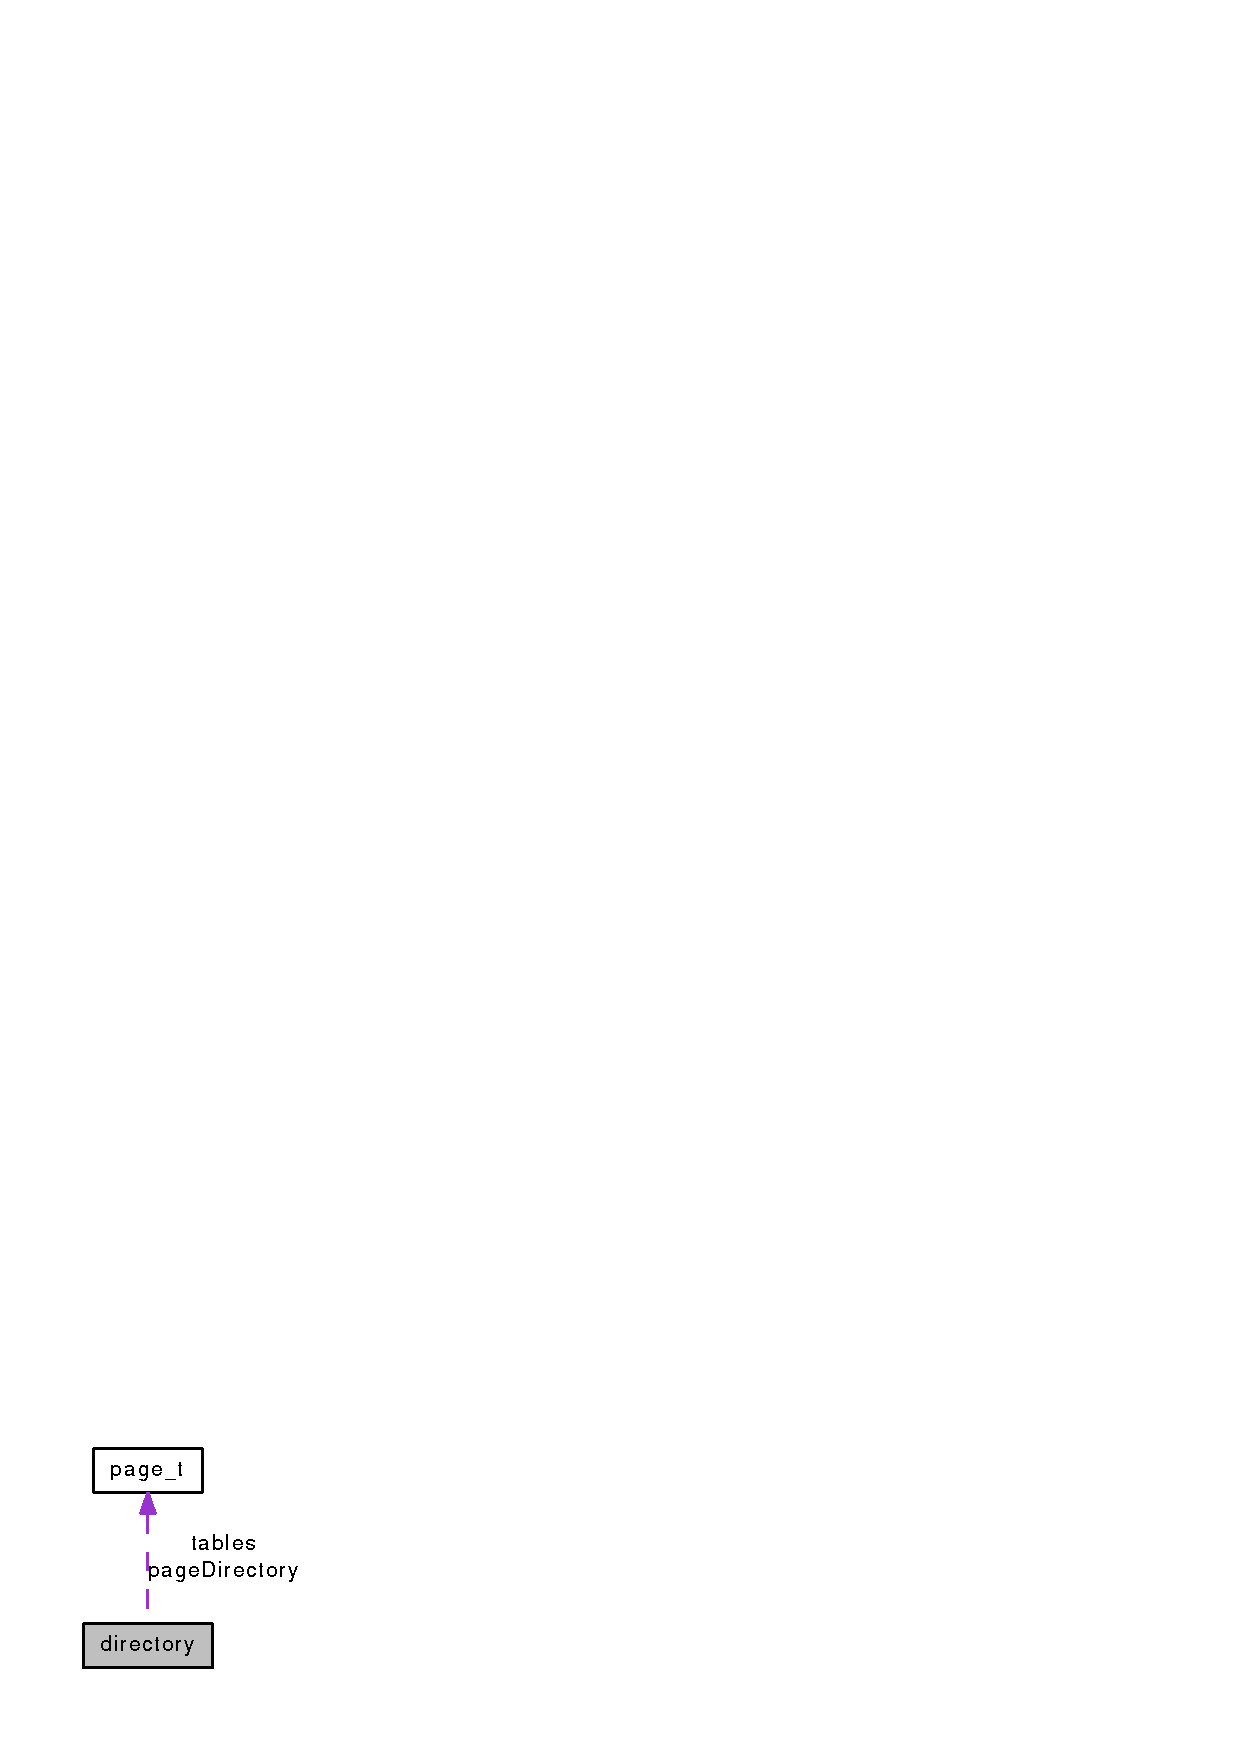
\includegraphics[width=148pt]{structdirectory__coll__graph}
\end{center}
\end{figure}
\subsection*{Data Fields}
\begin{DoxyCompactItemize}
\item 
\hyperlink{structpage_table__t}{pageTable\_\-t} \hyperlink{structdirectory_a3e0d7ce1ada814ee34fecb417f482914}{tables} \mbox{[}PAGE\_\-TABLES\_\-QTY\mbox{]}
\item 
\hyperlink{structpage_table__t}{pageTable\_\-t} \hyperlink{structdirectory_ace546e6a880b7429f91ee63ec5b6f4ca}{pageDirectory}
\end{DoxyCompactItemize}


\subsection{Detailed Description}


Definition at line 88 of file types.h.



\subsection{Field Documentation}
\hypertarget{structdirectory_ace546e6a880b7429f91ee63ec5b6f4ca}{
\index{directory@{directory}!pageDirectory@{pageDirectory}}
\index{pageDirectory@{pageDirectory}!directory@{directory}}
\subsubsection[{pageDirectory}]{\setlength{\rightskip}{0pt plus 5cm}{\bf pageTable\_\-t} {\bf pageDirectory}}}
\label{structdirectory_ace546e6a880b7429f91ee63ec5b6f4ca}


Definition at line 90 of file types.h.

\hypertarget{structdirectory_a3e0d7ce1ada814ee34fecb417f482914}{
\index{directory@{directory}!tables@{tables}}
\index{tables@{tables}!directory@{directory}}
\subsubsection[{tables}]{\setlength{\rightskip}{0pt plus 5cm}{\bf pageTable\_\-t} {\bf tables}\mbox{[}PAGE\_\-TABLES\_\-QTY\mbox{]}}}
\label{structdirectory_a3e0d7ce1ada814ee34fecb417f482914}


Definition at line 89 of file types.h.



The documentation for this struct was generated from the following file:\begin{DoxyCompactItemize}
\item 
inc/\hyperlink{types_8h}{types.h}\end{DoxyCompactItemize}

\hypertarget{structdirectory__t}{
\section{directory\_\-t Struct Reference}
\label{structdirectory__t}\index{directory\_\-t@{directory\_\-t}}
}


The page directory typedef.  




{\ttfamily \#include $<$types.h$>$}



\subsection{Detailed Description}
The page directory typedef. 

The documentation for this struct was generated from the following file:\begin{DoxyCompactItemize}
\item 
inc/\hyperlink{types_8h}{types.h}\end{DoxyCompactItemize}

\hypertarget{struct_f_i_l_e}{
\section{FILE Struct Reference}
\label{struct_f_i_l_e}\index{FILE@{FILE}}
}


The \hyperlink{struct_f_i_l_e}{FILE} struct.  




{\ttfamily \#include $<$types.h$>$}

\subsection*{Data Fields}
\begin{DoxyCompactItemize}
\item 
int \hyperlink{struct_f_i_l_e_a6f8059414f0228f0256115e024eeed4b}{fd}
\item 
char $\ast$ \hyperlink{struct_f_i_l_e_aff2566f4c366b48d73479bef43ee4d2e}{buffer}
\item 
char $\ast$ \hyperlink{struct_f_i_l_e_a935adc2e417a61d7eb6f04efb18ba031}{ptr}
\item 
int \hyperlink{struct_f_i_l_e_adf916204820072417ed73a32de1cefcf}{flag}
\item 
\hyperlink{types_8h_a7b60c5629e55e8ec87a4547dd4abced4}{size\_\-t} \hyperlink{struct_f_i_l_e_a7be887a2ca0a258cf6b368d32fd87487}{bufferSize}
\end{DoxyCompactItemize}


\subsection{Detailed Description}
The \hyperlink{struct_f_i_l_e}{FILE} struct. 

Definition at line 122 of file types.h.



\subsection{Field Documentation}
\hypertarget{struct_f_i_l_e_aff2566f4c366b48d73479bef43ee4d2e}{
\index{FILE@{FILE}!buffer@{buffer}}
\index{buffer@{buffer}!FILE@{FILE}}
\subsubsection[{buffer}]{\setlength{\rightskip}{0pt plus 5cm}char$\ast$ {\bf buffer}}}
\label{struct_f_i_l_e_aff2566f4c366b48d73479bef43ee4d2e}


Definition at line 124 of file types.h.

\hypertarget{struct_f_i_l_e_a7be887a2ca0a258cf6b368d32fd87487}{
\index{FILE@{FILE}!bufferSize@{bufferSize}}
\index{bufferSize@{bufferSize}!FILE@{FILE}}
\subsubsection[{bufferSize}]{\setlength{\rightskip}{0pt plus 5cm}{\bf size\_\-t} {\bf bufferSize}}}
\label{struct_f_i_l_e_a7be887a2ca0a258cf6b368d32fd87487}


Definition at line 127 of file types.h.

\hypertarget{struct_f_i_l_e_a6f8059414f0228f0256115e024eeed4b}{
\index{FILE@{FILE}!fd@{fd}}
\index{fd@{fd}!FILE@{FILE}}
\subsubsection[{fd}]{\setlength{\rightskip}{0pt plus 5cm}int {\bf fd}}}
\label{struct_f_i_l_e_a6f8059414f0228f0256115e024eeed4b}


Definition at line 123 of file types.h.

\hypertarget{struct_f_i_l_e_adf916204820072417ed73a32de1cefcf}{
\index{FILE@{FILE}!flag@{flag}}
\index{flag@{flag}!FILE@{FILE}}
\subsubsection[{flag}]{\setlength{\rightskip}{0pt plus 5cm}int {\bf flag}}}
\label{struct_f_i_l_e_adf916204820072417ed73a32de1cefcf}


Definition at line 126 of file types.h.

\hypertarget{struct_f_i_l_e_a935adc2e417a61d7eb6f04efb18ba031}{
\index{FILE@{FILE}!ptr@{ptr}}
\index{ptr@{ptr}!FILE@{FILE}}
\subsubsection[{ptr}]{\setlength{\rightskip}{0pt plus 5cm}char$\ast$ {\bf ptr}}}
\label{struct_f_i_l_e_a935adc2e417a61d7eb6f04efb18ba031}


Definition at line 125 of file types.h.



The documentation for this struct was generated from the following file:\begin{DoxyCompactItemize}
\item 
inc/\hyperlink{types_8h}{types.h}\end{DoxyCompactItemize}

\hypertarget{structframe}{
\section{frame Struct Reference}
\label{structframe}\index{frame@{frame}}
}


{\ttfamily \#include $<$types.h$>$}

\subsection*{Data Fields}
\begin{DoxyCompactItemize}
\item 
int \hyperlink{structframe_a2602074f4e3c3e245e59f512aa565fcc}{assigned}
\item 
unsigned int \hyperlink{structframe_a2f55ff1f6cd45ca1b6431493ab5614eb}{address}
\end{DoxyCompactItemize}


\subsection{Detailed Description}


Definition at line 97 of file types.h.



\subsection{Field Documentation}
\hypertarget{structframe_a2f55ff1f6cd45ca1b6431493ab5614eb}{
\index{frame@{frame}!address@{address}}
\index{address@{address}!frame@{frame}}
\subsubsection[{address}]{\setlength{\rightskip}{0pt plus 5cm}unsigned int {\bf address}}}
\label{structframe_a2f55ff1f6cd45ca1b6431493ab5614eb}


Definition at line 99 of file types.h.

\hypertarget{structframe_a2602074f4e3c3e245e59f512aa565fcc}{
\index{frame@{frame}!assigned@{assigned}}
\index{assigned@{assigned}!frame@{frame}}
\subsubsection[{assigned}]{\setlength{\rightskip}{0pt plus 5cm}int {\bf assigned}}}
\label{structframe_a2602074f4e3c3e245e59f512aa565fcc}


Definition at line 98 of file types.h.



The documentation for this struct was generated from the following file:\begin{DoxyCompactItemize}
\item 
inc/\hyperlink{types_8h}{types.h}\end{DoxyCompactItemize}

\hypertarget{structframe__t}{
\section{frame\_\-t Struct Reference}
\label{structframe__t}\index{frame\_\-t@{frame\_\-t}}
}


The page frame struct.  




{\ttfamily \#include $<$types.h$>$}



\subsection{Detailed Description}
The page frame struct. 

The documentation for this struct was generated from the following file:\begin{DoxyCompactItemize}
\item 
inc/\hyperlink{types_8h}{types.h}\end{DoxyCompactItemize}

\hypertarget{structframes_table__t}{
\section{framesTable\_\-t Struct Reference}
\label{structframes_table__t}\index{framesTable\_\-t@{framesTable\_\-t}}
}


The frames table typedef.  




{\ttfamily \#include $<$types.h$>$}



\subsection{Detailed Description}
The frames table typedef. 

The documentation for this struct was generated from the following file:\begin{DoxyCompactItemize}
\item 
inc/\hyperlink{types_8h}{types.h}\end{DoxyCompactItemize}

\hypertarget{structheap_status}{
\section{heapStatus Struct Reference}
\label{structheap_status}\index{heapStatus@{heapStatus}}
}


The heap status struct.  




{\ttfamily \#include $<$types.h$>$}



Collaboration diagram for heapStatus:\nopagebreak
\begin{figure}[H]
\begin{center}
\leavevmode
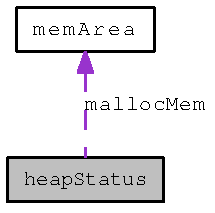
\includegraphics[width=139pt]{structheap_status__coll__graph}
\end{center}
\end{figure}
\subsection*{Data Fields}
\begin{DoxyCompactItemize}
\item 
int \hyperlink{structheap_status_aa6ddfc2b6fa7dd2f05f6226e7d41d3a2}{asigment}
\item 
\hyperlink{structmem_area__t}{memArea\_\-t} \hyperlink{structheap_status_a563eaaea14f23514bd4a6c87f11711dd}{mallocMem}
\end{DoxyCompactItemize}


\subsection{Detailed Description}
The heap status struct. 

Definition at line 134 of file types.h.



\subsection{Field Documentation}
\hypertarget{structheap_status_aa6ddfc2b6fa7dd2f05f6226e7d41d3a2}{
\index{heapStatus@{heapStatus}!asigment@{asigment}}
\index{asigment@{asigment}!heapStatus@{heapStatus}}
\subsubsection[{asigment}]{\setlength{\rightskip}{0pt plus 5cm}int {\bf asigment}}}
\label{structheap_status_aa6ddfc2b6fa7dd2f05f6226e7d41d3a2}


Definition at line 135 of file types.h.

\hypertarget{structheap_status_a563eaaea14f23514bd4a6c87f11711dd}{
\index{heapStatus@{heapStatus}!mallocMem@{mallocMem}}
\index{mallocMem@{mallocMem}!heapStatus@{heapStatus}}
\subsubsection[{mallocMem}]{\setlength{\rightskip}{0pt plus 5cm}{\bf memArea\_\-t} {\bf mallocMem}}}
\label{structheap_status_a563eaaea14f23514bd4a6c87f11711dd}


Definition at line 136 of file types.h.



The documentation for this struct was generated from the following file:\begin{DoxyCompactItemize}
\item 
inc/\hyperlink{types_8h}{types.h}\end{DoxyCompactItemize}

\hypertarget{struct_i_d_t_r}{
\section{IDTR Struct Reference}
\label{struct_i_d_t_r}\index{IDTR@{IDTR}}
}


OS \hyperlink{struct_i_d_t_r}{IDTR} struct.  




{\ttfamily \#include $<$types.h$>$}

\subsection*{Data Fields}
\begin{DoxyCompactItemize}
\item 
word \hyperlink{struct_i_d_t_r_ab5c3c0a36eb16002f03ae8565e505e89}{limit}
\item 
dword \hyperlink{struct_i_d_t_r_acdee40c1e899300b428fdaee620723e5}{base}
\end{DoxyCompactItemize}


\subsection{Detailed Description}
OS \hyperlink{struct_i_d_t_r}{IDTR} struct. 

Definition at line 363 of file types.h.



\subsection{Field Documentation}
\hypertarget{struct_i_d_t_r_acdee40c1e899300b428fdaee620723e5}{
\index{IDTR@{IDTR}!base@{base}}
\index{base@{base}!IDTR@{IDTR}}
\subsubsection[{base}]{\setlength{\rightskip}{0pt plus 5cm}dword {\bf base}}}
\label{struct_i_d_t_r_acdee40c1e899300b428fdaee620723e5}


Definition at line 365 of file types.h.

\hypertarget{struct_i_d_t_r_ab5c3c0a36eb16002f03ae8565e505e89}{
\index{IDTR@{IDTR}!limit@{limit}}
\index{limit@{limit}!IDTR@{IDTR}}
\subsubsection[{limit}]{\setlength{\rightskip}{0pt plus 5cm}word {\bf limit}}}
\label{struct_i_d_t_r_ab5c3c0a36eb16002f03ae8565e505e89}


Definition at line 364 of file types.h.



The documentation for this struct was generated from the following file:\begin{DoxyCompactItemize}
\item 
inc/\hyperlink{types_8h}{types.h}\end{DoxyCompactItemize}

\hypertarget{structindexed_buffer}{
\section{indexedBuffer Struct Reference}
\label{structindexed_buffer}\index{indexedBuffer@{indexedBuffer}}
}
\subsection*{Data Fields}
\begin{DoxyCompactItemize}
\item 
void $\ast$ \hyperlink{structindexed_buffer_a368f7094dc38acca20612bbb392552f4}{buffer}
\item 
int \hyperlink{structindexed_buffer_a750b5d744c39a06bfb13e6eb010e35d0}{index}
\end{DoxyCompactItemize}


\subsection{Detailed Description}


Definition at line 143 of file video\_\-driver.c.



\subsection{Field Documentation}
\hypertarget{structindexed_buffer_a368f7094dc38acca20612bbb392552f4}{
\index{indexedBuffer@{indexedBuffer}!buffer@{buffer}}
\index{buffer@{buffer}!indexedBuffer@{indexedBuffer}}
\subsubsection[{buffer}]{\setlength{\rightskip}{0pt plus 5cm}void$\ast$ {\bf buffer}}}
\label{structindexed_buffer_a368f7094dc38acca20612bbb392552f4}


Definition at line 144 of file video\_\-driver.c.

\hypertarget{structindexed_buffer_a750b5d744c39a06bfb13e6eb010e35d0}{
\index{indexedBuffer@{indexedBuffer}!index@{index}}
\index{index@{index}!indexedBuffer@{indexedBuffer}}
\subsubsection[{index}]{\setlength{\rightskip}{0pt plus 5cm}int {\bf index}}}
\label{structindexed_buffer_a750b5d744c39a06bfb13e6eb010e35d0}


Definition at line 145 of file video\_\-driver.c.



The documentation for this struct was generated from the following file:\begin{DoxyCompactItemize}
\item 
src/\hyperlink{video__driver_8c}{video\_\-driver.c}\end{DoxyCompactItemize}

\hypertarget{structlist_with_prio}{
\section{listWithPrio Struct Reference}
\label{structlist_with_prio}\index{listWithPrio@{listWithPrio}}
}


Collaboration diagram for listWithPrio:\nopagebreak
\begin{figure}[H]
\begin{center}
\leavevmode
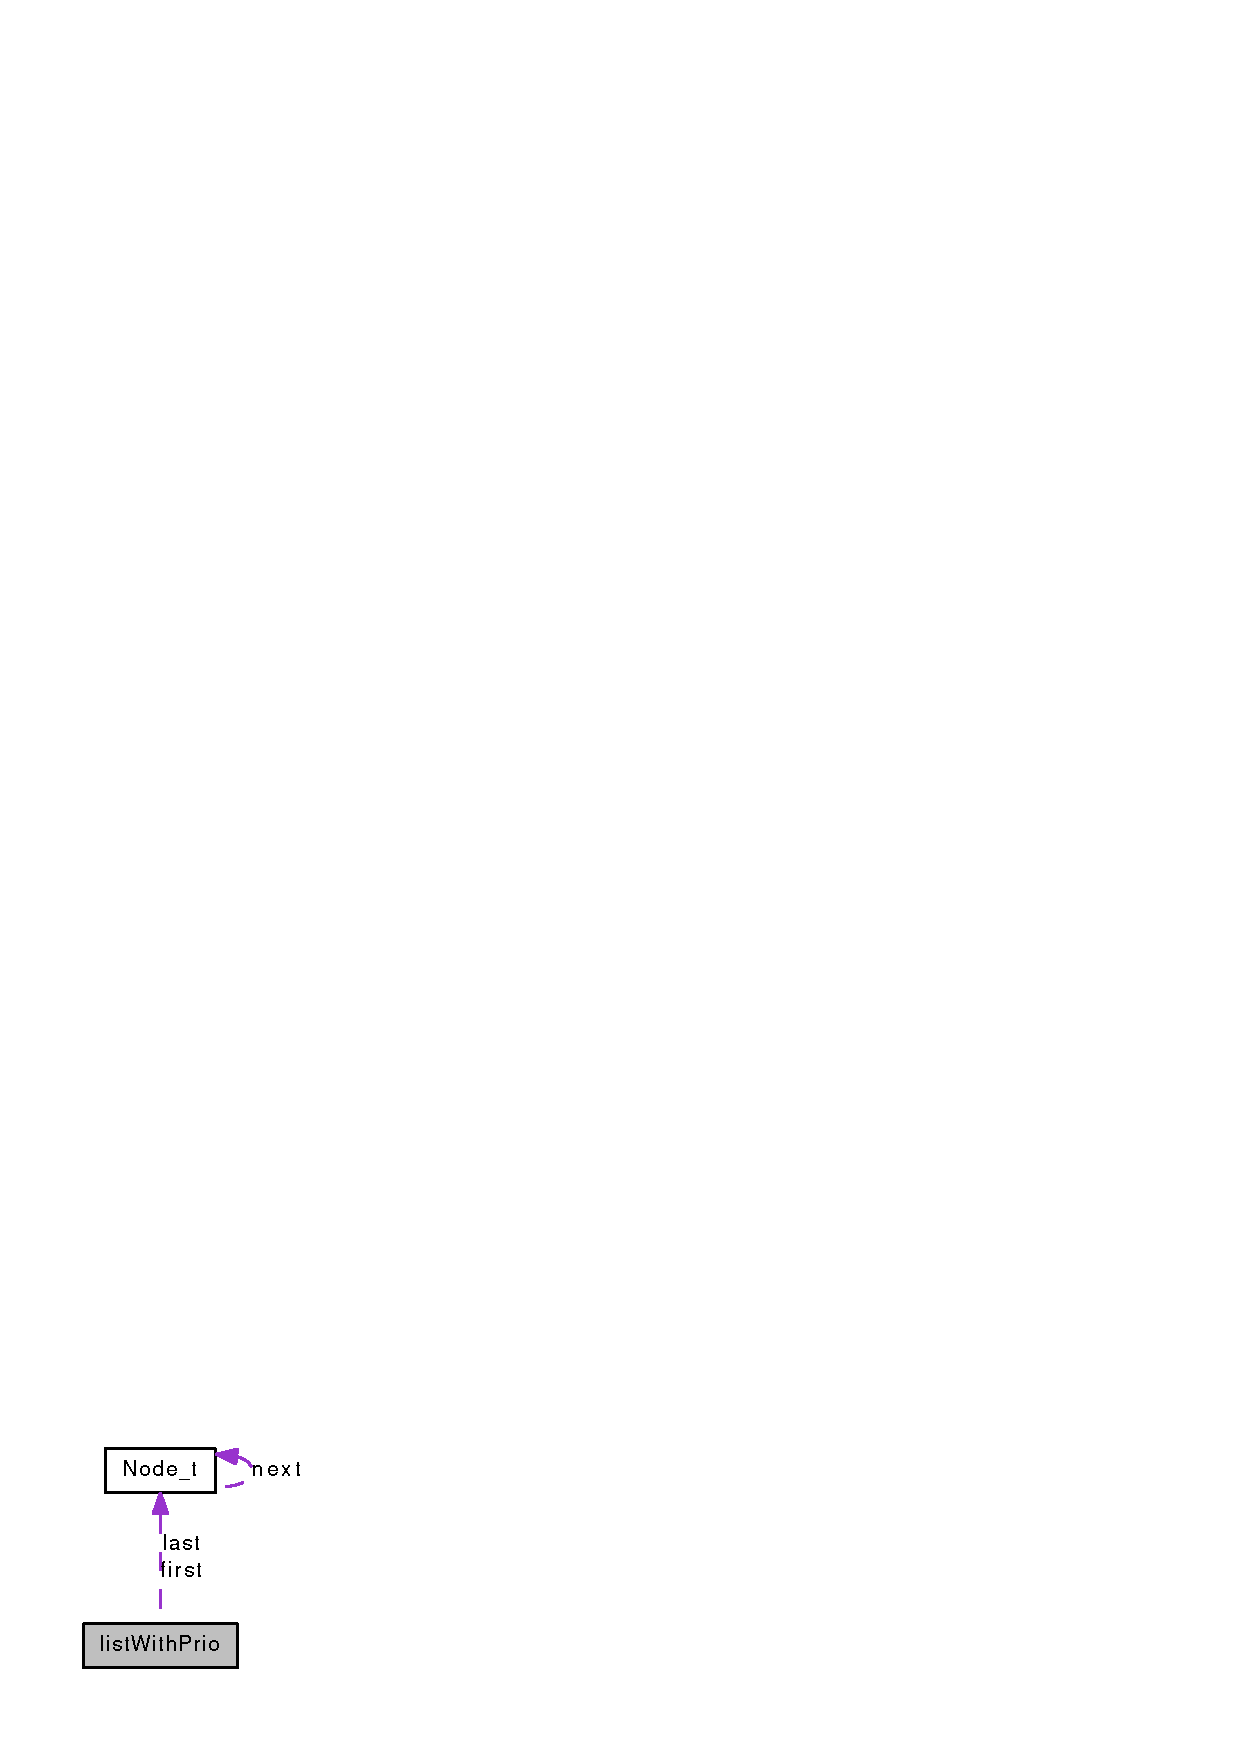
\includegraphics[width=150pt]{structlist_with_prio__coll__graph}
\end{center}
\end{figure}
\subsection*{Data Fields}
\begin{DoxyCompactItemize}
\item 
int \hyperlink{structlist_with_prio_acec9ce2df15222151ad66fcb1d74eb9f}{priority}
\item 
int \hyperlink{structlist_with_prio_a671979afa869339d57da6ad30c0498d8}{pQueueDim}
\item 
\hyperlink{struct_node__t}{Node\_\-t} $\ast$ \hyperlink{structlist_with_prio_aaea2707399dfe92afae4ef90749f7542}{first}
\item 
\hyperlink{struct_node__t}{Node\_\-t} $\ast$ \hyperlink{structlist_with_prio_a1b88fdeb724166cbdf6717d7ba4b49c6}{last}
\end{DoxyCompactItemize}


\subsection{Detailed Description}


Definition at line 24 of file pQueueP.c.



\subsection{Field Documentation}
\hypertarget{structlist_with_prio_aaea2707399dfe92afae4ef90749f7542}{
\index{listWithPrio@{listWithPrio}!first@{first}}
\index{first@{first}!listWithPrio@{listWithPrio}}
\subsubsection[{first}]{\setlength{\rightskip}{0pt plus 5cm}{\bf Node\_\-t}$\ast$ {\bf first}}}
\label{structlist_with_prio_aaea2707399dfe92afae4ef90749f7542}


Definition at line 27 of file pQueueP.c.

\hypertarget{structlist_with_prio_a1b88fdeb724166cbdf6717d7ba4b49c6}{
\index{listWithPrio@{listWithPrio}!last@{last}}
\index{last@{last}!listWithPrio@{listWithPrio}}
\subsubsection[{last}]{\setlength{\rightskip}{0pt plus 5cm}{\bf Node\_\-t}$\ast$ {\bf last}}}
\label{structlist_with_prio_a1b88fdeb724166cbdf6717d7ba4b49c6}


Definition at line 28 of file pQueueP.c.

\hypertarget{structlist_with_prio_a671979afa869339d57da6ad30c0498d8}{
\index{listWithPrio@{listWithPrio}!pQueueDim@{pQueueDim}}
\index{pQueueDim@{pQueueDim}!listWithPrio@{listWithPrio}}
\subsubsection[{pQueueDim}]{\setlength{\rightskip}{0pt plus 5cm}int {\bf pQueueDim}}}
\label{structlist_with_prio_a671979afa869339d57da6ad30c0498d8}


Definition at line 26 of file pQueueP.c.

\hypertarget{structlist_with_prio_acec9ce2df15222151ad66fcb1d74eb9f}{
\index{listWithPrio@{listWithPrio}!priority@{priority}}
\index{priority@{priority}!listWithPrio@{listWithPrio}}
\subsubsection[{priority}]{\setlength{\rightskip}{0pt plus 5cm}int {\bf priority}}}
\label{structlist_with_prio_acec9ce2df15222151ad66fcb1d74eb9f}


Definition at line 25 of file pQueueP.c.



The documentation for this struct was generated from the following file:\begin{DoxyCompactItemize}
\item 
src/\hyperlink{p_queue_p_8c}{pQueueP.c}\end{DoxyCompactItemize}

\hypertarget{structmem_area}{
\section{memArea Struct Reference}
\label{structmem_area}\index{memArea@{memArea}}
}


{\ttfamily \#include $<$types.h$>$}

\subsection*{Data Fields}
\begin{DoxyCompactItemize}
\item 
void $\ast$ \hyperlink{structmem_area_ab96816d317aa5196e2ef198d9a8d621b}{address}
\item 
\hyperlink{types_8h_a7b60c5629e55e8ec87a4547dd4abced4}{size\_\-t} \hyperlink{structmem_area_a854352f53b148adc24983a58a1866d66}{size}
\item 
char $\ast$ \hyperlink{structmem_area_aa781caae63dbdaa07fcac17a08e4f048}{allocp}
\end{DoxyCompactItemize}


\subsection{Detailed Description}


Definition at line 106 of file types.h.



\subsection{Field Documentation}
\hypertarget{structmem_area_ab96816d317aa5196e2ef198d9a8d621b}{
\index{memArea@{memArea}!address@{address}}
\index{address@{address}!memArea@{memArea}}
\subsubsection[{address}]{\setlength{\rightskip}{0pt plus 5cm}void$\ast$ {\bf address}}}
\label{structmem_area_ab96816d317aa5196e2ef198d9a8d621b}


Definition at line 107 of file types.h.

\hypertarget{structmem_area_aa781caae63dbdaa07fcac17a08e4f048}{
\index{memArea@{memArea}!allocp@{allocp}}
\index{allocp@{allocp}!memArea@{memArea}}
\subsubsection[{allocp}]{\setlength{\rightskip}{0pt plus 5cm}char$\ast$ {\bf allocp}}}
\label{structmem_area_aa781caae63dbdaa07fcac17a08e4f048}


Definition at line 109 of file types.h.

\hypertarget{structmem_area_a854352f53b148adc24983a58a1866d66}{
\index{memArea@{memArea}!size@{size}}
\index{size@{size}!memArea@{memArea}}
\subsubsection[{size}]{\setlength{\rightskip}{0pt plus 5cm}{\bf size\_\-t} {\bf size}}}
\label{structmem_area_a854352f53b148adc24983a58a1866d66}


Definition at line 108 of file types.h.



The documentation for this struct was generated from the following file:\begin{DoxyCompactItemize}
\item 
inc/\hyperlink{types_8h}{types.h}\end{DoxyCompactItemize}

\hypertarget{structmem_area__t}{
\section{memArea\_\-t Struct Reference}
\label{structmem_area__t}\index{memArea\_\-t@{memArea\_\-t}}
}


The mem area malloc struct.  




{\ttfamily \#include $<$types.h$>$}



\subsection{Detailed Description}
The mem area malloc struct. 

The documentation for this struct was generated from the following file:\begin{DoxyCompactItemize}
\item 
inc/\hyperlink{types_8h}{types.h}\end{DoxyCompactItemize}

\hypertarget{struct_node__t}{
\section{Node\_\-t Struct Reference}
\label{struct_node__t}\index{Node\_\-t@{Node\_\-t}}
}


Collaboration diagram for Node\_\-t:\nopagebreak
\begin{figure}[H]
\begin{center}
\leavevmode
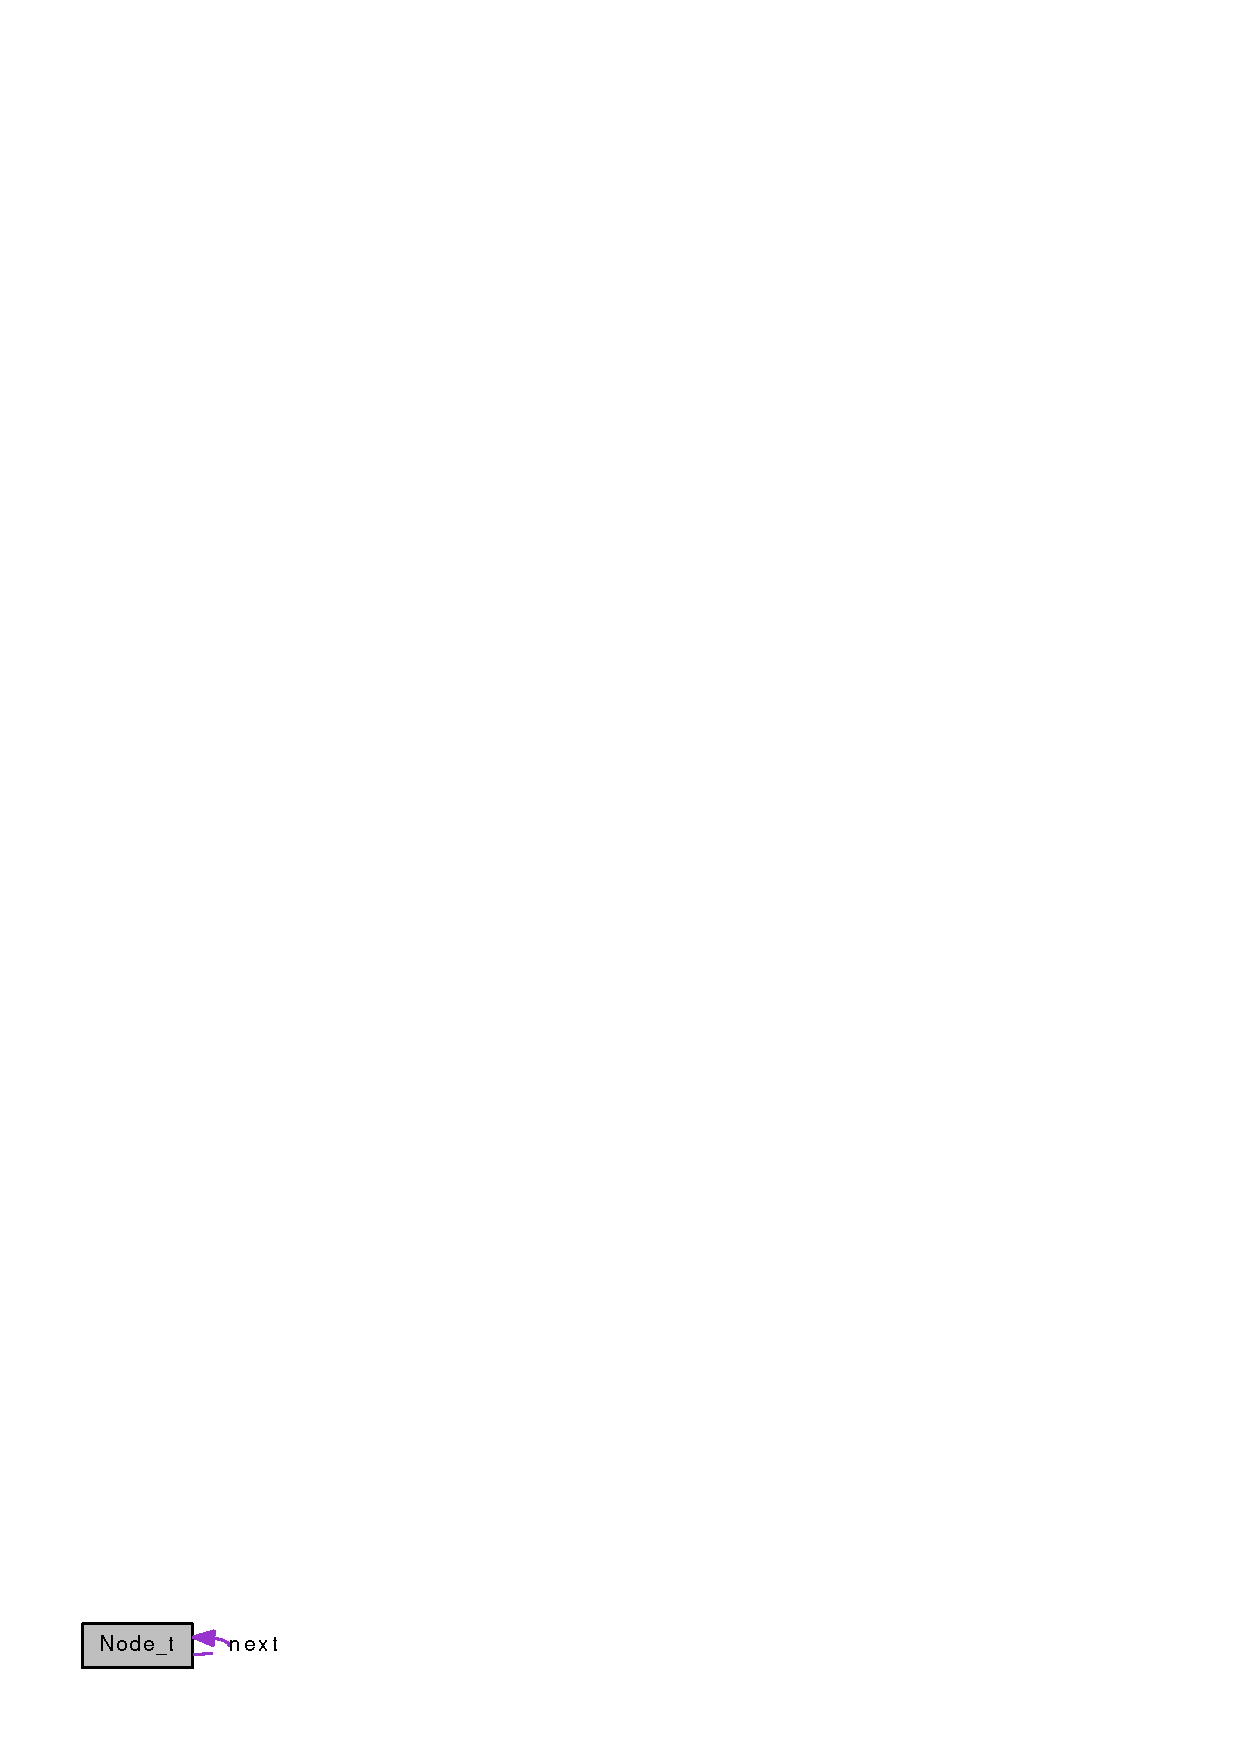
\includegraphics[width=139pt]{struct_node__t__coll__graph}
\end{center}
\end{figure}
\subsection*{Data Fields}
\begin{DoxyCompactItemize}
\item 
void $\ast$ \hyperlink{struct_node__t_a735984d41155bc1032e09bece8f8d66d}{data}
\item 
struct \hyperlink{struct_node__t}{Node\_\-t} $\ast$ \hyperlink{struct_node__t_a5e58c48351200ad246d4db491634433c}{next}
\end{DoxyCompactItemize}


\subsection{Detailed Description}


Definition at line 19 of file pQueueP.c.



\subsection{Field Documentation}
\hypertarget{struct_node__t_a735984d41155bc1032e09bece8f8d66d}{
\index{Node\_\-t@{Node\_\-t}!data@{data}}
\index{data@{data}!Node_t@{Node\_\-t}}
\subsubsection[{data}]{\setlength{\rightskip}{0pt plus 5cm}void$\ast$ {\bf data}}}
\label{struct_node__t_a735984d41155bc1032e09bece8f8d66d}


Definition at line 15 of file pQueueP.c.

\hypertarget{struct_node__t_a5e58c48351200ad246d4db491634433c}{
\index{Node\_\-t@{Node\_\-t}!next@{next}}
\index{next@{next}!Node_t@{Node\_\-t}}
\subsubsection[{next}]{\setlength{\rightskip}{0pt plus 5cm}struct {\bf Node\_\-t}$\ast$ {\bf next}}}
\label{struct_node__t_a5e58c48351200ad246d4db491634433c}


Definition at line 16 of file pQueueP.c.



The documentation for this struct was generated from the following file:\begin{DoxyCompactItemize}
\item 
src/\hyperlink{p_queue_p_8c}{pQueueP.c}\end{DoxyCompactItemize}

\hypertarget{structpage}{
\section{page Struct Reference}
\label{structpage}\index{page@{page}}
}


{\ttfamily \#include $<$types.h$>$}

\subsection*{Data Fields}
\begin{DoxyCompactItemize}
\item 
unsigned int \hyperlink{structpage_abc4c133346e4b24e2e71fe80ffc39a6f}{present}: 1
\item 
unsigned int \hyperlink{structpage_a053ea5deda2f64604e4541bf626bef9c}{writeable}: 1
\item 
unsigned int \hyperlink{structpage_aaf4a05f547280bd4819e5df8c4523cd1}{user}: 1
\item 
unsigned int \hyperlink{structpage_a8bcb7dbeb8dba19debc9a4a062f8a6bc}{directWrite}: 1
\item 
unsigned int \hyperlink{structpage_afed734c6ffccf36d8318903bfe4e4e1b}{disableCache}: 1
\item 
unsigned int \hyperlink{structpage_ad9199508706a6aaec358e5200bb389c7}{accessed}: 1
\item 
unsigned int \hyperlink{structpage_a930a1ab0130f619f847727300b9d156a}{dirty}: 1
\item 
unsigned int \hyperlink{structpage_a05d5cbcb44f437341bd9fa37d589aced}{reserved}: 5
\item 
unsigned int \hyperlink{structpage_a2f55ff1f6cd45ca1b6431493ab5614eb}{address}: 20
\end{DoxyCompactItemize}


\subsection{Detailed Description}


Definition at line 66 of file types.h.



\subsection{Field Documentation}
\hypertarget{structpage_ad9199508706a6aaec358e5200bb389c7}{
\index{page@{page}!accessed@{accessed}}
\index{accessed@{accessed}!page@{page}}
\subsubsection[{accessed}]{\setlength{\rightskip}{0pt plus 5cm}unsigned int {\bf accessed}}}
\label{structpage_ad9199508706a6aaec358e5200bb389c7}


Definition at line 72 of file types.h.

\hypertarget{structpage_a2f55ff1f6cd45ca1b6431493ab5614eb}{
\index{page@{page}!address@{address}}
\index{address@{address}!page@{page}}
\subsubsection[{address}]{\setlength{\rightskip}{0pt plus 5cm}unsigned int {\bf address}}}
\label{structpage_a2f55ff1f6cd45ca1b6431493ab5614eb}


Definition at line 75 of file types.h.

\hypertarget{structpage_a8bcb7dbeb8dba19debc9a4a062f8a6bc}{
\index{page@{page}!directWrite@{directWrite}}
\index{directWrite@{directWrite}!page@{page}}
\subsubsection[{directWrite}]{\setlength{\rightskip}{0pt plus 5cm}unsigned int {\bf directWrite}}}
\label{structpage_a8bcb7dbeb8dba19debc9a4a062f8a6bc}


Definition at line 70 of file types.h.

\hypertarget{structpage_a930a1ab0130f619f847727300b9d156a}{
\index{page@{page}!dirty@{dirty}}
\index{dirty@{dirty}!page@{page}}
\subsubsection[{dirty}]{\setlength{\rightskip}{0pt plus 5cm}unsigned int {\bf dirty}}}
\label{structpage_a930a1ab0130f619f847727300b9d156a}


Definition at line 73 of file types.h.

\hypertarget{structpage_afed734c6ffccf36d8318903bfe4e4e1b}{
\index{page@{page}!disableCache@{disableCache}}
\index{disableCache@{disableCache}!page@{page}}
\subsubsection[{disableCache}]{\setlength{\rightskip}{0pt plus 5cm}unsigned int {\bf disableCache}}}
\label{structpage_afed734c6ffccf36d8318903bfe4e4e1b}


Definition at line 71 of file types.h.

\hypertarget{structpage_abc4c133346e4b24e2e71fe80ffc39a6f}{
\index{page@{page}!present@{present}}
\index{present@{present}!page@{page}}
\subsubsection[{present}]{\setlength{\rightskip}{0pt plus 5cm}unsigned int {\bf present}}}
\label{structpage_abc4c133346e4b24e2e71fe80ffc39a6f}


Definition at line 67 of file types.h.

\hypertarget{structpage_a05d5cbcb44f437341bd9fa37d589aced}{
\index{page@{page}!reserved@{reserved}}
\index{reserved@{reserved}!page@{page}}
\subsubsection[{reserved}]{\setlength{\rightskip}{0pt plus 5cm}unsigned int {\bf reserved}}}
\label{structpage_a05d5cbcb44f437341bd9fa37d589aced}


Definition at line 74 of file types.h.

\hypertarget{structpage_aaf4a05f547280bd4819e5df8c4523cd1}{
\index{page@{page}!user@{user}}
\index{user@{user}!page@{page}}
\subsubsection[{user}]{\setlength{\rightskip}{0pt plus 5cm}unsigned int {\bf user}}}
\label{structpage_aaf4a05f547280bd4819e5df8c4523cd1}


Definition at line 69 of file types.h.

\hypertarget{structpage_a053ea5deda2f64604e4541bf626bef9c}{
\index{page@{page}!writeable@{writeable}}
\index{writeable@{writeable}!page@{page}}
\subsubsection[{writeable}]{\setlength{\rightskip}{0pt plus 5cm}unsigned int {\bf writeable}}}
\label{structpage_a053ea5deda2f64604e4541bf626bef9c}


Definition at line 68 of file types.h.



The documentation for this struct was generated from the following file:\begin{DoxyCompactItemize}
\item 
inc/\hyperlink{types_8h}{types.h}\end{DoxyCompactItemize}

\hypertarget{structpage__t}{
\section{page\_\-t Struct Reference}
\label{structpage__t}\index{page\_\-t@{page\_\-t}}
}


The paging page struct.  




{\ttfamily \#include $<$types.h$>$}



\subsection{Detailed Description}
The paging page struct. 

The documentation for this struct was generated from the following file:\begin{DoxyCompactItemize}
\item 
inc/\hyperlink{types_8h}{types.h}\end{DoxyCompactItemize}

\hypertarget{structpage_table__t}{
\section{pageTable\_\-t Struct Reference}
\label{structpage_table__t}\index{pageTable\_\-t@{pageTable\_\-t}}
}


The page table typedef.  




{\ttfamily \#include $<$types.h$>$}



\subsection{Detailed Description}
The page table typedef. 

The documentation for this struct was generated from the following file:\begin{DoxyCompactItemize}
\item 
inc/\hyperlink{types_8h}{types.h}\end{DoxyCompactItemize}

\hypertarget{structp_queue_c_d_t}{
\section{pQueueCDT Struct Reference}
\label{structp_queue_c_d_t}\index{pQueueCDT@{pQueueCDT}}
}


Collaboration diagram for pQueueCDT:\nopagebreak
\begin{figure}[H]
\begin{center}
\leavevmode
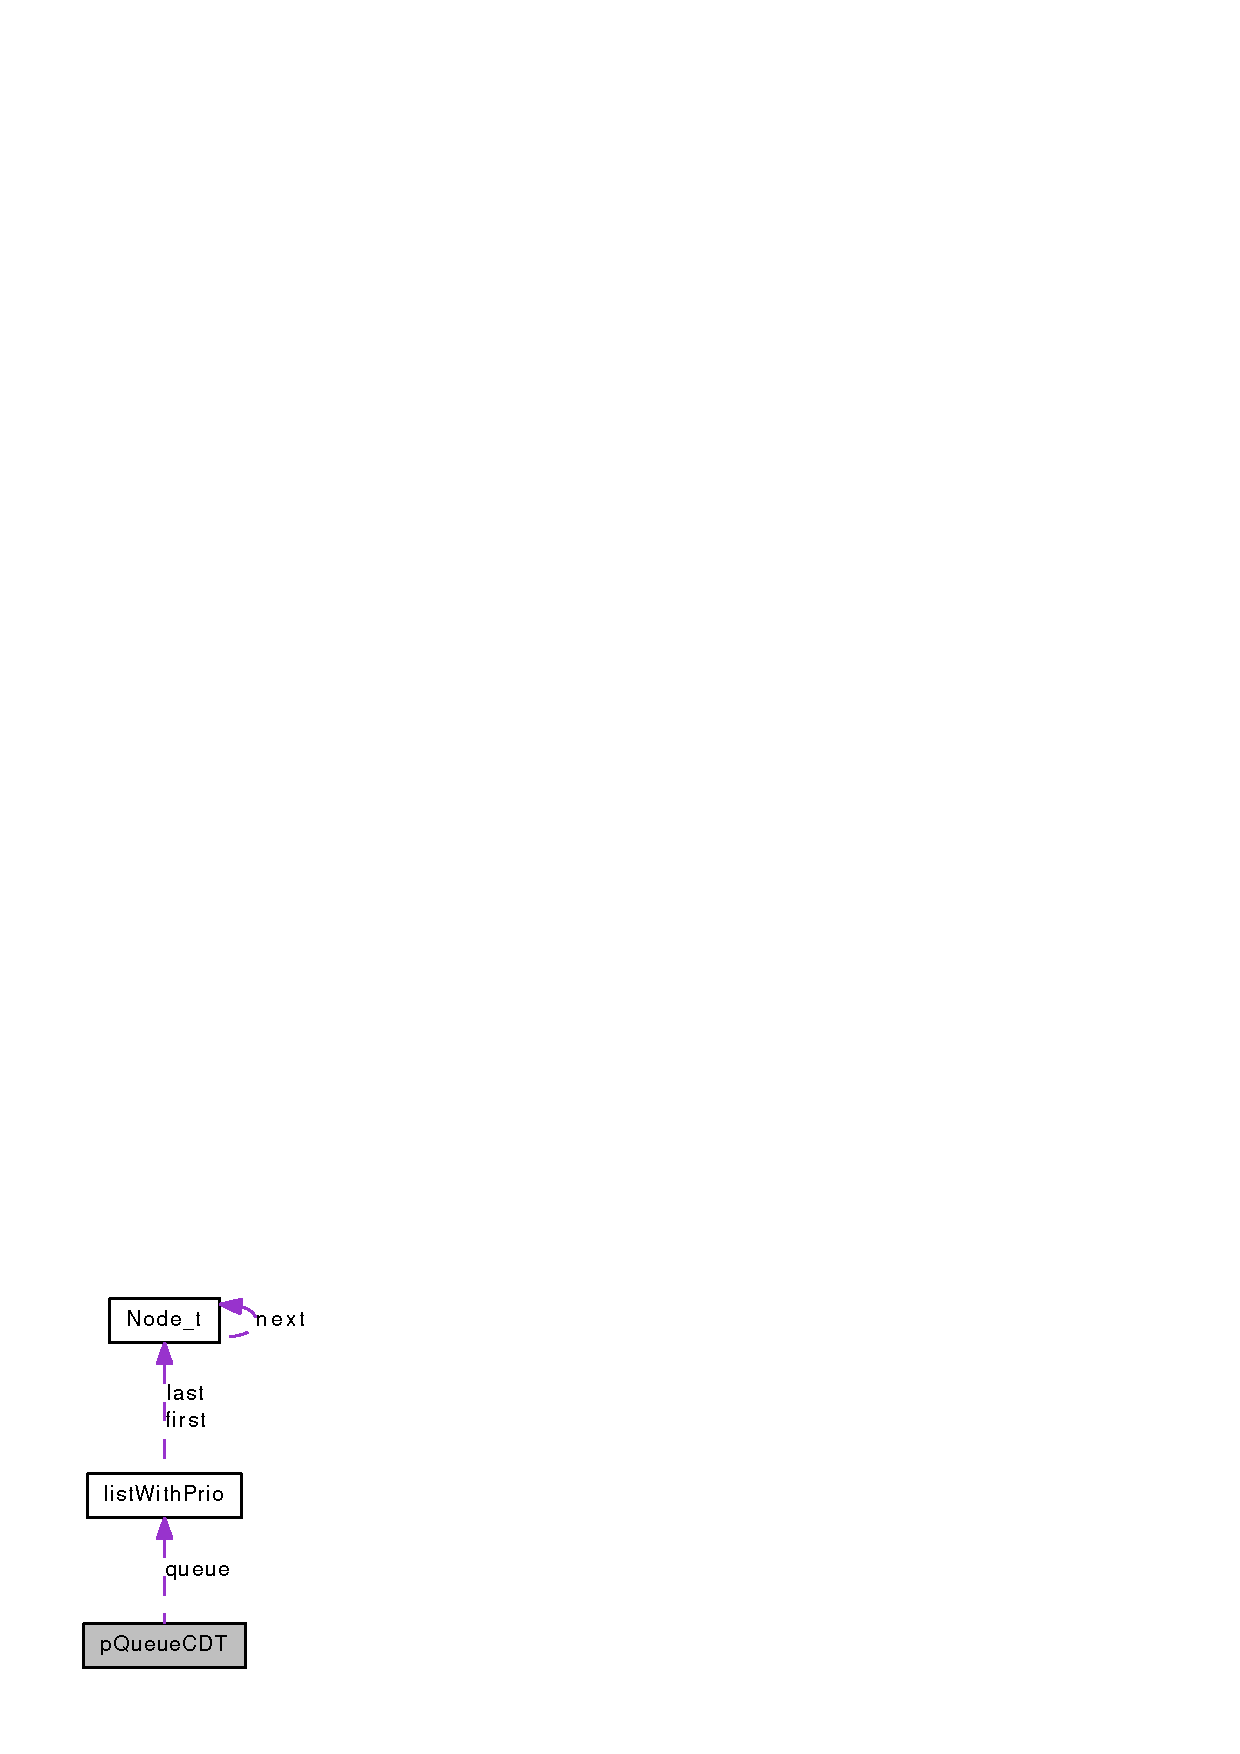
\includegraphics[width=152pt]{structp_queue_c_d_t__coll__graph}
\end{center}
\end{figure}
\subsection*{Data Fields}
\begin{DoxyCompactItemize}
\item 
\hyperlink{structlist_with_prio}{listWithPrio} $\ast$ \hyperlink{structp_queue_c_d_t_abd678f8ea5d396a97fd1938b4df23841}{queue}
\item 
void $\ast$($\ast$ \hyperlink{structp_queue_c_d_t_abce72dff83b4c0563783ac39950547ac}{cpyFn} )(void $\ast$)
\item 
void($\ast$ \hyperlink{structp_queue_c_d_t_a1ea7dba004336f82292919dfead1aceb}{freeFn} )(void $\ast$)
\end{DoxyCompactItemize}


\subsection{Detailed Description}


Definition at line 31 of file pQueueP.c.



\subsection{Field Documentation}
\hypertarget{structp_queue_c_d_t_abce72dff83b4c0563783ac39950547ac}{
\index{pQueueCDT@{pQueueCDT}!cpyFn@{cpyFn}}
\index{cpyFn@{cpyFn}!pQueueCDT@{pQueueCDT}}
\subsubsection[{cpyFn}]{\setlength{\rightskip}{0pt plus 5cm}void$\ast$($\ast$ {\bf cpyFn})(void $\ast$)}}
\label{structp_queue_c_d_t_abce72dff83b4c0563783ac39950547ac}


Definition at line 33 of file pQueueP.c.

\hypertarget{structp_queue_c_d_t_a1ea7dba004336f82292919dfead1aceb}{
\index{pQueueCDT@{pQueueCDT}!freeFn@{freeFn}}
\index{freeFn@{freeFn}!pQueueCDT@{pQueueCDT}}
\subsubsection[{freeFn}]{\setlength{\rightskip}{0pt plus 5cm}void($\ast$ {\bf freeFn})(void $\ast$)}}
\label{structp_queue_c_d_t_a1ea7dba004336f82292919dfead1aceb}


Definition at line 34 of file pQueueP.c.

\hypertarget{structp_queue_c_d_t_abd678f8ea5d396a97fd1938b4df23841}{
\index{pQueueCDT@{pQueueCDT}!queue@{queue}}
\index{queue@{queue}!pQueueCDT@{pQueueCDT}}
\subsubsection[{queue}]{\setlength{\rightskip}{0pt plus 5cm}{\bf listWithPrio}$\ast$ {\bf queue}}}
\label{structp_queue_c_d_t_abd678f8ea5d396a97fd1938b4df23841}


Definition at line 32 of file pQueueP.c.



The documentation for this struct was generated from the following file:\begin{DoxyCompactItemize}
\item 
src/\hyperlink{p_queue_p_8c}{pQueueP.c}\end{DoxyCompactItemize}

\hypertarget{structprocess__t}{
\section{process\_\-t Struct Reference}
\label{structprocess__t}\index{process\_\-t@{process\_\-t}}
}


The process struct.  




{\ttfamily \#include $<$types.h$>$}



Collaboration diagram for process\_\-t:\nopagebreak
\begin{figure}[H]
\begin{center}
\leavevmode
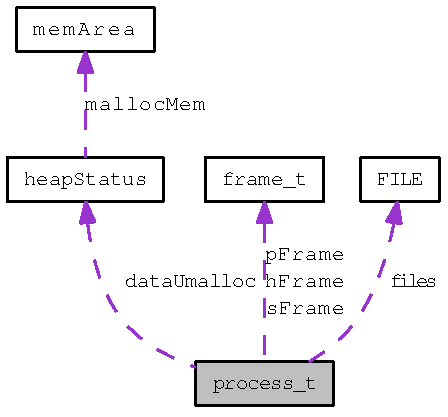
\includegraphics[width=251pt]{structprocess__t__coll__graph}
\end{center}
\end{figure}
\subsection*{Data Fields}
\begin{DoxyCompactItemize}
\item 
\hyperlink{types_8h_ab612a3a4eb0e2ced1e55ecff76260458}{pid\_\-t} \hyperlink{structprocess__t_ae0d46a978d5cd6707411f276ad869b9c}{pid}
\item 
\hyperlink{types_8h_ab612a3a4eb0e2ced1e55ecff76260458}{pid\_\-t} \hyperlink{structprocess__t_a812d4e1057eab93f0c388dc6c00b2cf8}{ppid}
\item 
\hyperlink{types_8h_ab612a3a4eb0e2ced1e55ecff76260458}{pid\_\-t} \hyperlink{structprocess__t_a788cbd0bbce27a8718e41d5b21806891}{gid}
\item 
\hyperlink{types_8h_a10bbb7176245baeab9f398547c410779}{tty\_\-t} \hyperlink{structprocess__t_af7f414d19241988592fad1bc470e8761}{tty}
\item 
\hyperlink{types_8h_ab612a3a4eb0e2ced1e55ecff76260458}{pid\_\-t} \hyperlink{structprocess__t_ad209165e7280e20b1fa6393e81ccca83}{childs} \mbox{[}MAX\_\-CHILDS\mbox{]}
\item 
int \hyperlink{structprocess__t_ae77317d364318c5912ead6b8114777bc}{childsQty}
\item 
char \hyperlink{structprocess__t_a69756b34768c5818fb406d341c9b3e74}{name} \mbox{[}MAX\_\-PROCESS\_\-NAME+1\mbox{]}
\item 
int \hyperlink{structprocess__t_a89f234133d3efe315836311cbf21c64b}{state}
\item 
\hyperlink{struct_f_i_l_e}{FILE} $\ast$ \hyperlink{structprocess__t_a38a7314b52579446f9acf4f643084465}{files} \mbox{[}MAX\_\-FILES\mbox{]}
\item 
int \hyperlink{structprocess__t_a3069d63842ac168171e4c2a659ac06d5}{rpgPrior}
\item 
int \hyperlink{structprocess__t_aa92db4fb120da36d4d5f60e2a8e01ce0}{rpgOld}
\item 
unsigned \hyperlink{structprocess__t_ae205502dd5c0be67092374ce83267bdf}{tickCounter}
\item 
double \hyperlink{structprocess__t_ac7aa08806d7be189514d2daaf83e5b72}{cpuPercent}
\item 
int \hyperlink{structprocess__t_acec9ce2df15222151ad66fcb1d74eb9f}{priority}
\item 
int \hyperlink{structprocess__t_acf4d33ee4cff36f69b924471174dcb11}{level}
\item 
\hyperlink{types_8h_ab612a3a4eb0e2ced1e55ecff76260458}{pid\_\-t} \hyperlink{structprocess__t_a221846b944d7ce2a181f8a1486c44d85}{waitingPid}
\item 
\hyperlink{types_8h_ab612a3a4eb0e2ced1e55ecff76260458}{pid\_\-t} \hyperlink{structprocess__t_a51c991682921a9f2a4de5cf819c29f17}{sleepingPid}
\item 
int \hyperlink{structprocess__t_a302f417bbfe3271770ffef16d2b53959}{waitedStatus}
\item 
void $\ast$ \hyperlink{structprocess__t_a27f83ceda788165817cb18a475c91062}{ebp}
\item 
void $\ast$ \hyperlink{structprocess__t_a9a4b64202371e10f27f3769b73537182}{esp}
\item 
void $\ast$ \hyperlink{structprocess__t_afc0da95553742561773d762fa905fdab}{stack}
\item 
void $\ast$ \hyperlink{structprocess__t_a04510901b878d0d366fb541f823df97d}{heap}
\item 
\hyperlink{structframe__t}{frame\_\-t} $\ast$ \hyperlink{structprocess__t_a835da90e3143feb2586b1d88a186a32c}{sFrame}
\item 
\hyperlink{structframe__t}{frame\_\-t} $\ast$ \hyperlink{structprocess__t_afa88d15da39ad6f87338267449baaa26}{pFrame}
\item 
\hyperlink{structframe__t}{frame\_\-t} $\ast$ \hyperlink{structprocess__t_a597f5bd642c4a5d073a48ddd37ed0458}{hFrame}
\item 
int \hyperlink{structprocess__t_ae2d34916281a962b63074e700a0e4e68}{atomicity}
\item 
int \hyperlink{structprocess__t_a5db9aa2a3238730b35b1b99a3932b030}{ttyMode}
\item 
\hyperlink{structheap_status}{heapStatus} \hyperlink{structprocess__t_a19c110397be65fbeb224f20c1a21b76b}{dataUmalloc}
\end{DoxyCompactItemize}


\subsection{Detailed Description}
The process struct. 

Definition at line 143 of file types.h.



\subsection{Field Documentation}
\hypertarget{structprocess__t_ae2d34916281a962b63074e700a0e4e68}{
\index{process\_\-t@{process\_\-t}!atomicity@{atomicity}}
\index{atomicity@{atomicity}!process_t@{process\_\-t}}
\subsubsection[{atomicity}]{\setlength{\rightskip}{0pt plus 5cm}int {\bf atomicity}}}
\label{structprocess__t_ae2d34916281a962b63074e700a0e4e68}


Definition at line 169 of file types.h.

\hypertarget{structprocess__t_ad209165e7280e20b1fa6393e81ccca83}{
\index{process\_\-t@{process\_\-t}!childs@{childs}}
\index{childs@{childs}!process_t@{process\_\-t}}
\subsubsection[{childs}]{\setlength{\rightskip}{0pt plus 5cm}{\bf pid\_\-t} {\bf childs}\mbox{[}MAX\_\-CHILDS\mbox{]}}}
\label{structprocess__t_ad209165e7280e20b1fa6393e81ccca83}


Definition at line 148 of file types.h.

\hypertarget{structprocess__t_ae77317d364318c5912ead6b8114777bc}{
\index{process\_\-t@{process\_\-t}!childsQty@{childsQty}}
\index{childsQty@{childsQty}!process_t@{process\_\-t}}
\subsubsection[{childsQty}]{\setlength{\rightskip}{0pt plus 5cm}int {\bf childsQty}}}
\label{structprocess__t_ae77317d364318c5912ead6b8114777bc}


Definition at line 149 of file types.h.

\hypertarget{structprocess__t_ac7aa08806d7be189514d2daaf83e5b72}{
\index{process\_\-t@{process\_\-t}!cpuPercent@{cpuPercent}}
\index{cpuPercent@{cpuPercent}!process_t@{process\_\-t}}
\subsubsection[{cpuPercent}]{\setlength{\rightskip}{0pt plus 5cm}double {\bf cpuPercent}}}
\label{structprocess__t_ac7aa08806d7be189514d2daaf83e5b72}


Definition at line 156 of file types.h.

\hypertarget{structprocess__t_a19c110397be65fbeb224f20c1a21b76b}{
\index{process\_\-t@{process\_\-t}!dataUmalloc@{dataUmalloc}}
\index{dataUmalloc@{dataUmalloc}!process_t@{process\_\-t}}
\subsubsection[{dataUmalloc}]{\setlength{\rightskip}{0pt plus 5cm}{\bf heapStatus} {\bf dataUmalloc}}}
\label{structprocess__t_a19c110397be65fbeb224f20c1a21b76b}


Definition at line 171 of file types.h.

\hypertarget{structprocess__t_a27f83ceda788165817cb18a475c91062}{
\index{process\_\-t@{process\_\-t}!ebp@{ebp}}
\index{ebp@{ebp}!process_t@{process\_\-t}}
\subsubsection[{ebp}]{\setlength{\rightskip}{0pt plus 5cm}void$\ast$ {\bf ebp}}}
\label{structprocess__t_a27f83ceda788165817cb18a475c91062}


Definition at line 162 of file types.h.

\hypertarget{structprocess__t_a9a4b64202371e10f27f3769b73537182}{
\index{process\_\-t@{process\_\-t}!esp@{esp}}
\index{esp@{esp}!process_t@{process\_\-t}}
\subsubsection[{esp}]{\setlength{\rightskip}{0pt plus 5cm}void$\ast$ {\bf esp}}}
\label{structprocess__t_a9a4b64202371e10f27f3769b73537182}


Definition at line 163 of file types.h.

\hypertarget{structprocess__t_a38a7314b52579446f9acf4f643084465}{
\index{process\_\-t@{process\_\-t}!files@{files}}
\index{files@{files}!process_t@{process\_\-t}}
\subsubsection[{files}]{\setlength{\rightskip}{0pt plus 5cm}{\bf FILE}$\ast$ {\bf files}\mbox{[}MAX\_\-FILES\mbox{]}}}
\label{structprocess__t_a38a7314b52579446f9acf4f643084465}


Definition at line 152 of file types.h.

\hypertarget{structprocess__t_a788cbd0bbce27a8718e41d5b21806891}{
\index{process\_\-t@{process\_\-t}!gid@{gid}}
\index{gid@{gid}!process_t@{process\_\-t}}
\subsubsection[{gid}]{\setlength{\rightskip}{0pt plus 5cm}{\bf pid\_\-t} {\bf gid}}}
\label{structprocess__t_a788cbd0bbce27a8718e41d5b21806891}


Definition at line 146 of file types.h.

\hypertarget{structprocess__t_a04510901b878d0d366fb541f823df97d}{
\index{process\_\-t@{process\_\-t}!heap@{heap}}
\index{heap@{heap}!process_t@{process\_\-t}}
\subsubsection[{heap}]{\setlength{\rightskip}{0pt plus 5cm}void$\ast$ {\bf heap}}}
\label{structprocess__t_a04510901b878d0d366fb541f823df97d}


Definition at line 165 of file types.h.

\hypertarget{structprocess__t_a597f5bd642c4a5d073a48ddd37ed0458}{
\index{process\_\-t@{process\_\-t}!hFrame@{hFrame}}
\index{hFrame@{hFrame}!process_t@{process\_\-t}}
\subsubsection[{hFrame}]{\setlength{\rightskip}{0pt plus 5cm}{\bf frame\_\-t}$\ast$ {\bf hFrame}}}
\label{structprocess__t_a597f5bd642c4a5d073a48ddd37ed0458}


Definition at line 168 of file types.h.

\hypertarget{structprocess__t_acf4d33ee4cff36f69b924471174dcb11}{
\index{process\_\-t@{process\_\-t}!level@{level}}
\index{level@{level}!process_t@{process\_\-t}}
\subsubsection[{level}]{\setlength{\rightskip}{0pt plus 5cm}int {\bf level}}}
\label{structprocess__t_acf4d33ee4cff36f69b924471174dcb11}


Definition at line 158 of file types.h.

\hypertarget{structprocess__t_a69756b34768c5818fb406d341c9b3e74}{
\index{process\_\-t@{process\_\-t}!name@{name}}
\index{name@{name}!process_t@{process\_\-t}}
\subsubsection[{name}]{\setlength{\rightskip}{0pt plus 5cm}char {\bf name}\mbox{[}MAX\_\-PROCESS\_\-NAME+1\mbox{]}}}
\label{structprocess__t_a69756b34768c5818fb406d341c9b3e74}


Definition at line 150 of file types.h.

\hypertarget{structprocess__t_afa88d15da39ad6f87338267449baaa26}{
\index{process\_\-t@{process\_\-t}!pFrame@{pFrame}}
\index{pFrame@{pFrame}!process_t@{process\_\-t}}
\subsubsection[{pFrame}]{\setlength{\rightskip}{0pt plus 5cm}{\bf frame\_\-t}$\ast$ {\bf pFrame}}}
\label{structprocess__t_afa88d15da39ad6f87338267449baaa26}


Definition at line 167 of file types.h.

\hypertarget{structprocess__t_ae0d46a978d5cd6707411f276ad869b9c}{
\index{process\_\-t@{process\_\-t}!pid@{pid}}
\index{pid@{pid}!process_t@{process\_\-t}}
\subsubsection[{pid}]{\setlength{\rightskip}{0pt plus 5cm}{\bf pid\_\-t} {\bf pid}}}
\label{structprocess__t_ae0d46a978d5cd6707411f276ad869b9c}


Definition at line 144 of file types.h.

\hypertarget{structprocess__t_a812d4e1057eab93f0c388dc6c00b2cf8}{
\index{process\_\-t@{process\_\-t}!ppid@{ppid}}
\index{ppid@{ppid}!process_t@{process\_\-t}}
\subsubsection[{ppid}]{\setlength{\rightskip}{0pt plus 5cm}{\bf pid\_\-t} {\bf ppid}}}
\label{structprocess__t_a812d4e1057eab93f0c388dc6c00b2cf8}


Definition at line 145 of file types.h.

\hypertarget{structprocess__t_acec9ce2df15222151ad66fcb1d74eb9f}{
\index{process\_\-t@{process\_\-t}!priority@{priority}}
\index{priority@{priority}!process_t@{process\_\-t}}
\subsubsection[{priority}]{\setlength{\rightskip}{0pt plus 5cm}int {\bf priority}}}
\label{structprocess__t_acec9ce2df15222151ad66fcb1d74eb9f}


Definition at line 157 of file types.h.

\hypertarget{structprocess__t_aa92db4fb120da36d4d5f60e2a8e01ce0}{
\index{process\_\-t@{process\_\-t}!rpgOld@{rpgOld}}
\index{rpgOld@{rpgOld}!process_t@{process\_\-t}}
\subsubsection[{rpgOld}]{\setlength{\rightskip}{0pt plus 5cm}int {\bf rpgOld}}}
\label{structprocess__t_aa92db4fb120da36d4d5f60e2a8e01ce0}


Definition at line 154 of file types.h.

\hypertarget{structprocess__t_a3069d63842ac168171e4c2a659ac06d5}{
\index{process\_\-t@{process\_\-t}!rpgPrior@{rpgPrior}}
\index{rpgPrior@{rpgPrior}!process_t@{process\_\-t}}
\subsubsection[{rpgPrior}]{\setlength{\rightskip}{0pt plus 5cm}int {\bf rpgPrior}}}
\label{structprocess__t_a3069d63842ac168171e4c2a659ac06d5}


Definition at line 153 of file types.h.

\hypertarget{structprocess__t_a835da90e3143feb2586b1d88a186a32c}{
\index{process\_\-t@{process\_\-t}!sFrame@{sFrame}}
\index{sFrame@{sFrame}!process_t@{process\_\-t}}
\subsubsection[{sFrame}]{\setlength{\rightskip}{0pt plus 5cm}{\bf frame\_\-t}$\ast$ {\bf sFrame}}}
\label{structprocess__t_a835da90e3143feb2586b1d88a186a32c}


Definition at line 166 of file types.h.

\hypertarget{structprocess__t_a51c991682921a9f2a4de5cf819c29f17}{
\index{process\_\-t@{process\_\-t}!sleepingPid@{sleepingPid}}
\index{sleepingPid@{sleepingPid}!process_t@{process\_\-t}}
\subsubsection[{sleepingPid}]{\setlength{\rightskip}{0pt plus 5cm}{\bf pid\_\-t} {\bf sleepingPid}}}
\label{structprocess__t_a51c991682921a9f2a4de5cf819c29f17}


Definition at line 160 of file types.h.

\hypertarget{structprocess__t_afc0da95553742561773d762fa905fdab}{
\index{process\_\-t@{process\_\-t}!stack@{stack}}
\index{stack@{stack}!process_t@{process\_\-t}}
\subsubsection[{stack}]{\setlength{\rightskip}{0pt plus 5cm}void$\ast$ {\bf stack}}}
\label{structprocess__t_afc0da95553742561773d762fa905fdab}


Definition at line 164 of file types.h.

\hypertarget{structprocess__t_a89f234133d3efe315836311cbf21c64b}{
\index{process\_\-t@{process\_\-t}!state@{state}}
\index{state@{state}!process_t@{process\_\-t}}
\subsubsection[{state}]{\setlength{\rightskip}{0pt plus 5cm}int {\bf state}}}
\label{structprocess__t_a89f234133d3efe315836311cbf21c64b}


Definition at line 151 of file types.h.

\hypertarget{structprocess__t_ae205502dd5c0be67092374ce83267bdf}{
\index{process\_\-t@{process\_\-t}!tickCounter@{tickCounter}}
\index{tickCounter@{tickCounter}!process_t@{process\_\-t}}
\subsubsection[{tickCounter}]{\setlength{\rightskip}{0pt plus 5cm}unsigned {\bf tickCounter}}}
\label{structprocess__t_ae205502dd5c0be67092374ce83267bdf}


Definition at line 155 of file types.h.

\hypertarget{structprocess__t_af7f414d19241988592fad1bc470e8761}{
\index{process\_\-t@{process\_\-t}!tty@{tty}}
\index{tty@{tty}!process_t@{process\_\-t}}
\subsubsection[{tty}]{\setlength{\rightskip}{0pt plus 5cm}{\bf tty\_\-t} {\bf tty}}}
\label{structprocess__t_af7f414d19241988592fad1bc470e8761}


Definition at line 147 of file types.h.

\hypertarget{structprocess__t_a5db9aa2a3238730b35b1b99a3932b030}{
\index{process\_\-t@{process\_\-t}!ttyMode@{ttyMode}}
\index{ttyMode@{ttyMode}!process_t@{process\_\-t}}
\subsubsection[{ttyMode}]{\setlength{\rightskip}{0pt plus 5cm}int {\bf ttyMode}}}
\label{structprocess__t_a5db9aa2a3238730b35b1b99a3932b030}


Definition at line 170 of file types.h.

\hypertarget{structprocess__t_a302f417bbfe3271770ffef16d2b53959}{
\index{process\_\-t@{process\_\-t}!waitedStatus@{waitedStatus}}
\index{waitedStatus@{waitedStatus}!process_t@{process\_\-t}}
\subsubsection[{waitedStatus}]{\setlength{\rightskip}{0pt plus 5cm}int {\bf waitedStatus}}}
\label{structprocess__t_a302f417bbfe3271770ffef16d2b53959}


Definition at line 161 of file types.h.

\hypertarget{structprocess__t_a221846b944d7ce2a181f8a1486c44d85}{
\index{process\_\-t@{process\_\-t}!waitingPid@{waitingPid}}
\index{waitingPid@{waitingPid}!process_t@{process\_\-t}}
\subsubsection[{waitingPid}]{\setlength{\rightskip}{0pt plus 5cm}{\bf pid\_\-t} {\bf waitingPid}}}
\label{structprocess__t_a221846b944d7ce2a181f8a1486c44d85}


Definition at line 159 of file types.h.



The documentation for this struct was generated from the following file:\begin{DoxyCompactItemize}
\item 
inc/\hyperlink{types_8h}{types.h}\end{DoxyCompactItemize}

\hypertarget{structproperty_t}{
\section{propertyT Struct Reference}
\label{structproperty_t}\index{propertyT@{propertyT}}
}


The property struct.  




{\ttfamily \#include $<$types.h$>$}

\subsection*{Data Fields}
\begin{DoxyCompactItemize}
\item 
char $\ast$ \hyperlink{structproperty_t_a5ac083a645d964373f022d03df4849c8}{name}
\item 
\hyperlink{types_8h_a2551d4120f69e82950c9a349c650453d}{pFuncT} \hyperlink{structproperty_t_a6e26a6bc52b703ab5ccbce61991bf447}{func}
\item 
char $\ast$ \hyperlink{structproperty_t_aecae62b0d3cecad6022e749f64cc8a8e}{helpMsg}
\end{DoxyCompactItemize}


\subsection{Detailed Description}
The property struct. 

Definition at line 304 of file types.h.



\subsection{Field Documentation}
\hypertarget{structproperty_t_a6e26a6bc52b703ab5ccbce61991bf447}{
\index{propertyT@{propertyT}!func@{func}}
\index{func@{func}!propertyT@{propertyT}}
\subsubsection[{func}]{\setlength{\rightskip}{0pt plus 5cm}{\bf pFuncT} {\bf func}}}
\label{structproperty_t_a6e26a6bc52b703ab5ccbce61991bf447}


Definition at line 306 of file types.h.

\hypertarget{structproperty_t_aecae62b0d3cecad6022e749f64cc8a8e}{
\index{propertyT@{propertyT}!helpMsg@{helpMsg}}
\index{helpMsg@{helpMsg}!propertyT@{propertyT}}
\subsubsection[{helpMsg}]{\setlength{\rightskip}{0pt plus 5cm}char$\ast$ {\bf helpMsg}}}
\label{structproperty_t_aecae62b0d3cecad6022e749f64cc8a8e}


Definition at line 307 of file types.h.

\hypertarget{structproperty_t_a5ac083a645d964373f022d03df4849c8}{
\index{propertyT@{propertyT}!name@{name}}
\index{name@{name}!propertyT@{propertyT}}
\subsubsection[{name}]{\setlength{\rightskip}{0pt plus 5cm}char$\ast$ {\bf name}}}
\label{structproperty_t_a5ac083a645d964373f022d03df4849c8}


Definition at line 305 of file types.h.



The documentation for this struct was generated from the following file:\begin{DoxyCompactItemize}
\item 
inc/\hyperlink{types_8h}{types.h}\end{DoxyCompactItemize}

\hypertarget{structregisters}{
\section{registers Struct Reference}
\label{structregisters}\index{registers@{registers}}
}
\subsection*{Data Fields}
\begin{DoxyCompactItemize}
\item 
unsigned \hyperlink{structregisters_aa8328d7107121caab9a02f51ec3bf4de}{edi}
\item 
unsigned \hyperlink{structregisters_a20d41899401bd0bfefa0873f3e1a3548}{esi}
\item 
unsigned \hyperlink{structregisters_a0b23dfe5ba8a9bc90315a06784350cb2}{ebp}
\item 
unsigned \hyperlink{structregisters_ae5fca9ad9630a49d43dc822c7c36b795}{esp}
\item 
unsigned \hyperlink{structregisters_acff6a7e560519d3d068076c43be5a986}{ebx}
\item 
unsigned \hyperlink{structregisters_ab1addf7d38e0c8a57015f07bd282130f}{edx}
\item 
unsigned \hyperlink{structregisters_a356bd1510740b64868b03ae84a80010e}{ecx}
\item 
unsigned \hyperlink{structregisters_a6d4f2bc514bdffb925ddb14d37a12d9d}{eax}
\item 
unsigned \hyperlink{structregisters_aa25790aaf38769a83aeb3bf66ba2adc3}{error}
\item 
unsigned \hyperlink{structregisters_a17f7bde379a0e9874a602e53b15d14e3}{eip}
\item 
unsigned \hyperlink{structregisters_a3f7dcd390a33c96d3b184f643038278e}{cs}
\item 
unsigned \hyperlink{structregisters_a76117c5f5403e959cdaa62b640edaa02}{eflags}
\end{DoxyCompactItemize}


\subsection{Detailed Description}


Definition at line 76 of file exceptions.c.



\subsection{Field Documentation}
\hypertarget{structregisters_a3f7dcd390a33c96d3b184f643038278e}{
\index{registers@{registers}!cs@{cs}}
\index{cs@{cs}!registers@{registers}}
\subsubsection[{cs}]{\setlength{\rightskip}{0pt plus 5cm}unsigned {\bf cs}}}
\label{structregisters_a3f7dcd390a33c96d3b184f643038278e}


Definition at line 87 of file exceptions.c.

\hypertarget{structregisters_a6d4f2bc514bdffb925ddb14d37a12d9d}{
\index{registers@{registers}!eax@{eax}}
\index{eax@{eax}!registers@{registers}}
\subsubsection[{eax}]{\setlength{\rightskip}{0pt plus 5cm}unsigned {\bf eax}}}
\label{structregisters_a6d4f2bc514bdffb925ddb14d37a12d9d}


Definition at line 84 of file exceptions.c.

\hypertarget{structregisters_a0b23dfe5ba8a9bc90315a06784350cb2}{
\index{registers@{registers}!ebp@{ebp}}
\index{ebp@{ebp}!registers@{registers}}
\subsubsection[{ebp}]{\setlength{\rightskip}{0pt plus 5cm}unsigned {\bf ebp}}}
\label{structregisters_a0b23dfe5ba8a9bc90315a06784350cb2}


Definition at line 79 of file exceptions.c.

\hypertarget{structregisters_acff6a7e560519d3d068076c43be5a986}{
\index{registers@{registers}!ebx@{ebx}}
\index{ebx@{ebx}!registers@{registers}}
\subsubsection[{ebx}]{\setlength{\rightskip}{0pt plus 5cm}unsigned {\bf ebx}}}
\label{structregisters_acff6a7e560519d3d068076c43be5a986}


Definition at line 81 of file exceptions.c.

\hypertarget{structregisters_a356bd1510740b64868b03ae84a80010e}{
\index{registers@{registers}!ecx@{ecx}}
\index{ecx@{ecx}!registers@{registers}}
\subsubsection[{ecx}]{\setlength{\rightskip}{0pt plus 5cm}unsigned {\bf ecx}}}
\label{structregisters_a356bd1510740b64868b03ae84a80010e}


Definition at line 83 of file exceptions.c.

\hypertarget{structregisters_aa8328d7107121caab9a02f51ec3bf4de}{
\index{registers@{registers}!edi@{edi}}
\index{edi@{edi}!registers@{registers}}
\subsubsection[{edi}]{\setlength{\rightskip}{0pt plus 5cm}unsigned {\bf edi}}}
\label{structregisters_aa8328d7107121caab9a02f51ec3bf4de}


Definition at line 77 of file exceptions.c.

\hypertarget{structregisters_ab1addf7d38e0c8a57015f07bd282130f}{
\index{registers@{registers}!edx@{edx}}
\index{edx@{edx}!registers@{registers}}
\subsubsection[{edx}]{\setlength{\rightskip}{0pt plus 5cm}unsigned {\bf edx}}}
\label{structregisters_ab1addf7d38e0c8a57015f07bd282130f}


Definition at line 82 of file exceptions.c.

\hypertarget{structregisters_a76117c5f5403e959cdaa62b640edaa02}{
\index{registers@{registers}!eflags@{eflags}}
\index{eflags@{eflags}!registers@{registers}}
\subsubsection[{eflags}]{\setlength{\rightskip}{0pt plus 5cm}unsigned {\bf eflags}}}
\label{structregisters_a76117c5f5403e959cdaa62b640edaa02}


Definition at line 88 of file exceptions.c.

\hypertarget{structregisters_a17f7bde379a0e9874a602e53b15d14e3}{
\index{registers@{registers}!eip@{eip}}
\index{eip@{eip}!registers@{registers}}
\subsubsection[{eip}]{\setlength{\rightskip}{0pt plus 5cm}unsigned {\bf eip}}}
\label{structregisters_a17f7bde379a0e9874a602e53b15d14e3}


Definition at line 86 of file exceptions.c.

\hypertarget{structregisters_aa25790aaf38769a83aeb3bf66ba2adc3}{
\index{registers@{registers}!error@{error}}
\index{error@{error}!registers@{registers}}
\subsubsection[{error}]{\setlength{\rightskip}{0pt plus 5cm}unsigned {\bf error}}}
\label{structregisters_aa25790aaf38769a83aeb3bf66ba2adc3}


Definition at line 85 of file exceptions.c.

\hypertarget{structregisters_a20d41899401bd0bfefa0873f3e1a3548}{
\index{registers@{registers}!esi@{esi}}
\index{esi@{esi}!registers@{registers}}
\subsubsection[{esi}]{\setlength{\rightskip}{0pt plus 5cm}unsigned {\bf esi}}}
\label{structregisters_a20d41899401bd0bfefa0873f3e1a3548}


Definition at line 78 of file exceptions.c.

\hypertarget{structregisters_ae5fca9ad9630a49d43dc822c7c36b795}{
\index{registers@{registers}!esp@{esp}}
\index{esp@{esp}!registers@{registers}}
\subsubsection[{esp}]{\setlength{\rightskip}{0pt plus 5cm}unsigned {\bf esp}}}
\label{structregisters_ae5fca9ad9630a49d43dc822c7c36b795}


Definition at line 80 of file exceptions.c.



The documentation for this struct was generated from the following file:\begin{DoxyCompactItemize}
\item 
src/\hyperlink{exceptions_8c}{exceptions.c}\end{DoxyCompactItemize}

\hypertarget{struct_s___t_a_b_l_e}{
\section{S\_\-TABLE Struct Reference}
\label{struct_s___t_a_b_l_e}\index{S\_\-TABLE@{S\_\-TABLE}}
}


{\ttfamily \#include $<$bttlship.h$>$}

\subsection*{Data Fields}
\begin{DoxyCompactItemize}
\item 
int \hyperlink{struct_s___t_a_b_l_e_a7c35ac5305085cf7360645b8d52988b5}{semid}
\item 
int \hyperlink{struct_s___t_a_b_l_e_a9f1f2d138b13036572e13571aabb6120}{waitSemid}
\item 
\begin{tabbing}
xx\=xx\=xx\=xx\=xx\=xx\=xx\=xx\=xx\=\kill
struct \{\\
\>\hyperlink{types_8h_ab612a3a4eb0e2ced1e55ecff76260458}{pid\_t} \hyperlink{struct_s___t_a_b_l_e_ae0d46a978d5cd6707411f276ad869b9c}{pid}\\
\>int \hyperlink{struct_s___t_a_b_l_e_a5fb13144696f146a9d71fe9a41c3d7e0}{bsites}\\
\} \hyperlink{struct_s___t_a_b_l_e_a7f2737fd5784a77ca8c868b817c0ea0d}{player} \mbox{[}2\mbox{]}\\

\end{tabbing}\item 
char \hyperlink{struct_s___t_a_b_l_e_a6bee2a889a353271513547393b6a9779}{sea} \mbox{[}N\_\-X\mbox{]}\mbox{[}N\_\-Y\mbox{]}
\item 
char \hyperlink{struct_s___t_a_b_l_e_ad3bb0e8aada972de614d50a5069596b1}{flg} \mbox{[}N\_\-X\mbox{]}\mbox{[}N\_\-Y\mbox{]}
\end{DoxyCompactItemize}


\subsection{Detailed Description}


Definition at line 50 of file bttlship.h.



\subsection{Field Documentation}
\hypertarget{struct_s___t_a_b_l_e_a5fb13144696f146a9d71fe9a41c3d7e0}{
\index{S\_\-TABLE@{S\_\-TABLE}!bsites@{bsites}}
\index{bsites@{bsites}!S_TABLE@{S\_\-TABLE}}
\subsubsection[{bsites}]{\setlength{\rightskip}{0pt plus 5cm}int {\bf bsites}}}
\label{struct_s___t_a_b_l_e_a5fb13144696f146a9d71fe9a41c3d7e0}


Definition at line 55 of file bttlship.h.

\hypertarget{struct_s___t_a_b_l_e_ad3bb0e8aada972de614d50a5069596b1}{
\index{S\_\-TABLE@{S\_\-TABLE}!flg@{flg}}
\index{flg@{flg}!S_TABLE@{S\_\-TABLE}}
\subsubsection[{flg}]{\setlength{\rightskip}{0pt plus 5cm}char {\bf flg}\mbox{[}N\_\-X\mbox{]}\mbox{[}N\_\-Y\mbox{]}}}
\label{struct_s___t_a_b_l_e_ad3bb0e8aada972de614d50a5069596b1}


Definition at line 58 of file bttlship.h.

\hypertarget{struct_s___t_a_b_l_e_ae0d46a978d5cd6707411f276ad869b9c}{
\index{S\_\-TABLE@{S\_\-TABLE}!pid@{pid}}
\index{pid@{pid}!S_TABLE@{S\_\-TABLE}}
\subsubsection[{pid}]{\setlength{\rightskip}{0pt plus 5cm}{\bf pid\_\-t} {\bf pid}}}
\label{struct_s___t_a_b_l_e_ae0d46a978d5cd6707411f276ad869b9c}


Definition at line 54 of file bttlship.h.

\hypertarget{struct_s___t_a_b_l_e_a7f2737fd5784a77ca8c868b817c0ea0d}{
\index{S\_\-TABLE@{S\_\-TABLE}!player@{player}}
\index{player@{player}!S_TABLE@{S\_\-TABLE}}
\subsubsection[{player}]{\setlength{\rightskip}{0pt plus 5cm}struct \{ ... \}         {\bf player}\mbox{[}2\mbox{]}}}
\label{struct_s___t_a_b_l_e_a7f2737fd5784a77ca8c868b817c0ea0d}
\hypertarget{struct_s___t_a_b_l_e_a6bee2a889a353271513547393b6a9779}{
\index{S\_\-TABLE@{S\_\-TABLE}!sea@{sea}}
\index{sea@{sea}!S_TABLE@{S\_\-TABLE}}
\subsubsection[{sea}]{\setlength{\rightskip}{0pt plus 5cm}char {\bf sea}\mbox{[}N\_\-X\mbox{]}\mbox{[}N\_\-Y\mbox{]}}}
\label{struct_s___t_a_b_l_e_a6bee2a889a353271513547393b6a9779}


Definition at line 57 of file bttlship.h.

\hypertarget{struct_s___t_a_b_l_e_a7c35ac5305085cf7360645b8d52988b5}{
\index{S\_\-TABLE@{S\_\-TABLE}!semid@{semid}}
\index{semid@{semid}!S_TABLE@{S\_\-TABLE}}
\subsubsection[{semid}]{\setlength{\rightskip}{0pt plus 5cm}int {\bf semid}}}
\label{struct_s___t_a_b_l_e_a7c35ac5305085cf7360645b8d52988b5}


Definition at line 51 of file bttlship.h.

\hypertarget{struct_s___t_a_b_l_e_a9f1f2d138b13036572e13571aabb6120}{
\index{S\_\-TABLE@{S\_\-TABLE}!waitSemid@{waitSemid}}
\index{waitSemid@{waitSemid}!S_TABLE@{S\_\-TABLE}}
\subsubsection[{waitSemid}]{\setlength{\rightskip}{0pt plus 5cm}int {\bf waitSemid}}}
\label{struct_s___t_a_b_l_e_a9f1f2d138b13036572e13571aabb6120}


Definition at line 52 of file bttlship.h.



The documentation for this struct was generated from the following file:\begin{DoxyCompactItemize}
\item 
inc/\hyperlink{bttlship_8h}{bttlship.h}\end{DoxyCompactItemize}

\hypertarget{structsemaphore}{
\section{semaphore Struct Reference}
\label{structsemaphore}\index{semaphore@{semaphore}}
}


Collaboration diagram for semaphore:\nopagebreak
\begin{figure}[H]
\begin{center}
\leavevmode
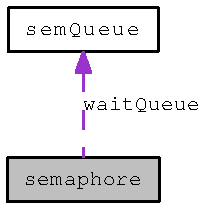
\includegraphics[width=136pt]{structsemaphore__coll__graph}
\end{center}
\end{figure}
\subsection*{Data Fields}
\begin{DoxyCompactItemize}
\item 
\hyperlink{types_8h_a158b5efbc244b8995c439d60c976c818}{key\_\-t} \hyperlink{structsemaphore_a9222a19bf63a4f9775ec6307f10955ac}{semid}
\item 
int \hyperlink{structsemaphore_a6191200d6dbe7f09897db13350a06c61}{semval}
\item 
int \hyperlink{structsemaphore_a89f234133d3efe315836311cbf21c64b}{state}
\item 
\hyperlink{types_8h_ab612a3a4eb0e2ced1e55ecff76260458}{pid\_\-t} \hyperlink{structsemaphore_ab2c2b336eae3da49c4f83d6f44c1fc7b}{sempid}
\item 
\hyperlink{structsem_queue}{semQueue\_\-t} $\ast$ \hyperlink{structsemaphore_aa98d8a188e5b2388de0be4c7c48709fe}{waitQueue}
\end{DoxyCompactItemize}


\subsection{Detailed Description}


Definition at line 17 of file semaphore.c.



\subsection{Field Documentation}
\hypertarget{structsemaphore_a9222a19bf63a4f9775ec6307f10955ac}{
\index{semaphore@{semaphore}!semid@{semid}}
\index{semid@{semid}!semaphore@{semaphore}}
\subsubsection[{semid}]{\setlength{\rightskip}{0pt plus 5cm}{\bf key\_\-t} {\bf semid}}}
\label{structsemaphore_a9222a19bf63a4f9775ec6307f10955ac}


Definition at line 18 of file semaphore.c.

\hypertarget{structsemaphore_ab2c2b336eae3da49c4f83d6f44c1fc7b}{
\index{semaphore@{semaphore}!sempid@{sempid}}
\index{sempid@{sempid}!semaphore@{semaphore}}
\subsubsection[{sempid}]{\setlength{\rightskip}{0pt plus 5cm}{\bf pid\_\-t} {\bf sempid}}}
\label{structsemaphore_ab2c2b336eae3da49c4f83d6f44c1fc7b}


Definition at line 21 of file semaphore.c.

\hypertarget{structsemaphore_a6191200d6dbe7f09897db13350a06c61}{
\index{semaphore@{semaphore}!semval@{semval}}
\index{semval@{semval}!semaphore@{semaphore}}
\subsubsection[{semval}]{\setlength{\rightskip}{0pt plus 5cm}int {\bf semval}}}
\label{structsemaphore_a6191200d6dbe7f09897db13350a06c61}


Definition at line 19 of file semaphore.c.

\hypertarget{structsemaphore_a89f234133d3efe315836311cbf21c64b}{
\index{semaphore@{semaphore}!state@{state}}
\index{state@{state}!semaphore@{semaphore}}
\subsubsection[{state}]{\setlength{\rightskip}{0pt plus 5cm}int {\bf state}}}
\label{structsemaphore_a89f234133d3efe315836311cbf21c64b}


Definition at line 20 of file semaphore.c.

\hypertarget{structsemaphore_aa98d8a188e5b2388de0be4c7c48709fe}{
\index{semaphore@{semaphore}!waitQueue@{waitQueue}}
\index{waitQueue@{waitQueue}!semaphore@{semaphore}}
\subsubsection[{waitQueue}]{\setlength{\rightskip}{0pt plus 5cm}{\bf semQueue\_\-t}$\ast$ {\bf waitQueue}}}
\label{structsemaphore_aa98d8a188e5b2388de0be4c7c48709fe}


Definition at line 22 of file semaphore.c.



The documentation for this struct was generated from the following file:\begin{DoxyCompactItemize}
\item 
src/\hyperlink{semaphore_8c}{semaphore.c}\end{DoxyCompactItemize}

\hypertarget{structsem_queue}{
\section{semQueue Struct Reference}
\label{structsem_queue}\index{semQueue@{semQueue}}
}
\subsection*{Data Fields}
\begin{DoxyCompactItemize}
\item 
\hyperlink{types_8h_ab612a3a4eb0e2ced1e55ecff76260458}{pid\_\-t} \hyperlink{structsem_queue_a851c68a9d8a28e48ed3d9bfc73d9beda}{pids} \mbox{[}MAX\_\-PROCESS\mbox{]}
\item 
int \hyperlink{structsem_queue_a3742955749f912de093848fe1385659d}{actPos}
\item 
int \hyperlink{structsem_queue_a9d456afc79beb2848acfed9c69887f8a}{pidsQty}
\end{DoxyCompactItemize}


\subsection{Detailed Description}


Definition at line 11 of file semaphore.c.



\subsection{Field Documentation}
\hypertarget{structsem_queue_a3742955749f912de093848fe1385659d}{
\index{semQueue@{semQueue}!actPos@{actPos}}
\index{actPos@{actPos}!semQueue@{semQueue}}
\subsubsection[{actPos}]{\setlength{\rightskip}{0pt plus 5cm}int {\bf actPos}}}
\label{structsem_queue_a3742955749f912de093848fe1385659d}


Definition at line 13 of file semaphore.c.

\hypertarget{structsem_queue_a851c68a9d8a28e48ed3d9bfc73d9beda}{
\index{semQueue@{semQueue}!pids@{pids}}
\index{pids@{pids}!semQueue@{semQueue}}
\subsubsection[{pids}]{\setlength{\rightskip}{0pt plus 5cm}{\bf pid\_\-t} {\bf pids}\mbox{[}MAX\_\-PROCESS\mbox{]}}}
\label{structsem_queue_a851c68a9d8a28e48ed3d9bfc73d9beda}


Definition at line 12 of file semaphore.c.

\hypertarget{structsem_queue_a9d456afc79beb2848acfed9c69887f8a}{
\index{semQueue@{semQueue}!pidsQty@{pidsQty}}
\index{pidsQty@{pidsQty}!semQueue@{semQueue}}
\subsubsection[{pidsQty}]{\setlength{\rightskip}{0pt plus 5cm}int {\bf pidsQty}}}
\label{structsem_queue_a9d456afc79beb2848acfed9c69887f8a}


Definition at line 14 of file semaphore.c.



The documentation for this struct was generated from the following file:\begin{DoxyCompactItemize}
\item 
src/\hyperlink{semaphore_8c}{semaphore.c}\end{DoxyCompactItemize}

\hypertarget{structsh_mem}{
\section{shMem Struct Reference}
\label{structsh_mem}\index{shMem@{shMem}}
}


Collaboration diagram for shMem:\nopagebreak
\begin{figure}[H]
\begin{center}
\leavevmode
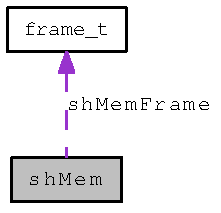
\includegraphics[width=142pt]{structsh_mem__coll__graph}
\end{center}
\end{figure}
\subsection*{Data Fields}
\begin{DoxyCompactItemize}
\item 
int \hyperlink{structsh_mem_ac8807d215d2ee6d9779d76aeb1147430}{shmid}
\item 
\hyperlink{types_8h_a158b5efbc244b8995c439d60c976c818}{key\_\-t} \hyperlink{structsh_mem_ac8861193246fc34d8f29ac9d57b6791a}{key}
\item 
int \hyperlink{structsh_mem_a43617d0cfffcc8578872707c8804b381}{shMemSize}
\item 
\hyperlink{structframe__t}{frame\_\-t} $\ast$ \hyperlink{structsh_mem_a21b32e7678691034a296926c350c2d62}{shMemFrame}
\item 
unsigned int \hyperlink{structsh_mem_af69f25548b68c95b9142a8cea59796bb}{shMemP}
\item 
\hyperlink{types_8h_a158b5efbc244b8995c439d60c976c818}{key\_\-t} \hyperlink{structsh_mem_a9222a19bf63a4f9775ec6307f10955ac}{semid}
\item 
int \hyperlink{structsh_mem_a89f234133d3efe315836311cbf21c64b}{state}
\item 
int \hyperlink{structsh_mem_a720a6e55514a9c4aee4b913a7f871c31}{permFlags}
\item 
int \hyperlink{structsh_mem_aab6ea7924dbc5e67cbf5923d4226ea91}{appnProcessesAmm}
\item 
\hyperlink{types_8h_ab612a3a4eb0e2ced1e55ecff76260458}{pid\_\-t} \hyperlink{structsh_mem_a5bb581de55dfe5f03f5b8b1646a93b38}{appnProcessesPids} \mbox{[}MAX\_\-SHMAPPN\mbox{]}
\end{DoxyCompactItemize}


\subsection{Detailed Description}


Definition at line 16 of file shMemory.c.



\subsection{Field Documentation}
\hypertarget{structsh_mem_aab6ea7924dbc5e67cbf5923d4226ea91}{
\index{shMem@{shMem}!appnProcessesAmm@{appnProcessesAmm}}
\index{appnProcessesAmm@{appnProcessesAmm}!shMem@{shMem}}
\subsubsection[{appnProcessesAmm}]{\setlength{\rightskip}{0pt plus 5cm}int {\bf appnProcessesAmm}}}
\label{structsh_mem_aab6ea7924dbc5e67cbf5923d4226ea91}


Definition at line 25 of file shMemory.c.

\hypertarget{structsh_mem_a5bb581de55dfe5f03f5b8b1646a93b38}{
\index{shMem@{shMem}!appnProcessesPids@{appnProcessesPids}}
\index{appnProcessesPids@{appnProcessesPids}!shMem@{shMem}}
\subsubsection[{appnProcessesPids}]{\setlength{\rightskip}{0pt plus 5cm}{\bf pid\_\-t} {\bf appnProcessesPids}\mbox{[}MAX\_\-SHMAPPN\mbox{]}}}
\label{structsh_mem_a5bb581de55dfe5f03f5b8b1646a93b38}


Definition at line 26 of file shMemory.c.

\hypertarget{structsh_mem_ac8861193246fc34d8f29ac9d57b6791a}{
\index{shMem@{shMem}!key@{key}}
\index{key@{key}!shMem@{shMem}}
\subsubsection[{key}]{\setlength{\rightskip}{0pt plus 5cm}{\bf key\_\-t} {\bf key}}}
\label{structsh_mem_ac8861193246fc34d8f29ac9d57b6791a}


Definition at line 18 of file shMemory.c.

\hypertarget{structsh_mem_a720a6e55514a9c4aee4b913a7f871c31}{
\index{shMem@{shMem}!permFlags@{permFlags}}
\index{permFlags@{permFlags}!shMem@{shMem}}
\subsubsection[{permFlags}]{\setlength{\rightskip}{0pt plus 5cm}int {\bf permFlags}}}
\label{structsh_mem_a720a6e55514a9c4aee4b913a7f871c31}


Definition at line 24 of file shMemory.c.

\hypertarget{structsh_mem_a9222a19bf63a4f9775ec6307f10955ac}{
\index{shMem@{shMem}!semid@{semid}}
\index{semid@{semid}!shMem@{shMem}}
\subsubsection[{semid}]{\setlength{\rightskip}{0pt plus 5cm}{\bf key\_\-t} {\bf semid}}}
\label{structsh_mem_a9222a19bf63a4f9775ec6307f10955ac}


Definition at line 22 of file shMemory.c.

\hypertarget{structsh_mem_a21b32e7678691034a296926c350c2d62}{
\index{shMem@{shMem}!shMemFrame@{shMemFrame}}
\index{shMemFrame@{shMemFrame}!shMem@{shMem}}
\subsubsection[{shMemFrame}]{\setlength{\rightskip}{0pt plus 5cm}{\bf frame\_\-t}$\ast$ {\bf shMemFrame}}}
\label{structsh_mem_a21b32e7678691034a296926c350c2d62}


Definition at line 20 of file shMemory.c.

\hypertarget{structsh_mem_af69f25548b68c95b9142a8cea59796bb}{
\index{shMem@{shMem}!shMemP@{shMemP}}
\index{shMemP@{shMemP}!shMem@{shMem}}
\subsubsection[{shMemP}]{\setlength{\rightskip}{0pt plus 5cm}unsigned int {\bf shMemP}}}
\label{structsh_mem_af69f25548b68c95b9142a8cea59796bb}


Definition at line 21 of file shMemory.c.

\hypertarget{structsh_mem_a43617d0cfffcc8578872707c8804b381}{
\index{shMem@{shMem}!shMemSize@{shMemSize}}
\index{shMemSize@{shMemSize}!shMem@{shMem}}
\subsubsection[{shMemSize}]{\setlength{\rightskip}{0pt plus 5cm}int {\bf shMemSize}}}
\label{structsh_mem_a43617d0cfffcc8578872707c8804b381}


Definition at line 19 of file shMemory.c.

\hypertarget{structsh_mem_ac8807d215d2ee6d9779d76aeb1147430}{
\index{shMem@{shMem}!shmid@{shmid}}
\index{shmid@{shmid}!shMem@{shMem}}
\subsubsection[{shmid}]{\setlength{\rightskip}{0pt plus 5cm}int {\bf shmid}}}
\label{structsh_mem_ac8807d215d2ee6d9779d76aeb1147430}


Definition at line 17 of file shMemory.c.

\hypertarget{structsh_mem_a89f234133d3efe315836311cbf21c64b}{
\index{shMem@{shMem}!state@{state}}
\index{state@{state}!shMem@{shMem}}
\subsubsection[{state}]{\setlength{\rightskip}{0pt plus 5cm}int {\bf state}}}
\label{structsh_mem_a89f234133d3efe315836311cbf21c64b}


Definition at line 23 of file shMemory.c.



The documentation for this struct was generated from the following file:\begin{DoxyCompactItemize}
\item 
src/\hyperlink{sh_memory_8c}{shMemory.c}\end{DoxyCompactItemize}

\hypertarget{structstd_in_t_t_y}{
\section{stdInTTY Struct Reference}
\label{structstd_in_t_t_y}\index{stdInTTY@{stdInTTY}}
}


The tty stdin struct.  




{\ttfamily \#include $<$types.h$>$}

\subsection*{Data Fields}
\begin{DoxyCompactItemize}
\item 
\hyperlink{types_8h_a90ed3c9028a7fa45665d10b5210fa142}{Keycode} $\ast$ \hyperlink{structstd_in_t_t_y_adbc1696a6e5a5d97b6761336fc185945}{stdInBuffer}
\item 
int \hyperlink{structstd_in_t_t_y_ada738b143166d2de18a92ff55801f41b}{writeOffset}
\end{DoxyCompactItemize}


\subsection{Detailed Description}
The tty stdin struct. 

Definition at line 233 of file types.h.



\subsection{Field Documentation}
\hypertarget{structstd_in_t_t_y_adbc1696a6e5a5d97b6761336fc185945}{
\index{stdInTTY@{stdInTTY}!stdInBuffer@{stdInBuffer}}
\index{stdInBuffer@{stdInBuffer}!stdInTTY@{stdInTTY}}
\subsubsection[{stdInBuffer}]{\setlength{\rightskip}{0pt plus 5cm}{\bf Keycode}$\ast$ {\bf stdInBuffer}}}
\label{structstd_in_t_t_y_adbc1696a6e5a5d97b6761336fc185945}


Definition at line 234 of file types.h.

\hypertarget{structstd_in_t_t_y_ada738b143166d2de18a92ff55801f41b}{
\index{stdInTTY@{stdInTTY}!writeOffset@{writeOffset}}
\index{writeOffset@{writeOffset}!stdInTTY@{stdInTTY}}
\subsubsection[{writeOffset}]{\setlength{\rightskip}{0pt plus 5cm}int {\bf writeOffset}}}
\label{structstd_in_t_t_y_ada738b143166d2de18a92ff55801f41b}


Definition at line 235 of file types.h.



The documentation for this struct was generated from the following file:\begin{DoxyCompactItemize}
\item 
inc/\hyperlink{types_8h}{types.h}\end{DoxyCompactItemize}

\hypertarget{structstd_out_t_t_y}{
\section{stdOutTTY Struct Reference}
\label{structstd_out_t_t_y}\index{stdOutTTY@{stdOutTTY}}
}


The tty stdout struct.  




{\ttfamily \#include $<$types.h$>$}

\subsection*{Data Fields}
\begin{DoxyCompactItemize}
\item 
\hyperlink{types_8h_a90ed3c9028a7fa45665d10b5210fa142}{Keycode} $\ast$ \hyperlink{structstd_out_t_t_y_aef253d03c960d4ee76bc0f0f84236f8b}{stdOutBuffer}
\item 
\hyperlink{types_8h_a90ed3c9028a7fa45665d10b5210fa142}{Keycode} $\ast$ \hyperlink{structstd_out_t_t_y_a07f2fe2975e6c3ee1e728566ec50cfab}{begin}
\item 
\hyperlink{types_8h_a90ed3c9028a7fa45665d10b5210fa142}{Keycode} $\ast$ \hyperlink{structstd_out_t_t_y_a69c1bb32d9b06f32161aff7f1c822c97}{end}
\end{DoxyCompactItemize}


\subsection{Detailed Description}
The tty stdout struct. 

Definition at line 242 of file types.h.



\subsection{Field Documentation}
\hypertarget{structstd_out_t_t_y_a07f2fe2975e6c3ee1e728566ec50cfab}{
\index{stdOutTTY@{stdOutTTY}!begin@{begin}}
\index{begin@{begin}!stdOutTTY@{stdOutTTY}}
\subsubsection[{begin}]{\setlength{\rightskip}{0pt plus 5cm}{\bf Keycode}$\ast$ {\bf begin}}}
\label{structstd_out_t_t_y_a07f2fe2975e6c3ee1e728566ec50cfab}


Definition at line 244 of file types.h.

\hypertarget{structstd_out_t_t_y_a69c1bb32d9b06f32161aff7f1c822c97}{
\index{stdOutTTY@{stdOutTTY}!end@{end}}
\index{end@{end}!stdOutTTY@{stdOutTTY}}
\subsubsection[{end}]{\setlength{\rightskip}{0pt plus 5cm}{\bf Keycode}$\ast$ {\bf end}}}
\label{structstd_out_t_t_y_a69c1bb32d9b06f32161aff7f1c822c97}


Definition at line 245 of file types.h.

\hypertarget{structstd_out_t_t_y_aef253d03c960d4ee76bc0f0f84236f8b}{
\index{stdOutTTY@{stdOutTTY}!stdOutBuffer@{stdOutBuffer}}
\index{stdOutBuffer@{stdOutBuffer}!stdOutTTY@{stdOutTTY}}
\subsubsection[{stdOutBuffer}]{\setlength{\rightskip}{0pt plus 5cm}{\bf Keycode}$\ast$ {\bf stdOutBuffer}}}
\label{structstd_out_t_t_y_aef253d03c960d4ee76bc0f0f84236f8b}


Definition at line 243 of file types.h.



The documentation for this struct was generated from the following file:\begin{DoxyCompactItemize}
\item 
inc/\hyperlink{types_8h}{types.h}\end{DoxyCompactItemize}

\hypertarget{structsys_t_t_y}{
\section{sysTTY Struct Reference}
\label{structsys_t_t_y}\index{sysTTY@{sysTTY}}
}


The tty system struct.  




{\ttfamily \#include $<$types.h$>$}



Collaboration diagram for sysTTY:\nopagebreak
\begin{figure}[H]
\begin{center}
\leavevmode
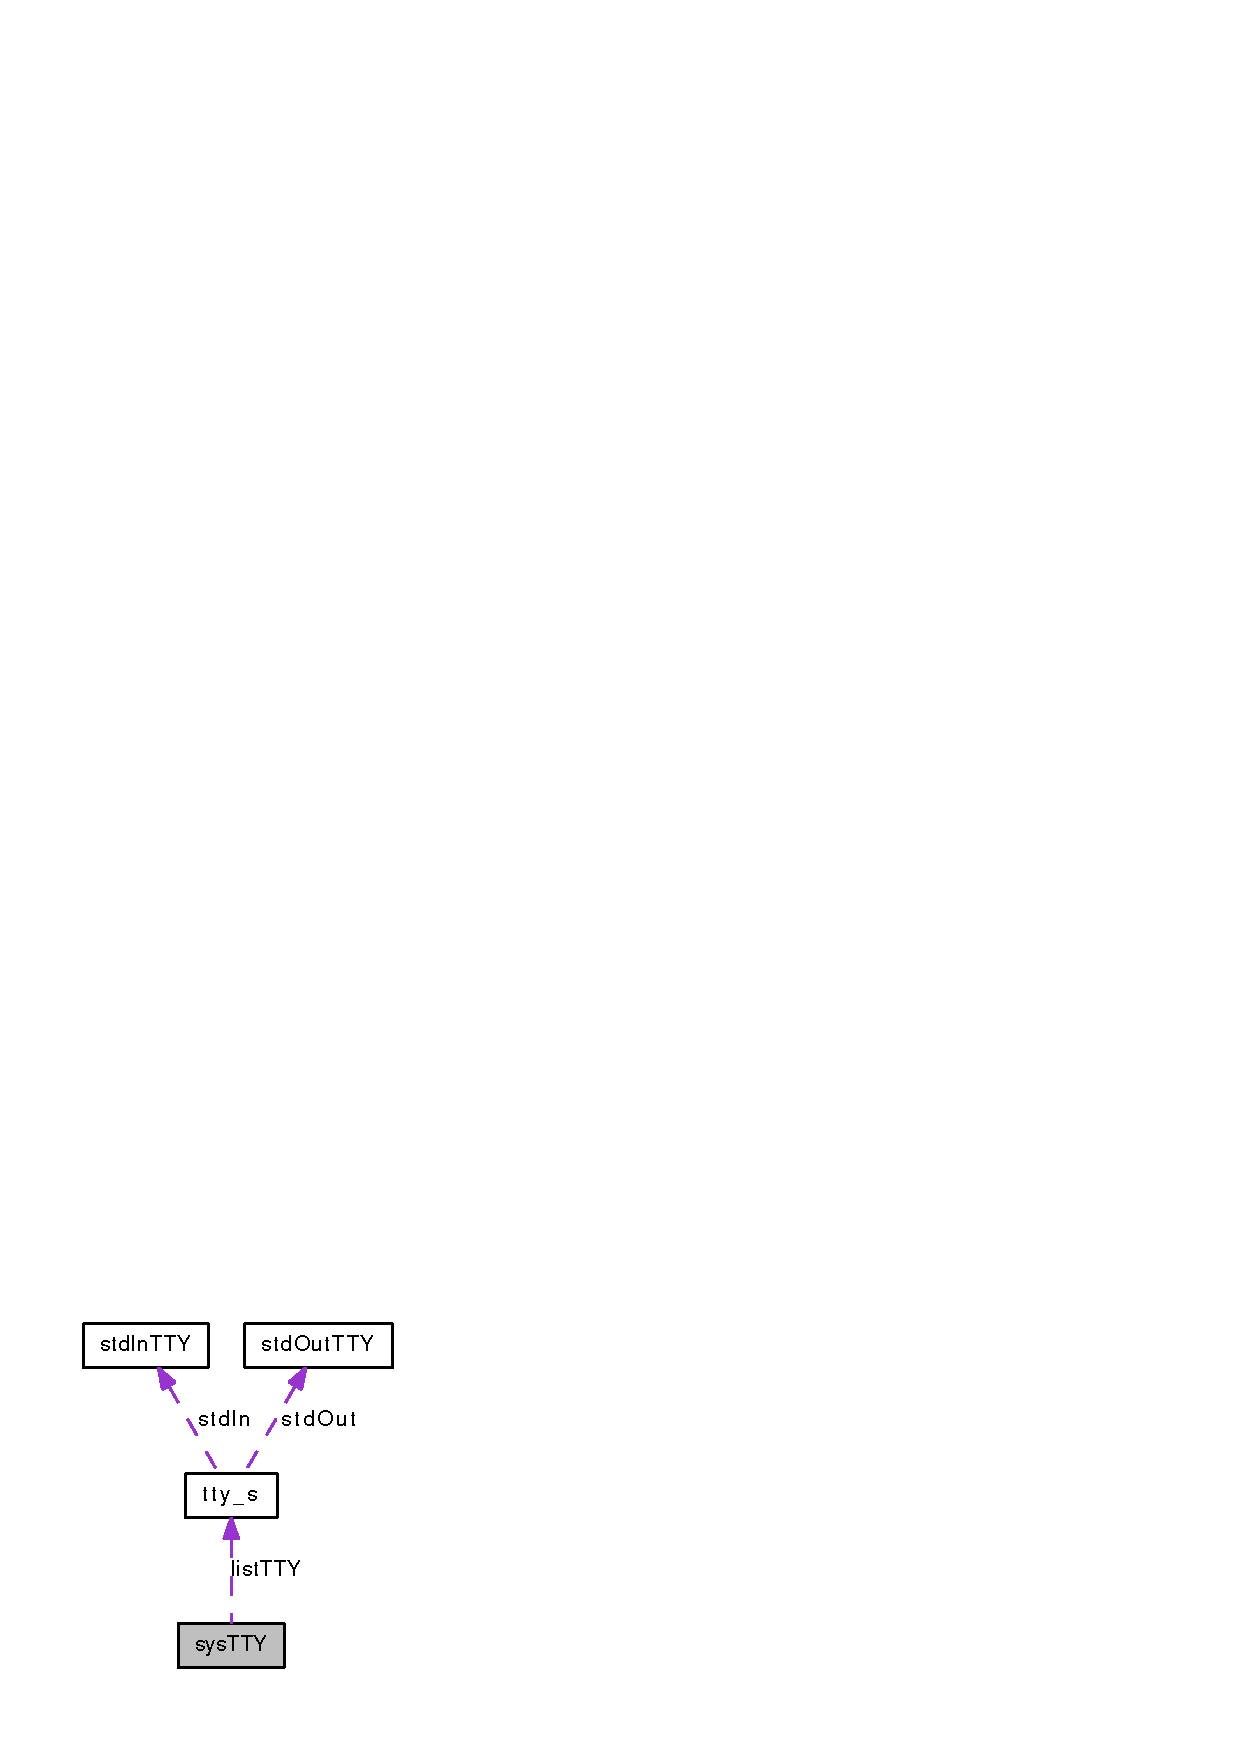
\includegraphics[width=192pt]{structsys_t_t_y__coll__graph}
\end{center}
\end{figure}
\subsection*{Data Fields}
\begin{DoxyCompactItemize}
\item 
int \hyperlink{structsys_t_t_y_a0bc680aada6c6392e4613573f212438b}{qtyTTY}
\item 
\hyperlink{structtty__s}{tty\_\-s} $\ast$ \hyperlink{structsys_t_t_y_a35ea653106226d6fe2191f4f8a203d67}{listTTY} \mbox{[}MAX\_\-TTY\mbox{]}
\item 
\hyperlink{types_8h_a10bbb7176245baeab9f398547c410779}{tty\_\-t} \hyperlink{structsys_t_t_y_ad4f84dd55c369a7bd7d9f562fc76662f}{focusTTY}
\end{DoxyCompactItemize}


\subsection{Detailed Description}
The tty system struct. 

Definition at line 270 of file types.h.



\subsection{Field Documentation}
\hypertarget{structsys_t_t_y_ad4f84dd55c369a7bd7d9f562fc76662f}{
\index{sysTTY@{sysTTY}!focusTTY@{focusTTY}}
\index{focusTTY@{focusTTY}!sysTTY@{sysTTY}}
\subsubsection[{focusTTY}]{\setlength{\rightskip}{0pt plus 5cm}{\bf tty\_\-t} {\bf focusTTY}}}
\label{structsys_t_t_y_ad4f84dd55c369a7bd7d9f562fc76662f}


Definition at line 273 of file types.h.

\hypertarget{structsys_t_t_y_a35ea653106226d6fe2191f4f8a203d67}{
\index{sysTTY@{sysTTY}!listTTY@{listTTY}}
\index{listTTY@{listTTY}!sysTTY@{sysTTY}}
\subsubsection[{listTTY}]{\setlength{\rightskip}{0pt plus 5cm}{\bf tty\_\-s}$\ast$ {\bf listTTY}\mbox{[}MAX\_\-TTY\mbox{]}}}
\label{structsys_t_t_y_a35ea653106226d6fe2191f4f8a203d67}


Definition at line 272 of file types.h.

\hypertarget{structsys_t_t_y_a0bc680aada6c6392e4613573f212438b}{
\index{sysTTY@{sysTTY}!qtyTTY@{qtyTTY}}
\index{qtyTTY@{qtyTTY}!sysTTY@{sysTTY}}
\subsubsection[{qtyTTY}]{\setlength{\rightskip}{0pt plus 5cm}int {\bf qtyTTY}}}
\label{structsys_t_t_y_a0bc680aada6c6392e4613573f212438b}


Definition at line 271 of file types.h.



The documentation for this struct was generated from the following file:\begin{DoxyCompactItemize}
\item 
inc/\hyperlink{types_8h}{types.h}\end{DoxyCompactItemize}

\hypertarget{structtty__s}{
\section{tty\_\-s Struct Reference}
\label{structtty__s}\index{tty\_\-s@{tty\_\-s}}
}


The \hyperlink{structtty__s}{tty\_\-s} struct.  




{\ttfamily \#include $<$types.h$>$}



Collaboration diagram for tty\_\-s:\nopagebreak
\begin{figure}[H]
\begin{center}
\leavevmode
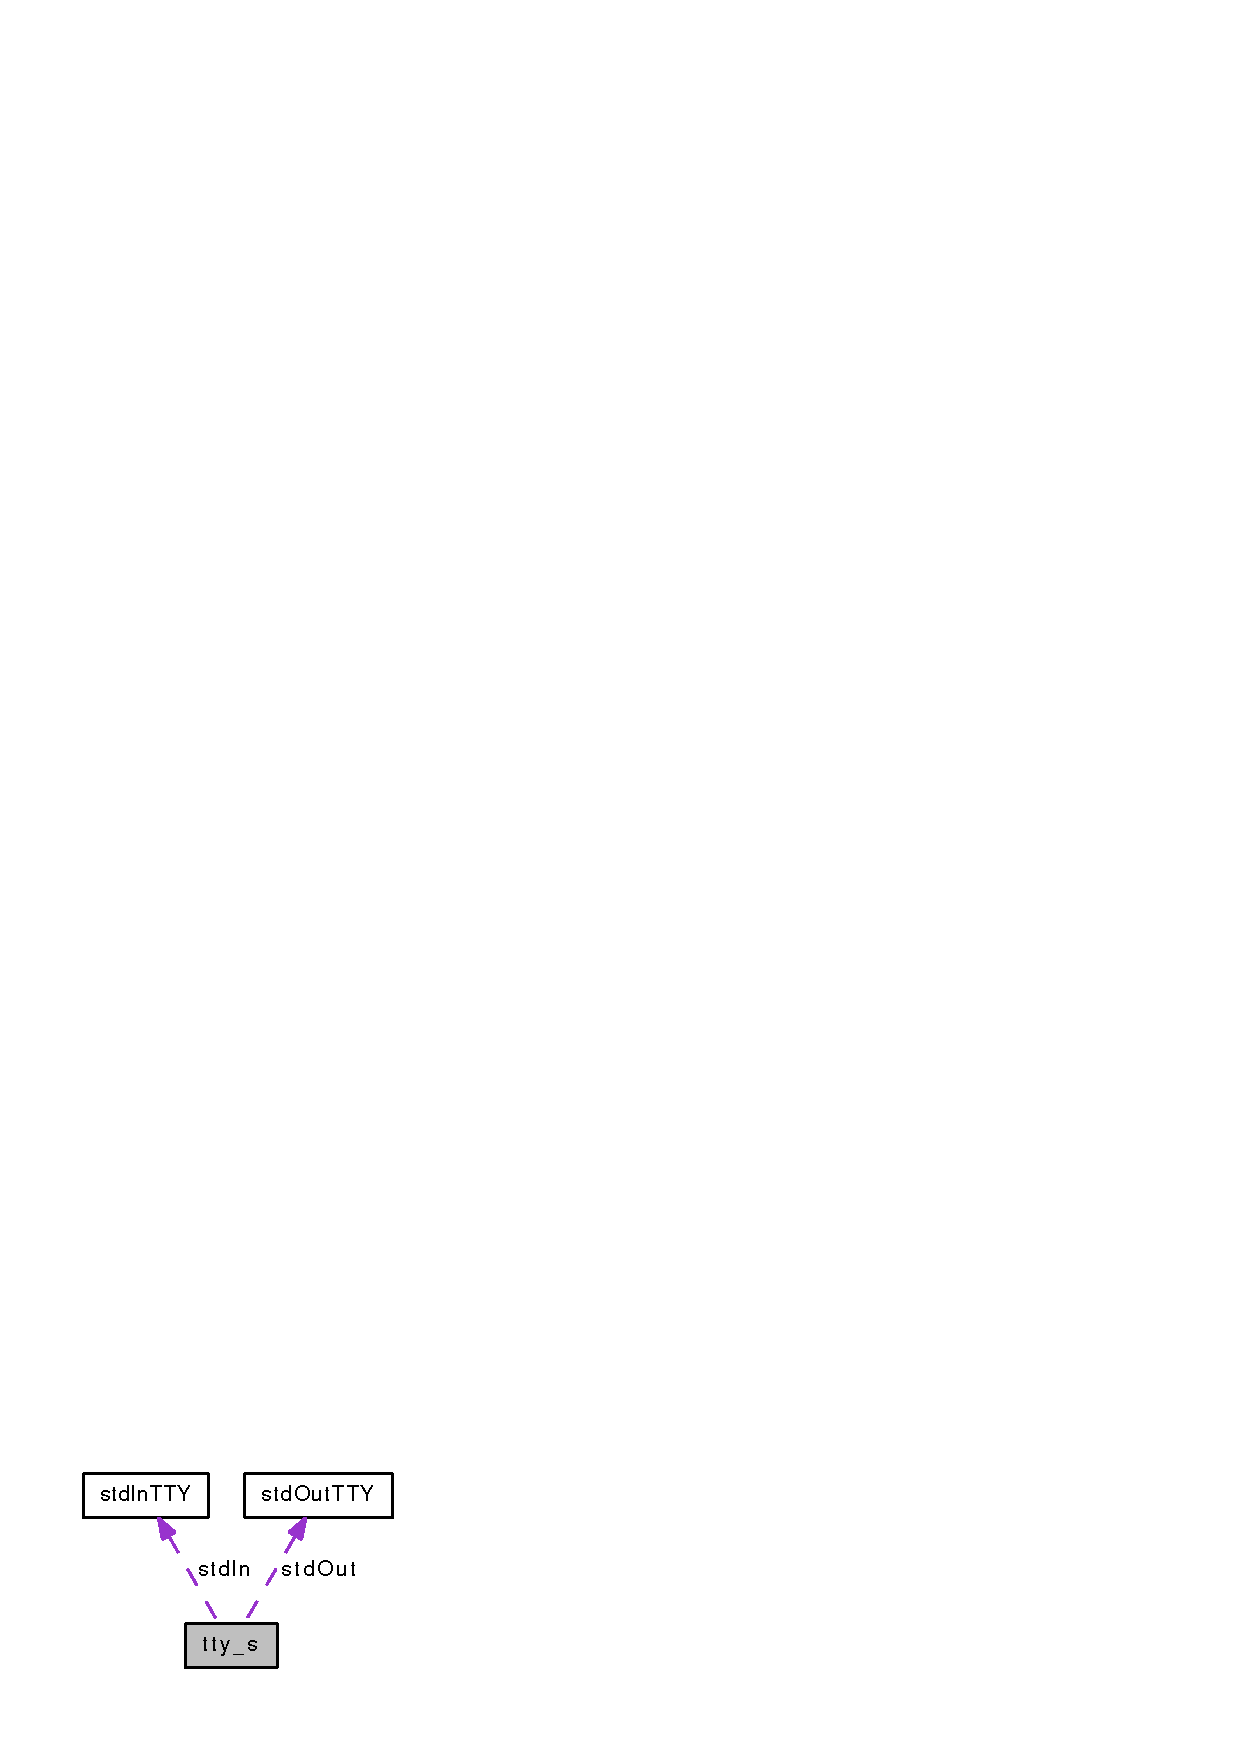
\includegraphics[width=192pt]{structtty__s__coll__graph}
\end{center}
\end{figure}
\subsection*{Data Fields}
\begin{DoxyCompactItemize}
\item 
\hyperlink{types_8h_a10bbb7176245baeab9f398547c410779}{tty\_\-t} \hyperlink{structtty__s_a7bdcbca143d0773edef7d01762d42aff}{ttyId}
\item 
\hyperlink{structstd_in_t_t_y}{stdInTTY} $\ast$ \hyperlink{structtty__s_a44c2fc56a32fd5125ebc51b6b2c0e178}{stdIn}
\item 
\hyperlink{structstd_out_t_t_y}{stdOutTTY} $\ast$ \hyperlink{structtty__s_a0651a2e4ac304fdc5837a8eb0b0bd166}{stdOut}
\item 
int \hyperlink{structtty__s_a5be2ba5c5e17899443300974060fe13f}{hasScrolled}
\item 
\hyperlink{types_8h_ab612a3a4eb0e2ced1e55ecff76260458}{pid\_\-t} \hyperlink{structtty__s_afefb5a7d2161ce434bcc2bbb358d5b0b}{focusProcess}
\item 
int \hyperlink{structtty__s_a3a1ce6ba5935d1763d5b04f50fee62f7}{writePointer}
\item 
int \hyperlink{structtty__s_ae1216492f5b395a931efcab6127d0160}{writeCol}
\item 
int \hyperlink{structtty__s_a0bd76a596e01d0e7b4775aab29dcf425}{writeRow}
\item 
int \hyperlink{structtty__s_aa0a6145a711115035caf96d6d1c7d9fb}{readPointer}
\item 
int \hyperlink{structtty__s_a38beda239dc9e9eb6f58cc2e818fbaa6}{readCol}
\item 
int \hyperlink{structtty__s_a0aef55ec53e97b2ad384eb814d316e9b}{readRow}
\end{DoxyCompactItemize}


\subsection{Detailed Description}
The \hyperlink{structtty__s}{tty\_\-s} struct. 

Definition at line 252 of file types.h.



\subsection{Field Documentation}
\hypertarget{structtty__s_afefb5a7d2161ce434bcc2bbb358d5b0b}{
\index{tty\_\-s@{tty\_\-s}!focusProcess@{focusProcess}}
\index{focusProcess@{focusProcess}!tty_s@{tty\_\-s}}
\subsubsection[{focusProcess}]{\setlength{\rightskip}{0pt plus 5cm}{\bf pid\_\-t} {\bf focusProcess}}}
\label{structtty__s_afefb5a7d2161ce434bcc2bbb358d5b0b}


Definition at line 257 of file types.h.

\hypertarget{structtty__s_a5be2ba5c5e17899443300974060fe13f}{
\index{tty\_\-s@{tty\_\-s}!hasScrolled@{hasScrolled}}
\index{hasScrolled@{hasScrolled}!tty_s@{tty\_\-s}}
\subsubsection[{hasScrolled}]{\setlength{\rightskip}{0pt plus 5cm}int {\bf hasScrolled}}}
\label{structtty__s_a5be2ba5c5e17899443300974060fe13f}


Definition at line 256 of file types.h.

\hypertarget{structtty__s_a38beda239dc9e9eb6f58cc2e818fbaa6}{
\index{tty\_\-s@{tty\_\-s}!readCol@{readCol}}
\index{readCol@{readCol}!tty_s@{tty\_\-s}}
\subsubsection[{readCol}]{\setlength{\rightskip}{0pt plus 5cm}int {\bf readCol}}}
\label{structtty__s_a38beda239dc9e9eb6f58cc2e818fbaa6}


Definition at line 262 of file types.h.

\hypertarget{structtty__s_aa0a6145a711115035caf96d6d1c7d9fb}{
\index{tty\_\-s@{tty\_\-s}!readPointer@{readPointer}}
\index{readPointer@{readPointer}!tty_s@{tty\_\-s}}
\subsubsection[{readPointer}]{\setlength{\rightskip}{0pt plus 5cm}int {\bf readPointer}}}
\label{structtty__s_aa0a6145a711115035caf96d6d1c7d9fb}


Definition at line 261 of file types.h.

\hypertarget{structtty__s_a0aef55ec53e97b2ad384eb814d316e9b}{
\index{tty\_\-s@{tty\_\-s}!readRow@{readRow}}
\index{readRow@{readRow}!tty_s@{tty\_\-s}}
\subsubsection[{readRow}]{\setlength{\rightskip}{0pt plus 5cm}int {\bf readRow}}}
\label{structtty__s_a0aef55ec53e97b2ad384eb814d316e9b}


Definition at line 263 of file types.h.

\hypertarget{structtty__s_a44c2fc56a32fd5125ebc51b6b2c0e178}{
\index{tty\_\-s@{tty\_\-s}!stdIn@{stdIn}}
\index{stdIn@{stdIn}!tty_s@{tty\_\-s}}
\subsubsection[{stdIn}]{\setlength{\rightskip}{0pt plus 5cm}{\bf stdInTTY}$\ast$ {\bf stdIn}}}
\label{structtty__s_a44c2fc56a32fd5125ebc51b6b2c0e178}


Definition at line 254 of file types.h.

\hypertarget{structtty__s_a0651a2e4ac304fdc5837a8eb0b0bd166}{
\index{tty\_\-s@{tty\_\-s}!stdOut@{stdOut}}
\index{stdOut@{stdOut}!tty_s@{tty\_\-s}}
\subsubsection[{stdOut}]{\setlength{\rightskip}{0pt plus 5cm}{\bf stdOutTTY}$\ast$ {\bf stdOut}}}
\label{structtty__s_a0651a2e4ac304fdc5837a8eb0b0bd166}


Definition at line 255 of file types.h.

\hypertarget{structtty__s_a7bdcbca143d0773edef7d01762d42aff}{
\index{tty\_\-s@{tty\_\-s}!ttyId@{ttyId}}
\index{ttyId@{ttyId}!tty_s@{tty\_\-s}}
\subsubsection[{ttyId}]{\setlength{\rightskip}{0pt plus 5cm}{\bf tty\_\-t} {\bf ttyId}}}
\label{structtty__s_a7bdcbca143d0773edef7d01762d42aff}


Definition at line 253 of file types.h.

\hypertarget{structtty__s_ae1216492f5b395a931efcab6127d0160}{
\index{tty\_\-s@{tty\_\-s}!writeCol@{writeCol}}
\index{writeCol@{writeCol}!tty_s@{tty\_\-s}}
\subsubsection[{writeCol}]{\setlength{\rightskip}{0pt plus 5cm}int {\bf writeCol}}}
\label{structtty__s_ae1216492f5b395a931efcab6127d0160}


Definition at line 259 of file types.h.

\hypertarget{structtty__s_a3a1ce6ba5935d1763d5b04f50fee62f7}{
\index{tty\_\-s@{tty\_\-s}!writePointer@{writePointer}}
\index{writePointer@{writePointer}!tty_s@{tty\_\-s}}
\subsubsection[{writePointer}]{\setlength{\rightskip}{0pt plus 5cm}int {\bf writePointer}}}
\label{structtty__s_a3a1ce6ba5935d1763d5b04f50fee62f7}


Definition at line 258 of file types.h.

\hypertarget{structtty__s_a0bd76a596e01d0e7b4775aab29dcf425}{
\index{tty\_\-s@{tty\_\-s}!writeRow@{writeRow}}
\index{writeRow@{writeRow}!tty_s@{tty\_\-s}}
\subsubsection[{writeRow}]{\setlength{\rightskip}{0pt plus 5cm}int {\bf writeRow}}}
\label{structtty__s_a0bd76a596e01d0e7b4775aab29dcf425}


Definition at line 260 of file types.h.



The documentation for this struct was generated from the following file:\begin{DoxyCompactItemize}
\item 
inc/\hyperlink{types_8h}{types.h}\end{DoxyCompactItemize}

\chapter{File Documentation}
\hypertarget{bin_8h}{
\section{inc/bin.h File Reference}
\label{bin_8h}\index{inc/bin.h@{inc/bin.h}}
}


All the OS processes.  


{\ttfamily \#include \char`\"{}sysProcess.h\char`\"{}}\par
{\ttfamily \#include \char`\"{}types.h\char`\"{}}\par
{\ttfamily \#include \char`\"{}keyboard\_\-buffer.h\char`\"{}}\par
{\ttfamily \#include \char`\"{}sysProcess.h\char`\"{}}\par
{\ttfamily \#include \char`\"{}string.h\char`\"{}}\par
{\ttfamily \#include \char`\"{}syscall.h\char`\"{}}\par
{\ttfamily \#include \char`\"{}memModule.h\char`\"{}}\par
{\ttfamily \#include \char`\"{}process.h\char`\"{}}\par
{\ttfamily \#include \char`\"{}video\_\-driver.h\char`\"{}}\par
{\ttfamily \#include \char`\"{}kasm.h\char`\"{}}\par
{\ttfamily \#include \char`\"{}ttys.h\char`\"{}}\par
{\ttfamily \#include \char`\"{}unistd.h\char`\"{}}\par
{\ttfamily \#include \char`\"{}sysMalloc.h\char`\"{}}\par
{\ttfamily \#include \char`\"{}stdio.h\char`\"{}}\par
{\ttfamily \#include \char`\"{}schedule.h\char`\"{}}\par
{\ttfamily \#include \char`\"{}kMalloc.h\char`\"{}}\par
{\ttfamily \#include \char`\"{}shell.h\char`\"{}}\par
{\ttfamily \#include \char`\"{}io.h\char`\"{}}\par
{\ttfamily \#include \char`\"{}colors.h\char`\"{}}\par
{\ttfamily \#include \char`\"{}uMalloc.h\char`\"{}}\par
{\ttfamily \#include \char`\"{}semaphore.h\char`\"{}}\par
{\ttfamily \#include \char`\"{}rand.h\char`\"{}}\par
Include dependency graph for bin.h:\nopagebreak
\begin{figure}[H]
\begin{center}
\leavevmode
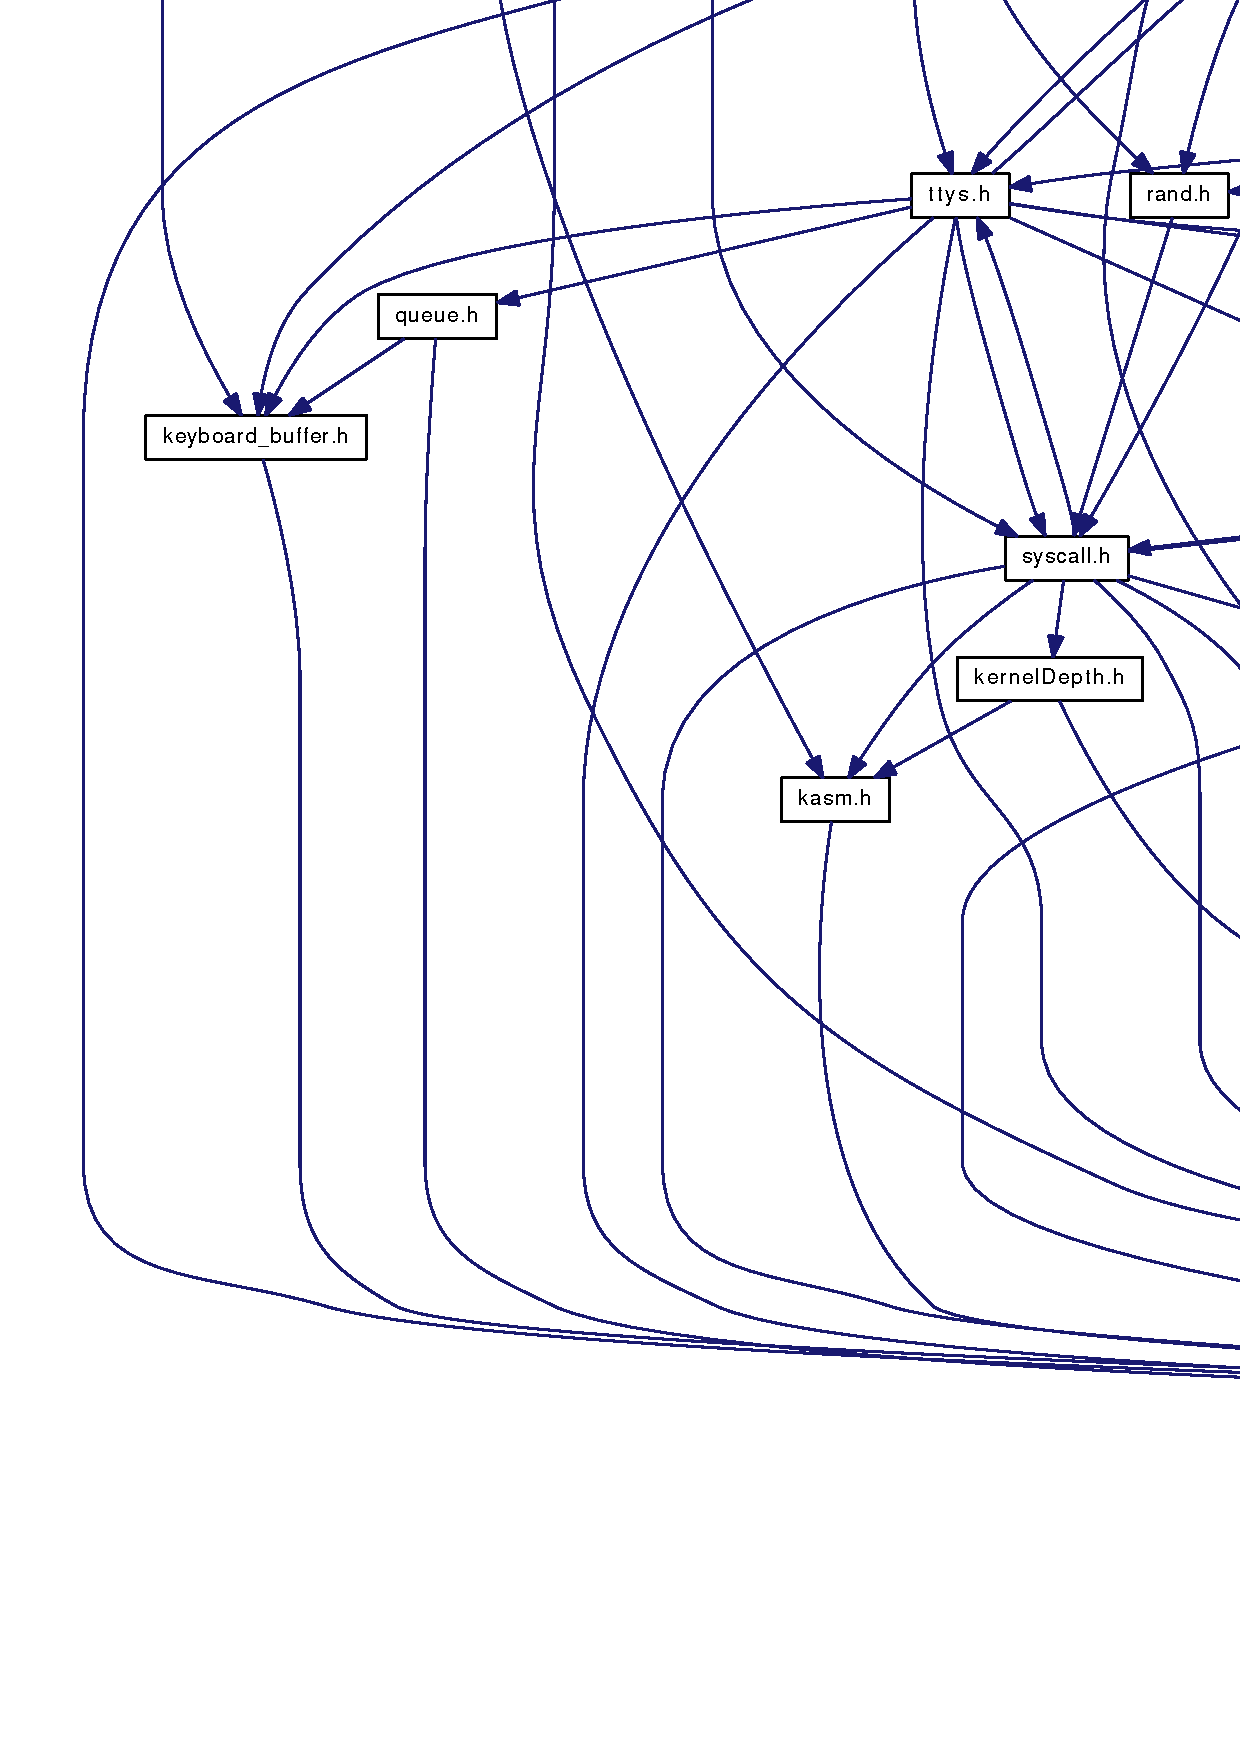
\includegraphics[width=420pt]{bin_8h__incl}
\end{center}
\end{figure}
This graph shows which files directly or indirectly include this file:\nopagebreak
\begin{figure}[H]
\begin{center}
\leavevmode
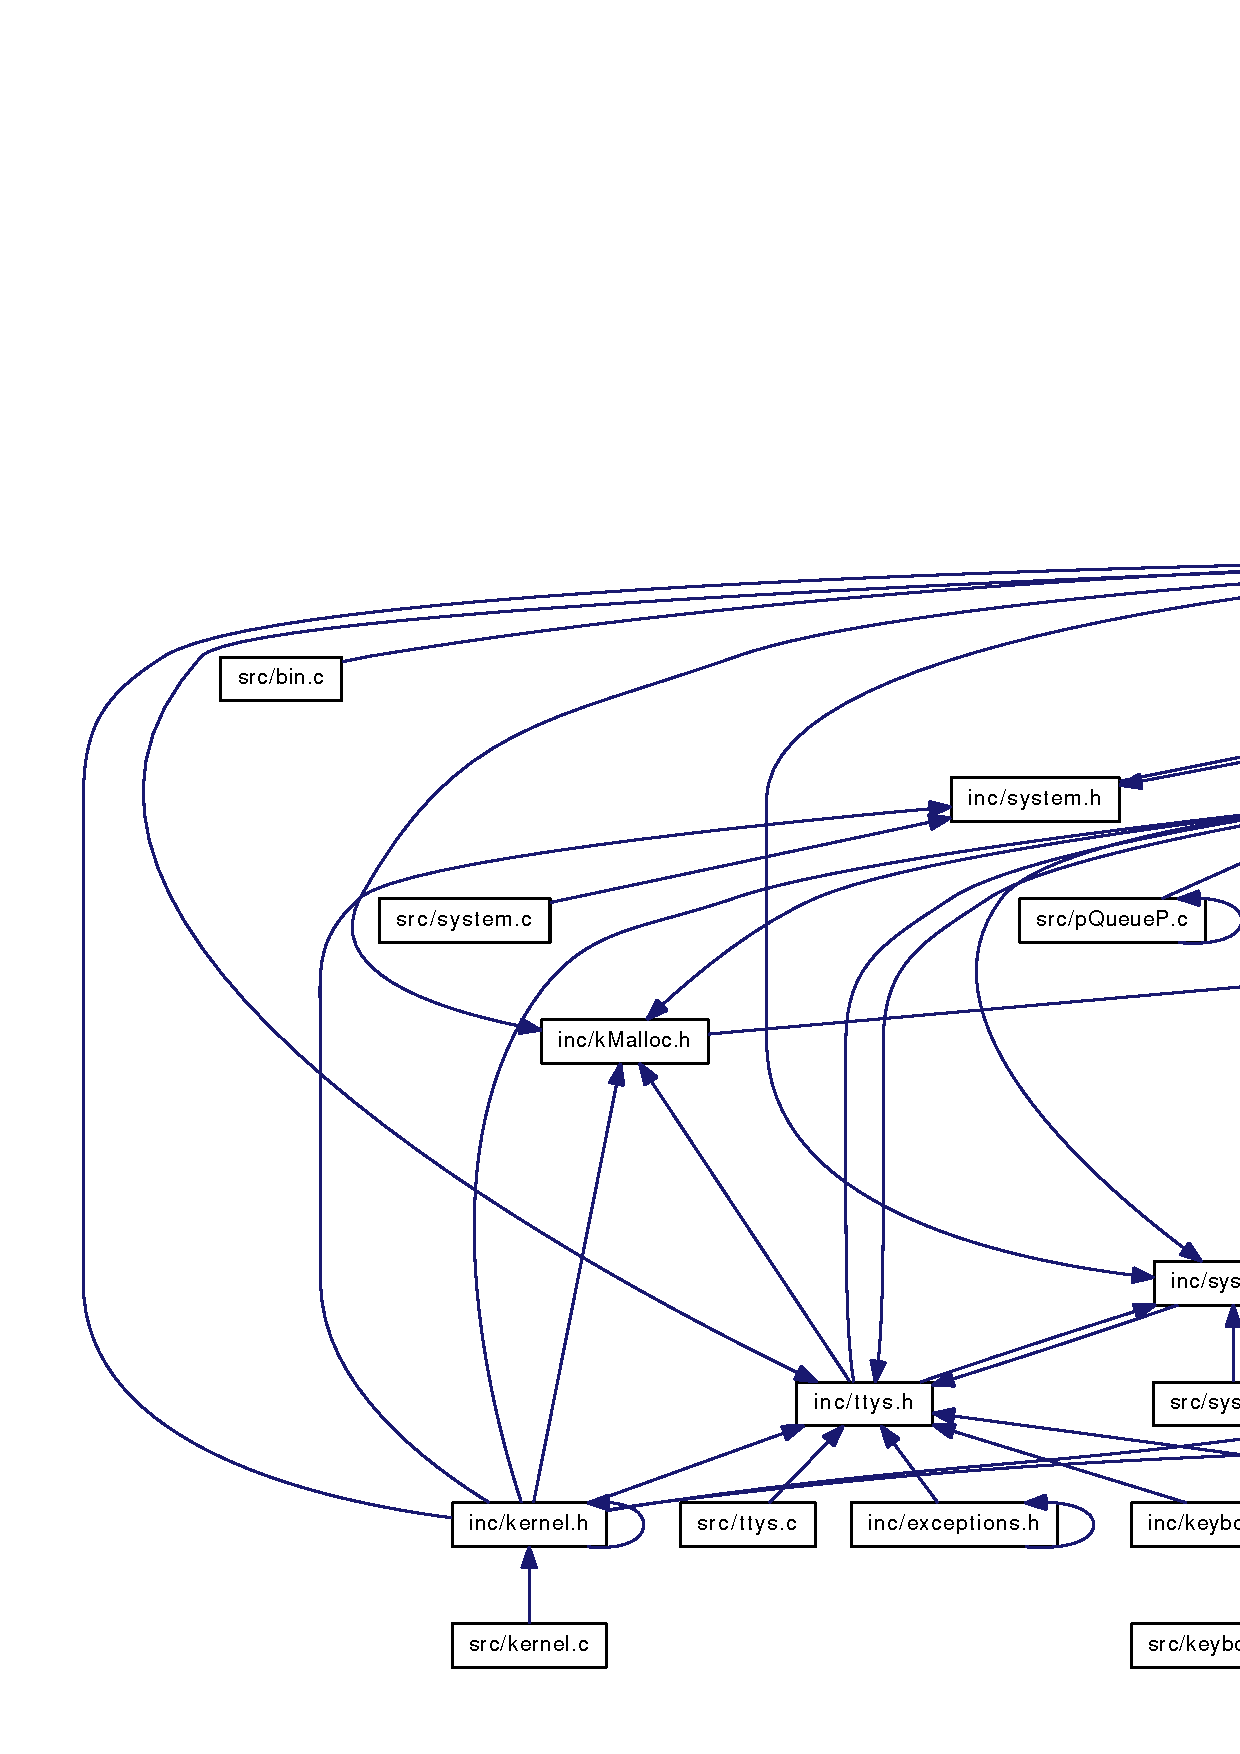
\includegraphics[width=420pt]{bin_8h__dep__incl}
\end{center}
\end{figure}
\subsection*{Functions}
\begin{DoxyCompactItemize}
\item 
void \hyperlink{bin_8h_a5bfde7b5020b14bdcb1c9269ab308dc5}{init} (void $\ast$args)
\begin{DoxyCompactList}\small\item\em This functions initialize the welcome process, all the shells and goodbye process. If you kill the process init the system will be rebooted. \item\end{DoxyCompactList}\item 
void \hyperlink{bin_8h_a9795fbee9531f56aeda1376bf9934506}{top} (char $\ast$args)
\begin{DoxyCompactList}\small\item\em This function show what percentage of the microprocessor it is using each process. When you write the command top in the shell, the process top will be created. \item\end{DoxyCompactList}\item 
void \hyperlink{bin_8h_a236e454e493fc9b262f746305660a2eb}{welcome} ()
\begin{DoxyCompactList}\small\item\em This function just prints the welcome message to Flying-\/High OS. \item\end{DoxyCompactList}\item 
void \hyperlink{bin_8h_ae2338f2b60de8c59eaa31a6a285c1fc0}{goodbye} ()
\begin{DoxyCompactList}\small\item\em This function just says goodbye and reboots the system. \item\end{DoxyCompactList}\item 
void \hyperlink{bin_8h_a8d6f8ce896cba69a844650449479ead1}{printA} ()
\begin{DoxyCompactList}\small\item\em This function prints infinite A letters. \item\end{DoxyCompactList}\item 
void \hyperlink{bin_8h_a5964c5b2b75cb7dc3c7648afe535fd03}{printB} ()
\begin{DoxyCompactList}\small\item\em This functions prints infinite A letters. \item\end{DoxyCompactList}\item 
void \hyperlink{bin_8h_a91d6348b48c15f044abee99da6fec6bd}{nothing} ()
\begin{DoxyCompactList}\small\item\em This function only consumes the microprocessor. \item\end{DoxyCompactList}\item 
void \hyperlink{bin_8h_ab8d39c86e0f803f0816e787e36c99bd1}{pageFault} ()
\begin{DoxyCompactList}\small\item\em This function generates a page fault exception. \item\end{DoxyCompactList}\end{DoxyCompactItemize}


\subsection{Detailed Description}
All the OS processes. \begin{DoxyAuthor}{Author}
Luciano Zemin, Nicolás Magni, Nicolás Purita 
\end{DoxyAuthor}


Definition in file \hyperlink{bin_8h_source}{bin.h}.



\subsection{Function Documentation}
\hypertarget{bin_8h_ae2338f2b60de8c59eaa31a6a285c1fc0}{
\index{bin.h@{bin.h}!goodbye@{goodbye}}
\index{goodbye@{goodbye}!bin.h@{bin.h}}
\subsubsection[{goodbye}]{\setlength{\rightskip}{0pt plus 5cm}void goodbye ()}}
\label{bin_8h_ae2338f2b60de8c59eaa31a6a285c1fc0}


This function just says goodbye and reboots the system. 

Use: 
\begin{DoxyCode}
                        createProcess("goodbye", (void(*)(void *))goodbye, NULL, 
      FOREGROUND);
\end{DoxyCode}


\begin{DoxySeeAlso}{See also}

\end{DoxySeeAlso}


Definition at line 260 of file bin.c.



Here is the call graph for this function:\nopagebreak
\begin{figure}[H]
\begin{center}
\leavevmode
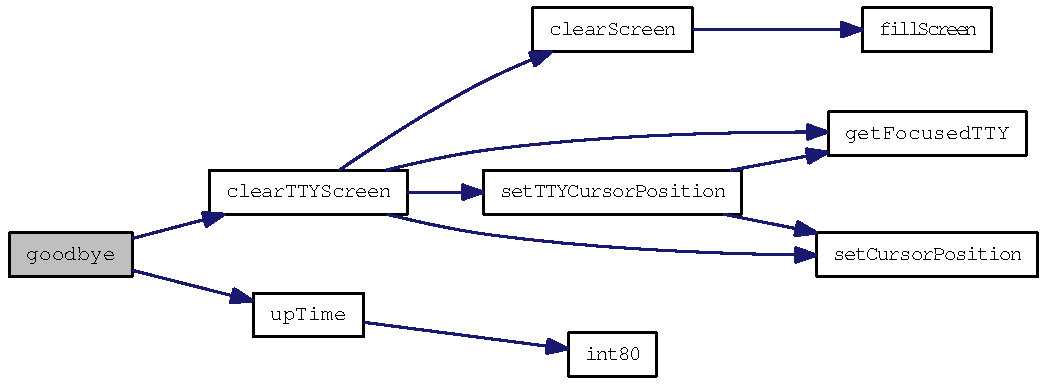
\includegraphics[width=269pt]{bin_8h_ae2338f2b60de8c59eaa31a6a285c1fc0_cgraph}
\end{center}
\end{figure}




Here is the caller graph for this function:\nopagebreak
\begin{figure}[H]
\begin{center}
\leavevmode
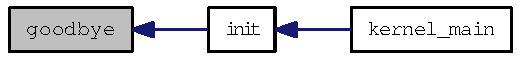
\includegraphics[width=143pt]{bin_8h_ae2338f2b60de8c59eaa31a6a285c1fc0_icgraph}
\end{center}
\end{figure}


\hypertarget{bin_8h_a5bfde7b5020b14bdcb1c9269ab308dc5}{
\index{bin.h@{bin.h}!init@{init}}
\index{init@{init}!bin.h@{bin.h}}
\subsubsection[{init}]{\setlength{\rightskip}{0pt plus 5cm}void init (void $\ast$ {\em args})}}
\label{bin_8h_a5bfde7b5020b14bdcb1c9269ab308dc5}


This functions initialize the welcome process, all the shells and goodbye process. If you kill the process init the system will be rebooted. 


\begin{DoxyParams}{Parameters}
\item[{\em args}]\end{DoxyParams}
Use: 
\begin{DoxyCode}
                        initMultitasker(init);
\end{DoxyCode}
 

Definition at line 14 of file bin.c.



Here is the call graph for this function:\nopagebreak
\begin{figure}[H]
\begin{center}
\leavevmode
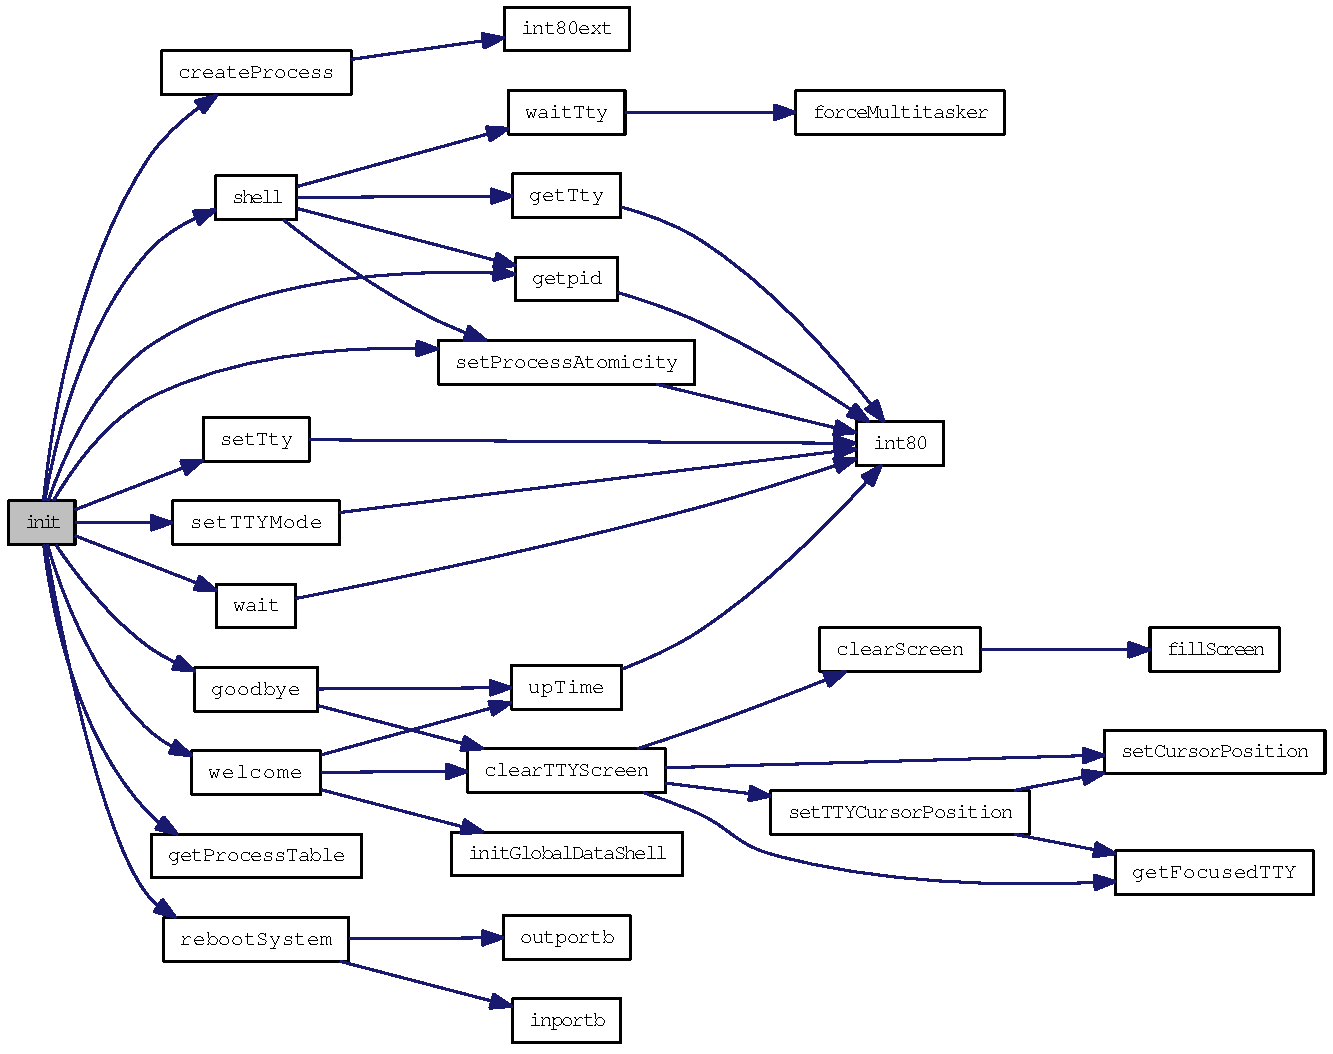
\includegraphics[width=338pt]{bin_8h_a5bfde7b5020b14bdcb1c9269ab308dc5_cgraph}
\end{center}
\end{figure}




Here is the caller graph for this function:\nopagebreak
\begin{figure}[H]
\begin{center}
\leavevmode
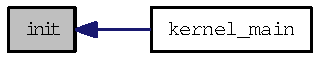
\includegraphics[width=95pt]{bin_8h_a5bfde7b5020b14bdcb1c9269ab308dc5_icgraph}
\end{center}
\end{figure}


\hypertarget{bin_8h_a91d6348b48c15f044abee99da6fec6bd}{
\index{bin.h@{bin.h}!nothing@{nothing}}
\index{nothing@{nothing}!bin.h@{bin.h}}
\subsubsection[{nothing}]{\setlength{\rightskip}{0pt plus 5cm}void nothing ()}}
\label{bin_8h_a91d6348b48c15f044abee99da6fec6bd}


This function only consumes the microprocessor. 

Use: 
\begin{DoxyCode}
                        createProcess("nothing", (void(*)(void *))nothing, NULL, 
      FOREGROUND)
\end{DoxyCode}


\begin{DoxySeeAlso}{See also}

\end{DoxySeeAlso}


Definition at line 308 of file bin.c.

\hypertarget{bin_8h_ab8d39c86e0f803f0816e787e36c99bd1}{
\index{bin.h@{bin.h}!pageFault@{pageFault}}
\index{pageFault@{pageFault}!bin.h@{bin.h}}
\subsubsection[{pageFault}]{\setlength{\rightskip}{0pt plus 5cm}void pageFault ()}}
\label{bin_8h_ab8d39c86e0f803f0816e787e36c99bd1}


This function generates a page fault exception. 

Use: 
\begin{DoxyCode}
                        createProcess("pageFault", (void(*)(void *))pageFault, 
      NULL, FOREGROUND)
\end{DoxyCode}


\begin{DoxySeeAlso}{See also}

\end{DoxySeeAlso}


Definition at line 317 of file bin.c.



Here is the call graph for this function:\nopagebreak
\begin{figure}[H]
\begin{center}
\leavevmode
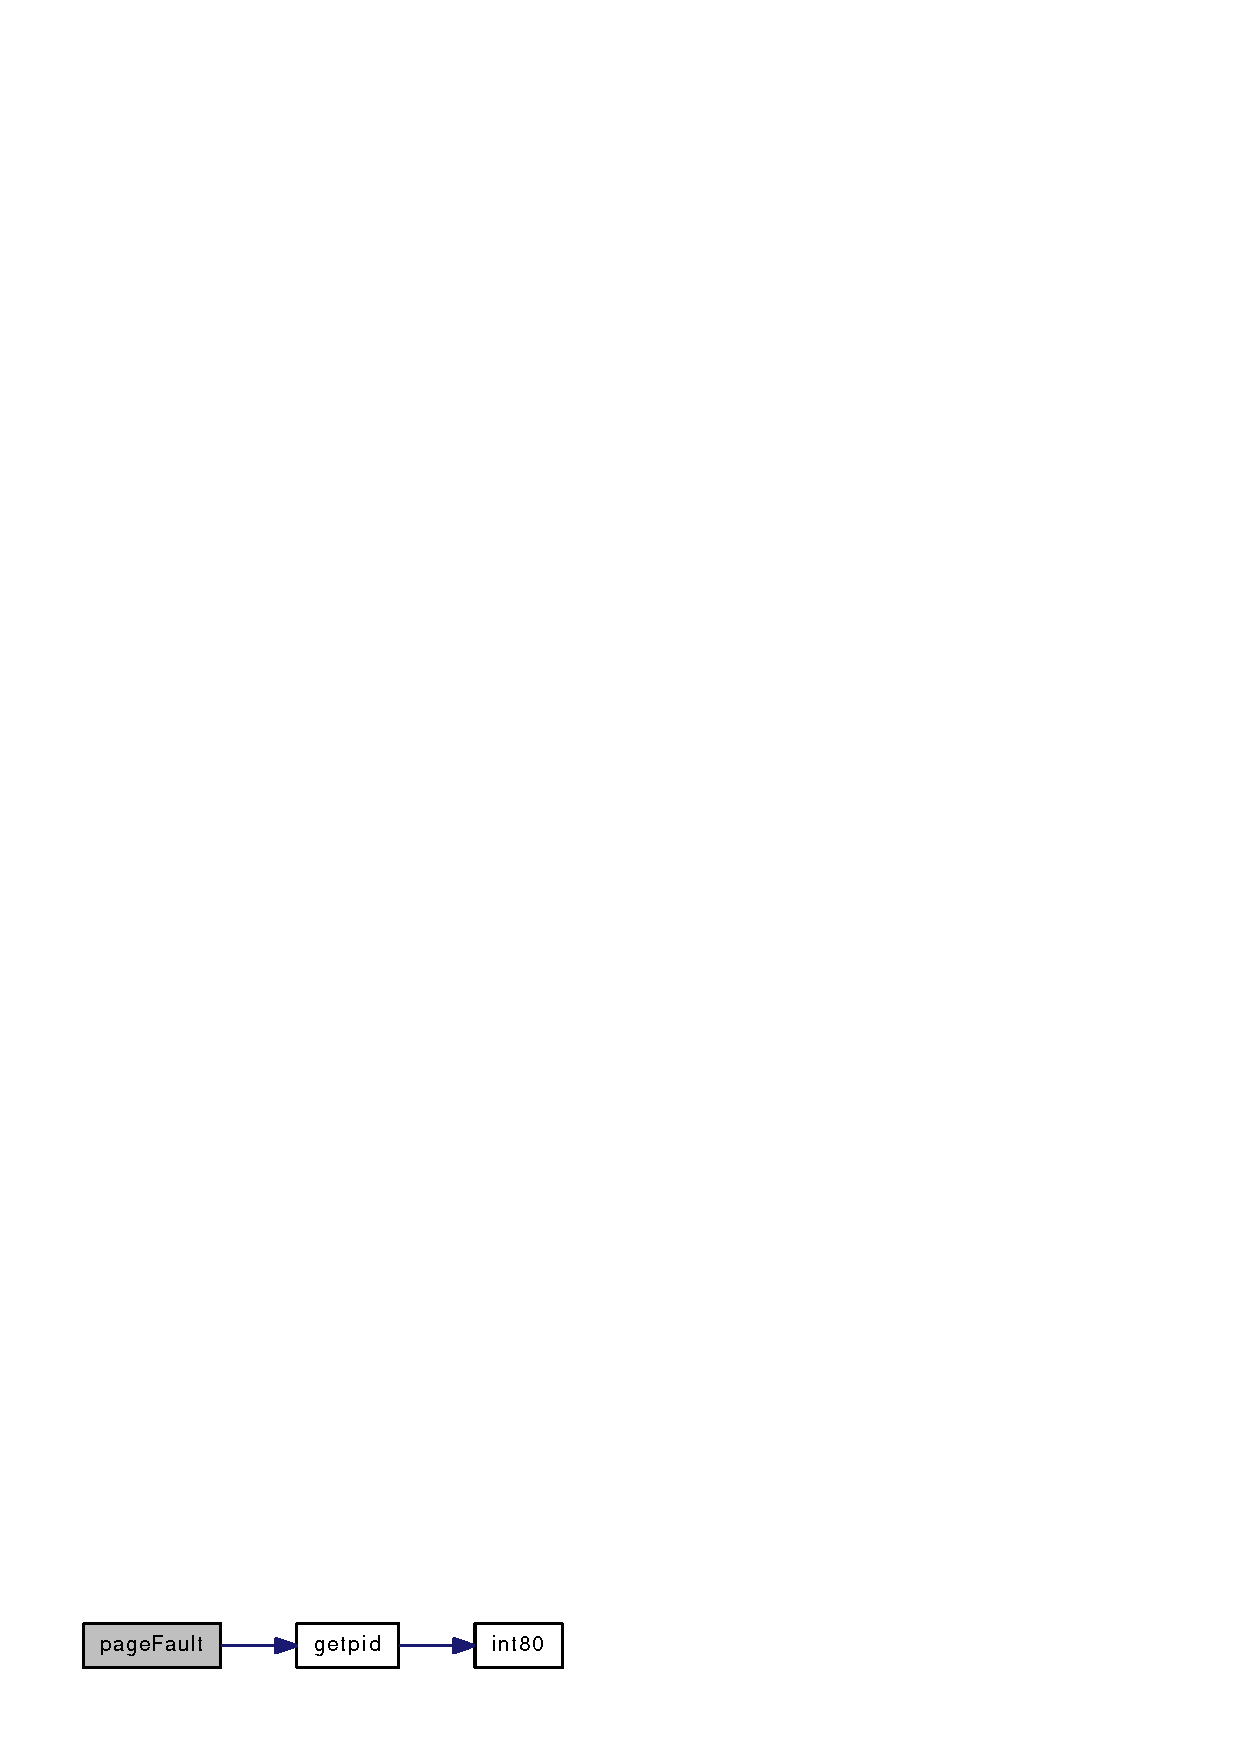
\includegraphics[width=137pt]{bin_8h_ab8d39c86e0f803f0816e787e36c99bd1_cgraph}
\end{center}
\end{figure}


\hypertarget{bin_8h_a8d6f8ce896cba69a844650449479ead1}{
\index{bin.h@{bin.h}!printA@{printA}}
\index{printA@{printA}!bin.h@{bin.h}}
\subsubsection[{printA}]{\setlength{\rightskip}{0pt plus 5cm}void printA ()}}
\label{bin_8h_a8d6f8ce896cba69a844650449479ead1}


This function prints infinite A letters. 

Use: 
\begin{DoxyCode}
                        createProcess("printA", (void(*)(void *))printA, NULL, 
      FOREGROUND)
\end{DoxyCode}


\begin{DoxySeeAlso}{See also}

\end{DoxySeeAlso}


Definition at line 291 of file bin.c.

\hypertarget{bin_8h_a5964c5b2b75cb7dc3c7648afe535fd03}{
\index{bin.h@{bin.h}!printB@{printB}}
\index{printB@{printB}!bin.h@{bin.h}}
\subsubsection[{printB}]{\setlength{\rightskip}{0pt plus 5cm}void printB ()}}
\label{bin_8h_a5964c5b2b75cb7dc3c7648afe535fd03}


This functions prints infinite A letters. 

Use: 
\begin{DoxyCode}
                        createProcess("printB", (void(*)(void *))printB, NULL, 
      FOREGROUND)
\end{DoxyCode}


\begin{DoxySeeAlso}{See also}

\end{DoxySeeAlso}


Definition at line 300 of file bin.c.

\hypertarget{bin_8h_a9795fbee9531f56aeda1376bf9934506}{
\index{bin.h@{bin.h}!top@{top}}
\index{top@{top}!bin.h@{bin.h}}
\subsubsection[{top}]{\setlength{\rightskip}{0pt plus 5cm}void top (char $\ast$ {\em args})}}
\label{bin_8h_a9795fbee9531f56aeda1376bf9934506}


This function show what percentage of the microprocessor it is using each process. When you write the command top in the shell, the process top will be created. 


\begin{DoxyParams}{Parameters}
\item[{\em args}]Use: 
\begin{DoxyCode}
                        createProcess("top", (void(*)(void *))top, NULL, 
      FOREGROUND);
\end{DoxyCode}
 \end{DoxyParams}


Definition at line 63 of file bin.c.



Here is the call graph for this function:\nopagebreak
\begin{figure}[H]
\begin{center}
\leavevmode
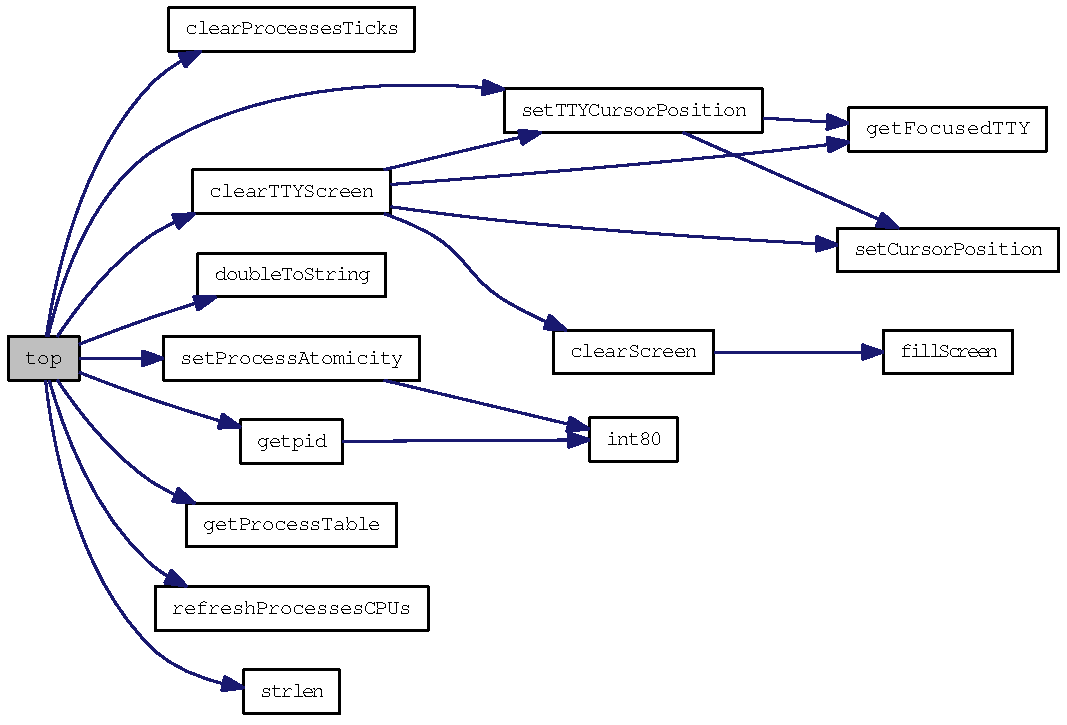
\includegraphics[width=274pt]{bin_8h_a9795fbee9531f56aeda1376bf9934506_cgraph}
\end{center}
\end{figure}


\hypertarget{bin_8h_a236e454e493fc9b262f746305660a2eb}{
\index{bin.h@{bin.h}!welcome@{welcome}}
\index{welcome@{welcome}!bin.h@{bin.h}}
\subsubsection[{welcome}]{\setlength{\rightskip}{0pt plus 5cm}void welcome ()}}
\label{bin_8h_a236e454e493fc9b262f746305660a2eb}


This function just prints the welcome message to Flying-\/High OS. 

Use: 
\begin{DoxyCode}
                        createProcess("welcome", (void(*)(void *))welcome, NULL, 
      FOREGROUND)
\end{DoxyCode}


\begin{DoxySeeAlso}{See also}

\end{DoxySeeAlso}


Definition at line 217 of file bin.c.



Here is the call graph for this function:\nopagebreak
\begin{figure}[H]
\begin{center}
\leavevmode
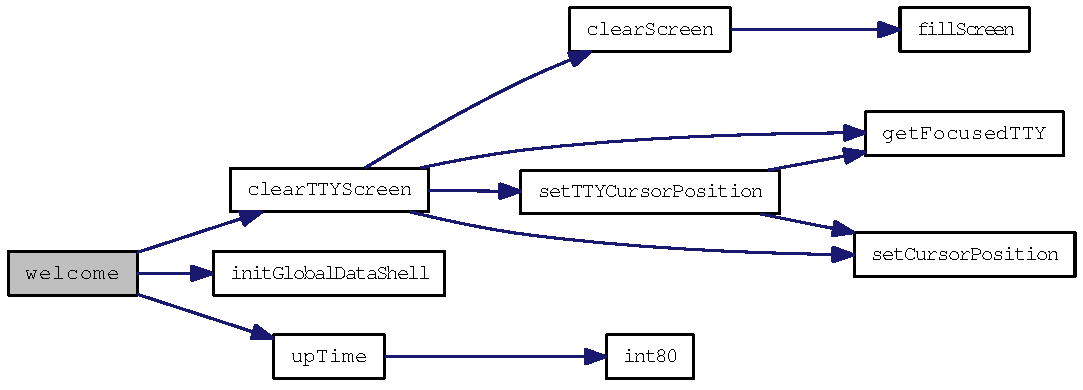
\includegraphics[width=278pt]{bin_8h_a236e454e493fc9b262f746305660a2eb_cgraph}
\end{center}
\end{figure}




Here is the caller graph for this function:\nopagebreak
\begin{figure}[H]
\begin{center}
\leavevmode
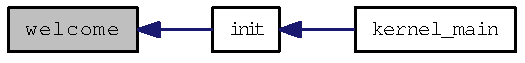
\includegraphics[width=144pt]{bin_8h_a236e454e493fc9b262f746305660a2eb_icgraph}
\end{center}
\end{figure}



\hypertarget{bttlship_8h}{
\section{inc/bttlship.h File Reference}
\label{bttlship_8h}\index{inc/bttlship.h@{inc/bttlship.h}}
}


The header file of the battleship game.  


{\ttfamily \#include \char`\"{}video\_\-driver.h\char`\"{}}\par
{\ttfamily \#include \char`\"{}stdio.h\char`\"{}}\par
{\ttfamily \#include \char`\"{}string.h\char`\"{}}\par
{\ttfamily \#include \char`\"{}types.h\char`\"{}}\par
{\ttfamily \#include \char`\"{}process.h\char`\"{}}\par
{\ttfamily \#include \char`\"{}shMemory.h\char`\"{}}\par
{\ttfamily \#include \char`\"{}semaphore.h\char`\"{}}\par
{\ttfamily \#include \char`\"{}rand.h\char`\"{}}\par
{\ttfamily \#include \char`\"{}ttys.h\char`\"{}}\par
Include dependency graph for bttlship.h:\nopagebreak
\begin{figure}[H]
\begin{center}
\leavevmode
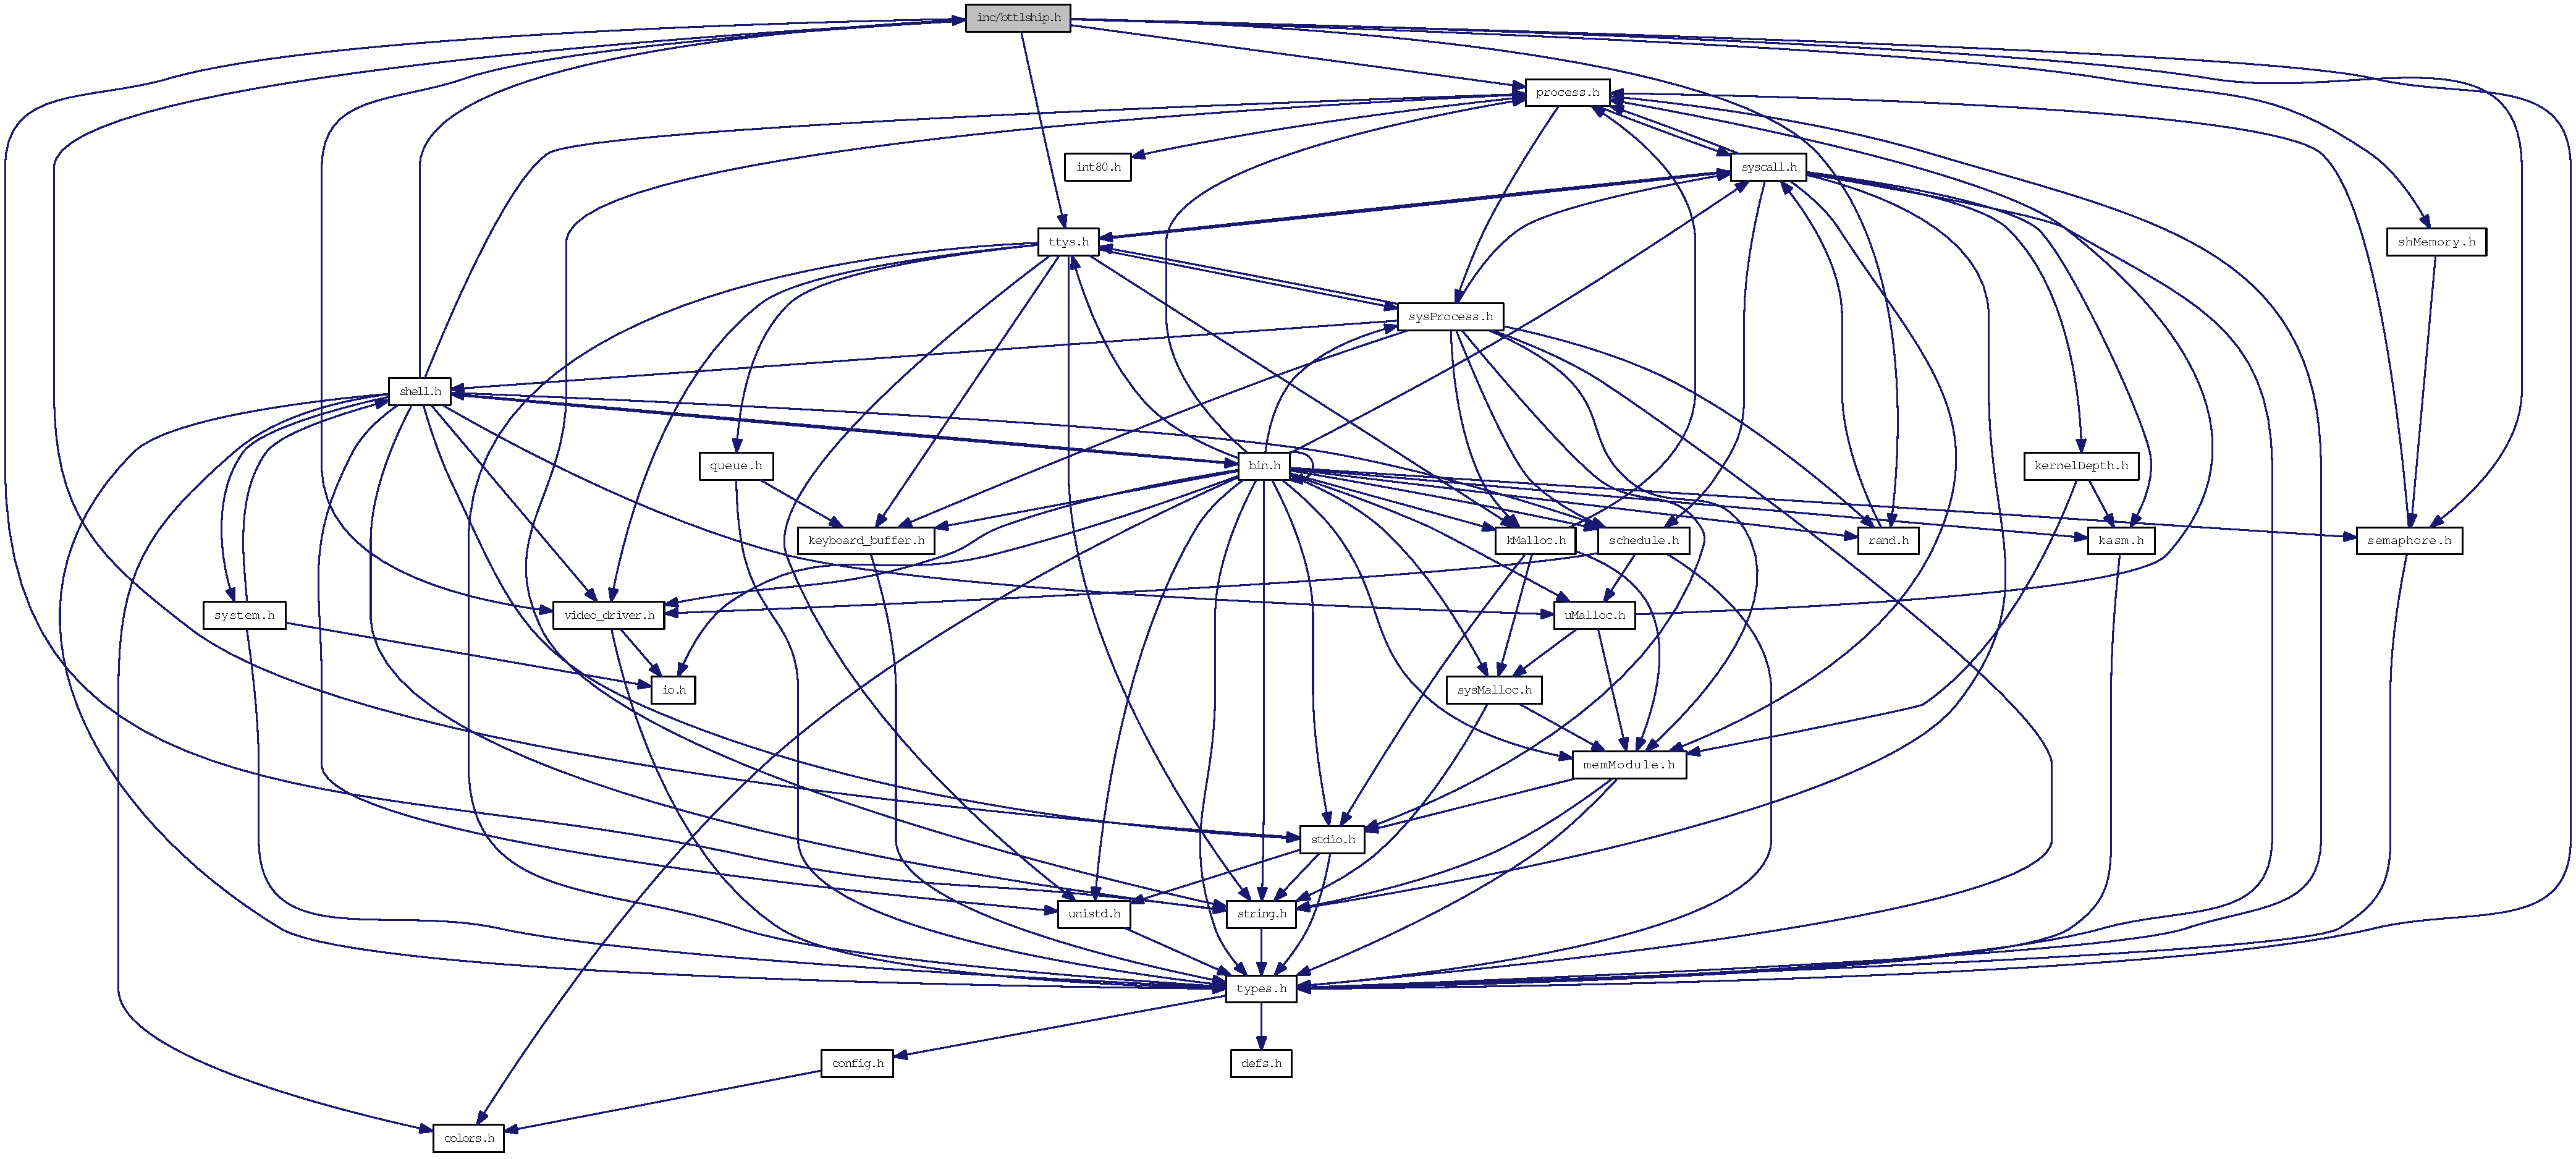
\includegraphics[width=420pt]{bttlship_8h__incl}
\end{center}
\end{figure}
This graph shows which files directly or indirectly include this file:\nopagebreak
\begin{figure}[H]
\begin{center}
\leavevmode
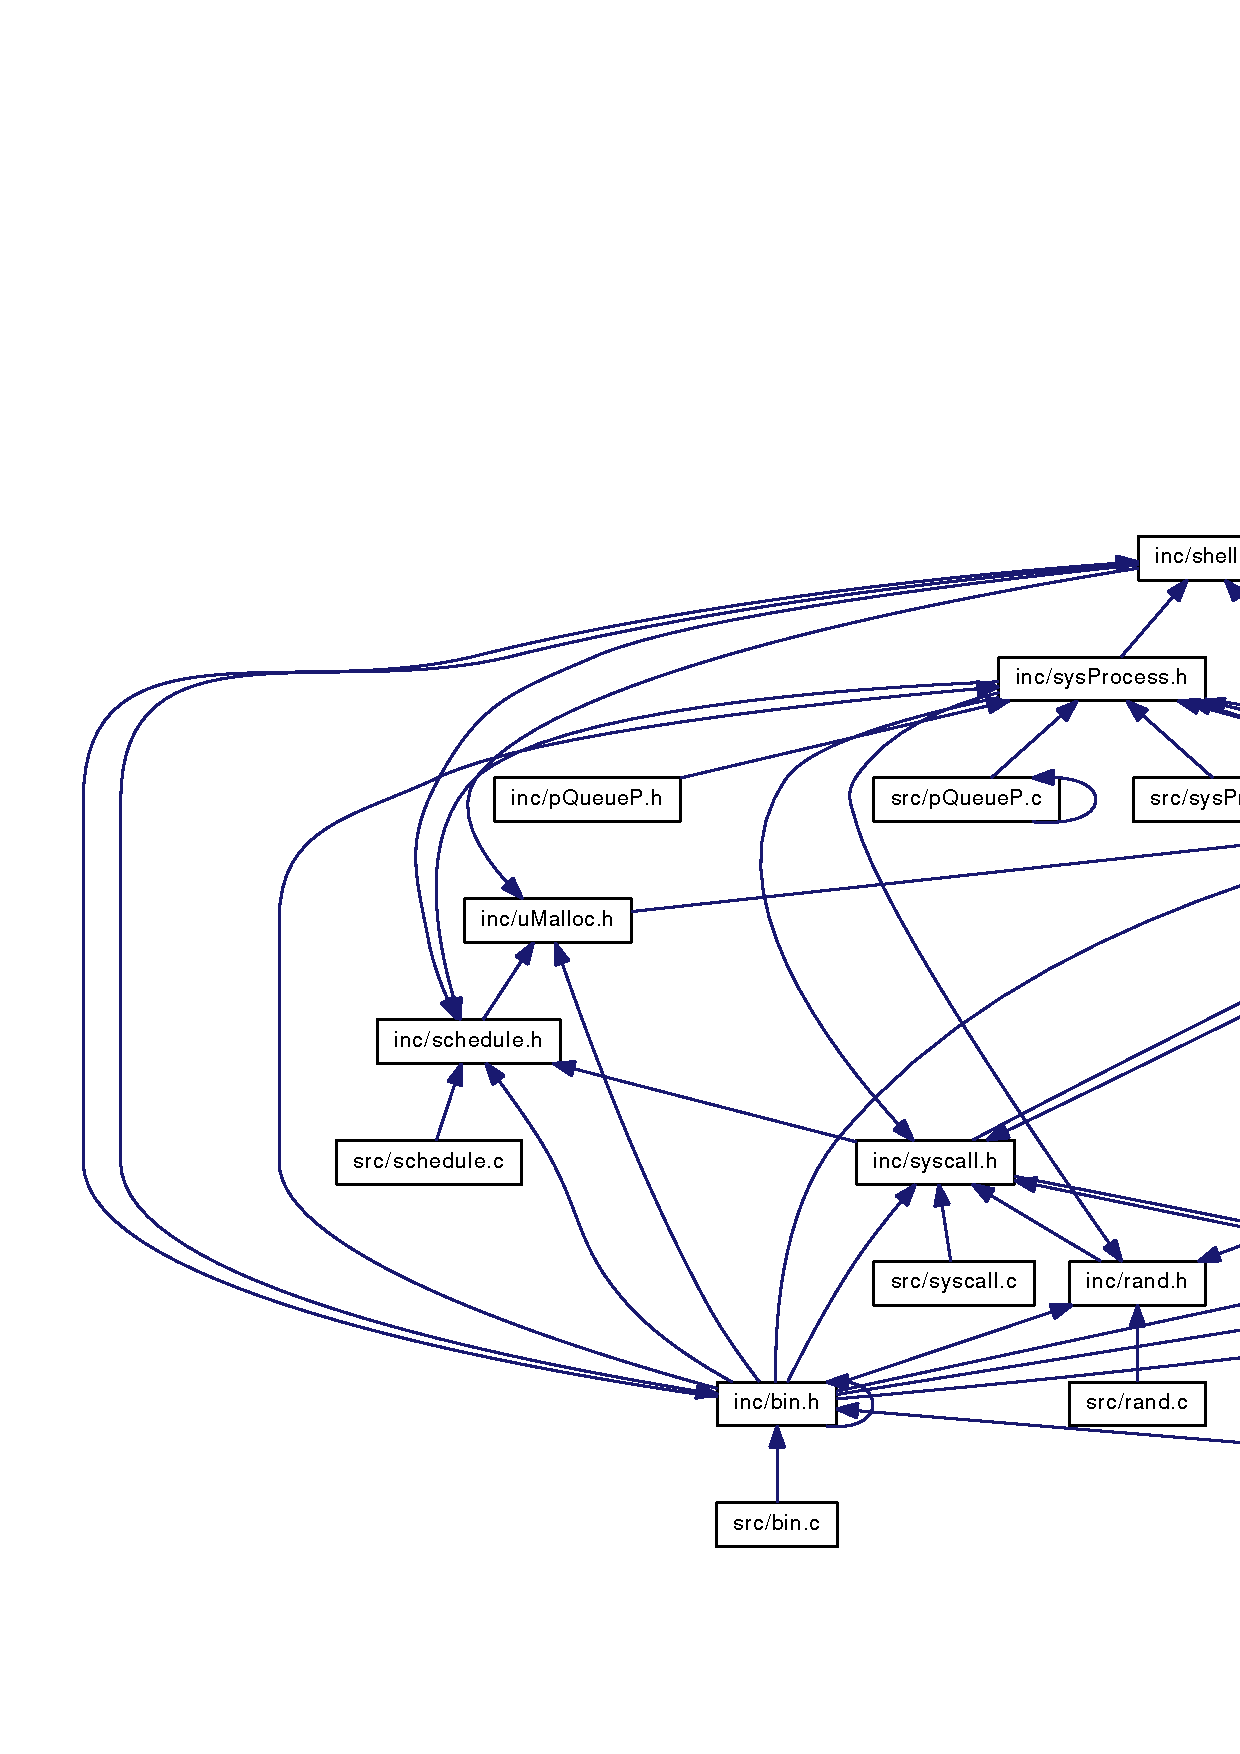
\includegraphics[width=420pt]{bttlship_8h__dep__incl}
\end{center}
\end{figure}
\subsection*{Data Structures}
\begin{DoxyCompactItemize}
\item 
struct \hyperlink{struct_s___t_a_b_l_e}{S\_\-TABLE}
\end{DoxyCompactItemize}
\subsection*{Defines}
\begin{DoxyCompactItemize}
\item 
\#define \hyperlink{bttlship_8h_a162b2f8daef7ed7ffb5b65eb52f06541}{N\_\-X}~10
\item 
\#define \hyperlink{bttlship_8h_a5efedafe88e8b42370ab7e629360d5b8}{N\_\-Y}~10
\item 
\#define \hyperlink{bttlship_8h_a4f5341d5491f9ca1655a283043276052}{N\_\-Z}~5
\item 
\#define \hyperlink{bttlship_8h_a1f3139d214f19c27732d952f9f47cdb7}{N\_\-SHIPS}~6
\item 
\#define \hyperlink{bttlship_8h_adacc98cbe6c9c29d073ce4e4e47d786c}{INP\_\-NONE}~0
\item 
\#define \hyperlink{bttlship_8h_a9975cd7a48b7b233f3785f04190f97eb}{INP\_\-YX}~1
\item 
\#define \hyperlink{bttlship_8h_a0376b2ead2de10bb7ab6a4d21ec304e9}{LOCK}~lockTable(0,1, \&table)
\item 
\#define \hyperlink{bttlship_8h_ac82effb31e82e32254efc8b57251d59e}{UNLOCK}~lockTable(0,0, \&table)
\item 
\#define \hyperlink{bttlship_8h_aa5c996b0f78c43badb720d4e71b36c47}{WAIT2}~lockTable(1,1, \&table)
\item 
\#define \hyperlink{bttlship_8h_a6d6f3072344ba56155dd8f035da07137}{NOTIFY2}~lockTable(1,0, \&table)
\item 
\#define \hyperlink{bttlship_8h_aa6b116f87a85ae940c89cdfc6f2581a7}{FLG\_\-P1}~001
\item 
\#define \hyperlink{bttlship_8h_a47bfd9d0735388bcd45193b3579ebd0f}{FLG\_\-P2}~002
\item 
\#define \hyperlink{bttlship_8h_a1cb9b8638cef6ff70f3b6178c07b6d79}{FLG\_\-SEEN0}~004
\item 
\#define \hyperlink{bttlship_8h_ae89a10b18e78db31e348765563a25d39}{FLG\_\-SEEN1}~010
\item 
\#define \hyperlink{bttlship_8h_a2459bbe0a47167492255693121680db5}{FLG\_\-BOMBD}~020
\item 
\#define \hyperlink{bttlship_8h_a5f70824b678311b0789ff323b32a2440}{FLG\_\-SPLSH}~040
\end{DoxyCompactItemize}
\subsection*{Typedefs}
\begin{DoxyCompactItemize}
\item 
typedef struct \hyperlink{struct_s___t_a_b_l_e}{S\_\-TABLE} \hyperlink{bttlship_8h_ae13bc024f7a68af424d382c4b7a9ce39}{S\_\-TABLE}
\end{DoxyCompactItemize}
\subsection*{Functions}
\begin{DoxyCompactItemize}
\item 
void \hyperlink{bttlship_8h_ac475b6f9eb4174c8579f3d4709b0e219}{cleanup} (\hyperlink{types_8h_a158b5efbc244b8995c439d60c976c818}{key\_\-t} shmid, \hyperlink{types_8h_a158b5efbc244b8995c439d60c976c818}{key\_\-t} semid)
\begin{DoxyCompactList}\small\item\em Destroys the used shared memory and semaphores. \item\end{DoxyCompactList}\item 
void \hyperlink{bttlship_8h_a03d7f39ab8509bab171aecf4d4fc7b9e}{attachTable} (\hyperlink{struct_s___t_a_b_l_e}{S\_\-TABLE} $\ast$$\ast$table, \hyperlink{types_8h_a158b5efbc244b8995c439d60c976c818}{key\_\-t} shmid, char $\ast$$\ast$shmp)
\begin{DoxyCompactList}\small\item\em It attaches itself to the already created memory. \item\end{DoxyCompactList}\item 
void \hyperlink{bttlship_8h_af66d7960a49eb99b5260ba4d524e1ac8}{lockTable} (int semx, int block, \hyperlink{struct_s___t_a_b_l_e}{S\_\-TABLE} $\ast$$\ast$tableS)
\begin{DoxyCompactList}\small\item\em It decides if it has to lock the table or wait for the opponent. Peform semaphore wait/notifies: ARGUMENTS: semx 0 : table lock semaphore 1 : opponent notify semaphore block 0 : perform notify 1 : perform wait. \item\end{DoxyCompactList}\item 
void \hyperlink{bttlship_8h_a03efcb954008fc3018e19f0353b58157}{recount} (\hyperlink{struct_s___t_a_b_l_e}{S\_\-TABLE} $\ast$$\ast$tableS, int $\ast$flg\_\-game\_\-over)
\begin{DoxyCompactList}\small\item\em It counts the amount of bombs that the player has left. \item\end{DoxyCompactList}\item 
void \hyperlink{bttlship_8h_aef4b6e9d64c7bff5215251a7bec36b37}{bomb} (int x, int y, \hyperlink{struct_s___t_a_b_l_e}{S\_\-TABLE} $\ast$$\ast$tableS)
\begin{DoxyCompactList}\small\item\em It puts the bomb on a specific position of the table. \item\end{DoxyCompactList}\item 
int \hyperlink{bttlship_8h_a4003a14058da5be60c7e7600713cd5c0}{getInput} (int $\ast$px, int $\ast$py, \hyperlink{struct_s___t_a_b_l_e}{S\_\-TABLE} $\ast$$\ast$table)
\begin{DoxyCompactList}\small\item\em It obtains the the row and the column of the table from STDIN. \item\end{DoxyCompactList}\item 
int \hyperlink{bttlship_8h_a6554029a39cab2edd50f67075f949926}{draw\_\-hz} (int sx, int sy, int z, int who, \hyperlink{struct_s___t_a_b_l_e}{S\_\-TABLE} $\ast$$\ast$tableS)
\begin{DoxyCompactList}\small\item\em It draws the horizontal ship. \item\end{DoxyCompactList}\item 
int \hyperlink{bttlship_8h_a2d3705cb0dd809d88cd03e1bb39afb09}{draw\_\-vt} (int sx, int sy, int z, int who, \hyperlink{struct_s___t_a_b_l_e}{S\_\-TABLE} $\ast$$\ast$tableS)
\begin{DoxyCompactList}\small\item\em It draws the horizontal ship. \item\end{DoxyCompactList}\item 
void \hyperlink{bttlship_8h_ae442293b5a53448d5a03e47e38396009}{genBattle} (\hyperlink{struct_s___t_a_b_l_e}{S\_\-TABLE} $\ast$$\ast$tableS)
\begin{DoxyCompactList}\small\item\em It generates the table. \item\end{DoxyCompactList}\item 
void \hyperlink{bttlship_8h_afcb21d332942ec61fd523fed20b758e5}{showRow} (void)
\begin{DoxyCompactList}\small\item\em It prints each row of the table. \item\end{DoxyCompactList}\item 
void \hyperlink{bttlship_8h_a21c4f719d9c70f144ffbb7b4ab57d935}{showBattle} (\hyperlink{struct_s___t_a_b_l_e}{S\_\-TABLE} $\ast$$\ast$tableS, int us, int them, int $\ast$flg\_\-game\_\-over)
\begin{DoxyCompactList}\small\item\em It prints the table of the battlehsip. \item\end{DoxyCompactList}\item 
int \hyperlink{bttlship_8h_a52e47768a66b91e89d5546a8cb0f168c}{battleship} ()
\begin{DoxyCompactList}\small\item\em It's the main process of the battleship, it generates the whole table and ships. \item\end{DoxyCompactList}\end{DoxyCompactItemize}


\subsection{Detailed Description}
The header file of the battleship game. \begin{DoxyAuthor}{Author}
Luciano Zemin, Nicolás Magni, Nicolás Purita 
\end{DoxyAuthor}


Definition in file \hyperlink{bttlship_8h_source}{bttlship.h}.



\subsection{Define Documentation}
\hypertarget{bttlship_8h_a2459bbe0a47167492255693121680db5}{
\index{bttlship.h@{bttlship.h}!FLG\_\-BOMBD@{FLG\_\-BOMBD}}
\index{FLG\_\-BOMBD@{FLG\_\-BOMBD}!bttlship.h@{bttlship.h}}
\subsubsection[{FLG\_\-BOMBD}]{\setlength{\rightskip}{0pt plus 5cm}\#define FLG\_\-BOMBD~020}}
\label{bttlship_8h_a2459bbe0a47167492255693121680db5}


Definition at line 44 of file bttlship.h.

\hypertarget{bttlship_8h_aa6b116f87a85ae940c89cdfc6f2581a7}{
\index{bttlship.h@{bttlship.h}!FLG\_\-P1@{FLG\_\-P1}}
\index{FLG\_\-P1@{FLG\_\-P1}!bttlship.h@{bttlship.h}}
\subsubsection[{FLG\_\-P1}]{\setlength{\rightskip}{0pt plus 5cm}\#define FLG\_\-P1~001}}
\label{bttlship_8h_aa6b116f87a85ae940c89cdfc6f2581a7}


Definition at line 40 of file bttlship.h.

\hypertarget{bttlship_8h_a47bfd9d0735388bcd45193b3579ebd0f}{
\index{bttlship.h@{bttlship.h}!FLG\_\-P2@{FLG\_\-P2}}
\index{FLG\_\-P2@{FLG\_\-P2}!bttlship.h@{bttlship.h}}
\subsubsection[{FLG\_\-P2}]{\setlength{\rightskip}{0pt plus 5cm}\#define FLG\_\-P2~002}}
\label{bttlship_8h_a47bfd9d0735388bcd45193b3579ebd0f}


Definition at line 41 of file bttlship.h.

\hypertarget{bttlship_8h_a1cb9b8638cef6ff70f3b6178c07b6d79}{
\index{bttlship.h@{bttlship.h}!FLG\_\-SEEN0@{FLG\_\-SEEN0}}
\index{FLG\_\-SEEN0@{FLG\_\-SEEN0}!bttlship.h@{bttlship.h}}
\subsubsection[{FLG\_\-SEEN0}]{\setlength{\rightskip}{0pt plus 5cm}\#define FLG\_\-SEEN0~004}}
\label{bttlship_8h_a1cb9b8638cef6ff70f3b6178c07b6d79}


Definition at line 42 of file bttlship.h.

\hypertarget{bttlship_8h_ae89a10b18e78db31e348765563a25d39}{
\index{bttlship.h@{bttlship.h}!FLG\_\-SEEN1@{FLG\_\-SEEN1}}
\index{FLG\_\-SEEN1@{FLG\_\-SEEN1}!bttlship.h@{bttlship.h}}
\subsubsection[{FLG\_\-SEEN1}]{\setlength{\rightskip}{0pt plus 5cm}\#define FLG\_\-SEEN1~010}}
\label{bttlship_8h_ae89a10b18e78db31e348765563a25d39}


Definition at line 43 of file bttlship.h.

\hypertarget{bttlship_8h_a5f70824b678311b0789ff323b32a2440}{
\index{bttlship.h@{bttlship.h}!FLG\_\-SPLSH@{FLG\_\-SPLSH}}
\index{FLG\_\-SPLSH@{FLG\_\-SPLSH}!bttlship.h@{bttlship.h}}
\subsubsection[{FLG\_\-SPLSH}]{\setlength{\rightskip}{0pt plus 5cm}\#define FLG\_\-SPLSH~040}}
\label{bttlship_8h_a5f70824b678311b0789ff323b32a2440}


Definition at line 45 of file bttlship.h.

\hypertarget{bttlship_8h_adacc98cbe6c9c29d073ce4e4e47d786c}{
\index{bttlship.h@{bttlship.h}!INP\_\-NONE@{INP\_\-NONE}}
\index{INP\_\-NONE@{INP\_\-NONE}!bttlship.h@{bttlship.h}}
\subsubsection[{INP\_\-NONE}]{\setlength{\rightskip}{0pt plus 5cm}\#define INP\_\-NONE~0}}
\label{bttlship_8h_adacc98cbe6c9c29d073ce4e4e47d786c}


Definition at line 28 of file bttlship.h.

\hypertarget{bttlship_8h_a9975cd7a48b7b233f3785f04190f97eb}{
\index{bttlship.h@{bttlship.h}!INP\_\-YX@{INP\_\-YX}}
\index{INP\_\-YX@{INP\_\-YX}!bttlship.h@{bttlship.h}}
\subsubsection[{INP\_\-YX}]{\setlength{\rightskip}{0pt plus 5cm}\#define INP\_\-YX~1}}
\label{bttlship_8h_a9975cd7a48b7b233f3785f04190f97eb}


Definition at line 29 of file bttlship.h.

\hypertarget{bttlship_8h_a0376b2ead2de10bb7ab6a4d21ec304e9}{
\index{bttlship.h@{bttlship.h}!LOCK@{LOCK}}
\index{LOCK@{LOCK}!bttlship.h@{bttlship.h}}
\subsubsection[{LOCK}]{\setlength{\rightskip}{0pt plus 5cm}\#define LOCK~lockTable(0,1, \&table)}}
\label{bttlship_8h_a0376b2ead2de10bb7ab6a4d21ec304e9}


Definition at line 31 of file bttlship.h.

\hypertarget{bttlship_8h_a1f3139d214f19c27732d952f9f47cdb7}{
\index{bttlship.h@{bttlship.h}!N\_\-SHIPS@{N\_\-SHIPS}}
\index{N\_\-SHIPS@{N\_\-SHIPS}!bttlship.h@{bttlship.h}}
\subsubsection[{N\_\-SHIPS}]{\setlength{\rightskip}{0pt plus 5cm}\#define N\_\-SHIPS~6}}
\label{bttlship_8h_a1f3139d214f19c27732d952f9f47cdb7}


Definition at line 26 of file bttlship.h.

\hypertarget{bttlship_8h_a162b2f8daef7ed7ffb5b65eb52f06541}{
\index{bttlship.h@{bttlship.h}!N\_\-X@{N\_\-X}}
\index{N\_\-X@{N\_\-X}!bttlship.h@{bttlship.h}}
\subsubsection[{N\_\-X}]{\setlength{\rightskip}{0pt plus 5cm}\#define N\_\-X~10}}
\label{bttlship_8h_a162b2f8daef7ed7ffb5b65eb52f06541}


Definition at line 23 of file bttlship.h.

\hypertarget{bttlship_8h_a5efedafe88e8b42370ab7e629360d5b8}{
\index{bttlship.h@{bttlship.h}!N\_\-Y@{N\_\-Y}}
\index{N\_\-Y@{N\_\-Y}!bttlship.h@{bttlship.h}}
\subsubsection[{N\_\-Y}]{\setlength{\rightskip}{0pt plus 5cm}\#define N\_\-Y~10}}
\label{bttlship_8h_a5efedafe88e8b42370ab7e629360d5b8}


Definition at line 24 of file bttlship.h.

\hypertarget{bttlship_8h_a4f5341d5491f9ca1655a283043276052}{
\index{bttlship.h@{bttlship.h}!N\_\-Z@{N\_\-Z}}
\index{N\_\-Z@{N\_\-Z}!bttlship.h@{bttlship.h}}
\subsubsection[{N\_\-Z}]{\setlength{\rightskip}{0pt plus 5cm}\#define N\_\-Z~5}}
\label{bttlship_8h_a4f5341d5491f9ca1655a283043276052}


Definition at line 25 of file bttlship.h.

\hypertarget{bttlship_8h_a6d6f3072344ba56155dd8f035da07137}{
\index{bttlship.h@{bttlship.h}!NOTIFY2@{NOTIFY2}}
\index{NOTIFY2@{NOTIFY2}!bttlship.h@{bttlship.h}}
\subsubsection[{NOTIFY2}]{\setlength{\rightskip}{0pt plus 5cm}\#define NOTIFY2~lockTable(1,0, \&table)}}
\label{bttlship_8h_a6d6f3072344ba56155dd8f035da07137}


Definition at line 35 of file bttlship.h.

\hypertarget{bttlship_8h_ac82effb31e82e32254efc8b57251d59e}{
\index{bttlship.h@{bttlship.h}!UNLOCK@{UNLOCK}}
\index{UNLOCK@{UNLOCK}!bttlship.h@{bttlship.h}}
\subsubsection[{UNLOCK}]{\setlength{\rightskip}{0pt plus 5cm}\#define UNLOCK~lockTable(0,0, \&table)}}
\label{bttlship_8h_ac82effb31e82e32254efc8b57251d59e}


Definition at line 32 of file bttlship.h.

\hypertarget{bttlship_8h_aa5c996b0f78c43badb720d4e71b36c47}{
\index{bttlship.h@{bttlship.h}!WAIT2@{WAIT2}}
\index{WAIT2@{WAIT2}!bttlship.h@{bttlship.h}}
\subsubsection[{WAIT2}]{\setlength{\rightskip}{0pt plus 5cm}\#define WAIT2~lockTable(1,1, \&table)}}
\label{bttlship_8h_aa5c996b0f78c43badb720d4e71b36c47}


Definition at line 34 of file bttlship.h.



\subsection{Typedef Documentation}
\hypertarget{bttlship_8h_ae13bc024f7a68af424d382c4b7a9ce39}{
\index{bttlship.h@{bttlship.h}!S\_\-TABLE@{S\_\-TABLE}}
\index{S\_\-TABLE@{S\_\-TABLE}!bttlship.h@{bttlship.h}}
\subsubsection[{S\_\-TABLE}]{\setlength{\rightskip}{0pt plus 5cm}typedef struct {\bf S\_\-TABLE} {\bf S\_\-TABLE}}}
\label{bttlship_8h_ae13bc024f7a68af424d382c4b7a9ce39}


\subsection{Function Documentation}
\hypertarget{bttlship_8h_a03d7f39ab8509bab171aecf4d4fc7b9e}{
\index{bttlship.h@{bttlship.h}!attachTable@{attachTable}}
\index{attachTable@{attachTable}!bttlship.h@{bttlship.h}}
\subsubsection[{attachTable}]{\setlength{\rightskip}{0pt plus 5cm}void attachTable ({\bf S\_\-TABLE} $\ast$$\ast$ {\em table}, \/  {\bf key\_\-t} {\em shmid}, \/  char $\ast$$\ast$ {\em shmp})}}
\label{bttlship_8h_a03d7f39ab8509bab171aecf4d4fc7b9e}


It attaches itself to the already created memory. 


\begin{DoxyParams}{Parameters}
\item[{\em table}]The adress of the table. \item[{\em shmid}]The shared memory segment id. \item[{\em shmp}]The adress where to store the shared memory segment pointer. \end{DoxyParams}


Definition at line 195 of file bttlship.c.



Here is the call graph for this function:\nopagebreak
\begin{figure}[H]
\begin{center}
\leavevmode
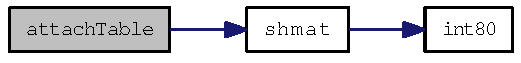
\includegraphics[width=143pt]{bttlship_8h_a03d7f39ab8509bab171aecf4d4fc7b9e_cgraph}
\end{center}
\end{figure}




Here is the caller graph for this function:\nopagebreak
\begin{figure}[H]
\begin{center}
\leavevmode
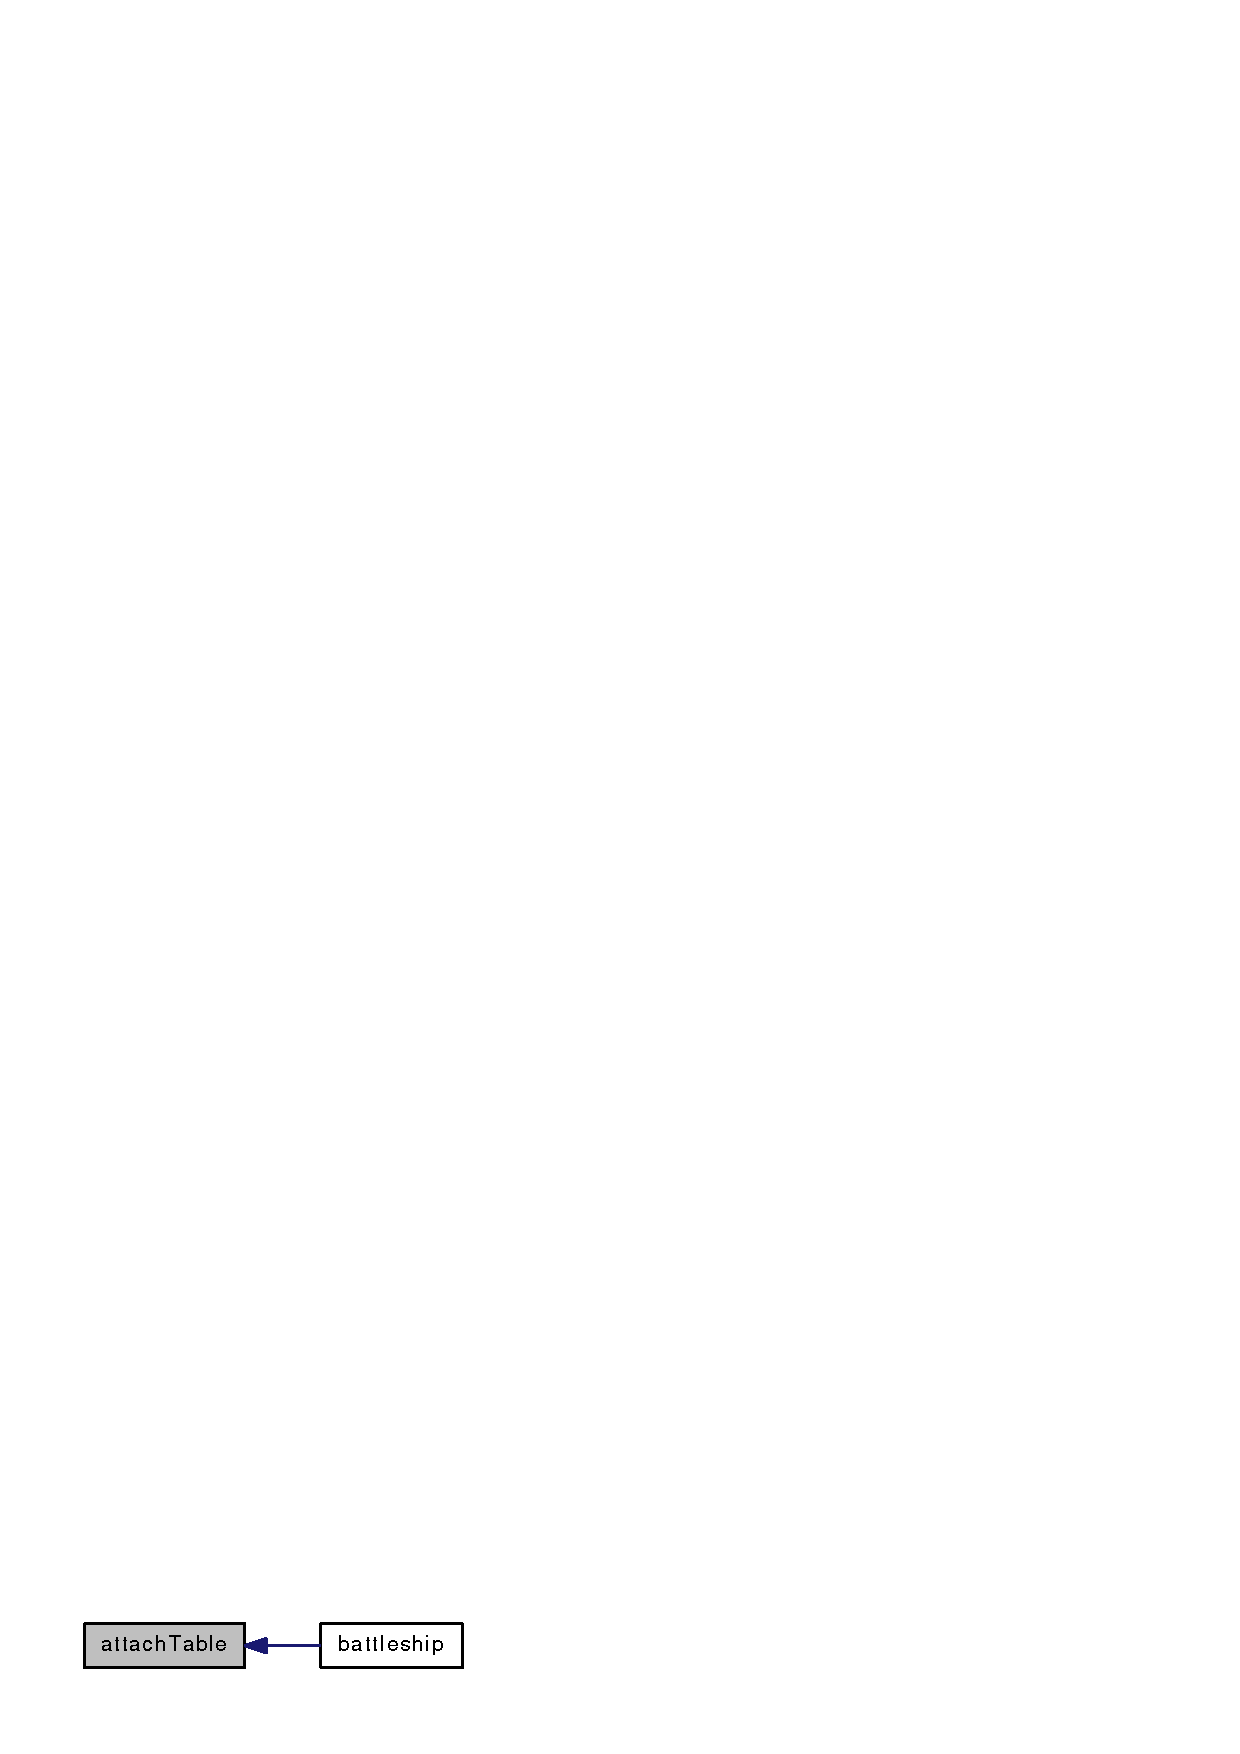
\includegraphics[width=113pt]{bttlship_8h_a03d7f39ab8509bab171aecf4d4fc7b9e_icgraph}
\end{center}
\end{figure}


\hypertarget{bttlship_8h_a52e47768a66b91e89d5546a8cb0f168c}{
\index{bttlship.h@{bttlship.h}!battleship@{battleship}}
\index{battleship@{battleship}!bttlship.h@{bttlship.h}}
\subsubsection[{battleship}]{\setlength{\rightskip}{0pt plus 5cm}int battleship ()}}
\label{bttlship_8h_a52e47768a66b91e89d5546a8cb0f168c}


It's the main process of the battleship, it generates the whole table and ships. 



Definition at line 12 of file bttlship.c.



Here is the call graph for this function:\nopagebreak
\begin{figure}[H]
\begin{center}
\leavevmode
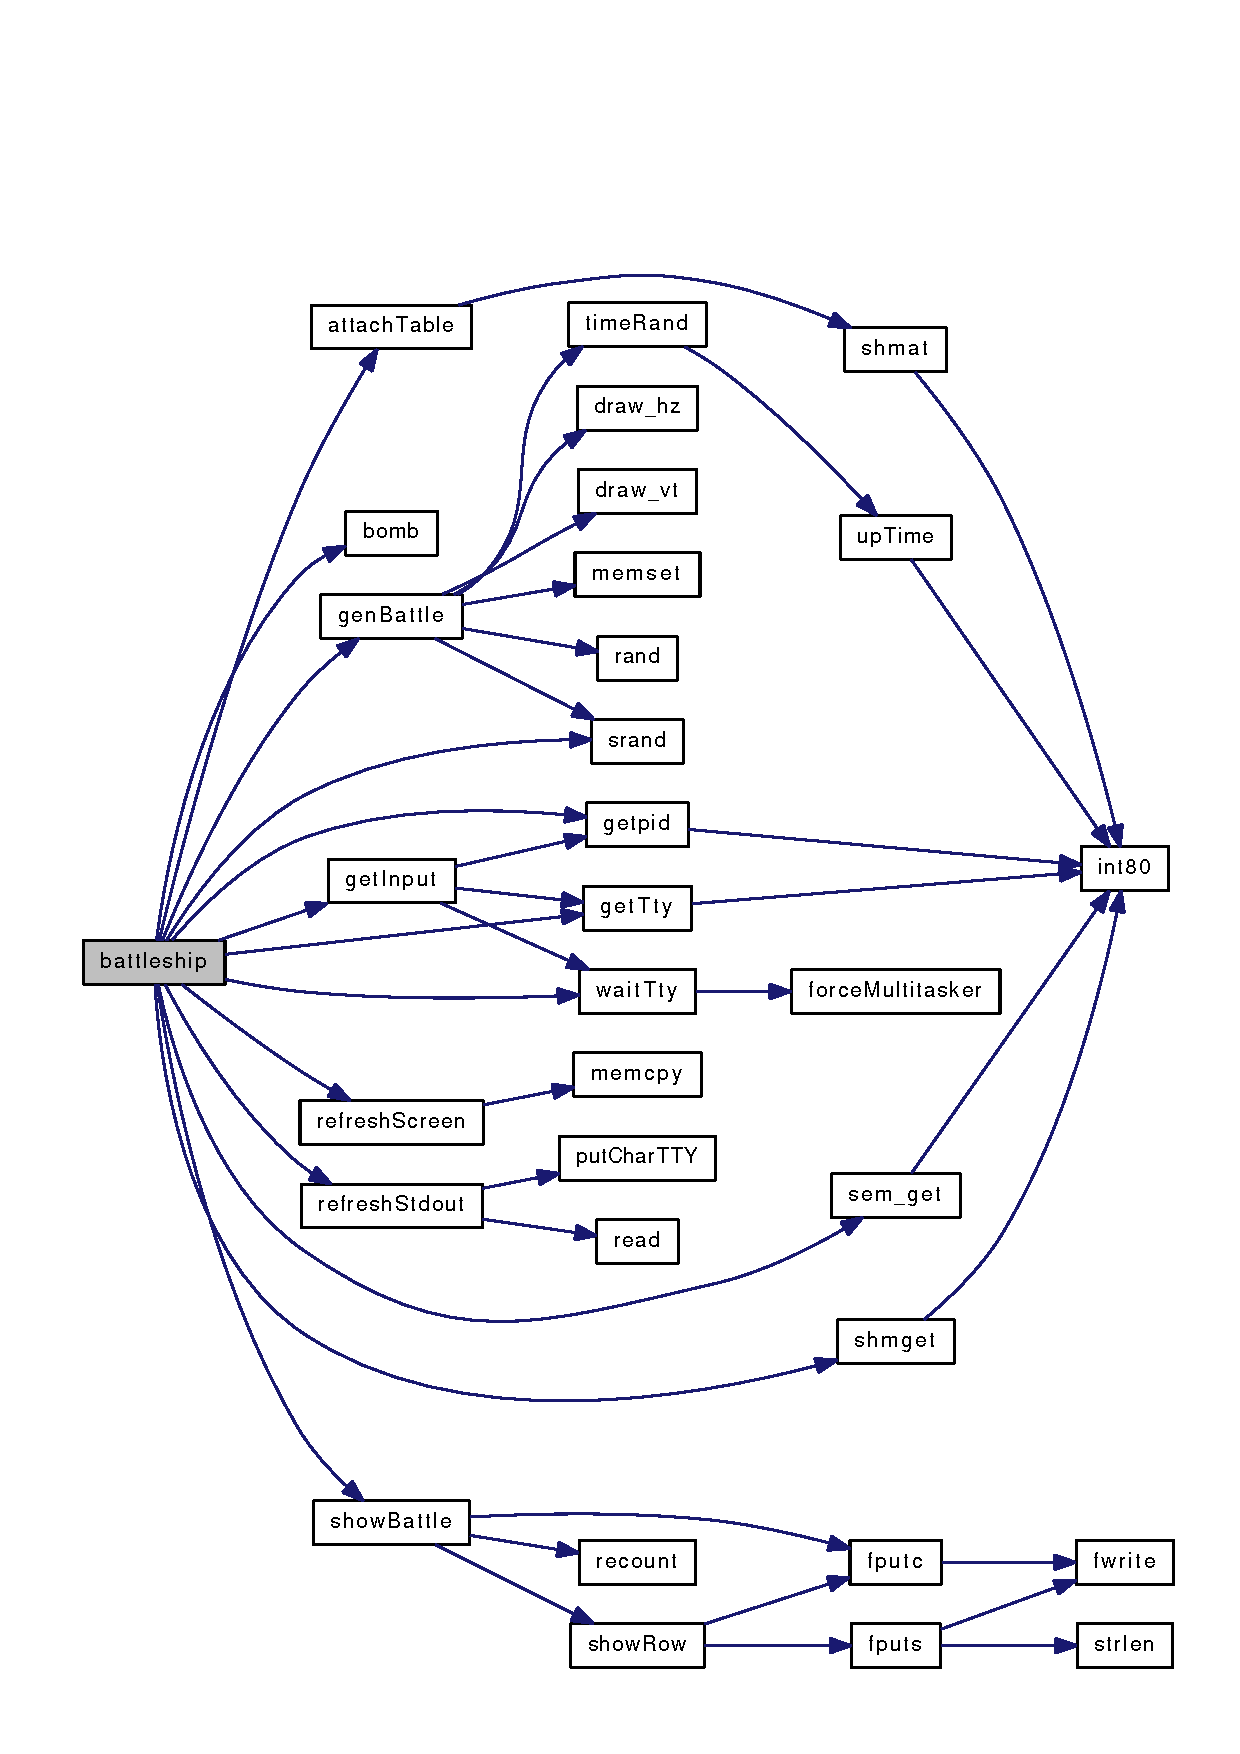
\includegraphics[width=284pt]{bttlship_8h_a52e47768a66b91e89d5546a8cb0f168c_cgraph}
\end{center}
\end{figure}


\hypertarget{bttlship_8h_aef4b6e9d64c7bff5215251a7bec36b37}{
\index{bttlship.h@{bttlship.h}!bomb@{bomb}}
\index{bomb@{bomb}!bttlship.h@{bttlship.h}}
\subsubsection[{bomb}]{\setlength{\rightskip}{0pt plus 5cm}void bomb (int {\em x}, \/  int {\em y}, \/  {\bf S\_\-TABLE} $\ast$$\ast$ {\em tableS})}}
\label{bttlship_8h_aef4b6e9d64c7bff5215251a7bec36b37}


It puts the bomb on a specific position of the table. 


\begin{DoxyParams}{Parameters}
\item[{\em x}]The row of the table \item[{\em y}]The column of the table \item[{\em tableS}]The address of the table. \end{DoxyParams}


Definition at line 231 of file bttlship.c.



Here is the caller graph for this function:\nopagebreak
\begin{figure}[H]
\begin{center}
\leavevmode
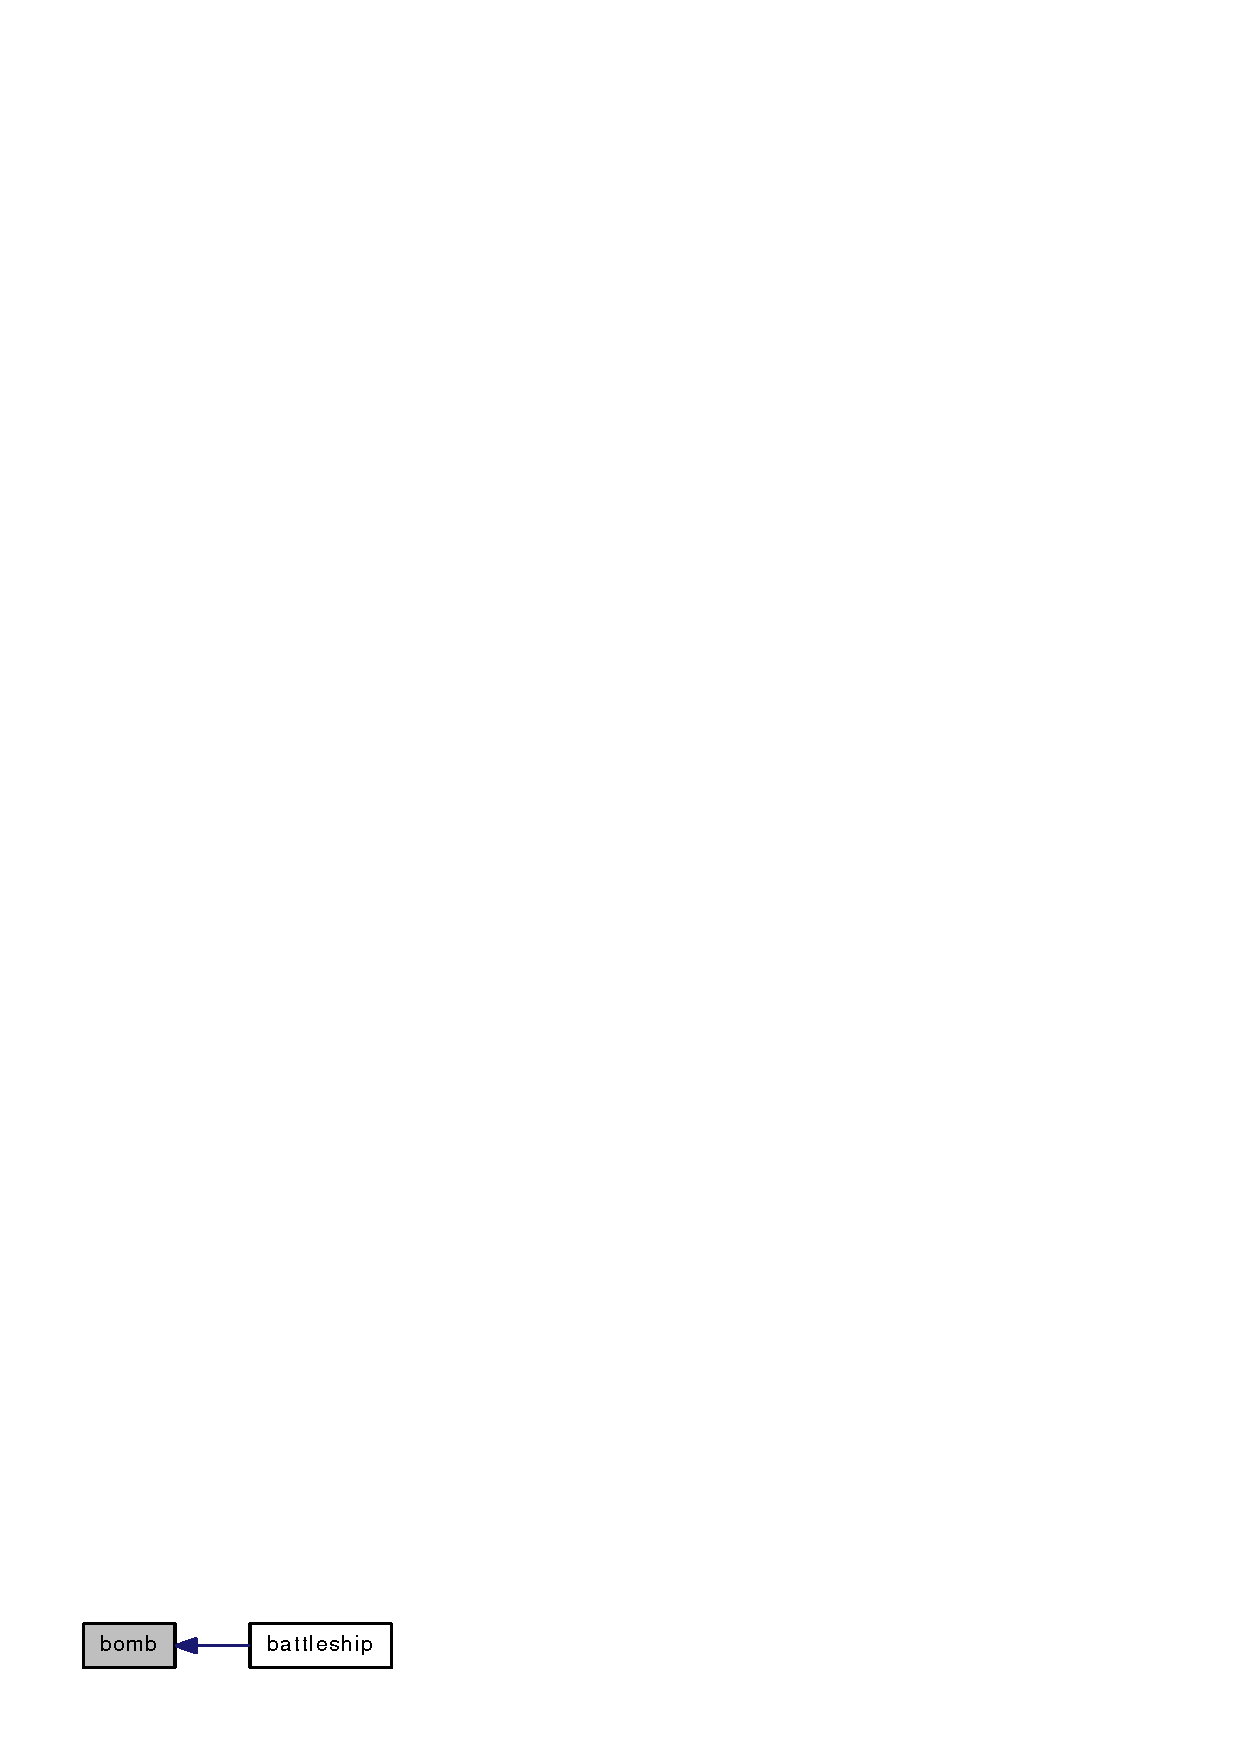
\includegraphics[width=96pt]{bttlship_8h_aef4b6e9d64c7bff5215251a7bec36b37_icgraph}
\end{center}
\end{figure}


\hypertarget{bttlship_8h_ac475b6f9eb4174c8579f3d4709b0e219}{
\index{bttlship.h@{bttlship.h}!cleanup@{cleanup}}
\index{cleanup@{cleanup}!bttlship.h@{bttlship.h}}
\subsubsection[{cleanup}]{\setlength{\rightskip}{0pt plus 5cm}void cleanup ({\bf key\_\-t} {\em shmid}, \/  {\bf key\_\-t} {\em semid})}}
\label{bttlship_8h_ac475b6f9eb4174c8579f3d4709b0e219}


Destroys the used shared memory and semaphores. 


\begin{DoxyParams}{Parameters}
\item[{\em shmid}]The id of the shared memory segment. \item[{\em semid}]The id of the semaphore. \end{DoxyParams}


Definition at line 186 of file bttlship.c.



Here is the call graph for this function:\nopagebreak
\begin{figure}[H]
\begin{center}
\leavevmode
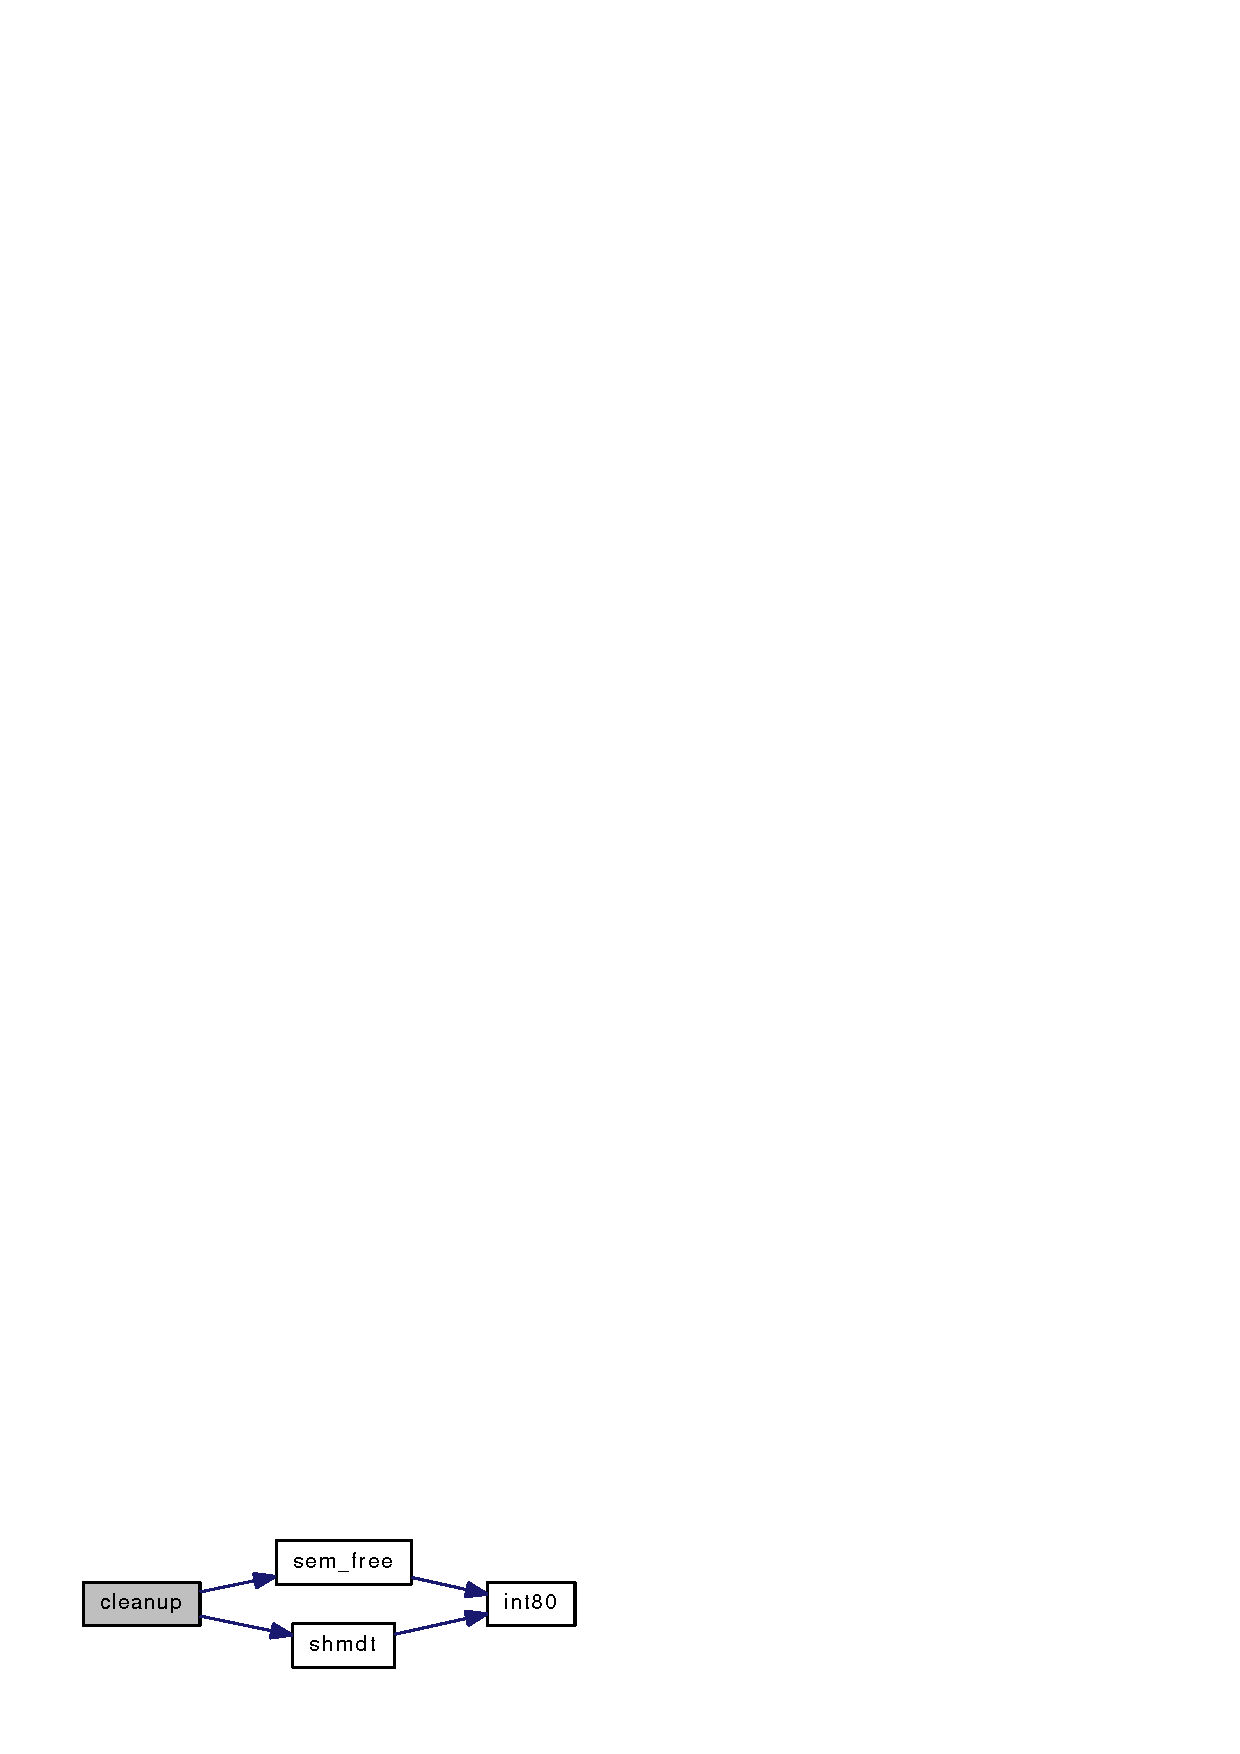
\includegraphics[width=140pt]{bttlship_8h_ac475b6f9eb4174c8579f3d4709b0e219_cgraph}
\end{center}
\end{figure}


\hypertarget{bttlship_8h_a6554029a39cab2edd50f67075f949926}{
\index{bttlship.h@{bttlship.h}!draw\_\-hz@{draw\_\-hz}}
\index{draw\_\-hz@{draw\_\-hz}!bttlship.h@{bttlship.h}}
\subsubsection[{draw\_\-hz}]{\setlength{\rightskip}{0pt plus 5cm}int draw\_\-hz (int {\em sx}, \/  int {\em sy}, \/  int {\em z}, \/  int {\em who}, \/  {\bf S\_\-TABLE} $\ast$$\ast$ {\em tableS})}}
\label{bttlship_8h_a6554029a39cab2edd50f67075f949926}


It draws the horizontal ship. 


\begin{DoxyParams}{Parameters}
\item[{\em sx}]Inner use. \item[{\em sy}]Inner use. \item[{\em z}]Inner use. \item[{\em who}]Iner use. \item[{\em tableS}]The address of the table. \end{DoxyParams}


Definition at line 283 of file bttlship.c.



Here is the caller graph for this function:\nopagebreak
\begin{figure}[H]
\begin{center}
\leavevmode
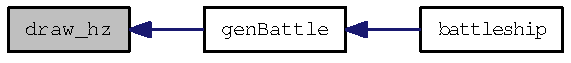
\includegraphics[width=155pt]{bttlship_8h_a6554029a39cab2edd50f67075f949926_icgraph}
\end{center}
\end{figure}


\hypertarget{bttlship_8h_a2d3705cb0dd809d88cd03e1bb39afb09}{
\index{bttlship.h@{bttlship.h}!draw\_\-vt@{draw\_\-vt}}
\index{draw\_\-vt@{draw\_\-vt}!bttlship.h@{bttlship.h}}
\subsubsection[{draw\_\-vt}]{\setlength{\rightskip}{0pt plus 5cm}int draw\_\-vt (int {\em sx}, \/  int {\em sy}, \/  int {\em z}, \/  int {\em who}, \/  {\bf S\_\-TABLE} $\ast$$\ast$ {\em tableS})}}
\label{bttlship_8h_a2d3705cb0dd809d88cd03e1bb39afb09}


It draws the horizontal ship. 


\begin{DoxyParams}{Parameters}
\item[{\em sx}]Inner use. \item[{\em sy}]Inner use. \item[{\em z}]Inner use. \item[{\em who}]Inner use. \item[{\em tableS}]The address of the table. \end{DoxyParams}


Definition at line 320 of file bttlship.c.



Here is the caller graph for this function:\nopagebreak
\begin{figure}[H]
\begin{center}
\leavevmode
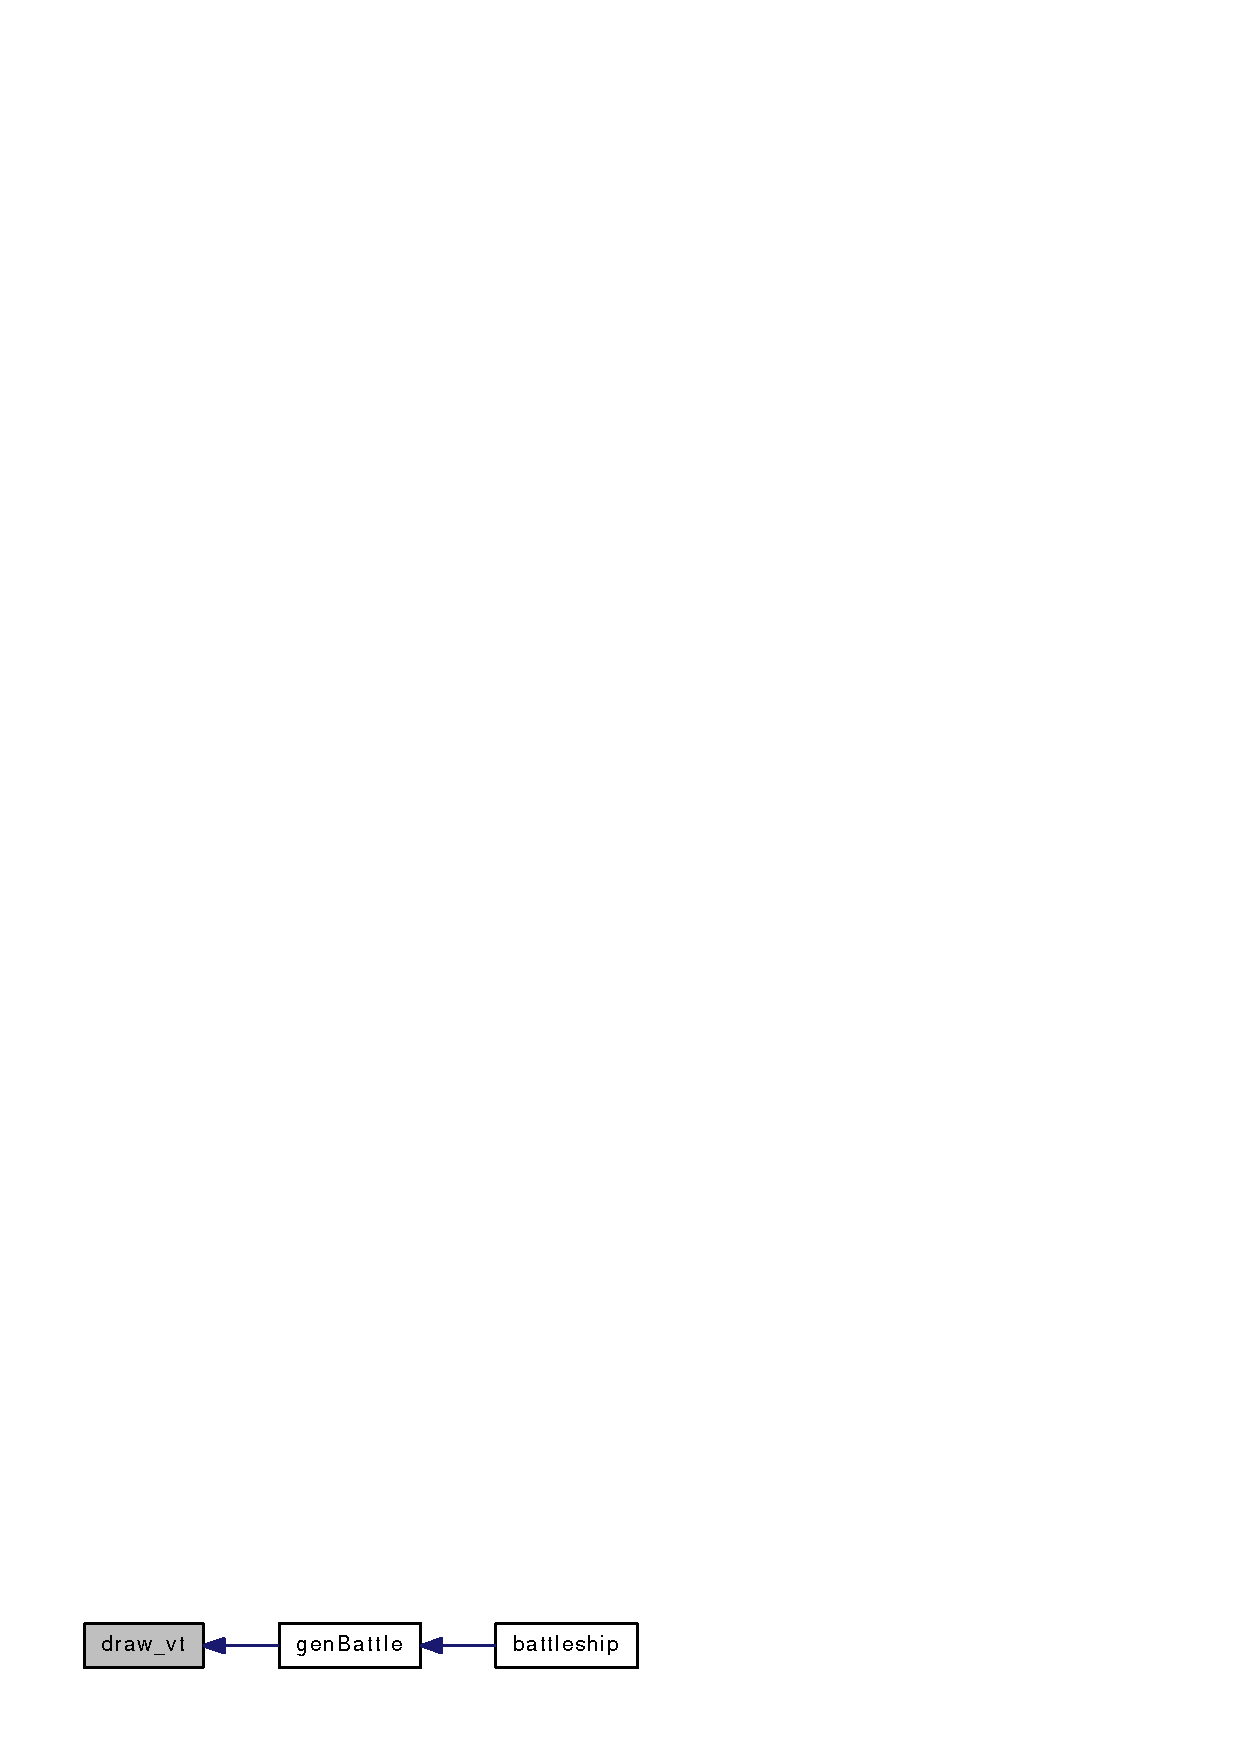
\includegraphics[width=155pt]{bttlship_8h_a2d3705cb0dd809d88cd03e1bb39afb09_icgraph}
\end{center}
\end{figure}


\hypertarget{bttlship_8h_ae442293b5a53448d5a03e47e38396009}{
\index{bttlship.h@{bttlship.h}!genBattle@{genBattle}}
\index{genBattle@{genBattle}!bttlship.h@{bttlship.h}}
\subsubsection[{genBattle}]{\setlength{\rightskip}{0pt plus 5cm}void genBattle ({\bf S\_\-TABLE} $\ast$$\ast$ {\em tableS})}}
\label{bttlship_8h_ae442293b5a53448d5a03e47e38396009}


It generates the table. 


\begin{DoxyParams}{Parameters}
\item[{\em tableS}]The address of the table. \end{DoxyParams}


Definition at line 357 of file bttlship.c.



Here is the call graph for this function:\nopagebreak
\begin{figure}[H]
\begin{center}
\leavevmode
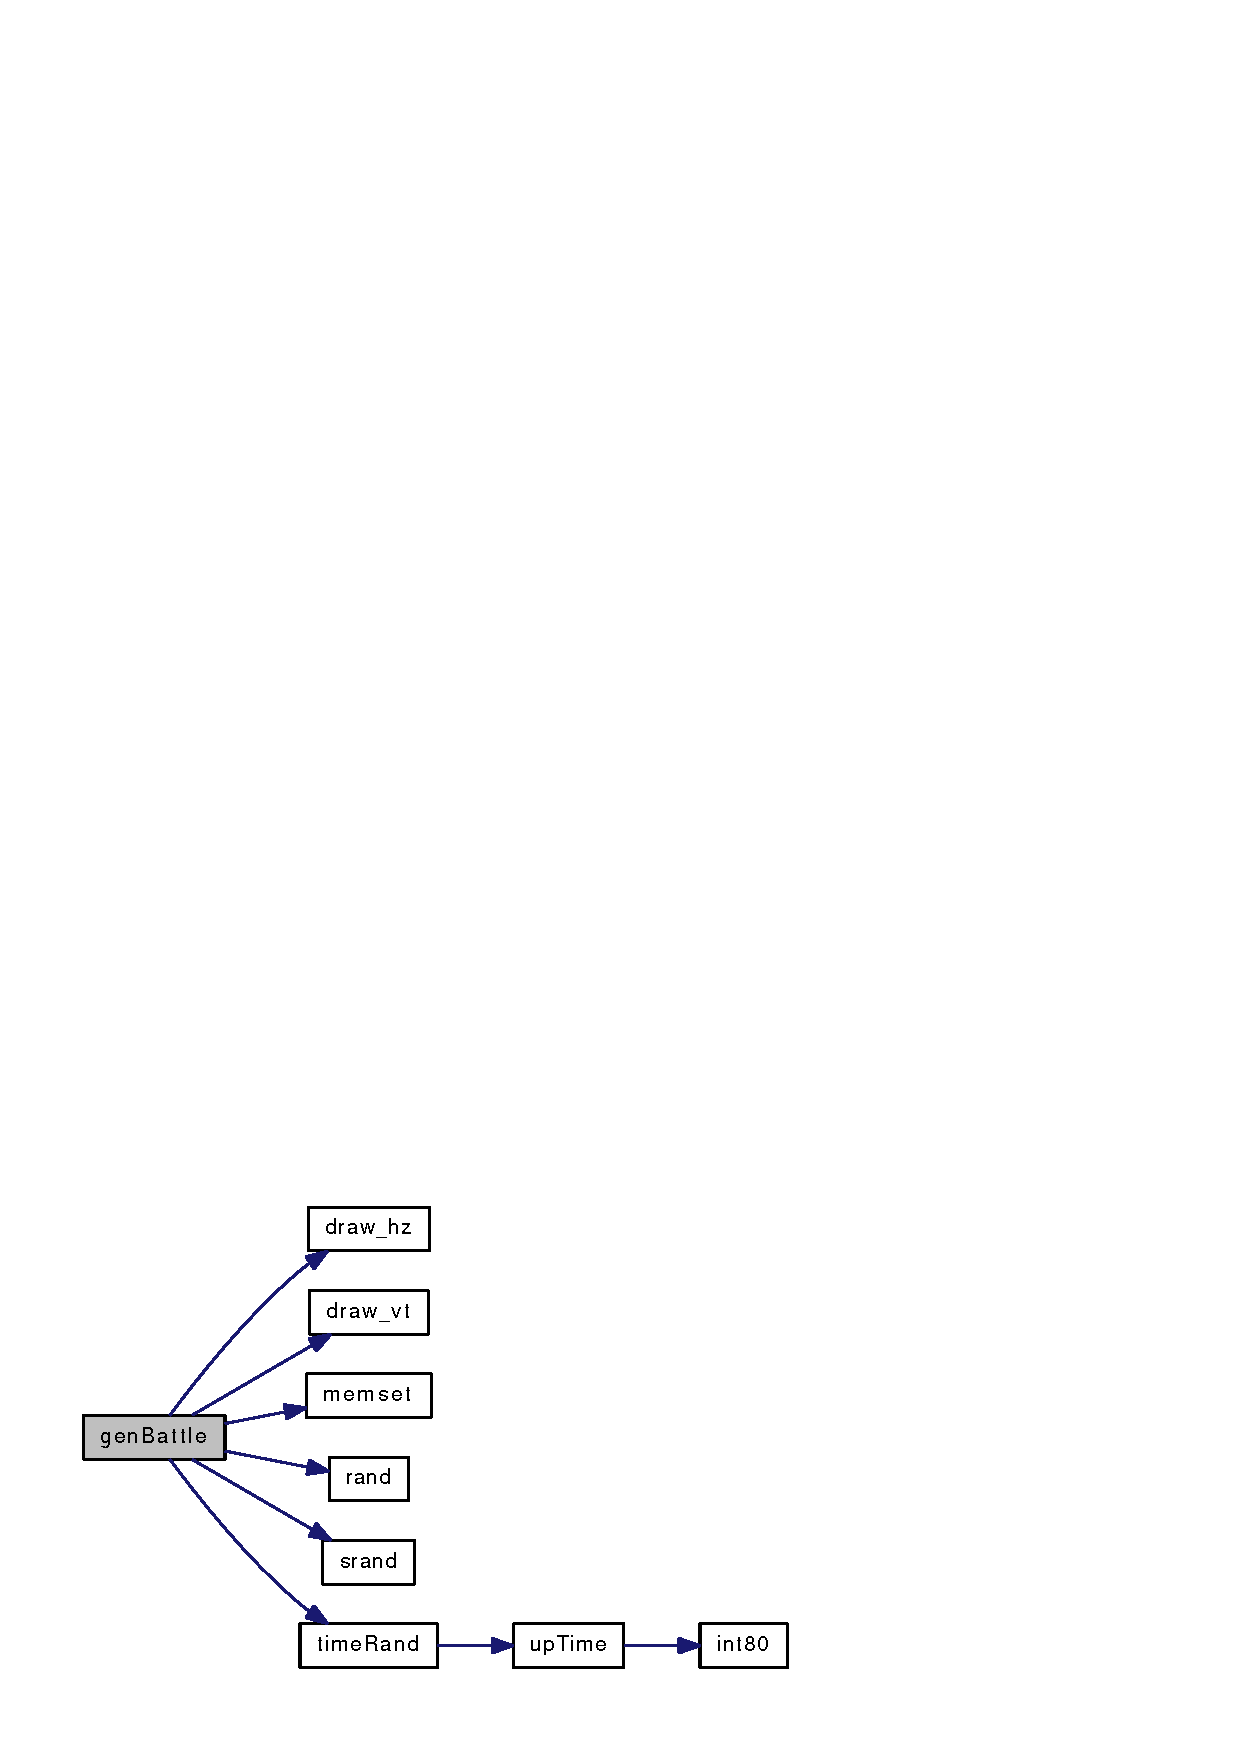
\includegraphics[width=191pt]{bttlship_8h_ae442293b5a53448d5a03e47e38396009_cgraph}
\end{center}
\end{figure}




Here is the caller graph for this function:\nopagebreak
\begin{figure}[H]
\begin{center}
\leavevmode
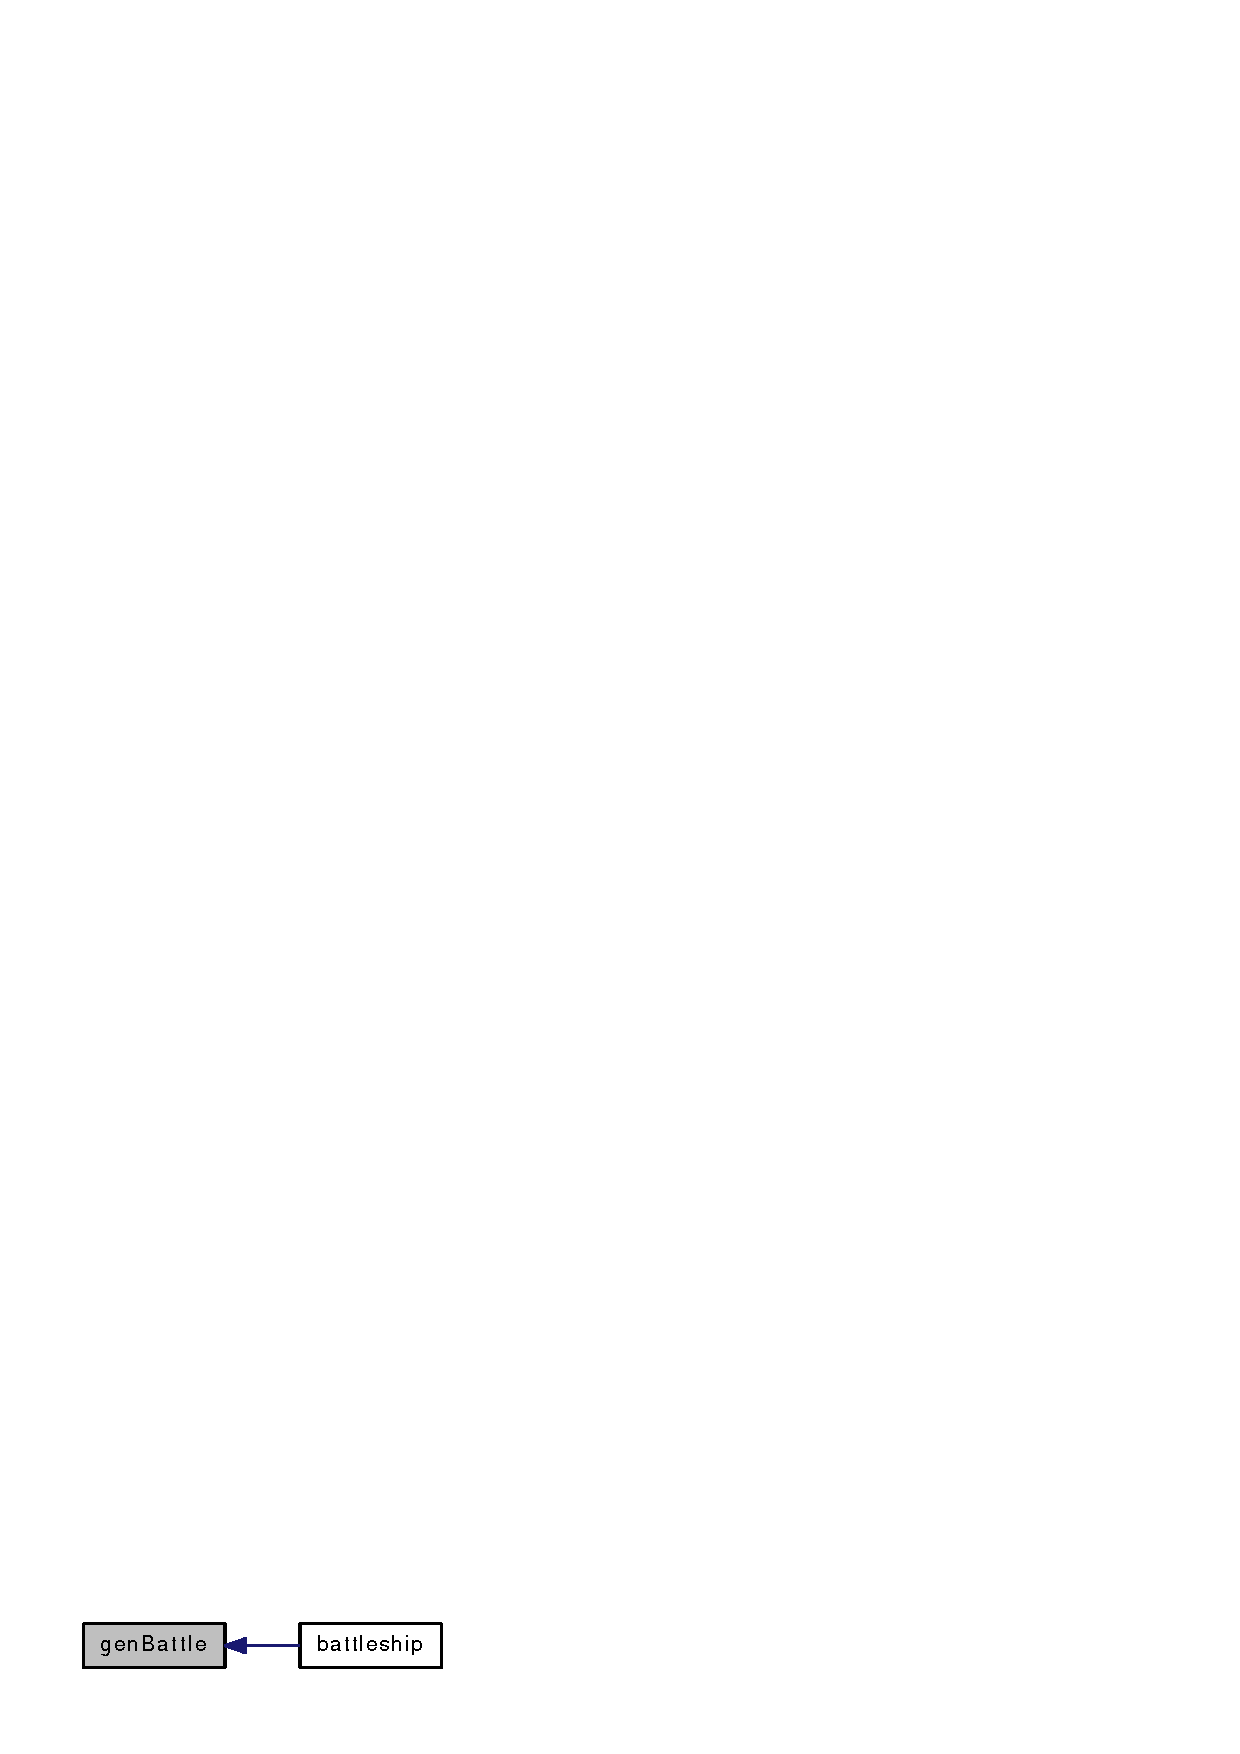
\includegraphics[width=108pt]{bttlship_8h_ae442293b5a53448d5a03e47e38396009_icgraph}
\end{center}
\end{figure}


\hypertarget{bttlship_8h_a4003a14058da5be60c7e7600713cd5c0}{
\index{bttlship.h@{bttlship.h}!getInput@{getInput}}
\index{getInput@{getInput}!bttlship.h@{bttlship.h}}
\subsubsection[{getInput}]{\setlength{\rightskip}{0pt plus 5cm}int getInput (int $\ast$ {\em px}, \/  int $\ast$ {\em py}, \/  {\bf S\_\-TABLE} $\ast$$\ast$ {\em table})}}
\label{bttlship_8h_a4003a14058da5be60c7e7600713cd5c0}


It obtains the the row and the column of the table from STDIN. 


\begin{DoxyParams}{Parameters}
\item[{\em px}]The row of the table \item[{\em py}]The column of the table \item[{\em table}]The address of the table. \end{DoxyParams}


Definition at line 241 of file bttlship.c.



Here is the call graph for this function:\nopagebreak
\begin{figure}[H]
\begin{center}
\leavevmode
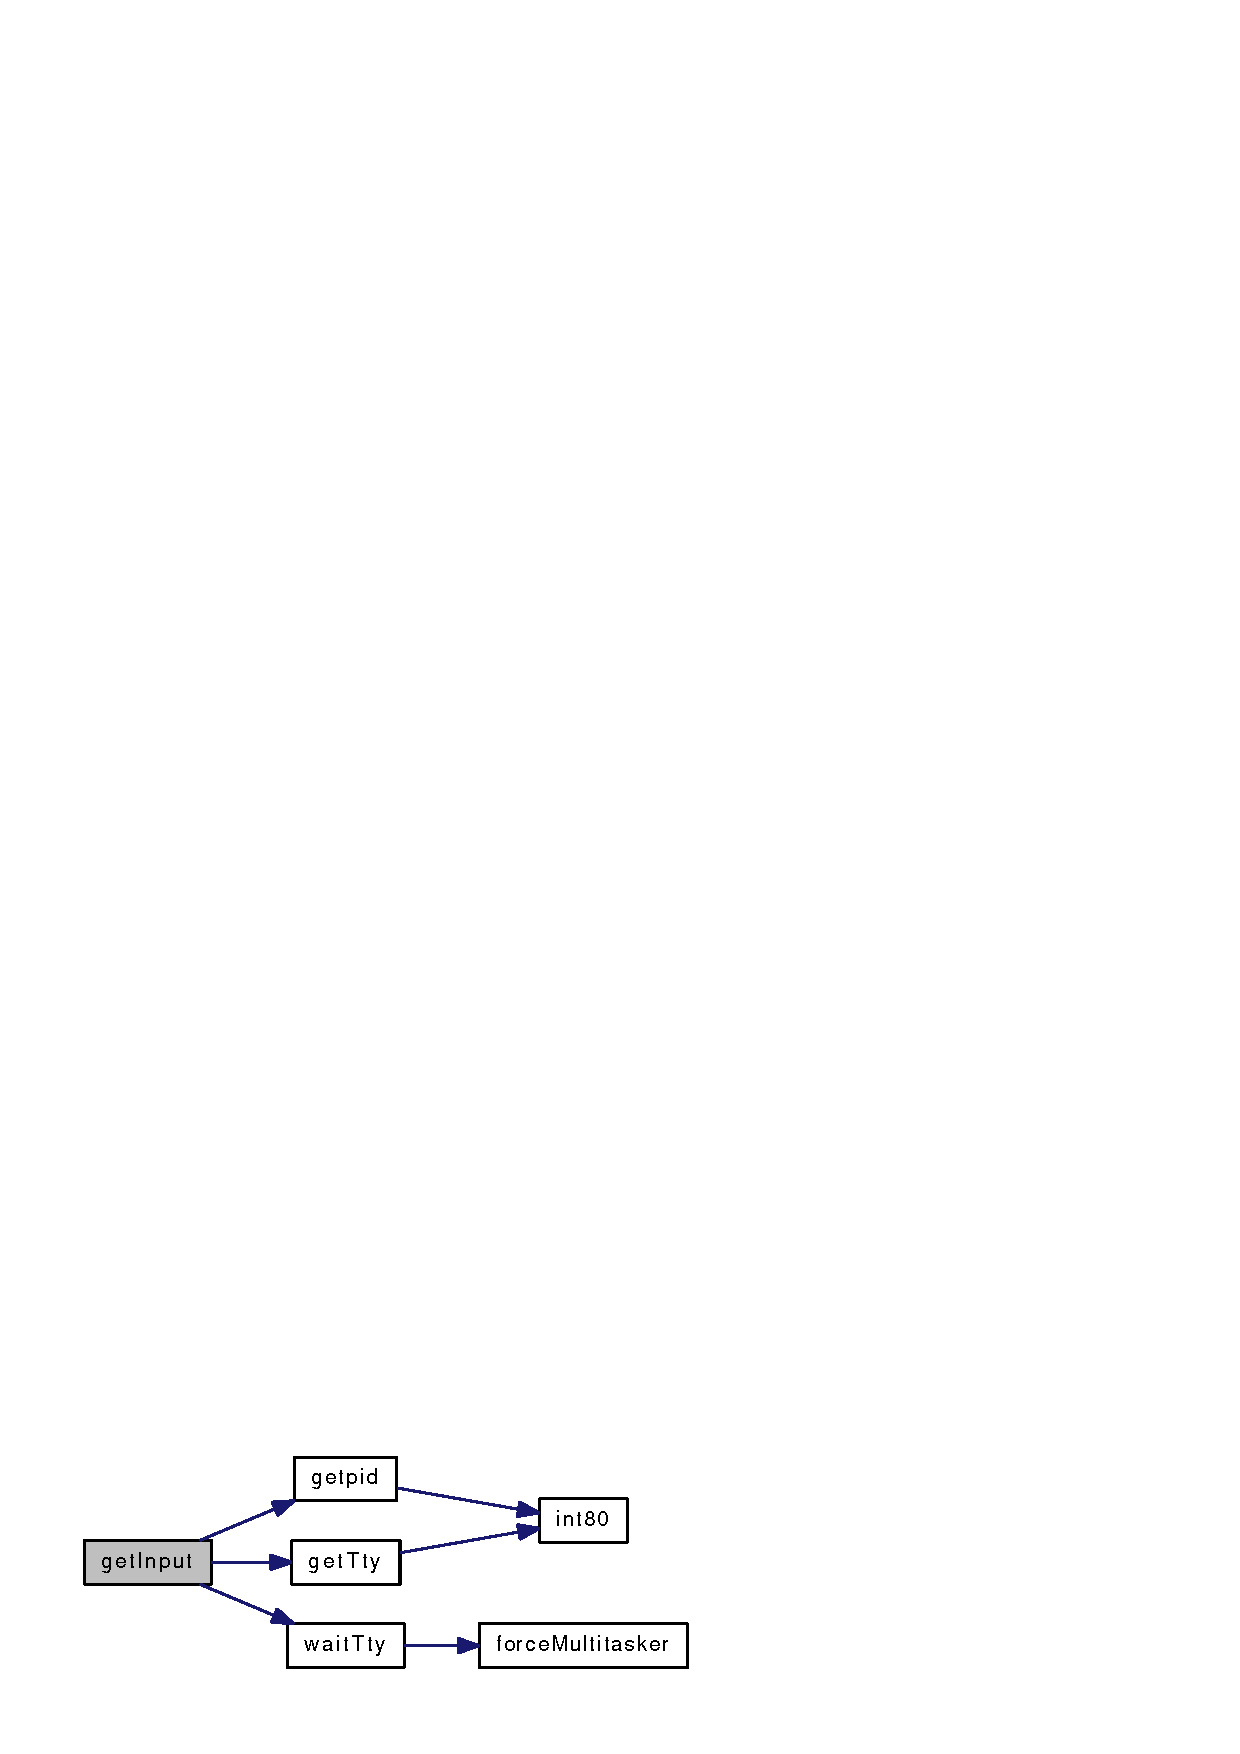
\includegraphics[width=167pt]{bttlship_8h_a4003a14058da5be60c7e7600713cd5c0_cgraph}
\end{center}
\end{figure}




Here is the caller graph for this function:\nopagebreak
\begin{figure}[H]
\begin{center}
\leavevmode
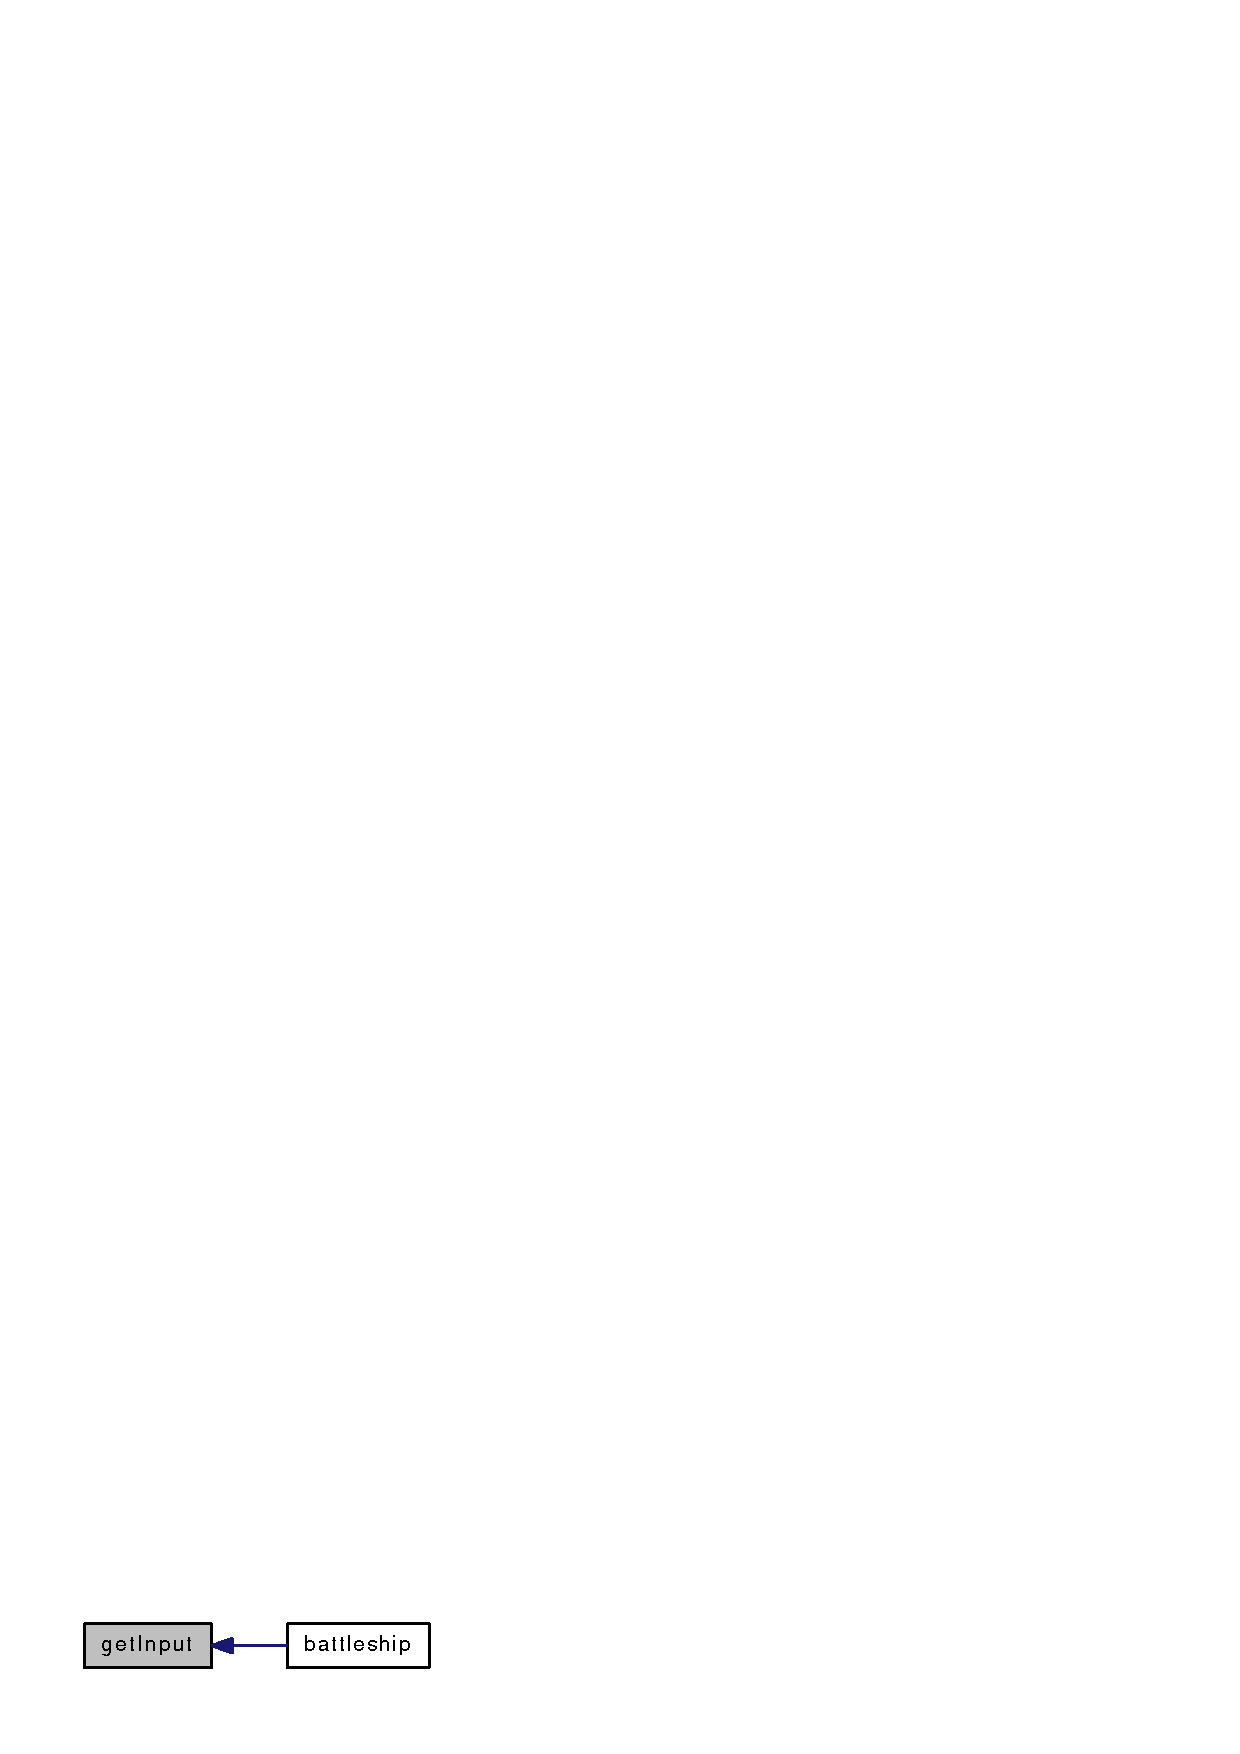
\includegraphics[width=105pt]{bttlship_8h_a4003a14058da5be60c7e7600713cd5c0_icgraph}
\end{center}
\end{figure}


\hypertarget{bttlship_8h_af66d7960a49eb99b5260ba4d524e1ac8}{
\index{bttlship.h@{bttlship.h}!lockTable@{lockTable}}
\index{lockTable@{lockTable}!bttlship.h@{bttlship.h}}
\subsubsection[{lockTable}]{\setlength{\rightskip}{0pt plus 5cm}void lockTable (int {\em semx}, \/  int {\em block}, \/  {\bf S\_\-TABLE} $\ast$$\ast$ {\em tableS})}}
\label{bttlship_8h_af66d7960a49eb99b5260ba4d524e1ac8}


It decides if it has to lock the table or wait for the opponent. Peform semaphore wait/notifies: ARGUMENTS: semx 0 : table lock semaphore 1 : opponent notify semaphore block 0 : perform notify 1 : perform wait. 


\begin{DoxyParams}{Parameters}
\item[{\em semx}]It is the parameter to decide what have to do with semaphore \item[{\em block}]It decides what have to do with the table \item[{\em tableS}]The adress of the table. \end{DoxyParams}


Definition at line 450 of file bttlship.c.



Here is the call graph for this function:\nopagebreak
\begin{figure}[H]
\begin{center}
\leavevmode
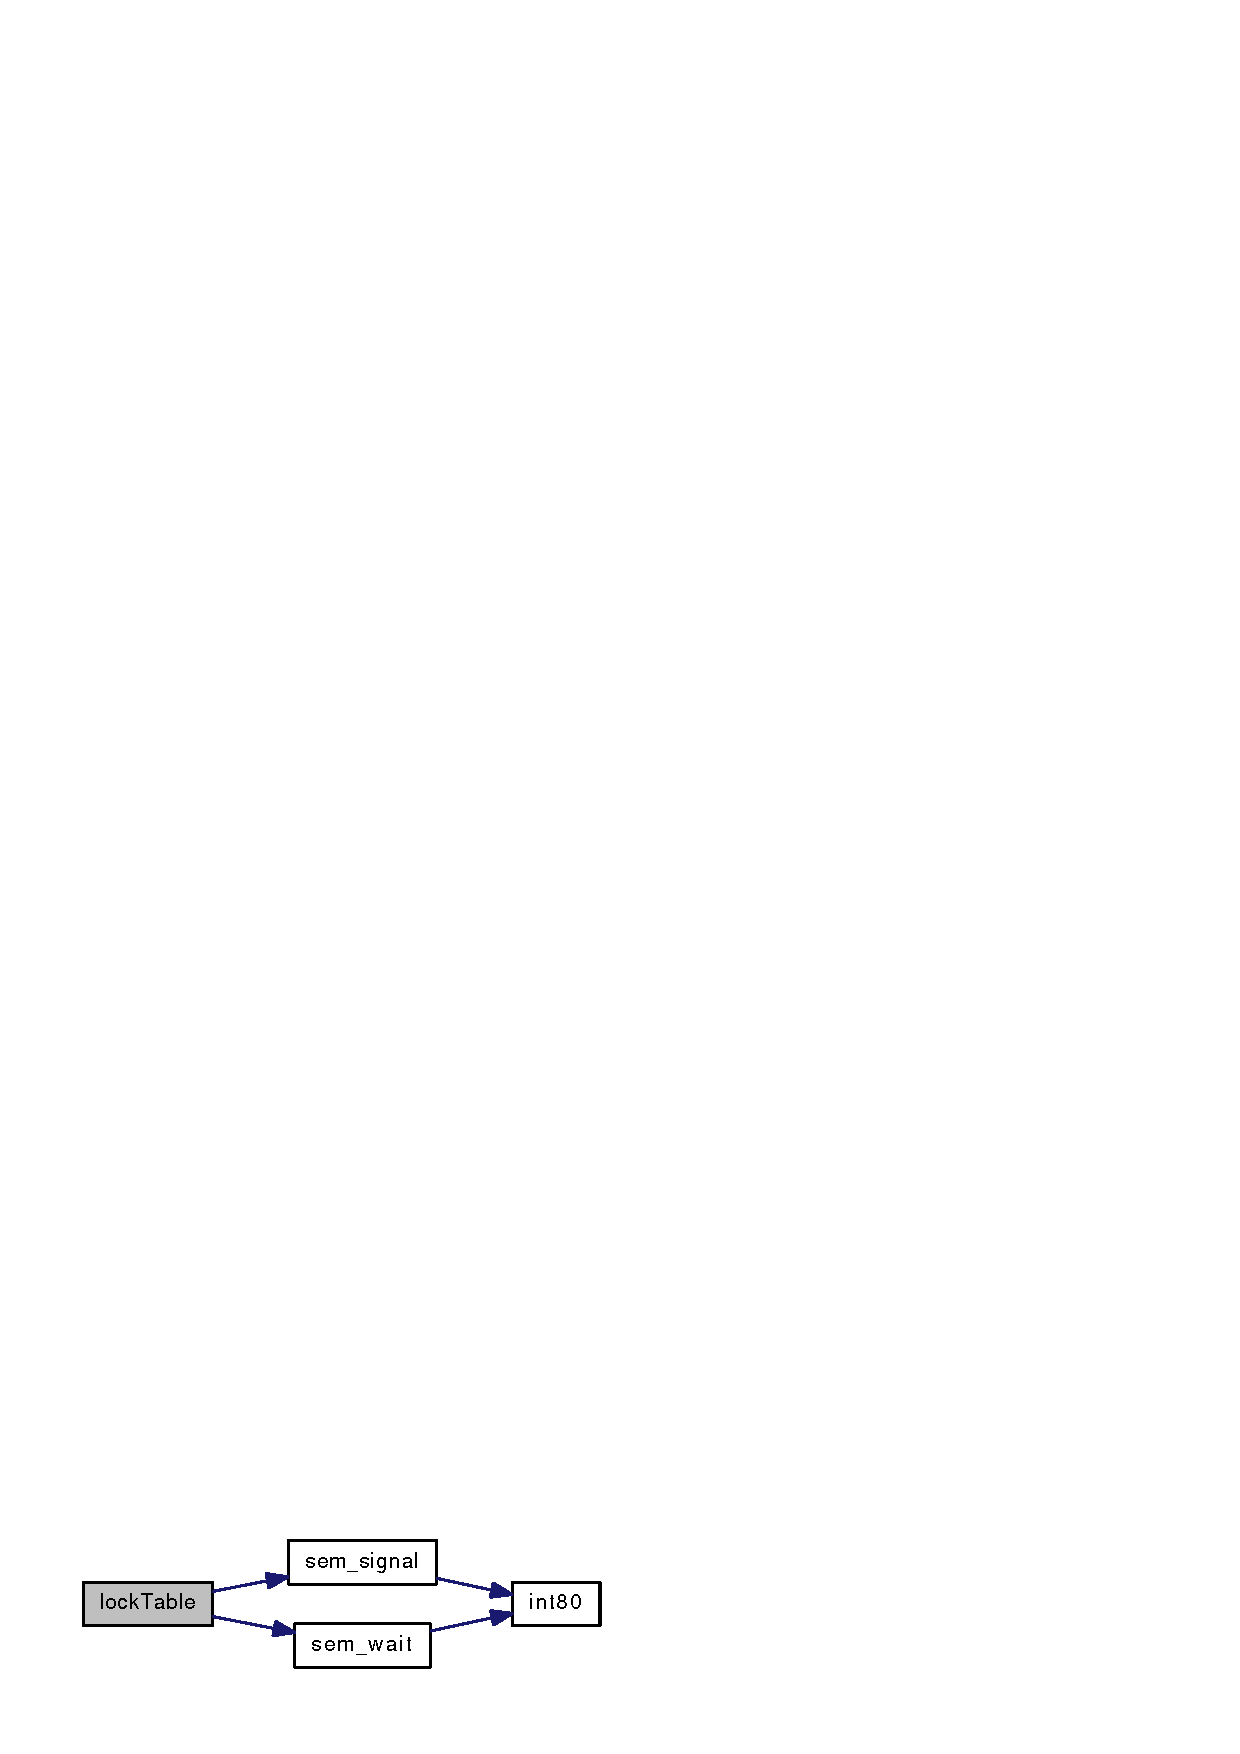
\includegraphics[width=146pt]{bttlship_8h_af66d7960a49eb99b5260ba4d524e1ac8_cgraph}
\end{center}
\end{figure}


\hypertarget{bttlship_8h_a03efcb954008fc3018e19f0353b58157}{
\index{bttlship.h@{bttlship.h}!recount@{recount}}
\index{recount@{recount}!bttlship.h@{bttlship.h}}
\subsubsection[{recount}]{\setlength{\rightskip}{0pt plus 5cm}void recount ({\bf S\_\-TABLE} $\ast$$\ast$ {\em tableS}, \/  int $\ast$ {\em flg\_\-game\_\-over})}}
\label{bttlship_8h_a03efcb954008fc3018e19f0353b58157}


It counts the amount of bombs that the player has left. 


\begin{DoxyParams}{Parameters}
\item[{\em tableS}]The address of the table. \item[{\em flg\_\-game\_\-over}]The adress of the game status. \end{DoxyParams}


Definition at line 210 of file bttlship.c.



Here is the caller graph for this function:\nopagebreak
\begin{figure}[H]
\begin{center}
\leavevmode
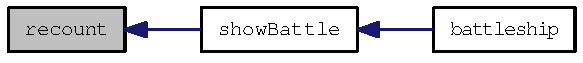
\includegraphics[width=158pt]{bttlship_8h_a03efcb954008fc3018e19f0353b58157_icgraph}
\end{center}
\end{figure}


\hypertarget{bttlship_8h_a21c4f719d9c70f144ffbb7b4ab57d935}{
\index{bttlship.h@{bttlship.h}!showBattle@{showBattle}}
\index{showBattle@{showBattle}!bttlship.h@{bttlship.h}}
\subsubsection[{showBattle}]{\setlength{\rightskip}{0pt plus 5cm}void showBattle ({\bf S\_\-TABLE} $\ast$$\ast$ {\em tableS}, \/  int {\em us}, \/  int {\em them}, \/  int $\ast$ {\em flg\_\-game\_\-over})}}
\label{bttlship_8h_a21c4f719d9c70f144ffbb7b4ab57d935}


It prints the table of the battlehsip. 


\begin{DoxyParams}{Parameters}
\item[{\em tableS}]The address of the table. \item[{\em us}]Inner use. \item[{\em them}]Inner use. \item[{\em flg\_\-game\_\-over}]The address of the game status. \end{DoxyParams}


Definition at line 400 of file bttlship.c.



Here is the call graph for this function:\nopagebreak
\begin{figure}[H]
\begin{center}
\leavevmode
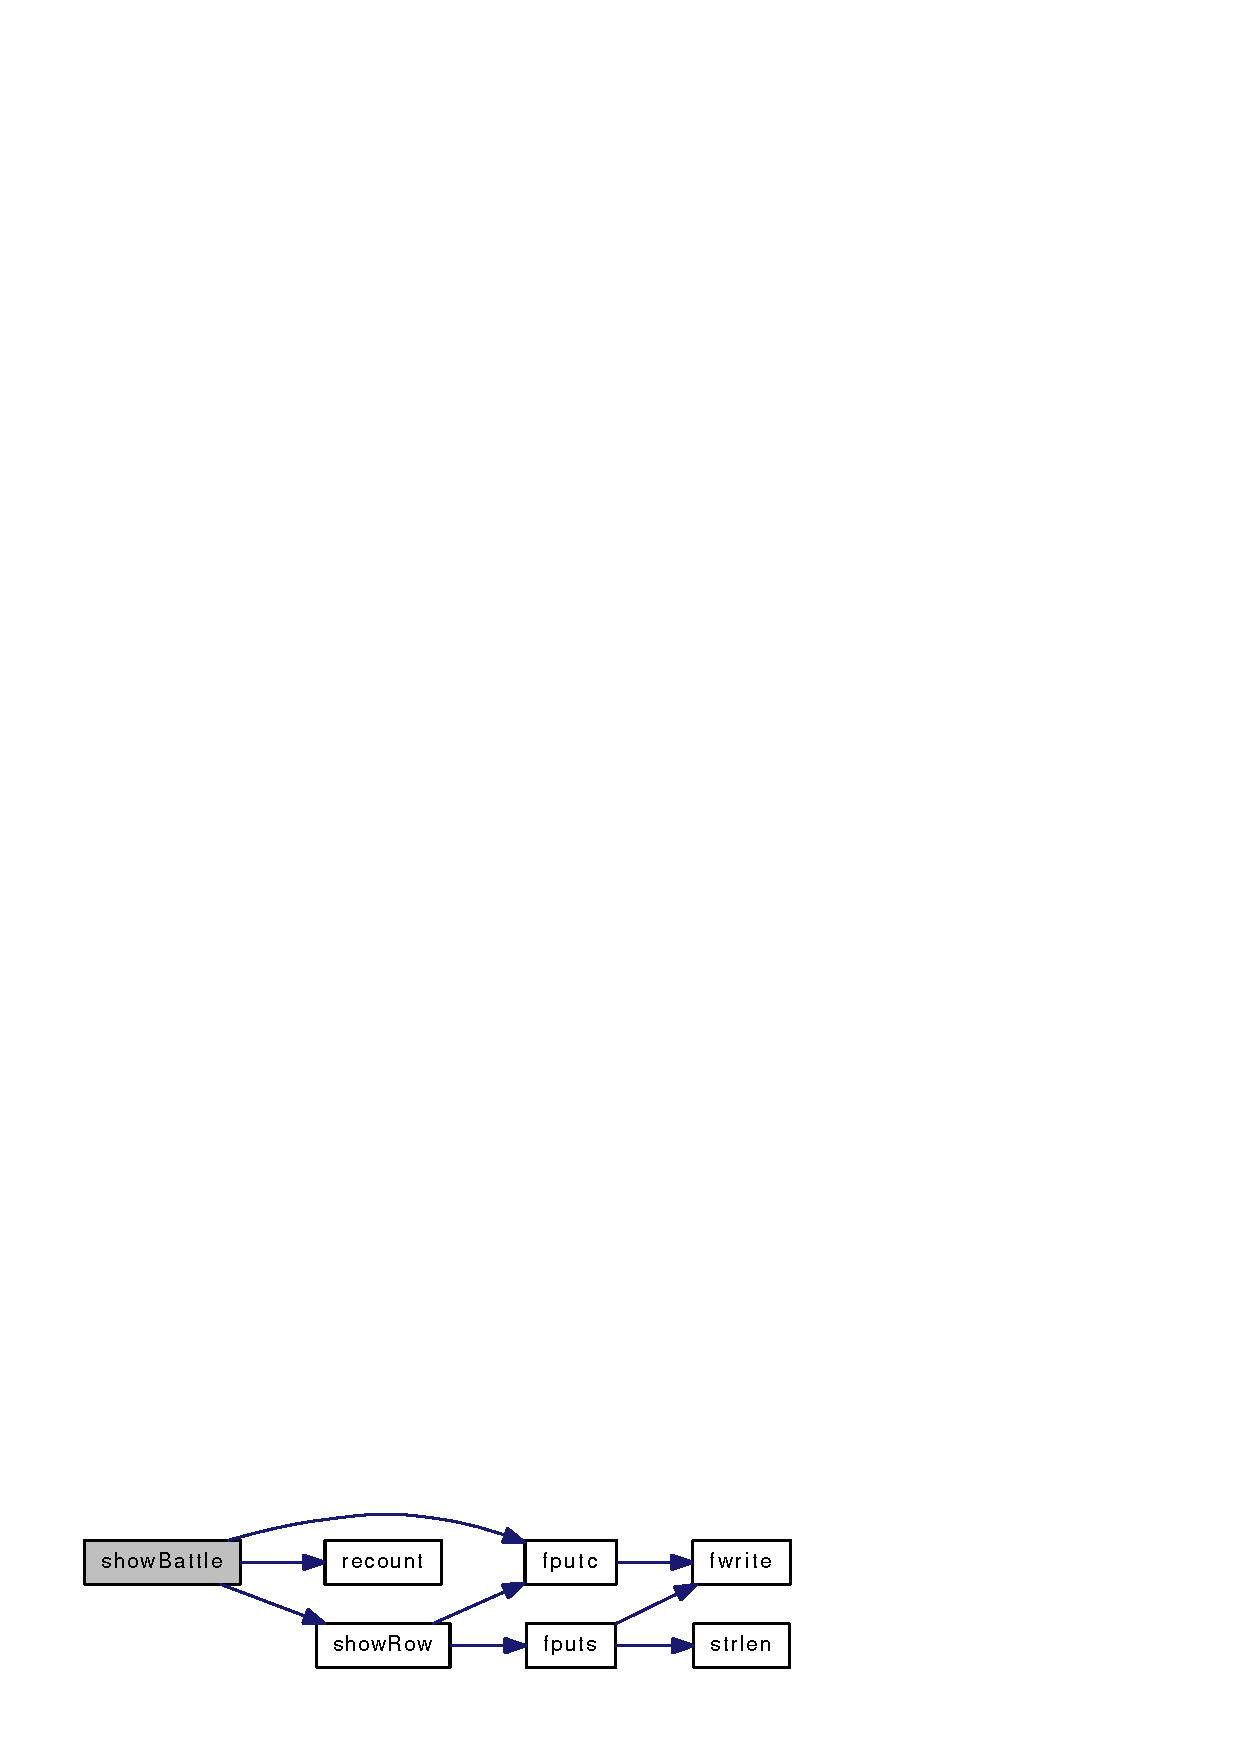
\includegraphics[width=192pt]{bttlship_8h_a21c4f719d9c70f144ffbb7b4ab57d935_cgraph}
\end{center}
\end{figure}




Here is the caller graph for this function:\nopagebreak
\begin{figure}[H]
\begin{center}
\leavevmode
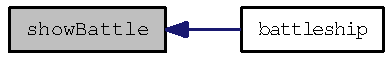
\includegraphics[width=112pt]{bttlship_8h_a21c4f719d9c70f144ffbb7b4ab57d935_icgraph}
\end{center}
\end{figure}


\hypertarget{bttlship_8h_afcb21d332942ec61fd523fed20b758e5}{
\index{bttlship.h@{bttlship.h}!showRow@{showRow}}
\index{showRow@{showRow}!bttlship.h@{bttlship.h}}
\subsubsection[{showRow}]{\setlength{\rightskip}{0pt plus 5cm}void showRow (void)}}
\label{bttlship_8h_afcb21d332942ec61fd523fed20b758e5}


It prints each row of the table. 



Definition at line 389 of file bttlship.c.



Here is the call graph for this function:\nopagebreak
\begin{figure}[H]
\begin{center}
\leavevmode
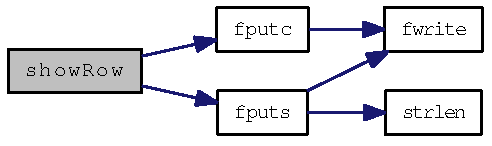
\includegraphics[width=136pt]{bttlship_8h_afcb21d332942ec61fd523fed20b758e5_cgraph}
\end{center}
\end{figure}




Here is the caller graph for this function:\nopagebreak
\begin{figure}[H]
\begin{center}
\leavevmode
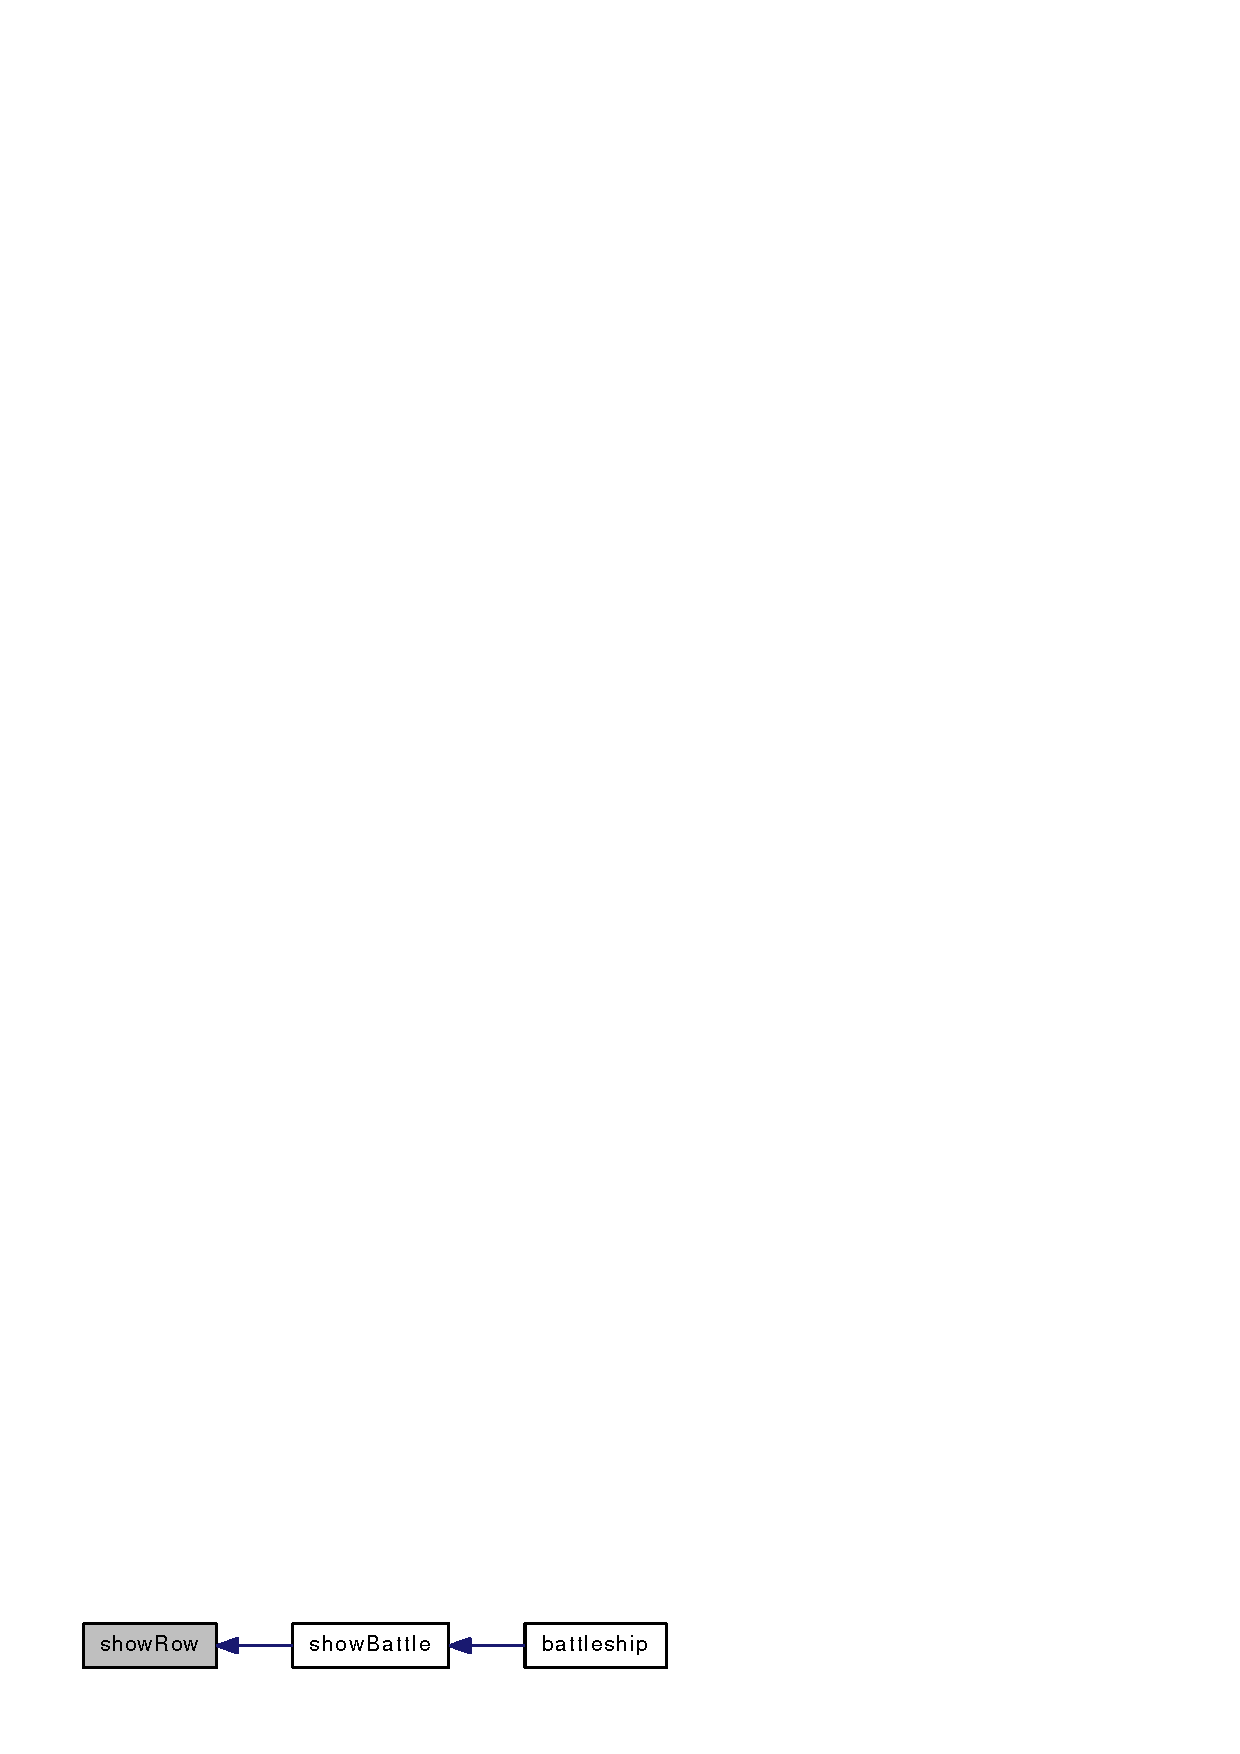
\includegraphics[width=162pt]{bttlship_8h_afcb21d332942ec61fd523fed20b758e5_icgraph}
\end{center}
\end{figure}



\hypertarget{colors_8h}{
\section{inc/colors.h File Reference}
\label{colors_8h}\index{inc/colors.h@{inc/colors.h}}
}


Video Color defines.  


This graph shows which files directly or indirectly include this file:\nopagebreak
\begin{figure}[H]
\begin{center}
\leavevmode
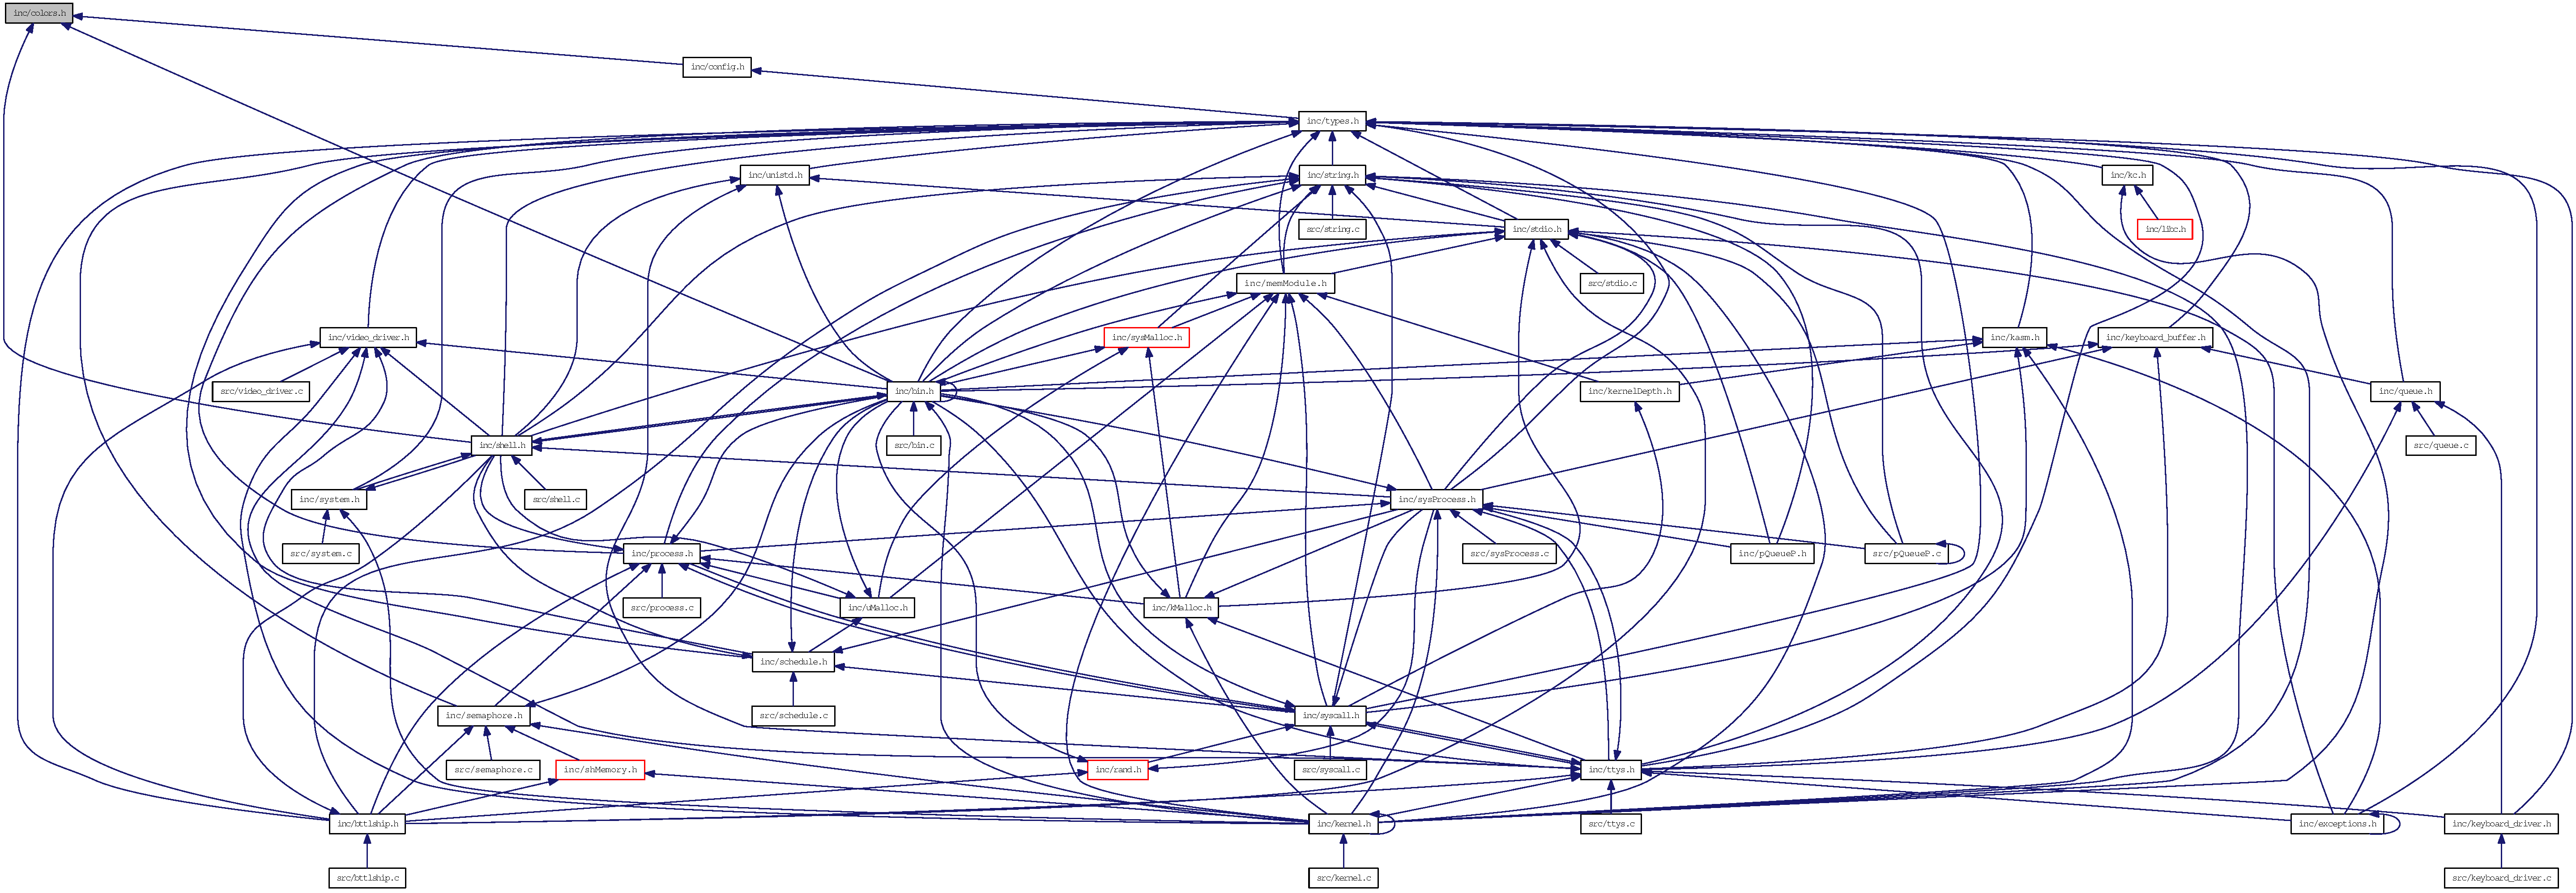
\includegraphics[width=420pt]{colors_8h__dep__incl}
\end{center}
\end{figure}
\subsection*{Defines}
\begin{DoxyCompactItemize}
\item 
\#define \hyperlink{colors_8h_a7b3b25cba33b07c303f3060fe41887f6}{BLACK}~0x0
\item 
\#define \hyperlink{colors_8h_a79d10e672abb49ad63eeaa8aaef57c38}{BLUE}~0x1
\item 
\#define \hyperlink{colors_8h_acfbc006ea433ad708fdee3e82996e721}{GREEN}~0x2
\item 
\#define \hyperlink{colors_8h_ad243f93c16bc4c1d3e0a13b84421d760}{CYAN}~0x3
\item 
\#define \hyperlink{colors_8h_a8d23feea868a983c8c2b661e1e16972f}{RED}~0x4
\item 
\#define \hyperlink{colors_8h_a6f699060902f800f12aaae150f3a708e}{MAGENTA}~0x5
\item 
\#define \hyperlink{colors_8h_ab2baea56ece91306020afd6d77fd19f9}{BROWN}~0x6
\item 
\#define \hyperlink{colors_8h_acafbbc051d018cffe2fcddcbf778c304}{LIGHT\_\-GREY}~0x7
\item 
\#define \hyperlink{colors_8h_a85998c833c5007dc61315ea69919582e}{DARK\_\-GREY}~0x8
\item 
\#define \hyperlink{colors_8h_a959d1249a76cfbd90fc6d96e2a9744e9}{LIGHT\_\-BLUE}~0x9
\item 
\#define \hyperlink{colors_8h_a5a7142ee95ebc63218ed3aac2ae06b13}{LIGHT\_\-GREEN}~0xA
\item 
\#define \hyperlink{colors_8h_a15e616ad647add2891b6c7ec6a1e47f1}{LIGHT\_\-CYAN}~0xB
\item 
\#define \hyperlink{colors_8h_a664c8f5b9d90f79a49a16960b9ccedba}{LIGHT\_\-RED}~0xC
\item 
\#define \hyperlink{colors_8h_af98a47a241abb10ccec0339c7a8a8c2e}{LIGHT\_\-MAGENTA}~0xD
\item 
\#define \hyperlink{colors_8h_a8ed224d3e366a4c3b718a44146075446}{LIGHT\_\-BROWN}~0xE
\item 
\#define \hyperlink{colors_8h_a87b537f5fa5c109d3c05c13d6b18f382}{WHITE}~0xF
\item 
\#define \hyperlink{colors_8h_a587223a5cf6a783335c29a47bec92155}{setColor}(bkg, text)~(((bkg) $<$$<$ 4) + (text))
\end{DoxyCompactItemize}


\subsection{Detailed Description}
Video Color defines. \begin{DoxyAuthor}{Author}
Luciano Zemin, Nicolás Magni, Nicolás Purita 
\end{DoxyAuthor}


Definition in file \hyperlink{colors_8h_source}{colors.h}.



\subsection{Define Documentation}
\hypertarget{colors_8h_a7b3b25cba33b07c303f3060fe41887f6}{
\index{colors.h@{colors.h}!BLACK@{BLACK}}
\index{BLACK@{BLACK}!colors.h@{colors.h}}
\subsubsection[{BLACK}]{\setlength{\rightskip}{0pt plus 5cm}\#define BLACK~0x0}}
\label{colors_8h_a7b3b25cba33b07c303f3060fe41887f6}


Definition at line 13 of file colors.h.

\hypertarget{colors_8h_a79d10e672abb49ad63eeaa8aaef57c38}{
\index{colors.h@{colors.h}!BLUE@{BLUE}}
\index{BLUE@{BLUE}!colors.h@{colors.h}}
\subsubsection[{BLUE}]{\setlength{\rightskip}{0pt plus 5cm}\#define BLUE~0x1}}
\label{colors_8h_a79d10e672abb49ad63eeaa8aaef57c38}


Definition at line 14 of file colors.h.

\hypertarget{colors_8h_ab2baea56ece91306020afd6d77fd19f9}{
\index{colors.h@{colors.h}!BROWN@{BROWN}}
\index{BROWN@{BROWN}!colors.h@{colors.h}}
\subsubsection[{BROWN}]{\setlength{\rightskip}{0pt plus 5cm}\#define BROWN~0x6}}
\label{colors_8h_ab2baea56ece91306020afd6d77fd19f9}


Definition at line 19 of file colors.h.

\hypertarget{colors_8h_ad243f93c16bc4c1d3e0a13b84421d760}{
\index{colors.h@{colors.h}!CYAN@{CYAN}}
\index{CYAN@{CYAN}!colors.h@{colors.h}}
\subsubsection[{CYAN}]{\setlength{\rightskip}{0pt plus 5cm}\#define CYAN~0x3}}
\label{colors_8h_ad243f93c16bc4c1d3e0a13b84421d760}


Definition at line 16 of file colors.h.

\hypertarget{colors_8h_a85998c833c5007dc61315ea69919582e}{
\index{colors.h@{colors.h}!DARK\_\-GREY@{DARK\_\-GREY}}
\index{DARK\_\-GREY@{DARK\_\-GREY}!colors.h@{colors.h}}
\subsubsection[{DARK\_\-GREY}]{\setlength{\rightskip}{0pt plus 5cm}\#define DARK\_\-GREY~0x8}}
\label{colors_8h_a85998c833c5007dc61315ea69919582e}


Definition at line 21 of file colors.h.

\hypertarget{colors_8h_acfbc006ea433ad708fdee3e82996e721}{
\index{colors.h@{colors.h}!GREEN@{GREEN}}
\index{GREEN@{GREEN}!colors.h@{colors.h}}
\subsubsection[{GREEN}]{\setlength{\rightskip}{0pt plus 5cm}\#define GREEN~0x2}}
\label{colors_8h_acfbc006ea433ad708fdee3e82996e721}


Definition at line 15 of file colors.h.

\hypertarget{colors_8h_a959d1249a76cfbd90fc6d96e2a9744e9}{
\index{colors.h@{colors.h}!LIGHT\_\-BLUE@{LIGHT\_\-BLUE}}
\index{LIGHT\_\-BLUE@{LIGHT\_\-BLUE}!colors.h@{colors.h}}
\subsubsection[{LIGHT\_\-BLUE}]{\setlength{\rightskip}{0pt plus 5cm}\#define LIGHT\_\-BLUE~0x9}}
\label{colors_8h_a959d1249a76cfbd90fc6d96e2a9744e9}


Definition at line 22 of file colors.h.

\hypertarget{colors_8h_a8ed224d3e366a4c3b718a44146075446}{
\index{colors.h@{colors.h}!LIGHT\_\-BROWN@{LIGHT\_\-BROWN}}
\index{LIGHT\_\-BROWN@{LIGHT\_\-BROWN}!colors.h@{colors.h}}
\subsubsection[{LIGHT\_\-BROWN}]{\setlength{\rightskip}{0pt plus 5cm}\#define LIGHT\_\-BROWN~0xE}}
\label{colors_8h_a8ed224d3e366a4c3b718a44146075446}


Definition at line 27 of file colors.h.

\hypertarget{colors_8h_a15e616ad647add2891b6c7ec6a1e47f1}{
\index{colors.h@{colors.h}!LIGHT\_\-CYAN@{LIGHT\_\-CYAN}}
\index{LIGHT\_\-CYAN@{LIGHT\_\-CYAN}!colors.h@{colors.h}}
\subsubsection[{LIGHT\_\-CYAN}]{\setlength{\rightskip}{0pt plus 5cm}\#define LIGHT\_\-CYAN~0xB}}
\label{colors_8h_a15e616ad647add2891b6c7ec6a1e47f1}


Definition at line 24 of file colors.h.

\hypertarget{colors_8h_a5a7142ee95ebc63218ed3aac2ae06b13}{
\index{colors.h@{colors.h}!LIGHT\_\-GREEN@{LIGHT\_\-GREEN}}
\index{LIGHT\_\-GREEN@{LIGHT\_\-GREEN}!colors.h@{colors.h}}
\subsubsection[{LIGHT\_\-GREEN}]{\setlength{\rightskip}{0pt plus 5cm}\#define LIGHT\_\-GREEN~0xA}}
\label{colors_8h_a5a7142ee95ebc63218ed3aac2ae06b13}


Definition at line 23 of file colors.h.

\hypertarget{colors_8h_acafbbc051d018cffe2fcddcbf778c304}{
\index{colors.h@{colors.h}!LIGHT\_\-GREY@{LIGHT\_\-GREY}}
\index{LIGHT\_\-GREY@{LIGHT\_\-GREY}!colors.h@{colors.h}}
\subsubsection[{LIGHT\_\-GREY}]{\setlength{\rightskip}{0pt plus 5cm}\#define LIGHT\_\-GREY~0x7}}
\label{colors_8h_acafbbc051d018cffe2fcddcbf778c304}


Definition at line 20 of file colors.h.

\hypertarget{colors_8h_af98a47a241abb10ccec0339c7a8a8c2e}{
\index{colors.h@{colors.h}!LIGHT\_\-MAGENTA@{LIGHT\_\-MAGENTA}}
\index{LIGHT\_\-MAGENTA@{LIGHT\_\-MAGENTA}!colors.h@{colors.h}}
\subsubsection[{LIGHT\_\-MAGENTA}]{\setlength{\rightskip}{0pt plus 5cm}\#define LIGHT\_\-MAGENTA~0xD}}
\label{colors_8h_af98a47a241abb10ccec0339c7a8a8c2e}


Definition at line 26 of file colors.h.

\hypertarget{colors_8h_a664c8f5b9d90f79a49a16960b9ccedba}{
\index{colors.h@{colors.h}!LIGHT\_\-RED@{LIGHT\_\-RED}}
\index{LIGHT\_\-RED@{LIGHT\_\-RED}!colors.h@{colors.h}}
\subsubsection[{LIGHT\_\-RED}]{\setlength{\rightskip}{0pt plus 5cm}\#define LIGHT\_\-RED~0xC}}
\label{colors_8h_a664c8f5b9d90f79a49a16960b9ccedba}


Definition at line 25 of file colors.h.

\hypertarget{colors_8h_a6f699060902f800f12aaae150f3a708e}{
\index{colors.h@{colors.h}!MAGENTA@{MAGENTA}}
\index{MAGENTA@{MAGENTA}!colors.h@{colors.h}}
\subsubsection[{MAGENTA}]{\setlength{\rightskip}{0pt plus 5cm}\#define MAGENTA~0x5}}
\label{colors_8h_a6f699060902f800f12aaae150f3a708e}


Definition at line 18 of file colors.h.

\hypertarget{colors_8h_a8d23feea868a983c8c2b661e1e16972f}{
\index{colors.h@{colors.h}!RED@{RED}}
\index{RED@{RED}!colors.h@{colors.h}}
\subsubsection[{RED}]{\setlength{\rightskip}{0pt plus 5cm}\#define RED~0x4}}
\label{colors_8h_a8d23feea868a983c8c2b661e1e16972f}


Definition at line 17 of file colors.h.

\hypertarget{colors_8h_a587223a5cf6a783335c29a47bec92155}{
\index{colors.h@{colors.h}!setColor@{setColor}}
\index{setColor@{setColor}!colors.h@{colors.h}}
\subsubsection[{setColor}]{\setlength{\rightskip}{0pt plus 5cm}\#define setColor(bkg, \/  text)~(((bkg) $<$$<$ 4) + (text))}}
\label{colors_8h_a587223a5cf6a783335c29a47bec92155}


Definition at line 30 of file colors.h.

\hypertarget{colors_8h_a87b537f5fa5c109d3c05c13d6b18f382}{
\index{colors.h@{colors.h}!WHITE@{WHITE}}
\index{WHITE@{WHITE}!colors.h@{colors.h}}
\subsubsection[{WHITE}]{\setlength{\rightskip}{0pt plus 5cm}\#define WHITE~0xF}}
\label{colors_8h_a87b537f5fa5c109d3c05c13d6b18f382}


Definition at line 28 of file colors.h.


\hypertarget{config_8h}{
\section{inc/config.h File Reference}
\label{config_8h}\index{inc/config.h@{inc/config.h}}
}


OS configuration defines.  


{\ttfamily \#include \char`\"{}colors.h\char`\"{}}\par
Include dependency graph for config.h:\nopagebreak
\begin{figure}[H]
\begin{center}
\leavevmode
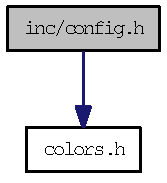
\includegraphics[width=58pt]{config_8h__incl}
\end{center}
\end{figure}
This graph shows which files directly or indirectly include this file:\nopagebreak
\begin{figure}[H]
\begin{center}
\leavevmode
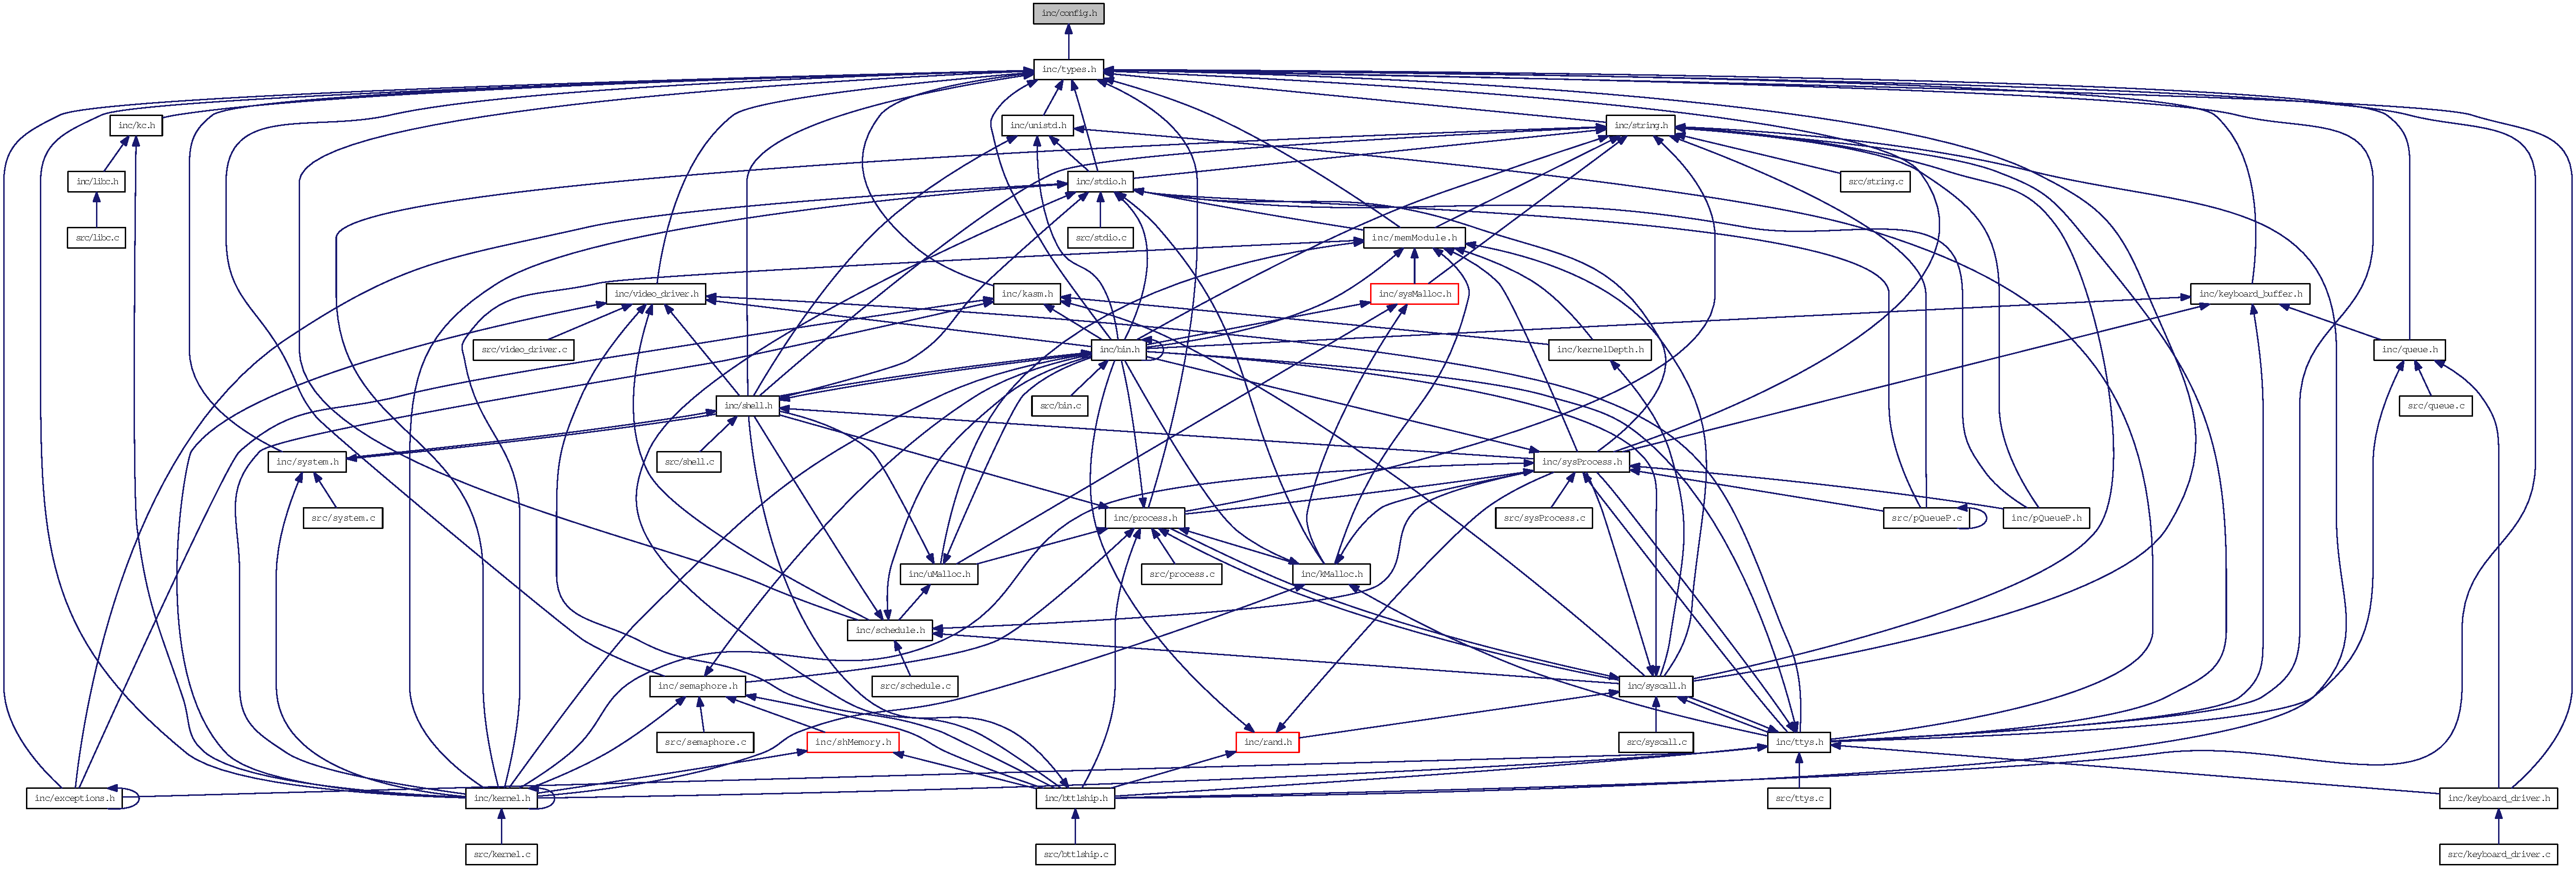
\includegraphics[width=420pt]{config_8h__dep__incl}
\end{center}
\end{figure}
\subsection*{Defines}
\begin{DoxyCompactItemize}
\item 
\#define \hyperlink{config_8h_a2cd109632a6dcccaa80b43561b1ab700}{SCREEN\_\-WIDTH}~80
\begin{DoxyCompactList}\small\item\em The width of the screen. \item\end{DoxyCompactList}\item 
\#define \hyperlink{config_8h_a25f7ae536603397e929ff4941e253200}{SCREEN\_\-HEIGTH}~25
\begin{DoxyCompactList}\small\item\em The height of the screen. \item\end{DoxyCompactList}\item 
\#define \hyperlink{config_8h_a6cacb150853456c97c51481e67d0dabc}{SCREEN\_\-SIZE}~SCREEN\_\-WIDTH $\ast$ SCREEN\_\-HEIGTH
\begin{DoxyCompactList}\small\item\em Real screen size without color attribute. \item\end{DoxyCompactList}\item 
\#define \hyperlink{config_8h_a6f784c53fe46a1d7cc4979a97ce2b484}{VIDEO\_\-MEMORY\_\-SIZE}~SCREEN\_\-SIZE $\ast$ 2
\begin{DoxyCompactList}\small\item\em Real screen size with color attributes. \item\end{DoxyCompactList}\item 
\#define \hyperlink{config_8h_a96df1fa5a1eb0452e87bad701a632eeb}{CURSOR\_\-START\_\-COL}~0
\begin{DoxyCompactList}\small\item\em The starter column position. \item\end{DoxyCompactList}\item 
\#define \hyperlink{config_8h_a0918341b64efcf251a70fc2c188803fa}{CURSOR\_\-START\_\-ROW}~0
\begin{DoxyCompactList}\small\item\em The starter row position. \item\end{DoxyCompactList}\item 
\#define \hyperlink{config_8h_a625199558fb05110496080e008423fa6}{VIDEO\_\-TAB\_\-STOP}~4
\begin{DoxyCompactList}\small\item\em The spaces that tab prints. \item\end{DoxyCompactList}\item 
\#define \hyperlink{config_8h_a1a24019cfbf00c9425f1aefb18421453}{VIDEO\_\-VTAB\_\-STOP}~4
\begin{DoxyCompactList}\small\item\em The vertical tab spaces. \item\end{DoxyCompactList}\item 
\#define \hyperlink{config_8h_a4a96c64dbab22978dda9bbf3a52a9fb7}{CURSOR\_\-START\_\-VISIBLE}~1
\begin{DoxyCompactList}\small\item\em The state of the cursor, Visible = 1 v NotVisible = 0. \item\end{DoxyCompactList}\item 
\#define \hyperlink{config_8h_a6a82449f6eb7ef9870e64a127e068485}{VIDEO\_\-COLOR}~setColor(BLACK, WHITE)
\begin{DoxyCompactList}\small\item\em Set color of letters and screen. \item\end{DoxyCompactList}\item 
\#define \hyperlink{config_8h_a4a2e75965162f8faca7c6ab73c98d5bd}{KEYBOARD\_\-REPETITION}~3
\begin{DoxyCompactList}\small\item\em The amount of key press repetitions. \item\end{DoxyCompactList}\item 
\#define \hyperlink{config_8h_a73c228f87e038e8295ee8ea8eceaa5ac}{ENABLED}~1
\begin{DoxyCompactList}\small\item\em Enabled cursor. \item\end{DoxyCompactList}\item 
\#define \hyperlink{config_8h_abd5c8ab57c190a6522ccdbf0ed7577da}{DISABLED}~0
\begin{DoxyCompactList}\small\item\em Disabled cursor. \item\end{DoxyCompactList}\item 
\#define \hyperlink{config_8h_aec93c5a909c2d118cf88f1b9001b85a9}{MILISECONDS\_\-PER\_\-TICK}~55
\begin{DoxyCompactList}\small\item\em The amount of miliseconds per tick. \item\end{DoxyCompactList}\item 
\#define \hyperlink{config_8h_a3dd7b7d41c220904632461a2d95d61cf}{TICKS\_\-PER\_\-SECOND}~18
\begin{DoxyCompactList}\small\item\em The amount of ticks in one second. \item\end{DoxyCompactList}\item 
\#define \hyperlink{config_8h_ad16585962eaf6f3a114a237350a9ba97}{STD\_\-TTY}~0
\item 
\#define \hyperlink{config_8h_ad4c770f8a29f82d705f3d34839112bd1}{MAX\_\-PROCESS}~32
\begin{DoxyCompactList}\small\item\em The maximum amount of process. \item\end{DoxyCompactList}\item 
\#define \hyperlink{config_8h_aca2d241a951204f1f8e2d905f162dcbe}{MAX\_\-CHILDS}~MAX\_\-PROCESS -\/ 1
\begin{DoxyCompactList}\small\item\em The maximum amount of childs that a process could have. \item\end{DoxyCompactList}\item 
\#define \hyperlink{config_8h_ad49d6c18040b4ee47b8db7a2aeccc960}{MAX\_\-PROCESS\_\-NAME}~36
\begin{DoxyCompactList}\small\item\em The maximum length of process name. \item\end{DoxyCompactList}\item 
\#define \hyperlink{config_8h_a88b491593ae5e149772272b10dbad018}{MAX\_\-PRIORITIES}~4
\begin{DoxyCompactList}\small\item\em The amount of priority that the system accept. \item\end{DoxyCompactList}\item 
\#define \hyperlink{config_8h_a44756bcafe20e3d49defdbab056ed7c2}{MAX\_\-TTY}~8
\begin{DoxyCompactList}\small\item\em The maximum amount of ttys. \item\end{DoxyCompactList}\item 
\#define \hyperlink{config_8h_a2c5eecb22513a88c24ae5831a3265e54}{MAX\_\-FILES}~2
\begin{DoxyCompactList}\small\item\em The maximum amount of files. \item\end{DoxyCompactList}\item 
\#define \hyperlink{config_8h_a072812a1bebf92b7d4e6c4321573b9a1}{PAGES\_\-PER\_\-FRAME}~8
\begin{DoxyCompactList}\small\item\em The amount of pages per frame. \item\end{DoxyCompactList}\item 
\#define \hyperlink{config_8h_a392e96dba4ab2bce32bb263a88ff3372}{KERNEL\_\-HEAP\_\-PAGES\_\-QTY}~10
\begin{DoxyCompactList}\small\item\em The amount of pages that the kernel has in his heap. \item\end{DoxyCompactList}\item 
\#define \hyperlink{config_8h_a842ed03f27719bc87666bfd1f75415b8}{MAX\_\-LINE}~100
\begin{DoxyCompactList}\small\item\em The length of the shell buffer. \item\end{DoxyCompactList}\item 
\#define \hyperlink{config_8h_a9e27e49f40e7acbb55bb085f15dabd99}{ALARM}~'$\backslash$a'
\begin{DoxyCompactList}\small\item\em The alarm control ascii value. \item\end{DoxyCompactList}\item 
\#define \hyperlink{config_8h_a629568514359445d2fbda71d70eeb1ce}{BACKSPACE}~'$\backslash$b'
\begin{DoxyCompactList}\small\item\em The backspace control ascii value. \item\end{DoxyCompactList}\item 
\#define \hyperlink{config_8h_a3c2cad5489953de23c5733e6e696a93e}{LINE\_\-FEED}~'$\backslash$f'
\begin{DoxyCompactList}\small\item\em The line feed control ascii value. \item\end{DoxyCompactList}\item 
\#define \hyperlink{config_8h_a7b99dc1e1c86b4897498c2d436ead1b5}{NEW\_\-LINE}~'$\backslash$n'
\begin{DoxyCompactList}\small\item\em The new line control ascii value. \item\end{DoxyCompactList}\item 
\#define \hyperlink{config_8h_a6a0e6b80dd3d5ca395cf58151749f5e2}{RETURN}~'$\backslash$r'
\begin{DoxyCompactList}\small\item\em The return control ascii value. \item\end{DoxyCompactList}\item 
\#define \hyperlink{config_8h_ad58a1fbfc85c7e4790fc55e654f50221}{TAB}~'$\backslash$t'
\begin{DoxyCompactList}\small\item\em The tabular control ascii value. \item\end{DoxyCompactList}\item 
\#define \hyperlink{config_8h_ae32038c6d240009ae8ca21911e89c089}{VTAB}~'$\backslash$v'
\begin{DoxyCompactList}\small\item\em The vertical tab control ascii value. \item\end{DoxyCompactList}\end{DoxyCompactItemize}


\subsection{Detailed Description}
OS configuration defines. \begin{DoxyAuthor}{Author}
Luciano Zemin, Nicolás Magni, Nicolás Purita 
\end{DoxyAuthor}


Definition in file \hyperlink{config_8h_source}{config.h}.



\subsection{Define Documentation}
\hypertarget{config_8h_a9e27e49f40e7acbb55bb085f15dabd99}{
\index{config.h@{config.h}!ALARM@{ALARM}}
\index{ALARM@{ALARM}!config.h@{config.h}}
\subsubsection[{ALARM}]{\setlength{\rightskip}{0pt plus 5cm}\#define ALARM~'$\backslash$a'}}
\label{config_8h_a9e27e49f40e7acbb55bb085f15dabd99}


The alarm control ascii value. 



Definition at line 155 of file config.h.

\hypertarget{config_8h_a629568514359445d2fbda71d70eeb1ce}{
\index{config.h@{config.h}!BACKSPACE@{BACKSPACE}}
\index{BACKSPACE@{BACKSPACE}!config.h@{config.h}}
\subsubsection[{BACKSPACE}]{\setlength{\rightskip}{0pt plus 5cm}\#define BACKSPACE~'$\backslash$b'}}
\label{config_8h_a629568514359445d2fbda71d70eeb1ce}


The backspace control ascii value. 



Definition at line 160 of file config.h.

\hypertarget{config_8h_a96df1fa5a1eb0452e87bad701a632eeb}{
\index{config.h@{config.h}!CURSOR\_\-START\_\-COL@{CURSOR\_\-START\_\-COL}}
\index{CURSOR\_\-START\_\-COL@{CURSOR\_\-START\_\-COL}!config.h@{config.h}}
\subsubsection[{CURSOR\_\-START\_\-COL}]{\setlength{\rightskip}{0pt plus 5cm}\#define CURSOR\_\-START\_\-COL~0}}
\label{config_8h_a96df1fa5a1eb0452e87bad701a632eeb}


The starter column position. 



Definition at line 43 of file config.h.

\hypertarget{config_8h_a0918341b64efcf251a70fc2c188803fa}{
\index{config.h@{config.h}!CURSOR\_\-START\_\-ROW@{CURSOR\_\-START\_\-ROW}}
\index{CURSOR\_\-START\_\-ROW@{CURSOR\_\-START\_\-ROW}!config.h@{config.h}}
\subsubsection[{CURSOR\_\-START\_\-ROW}]{\setlength{\rightskip}{0pt plus 5cm}\#define CURSOR\_\-START\_\-ROW~0}}
\label{config_8h_a0918341b64efcf251a70fc2c188803fa}


The starter row position. 



Definition at line 48 of file config.h.

\hypertarget{config_8h_a4a96c64dbab22978dda9bbf3a52a9fb7}{
\index{config.h@{config.h}!CURSOR\_\-START\_\-VISIBLE@{CURSOR\_\-START\_\-VISIBLE}}
\index{CURSOR\_\-START\_\-VISIBLE@{CURSOR\_\-START\_\-VISIBLE}!config.h@{config.h}}
\subsubsection[{CURSOR\_\-START\_\-VISIBLE}]{\setlength{\rightskip}{0pt plus 5cm}\#define CURSOR\_\-START\_\-VISIBLE~1}}
\label{config_8h_a4a96c64dbab22978dda9bbf3a52a9fb7}


The state of the cursor, Visible = 1 v NotVisible = 0. 



Definition at line 63 of file config.h.

\hypertarget{config_8h_abd5c8ab57c190a6522ccdbf0ed7577da}{
\index{config.h@{config.h}!DISABLED@{DISABLED}}
\index{DISABLED@{DISABLED}!config.h@{config.h}}
\subsubsection[{DISABLED}]{\setlength{\rightskip}{0pt plus 5cm}\#define DISABLED~0}}
\label{config_8h_abd5c8ab57c190a6522ccdbf0ed7577da}


Disabled cursor. 



Definition at line 83 of file config.h.

\hypertarget{config_8h_a73c228f87e038e8295ee8ea8eceaa5ac}{
\index{config.h@{config.h}!ENABLED@{ENABLED}}
\index{ENABLED@{ENABLED}!config.h@{config.h}}
\subsubsection[{ENABLED}]{\setlength{\rightskip}{0pt plus 5cm}\#define ENABLED~1}}
\label{config_8h_a73c228f87e038e8295ee8ea8eceaa5ac}


Enabled cursor. 



Definition at line 78 of file config.h.

\hypertarget{config_8h_a392e96dba4ab2bce32bb263a88ff3372}{
\index{config.h@{config.h}!KERNEL\_\-HEAP\_\-PAGES\_\-QTY@{KERNEL\_\-HEAP\_\-PAGES\_\-QTY}}
\index{KERNEL\_\-HEAP\_\-PAGES\_\-QTY@{KERNEL\_\-HEAP\_\-PAGES\_\-QTY}!config.h@{config.h}}
\subsubsection[{KERNEL\_\-HEAP\_\-PAGES\_\-QTY}]{\setlength{\rightskip}{0pt plus 5cm}\#define KERNEL\_\-HEAP\_\-PAGES\_\-QTY~10}}
\label{config_8h_a392e96dba4ab2bce32bb263a88ff3372}


The amount of pages that the kernel has in his heap. 



Definition at line 140 of file config.h.

\hypertarget{config_8h_a4a2e75965162f8faca7c6ab73c98d5bd}{
\index{config.h@{config.h}!KEYBOARD\_\-REPETITION@{KEYBOARD\_\-REPETITION}}
\index{KEYBOARD\_\-REPETITION@{KEYBOARD\_\-REPETITION}!config.h@{config.h}}
\subsubsection[{KEYBOARD\_\-REPETITION}]{\setlength{\rightskip}{0pt plus 5cm}\#define KEYBOARD\_\-REPETITION~3}}
\label{config_8h_a4a2e75965162f8faca7c6ab73c98d5bd}


The amount of key press repetitions. 



Definition at line 73 of file config.h.

\hypertarget{config_8h_a3c2cad5489953de23c5733e6e696a93e}{
\index{config.h@{config.h}!LINE\_\-FEED@{LINE\_\-FEED}}
\index{LINE\_\-FEED@{LINE\_\-FEED}!config.h@{config.h}}
\subsubsection[{LINE\_\-FEED}]{\setlength{\rightskip}{0pt plus 5cm}\#define LINE\_\-FEED~'$\backslash$f'}}
\label{config_8h_a3c2cad5489953de23c5733e6e696a93e}


The line feed control ascii value. 



Definition at line 165 of file config.h.

\hypertarget{config_8h_aca2d241a951204f1f8e2d905f162dcbe}{
\index{config.h@{config.h}!MAX\_\-CHILDS@{MAX\_\-CHILDS}}
\index{MAX\_\-CHILDS@{MAX\_\-CHILDS}!config.h@{config.h}}
\subsubsection[{MAX\_\-CHILDS}]{\setlength{\rightskip}{0pt plus 5cm}\#define MAX\_\-CHILDS~MAX\_\-PROCESS -\/ 1}}
\label{config_8h_aca2d241a951204f1f8e2d905f162dcbe}


The maximum amount of childs that a process could have. 



Definition at line 108 of file config.h.

\hypertarget{config_8h_a2c5eecb22513a88c24ae5831a3265e54}{
\index{config.h@{config.h}!MAX\_\-FILES@{MAX\_\-FILES}}
\index{MAX\_\-FILES@{MAX\_\-FILES}!config.h@{config.h}}
\subsubsection[{MAX\_\-FILES}]{\setlength{\rightskip}{0pt plus 5cm}\#define MAX\_\-FILES~2}}
\label{config_8h_a2c5eecb22513a88c24ae5831a3265e54}


The maximum amount of files. 



Definition at line 128 of file config.h.

\hypertarget{config_8h_a842ed03f27719bc87666bfd1f75415b8}{
\index{config.h@{config.h}!MAX\_\-LINE@{MAX\_\-LINE}}
\index{MAX\_\-LINE@{MAX\_\-LINE}!config.h@{config.h}}
\subsubsection[{MAX\_\-LINE}]{\setlength{\rightskip}{0pt plus 5cm}\#define MAX\_\-LINE~100}}
\label{config_8h_a842ed03f27719bc87666bfd1f75415b8}


The length of the shell buffer. 



Definition at line 149 of file config.h.

\hypertarget{config_8h_a88b491593ae5e149772272b10dbad018}{
\index{config.h@{config.h}!MAX\_\-PRIORITIES@{MAX\_\-PRIORITIES}}
\index{MAX\_\-PRIORITIES@{MAX\_\-PRIORITIES}!config.h@{config.h}}
\subsubsection[{MAX\_\-PRIORITIES}]{\setlength{\rightskip}{0pt plus 5cm}\#define MAX\_\-PRIORITIES~4}}
\label{config_8h_a88b491593ae5e149772272b10dbad018}


The amount of priority that the system accept. 



Definition at line 118 of file config.h.

\hypertarget{config_8h_ad4c770f8a29f82d705f3d34839112bd1}{
\index{config.h@{config.h}!MAX\_\-PROCESS@{MAX\_\-PROCESS}}
\index{MAX\_\-PROCESS@{MAX\_\-PROCESS}!config.h@{config.h}}
\subsubsection[{MAX\_\-PROCESS}]{\setlength{\rightskip}{0pt plus 5cm}\#define MAX\_\-PROCESS~32}}
\label{config_8h_ad4c770f8a29f82d705f3d34839112bd1}


The maximum amount of process. 



Definition at line 103 of file config.h.

\hypertarget{config_8h_ad49d6c18040b4ee47b8db7a2aeccc960}{
\index{config.h@{config.h}!MAX\_\-PROCESS\_\-NAME@{MAX\_\-PROCESS\_\-NAME}}
\index{MAX\_\-PROCESS\_\-NAME@{MAX\_\-PROCESS\_\-NAME}!config.h@{config.h}}
\subsubsection[{MAX\_\-PROCESS\_\-NAME}]{\setlength{\rightskip}{0pt plus 5cm}\#define MAX\_\-PROCESS\_\-NAME~36}}
\label{config_8h_ad49d6c18040b4ee47b8db7a2aeccc960}


The maximum length of process name. 



Definition at line 113 of file config.h.

\hypertarget{config_8h_a44756bcafe20e3d49defdbab056ed7c2}{
\index{config.h@{config.h}!MAX\_\-TTY@{MAX\_\-TTY}}
\index{MAX\_\-TTY@{MAX\_\-TTY}!config.h@{config.h}}
\subsubsection[{MAX\_\-TTY}]{\setlength{\rightskip}{0pt plus 5cm}\#define MAX\_\-TTY~8}}
\label{config_8h_a44756bcafe20e3d49defdbab056ed7c2}


The maximum amount of ttys. 



Definition at line 123 of file config.h.

\hypertarget{config_8h_aec93c5a909c2d118cf88f1b9001b85a9}{
\index{config.h@{config.h}!MILISECONDS\_\-PER\_\-TICK@{MILISECONDS\_\-PER\_\-TICK}}
\index{MILISECONDS\_\-PER\_\-TICK@{MILISECONDS\_\-PER\_\-TICK}!config.h@{config.h}}
\subsubsection[{MILISECONDS\_\-PER\_\-TICK}]{\setlength{\rightskip}{0pt plus 5cm}\#define MILISECONDS\_\-PER\_\-TICK~55}}
\label{config_8h_aec93c5a909c2d118cf88f1b9001b85a9}


The amount of miliseconds per tick. 



Definition at line 88 of file config.h.

\hypertarget{config_8h_a7b99dc1e1c86b4897498c2d436ead1b5}{
\index{config.h@{config.h}!NEW\_\-LINE@{NEW\_\-LINE}}
\index{NEW\_\-LINE@{NEW\_\-LINE}!config.h@{config.h}}
\subsubsection[{NEW\_\-LINE}]{\setlength{\rightskip}{0pt plus 5cm}\#define NEW\_\-LINE~'$\backslash$n'}}
\label{config_8h_a7b99dc1e1c86b4897498c2d436ead1b5}


The new line control ascii value. 



Definition at line 170 of file config.h.

\hypertarget{config_8h_a072812a1bebf92b7d4e6c4321573b9a1}{
\index{config.h@{config.h}!PAGES\_\-PER\_\-FRAME@{PAGES\_\-PER\_\-FRAME}}
\index{PAGES\_\-PER\_\-FRAME@{PAGES\_\-PER\_\-FRAME}!config.h@{config.h}}
\subsubsection[{PAGES\_\-PER\_\-FRAME}]{\setlength{\rightskip}{0pt plus 5cm}\#define PAGES\_\-PER\_\-FRAME~8}}
\label{config_8h_a072812a1bebf92b7d4e6c4321573b9a1}


The amount of pages per frame. 



Definition at line 133 of file config.h.

\hypertarget{config_8h_a6a0e6b80dd3d5ca395cf58151749f5e2}{
\index{config.h@{config.h}!RETURN@{RETURN}}
\index{RETURN@{RETURN}!config.h@{config.h}}
\subsubsection[{RETURN}]{\setlength{\rightskip}{0pt plus 5cm}\#define RETURN~'$\backslash$r'}}
\label{config_8h_a6a0e6b80dd3d5ca395cf58151749f5e2}


The return control ascii value. 



Definition at line 175 of file config.h.

\hypertarget{config_8h_a25f7ae536603397e929ff4941e253200}{
\index{config.h@{config.h}!SCREEN\_\-HEIGTH@{SCREEN\_\-HEIGTH}}
\index{SCREEN\_\-HEIGTH@{SCREEN\_\-HEIGTH}!config.h@{config.h}}
\subsubsection[{SCREEN\_\-HEIGTH}]{\setlength{\rightskip}{0pt plus 5cm}\#define SCREEN\_\-HEIGTH~25}}
\label{config_8h_a25f7ae536603397e929ff4941e253200}


The height of the screen. 



Definition at line 28 of file config.h.

\hypertarget{config_8h_a6cacb150853456c97c51481e67d0dabc}{
\index{config.h@{config.h}!SCREEN\_\-SIZE@{SCREEN\_\-SIZE}}
\index{SCREEN\_\-SIZE@{SCREEN\_\-SIZE}!config.h@{config.h}}
\subsubsection[{SCREEN\_\-SIZE}]{\setlength{\rightskip}{0pt plus 5cm}\#define SCREEN\_\-SIZE~SCREEN\_\-WIDTH $\ast$ SCREEN\_\-HEIGTH}}
\label{config_8h_a6cacb150853456c97c51481e67d0dabc}


Real screen size without color attribute. 



Definition at line 33 of file config.h.

\hypertarget{config_8h_a2cd109632a6dcccaa80b43561b1ab700}{
\index{config.h@{config.h}!SCREEN\_\-WIDTH@{SCREEN\_\-WIDTH}}
\index{SCREEN\_\-WIDTH@{SCREEN\_\-WIDTH}!config.h@{config.h}}
\subsubsection[{SCREEN\_\-WIDTH}]{\setlength{\rightskip}{0pt plus 5cm}\#define SCREEN\_\-WIDTH~80}}
\label{config_8h_a2cd109632a6dcccaa80b43561b1ab700}


The width of the screen. 



Definition at line 23 of file config.h.

\hypertarget{config_8h_ad16585962eaf6f3a114a237350a9ba97}{
\index{config.h@{config.h}!STD\_\-TTY@{STD\_\-TTY}}
\index{STD\_\-TTY@{STD\_\-TTY}!config.h@{config.h}}
\subsubsection[{STD\_\-TTY}]{\setlength{\rightskip}{0pt plus 5cm}\#define STD\_\-TTY~0}}
\label{config_8h_ad16585962eaf6f3a114a237350a9ba97}


Definition at line 98 of file config.h.

\hypertarget{config_8h_ad58a1fbfc85c7e4790fc55e654f50221}{
\index{config.h@{config.h}!TAB@{TAB}}
\index{TAB@{TAB}!config.h@{config.h}}
\subsubsection[{TAB}]{\setlength{\rightskip}{0pt plus 5cm}\#define TAB~'$\backslash$t'}}
\label{config_8h_ad58a1fbfc85c7e4790fc55e654f50221}


The tabular control ascii value. 



Definition at line 180 of file config.h.

\hypertarget{config_8h_a3dd7b7d41c220904632461a2d95d61cf}{
\index{config.h@{config.h}!TICKS\_\-PER\_\-SECOND@{TICKS\_\-PER\_\-SECOND}}
\index{TICKS\_\-PER\_\-SECOND@{TICKS\_\-PER\_\-SECOND}!config.h@{config.h}}
\subsubsection[{TICKS\_\-PER\_\-SECOND}]{\setlength{\rightskip}{0pt plus 5cm}\#define TICKS\_\-PER\_\-SECOND~18}}
\label{config_8h_a3dd7b7d41c220904632461a2d95d61cf}


The amount of ticks in one second. 



Definition at line 93 of file config.h.

\hypertarget{config_8h_a6a82449f6eb7ef9870e64a127e068485}{
\index{config.h@{config.h}!VIDEO\_\-COLOR@{VIDEO\_\-COLOR}}
\index{VIDEO\_\-COLOR@{VIDEO\_\-COLOR}!config.h@{config.h}}
\subsubsection[{VIDEO\_\-COLOR}]{\setlength{\rightskip}{0pt plus 5cm}\#define VIDEO\_\-COLOR~setColor(BLACK, WHITE)}}
\label{config_8h_a6a82449f6eb7ef9870e64a127e068485}


Set color of letters and screen. 



Definition at line 68 of file config.h.

\hypertarget{config_8h_a6f784c53fe46a1d7cc4979a97ce2b484}{
\index{config.h@{config.h}!VIDEO\_\-MEMORY\_\-SIZE@{VIDEO\_\-MEMORY\_\-SIZE}}
\index{VIDEO\_\-MEMORY\_\-SIZE@{VIDEO\_\-MEMORY\_\-SIZE}!config.h@{config.h}}
\subsubsection[{VIDEO\_\-MEMORY\_\-SIZE}]{\setlength{\rightskip}{0pt plus 5cm}\#define VIDEO\_\-MEMORY\_\-SIZE~SCREEN\_\-SIZE $\ast$ 2}}
\label{config_8h_a6f784c53fe46a1d7cc4979a97ce2b484}


Real screen size with color attributes. 



Definition at line 38 of file config.h.

\hypertarget{config_8h_a625199558fb05110496080e008423fa6}{
\index{config.h@{config.h}!VIDEO\_\-TAB\_\-STOP@{VIDEO\_\-TAB\_\-STOP}}
\index{VIDEO\_\-TAB\_\-STOP@{VIDEO\_\-TAB\_\-STOP}!config.h@{config.h}}
\subsubsection[{VIDEO\_\-TAB\_\-STOP}]{\setlength{\rightskip}{0pt plus 5cm}\#define VIDEO\_\-TAB\_\-STOP~4}}
\label{config_8h_a625199558fb05110496080e008423fa6}


The spaces that tab prints. 



Definition at line 53 of file config.h.

\hypertarget{config_8h_a1a24019cfbf00c9425f1aefb18421453}{
\index{config.h@{config.h}!VIDEO\_\-VTAB\_\-STOP@{VIDEO\_\-VTAB\_\-STOP}}
\index{VIDEO\_\-VTAB\_\-STOP@{VIDEO\_\-VTAB\_\-STOP}!config.h@{config.h}}
\subsubsection[{VIDEO\_\-VTAB\_\-STOP}]{\setlength{\rightskip}{0pt plus 5cm}\#define VIDEO\_\-VTAB\_\-STOP~4}}
\label{config_8h_a1a24019cfbf00c9425f1aefb18421453}


The vertical tab spaces. 



Definition at line 58 of file config.h.

\hypertarget{config_8h_ae32038c6d240009ae8ca21911e89c089}{
\index{config.h@{config.h}!VTAB@{VTAB}}
\index{VTAB@{VTAB}!config.h@{config.h}}
\subsubsection[{VTAB}]{\setlength{\rightskip}{0pt plus 5cm}\#define VTAB~'$\backslash$v'}}
\label{config_8h_ae32038c6d240009ae8ca21911e89c089}


The vertical tab control ascii value. 



Definition at line 185 of file config.h.


\hypertarget{defs_8h}{
\section{inc/defs.h File Reference}
\label{defs_8h}\index{inc/defs.h@{inc/defs.h}}
}


OS inner defines.  


This graph shows which files directly or indirectly include this file:\nopagebreak
\begin{figure}[H]
\begin{center}
\leavevmode
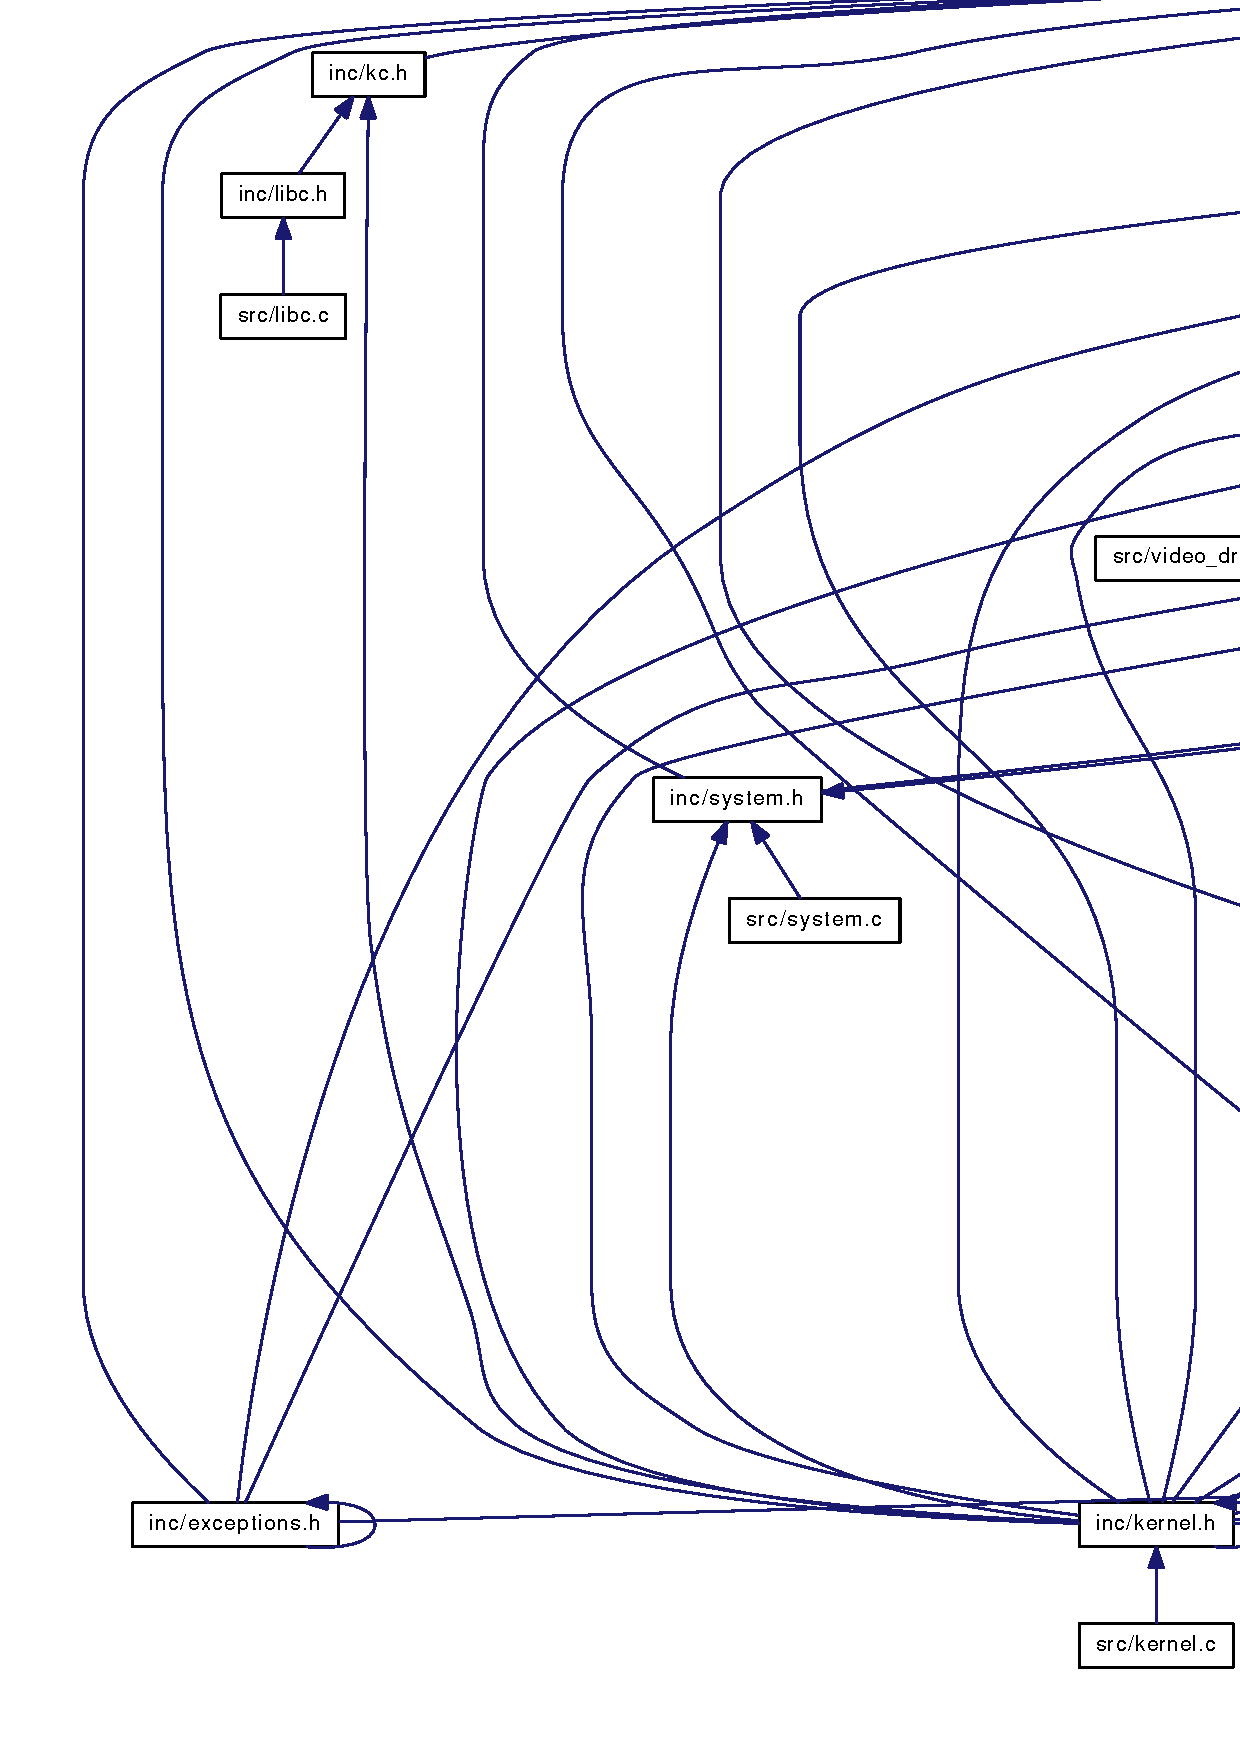
\includegraphics[width=420pt]{defs_8h__dep__incl}
\end{center}
\end{figure}
\subsection*{Defines}
\begin{DoxyCompactItemize}
\item 
\#define \hyperlink{defs_8h_a71809484a26cd96c6abe839a0a8a289d}{byte}~unsigned char
\begin{DoxyCompactList}\small\item\em DefineBrief. \item\end{DoxyCompactList}\item 
\#define \hyperlink{defs_8h_a836535f59bf515522a395858a8029d42}{word}~short int
\begin{DoxyCompactList}\small\item\em DefineBrief. \item\end{DoxyCompactList}\item 
\#define \hyperlink{defs_8h_a55849dc98f28432a4601c29a4a352a97}{dword}~int
\begin{DoxyCompactList}\small\item\em DefineBrief. \item\end{DoxyCompactList}\item 
\#define \hyperlink{defs_8h_aa8cecfc5c5c054d2875c03e77b7be15d}{TRUE}~1
\begin{DoxyCompactList}\small\item\em DefineBrief. \item\end{DoxyCompactList}\item 
\#define \hyperlink{defs_8h_aa93f0eb578d23995850d61f7d61c55c1}{FALSE}~!TRUE
\begin{DoxyCompactList}\small\item\em DefineBrief. \item\end{DoxyCompactList}\item 
\#define \hyperlink{defs_8h_aba51915c87d64af47fb1cc59348961c9}{OK}~TRUE
\begin{DoxyCompactList}\small\item\em DefineBrief. \item\end{DoxyCompactList}\item 
\#define \hyperlink{defs_8h_a8fe83ac76edc595f6b98cd4a4127aed5}{ERROR}~FALSE
\begin{DoxyCompactList}\small\item\em DefineBrief. \item\end{DoxyCompactList}\item 
\#define \hyperlink{defs_8h_a8026e8d87908b0239264d643c90183f5}{\_\-READ}~0x01
\begin{DoxyCompactList}\small\item\em DefineBrief. \item\end{DoxyCompactList}\item 
\#define \hyperlink{defs_8h_a622e22a8bb12b59a4e14802f6aa1737e}{\_\-WRITE}~0x02
\begin{DoxyCompactList}\small\item\em DefineBrief. \item\end{DoxyCompactList}\item 
\#define \hyperlink{defs_8h_ad930a240d62012e99d9f9dc2b618b3e8}{SEND\_\-TO\_\-VIDEO}~1
\begin{DoxyCompactList}\small\item\em DefineBrief. \item\end{DoxyCompactList}\item 
\#define \hyperlink{defs_8h_ae30b01f0637fa2a2ef0ee72fbbaee2a2}{WRITE\_\-ON\_\-TTY}~0
\begin{DoxyCompactList}\small\item\em DefineBrief. \item\end{DoxyCompactList}\item 
\#define \hyperlink{defs_8h_a057b722e3d1168cf748c4936f59b7769}{TTY\_\-RAW}~0
\begin{DoxyCompactList}\small\item\em DefineBrief. \item\end{DoxyCompactList}\item 
\#define \hyperlink{defs_8h_afd70646efe5984e361c17010322a5711}{TTY\_\-CANONICAL}~1
\begin{DoxyCompactList}\small\item\em DefineBrief. \item\end{DoxyCompactList}\item 
\#define \hyperlink{defs_8h_a0b674752cca6d434a1a69f40877eb2be}{LOAD}~0
\begin{DoxyCompactList}\small\item\em DefineBrief. \item\end{DoxyCompactList}\item 
\#define \hyperlink{defs_8h_ab2868d85c8a74e3ee08bdc44580e2235}{SAVE}~1
\begin{DoxyCompactList}\small\item\em DefineBrief. \item\end{DoxyCompactList}\item 
\#define \hyperlink{defs_8h_ac00bfb46347d26fdc58568fe1ab5fa5b}{STDIN}~0
\begin{DoxyCompactList}\small\item\em DefineBrief. \item\end{DoxyCompactList}\item 
\#define \hyperlink{defs_8h_a8875037d0772a4fc34516f1e03d7e238}{STDOUT}~1
\begin{DoxyCompactList}\small\item\em DefineBrief. \item\end{DoxyCompactList}\item 
\#define \hyperlink{defs_8h_ac242dc8b10d052be6043664a044fdb87}{IN\_\-ATT}~2
\begin{DoxyCompactList}\small\item\em DefineBrief. \item\end{DoxyCompactList}\item 
\#define \hyperlink{defs_8h_a26743ec6d52be788fe60acfe2865d5ae}{OUT\_\-ATT}~3
\begin{DoxyCompactList}\small\item\em DefineBrief. \item\end{DoxyCompactList}\item 
\#define \hyperlink{defs_8h_a7ae1ae649327b67ce210e47ea1ed07dc}{ATOMIC}~1
\begin{DoxyCompactList}\small\item\em DefineBrief. \item\end{DoxyCompactList}\item 
\#define \hyperlink{defs_8h_a33d80cf420a3739faa00760673eee7db}{UNATOMIC}~!ATOMIC
\begin{DoxyCompactList}\small\item\em DefineBrief. \item\end{DoxyCompactList}\item 
\#define \hyperlink{defs_8h_a2a375179c125d0867430c6778c343b6f}{FOREGROUND}~0
\begin{DoxyCompactList}\small\item\em DefineBrief. \item\end{DoxyCompactList}\item 
\#define \hyperlink{defs_8h_a850b2f07a67b73890889e63fb8a49fda}{BACKGROUND}~1
\begin{DoxyCompactList}\small\item\em DefineBrief. \item\end{DoxyCompactList}\item 
\#define \hyperlink{defs_8h_a1841fd1a462d245d8c73dce55e2f45da}{KB}~$\ast$ (1 $<$$<$ 10)
\begin{DoxyCompactList}\small\item\em DefineBrief. \item\end{DoxyCompactList}\item 
\#define \hyperlink{defs_8h_aa6b38d492364d98453284934ed7caee9}{MB}~$\ast$ (1 $<$$<$ 20)
\begin{DoxyCompactList}\small\item\em DefineBrief. \item\end{DoxyCompactList}\item 
\#define \hyperlink{defs_8h_a94ad616f6fdced1466e60a7add259f3c}{KERNEL\_\-SPACE}~0x00000000
\begin{DoxyCompactList}\small\item\em DefineBrief. \item\end{DoxyCompactList}\item 
\#define \hyperlink{defs_8h_a2d85dcc33ff0b653b17210b6861b9030}{KERNEL\_\-SPACE\_\-SIZE}~(8 MB)
\begin{DoxyCompactList}\small\item\em DefineBrief. \item\end{DoxyCompactList}\item 
\#define \hyperlink{defs_8h_aecbd22e428b6301e4e4c34e96af47b19}{MALLOC\_\-SPACE}~(KERNEL\_\-SPACE + KERNEL\_\-SPACE\_\-SIZE)
\begin{DoxyCompactList}\small\item\em DefineBrief. \item\end{DoxyCompactList}\item 
\#define \hyperlink{defs_8h_a15861042d55ace11a79fe0b3da5814e8}{MALLOC\_\-SPACE\_\-SIZE}~(8 MB)
\begin{DoxyCompactList}\small\item\em DefineBrief. \item\end{DoxyCompactList}\item 
\#define \hyperlink{defs_8h_a1ec9bed1a229be7be1c30b971ac19148}{TOTAL\_\-MEMORY\_\-SIZE}~(KERNEL\_\-SPACE\_\-SIZE + MALLOC\_\-SPACE\_\-SIZE)
\begin{DoxyCompactList}\small\item\em DefineBrief. \item\end{DoxyCompactList}\item 
\#define \hyperlink{defs_8h_a7d467c1d283fdfa1f2081ba1e0d01b6e}{PAGE\_\-SIZE}~(4 KB)
\begin{DoxyCompactList}\small\item\em DefineBrief. \item\end{DoxyCompactList}\item 
\#define \hyperlink{defs_8h_afdb5118f31e3b405e768aae86185858f}{PAGE\_\-ENTRY\_\-SIZE}~sizeof(unsigned int)
\begin{DoxyCompactList}\small\item\em DefineBrief. \item\end{DoxyCompactList}\item 
\#define \hyperlink{defs_8h_a8e5feaae0050abc2f048607651293efe}{PAGE\_\-ENTRIES\_\-PER\_\-TABLE}~(PAGE\_\-SIZE / PAGE\_\-ENTRY\_\-SIZE)
\begin{DoxyCompactList}\small\item\em DefineBrief. \item\end{DoxyCompactList}\item 
\#define \hyperlink{defs_8h_a23bbe65918fee446b09dc6d3f92e0bac}{KERNEL\_\-TABLES\_\-QTY}~(KERNEL\_\-SPACE\_\-SIZE / (PAGE\_\-SIZE $\ast$ PAGE\_\-ENTRIES\_\-PER\_\-TABLE))
\begin{DoxyCompactList}\small\item\em DefineBrief. \item\end{DoxyCompactList}\item 
\#define \hyperlink{defs_8h_a6f5a06effdbd61bd2873b52fd019ac2d}{MALLOC\_\-TABLES\_\-QTY}~(MALLOC\_\-SPACE\_\-SIZE / (PAGE\_\-SIZE $\ast$ PAGE\_\-ENTRIES\_\-PER\_\-TABLE))
\begin{DoxyCompactList}\small\item\em DefineBrief. \item\end{DoxyCompactList}\item 
\#define \hyperlink{defs_8h_a2fe5b1c83a789cd19496b550290a10e2}{PAGE\_\-TABLES\_\-QTY}~(KERNEL\_\-TABLES\_\-QTY + MALLOC\_\-TABLES\_\-QTY)
\begin{DoxyCompactList}\small\item\em DefineBrief. \item\end{DoxyCompactList}\item 
\#define \hyperlink{defs_8h_a20851f5fd859765b86e8b9fc8b30572e}{FRAMES\_\-PER\_\-TABLE}~(PAGE\_\-ENTRIES\_\-PER\_\-TABLE / PAGES\_\-PER\_\-FRAME)
\begin{DoxyCompactList}\small\item\em DefineBrief. \item\end{DoxyCompactList}\item 
\#define \hyperlink{defs_8h_a7f80e4b553d435a097d07c74652ee861}{TOTAL\_\-FRAMES\_\-QTY}~(MALLOC\_\-TABLES\_\-QTY $\ast$ FRAMES\_\-PER\_\-TABLE)
\begin{DoxyCompactList}\small\item\em DefineBrief. \item\end{DoxyCompactList}\item 
\#define \hyperlink{defs_8h_a2cac3b477c52f9e0329f6b6d8050aa34}{FIRST\_\-KERNEL\_\-TABLE}~0
\begin{DoxyCompactList}\small\item\em DefineBrief. \item\end{DoxyCompactList}\item 
\#define \hyperlink{defs_8h_a8d40ab04e10902bcdca98d83ad7b5155}{FIRST\_\-MALLOC\_\-TABLE}~FIRST\_\-KERNEL\_\-TABLE + KERNEL\_\-TABLES\_\-QTY
\begin{DoxyCompactList}\small\item\em DefineBrief. \item\end{DoxyCompactList}\item 
\#define \hyperlink{defs_8h_ab84f195ddb9b6b192088157ecf8c835f}{PAGES\_\-PER\_\-INT}~((int)(sizeof(unsigned int)) $\ast$ 8)
\begin{DoxyCompactList}\small\item\em DefineBrief. \item\end{DoxyCompactList}\item 
\#define \hyperlink{defs_8h_a2d4f316ac84e27da715d76af7694e4f9}{INTS\_\-PER\_\-TABLE}~(PAGE\_\-ENTRIES\_\-PER\_\-TABLE / 32)
\begin{DoxyCompactList}\small\item\em DefineBrief. \item\end{DoxyCompactList}\item 
\#define \hyperlink{defs_8h_aa5efd9de5f0408f54365716967adbb87}{BITMAP\_\-SIZE}~(INTS\_\-PER\_\-TABLE $\ast$ MALLOC\_\-TABLES\_\-QTY)
\begin{DoxyCompactList}\small\item\em DefineBrief. \item\end{DoxyCompactList}\item 
\#define \hyperlink{defs_8h_aa810745c50d2723a02ccb8059f7e11b6}{MAX\_\-MAPPED\_\-ADDRESS}~(TOTAL\_\-MEMORY\_\-SIZE -\/ 1)
\begin{DoxyCompactList}\small\item\em DefineBrief. \item\end{DoxyCompactList}\item 
\#define \hyperlink{defs_8h_ac64bf9bd32b5cab356a11a0259ea9fb6}{getBitmapIndex}(addr)~(((addr) / (unsigned)PAGE\_\-SIZE) / (unsigned)PAGES\_\-PER\_\-INT)
\begin{DoxyCompactList}\small\item\em DefineBrief. \item\end{DoxyCompactList}\item 
\#define \hyperlink{defs_8h_aeab9875301d2688f746797e91126b16f}{getBitmapOffset}(addr)~(0x00000001 $<$$<$ (((addr) / PAGE\_\-SIZE) \% PAGES\_\-PER\_\-INT))
\begin{DoxyCompactList}\small\item\em DefineBrief. \item\end{DoxyCompactList}\item 
\#define \hyperlink{defs_8h_a9d6fc23740ab9f37272a3299949d3c11}{OFFSET\_\-MASK}~0xFFFFF000
\begin{DoxyCompactList}\small\item\em DefineBrief. \item\end{DoxyCompactList}\item 
\#define \hyperlink{defs_8h_ae60b3b1ff706b666b7eaef0a715c4490}{ACS\_\-PRESENT}~0x80
\begin{DoxyCompactList}\small\item\em DefineBrief. \item\end{DoxyCompactList}\item 
\#define \hyperlink{defs_8h_a0efe10800f018eacf8c3f55e7b37647e}{ACS\_\-CSEG}~0x18
\begin{DoxyCompactList}\small\item\em DefineBrief. \item\end{DoxyCompactList}\item 
\#define \hyperlink{defs_8h_a8e220a1ec7efd60bb8e56d73f480825c}{ACS\_\-DSEG}~0x10
\begin{DoxyCompactList}\small\item\em DefineBrief. \item\end{DoxyCompactList}\item 
\#define \hyperlink{defs_8h_a2ed04c0e682556517761ecb25b15fe12}{ACS\_\-READ}~0x02
\begin{DoxyCompactList}\small\item\em DefineBrief. \item\end{DoxyCompactList}\item 
\#define \hyperlink{defs_8h_a409bddc73ed57ee81de6ca917cea2b27}{ACS\_\-WRITE}~0x02
\begin{DoxyCompactList}\small\item\em DefineBrief. \item\end{DoxyCompactList}\item 
\#define \hyperlink{defs_8h_a7a7ce494703b76e2a80a3e820be0fd49}{ACS\_\-IDT}~ACS\_\-DSEG
\begin{DoxyCompactList}\small\item\em DefineBrief. \item\end{DoxyCompactList}\item 
\#define \hyperlink{defs_8h_aab317390db9c07d896f467b7e2314698}{ACS\_\-INT\_\-386}~0x0E
\begin{DoxyCompactList}\small\item\em DefineBrief. \item\end{DoxyCompactList}\item 
\#define \hyperlink{defs_8h_a8cc2a7c8288db5cf7281a58f92bc1f17}{ACS\_\-INT}~( ACS\_\-PRESENT $|$ ACS\_\-INT\_\-386 )
\begin{DoxyCompactList}\small\item\em DefineBrief. \item\end{DoxyCompactList}\item 
\#define \hyperlink{defs_8h_aa7ddb691bab273f0807425fe80040f1d}{ACS\_\-CODE}~(ACS\_\-PRESENT $|$ ACS\_\-CSEG $|$ ACS\_\-READ)
\begin{DoxyCompactList}\small\item\em DefineBrief. \item\end{DoxyCompactList}\item 
\#define \hyperlink{defs_8h_ac1572e04dde6fdf2710a883fff94cab4}{ACS\_\-DATA}~(ACS\_\-PRESENT $|$ ACS\_\-DSEG $|$ ACS\_\-WRITE)
\begin{DoxyCompactList}\small\item\em DefineBrief. \item\end{DoxyCompactList}\item 
\#define \hyperlink{defs_8h_a2f319798ef0f9dd5926f95d90697b7ab}{ACS\_\-STACK}~(ACS\_\-PRESENT $|$ ACS\_\-DSEG $|$ ACS\_\-WRITE)
\begin{DoxyCompactList}\small\item\em DefineBrief. \item\end{DoxyCompactList}\item 
\#define \hyperlink{defs_8h_a070d2ce7b6bb7e5c05602aa8c308d0c4}{NULL}~(void $\ast$)0x0
\begin{DoxyCompactList}\small\item\em NULL pointer definition. \item\end{DoxyCompactList}\end{DoxyCompactItemize}


\subsection{Detailed Description}
OS inner defines. \begin{DoxyAuthor}{Author}
Luciano Zemin, Nicolás Magni, Nicolás Purita 
\end{DoxyAuthor}


Definition in file \hyperlink{defs_8h_source}{defs.h}.



\subsection{Define Documentation}
\hypertarget{defs_8h_a8026e8d87908b0239264d643c90183f5}{
\index{defs.h@{defs.h}!\_\-READ@{\_\-READ}}
\index{\_\-READ@{\_\-READ}!defs.h@{defs.h}}
\subsubsection[{\_\-READ}]{\setlength{\rightskip}{0pt plus 5cm}\#define \_\-READ~0x01}}
\label{defs_8h_a8026e8d87908b0239264d643c90183f5}


DefineBrief. 



Definition at line 53 of file defs.h.

\hypertarget{defs_8h_a622e22a8bb12b59a4e14802f6aa1737e}{
\index{defs.h@{defs.h}!\_\-WRITE@{\_\-WRITE}}
\index{\_\-WRITE@{\_\-WRITE}!defs.h@{defs.h}}
\subsubsection[{\_\-WRITE}]{\setlength{\rightskip}{0pt plus 5cm}\#define \_\-WRITE~0x02}}
\label{defs_8h_a622e22a8bb12b59a4e14802f6aa1737e}


DefineBrief. 



Definition at line 58 of file defs.h.

\hypertarget{defs_8h_aa7ddb691bab273f0807425fe80040f1d}{
\index{defs.h@{defs.h}!ACS\_\-CODE@{ACS\_\-CODE}}
\index{ACS\_\-CODE@{ACS\_\-CODE}!defs.h@{defs.h}}
\subsubsection[{ACS\_\-CODE}]{\setlength{\rightskip}{0pt plus 5cm}\#define ACS\_\-CODE~(ACS\_\-PRESENT $|$ ACS\_\-CSEG $|$ ACS\_\-READ)}}
\label{defs_8h_aa7ddb691bab273f0807425fe80040f1d}


DefineBrief. 



Definition at line 313 of file defs.h.

\hypertarget{defs_8h_a0efe10800f018eacf8c3f55e7b37647e}{
\index{defs.h@{defs.h}!ACS\_\-CSEG@{ACS\_\-CSEG}}
\index{ACS\_\-CSEG@{ACS\_\-CSEG}!defs.h@{defs.h}}
\subsubsection[{ACS\_\-CSEG}]{\setlength{\rightskip}{0pt plus 5cm}\#define ACS\_\-CSEG~0x18}}
\label{defs_8h_a0efe10800f018eacf8c3f55e7b37647e}


DefineBrief. 



Definition at line 277 of file defs.h.

\hypertarget{defs_8h_ac1572e04dde6fdf2710a883fff94cab4}{
\index{defs.h@{defs.h}!ACS\_\-DATA@{ACS\_\-DATA}}
\index{ACS\_\-DATA@{ACS\_\-DATA}!defs.h@{defs.h}}
\subsubsection[{ACS\_\-DATA}]{\setlength{\rightskip}{0pt plus 5cm}\#define ACS\_\-DATA~(ACS\_\-PRESENT $|$ ACS\_\-DSEG $|$ ACS\_\-WRITE)}}
\label{defs_8h_ac1572e04dde6fdf2710a883fff94cab4}


DefineBrief. 



Definition at line 318 of file defs.h.

\hypertarget{defs_8h_a8e220a1ec7efd60bb8e56d73f480825c}{
\index{defs.h@{defs.h}!ACS\_\-DSEG@{ACS\_\-DSEG}}
\index{ACS\_\-DSEG@{ACS\_\-DSEG}!defs.h@{defs.h}}
\subsubsection[{ACS\_\-DSEG}]{\setlength{\rightskip}{0pt plus 5cm}\#define ACS\_\-DSEG~0x10}}
\label{defs_8h_a8e220a1ec7efd60bb8e56d73f480825c}


DefineBrief. 



Definition at line 282 of file defs.h.

\hypertarget{defs_8h_a7a7ce494703b76e2a80a3e820be0fd49}{
\index{defs.h@{defs.h}!ACS\_\-IDT@{ACS\_\-IDT}}
\index{ACS\_\-IDT@{ACS\_\-IDT}!defs.h@{defs.h}}
\subsubsection[{ACS\_\-IDT}]{\setlength{\rightskip}{0pt plus 5cm}\#define ACS\_\-IDT~ACS\_\-DSEG}}
\label{defs_8h_a7a7ce494703b76e2a80a3e820be0fd49}


DefineBrief. 



Definition at line 297 of file defs.h.

\hypertarget{defs_8h_a8cc2a7c8288db5cf7281a58f92bc1f17}{
\index{defs.h@{defs.h}!ACS\_\-INT@{ACS\_\-INT}}
\index{ACS\_\-INT@{ACS\_\-INT}!defs.h@{defs.h}}
\subsubsection[{ACS\_\-INT}]{\setlength{\rightskip}{0pt plus 5cm}\#define ACS\_\-INT~( ACS\_\-PRESENT $|$ ACS\_\-INT\_\-386 )}}
\label{defs_8h_a8cc2a7c8288db5cf7281a58f92bc1f17}


DefineBrief. 



Definition at line 307 of file defs.h.

\hypertarget{defs_8h_aab317390db9c07d896f467b7e2314698}{
\index{defs.h@{defs.h}!ACS\_\-INT\_\-386@{ACS\_\-INT\_\-386}}
\index{ACS\_\-INT\_\-386@{ACS\_\-INT\_\-386}!defs.h@{defs.h}}
\subsubsection[{ACS\_\-INT\_\-386}]{\setlength{\rightskip}{0pt plus 5cm}\#define ACS\_\-INT\_\-386~0x0E}}
\label{defs_8h_aab317390db9c07d896f467b7e2314698}


DefineBrief. 



Definition at line 302 of file defs.h.

\hypertarget{defs_8h_ae60b3b1ff706b666b7eaef0a715c4490}{
\index{defs.h@{defs.h}!ACS\_\-PRESENT@{ACS\_\-PRESENT}}
\index{ACS\_\-PRESENT@{ACS\_\-PRESENT}!defs.h@{defs.h}}
\subsubsection[{ACS\_\-PRESENT}]{\setlength{\rightskip}{0pt plus 5cm}\#define ACS\_\-PRESENT~0x80}}
\label{defs_8h_ae60b3b1ff706b666b7eaef0a715c4490}


DefineBrief. 



Definition at line 272 of file defs.h.

\hypertarget{defs_8h_a2ed04c0e682556517761ecb25b15fe12}{
\index{defs.h@{defs.h}!ACS\_\-READ@{ACS\_\-READ}}
\index{ACS\_\-READ@{ACS\_\-READ}!defs.h@{defs.h}}
\subsubsection[{ACS\_\-READ}]{\setlength{\rightskip}{0pt plus 5cm}\#define ACS\_\-READ~0x02}}
\label{defs_8h_a2ed04c0e682556517761ecb25b15fe12}


DefineBrief. 



Definition at line 287 of file defs.h.

\hypertarget{defs_8h_a2f319798ef0f9dd5926f95d90697b7ab}{
\index{defs.h@{defs.h}!ACS\_\-STACK@{ACS\_\-STACK}}
\index{ACS\_\-STACK@{ACS\_\-STACK}!defs.h@{defs.h}}
\subsubsection[{ACS\_\-STACK}]{\setlength{\rightskip}{0pt plus 5cm}\#define ACS\_\-STACK~(ACS\_\-PRESENT $|$ ACS\_\-DSEG $|$ ACS\_\-WRITE)}}
\label{defs_8h_a2f319798ef0f9dd5926f95d90697b7ab}


DefineBrief. 



Definition at line 323 of file defs.h.

\hypertarget{defs_8h_a409bddc73ed57ee81de6ca917cea2b27}{
\index{defs.h@{defs.h}!ACS\_\-WRITE@{ACS\_\-WRITE}}
\index{ACS\_\-WRITE@{ACS\_\-WRITE}!defs.h@{defs.h}}
\subsubsection[{ACS\_\-WRITE}]{\setlength{\rightskip}{0pt plus 5cm}\#define ACS\_\-WRITE~0x02}}
\label{defs_8h_a409bddc73ed57ee81de6ca917cea2b27}


DefineBrief. 



Definition at line 292 of file defs.h.

\hypertarget{defs_8h_a7ae1ae649327b67ce210e47ea1ed07dc}{
\index{defs.h@{defs.h}!ATOMIC@{ATOMIC}}
\index{ATOMIC@{ATOMIC}!defs.h@{defs.h}}
\subsubsection[{ATOMIC}]{\setlength{\rightskip}{0pt plus 5cm}\#define ATOMIC~1}}
\label{defs_8h_a7ae1ae649327b67ce210e47ea1ed07dc}


DefineBrief. 



Definition at line 118 of file defs.h.

\hypertarget{defs_8h_a850b2f07a67b73890889e63fb8a49fda}{
\index{defs.h@{defs.h}!BACKGROUND@{BACKGROUND}}
\index{BACKGROUND@{BACKGROUND}!defs.h@{defs.h}}
\subsubsection[{BACKGROUND}]{\setlength{\rightskip}{0pt plus 5cm}\#define BACKGROUND~1}}
\label{defs_8h_a850b2f07a67b73890889e63fb8a49fda}


DefineBrief. 



Definition at line 133 of file defs.h.

\hypertarget{defs_8h_aa5efd9de5f0408f54365716967adbb87}{
\index{defs.h@{defs.h}!BITMAP\_\-SIZE@{BITMAP\_\-SIZE}}
\index{BITMAP\_\-SIZE@{BITMAP\_\-SIZE}!defs.h@{defs.h}}
\subsubsection[{BITMAP\_\-SIZE}]{\setlength{\rightskip}{0pt plus 5cm}\#define BITMAP\_\-SIZE~(INTS\_\-PER\_\-TABLE $\ast$ MALLOC\_\-TABLES\_\-QTY)}}
\label{defs_8h_aa5efd9de5f0408f54365716967adbb87}


DefineBrief. 



Definition at line 245 of file defs.h.

\hypertarget{defs_8h_a71809484a26cd96c6abe839a0a8a289d}{
\index{defs.h@{defs.h}!byte@{byte}}
\index{byte@{byte}!defs.h@{defs.h}}
\subsubsection[{byte}]{\setlength{\rightskip}{0pt plus 5cm}\#define byte~unsigned char}}
\label{defs_8h_a71809484a26cd96c6abe839a0a8a289d}


DefineBrief. 



Definition at line 17 of file defs.h.

\hypertarget{defs_8h_a55849dc98f28432a4601c29a4a352a97}{
\index{defs.h@{defs.h}!dword@{dword}}
\index{dword@{dword}!defs.h@{defs.h}}
\subsubsection[{dword}]{\setlength{\rightskip}{0pt plus 5cm}\#define dword~int}}
\label{defs_8h_a55849dc98f28432a4601c29a4a352a97}


DefineBrief. 



Definition at line 27 of file defs.h.

\hypertarget{defs_8h_a8fe83ac76edc595f6b98cd4a4127aed5}{
\index{defs.h@{defs.h}!ERROR@{ERROR}}
\index{ERROR@{ERROR}!defs.h@{defs.h}}
\subsubsection[{ERROR}]{\setlength{\rightskip}{0pt plus 5cm}\#define ERROR~FALSE}}
\label{defs_8h_a8fe83ac76edc595f6b98cd4a4127aed5}


DefineBrief. 



Definition at line 47 of file defs.h.

\hypertarget{defs_8h_aa93f0eb578d23995850d61f7d61c55c1}{
\index{defs.h@{defs.h}!FALSE@{FALSE}}
\index{FALSE@{FALSE}!defs.h@{defs.h}}
\subsubsection[{FALSE}]{\setlength{\rightskip}{0pt plus 5cm}\#define FALSE~!TRUE}}
\label{defs_8h_aa93f0eb578d23995850d61f7d61c55c1}


DefineBrief. 



Definition at line 37 of file defs.h.

\hypertarget{defs_8h_a2cac3b477c52f9e0329f6b6d8050aa34}{
\index{defs.h@{defs.h}!FIRST\_\-KERNEL\_\-TABLE@{FIRST\_\-KERNEL\_\-TABLE}}
\index{FIRST\_\-KERNEL\_\-TABLE@{FIRST\_\-KERNEL\_\-TABLE}!defs.h@{defs.h}}
\subsubsection[{FIRST\_\-KERNEL\_\-TABLE}]{\setlength{\rightskip}{0pt plus 5cm}\#define FIRST\_\-KERNEL\_\-TABLE~0}}
\label{defs_8h_a2cac3b477c52f9e0329f6b6d8050aa34}


DefineBrief. 



Definition at line 223 of file defs.h.

\hypertarget{defs_8h_a8d40ab04e10902bcdca98d83ad7b5155}{
\index{defs.h@{defs.h}!FIRST\_\-MALLOC\_\-TABLE@{FIRST\_\-MALLOC\_\-TABLE}}
\index{FIRST\_\-MALLOC\_\-TABLE@{FIRST\_\-MALLOC\_\-TABLE}!defs.h@{defs.h}}
\subsubsection[{FIRST\_\-MALLOC\_\-TABLE}]{\setlength{\rightskip}{0pt plus 5cm}\#define FIRST\_\-MALLOC\_\-TABLE~FIRST\_\-KERNEL\_\-TABLE + KERNEL\_\-TABLES\_\-QTY}}
\label{defs_8h_a8d40ab04e10902bcdca98d83ad7b5155}


DefineBrief. 



Definition at line 228 of file defs.h.

\hypertarget{defs_8h_a2a375179c125d0867430c6778c343b6f}{
\index{defs.h@{defs.h}!FOREGROUND@{FOREGROUND}}
\index{FOREGROUND@{FOREGROUND}!defs.h@{defs.h}}
\subsubsection[{FOREGROUND}]{\setlength{\rightskip}{0pt plus 5cm}\#define FOREGROUND~0}}
\label{defs_8h_a2a375179c125d0867430c6778c343b6f}


DefineBrief. 



Definition at line 128 of file defs.h.

\hypertarget{defs_8h_a20851f5fd859765b86e8b9fc8b30572e}{
\index{defs.h@{defs.h}!FRAMES\_\-PER\_\-TABLE@{FRAMES\_\-PER\_\-TABLE}}
\index{FRAMES\_\-PER\_\-TABLE@{FRAMES\_\-PER\_\-TABLE}!defs.h@{defs.h}}
\subsubsection[{FRAMES\_\-PER\_\-TABLE}]{\setlength{\rightskip}{0pt plus 5cm}\#define FRAMES\_\-PER\_\-TABLE~(PAGE\_\-ENTRIES\_\-PER\_\-TABLE / PAGES\_\-PER\_\-FRAME)}}
\label{defs_8h_a20851f5fd859765b86e8b9fc8b30572e}


DefineBrief. 



Definition at line 211 of file defs.h.

\hypertarget{defs_8h_ac64bf9bd32b5cab356a11a0259ea9fb6}{
\index{defs.h@{defs.h}!getBitmapIndex@{getBitmapIndex}}
\index{getBitmapIndex@{getBitmapIndex}!defs.h@{defs.h}}
\subsubsection[{getBitmapIndex}]{\setlength{\rightskip}{0pt plus 5cm}\#define getBitmapIndex(addr)~(((addr) / (unsigned)PAGE\_\-SIZE) / (unsigned)PAGES\_\-PER\_\-INT)}}
\label{defs_8h_ac64bf9bd32b5cab356a11a0259ea9fb6}


DefineBrief. 



Definition at line 255 of file defs.h.

\hypertarget{defs_8h_aeab9875301d2688f746797e91126b16f}{
\index{defs.h@{defs.h}!getBitmapOffset@{getBitmapOffset}}
\index{getBitmapOffset@{getBitmapOffset}!defs.h@{defs.h}}
\subsubsection[{getBitmapOffset}]{\setlength{\rightskip}{0pt plus 5cm}\#define getBitmapOffset(addr)~(0x00000001 $<$$<$ (((addr) / PAGE\_\-SIZE) \% PAGES\_\-PER\_\-INT))}}
\label{defs_8h_aeab9875301d2688f746797e91126b16f}


DefineBrief. 



Definition at line 260 of file defs.h.

\hypertarget{defs_8h_ac242dc8b10d052be6043664a044fdb87}{
\index{defs.h@{defs.h}!IN\_\-ATT@{IN\_\-ATT}}
\index{IN\_\-ATT@{IN\_\-ATT}!defs.h@{defs.h}}
\subsubsection[{IN\_\-ATT}]{\setlength{\rightskip}{0pt plus 5cm}\#define IN\_\-ATT~2}}
\label{defs_8h_ac242dc8b10d052be6043664a044fdb87}


DefineBrief. 



Definition at line 107 of file defs.h.

\hypertarget{defs_8h_a2d4f316ac84e27da715d76af7694e4f9}{
\index{defs.h@{defs.h}!INTS\_\-PER\_\-TABLE@{INTS\_\-PER\_\-TABLE}}
\index{INTS\_\-PER\_\-TABLE@{INTS\_\-PER\_\-TABLE}!defs.h@{defs.h}}
\subsubsection[{INTS\_\-PER\_\-TABLE}]{\setlength{\rightskip}{0pt plus 5cm}\#define INTS\_\-PER\_\-TABLE~(PAGE\_\-ENTRIES\_\-PER\_\-TABLE / 32)}}
\label{defs_8h_a2d4f316ac84e27da715d76af7694e4f9}


DefineBrief. 



Definition at line 240 of file defs.h.

\hypertarget{defs_8h_a1841fd1a462d245d8c73dce55e2f45da}{
\index{defs.h@{defs.h}!KB@{KB}}
\index{KB@{KB}!defs.h@{defs.h}}
\subsubsection[{KB}]{\setlength{\rightskip}{0pt plus 5cm}\#define KB~$\ast$ (1 $<$$<$ 10)}}
\label{defs_8h_a1841fd1a462d245d8c73dce55e2f45da}


DefineBrief. 



Definition at line 140 of file defs.h.

\hypertarget{defs_8h_a94ad616f6fdced1466e60a7add259f3c}{
\index{defs.h@{defs.h}!KERNEL\_\-SPACE@{KERNEL\_\-SPACE}}
\index{KERNEL\_\-SPACE@{KERNEL\_\-SPACE}!defs.h@{defs.h}}
\subsubsection[{KERNEL\_\-SPACE}]{\setlength{\rightskip}{0pt plus 5cm}\#define KERNEL\_\-SPACE~0x00000000}}
\label{defs_8h_a94ad616f6fdced1466e60a7add259f3c}


DefineBrief. 



Definition at line 152 of file defs.h.

\hypertarget{defs_8h_a2d85dcc33ff0b653b17210b6861b9030}{
\index{defs.h@{defs.h}!KERNEL\_\-SPACE\_\-SIZE@{KERNEL\_\-SPACE\_\-SIZE}}
\index{KERNEL\_\-SPACE\_\-SIZE@{KERNEL\_\-SPACE\_\-SIZE}!defs.h@{defs.h}}
\subsubsection[{KERNEL\_\-SPACE\_\-SIZE}]{\setlength{\rightskip}{0pt plus 5cm}\#define KERNEL\_\-SPACE\_\-SIZE~(8 MB)}}
\label{defs_8h_a2d85dcc33ff0b653b17210b6861b9030}


DefineBrief. 



Definition at line 157 of file defs.h.

\hypertarget{defs_8h_a23bbe65918fee446b09dc6d3f92e0bac}{
\index{defs.h@{defs.h}!KERNEL\_\-TABLES\_\-QTY@{KERNEL\_\-TABLES\_\-QTY}}
\index{KERNEL\_\-TABLES\_\-QTY@{KERNEL\_\-TABLES\_\-QTY}!defs.h@{defs.h}}
\subsubsection[{KERNEL\_\-TABLES\_\-QTY}]{\setlength{\rightskip}{0pt plus 5cm}\#define KERNEL\_\-TABLES\_\-QTY~(KERNEL\_\-SPACE\_\-SIZE / (PAGE\_\-SIZE $\ast$ PAGE\_\-ENTRIES\_\-PER\_\-TABLE))}}
\label{defs_8h_a23bbe65918fee446b09dc6d3f92e0bac}


DefineBrief. 



Definition at line 194 of file defs.h.

\hypertarget{defs_8h_a0b674752cca6d434a1a69f40877eb2be}{
\index{defs.h@{defs.h}!LOAD@{LOAD}}
\index{LOAD@{LOAD}!defs.h@{defs.h}}
\subsubsection[{LOAD}]{\setlength{\rightskip}{0pt plus 5cm}\#define LOAD~0}}
\label{defs_8h_a0b674752cca6d434a1a69f40877eb2be}


DefineBrief. 



Definition at line 86 of file defs.h.

\hypertarget{defs_8h_aecbd22e428b6301e4e4c34e96af47b19}{
\index{defs.h@{defs.h}!MALLOC\_\-SPACE@{MALLOC\_\-SPACE}}
\index{MALLOC\_\-SPACE@{MALLOC\_\-SPACE}!defs.h@{defs.h}}
\subsubsection[{MALLOC\_\-SPACE}]{\setlength{\rightskip}{0pt plus 5cm}\#define MALLOC\_\-SPACE~(KERNEL\_\-SPACE + KERNEL\_\-SPACE\_\-SIZE)}}
\label{defs_8h_aecbd22e428b6301e4e4c34e96af47b19}


DefineBrief. 



Definition at line 162 of file defs.h.

\hypertarget{defs_8h_a15861042d55ace11a79fe0b3da5814e8}{
\index{defs.h@{defs.h}!MALLOC\_\-SPACE\_\-SIZE@{MALLOC\_\-SPACE\_\-SIZE}}
\index{MALLOC\_\-SPACE\_\-SIZE@{MALLOC\_\-SPACE\_\-SIZE}!defs.h@{defs.h}}
\subsubsection[{MALLOC\_\-SPACE\_\-SIZE}]{\setlength{\rightskip}{0pt plus 5cm}\#define MALLOC\_\-SPACE\_\-SIZE~(8 MB)}}
\label{defs_8h_a15861042d55ace11a79fe0b3da5814e8}


DefineBrief. 



Definition at line 167 of file defs.h.

\hypertarget{defs_8h_a6f5a06effdbd61bd2873b52fd019ac2d}{
\index{defs.h@{defs.h}!MALLOC\_\-TABLES\_\-QTY@{MALLOC\_\-TABLES\_\-QTY}}
\index{MALLOC\_\-TABLES\_\-QTY@{MALLOC\_\-TABLES\_\-QTY}!defs.h@{defs.h}}
\subsubsection[{MALLOC\_\-TABLES\_\-QTY}]{\setlength{\rightskip}{0pt plus 5cm}\#define MALLOC\_\-TABLES\_\-QTY~(MALLOC\_\-SPACE\_\-SIZE / (PAGE\_\-SIZE $\ast$ PAGE\_\-ENTRIES\_\-PER\_\-TABLE))}}
\label{defs_8h_a6f5a06effdbd61bd2873b52fd019ac2d}


DefineBrief. 



Definition at line 199 of file defs.h.

\hypertarget{defs_8h_aa810745c50d2723a02ccb8059f7e11b6}{
\index{defs.h@{defs.h}!MAX\_\-MAPPED\_\-ADDRESS@{MAX\_\-MAPPED\_\-ADDRESS}}
\index{MAX\_\-MAPPED\_\-ADDRESS@{MAX\_\-MAPPED\_\-ADDRESS}!defs.h@{defs.h}}
\subsubsection[{MAX\_\-MAPPED\_\-ADDRESS}]{\setlength{\rightskip}{0pt plus 5cm}\#define MAX\_\-MAPPED\_\-ADDRESS~(TOTAL\_\-MEMORY\_\-SIZE -\/ 1)}}
\label{defs_8h_aa810745c50d2723a02ccb8059f7e11b6}


DefineBrief. 



Definition at line 250 of file defs.h.

\hypertarget{defs_8h_aa6b38d492364d98453284934ed7caee9}{
\index{defs.h@{defs.h}!MB@{MB}}
\index{MB@{MB}!defs.h@{defs.h}}
\subsubsection[{MB}]{\setlength{\rightskip}{0pt plus 5cm}\#define MB~$\ast$ (1 $<$$<$ 20)}}
\label{defs_8h_aa6b38d492364d98453284934ed7caee9}


DefineBrief. 



Definition at line 145 of file defs.h.

\hypertarget{defs_8h_a070d2ce7b6bb7e5c05602aa8c308d0c4}{
\index{defs.h@{defs.h}!NULL@{NULL}}
\index{NULL@{NULL}!defs.h@{defs.h}}
\subsubsection[{NULL}]{\setlength{\rightskip}{0pt plus 5cm}\#define NULL~(void $\ast$)0x0}}
\label{defs_8h_a070d2ce7b6bb7e5c05602aa8c308d0c4}


NULL pointer definition. 



Definition at line 328 of file defs.h.

\hypertarget{defs_8h_a9d6fc23740ab9f37272a3299949d3c11}{
\index{defs.h@{defs.h}!OFFSET\_\-MASK@{OFFSET\_\-MASK}}
\index{OFFSET\_\-MASK@{OFFSET\_\-MASK}!defs.h@{defs.h}}
\subsubsection[{OFFSET\_\-MASK}]{\setlength{\rightskip}{0pt plus 5cm}\#define OFFSET\_\-MASK~0xFFFFF000}}
\label{defs_8h_a9d6fc23740ab9f37272a3299949d3c11}


DefineBrief. 



Definition at line 265 of file defs.h.

\hypertarget{defs_8h_aba51915c87d64af47fb1cc59348961c9}{
\index{defs.h@{defs.h}!OK@{OK}}
\index{OK@{OK}!defs.h@{defs.h}}
\subsubsection[{OK}]{\setlength{\rightskip}{0pt plus 5cm}\#define OK~TRUE}}
\label{defs_8h_aba51915c87d64af47fb1cc59348961c9}


DefineBrief. 



Definition at line 42 of file defs.h.

\hypertarget{defs_8h_a26743ec6d52be788fe60acfe2865d5ae}{
\index{defs.h@{defs.h}!OUT\_\-ATT@{OUT\_\-ATT}}
\index{OUT\_\-ATT@{OUT\_\-ATT}!defs.h@{defs.h}}
\subsubsection[{OUT\_\-ATT}]{\setlength{\rightskip}{0pt plus 5cm}\#define OUT\_\-ATT~3}}
\label{defs_8h_a26743ec6d52be788fe60acfe2865d5ae}


DefineBrief. 



Definition at line 112 of file defs.h.

\hypertarget{defs_8h_a8e5feaae0050abc2f048607651293efe}{
\index{defs.h@{defs.h}!PAGE\_\-ENTRIES\_\-PER\_\-TABLE@{PAGE\_\-ENTRIES\_\-PER\_\-TABLE}}
\index{PAGE\_\-ENTRIES\_\-PER\_\-TABLE@{PAGE\_\-ENTRIES\_\-PER\_\-TABLE}!defs.h@{defs.h}}
\subsubsection[{PAGE\_\-ENTRIES\_\-PER\_\-TABLE}]{\setlength{\rightskip}{0pt plus 5cm}\#define PAGE\_\-ENTRIES\_\-PER\_\-TABLE~(PAGE\_\-SIZE / PAGE\_\-ENTRY\_\-SIZE)}}
\label{defs_8h_a8e5feaae0050abc2f048607651293efe}


DefineBrief. 



Definition at line 189 of file defs.h.

\hypertarget{defs_8h_afdb5118f31e3b405e768aae86185858f}{
\index{defs.h@{defs.h}!PAGE\_\-ENTRY\_\-SIZE@{PAGE\_\-ENTRY\_\-SIZE}}
\index{PAGE\_\-ENTRY\_\-SIZE@{PAGE\_\-ENTRY\_\-SIZE}!defs.h@{defs.h}}
\subsubsection[{PAGE\_\-ENTRY\_\-SIZE}]{\setlength{\rightskip}{0pt plus 5cm}\#define PAGE\_\-ENTRY\_\-SIZE~sizeof(unsigned int)}}
\label{defs_8h_afdb5118f31e3b405e768aae86185858f}


DefineBrief. 



Definition at line 184 of file defs.h.

\hypertarget{defs_8h_a7d467c1d283fdfa1f2081ba1e0d01b6e}{
\index{defs.h@{defs.h}!PAGE\_\-SIZE@{PAGE\_\-SIZE}}
\index{PAGE\_\-SIZE@{PAGE\_\-SIZE}!defs.h@{defs.h}}
\subsubsection[{PAGE\_\-SIZE}]{\setlength{\rightskip}{0pt plus 5cm}\#define PAGE\_\-SIZE~(4 KB)}}
\label{defs_8h_a7d467c1d283fdfa1f2081ba1e0d01b6e}


DefineBrief. 



Definition at line 179 of file defs.h.

\hypertarget{defs_8h_a2fe5b1c83a789cd19496b550290a10e2}{
\index{defs.h@{defs.h}!PAGE\_\-TABLES\_\-QTY@{PAGE\_\-TABLES\_\-QTY}}
\index{PAGE\_\-TABLES\_\-QTY@{PAGE\_\-TABLES\_\-QTY}!defs.h@{defs.h}}
\subsubsection[{PAGE\_\-TABLES\_\-QTY}]{\setlength{\rightskip}{0pt plus 5cm}\#define PAGE\_\-TABLES\_\-QTY~(KERNEL\_\-TABLES\_\-QTY + MALLOC\_\-TABLES\_\-QTY)}}
\label{defs_8h_a2fe5b1c83a789cd19496b550290a10e2}


DefineBrief. 



Definition at line 204 of file defs.h.

\hypertarget{defs_8h_ab84f195ddb9b6b192088157ecf8c835f}{
\index{defs.h@{defs.h}!PAGES\_\-PER\_\-INT@{PAGES\_\-PER\_\-INT}}
\index{PAGES\_\-PER\_\-INT@{PAGES\_\-PER\_\-INT}!defs.h@{defs.h}}
\subsubsection[{PAGES\_\-PER\_\-INT}]{\setlength{\rightskip}{0pt plus 5cm}\#define PAGES\_\-PER\_\-INT~((int)(sizeof(unsigned int)) $\ast$ 8)}}
\label{defs_8h_ab84f195ddb9b6b192088157ecf8c835f}


DefineBrief. 



Definition at line 235 of file defs.h.

\hypertarget{defs_8h_ab2868d85c8a74e3ee08bdc44580e2235}{
\index{defs.h@{defs.h}!SAVE@{SAVE}}
\index{SAVE@{SAVE}!defs.h@{defs.h}}
\subsubsection[{SAVE}]{\setlength{\rightskip}{0pt plus 5cm}\#define SAVE~1}}
\label{defs_8h_ab2868d85c8a74e3ee08bdc44580e2235}


DefineBrief. 



Definition at line 91 of file defs.h.

\hypertarget{defs_8h_ad930a240d62012e99d9f9dc2b618b3e8}{
\index{defs.h@{defs.h}!SEND\_\-TO\_\-VIDEO@{SEND\_\-TO\_\-VIDEO}}
\index{SEND\_\-TO\_\-VIDEO@{SEND\_\-TO\_\-VIDEO}!defs.h@{defs.h}}
\subsubsection[{SEND\_\-TO\_\-VIDEO}]{\setlength{\rightskip}{0pt plus 5cm}\#define SEND\_\-TO\_\-VIDEO~1}}
\label{defs_8h_ad930a240d62012e99d9f9dc2b618b3e8}


DefineBrief. 



Definition at line 64 of file defs.h.

\hypertarget{defs_8h_ac00bfb46347d26fdc58568fe1ab5fa5b}{
\index{defs.h@{defs.h}!STDIN@{STDIN}}
\index{STDIN@{STDIN}!defs.h@{defs.h}}
\subsubsection[{STDIN}]{\setlength{\rightskip}{0pt plus 5cm}\#define STDIN~0}}
\label{defs_8h_ac00bfb46347d26fdc58568fe1ab5fa5b}


DefineBrief. 



Definition at line 97 of file defs.h.

\hypertarget{defs_8h_a8875037d0772a4fc34516f1e03d7e238}{
\index{defs.h@{defs.h}!STDOUT@{STDOUT}}
\index{STDOUT@{STDOUT}!defs.h@{defs.h}}
\subsubsection[{STDOUT}]{\setlength{\rightskip}{0pt plus 5cm}\#define STDOUT~1}}
\label{defs_8h_a8875037d0772a4fc34516f1e03d7e238}


DefineBrief. 



Definition at line 102 of file defs.h.

\hypertarget{defs_8h_a7f80e4b553d435a097d07c74652ee861}{
\index{defs.h@{defs.h}!TOTAL\_\-FRAMES\_\-QTY@{TOTAL\_\-FRAMES\_\-QTY}}
\index{TOTAL\_\-FRAMES\_\-QTY@{TOTAL\_\-FRAMES\_\-QTY}!defs.h@{defs.h}}
\subsubsection[{TOTAL\_\-FRAMES\_\-QTY}]{\setlength{\rightskip}{0pt plus 5cm}\#define TOTAL\_\-FRAMES\_\-QTY~(MALLOC\_\-TABLES\_\-QTY $\ast$ FRAMES\_\-PER\_\-TABLE)}}
\label{defs_8h_a7f80e4b553d435a097d07c74652ee861}


DefineBrief. 



Definition at line 216 of file defs.h.

\hypertarget{defs_8h_a1ec9bed1a229be7be1c30b971ac19148}{
\index{defs.h@{defs.h}!TOTAL\_\-MEMORY\_\-SIZE@{TOTAL\_\-MEMORY\_\-SIZE}}
\index{TOTAL\_\-MEMORY\_\-SIZE@{TOTAL\_\-MEMORY\_\-SIZE}!defs.h@{defs.h}}
\subsubsection[{TOTAL\_\-MEMORY\_\-SIZE}]{\setlength{\rightskip}{0pt plus 5cm}\#define TOTAL\_\-MEMORY\_\-SIZE~(KERNEL\_\-SPACE\_\-SIZE + MALLOC\_\-SPACE\_\-SIZE)}}
\label{defs_8h_a1ec9bed1a229be7be1c30b971ac19148}


DefineBrief. 



Definition at line 172 of file defs.h.

\hypertarget{defs_8h_aa8cecfc5c5c054d2875c03e77b7be15d}{
\index{defs.h@{defs.h}!TRUE@{TRUE}}
\index{TRUE@{TRUE}!defs.h@{defs.h}}
\subsubsection[{TRUE}]{\setlength{\rightskip}{0pt plus 5cm}\#define TRUE~1}}
\label{defs_8h_aa8cecfc5c5c054d2875c03e77b7be15d}


DefineBrief. 



Definition at line 32 of file defs.h.

\hypertarget{defs_8h_afd70646efe5984e361c17010322a5711}{
\index{defs.h@{defs.h}!TTY\_\-CANONICAL@{TTY\_\-CANONICAL}}
\index{TTY\_\-CANONICAL@{TTY\_\-CANONICAL}!defs.h@{defs.h}}
\subsubsection[{TTY\_\-CANONICAL}]{\setlength{\rightskip}{0pt plus 5cm}\#define TTY\_\-CANONICAL~1}}
\label{defs_8h_afd70646efe5984e361c17010322a5711}


DefineBrief. 



Definition at line 80 of file defs.h.

\hypertarget{defs_8h_a057b722e3d1168cf748c4936f59b7769}{
\index{defs.h@{defs.h}!TTY\_\-RAW@{TTY\_\-RAW}}
\index{TTY\_\-RAW@{TTY\_\-RAW}!defs.h@{defs.h}}
\subsubsection[{TTY\_\-RAW}]{\setlength{\rightskip}{0pt plus 5cm}\#define TTY\_\-RAW~0}}
\label{defs_8h_a057b722e3d1168cf748c4936f59b7769}


DefineBrief. 



Definition at line 75 of file defs.h.

\hypertarget{defs_8h_a33d80cf420a3739faa00760673eee7db}{
\index{defs.h@{defs.h}!UNATOMIC@{UNATOMIC}}
\index{UNATOMIC@{UNATOMIC}!defs.h@{defs.h}}
\subsubsection[{UNATOMIC}]{\setlength{\rightskip}{0pt plus 5cm}\#define UNATOMIC~!ATOMIC}}
\label{defs_8h_a33d80cf420a3739faa00760673eee7db}


DefineBrief. 



Definition at line 123 of file defs.h.

\hypertarget{defs_8h_a836535f59bf515522a395858a8029d42}{
\index{defs.h@{defs.h}!word@{word}}
\index{word@{word}!defs.h@{defs.h}}
\subsubsection[{word}]{\setlength{\rightskip}{0pt plus 5cm}\#define word~short int}}
\label{defs_8h_a836535f59bf515522a395858a8029d42}


DefineBrief. 



Definition at line 22 of file defs.h.

\hypertarget{defs_8h_ae30b01f0637fa2a2ef0ee72fbbaee2a2}{
\index{defs.h@{defs.h}!WRITE\_\-ON\_\-TTY@{WRITE\_\-ON\_\-TTY}}
\index{WRITE\_\-ON\_\-TTY@{WRITE\_\-ON\_\-TTY}!defs.h@{defs.h}}
\subsubsection[{WRITE\_\-ON\_\-TTY}]{\setlength{\rightskip}{0pt plus 5cm}\#define WRITE\_\-ON\_\-TTY~0}}
\label{defs_8h_ae30b01f0637fa2a2ef0ee72fbbaee2a2}


DefineBrief. 



Definition at line 69 of file defs.h.


\hypertarget{exceptions_8h}{
\section{inc/exceptions.h File Reference}
\label{exceptions_8h}\index{inc/exceptions.h@{inc/exceptions.h}}
}


Functions related with exception handling.  


{\ttfamily \#include \char`\"{}stdio.h\char`\"{}}\par
{\ttfamily \#include \char`\"{}kasm.h\char`\"{}}\par
{\ttfamily \#include \char`\"{}kc.h\char`\"{}}\par
{\ttfamily \#include \char`\"{}types.h\char`\"{}}\par
{\ttfamily \#include \char`\"{}ttys.h\char`\"{}}\par
Include dependency graph for exceptions.h:\nopagebreak
\begin{figure}[H]
\begin{center}
\leavevmode
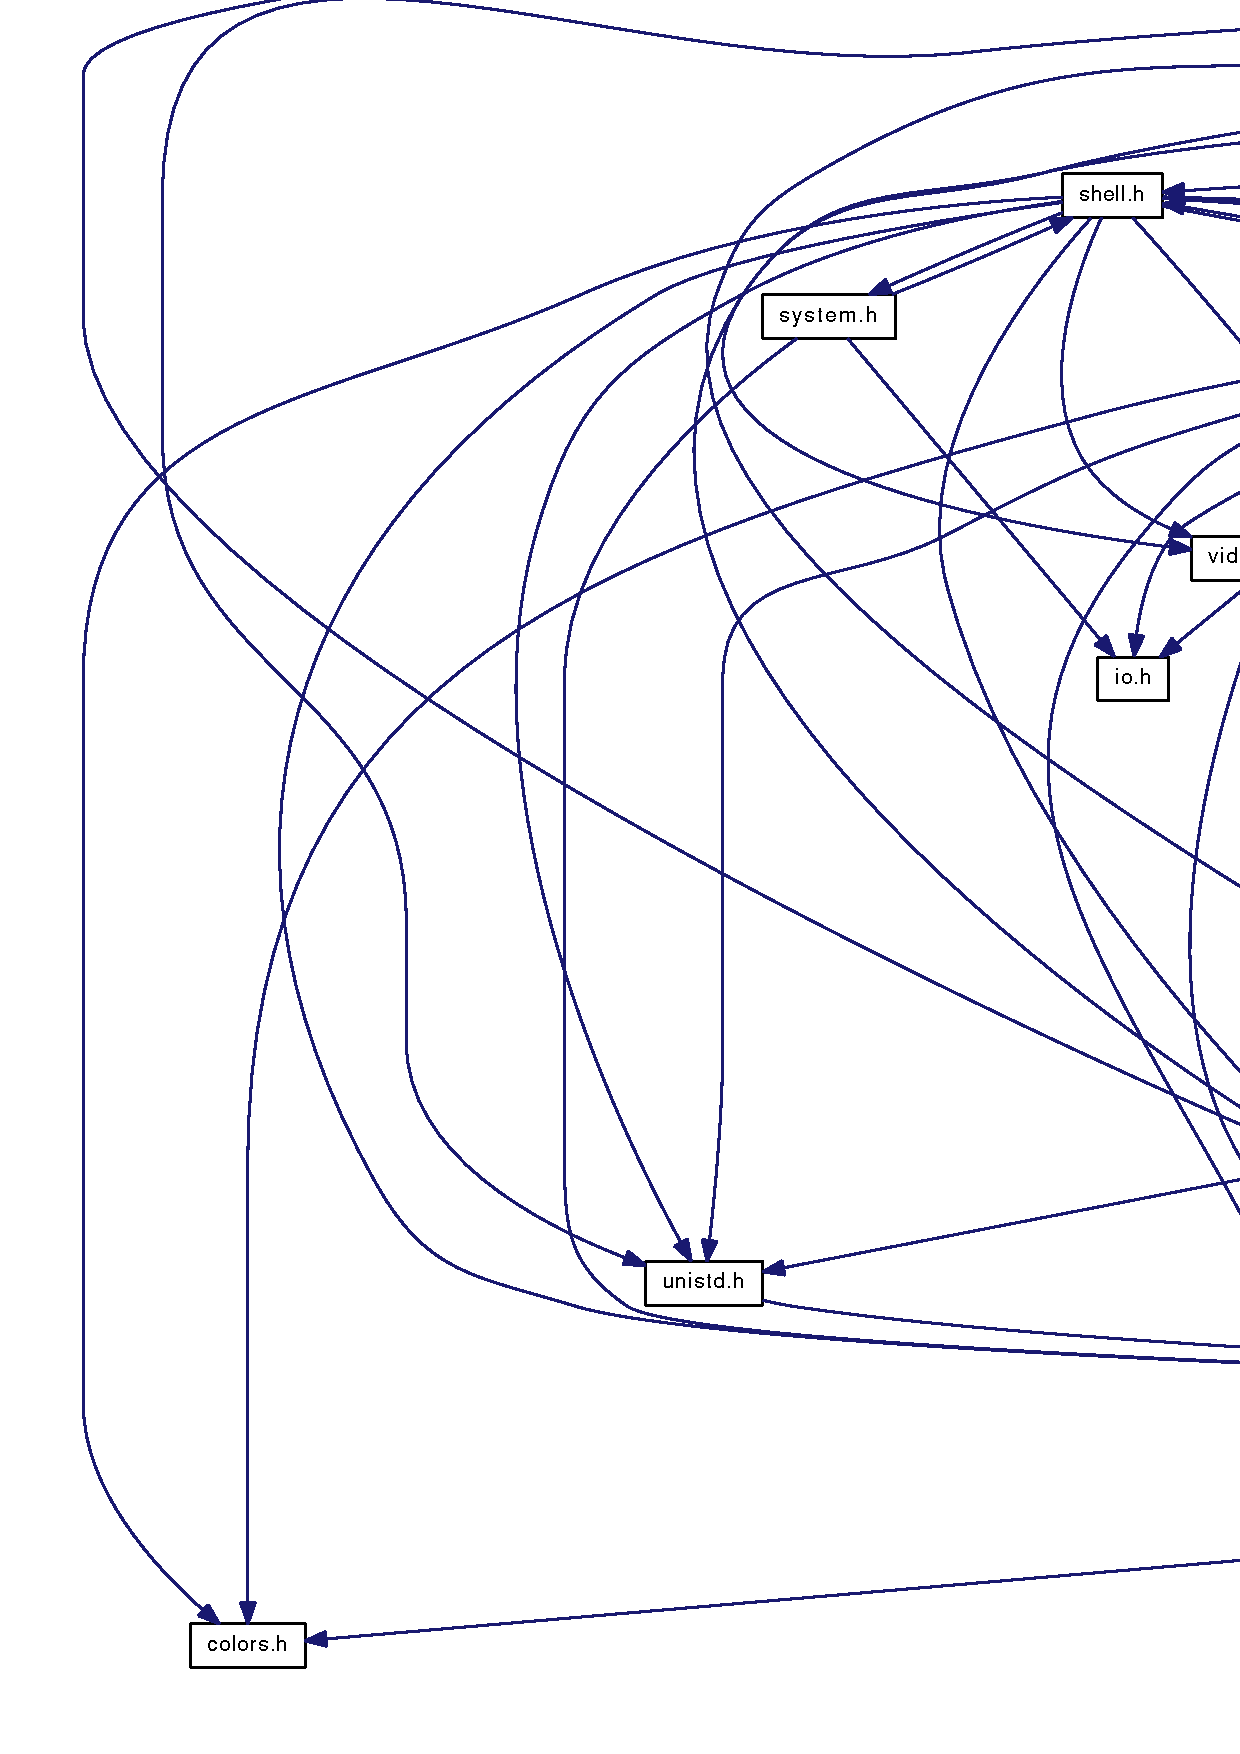
\includegraphics[width=420pt]{exceptions_8h__incl}
\end{center}
\end{figure}
This graph shows which files directly or indirectly include this file:\nopagebreak
\begin{figure}[H]
\begin{center}
\leavevmode
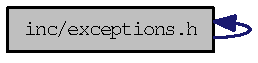
\includegraphics[width=80pt]{exceptions_8h__dep__incl}
\end{center}
\end{figure}
\subsection*{Functions}
\begin{DoxyCompactItemize}
\item 
void \hyperlink{exceptions_8h_a9a0ae2f785726650de9637601aa4c965}{loadExceptionHandlers} ()
\begin{DoxyCompactList}\small\item\em Loads the handler of the exception that was produced. \item\end{DoxyCompactList}\end{DoxyCompactItemize}


\subsection{Detailed Description}
Functions related with exception handling. \begin{DoxyAuthor}{Author}
Luciano Zemin, Nicolás Magni, Nicolás Purita 
\end{DoxyAuthor}


Definition in file \hyperlink{exceptions_8h_source}{exceptions.h}.



\subsection{Function Documentation}
\hypertarget{exceptions_8h_a9a0ae2f785726650de9637601aa4c965}{
\index{exceptions.h@{exceptions.h}!loadExceptionHandlers@{loadExceptionHandlers}}
\index{loadExceptionHandlers@{loadExceptionHandlers}!exceptions.h@{exceptions.h}}
\subsubsection[{loadExceptionHandlers}]{\setlength{\rightskip}{0pt plus 5cm}void loadExceptionHandlers ()}}
\label{exceptions_8h_a9a0ae2f785726650de9637601aa4c965}


Loads the handler of the exception that was produced. 



Definition at line 273 of file exceptions.c.



Here is the call graph for this function:\nopagebreak
\begin{figure}[H]
\begin{center}
\leavevmode
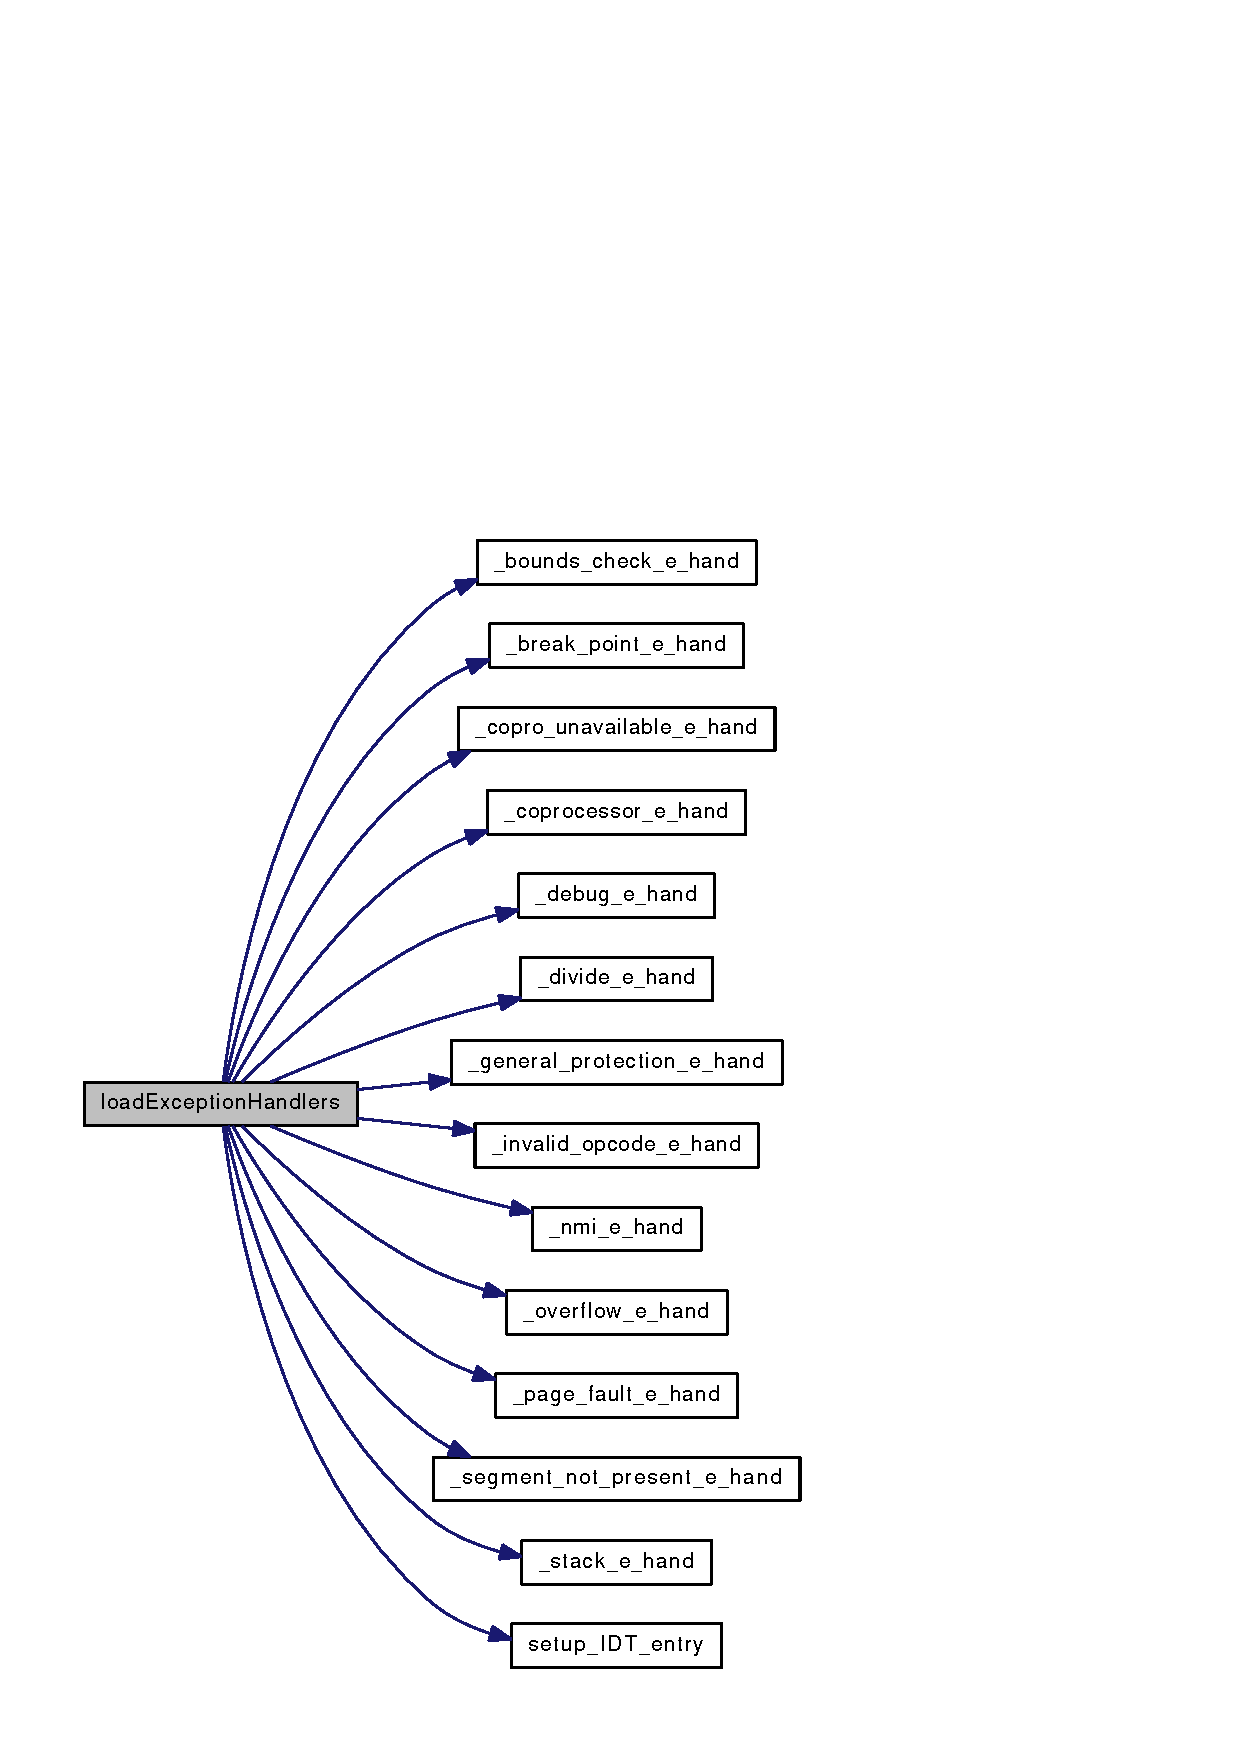
\includegraphics[width=194pt]{exceptions_8h_a9a0ae2f785726650de9637601aa4c965_cgraph}
\end{center}
\end{figure}




Here is the caller graph for this function:\nopagebreak
\begin{figure}[H]
\begin{center}
\leavevmode
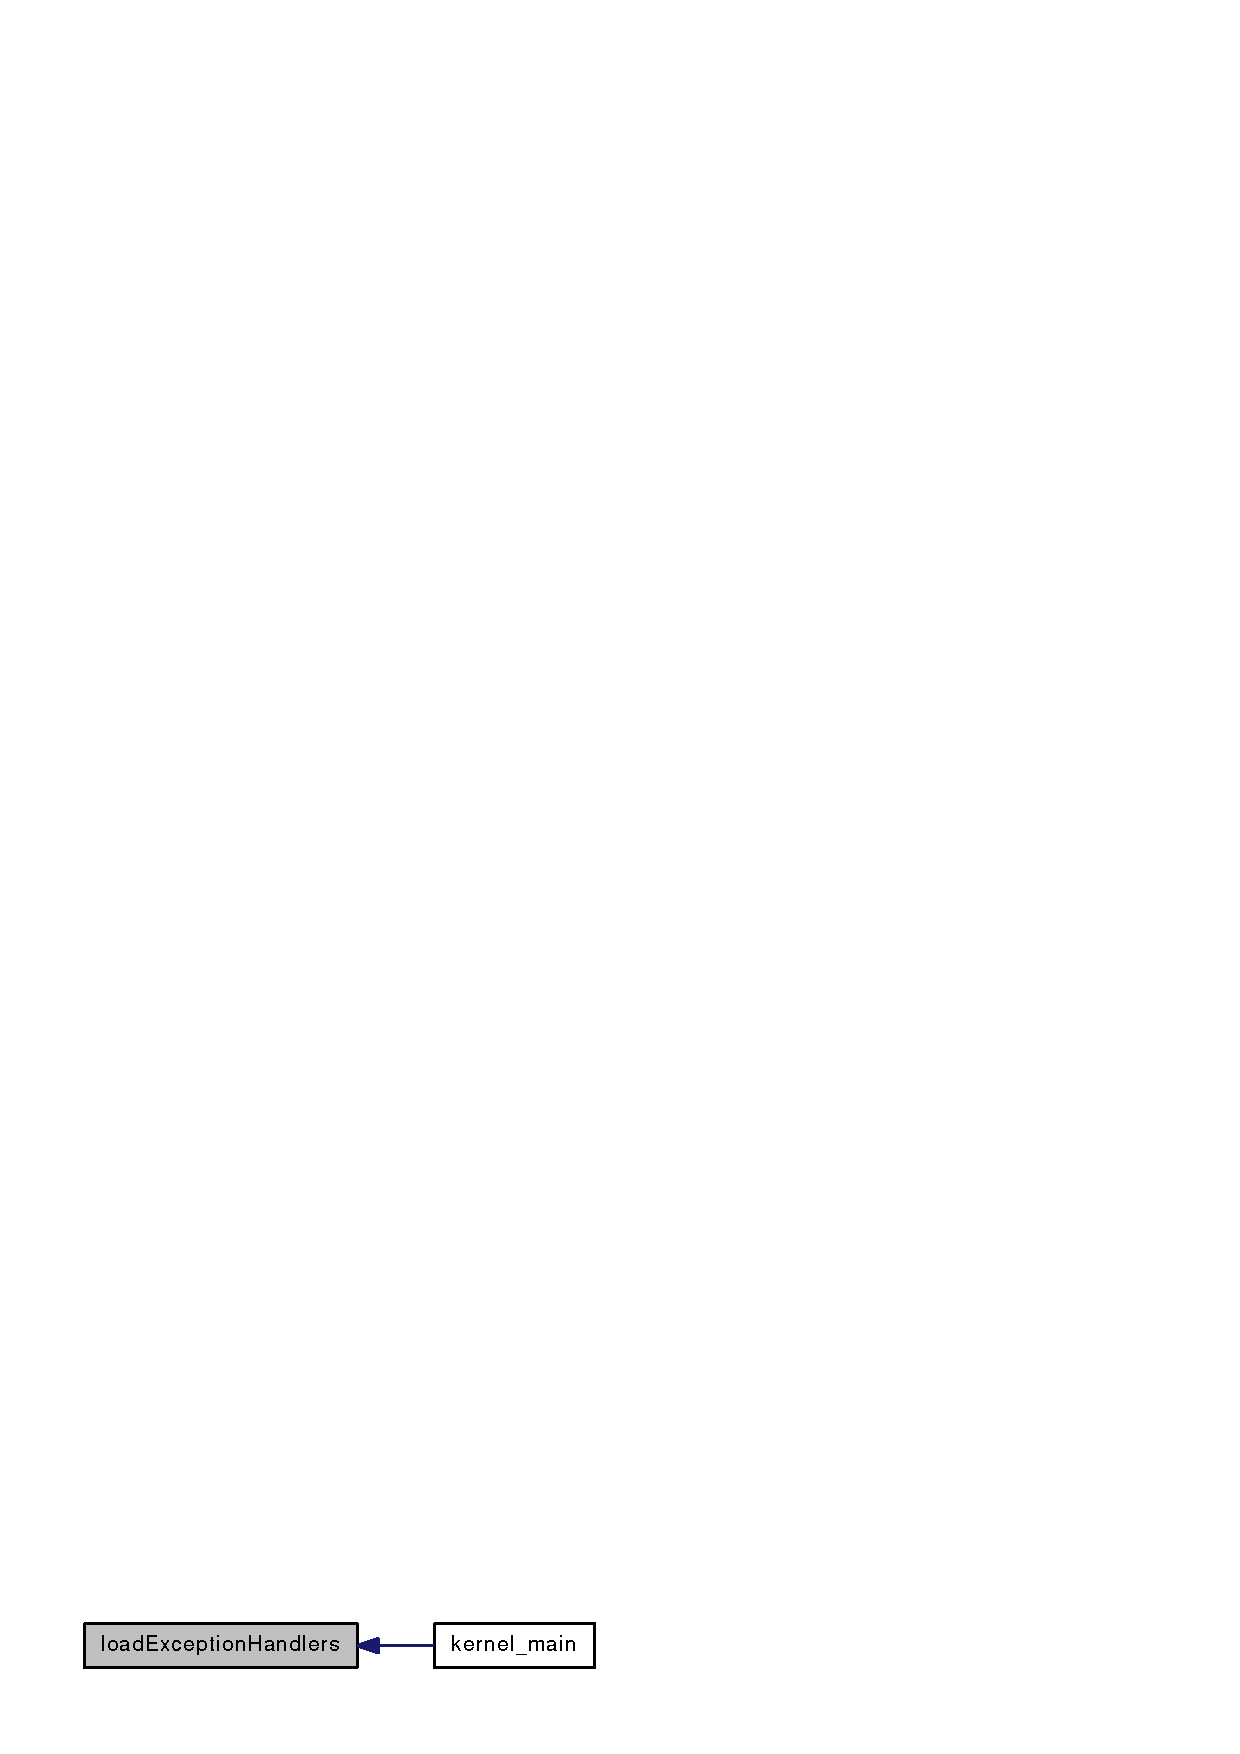
\includegraphics[width=145pt]{exceptions_8h_a9a0ae2f785726650de9637601aa4c965_icgraph}
\end{center}
\end{figure}



\hypertarget{grub_8inc}{
\section{inc/grub.inc File Reference}
\label{grub_8inc}\index{inc/grub.inc@{inc/grub.inc}}
}

\hypertarget{int80_8h}{
\section{inc/int80.h File Reference}
\label{int80_8h}\index{inc/int80.h@{inc/int80.h}}
}


int 80 generic calls.  


This graph shows which files directly or indirectly include this file:\nopagebreak
\begin{figure}[H]
\begin{center}
\leavevmode
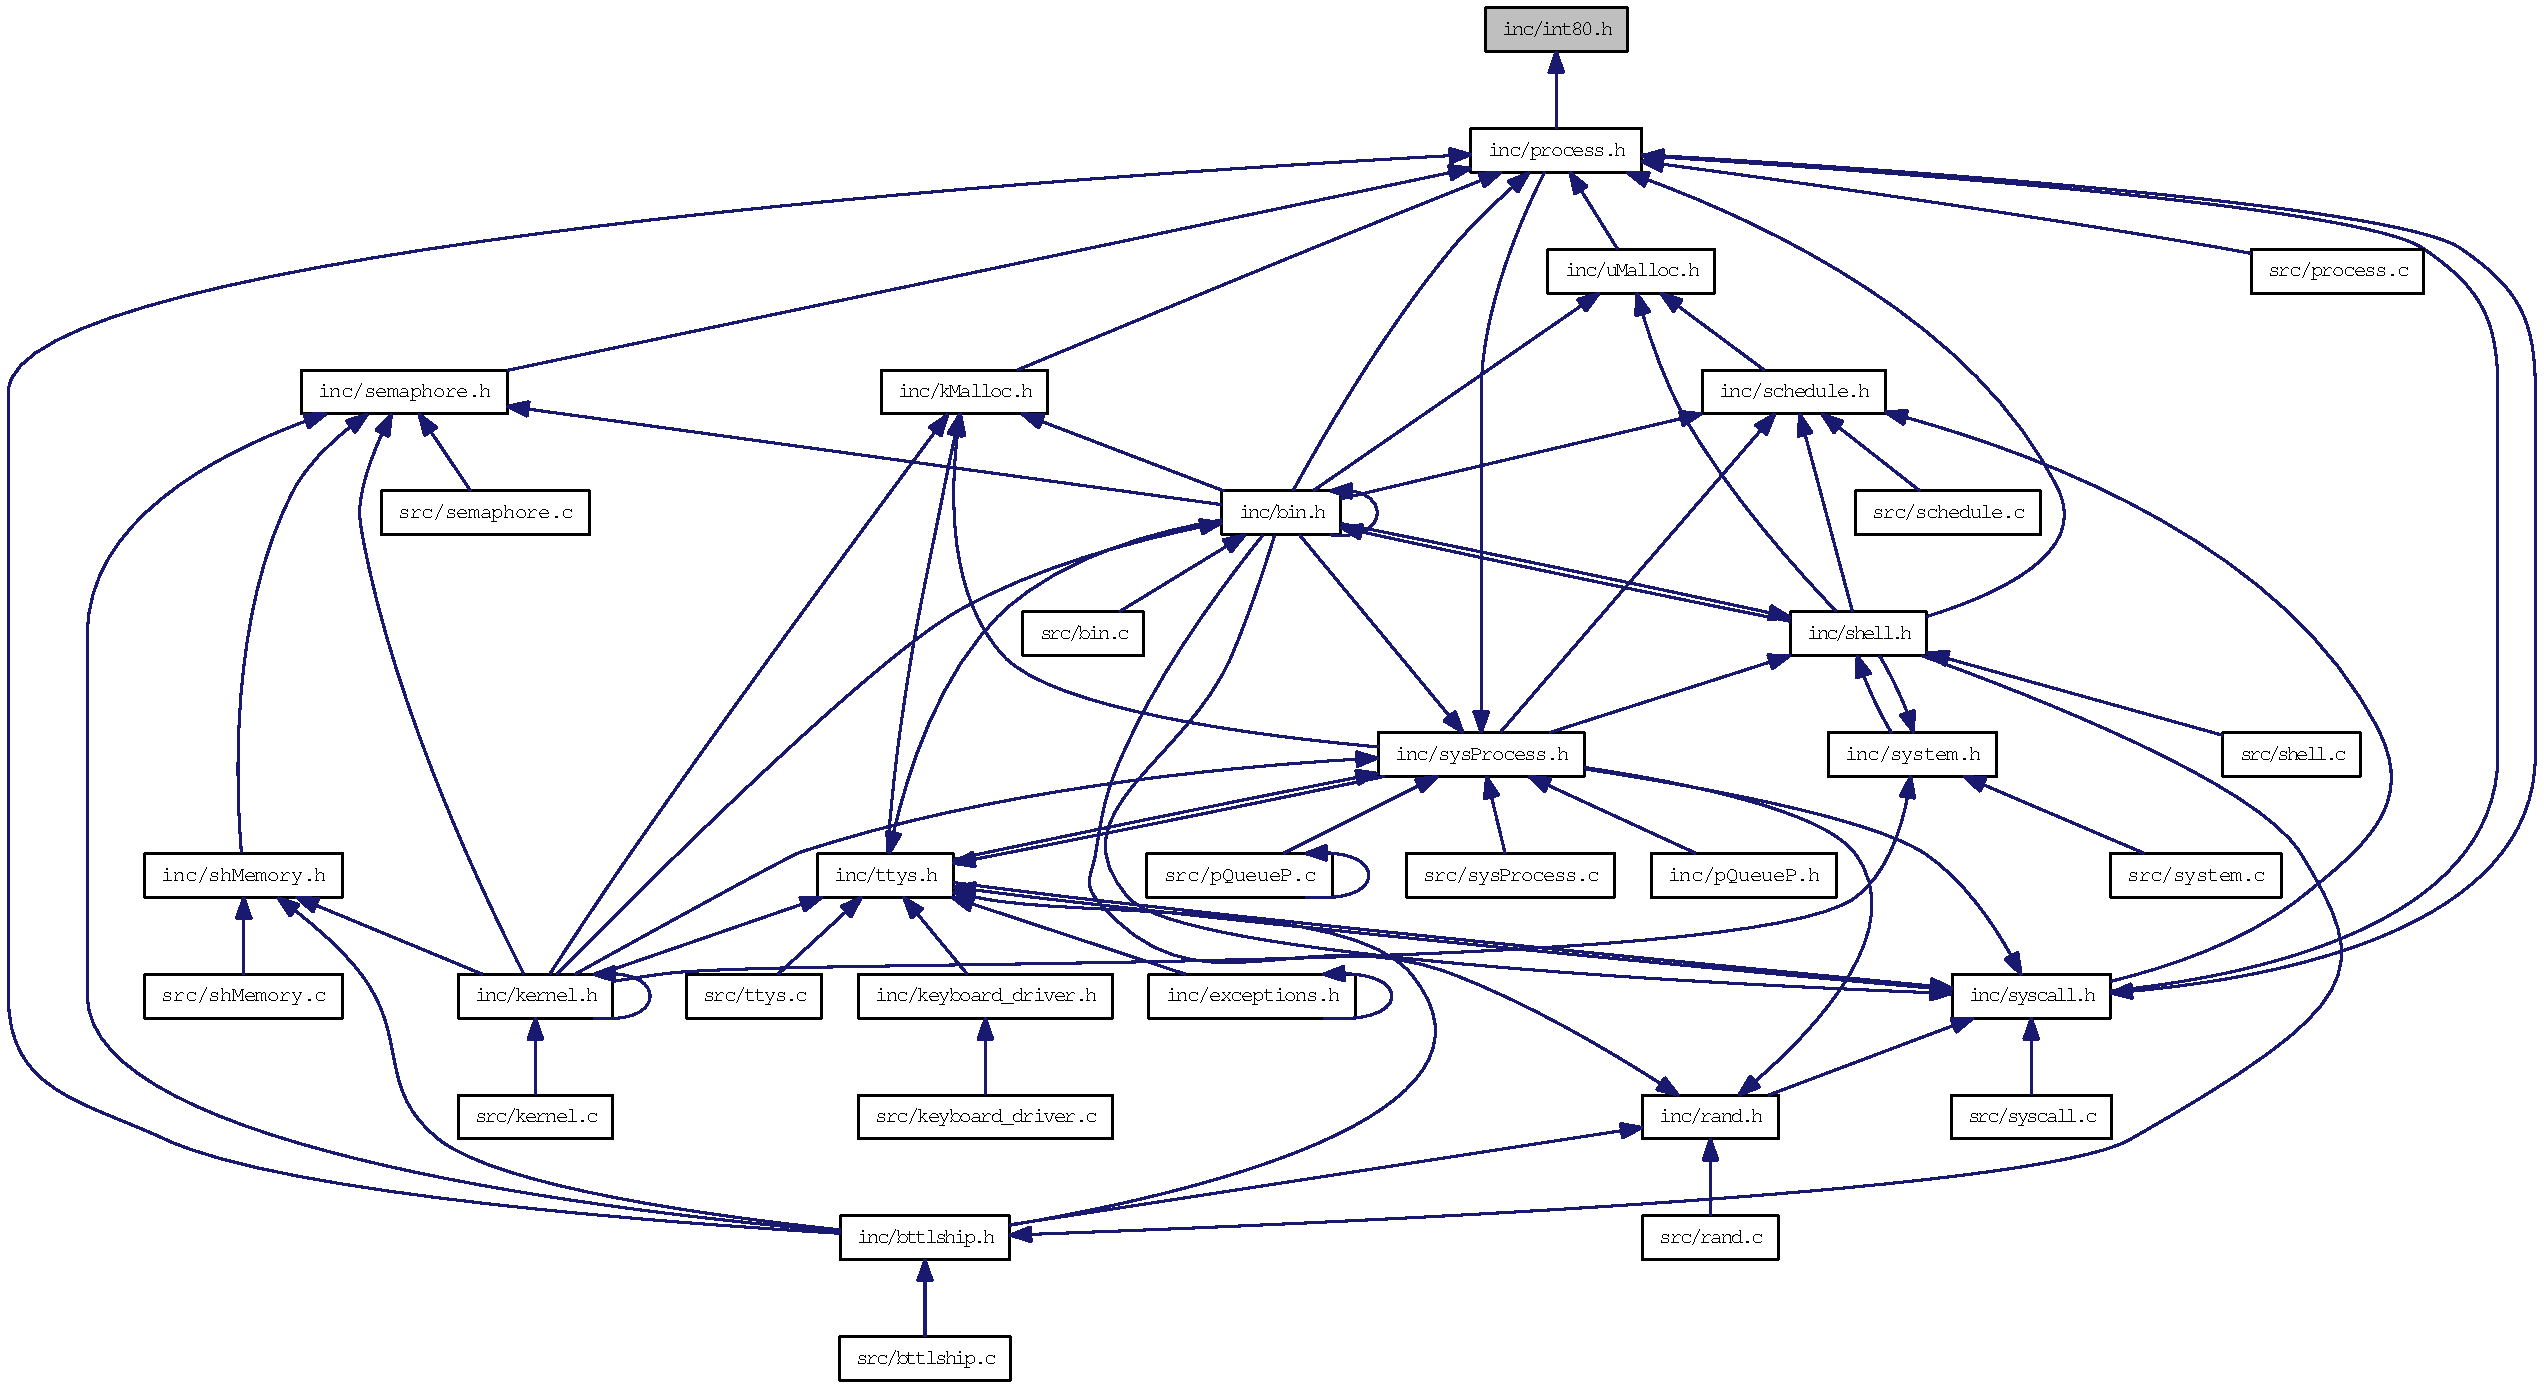
\includegraphics[width=420pt]{int80_8h__dep__incl}
\end{center}
\end{figure}
\subsection*{Functions}
\begin{DoxyCompactItemize}
\item 
void $\ast$ \hyperlink{int80_8h_a36ef33b2d2512c40b2aee77f85c56c38}{int80} (int eax, void $\ast$ebx, void $\ast$ecx, void $\ast$edx)
\begin{DoxyCompactList}\small\item\em copy the parameters to the processor registers. \item\end{DoxyCompactList}\item 
void $\ast$ \hyperlink{int80_8h_a68310308ad9c6753621ad8d0a790ddfd}{int80ext} (int eax, void $\ast$ebx, void $\ast$ecx, void $\ast$edx, void $\ast$edi, void $\ast$esi)
\begin{DoxyCompactList}\small\item\em copy the parameters to the processor registers. \item\end{DoxyCompactList}\end{DoxyCompactItemize}


\subsection{Detailed Description}
int 80 generic calls. \begin{DoxyAuthor}{Author}
Luciano Zemin, Nicolás Magni, Nicolás Purita 
\end{DoxyAuthor}


Definition in file \hyperlink{int80_8h_source}{int80.h}.



\subsection{Function Documentation}
\hypertarget{int80_8h_a36ef33b2d2512c40b2aee77f85c56c38}{
\index{int80.h@{int80.h}!int80@{int80}}
\index{int80@{int80}!int80.h@{int80.h}}
\subsubsection[{int80}]{\setlength{\rightskip}{0pt plus 5cm}void $\ast$ int80 (int {\em eax}, \/  void $\ast$ {\em ebx}, \/  void $\ast$ {\em ecx}, \/  void $\ast$ {\em edx})}}
\label{int80_8h_a36ef33b2d2512c40b2aee77f85c56c38}


copy the parameters to the processor registers. 


\begin{DoxyParams}{Parameters}
\item[{\em eax}]eax register. \item[{\em ebx}]ebx register. \item[{\em ecx}]ecx register. \item[{\em edx}]edx register.\end{DoxyParams}
\begin{DoxyReturn}{Returns}
The value returned by the function that the int 80 invoked. 
\end{DoxyReturn}


Here is the caller graph for this function:\nopagebreak
\begin{figure}[H]
\begin{center}
\leavevmode
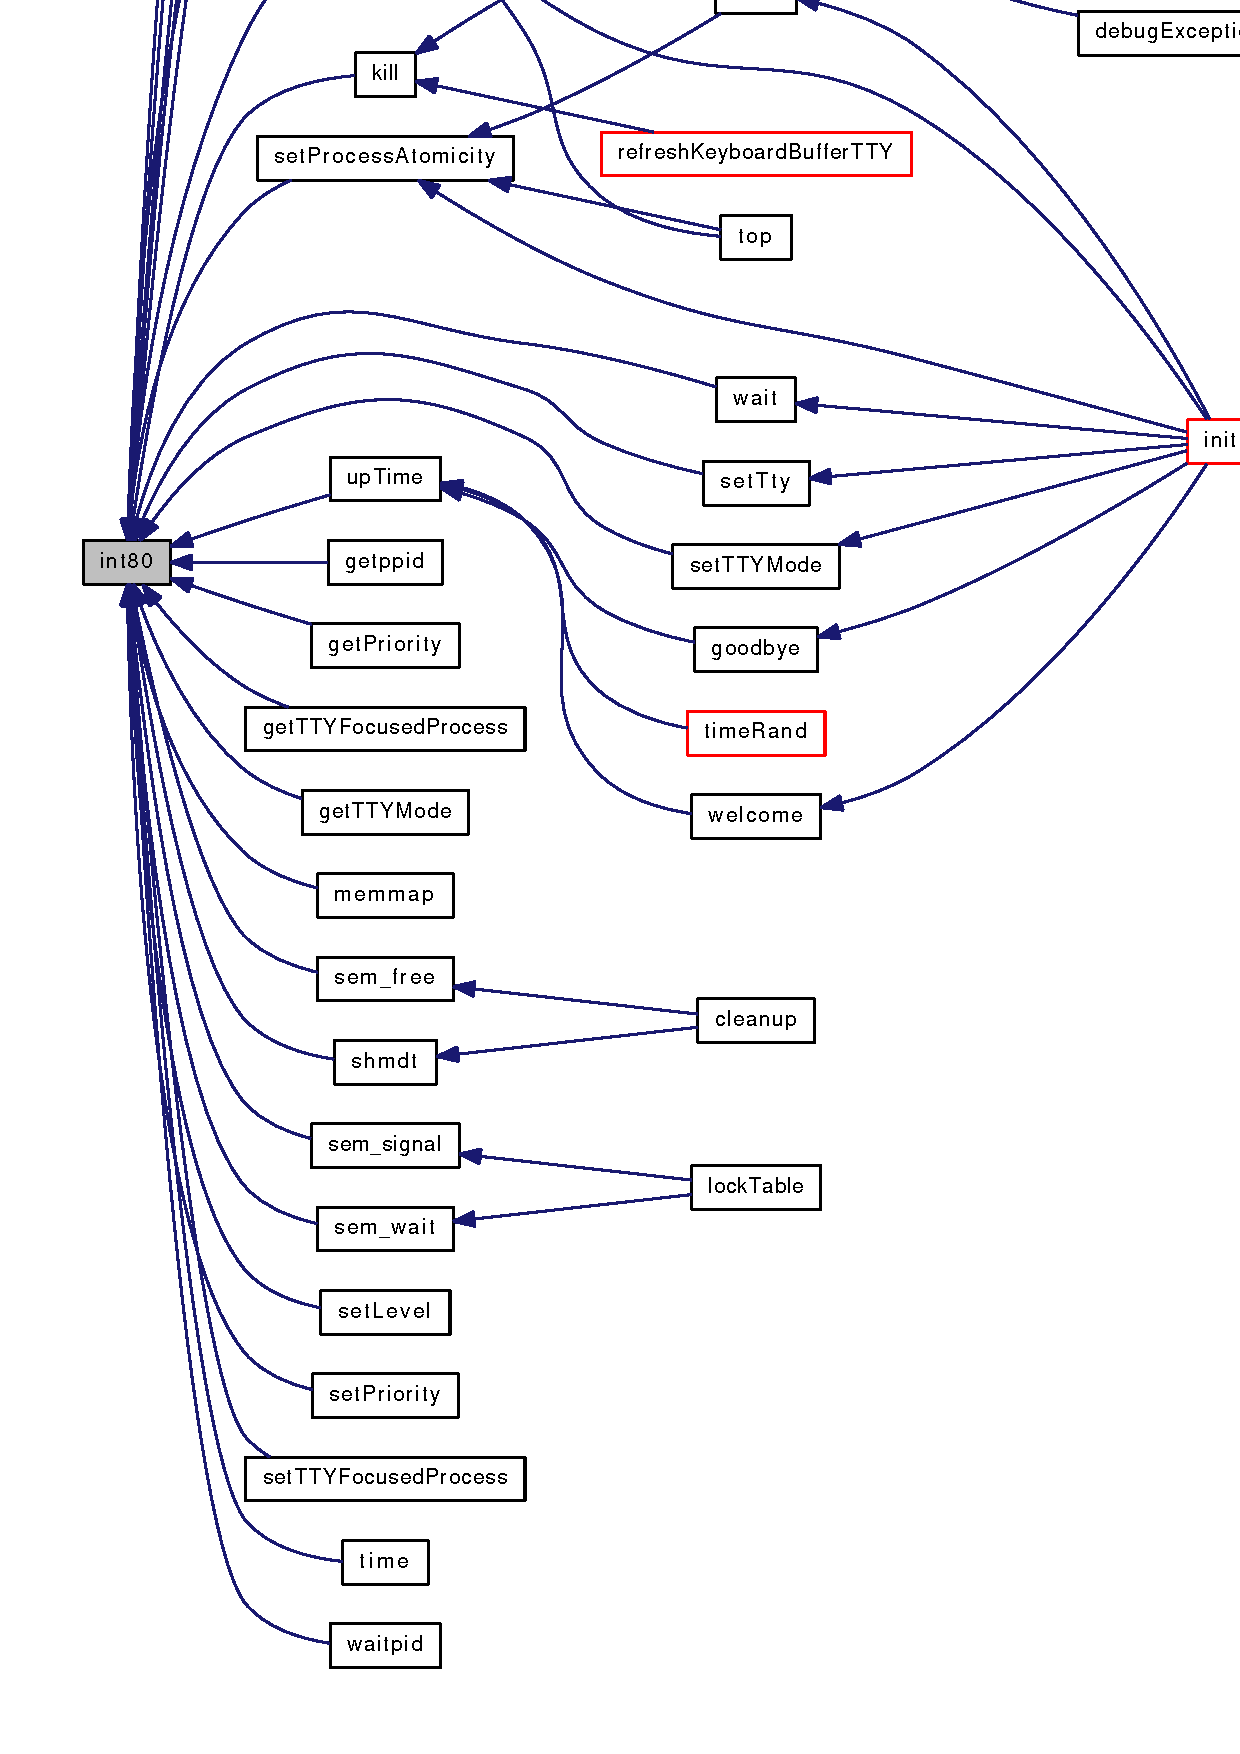
\includegraphics[width=351pt]{int80_8h_a36ef33b2d2512c40b2aee77f85c56c38_icgraph}
\end{center}
\end{figure}


\hypertarget{int80_8h_a68310308ad9c6753621ad8d0a790ddfd}{
\index{int80.h@{int80.h}!int80ext@{int80ext}}
\index{int80ext@{int80ext}!int80.h@{int80.h}}
\subsubsection[{int80ext}]{\setlength{\rightskip}{0pt plus 5cm}void $\ast$ int80ext (int {\em eax}, \/  void $\ast$ {\em ebx}, \/  void $\ast$ {\em ecx}, \/  void $\ast$ {\em edx}, \/  void $\ast$ {\em edi}, \/  void $\ast$ {\em esi})}}
\label{int80_8h_a68310308ad9c6753621ad8d0a790ddfd}


copy the parameters to the processor registers. 


\begin{DoxyParams}{Parameters}
\item[{\em eax}]eax register. \item[{\em ebx}]ebx register. \item[{\em ecx}]ecx register. \item[{\em edx}]edx register. \item[{\em edi}]edi register. \item[{\em esi}]esi register.\end{DoxyParams}
\begin{DoxyReturn}{Returns}
The value returned by the function that the int 80 invoked. 
\end{DoxyReturn}


Here is the caller graph for this function:\nopagebreak
\begin{figure}[H]
\begin{center}
\leavevmode
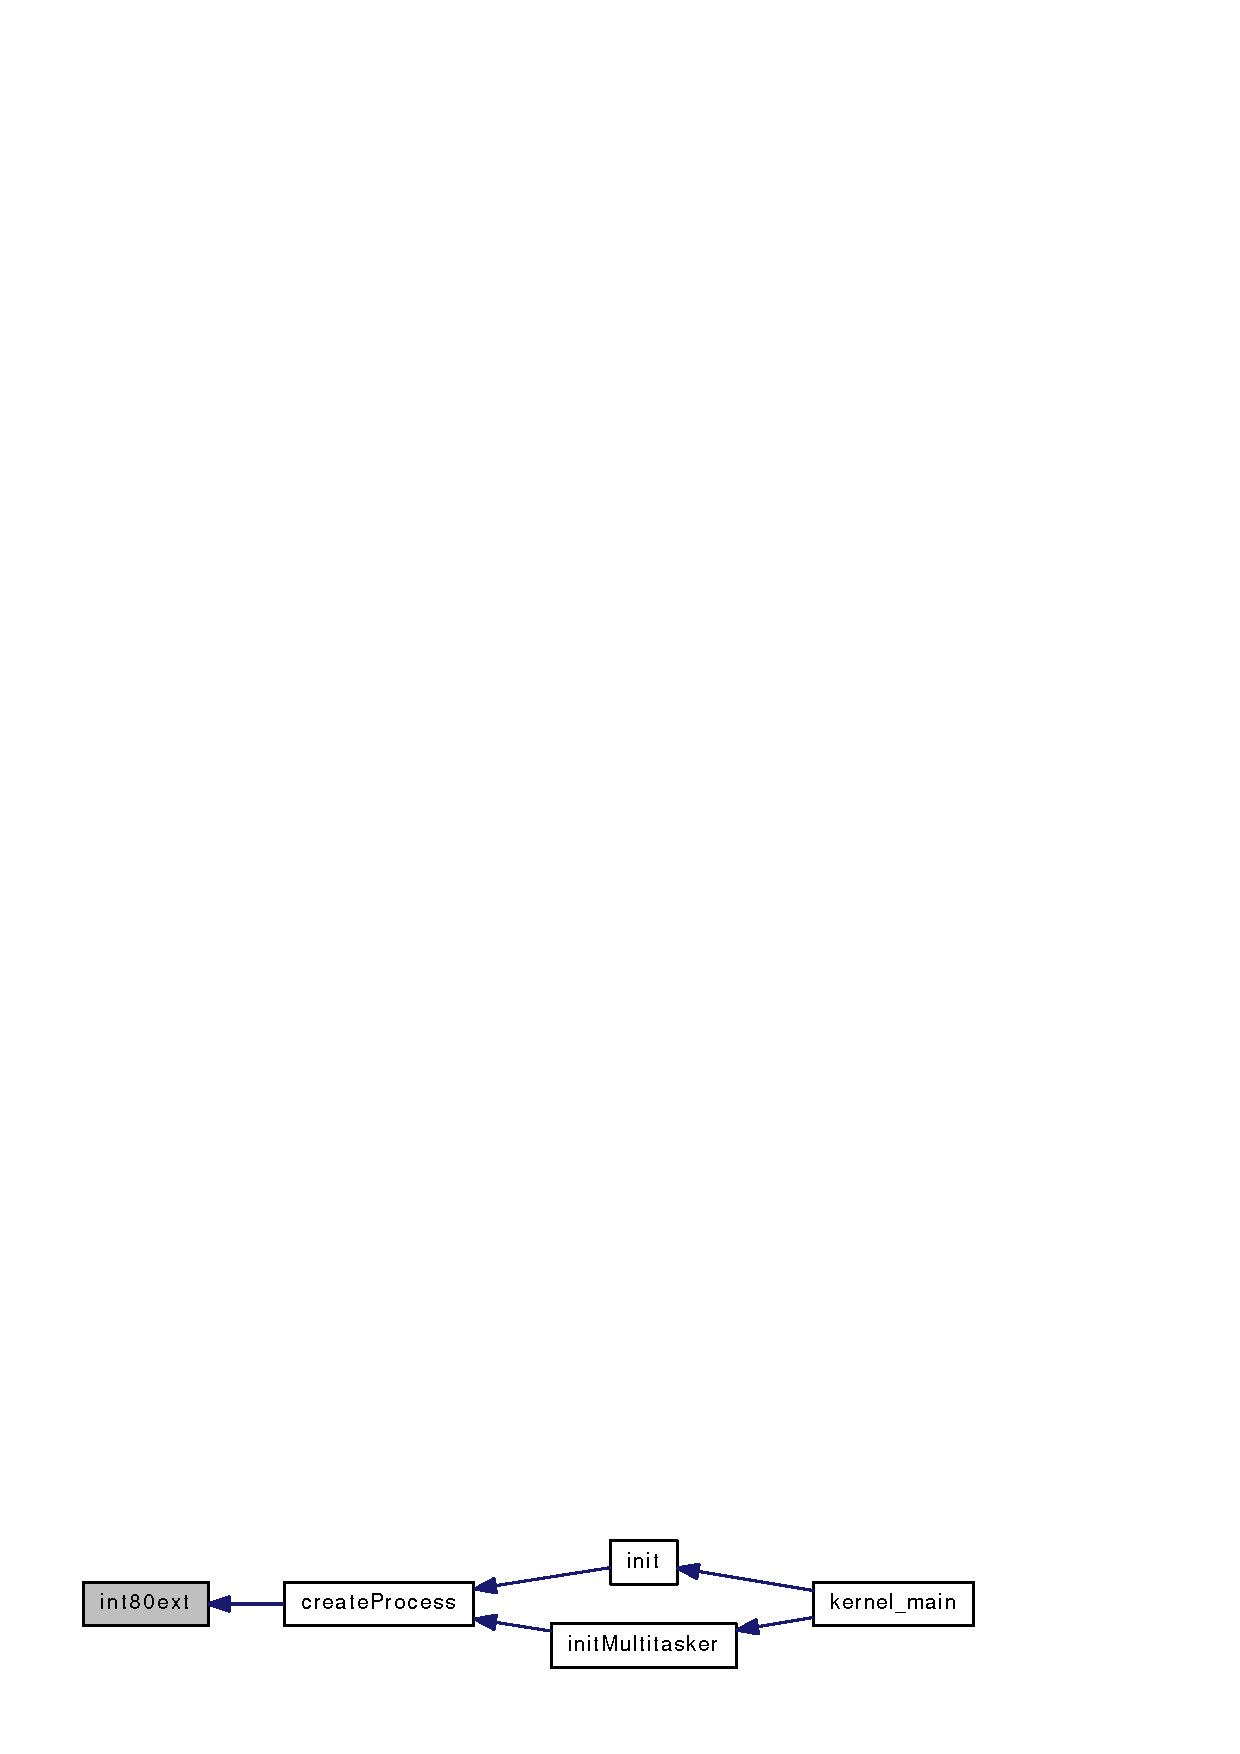
\includegraphics[width=236pt]{int80_8h_a68310308ad9c6753621ad8d0a790ddfd_icgraph}
\end{center}
\end{figure}



\hypertarget{int__handlers_8h}{
\section{inc/int\_\-handlers.h File Reference}
\label{int__handlers_8h}\index{inc/int\_\-handlers.h@{inc/int\_\-handlers.h}}
}


Declarations of all interrupt handlers.  


\subsection*{Functions}
\begin{DoxyCompactItemize}
\item 
void \hyperlink{int__handlers_8h_abe15fe9e35457aba9d9be21b7fc035c8}{\_\-int\_\-08\_\-handler} (void)
\begin{DoxyCompactList}\small\item\em This function handles the timer tick interrupt. \item\end{DoxyCompactList}\item 
void \hyperlink{int__handlers_8h_aa3e8e59826d84280a1918b493750305f}{\_\-int\_\-80\_\-handler} (void)
\begin{DoxyCompactList}\small\item\em This function handles the kernel system calls. Posible system calls: \_\-SYS\_\-WRITE \_\-SYS\_\-READ This rutine must be load into the IDT in the position 0x80. \item\end{DoxyCompactList}\item 
void \hyperlink{int__handlers_8h_ad4d015f51393b56a91f3aae98675a1f3}{\_\-int\_\-09\_\-handler} (void)
\begin{DoxyCompactList}\small\item\em This function handles the keyboard interrupt. \item\end{DoxyCompactList}\end{DoxyCompactItemize}


\subsection{Detailed Description}
Declarations of all interrupt handlers. \begin{DoxyAuthor}{Author}
Luciano Zemin, Nicolás Magni, Nicolás Purita 
\end{DoxyAuthor}


Definition in file \hyperlink{int__handlers_8h_source}{int\_\-handlers.h}.



\subsection{Function Documentation}
\hypertarget{int__handlers_8h_abe15fe9e35457aba9d9be21b7fc035c8}{
\index{int\_\-handlers.h@{int\_\-handlers.h}!\_\-int\_\-08\_\-handler@{\_\-int\_\-08\_\-handler}}
\index{\_\-int\_\-08\_\-handler@{\_\-int\_\-08\_\-handler}!int_handlers.h@{int\_\-handlers.h}}
\subsubsection[{\_\-int\_\-08\_\-handler}]{\setlength{\rightskip}{0pt plus 5cm}void \_\-int\_\-08\_\-handler (void)}}
\label{int__handlers_8h_abe15fe9e35457aba9d9be21b7fc035c8}


This function handles the timer tick interrupt. 



Here is the caller graph for this function:\nopagebreak
\begin{figure}[H]
\begin{center}
\leavevmode
\includegraphics[width=127pt]{int__handlers_8h_abe15fe9e35457aba9d9be21b7fc035c8_icgraph}
\end{center}
\end{figure}


\hypertarget{int__handlers_8h_ad4d015f51393b56a91f3aae98675a1f3}{
\index{int\_\-handlers.h@{int\_\-handlers.h}!\_\-int\_\-09\_\-handler@{\_\-int\_\-09\_\-handler}}
\index{\_\-int\_\-09\_\-handler@{\_\-int\_\-09\_\-handler}!int_handlers.h@{int\_\-handlers.h}}
\subsubsection[{\_\-int\_\-09\_\-handler}]{\setlength{\rightskip}{0pt plus 5cm}void \_\-int\_\-09\_\-handler (void)}}
\label{int__handlers_8h_ad4d015f51393b56a91f3aae98675a1f3}


This function handles the keyboard interrupt. 



Here is the caller graph for this function:\nopagebreak
\begin{figure}[H]
\begin{center}
\leavevmode
\includegraphics[width=127pt]{int__handlers_8h_ad4d015f51393b56a91f3aae98675a1f3_icgraph}
\end{center}
\end{figure}


\hypertarget{int__handlers_8h_aa3e8e59826d84280a1918b493750305f}{
\index{int\_\-handlers.h@{int\_\-handlers.h}!\_\-int\_\-80\_\-handler@{\_\-int\_\-80\_\-handler}}
\index{\_\-int\_\-80\_\-handler@{\_\-int\_\-80\_\-handler}!int_handlers.h@{int\_\-handlers.h}}
\subsubsection[{\_\-int\_\-80\_\-handler}]{\setlength{\rightskip}{0pt plus 5cm}void \_\-int\_\-80\_\-handler (void)}}
\label{int__handlers_8h_aa3e8e59826d84280a1918b493750305f}


This function handles the kernel system calls. Posible system calls: \_\-SYS\_\-WRITE \_\-SYS\_\-READ This rutine must be load into the IDT in the position 0x80. 



Here is the caller graph for this function:\nopagebreak
\begin{figure}[H]
\begin{center}
\leavevmode
\includegraphics[width=127pt]{int__handlers_8h_aa3e8e59826d84280a1918b493750305f_icgraph}
\end{center}
\end{figure}



\hypertarget{io_8h}{
\section{inc/io.h File Reference}
\label{io_8h}\index{inc/io.h@{inc/io.h}}
}


Declaration of functions and constants related with direct access to hardware.  


This graph shows which files directly or indirectly include this file:\nopagebreak
\begin{figure}[H]
\begin{center}
\leavevmode
\includegraphics[width=420pt]{io_8h__dep__incl}
\end{center}
\end{figure}
\subsection*{Defines}
\begin{DoxyCompactItemize}
\item 
\#define \hyperlink{io_8h_a20cb09d28af0835280c004e0030d0ba4}{VIDEO\_\-MEMORY\_\-ADDRESS}~(void $\ast$)0xB8000
\end{DoxyCompactItemize}
\subsection*{Functions}
\begin{DoxyCompactItemize}
\item 
int \hyperlink{io_8h_ac17a6cfbeef702c55063c3350220c126}{inportb} (int port)
\begin{DoxyCompactList}\small\item\em This function grabs the value stored in the given port. \item\end{DoxyCompactList}\item 
void \hyperlink{io_8h_a816f57bd2dc5cfc848e5f6954476844c}{outportb} (int port, int value)
\begin{DoxyCompactList}\small\item\em This function stores the given value in the given port. \item\end{DoxyCompactList}\end{DoxyCompactItemize}


\subsection{Detailed Description}
Declaration of functions and constants related with direct access to hardware. \begin{DoxyAuthor}{Author}
Luciano Zemin, Nicolás Magni, Nicolás Purita 
\end{DoxyAuthor}


Definition in file \hyperlink{io_8h_source}{io.h}.



\subsection{Define Documentation}
\hypertarget{io_8h_a20cb09d28af0835280c004e0030d0ba4}{
\index{io.h@{io.h}!VIDEO\_\-MEMORY\_\-ADDRESS@{VIDEO\_\-MEMORY\_\-ADDRESS}}
\index{VIDEO\_\-MEMORY\_\-ADDRESS@{VIDEO\_\-MEMORY\_\-ADDRESS}!io.h@{io.h}}
\subsubsection[{VIDEO\_\-MEMORY\_\-ADDRESS}]{\setlength{\rightskip}{0pt plus 5cm}\#define VIDEO\_\-MEMORY\_\-ADDRESS~(void $\ast$)0xB8000}}
\label{io_8h_a20cb09d28af0835280c004e0030d0ba4}


Definition at line 17 of file io.h.



\subsection{Function Documentation}
\hypertarget{io_8h_ac17a6cfbeef702c55063c3350220c126}{
\index{io.h@{io.h}!inportb@{inportb}}
\index{inportb@{inportb}!io.h@{io.h}}
\subsubsection[{inportb}]{\setlength{\rightskip}{0pt plus 5cm}int inportb (int {\em port})}}
\label{io_8h_ac17a6cfbeef702c55063c3350220c126}


This function grabs the value stored in the given port. 


\begin{DoxyParams}{Parameters}
\item[{\em port}]The desired port number. \end{DoxyParams}
\begin{DoxyReturn}{Returns}
This function returns an int instance with the value obtained.
\end{DoxyReturn}

\begin{DoxyCode}
                        int value;
                        value = inport(0x60);
\end{DoxyCode}


\begin{DoxySeeAlso}{See also}
outport() 
\end{DoxySeeAlso}


Here is the caller graph for this function:\nopagebreak
\begin{figure}[H]
\begin{center}
\leavevmode
\includegraphics[width=225pt]{io_8h_ac17a6cfbeef702c55063c3350220c126_icgraph}
\end{center}
\end{figure}


\hypertarget{io_8h_a816f57bd2dc5cfc848e5f6954476844c}{
\index{io.h@{io.h}!outportb@{outportb}}
\index{outportb@{outportb}!io.h@{io.h}}
\subsubsection[{outportb}]{\setlength{\rightskip}{0pt plus 5cm}void outportb (int {\em port}, \/  int {\em value})}}
\label{io_8h_a816f57bd2dc5cfc848e5f6954476844c}


This function stores the given value in the given port. 


\begin{DoxyParams}{Parameters}
\item[{\em port}]Desired port number. \item[{\em value}]Desired value to set.\end{DoxyParams}

\begin{DoxyCode}
                        outport (0x64, 0x31)
\end{DoxyCode}


\begin{DoxySeeAlso}{See also}
inport() 
\end{DoxySeeAlso}


Here is the caller graph for this function:\nopagebreak
\begin{figure}[H]
\begin{center}
\leavevmode
\includegraphics[width=230pt]{io_8h_a816f57bd2dc5cfc848e5f6954476844c_icgraph}
\end{center}
\end{figure}



\hypertarget{kasm_8h}{
\section{inc/kasm.h File Reference}
\label{kasm_8h}\index{inc/kasm.h@{inc/kasm.h}}
}


Kernel utilities.  


{\ttfamily \#include \char`\"{}types.h\char`\"{}}\par
Include dependency graph for kasm.h:\nopagebreak
\begin{figure}[H]
\begin{center}
\leavevmode
\includegraphics[width=82pt]{kasm_8h__incl}
\end{center}
\end{figure}
This graph shows which files directly or indirectly include this file:\nopagebreak
\begin{figure}[H]
\begin{center}
\leavevmode
\includegraphics[width=420pt]{kasm_8h__dep__incl}
\end{center}
\end{figure}
\subsection*{Functions}
\begin{DoxyCompactItemize}
\item 
unsigned int \hyperlink{kasm_8h_a05d80083a9d438f00302b89cce618ca5}{\_\-read\_\-msw} ()
\begin{DoxyCompactList}\small\item\em Brief. \item\end{DoxyCompactList}\item 
void \hyperlink{kasm_8h_ae8fa119f684ecab085b10ac3057a7dfc}{\_\-lidt} (\hyperlink{struct_i_d_t_r}{IDTR} $\ast$\hyperlink{kernel_8c_afefc9bc7f2fa69f8a1f6e35c2e804260}{idtr})
\begin{DoxyCompactList}\small\item\em Brief. \item\end{DoxyCompactList}\item 
void \hyperlink{kasm_8h_a040f3ed216543a3a9ddebd17f2b2bcd0}{\_\-mascaraPIC1} (byte mascara)
\begin{DoxyCompactList}\small\item\em Brief. \item\end{DoxyCompactList}\item 
void \hyperlink{kasm_8h_a7bcff8af975befd9654311a14bde1098}{\_\-mascaraPIC2} (byte mascara)
\begin{DoxyCompactList}\small\item\em Brief. \item\end{DoxyCompactList}\item 
void \hyperlink{kasm_8h_adc8888227cfbdfe307b5b5bd0ee5c80a}{\_\-Cli} (void)
\begin{DoxyCompactList}\small\item\em Brief. \item\end{DoxyCompactList}\item 
void \hyperlink{kasm_8h_a38b31cfe95df07495ffe67cc0b6a9c5d}{\_\-Sti} (void)
\begin{DoxyCompactList}\small\item\em Brief. \item\end{DoxyCompactList}\item 
void \hyperlink{kasm_8h_a105ee6e3dedbb5d51a31bc66ac4c5edf}{\_\-debug} (void)
\begin{DoxyCompactList}\small\item\em Brief. \item\end{DoxyCompactList}\item 
unsigned \hyperlink{kasm_8h_ae933e936bb66cef841f7e5ea9733cc09}{getCodeSegment} ()
\begin{DoxyCompactList}\small\item\em Brief. \item\end{DoxyCompactList}\end{DoxyCompactItemize}


\subsection{Detailed Description}
Kernel utilities. \begin{DoxyAuthor}{Author}
Luciano Zemin, Nicolás Magni, Nicolás Purita 
\end{DoxyAuthor}


Definition in file \hyperlink{kasm_8h_source}{kasm.h}.



\subsection{Function Documentation}
\hypertarget{kasm_8h_adc8888227cfbdfe307b5b5bd0ee5c80a}{
\index{kasm.h@{kasm.h}!\_\-Cli@{\_\-Cli}}
\index{\_\-Cli@{\_\-Cli}!kasm.h@{kasm.h}}
\subsubsection[{\_\-Cli}]{\setlength{\rightskip}{0pt plus 5cm}void \_\-Cli (void)}}
\label{kasm_8h_adc8888227cfbdfe307b5b5bd0ee5c80a}


Brief. 

Use: 
\begin{DoxyCode}
\end{DoxyCode}


\begin{DoxySeeAlso}{See also}
f1() f2() 
\end{DoxySeeAlso}


Here is the caller graph for this function:\nopagebreak
\begin{figure}[H]
\begin{center}
\leavevmode
\includegraphics[width=96pt]{kasm_8h_adc8888227cfbdfe307b5b5bd0ee5c80a_icgraph}
\end{center}
\end{figure}


\hypertarget{kasm_8h_a105ee6e3dedbb5d51a31bc66ac4c5edf}{
\index{kasm.h@{kasm.h}!\_\-debug@{\_\-debug}}
\index{\_\-debug@{\_\-debug}!kasm.h@{kasm.h}}
\subsubsection[{\_\-debug}]{\setlength{\rightskip}{0pt plus 5cm}void \_\-debug (void)}}
\label{kasm_8h_a105ee6e3dedbb5d51a31bc66ac4c5edf}


Brief. 

Use: 
\begin{DoxyCode}
\end{DoxyCode}


\begin{DoxySeeAlso}{See also}
f1() f2() 
\end{DoxySeeAlso}
\hypertarget{kasm_8h_ae8fa119f684ecab085b10ac3057a7dfc}{
\index{kasm.h@{kasm.h}!\_\-lidt@{\_\-lidt}}
\index{\_\-lidt@{\_\-lidt}!kasm.h@{kasm.h}}
\subsubsection[{\_\-lidt}]{\setlength{\rightskip}{0pt plus 5cm}void \_\-lidt ({\bf IDTR} $\ast$ {\em idtr})}}
\label{kasm_8h_ae8fa119f684ecab085b10ac3057a7dfc}


Brief. 


\begin{DoxyParams}{Parameters}
\item[{\em idtr}]ParamBrief.\end{DoxyParams}
Use: 
\begin{DoxyCode}
\end{DoxyCode}


\begin{DoxySeeAlso}{See also}
f1() f2() 
\end{DoxySeeAlso}


Here is the caller graph for this function:\nopagebreak
\begin{figure}[H]
\begin{center}
\leavevmode
\includegraphics[width=98pt]{kasm_8h_ae8fa119f684ecab085b10ac3057a7dfc_icgraph}
\end{center}
\end{figure}


\hypertarget{kasm_8h_a040f3ed216543a3a9ddebd17f2b2bcd0}{
\index{kasm.h@{kasm.h}!\_\-mascaraPIC1@{\_\-mascaraPIC1}}
\index{\_\-mascaraPIC1@{\_\-mascaraPIC1}!kasm.h@{kasm.h}}
\subsubsection[{\_\-mascaraPIC1}]{\setlength{\rightskip}{0pt plus 5cm}void \_\-mascaraPIC1 (byte {\em mascara})}}
\label{kasm_8h_a040f3ed216543a3a9ddebd17f2b2bcd0}


Brief. 


\begin{DoxyParams}{Parameters}
\item[{\em mascara}]ParamBrief.\end{DoxyParams}
Use: 
\begin{DoxyCode}
\end{DoxyCode}


\begin{DoxySeeAlso}{See also}
f1() f2() 
\end{DoxySeeAlso}


Here is the caller graph for this function:\nopagebreak
\begin{figure}[H]
\begin{center}
\leavevmode
\includegraphics[width=123pt]{kasm_8h_a040f3ed216543a3a9ddebd17f2b2bcd0_icgraph}
\end{center}
\end{figure}


\hypertarget{kasm_8h_a7bcff8af975befd9654311a14bde1098}{
\index{kasm.h@{kasm.h}!\_\-mascaraPIC2@{\_\-mascaraPIC2}}
\index{\_\-mascaraPIC2@{\_\-mascaraPIC2}!kasm.h@{kasm.h}}
\subsubsection[{\_\-mascaraPIC2}]{\setlength{\rightskip}{0pt plus 5cm}void \_\-mascaraPIC2 (byte {\em mascara})}}
\label{kasm_8h_a7bcff8af975befd9654311a14bde1098}


Brief. 


\begin{DoxyParams}{Parameters}
\item[{\em mascara}]ParamBrief.\end{DoxyParams}
Use: 
\begin{DoxyCode}
\end{DoxyCode}


\begin{DoxySeeAlso}{See also}
f1() f2() 
\end{DoxySeeAlso}


Here is the caller graph for this function:\nopagebreak
\begin{figure}[H]
\begin{center}
\leavevmode
\includegraphics[width=123pt]{kasm_8h_a7bcff8af975befd9654311a14bde1098_icgraph}
\end{center}
\end{figure}


\hypertarget{kasm_8h_a05d80083a9d438f00302b89cce618ca5}{
\index{kasm.h@{kasm.h}!\_\-read\_\-msw@{\_\-read\_\-msw}}
\index{\_\-read\_\-msw@{\_\-read\_\-msw}!kasm.h@{kasm.h}}
\subsubsection[{\_\-read\_\-msw}]{\setlength{\rightskip}{0pt plus 5cm}unsigned int \_\-read\_\-msw ()}}
\label{kasm_8h_a05d80083a9d438f00302b89cce618ca5}


Brief. 

Use: 
\begin{DoxyCode}
\end{DoxyCode}


\begin{DoxySeeAlso}{See also}
f1() f2() 
\end{DoxySeeAlso}
\hypertarget{kasm_8h_a38b31cfe95df07495ffe67cc0b6a9c5d}{
\index{kasm.h@{kasm.h}!\_\-Sti@{\_\-Sti}}
\index{\_\-Sti@{\_\-Sti}!kasm.h@{kasm.h}}
\subsubsection[{\_\-Sti}]{\setlength{\rightskip}{0pt plus 5cm}void \_\-Sti (void)}}
\label{kasm_8h_a38b31cfe95df07495ffe67cc0b6a9c5d}


Brief. 

Use: 
\begin{DoxyCode}
\end{DoxyCode}


\begin{DoxySeeAlso}{See also}
f1() f2() 
\end{DoxySeeAlso}


Here is the caller graph for this function:\nopagebreak
\begin{figure}[H]
\begin{center}
\leavevmode
\includegraphics[width=97pt]{kasm_8h_a38b31cfe95df07495ffe67cc0b6a9c5d_icgraph}
\end{center}
\end{figure}


\hypertarget{kasm_8h_ae933e936bb66cef841f7e5ea9733cc09}{
\index{kasm.h@{kasm.h}!getCodeSegment@{getCodeSegment}}
\index{getCodeSegment@{getCodeSegment}!kasm.h@{kasm.h}}
\subsubsection[{getCodeSegment}]{\setlength{\rightskip}{0pt plus 5cm}unsigned getCodeSegment ()}}
\label{kasm_8h_ae933e936bb66cef841f7e5ea9733cc09}


Brief. 

Use: 
\begin{DoxyCode}
\end{DoxyCode}


\begin{DoxySeeAlso}{See also}
f1() f2() 
\end{DoxySeeAlso}

\hypertarget{kc_8h}{
\section{inc/kc.h File Reference}
\label{kc_8h}\index{inc/kc.h@{inc/kc.h}}
}


Brief.  


{\ttfamily \#include \char`\"{}types.h\char`\"{}}\par
Include dependency graph for kc.h:\nopagebreak
\begin{figure}[H]
\begin{center}
\leavevmode
\includegraphics[width=82pt]{kc_8h__incl}
\end{center}
\end{figure}
This graph shows which files directly or indirectly include this file:\nopagebreak
\begin{figure}[H]
\begin{center}
\leavevmode
\includegraphics[width=106pt]{kc_8h__dep__incl}
\end{center}
\end{figure}
\subsection*{Defines}
\begin{DoxyCompactItemize}
\item 
\#define \hyperlink{kc_8h_a112f26eec5098ceb1f28022a244dc34d}{WHITE\_\-TXT}~0x07
\end{DoxyCompactItemize}
\subsection*{Functions}
\begin{DoxyCompactItemize}
\item 
void \hyperlink{kc_8h_a9e2ab5c293f2bb7ccc3cb66c0468bfd5}{showSplashScreen} ()
\begin{DoxyCompactList}\small\item\em Brief. \item\end{DoxyCompactList}\item 
void \hyperlink{kc_8h_aa839645b7336cc84b3f846d1ff5706d6}{k\_\-clear\_\-screen} ()
\begin{DoxyCompactList}\small\item\em Brief. \item\end{DoxyCompactList}\item 
void \hyperlink{kc_8h_a35291f4e9b708f17a281f51aa524979c}{setup\_\-IDT\_\-entry} (\hyperlink{struct_d_e_s_c_r___i_n_t}{DESCR\_\-INT} $\ast$item, byte selector, dword offset, byte access, byte cero)
\begin{DoxyCompactList}\small\item\em Brief. \item\end{DoxyCompactList}\end{DoxyCompactItemize}


\subsection{Detailed Description}
Brief. \begin{DoxyAuthor}{Author}
Luciano Zemin, Nicolás Magni, Nicolás Purita 
\end{DoxyAuthor}


Definition in file \hyperlink{kc_8h_source}{kc.h}.



\subsection{Define Documentation}
\hypertarget{kc_8h_a112f26eec5098ceb1f28022a244dc34d}{
\index{kc.h@{kc.h}!WHITE\_\-TXT@{WHITE\_\-TXT}}
\index{WHITE\_\-TXT@{WHITE\_\-TXT}!kc.h@{kc.h}}
\subsubsection[{WHITE\_\-TXT}]{\setlength{\rightskip}{0pt plus 5cm}\#define WHITE\_\-TXT~0x07}}
\label{kc_8h_a112f26eec5098ceb1f28022a244dc34d}


Definition at line 14 of file kc.h.



\subsection{Function Documentation}
\hypertarget{kc_8h_aa839645b7336cc84b3f846d1ff5706d6}{
\index{kc.h@{kc.h}!k\_\-clear\_\-screen@{k\_\-clear\_\-screen}}
\index{k\_\-clear\_\-screen@{k\_\-clear\_\-screen}!kc.h@{kc.h}}
\subsubsection[{k\_\-clear\_\-screen}]{\setlength{\rightskip}{0pt plus 5cm}void k\_\-clear\_\-screen ()}}
\label{kc_8h_aa839645b7336cc84b3f846d1ff5706d6}


Brief. 

Use: 
\begin{DoxyCode}
\end{DoxyCode}


\begin{DoxySeeAlso}{See also}
f1() f2() 
\end{DoxySeeAlso}


Definition at line 18 of file libc.c.

\hypertarget{kc_8h_a35291f4e9b708f17a281f51aa524979c}{
\index{kc.h@{kc.h}!setup\_\-IDT\_\-entry@{setup\_\-IDT\_\-entry}}
\index{setup\_\-IDT\_\-entry@{setup\_\-IDT\_\-entry}!kc.h@{kc.h}}
\subsubsection[{setup\_\-IDT\_\-entry}]{\setlength{\rightskip}{0pt plus 5cm}void setup\_\-IDT\_\-entry ({\bf DESCR\_\-INT} $\ast$ {\em item}, \/  byte {\em selector}, \/  dword {\em offset}, \/  byte {\em access}, \/  byte {\em cero})}}
\label{kc_8h_a35291f4e9b708f17a281f51aa524979c}


Brief. 


\begin{DoxyParams}{Parameters}
\item[{\em item}]ParamBrief. \item[{\em selector}]ParamBrief. \item[{\em offset}]ParamBrief. \item[{\em access}]ParamBrief. \item[{\em cero}]ParamBrief.\end{DoxyParams}
Use: 
\begin{DoxyCode}
\end{DoxyCode}


\begin{DoxySeeAlso}{See also}
f1() f2() 
\end{DoxySeeAlso}


Definition at line 42 of file libc.c.



Here is the caller graph for this function:\nopagebreak
\begin{figure}[H]
\begin{center}
\leavevmode
\includegraphics[width=214pt]{kc_8h_a35291f4e9b708f17a281f51aa524979c_icgraph}
\end{center}
\end{figure}


\hypertarget{kc_8h_a9e2ab5c293f2bb7ccc3cb66c0468bfd5}{
\index{kc.h@{kc.h}!showSplashScreen@{showSplashScreen}}
\index{showSplashScreen@{showSplashScreen}!kc.h@{kc.h}}
\subsubsection[{showSplashScreen}]{\setlength{\rightskip}{0pt plus 5cm}void showSplashScreen ()}}
\label{kc_8h_a9e2ab5c293f2bb7ccc3cb66c0468bfd5}


Brief. 

Use: 
\begin{DoxyCode}
\end{DoxyCode}


\begin{DoxySeeAlso}{See also}
f1() f2() 
\end{DoxySeeAlso}

\hypertarget{kernel_8h}{
\section{inc/kernel.h File Reference}
\label{kernel_8h}\index{inc/kernel.h@{inc/kernel.h}}
}


Kernel header file.  


{\ttfamily \#include \char`\"{}kasm.h\char`\"{}}\par
{\ttfamily \#include \char`\"{}kc.h\char`\"{}}\par
{\ttfamily \#include \char`\"{}system.h\char`\"{}}\par
{\ttfamily \#include \char`\"{}int\_\-handlers.h\char`\"{}}\par
{\ttfamily \#include \char`\"{}types.h\char`\"{}}\par
{\ttfamily \#include \char`\"{}stdio.h\char`\"{}}\par
{\ttfamily \#include \char`\"{}string.h\char`\"{}}\par
{\ttfamily \#include \char`\"{}video\_\-driver.h\char`\"{}}\par
{\ttfamily \#include \char`\"{}memModule.h\char`\"{}}\par
{\ttfamily \#include \char`\"{}ttys.h\char`\"{}}\par
{\ttfamily \#include \char`\"{}kMalloc.h\char`\"{}}\par
{\ttfamily \#include \char`\"{}sysProcess.h\char`\"{}}\par
{\ttfamily \#include \char`\"{}bin.h\char`\"{}}\par
{\ttfamily \#include \char`\"{}shMemory.h\char`\"{}}\par
{\ttfamily \#include \char`\"{}semaphore.h\char`\"{}}\par
Include dependency graph for kernel.h:\nopagebreak
\begin{figure}[H]
\begin{center}
\leavevmode
\includegraphics[width=420pt]{kernel_8h__incl}
\end{center}
\end{figure}
This graph shows which files directly or indirectly include this file:\nopagebreak
\begin{figure}[H]
\begin{center}
\leavevmode
\includegraphics[width=68pt]{kernel_8h__dep__incl}
\end{center}
\end{figure}


\subsection{Detailed Description}
Kernel header file. \begin{DoxyAuthor}{Author}
Luciano Zemin, Nicolás Magni, Nicolás Purita 
\end{DoxyAuthor}


Definition in file \hyperlink{kernel_8h_source}{kernel.h}.


\hypertarget{kernel_depth_8h}{
\section{inc/kernelDepth.h File Reference}
\label{kernel_depth_8h}\index{inc/kernelDepth.h@{inc/kernelDepth.h}}
}


Kernel syscalls depth utilities.  


{\ttfamily \#include \char`\"{}memModule.h\char`\"{}}\par
{\ttfamily \#include \char`\"{}kasm.h\char`\"{}}\par
Include dependency graph for kernelDepth.h:\nopagebreak
\begin{figure}[H]
\begin{center}
\leavevmode
\includegraphics[width=126pt]{kernel_depth_8h__incl}
\end{center}
\end{figure}
This graph shows which files directly or indirectly include this file:\nopagebreak
\begin{figure}[H]
\begin{center}
\leavevmode
\includegraphics[width=420pt]{kernel_depth_8h__dep__incl}
\end{center}
\end{figure}
\subsection*{Functions}
\begin{DoxyCompactItemize}
\item 
void \hyperlink{kernel_depth_8h_a60e4cee7d263ef4134a3d83ab35de9c6}{increaseKernelDepth} (void)
\begin{DoxyCompactList}\small\item\em This function increases the depth relating to the iteration of system calls maintaining the presence of the kernel heap pages. \item\end{DoxyCompactList}\item 
void \hyperlink{kernel_depth_8h_a12d75a01091aa2aef0b93c98f76b859d}{decreaseKernelDepth} (void)
\begin{DoxyCompactList}\small\item\em This function decreases the depth relating to the iteration of system calls maintaining the presence of the kernel heap pages if needed. \item\end{DoxyCompactList}\end{DoxyCompactItemize}


\subsection{Detailed Description}
Kernel syscalls depth utilities. \begin{DoxyAuthor}{Author}
Luciano Zemin, Nicolás Magni, Nicolás Purita 
\end{DoxyAuthor}


Definition in file \hyperlink{kernel_depth_8h_source}{kernelDepth.h}.



\subsection{Function Documentation}
\hypertarget{kernel_depth_8h_a12d75a01091aa2aef0b93c98f76b859d}{
\index{kernelDepth.h@{kernelDepth.h}!decreaseKernelDepth@{decreaseKernelDepth}}
\index{decreaseKernelDepth@{decreaseKernelDepth}!kernelDepth.h@{kernelDepth.h}}
\subsubsection[{decreaseKernelDepth}]{\setlength{\rightskip}{0pt plus 5cm}void decreaseKernelDepth (void)}}
\label{kernel_depth_8h_a12d75a01091aa2aef0b93c98f76b859d}


This function decreases the depth relating to the iteration of system calls maintaining the presence of the kernel heap pages if needed. 

\begin{DoxySeeAlso}{See also}
\hyperlink{kernel_depth_8h_a12d75a01091aa2aef0b93c98f76b859d}{decreaseKernelDepth()} 
\end{DoxySeeAlso}


Definition at line 23 of file kernelDepth.c.



Here is the call graph for this function:\nopagebreak
\begin{figure}[H]
\begin{center}
\leavevmode
\includegraphics[width=249pt]{kernel_depth_8h_a12d75a01091aa2aef0b93c98f76b859d_cgraph}
\end{center}
\end{figure}




Here is the caller graph for this function:\nopagebreak
\begin{figure}[H]
\begin{center}
\leavevmode
\includegraphics[width=134pt]{kernel_depth_8h_a12d75a01091aa2aef0b93c98f76b859d_icgraph}
\end{center}
\end{figure}


\hypertarget{kernel_depth_8h_a60e4cee7d263ef4134a3d83ab35de9c6}{
\index{kernelDepth.h@{kernelDepth.h}!increaseKernelDepth@{increaseKernelDepth}}
\index{increaseKernelDepth@{increaseKernelDepth}!kernelDepth.h@{kernelDepth.h}}
\subsubsection[{increaseKernelDepth}]{\setlength{\rightskip}{0pt plus 5cm}void increaseKernelDepth (void)}}
\label{kernel_depth_8h_a60e4cee7d263ef4134a3d83ab35de9c6}


This function increases the depth relating to the iteration of system calls maintaining the presence of the kernel heap pages. 

\begin{DoxySeeAlso}{See also}
\hyperlink{kernel_depth_8h_a12d75a01091aa2aef0b93c98f76b859d}{decreaseKernelDepth()} 
\end{DoxySeeAlso}


Definition at line 14 of file kernelDepth.c.



Here is the call graph for this function:\nopagebreak
\begin{figure}[H]
\begin{center}
\leavevmode
\includegraphics[width=247pt]{kernel_depth_8h_a60e4cee7d263ef4134a3d83ab35de9c6_cgraph}
\end{center}
\end{figure}



\hypertarget{keyboard__buffer_8h}{
\section{inc/keyboard\_\-buffer.h File Reference}
\label{keyboard__buffer_8h}\index{inc/keyboard\_\-buffer.h@{inc/keyboard\_\-buffer.h}}
}


This is the internal keyboard buffer.  


{\ttfamily \#include \char`\"{}types.h\char`\"{}}\par
Include dependency graph for keyboard\_\-buffer.h:\nopagebreak
\begin{figure}[H]
\begin{center}
\leavevmode
\includegraphics[width=84pt]{keyboard__buffer_8h__incl}
\end{center}
\end{figure}
This graph shows which files directly or indirectly include this file:\nopagebreak
\begin{figure}[H]
\begin{center}
\leavevmode
\includegraphics[width=420pt]{keyboard__buffer_8h__dep__incl}
\end{center}
\end{figure}
\subsection*{Defines}
\begin{DoxyCompactItemize}
\item 
\#define \hyperlink{keyboard__buffer_8h_a5c28e05d04961202172037075ea93d40}{KEYBOARD\_\-BUFFER\_\-SIZE}~256
\end{DoxyCompactItemize}


\subsection{Detailed Description}
This is the internal keyboard buffer. \begin{DoxyAuthor}{Author}
Luciano Zemin, Nicolás Magni, Nicolás Purita 
\end{DoxyAuthor}


Definition in file \hyperlink{keyboard__buffer_8h_source}{keyboard\_\-buffer.h}.



\subsection{Define Documentation}
\hypertarget{keyboard__buffer_8h_a5c28e05d04961202172037075ea93d40}{
\index{keyboard\_\-buffer.h@{keyboard\_\-buffer.h}!KEYBOARD\_\-BUFFER\_\-SIZE@{KEYBOARD\_\-BUFFER\_\-SIZE}}
\index{KEYBOARD\_\-BUFFER\_\-SIZE@{KEYBOARD\_\-BUFFER\_\-SIZE}!keyboard_buffer.h@{keyboard\_\-buffer.h}}
\subsubsection[{KEYBOARD\_\-BUFFER\_\-SIZE}]{\setlength{\rightskip}{0pt plus 5cm}\#define KEYBOARD\_\-BUFFER\_\-SIZE~256}}
\label{keyboard__buffer_8h_a5c28e05d04961202172037075ea93d40}


Definition at line 13 of file keyboard\_\-buffer.h.


\hypertarget{keyboard__driver_8h}{
\section{inc/keyboard\_\-driver.h File Reference}
\label{keyboard__driver_8h}\index{inc/keyboard\_\-driver.h@{inc/keyboard\_\-driver.h}}
}


The keyboard driver module.  


{\ttfamily \#include \char`\"{}queue.h\char`\"{}}\par
{\ttfamily \#include \char`\"{}io.h\char`\"{}}\par
{\ttfamily \#include \char`\"{}types.h\char`\"{}}\par
{\ttfamily \#include \char`\"{}ttys.h\char`\"{}}\par
Include dependency graph for keyboard\_\-driver.h:\nopagebreak
\begin{figure}[H]
\begin{center}
\leavevmode
\includegraphics[width=420pt]{keyboard__driver_8h__incl}
\end{center}
\end{figure}
This graph shows which files directly or indirectly include this file:\nopagebreak
\begin{figure}[H]
\begin{center}
\leavevmode
\includegraphics[width=83pt]{keyboard__driver_8h__dep__incl}
\end{center}
\end{figure}
\subsection*{Functions}
\begin{DoxyCompactItemize}
\item 
void \hyperlink{keyboard__driver_8h_a68ddb25c25a5436ebaaa03ce6ad735a0}{keyboard\_\-driver} (void)
\begin{DoxyCompactList}\small\item\em This function is the manager of interpretate what key was pressed or released. It controls if the own keyboard buffer is full. The keys that are implemented are:
\begin{DoxyItemize}
\item Letters ( upper and lower case )
\item Numbers ( If you press SHIFT it will interpretate the symbol associated with this key )
\item SHIFT buttom
\item CAPS-\/LOCK. 
\end{DoxyItemize}\item\end{DoxyCompactList}\item 
void \hyperlink{keyboard__driver_8h_ae8a256c73e7395a726e5609efef38ceb}{SetKeyState} (\hyperlink{types_8h_a90ed3c9028a7fa45665d10b5210fa142}{Keycode} scanCode)
\begin{DoxyCompactList}\small\item\em This function detect if a control key was pressed and set his internal flag. \item\end{DoxyCompactList}\item 
int \hyperlink{keyboard__driver_8h_a1e982cb449d6c79c7e88c3f3c83fb0a9}{shiftIsPressed} (void)
\begin{DoxyCompactList}\small\item\em Return TRUE if the shift key was pressed. \item\end{DoxyCompactList}\item 
int \hyperlink{keyboard__driver_8h_a5cd4040e5ce2d227365162f30a97bde6}{capsIsPressed} (void)
\begin{DoxyCompactList}\small\item\em Return TRUE if caps-\/lock key was pressed. \item\end{DoxyCompactList}\item 
int \hyperlink{keyboard__driver_8h_a046fa8980fed8bb1b411239365e4f273}{ctrlIsPressed} (void)
\begin{DoxyCompactList}\small\item\em Return TRUE if control key was pressed. \item\end{DoxyCompactList}\item 
int \hyperlink{keyboard__driver_8h_a0f7d83a11b51b8609c96bd59f4a2e7f5}{getRepetition} (void)
\begin{DoxyCompactList}\small\item\em Gets the actual repetition interval. \item\end{DoxyCompactList}\item 
void \hyperlink{keyboard__driver_8h_a192c6a0f85ccf24da7cbd741231ac621}{setRepetition} (int newRep)
\begin{DoxyCompactList}\small\item\em Sets the repetition interval. \item\end{DoxyCompactList}\item 
int \hyperlink{keyboard__driver_8h_a7d6406fbcd82ed4c982d8b181573a89b}{checkKeyboardActivity} (void)
\begin{DoxyCompactList}\small\item\em Return a 1 if the keyboard routine was called, so the keyboard had interrupted. This funtcion is used by the screensaver, to turn off. \item\end{DoxyCompactList}\item 
void \hyperlink{keyboard__driver_8h_ad4bd2d43f0ac21af96967762a3412da2}{setKeyboardActivity} (void)
\begin{DoxyCompactList}\small\item\em Set the keyboard activity flag to 0. \item\end{DoxyCompactList}\end{DoxyCompactItemize}


\subsection{Detailed Description}
The keyboard driver module. \begin{DoxyAuthor}{Author}
Luciano Zemin, Nicolás Magni, Nicolás Purita 
\end{DoxyAuthor}


Definition in file \hyperlink{keyboard__driver_8h_source}{keyboard\_\-driver.h}.



\subsection{Function Documentation}
\hypertarget{keyboard__driver_8h_a5cd4040e5ce2d227365162f30a97bde6}{
\index{keyboard\_\-driver.h@{keyboard\_\-driver.h}!capsIsPressed@{capsIsPressed}}
\index{capsIsPressed@{capsIsPressed}!keyboard_driver.h@{keyboard\_\-driver.h}}
\subsubsection[{capsIsPressed}]{\setlength{\rightskip}{0pt plus 5cm}int capsIsPressed (void)}}
\label{keyboard__driver_8h_a5cd4040e5ce2d227365162f30a97bde6}


Return TRUE if caps-\/lock key was pressed. 



Definition at line 276 of file keyboard\_\-driver.c.

\hypertarget{keyboard__driver_8h_a7d6406fbcd82ed4c982d8b181573a89b}{
\index{keyboard\_\-driver.h@{keyboard\_\-driver.h}!checkKeyboardActivity@{checkKeyboardActivity}}
\index{checkKeyboardActivity@{checkKeyboardActivity}!keyboard_driver.h@{keyboard\_\-driver.h}}
\subsubsection[{checkKeyboardActivity}]{\setlength{\rightskip}{0pt plus 5cm}int checkKeyboardActivity (void)}}
\label{keyboard__driver_8h_a7d6406fbcd82ed4c982d8b181573a89b}


Return a 1 if the keyboard routine was called, so the keyboard had interrupted. This funtcion is used by the screensaver, to turn off. 



Definition at line 296 of file keyboard\_\-driver.c.

\hypertarget{keyboard__driver_8h_a046fa8980fed8bb1b411239365e4f273}{
\index{keyboard\_\-driver.h@{keyboard\_\-driver.h}!ctrlIsPressed@{ctrlIsPressed}}
\index{ctrlIsPressed@{ctrlIsPressed}!keyboard_driver.h@{keyboard\_\-driver.h}}
\subsubsection[{ctrlIsPressed}]{\setlength{\rightskip}{0pt plus 5cm}int ctrlIsPressed (void)}}
\label{keyboard__driver_8h_a046fa8980fed8bb1b411239365e4f273}


Return TRUE if control key was pressed. 



Definition at line 281 of file keyboard\_\-driver.c.

\hypertarget{keyboard__driver_8h_a0f7d83a11b51b8609c96bd59f4a2e7f5}{
\index{keyboard\_\-driver.h@{keyboard\_\-driver.h}!getRepetition@{getRepetition}}
\index{getRepetition@{getRepetition}!keyboard_driver.h@{keyboard\_\-driver.h}}
\subsubsection[{getRepetition}]{\setlength{\rightskip}{0pt plus 5cm}int getRepetition (void)}}
\label{keyboard__driver_8h_a0f7d83a11b51b8609c96bd59f4a2e7f5}


Gets the actual repetition interval. 

\begin{DoxyReturn}{Returns}
The actual repetition interval. 
\end{DoxyReturn}


Definition at line 286 of file keyboard\_\-driver.c.

\hypertarget{keyboard__driver_8h_a68ddb25c25a5436ebaaa03ce6ad735a0}{
\index{keyboard\_\-driver.h@{keyboard\_\-driver.h}!keyboard\_\-driver@{keyboard\_\-driver}}
\index{keyboard\_\-driver@{keyboard\_\-driver}!keyboard_driver.h@{keyboard\_\-driver.h}}
\subsubsection[{keyboard\_\-driver}]{\setlength{\rightskip}{0pt plus 5cm}void keyboard\_\-driver (void)}}
\label{keyboard__driver_8h_a68ddb25c25a5436ebaaa03ce6ad735a0}


This function is the manager of interpretate what key was pressed or released. It controls if the own keyboard buffer is full. The keys that are implemented are:
\begin{DoxyItemize}
\item Letters ( upper and lower case )
\item Numbers ( If you press SHIFT it will interpretate the symbol associated with this key )
\item SHIFT buttom
\item CAPS-\/LOCK. 
\end{DoxyItemize}



Definition at line 188 of file keyboard\_\-driver.c.



Here is the call graph for this function:\nopagebreak
\begin{figure}[H]
\begin{center}
\leavevmode
\includegraphics[width=352pt]{keyboard__driver_8h_a68ddb25c25a5436ebaaa03ce6ad735a0_cgraph}
\end{center}
\end{figure}


\hypertarget{keyboard__driver_8h_ad4bd2d43f0ac21af96967762a3412da2}{
\index{keyboard\_\-driver.h@{keyboard\_\-driver.h}!setKeyboardActivity@{setKeyboardActivity}}
\index{setKeyboardActivity@{setKeyboardActivity}!keyboard_driver.h@{keyboard\_\-driver.h}}
\subsubsection[{setKeyboardActivity}]{\setlength{\rightskip}{0pt plus 5cm}void setKeyboardActivity (void)}}
\label{keyboard__driver_8h_ad4bd2d43f0ac21af96967762a3412da2}


Set the keyboard activity flag to 0. 



Definition at line 306 of file keyboard\_\-driver.c.

\hypertarget{keyboard__driver_8h_ae8a256c73e7395a726e5609efef38ceb}{
\index{keyboard\_\-driver.h@{keyboard\_\-driver.h}!SetKeyState@{SetKeyState}}
\index{SetKeyState@{SetKeyState}!keyboard_driver.h@{keyboard\_\-driver.h}}
\subsubsection[{SetKeyState}]{\setlength{\rightskip}{0pt plus 5cm}void SetKeyState ({\bf Keycode} {\em scanCode})}}
\label{keyboard__driver_8h_ae8a256c73e7395a726e5609efef38ceb}


This function detect if a control key was pressed and set his internal flag. 



Definition at line 248 of file keyboard\_\-driver.c.



Here is the caller graph for this function:\nopagebreak
\begin{figure}[H]
\begin{center}
\leavevmode
\includegraphics[width=130pt]{keyboard__driver_8h_ae8a256c73e7395a726e5609efef38ceb_icgraph}
\end{center}
\end{figure}


\hypertarget{keyboard__driver_8h_a192c6a0f85ccf24da7cbd741231ac621}{
\index{keyboard\_\-driver.h@{keyboard\_\-driver.h}!setRepetition@{setRepetition}}
\index{setRepetition@{setRepetition}!keyboard_driver.h@{keyboard\_\-driver.h}}
\subsubsection[{setRepetition}]{\setlength{\rightskip}{0pt plus 5cm}void setRepetition (int {\em newRep})}}
\label{keyboard__driver_8h_a192c6a0f85ccf24da7cbd741231ac621}


Sets the repetition interval. 


\begin{DoxyParams}{Parameters}
\item[{\em newRep}]The new repetition value. \end{DoxyParams}


Definition at line 291 of file keyboard\_\-driver.c.

\hypertarget{keyboard__driver_8h_a1e982cb449d6c79c7e88c3f3c83fb0a9}{
\index{keyboard\_\-driver.h@{keyboard\_\-driver.h}!shiftIsPressed@{shiftIsPressed}}
\index{shiftIsPressed@{shiftIsPressed}!keyboard_driver.h@{keyboard\_\-driver.h}}
\subsubsection[{shiftIsPressed}]{\setlength{\rightskip}{0pt plus 5cm}int shiftIsPressed (void)}}
\label{keyboard__driver_8h_a1e982cb449d6c79c7e88c3f3c83fb0a9}


Return TRUE if the shift key was pressed. 



Definition at line 271 of file keyboard\_\-driver.c.


\hypertarget{k_malloc_8h}{
\section{inc/kMalloc.h File Reference}
\label{k_malloc_8h}\index{inc/kMalloc.h@{inc/kMalloc.h}}
}


The kernel malloc module.  


{\ttfamily \#include \char`\"{}memModule.h\char`\"{}}\par
{\ttfamily \#include \char`\"{}sysMalloc.h\char`\"{}}\par
{\ttfamily \#include \char`\"{}process.h\char`\"{}}\par
{\ttfamily \#include \char`\"{}stdio.h\char`\"{}}\par
Include dependency graph for kMalloc.h:\nopagebreak
\begin{figure}[H]
\begin{center}
\leavevmode
\includegraphics[width=420pt]{k_malloc_8h__incl}
\end{center}
\end{figure}
This graph shows which files directly or indirectly include this file:\nopagebreak
\begin{figure}[H]
\begin{center}
\leavevmode
\includegraphics[width=420pt]{k_malloc_8h__dep__incl}
\end{center}
\end{figure}
\subsection*{Functions}
\begin{DoxyCompactItemize}
\item 
void \hyperlink{k_malloc_8h_ab10ef73295572f6facd6e0c9c84e1357}{kFree} (void $\ast$ap)
\begin{DoxyCompactList}\small\item\em This function calls sysFree, that leaves the kernel memory to be used by Kalloc in future calls. \item\end{DoxyCompactList}\item 
void $\ast$ \hyperlink{k_malloc_8h_a3de95e75626bd0510063663e71adf2d8}{kMalloc} (\hyperlink{types_8h_a7b60c5629e55e8ec87a4547dd4abced4}{size\_\-t} nbytes)
\begin{DoxyCompactList}\small\item\em This funtion calls sysMalloc that gives the request size of memory. This is given from the kernel memory. On error returns null. \item\end{DoxyCompactList}\item 
void $\ast$ \hyperlink{k_malloc_8h_a589b6e9dec4c19a34887827761869dd6}{kRealloc} (void $\ast$ap, \hyperlink{types_8h_a7b60c5629e55e8ec87a4547dd4abced4}{size\_\-t} size)
\begin{DoxyCompactList}\small\item\em Calls sysRealloc, that changes the size of the original. It returns null if there is not enough memory. \item\end{DoxyCompactList}\end{DoxyCompactItemize}


\subsection{Detailed Description}
The kernel malloc module. \begin{DoxyAuthor}{Author}
Luciano Zemin, Nicolás Magni, Nicolás Purita 
\end{DoxyAuthor}


Definition in file \hyperlink{k_malloc_8h_source}{kMalloc.h}.



\subsection{Function Documentation}
\hypertarget{k_malloc_8h_ab10ef73295572f6facd6e0c9c84e1357}{
\index{kMalloc.h@{kMalloc.h}!kFree@{kFree}}
\index{kFree@{kFree}!kMalloc.h@{kMalloc.h}}
\subsubsection[{kFree}]{\setlength{\rightskip}{0pt plus 5cm}void kFree (void $\ast$ {\em ap})}}
\label{k_malloc_8h_ab10ef73295572f6facd6e0c9c84e1357}


This function calls sysFree, that leaves the kernel memory to be used by Kalloc in future calls. 


\begin{DoxyParams}{Parameters}
\item[{\em ap}]The kernel memory position that will be freed.\end{DoxyParams}
\begin{DoxySeeAlso}{See also}
\hyperlink{k_malloc_8h_a3de95e75626bd0510063663e71adf2d8}{kMalloc()} \hyperlink{k_malloc_8h_a589b6e9dec4c19a34887827761869dd6}{kRealloc()} 
\end{DoxySeeAlso}


Definition at line 28 of file kMalloc.c.



Here is the call graph for this function:\nopagebreak
\begin{figure}[H]
\begin{center}
\leavevmode
\includegraphics[width=91pt]{k_malloc_8h_ab10ef73295572f6facd6e0c9c84e1357_cgraph}
\end{center}
\end{figure}


\hypertarget{k_malloc_8h_a3de95e75626bd0510063663e71adf2d8}{
\index{kMalloc.h@{kMalloc.h}!kMalloc@{kMalloc}}
\index{kMalloc@{kMalloc}!kMalloc.h@{kMalloc.h}}
\subsubsection[{kMalloc}]{\setlength{\rightskip}{0pt plus 5cm}void $\ast$ kMalloc ({\bf size\_\-t} {\em nbytes})}}
\label{k_malloc_8h_a3de95e75626bd0510063663e71adf2d8}


This funtion calls sysMalloc that gives the request size of memory. This is given from the kernel memory. On error returns null. 


\begin{DoxyParams}{Parameters}
\item[{\em nbytes}]The memory size that would be returned, this is allways kernel memory.\end{DoxyParams}
\begin{DoxyReturn}{Returns}
Returns the logic memory position, with continious memory to use.
\end{DoxyReturn}
\begin{DoxySeeAlso}{See also}
\hyperlink{k_malloc_8h_ab10ef73295572f6facd6e0c9c84e1357}{kFree()} \hyperlink{k_malloc_8h_a589b6e9dec4c19a34887827761869dd6}{kRealloc()} 
\end{DoxySeeAlso}


Definition at line 32 of file kMalloc.c.



Here is the call graph for this function:\nopagebreak
\begin{figure}[H]
\begin{center}
\leavevmode
\includegraphics[width=100pt]{k_malloc_8h_a3de95e75626bd0510063663e71adf2d8_cgraph}
\end{center}
\end{figure}


\hypertarget{k_malloc_8h_a589b6e9dec4c19a34887827761869dd6}{
\index{kMalloc.h@{kMalloc.h}!kRealloc@{kRealloc}}
\index{kRealloc@{kRealloc}!kMalloc.h@{kMalloc.h}}
\subsubsection[{kRealloc}]{\setlength{\rightskip}{0pt plus 5cm}void $\ast$ kRealloc (void $\ast$ {\em ap}, \/  {\bf size\_\-t} {\em size})}}
\label{k_malloc_8h_a589b6e9dec4c19a34887827761869dd6}


Calls sysRealloc, that changes the size of the original. It returns null if there is not enough memory. 


\begin{DoxyParams}{Parameters}
\item[{\em ap}]The logic memory position that wold be extended. \item[{\em size}]The new size that would be used to increase the ap segment memory.\end{DoxyParams}
\begin{DoxyReturn}{Returns}
The new memory address that has a continuous segment of kernel memory.
\end{DoxyReturn}
\begin{DoxySeeAlso}{See also}
\hyperlink{k_malloc_8h_ab10ef73295572f6facd6e0c9c84e1357}{kFree()} \hyperlink{k_malloc_8h_a3de95e75626bd0510063663e71adf2d8}{kMalloc()} 
\end{DoxySeeAlso}


Definition at line 35 of file kMalloc.c.



Here is the call graph for this function:\nopagebreak
\begin{figure}[H]
\begin{center}
\leavevmode
\includegraphics[width=156pt]{k_malloc_8h_a589b6e9dec4c19a34887827761869dd6_cgraph}
\end{center}
\end{figure}



\hypertarget{libc_8h}{
\section{inc/libc.h File Reference}
\label{libc_8h}\index{inc/libc.h@{inc/libc.h}}
}


The C library module.  


{\ttfamily \#include \char`\"{}kc.h\char`\"{}}\par
Include dependency graph for libc.h:\nopagebreak
\begin{figure}[H]
\begin{center}
\leavevmode
\includegraphics[width=82pt]{libc_8h__incl}
\end{center}
\end{figure}
This graph shows which files directly or indirectly include this file:\nopagebreak
\begin{figure}[H]
\begin{center}
\leavevmode
\includegraphics[width=52pt]{libc_8h__dep__incl}
\end{center}
\end{figure}


\subsection{Detailed Description}
The C library module. \begin{DoxyAuthor}{Author}
Luciano Zemin, Nicolás Magni, Nicolás Purita 
\end{DoxyAuthor}


Definition in file \hyperlink{libc_8h_source}{libc.h}.


\hypertarget{mem_module_8h}{
\section{inc/memModule.h File Reference}
\label{mem_module_8h}\index{inc/memModule.h@{inc/memModule.h}}
}


The memory management / paging module.  


{\ttfamily \#include \char`\"{}string.h\char`\"{}}\par
{\ttfamily \#include \char`\"{}stdio.h\char`\"{}}\par
{\ttfamily \#include \char`\"{}types.h\char`\"{}}\par
Include dependency graph for memModule.h:\nopagebreak
\begin{figure}[H]
\begin{center}
\leavevmode
\includegraphics[width=117pt]{mem_module_8h__incl}
\end{center}
\end{figure}
This graph shows which files directly or indirectly include this file:\nopagebreak
\begin{figure}[H]
\begin{center}
\leavevmode
\includegraphics[width=420pt]{mem_module_8h__dep__incl}
\end{center}
\end{figure}
\subsection*{Functions}
\begin{DoxyCompactItemize}
\item 
void \hyperlink{mem_module_8h_acc364a2b6a3687b69aa60fd922b178ef}{loadCR3} ()
\begin{DoxyCompactList}\small\item\em Loads the CR3 into the processor register. \item\end{DoxyCompactList}\item 
int \hyperlink{mem_module_8h_a7a9e898c2f9b5aae935f0668c962d02f}{initPaging} ()
\begin{DoxyCompactList}\small\item\em Initializes the pagination and turns it on. \item\end{DoxyCompactList}\item 
void \hyperlink{mem_module_8h_ad2ea87727da761c9bcb36881d36bef21}{setKernelHeapPresence} (int state)
\begin{DoxyCompactList}\small\item\em Sets the presence bit of the kernel heap pages according to the given parameter. \item\end{DoxyCompactList}\item 
void \hyperlink{mem_module_8h_ad19841b9dac7eb81c72b63088b80015c}{initPage} (\hyperlink{structpage__t}{page\_\-t} $\ast$\hyperlink{structpage}{page}, int isKernel)
\begin{DoxyCompactList}\small\item\em Initializes the given page with according permissions. \item\end{DoxyCompactList}\item 
int \hyperlink{mem_module_8h_a1056bbd0c7d38416134d0645668eaf7d}{allocKPage} (\hyperlink{structpage__t}{page\_\-t} $\ast$kernelPage)
\begin{DoxyCompactList}\small\item\em Allocs a Page for the kernel. \item\end{DoxyCompactList}\item 
int \hyperlink{mem_module_8h_a6a84b1dac3ab7d785283bf1b99da1e26}{initKernelTable} (\hyperlink{structpage_table__t}{pageTable\_\-t} kernelTable)
\begin{DoxyCompactList}\small\item\em Initializes a kernel page table. \item\end{DoxyCompactList}\item 
int \hyperlink{mem_module_8h_a868034315919cceedc278c3f24d06e04}{allocMPage} (\hyperlink{structpage__t}{page\_\-t} $\ast$mallocPage)
\begin{DoxyCompactList}\small\item\em Allocs a Page for the malloc section. \item\end{DoxyCompactList}\item 
int \hyperlink{mem_module_8h_ae7015dddbf16d196ea6e8cc66f2a8d2f}{initMallocTable} (\hyperlink{structpage_table__t}{pageTable\_\-t} mallocTable, int dirIndex)
\begin{DoxyCompactList}\small\item\em Initializes a malloc page table. \item\end{DoxyCompactList}\item 
\hyperlink{structframe__t}{frame\_\-t} $\ast$ \hyperlink{mem_module_8h_a84fa8c324392664110d9da557624b7f2}{getFrame} ()
\begin{DoxyCompactList}\small\item\em Gets a free frame. \item\end{DoxyCompactList}\item 
int \hyperlink{mem_module_8h_a49336e498bea7c6948b194027bfa32d4}{freeFrame} (\hyperlink{structframe__t}{frame\_\-t} $\ast$\hyperlink{structframe}{frame})
\begin{DoxyCompactList}\small\item\em Frees the given frame. \item\end{DoxyCompactList}\item 
void \hyperlink{mem_module_8h_a33bcef362cae377767738cdcc12fb340}{setFramePresence} (\hyperlink{structframe__t}{frame\_\-t} $\ast$\hyperlink{structframe}{frame}, int state)
\begin{DoxyCompactList}\small\item\em Sets the presence bit of the pages from the given frame to the given state. \item\end{DoxyCompactList}\end{DoxyCompactItemize}


\subsection{Detailed Description}
The memory management / paging module. \begin{DoxyAuthor}{Author}
Luciano Zemin, Nicolás Magni, Nicolás Purita 
\end{DoxyAuthor}


Definition in file \hyperlink{mem_module_8h_source}{memModule.h}.



\subsection{Function Documentation}
\hypertarget{mem_module_8h_a1056bbd0c7d38416134d0645668eaf7d}{
\index{memModule.h@{memModule.h}!allocKPage@{allocKPage}}
\index{allocKPage@{allocKPage}!memModule.h@{memModule.h}}
\subsubsection[{allocKPage}]{\setlength{\rightskip}{0pt plus 5cm}int allocKPage ({\bf page\_\-t} $\ast$ {\em kernelPage})}}
\label{mem_module_8h_a1056bbd0c7d38416134d0645668eaf7d}


Allocs a Page for the kernel. 


\begin{DoxyParams}{Parameters}
\item[{\em kernelPage}]A pointer to the page.\end{DoxyParams}
\begin{DoxyReturn}{Returns}
0 on success, -\/1 on error. 
\end{DoxyReturn}


Definition at line 79 of file memModule.c.



Here is the call graph for this function:\nopagebreak
\begin{figure}[H]
\begin{center}
\leavevmode
\includegraphics[width=105pt]{mem_module_8h_a1056bbd0c7d38416134d0645668eaf7d_cgraph}
\end{center}
\end{figure}




Here is the caller graph for this function:\nopagebreak
\begin{figure}[H]
\begin{center}
\leavevmode
\includegraphics[width=230pt]{mem_module_8h_a1056bbd0c7d38416134d0645668eaf7d_icgraph}
\end{center}
\end{figure}


\hypertarget{mem_module_8h_a868034315919cceedc278c3f24d06e04}{
\index{memModule.h@{memModule.h}!allocMPage@{allocMPage}}
\index{allocMPage@{allocMPage}!memModule.h@{memModule.h}}
\subsubsection[{allocMPage}]{\setlength{\rightskip}{0pt plus 5cm}int allocMPage ({\bf page\_\-t} $\ast$ {\em mallocPage})}}
\label{mem_module_8h_a868034315919cceedc278c3f24d06e04}


Allocs a Page for the malloc section. 


\begin{DoxyParams}{Parameters}
\item[{\em mallocPage}]A pointer to the page.\end{DoxyParams}
\begin{DoxyReturn}{Returns}
0 on success, -\/1 on error. 
\end{DoxyReturn}


Definition at line 99 of file memModule.c.



Here is the call graph for this function:\nopagebreak
\begin{figure}[H]
\begin{center}
\leavevmode
\includegraphics[width=106pt]{mem_module_8h_a868034315919cceedc278c3f24d06e04_cgraph}
\end{center}
\end{figure}




Here is the caller graph for this function:\nopagebreak
\begin{figure}[H]
\begin{center}
\leavevmode
\includegraphics[width=230pt]{mem_module_8h_a868034315919cceedc278c3f24d06e04_icgraph}
\end{center}
\end{figure}


\hypertarget{mem_module_8h_a49336e498bea7c6948b194027bfa32d4}{
\index{memModule.h@{memModule.h}!freeFrame@{freeFrame}}
\index{freeFrame@{freeFrame}!memModule.h@{memModule.h}}
\subsubsection[{freeFrame}]{\setlength{\rightskip}{0pt plus 5cm}int freeFrame ({\bf frame\_\-t} $\ast$ {\em frame})}}
\label{mem_module_8h_a49336e498bea7c6948b194027bfa32d4}


Frees the given frame. 


\begin{DoxyParams}{Parameters}
\item[{\em frame}]A pointer to the frame.\end{DoxyParams}
\begin{DoxyReturn}{Returns}
0 on success, -\/1 on error. 
\end{DoxyReturn}


Definition at line 155 of file memModule.c.

\hypertarget{mem_module_8h_a84fa8c324392664110d9da557624b7f2}{
\index{memModule.h@{memModule.h}!getFrame@{getFrame}}
\index{getFrame@{getFrame}!memModule.h@{memModule.h}}
\subsubsection[{getFrame}]{\setlength{\rightskip}{0pt plus 5cm}{\bf frame\_\-t} $\ast$ getFrame ()}}
\label{mem_module_8h_a84fa8c324392664110d9da557624b7f2}


Gets a free frame. 

\begin{DoxyReturn}{Returns}
A pointer to a frame. 
\end{DoxyReturn}


Definition at line 143 of file memModule.c.



Here is the caller graph for this function:\nopagebreak
\begin{figure}[H]
\begin{center}
\leavevmode
\includegraphics[width=192pt]{mem_module_8h_a84fa8c324392664110d9da557624b7f2_icgraph}
\end{center}
\end{figure}


\hypertarget{mem_module_8h_a6a84b1dac3ab7d785283bf1b99da1e26}{
\index{memModule.h@{memModule.h}!initKernelTable@{initKernelTable}}
\index{initKernelTable@{initKernelTable}!memModule.h@{memModule.h}}
\subsubsection[{initKernelTable}]{\setlength{\rightskip}{0pt plus 5cm}int initKernelTable ({\bf pageTable\_\-t} {\em kernelTable})}}
\label{mem_module_8h_a6a84b1dac3ab7d785283bf1b99da1e26}


Initializes a kernel page table. 


\begin{DoxyParams}{Parameters}
\item[{\em kernelTable}]The table to be initialized.\end{DoxyParams}
\begin{DoxyReturn}{Returns}
0 on success, -\/1 on error. 
\end{DoxyReturn}


Definition at line 89 of file memModule.c.



Here is the call graph for this function:\nopagebreak
\begin{figure}[H]
\begin{center}
\leavevmode
\includegraphics[width=169pt]{mem_module_8h_a6a84b1dac3ab7d785283bf1b99da1e26_cgraph}
\end{center}
\end{figure}




Here is the caller graph for this function:\nopagebreak
\begin{figure}[H]
\begin{center}
\leavevmode
\includegraphics[width=176pt]{mem_module_8h_a6a84b1dac3ab7d785283bf1b99da1e26_icgraph}
\end{center}
\end{figure}


\hypertarget{mem_module_8h_ae7015dddbf16d196ea6e8cc66f2a8d2f}{
\index{memModule.h@{memModule.h}!initMallocTable@{initMallocTable}}
\index{initMallocTable@{initMallocTable}!memModule.h@{memModule.h}}
\subsubsection[{initMallocTable}]{\setlength{\rightskip}{0pt plus 5cm}int initMallocTable ({\bf pageTable\_\-t} {\em mallocTable}, \/  int {\em dirIndex})}}
\label{mem_module_8h_ae7015dddbf16d196ea6e8cc66f2a8d2f}


Initializes a malloc page table. 


\begin{DoxyParams}{Parameters}
\item[{\em dirIndex}]Reserved. \item[{\em mallocTable}]The table to be initialized.\end{DoxyParams}
\begin{DoxyReturn}{Returns}
0 on success, -\/1 on error. 
\end{DoxyReturn}


Definition at line 109 of file memModule.c.



Here is the call graph for this function:\nopagebreak
\begin{figure}[H]
\begin{center}
\leavevmode
\includegraphics[width=169pt]{mem_module_8h_ae7015dddbf16d196ea6e8cc66f2a8d2f_cgraph}
\end{center}
\end{figure}




Here is the caller graph for this function:\nopagebreak
\begin{figure}[H]
\begin{center}
\leavevmode
\includegraphics[width=175pt]{mem_module_8h_ae7015dddbf16d196ea6e8cc66f2a8d2f_icgraph}
\end{center}
\end{figure}


\hypertarget{mem_module_8h_ad19841b9dac7eb81c72b63088b80015c}{
\index{memModule.h@{memModule.h}!initPage@{initPage}}
\index{initPage@{initPage}!memModule.h@{memModule.h}}
\subsubsection[{initPage}]{\setlength{\rightskip}{0pt plus 5cm}void initPage ({\bf page\_\-t} $\ast$ {\em page}, \/  int {\em isKernel})}}
\label{mem_module_8h_ad19841b9dac7eb81c72b63088b80015c}


Initializes the given page with according permissions. 


\begin{DoxyParams}{Parameters}
\item[{\em page}]A pointer to the page. \item[{\em isKernel}]Permissions, True or False. \end{DoxyParams}


Definition at line 71 of file memModule.c.



Here is the caller graph for this function:\nopagebreak
\begin{figure}[H]
\begin{center}
\leavevmode
\includegraphics[width=278pt]{mem_module_8h_ad19841b9dac7eb81c72b63088b80015c_icgraph}
\end{center}
\end{figure}


\hypertarget{mem_module_8h_a7a9e898c2f9b5aae935f0668c962d02f}{
\index{memModule.h@{memModule.h}!initPaging@{initPaging}}
\index{initPaging@{initPaging}!memModule.h@{memModule.h}}
\subsubsection[{initPaging}]{\setlength{\rightskip}{0pt plus 5cm}int initPaging ()}}
\label{mem_module_8h_a7a9e898c2f9b5aae935f0668c962d02f}


Initializes the pagination and turns it on. 

\begin{DoxyReturn}{Returns}
0 on success, -\/1 on error. 
\end{DoxyReturn}


Definition at line 38 of file memModule.c.



Here is the call graph for this function:\nopagebreak
\begin{figure}[H]
\begin{center}
\leavevmode
\includegraphics[width=265pt]{mem_module_8h_a7a9e898c2f9b5aae935f0668c962d02f_cgraph}
\end{center}
\end{figure}




Here is the caller graph for this function:\nopagebreak
\begin{figure}[H]
\begin{center}
\leavevmode
\includegraphics[width=112pt]{mem_module_8h_a7a9e898c2f9b5aae935f0668c962d02f_icgraph}
\end{center}
\end{figure}


\hypertarget{mem_module_8h_acc364a2b6a3687b69aa60fd922b178ef}{
\index{memModule.h@{memModule.h}!loadCR3@{loadCR3}}
\index{loadCR3@{loadCR3}!memModule.h@{memModule.h}}
\subsubsection[{loadCR3}]{\setlength{\rightskip}{0pt plus 5cm}void loadCR3 ()}}
\label{mem_module_8h_acc364a2b6a3687b69aa60fd922b178ef}


Loads the CR3 into the processor register. 



Definition at line 32 of file memModule.c.



Here is the caller graph for this function:\nopagebreak
\begin{figure}[H]
\begin{center}
\leavevmode
\includegraphics[width=159pt]{mem_module_8h_acc364a2b6a3687b69aa60fd922b178ef_icgraph}
\end{center}
\end{figure}


\hypertarget{mem_module_8h_a33bcef362cae377767738cdcc12fb340}{
\index{memModule.h@{memModule.h}!setFramePresence@{setFramePresence}}
\index{setFramePresence@{setFramePresence}!memModule.h@{memModule.h}}
\subsubsection[{setFramePresence}]{\setlength{\rightskip}{0pt plus 5cm}void setFramePresence ({\bf frame\_\-t} $\ast$ {\em frame}, \/  int {\em state})}}
\label{mem_module_8h_a33bcef362cae377767738cdcc12fb340}


Sets the presence bit of the pages from the given frame to the given state. 


\begin{DoxyParams}{Parameters}
\item[{\em frame}]A pointer to the frame. \item[{\em state}]True or False. \end{DoxyParams}


Definition at line 131 of file memModule.c.



Here is the caller graph for this function:\nopagebreak
\begin{figure}[H]
\begin{center}
\leavevmode
\includegraphics[width=306pt]{mem_module_8h_a33bcef362cae377767738cdcc12fb340_icgraph}
\end{center}
\end{figure}


\hypertarget{mem_module_8h_ad2ea87727da761c9bcb36881d36bef21}{
\index{memModule.h@{memModule.h}!setKernelHeapPresence@{setKernelHeapPresence}}
\index{setKernelHeapPresence@{setKernelHeapPresence}!memModule.h@{memModule.h}}
\subsubsection[{setKernelHeapPresence}]{\setlength{\rightskip}{0pt plus 5cm}void setKernelHeapPresence (int {\em state})}}
\label{mem_module_8h_ad2ea87727da761c9bcb36881d36bef21}


Sets the presence bit of the kernel heap pages according to the given parameter. 


\begin{DoxyParams}{Parameters}
\item[{\em state}]True or False. \end{DoxyParams}


Definition at line 67 of file memModule.c.



Here is the call graph for this function:\nopagebreak
\begin{figure}[H]
\begin{center}
\leavevmode
\includegraphics[width=167pt]{mem_module_8h_ad2ea87727da761c9bcb36881d36bef21_cgraph}
\end{center}
\end{figure}




Here is the caller graph for this function:\nopagebreak
\begin{figure}[H]
\begin{center}
\leavevmode
\includegraphics[width=231pt]{mem_module_8h_ad2ea87727da761c9bcb36881d36bef21_icgraph}
\end{center}
\end{figure}



\hypertarget{p_queue_p_8h}{
\section{inc/pQueueP.h File Reference}
\label{p_queue_p_8h}\index{inc/pQueueP.h@{inc/pQueueP.h}}
}


The priority queue module.  


{\ttfamily \#include \char`\"{}string.h\char`\"{}}\par
{\ttfamily \#include \char`\"{}stdio.h\char`\"{}}\par
{\ttfamily \#include \char`\"{}sysProcess.h\char`\"{}}\par
Include dependency graph for pQueueP.h:\nopagebreak
\begin{figure}[H]
\begin{center}
\leavevmode
\includegraphics[width=420pt]{p_queue_p_8h__incl}
\end{center}
\end{figure}
\subsection*{Typedefs}
\begin{DoxyCompactItemize}
\item 
typedef struct \hyperlink{structp_queue_c_d_t}{pQueueCDT} $\ast$ \hyperlink{p_queue_p_8h_ad7833c7256e151ecc7fb1ef7b6debdb9}{pQueueADT}
\end{DoxyCompactItemize}
\subsection*{Functions}
\begin{DoxyCompactItemize}
\item 
\hyperlink{structp_queue_c_d_t}{pQueueADT} \hyperlink{p_queue_p_8h_a410b753d802b615381198d60fd33cc12}{newPQueue} (void($\ast$freeFn)(void $\ast$), void $\ast$($\ast$cpyFn)(void $\ast$))
\begin{DoxyCompactList}\small\item\em This function return a new priority Queue. It creates a priority queue for \_\-MAX\_\-PRIORITY\_\- priorities. It receives the function to copy an element and free an element. \item\end{DoxyCompactList}\item 
void \hyperlink{p_queue_p_8h_a1da6471fc3cf61ea1ce047d0baafd72b}{freePQueue} (\hyperlink{structp_queue_c_d_t}{pQueueADT} queue)
\begin{DoxyCompactList}\small\item\em This function frees the whole pQueue. \item\end{DoxyCompactList}\item 
int \hyperlink{p_queue_p_8h_a2c6cfc95a906a00331462b78a5bd5cf7}{enque} (\hyperlink{structp_queue_c_d_t}{pQueueADT} queue, void $\ast$data, int priority)
\begin{DoxyCompactList}\small\item\em This function enque the element in the correct priority node and it will be added at last of the list. \item\end{DoxyCompactList}\item 
void $\ast$ \hyperlink{p_queue_p_8h_a06d7f0a23562dd5158922dd40019254c}{deque} (\hyperlink{structp_queue_c_d_t}{pQueueADT} queue)
\begin{DoxyCompactList}\small\item\em This function return the first element of the queue. After you call to deque, if the proccess doesn't finish you must enque again the control block, if not you don't do anything. \item\end{DoxyCompactList}\item 
int \hyperlink{p_queue_p_8h_aef016839ece378b19c2ab903e53165b7}{isEmpty} (\hyperlink{structp_queue_c_d_t}{pQueueADT} queue)
\begin{DoxyCompactList}\small\item\em This function the amount of proccess that are in the priority queue. \item\end{DoxyCompactList}\end{DoxyCompactItemize}


\subsection{Detailed Description}
The priority queue module. \begin{DoxyAuthor}{Author}
Luciano Zemin, Nicolás Magni, Nicolás Purita 
\end{DoxyAuthor}


Definition in file \hyperlink{p_queue_p_8h_source}{pQueueP.h}.



\subsection{Typedef Documentation}
\hypertarget{p_queue_p_8h_ad7833c7256e151ecc7fb1ef7b6debdb9}{
\index{pQueueP.h@{pQueueP.h}!pQueueADT@{pQueueADT}}
\index{pQueueADT@{pQueueADT}!pQueueP.h@{pQueueP.h}}
\subsubsection[{pQueueADT}]{\setlength{\rightskip}{0pt plus 5cm}typedef struct {\bf pQueueCDT}$\ast$ {\bf pQueueADT}}}
\label{p_queue_p_8h_ad7833c7256e151ecc7fb1ef7b6debdb9}


Definition at line 20 of file pQueueP.h.



\subsection{Function Documentation}
\hypertarget{p_queue_p_8h_a06d7f0a23562dd5158922dd40019254c}{
\index{pQueueP.h@{pQueueP.h}!deque@{deque}}
\index{deque@{deque}!pQueueP.h@{pQueueP.h}}
\subsubsection[{deque}]{\setlength{\rightskip}{0pt plus 5cm}void $\ast$ deque ({\bf pQueueADT} {\em queue})}}
\label{p_queue_p_8h_a06d7f0a23562dd5158922dd40019254c}


This function return the first element of the queue. After you call to deque, if the proccess doesn't finish you must enque again the control block, if not you don't do anything. 


\begin{DoxyCode}
                        pQueue * queue;
                        int     data = 10, ret;

                        queue = newPQueue();
                        enque( (void*)(&data) );
                        ret = *((int *)deque(queue));
\end{DoxyCode}
 

Definition at line 146 of file pQueueP.c.

\hypertarget{p_queue_p_8h_a2c6cfc95a906a00331462b78a5bd5cf7}{
\index{pQueueP.h@{pQueueP.h}!enque@{enque}}
\index{enque@{enque}!pQueueP.h@{pQueueP.h}}
\subsubsection[{enque}]{\setlength{\rightskip}{0pt plus 5cm}int enque ({\bf pQueueADT} {\em queue}, \/  void $\ast$ {\em data}, \/  int {\em priority})}}
\label{p_queue_p_8h_a2c6cfc95a906a00331462b78a5bd5cf7}


This function enque the element in the correct priority node and it will be added at last of the list. 


\begin{DoxyCode}
                        pQueue * queue;
                        int data = 9;
                        queue = newPQueue();
                        ...
                        enque(queue, (void*)(&data) );
\end{DoxyCode}
 

Definition at line 120 of file pQueueP.c.



Here is the call graph for this function:\nopagebreak
\begin{figure}[H]
\begin{center}
\leavevmode
\includegraphics[width=140pt]{p_queue_p_8h_a2c6cfc95a906a00331462b78a5bd5cf7_cgraph}
\end{center}
\end{figure}


\hypertarget{p_queue_p_8h_a1da6471fc3cf61ea1ce047d0baafd72b}{
\index{pQueueP.h@{pQueueP.h}!freePQueue@{freePQueue}}
\index{freePQueue@{freePQueue}!pQueueP.h@{pQueueP.h}}
\subsubsection[{freePQueue}]{\setlength{\rightskip}{0pt plus 5cm}void freePQueue ({\bf pQueueADT} {\em queue})}}
\label{p_queue_p_8h_a1da6471fc3cf61ea1ce047d0baafd72b}


This function frees the whole pQueue. 


\begin{DoxyCode}
                        ...
                        freePQueue( queue );
                        ...
\end{DoxyCode}
 

Definition at line 98 of file pQueueP.c.



Here is the call graph for this function:\nopagebreak
\begin{figure}[H]
\begin{center}
\leavevmode
\includegraphics[width=144pt]{p_queue_p_8h_a1da6471fc3cf61ea1ce047d0baafd72b_cgraph}
\end{center}
\end{figure}


\hypertarget{p_queue_p_8h_aef016839ece378b19c2ab903e53165b7}{
\index{pQueueP.h@{pQueueP.h}!isEmpty@{isEmpty}}
\index{isEmpty@{isEmpty}!pQueueP.h@{pQueueP.h}}
\subsubsection[{isEmpty}]{\setlength{\rightskip}{0pt plus 5cm}int isEmpty ({\bf pQueueADT} {\em queue})}}
\label{p_queue_p_8h_aef016839ece378b19c2ab903e53165b7}


This function the amount of proccess that are in the priority queue. 



Definition at line 167 of file pQueueP.c.

\hypertarget{p_queue_p_8h_a410b753d802b615381198d60fd33cc12}{
\index{pQueueP.h@{pQueueP.h}!newPQueue@{newPQueue}}
\index{newPQueue@{newPQueue}!pQueueP.h@{pQueueP.h}}
\subsubsection[{newPQueue}]{\setlength{\rightskip}{0pt plus 5cm}{\bf pQueueADT} newPQueue (void($\ast$)(void $\ast$) {\em freeFn}, \/  void $\ast$($\ast$)(void $\ast$) {\em cpyFn})}}
\label{p_queue_p_8h_a410b753d802b615381198d60fd33cc12}


This function return a new priority Queue. It creates a priority queue for \_\-MAX\_\-PRIORITY\_\- priorities. It receives the function to copy an element and free an element. 


\begin{DoxyCode}
                
                pQueue * queue;
                queue = newPQueue();
\end{DoxyCode}
 

Definition at line 71 of file pQueueP.c.



Here is the call graph for this function:\nopagebreak
\begin{figure}[H]
\begin{center}
\leavevmode
\includegraphics[width=155pt]{p_queue_p_8h_a410b753d802b615381198d60fd33cc12_cgraph}
\end{center}
\end{figure}



\hypertarget{process_8h}{
\section{inc/process.h File Reference}
\label{process_8h}\index{inc/process.h@{inc/process.h}}
}


All the process functions that invoke syscalls.  


{\ttfamily \#include \char`\"{}syscall.h\char`\"{}}\par
{\ttfamily \#include \char`\"{}int80.h\char`\"{}}\par
{\ttfamily \#include \char`\"{}types.h\char`\"{}}\par
{\ttfamily \#include \char`\"{}string.h\char`\"{}}\par
{\ttfamily \#include \char`\"{}sysProcess.h\char`\"{}}\par
Include dependency graph for process.h:\nopagebreak
\begin{figure}[H]
\begin{center}
\leavevmode
\includegraphics[width=420pt]{process_8h__incl}
\end{center}
\end{figure}
This graph shows which files directly or indirectly include this file:\nopagebreak
\begin{figure}[H]
\begin{center}
\leavevmode
\includegraphics[width=420pt]{process_8h__dep__incl}
\end{center}
\end{figure}
\subsection*{Functions}
\begin{DoxyCompactItemize}
\item 
void $\ast$ \hyperlink{process_8h_ad739f1d72d85aae30ff758c2d91c8c15}{memmap} (int isKernel)
\begin{DoxyCompactList}\small\item\em Brief. \item\end{DoxyCompactList}\item 
\hyperlink{types_8h_ab612a3a4eb0e2ced1e55ecff76260458}{pid\_\-t} \hyperlink{process_8h_a400d6ff57b24d5bec48a1a28ad944081}{createProcess} (char $\ast$name, \hyperlink{types_8h_ac33fbdfb125ea93ff0028a9cccf0fe5d}{pfunc\_\-t} main, void $\ast$args, int level)
\begin{DoxyCompactList}\small\item\em Creates a new process into the system and sets it ready to run. The process will be created in unatomic mode(preemptive mode) and with tty -\/1. \item\end{DoxyCompactList}\item 
void \hyperlink{process_8h_a55e99c539cf7723ec15e856b7e0a8cee}{exit} (int status)
\begin{DoxyCompactList}\small\item\em This function terminates the calling process and status is returned to whom is waiting for the calling process to exit. \item\end{DoxyCompactList}\item 
\hyperlink{types_8h_a10bbb7176245baeab9f398547c410779}{tty\_\-t} \hyperlink{process_8h_af886a211159a5c948f114280d2030a06}{setTty} (\hyperlink{types_8h_ab612a3a4eb0e2ced1e55ecff76260458}{pid\_\-t} pid, \hyperlink{types_8h_a10bbb7176245baeab9f398547c410779}{tty\_\-t} tty)
\begin{DoxyCompactList}\small\item\em Sets the given process tty id. \item\end{DoxyCompactList}\item 
\hyperlink{types_8h_a10bbb7176245baeab9f398547c410779}{tty\_\-t} \hyperlink{process_8h_a109666f73149f2d6bbead68763749fbd}{getTty} (\hyperlink{types_8h_ab612a3a4eb0e2ced1e55ecff76260458}{pid\_\-t} pid)
\begin{DoxyCompactList}\small\item\em Retrieves the given process pid's tty. \item\end{DoxyCompactList}\item 
\hyperlink{types_8h_a10bbb7176245baeab9f398547c410779}{tty\_\-t} \hyperlink{process_8h_a815d6c1ef38269f70826c824a5eab524}{setTTYFocusedProcess} (\hyperlink{types_8h_ab612a3a4eb0e2ced1e55ecff76260458}{pid\_\-t} pid, \hyperlink{types_8h_a10bbb7176245baeab9f398547c410779}{tty\_\-t} tty)
\begin{DoxyCompactList}\small\item\em Sets the given tty focused process with the given pid process. \item\end{DoxyCompactList}\item 
\hyperlink{types_8h_ab612a3a4eb0e2ced1e55ecff76260458}{pid\_\-t} \hyperlink{process_8h_a2933571ad11e89122adbe46a2a9147d6}{getTTYFocusedProcess} (\hyperlink{types_8h_a10bbb7176245baeab9f398547c410779}{tty\_\-t} tty)
\begin{DoxyCompactList}\small\item\em Retrieves the given tty focused process pid. \item\end{DoxyCompactList}\item 
\hyperlink{types_8h_ab612a3a4eb0e2ced1e55ecff76260458}{pid\_\-t} \hyperlink{process_8h_ac61b207337ca21b3b309593fd1a0cb82}{getpid} (void)
\begin{DoxyCompactList}\small\item\em Retrieves the calling process' pid. \item\end{DoxyCompactList}\item 
\hyperlink{types_8h_ab612a3a4eb0e2ced1e55ecff76260458}{pid\_\-t} \hyperlink{process_8h_a556b7b3c8a853a6c86d847da7f008fc0}{getppid} ()
\begin{DoxyCompactList}\small\item\em Retrieves the calling process' parent pid. \item\end{DoxyCompactList}\item 
int \hyperlink{process_8h_a6655447bab00753d59759423bf28e22e}{wait} (int $\ast$status)
\begin{DoxyCompactList}\small\item\em Blocks the calling process until a child returns. \item\end{DoxyCompactList}\item 
int \hyperlink{process_8h_a750680863e18ddefd3f3eae7d04cbe96}{waitpid} (\hyperlink{types_8h_ab612a3a4eb0e2ced1e55ecff76260458}{pid\_\-t} pid, int $\ast$status)
\begin{DoxyCompactList}\small\item\em This function blocks the calling process until the given pid child returns. \item\end{DoxyCompactList}\item 
int \hyperlink{process_8h_a650cf0caaaa8b75f653c1c92818d03a4}{kill} (int pid)
\begin{DoxyCompactList}\small\item\em Kills the given pid process. \item\end{DoxyCompactList}\item 
int \hyperlink{process_8h_aa4f3855e8a226d285a523789a377fe04}{setTTYMode} (\hyperlink{types_8h_ab612a3a4eb0e2ced1e55ecff76260458}{pid\_\-t} pid, int mode)
\begin{DoxyCompactList}\small\item\em Sets the tty mode of the given pid process. \item\end{DoxyCompactList}\item 
int \hyperlink{process_8h_a7473b5c0ee016e409accc07718d23891}{getTTYMode} (\hyperlink{types_8h_ab612a3a4eb0e2ced1e55ecff76260458}{pid\_\-t} pid)
\begin{DoxyCompactList}\small\item\em Retrieves the given pid process tty mode. \item\end{DoxyCompactList}\item 
int \hyperlink{process_8h_a04fead7e53a28d1b2d13bdebd80ddbea}{setLevel} (int level)
\begin{DoxyCompactList}\small\item\em Sets the calling process level. \item\end{DoxyCompactList}\item 
int \hyperlink{process_8h_a8c6fea79d2b1d923386e86255bcf9317}{getLevel} ()
\begin{DoxyCompactList}\small\item\em Retrieves the calling process' level. \item\end{DoxyCompactList}\item 
int \hyperlink{process_8h_a8e1ac3494e27c30441640926f0f07b6f}{getPriority} ()
\begin{DoxyCompactList}\small\item\em Retrieves the calling process' priority. \item\end{DoxyCompactList}\item 
int \hyperlink{process_8h_a8984ed6d44c45fc3a93b0c8fd217fab4}{setPriority} (\hyperlink{types_8h_ab612a3a4eb0e2ced1e55ecff76260458}{pid\_\-t} pid, int prio)
\begin{DoxyCompactList}\small\item\em Sets the pid process priority. \item\end{DoxyCompactList}\item 
unsigned \hyperlink{process_8h_a989eea779d2e0a14ed31f0a16aee69bc}{time} (void)
\begin{DoxyCompactList}\small\item\em Retrieves the amount of miliseconds that the calling process' had the processor. \item\end{DoxyCompactList}\item 
unsigned \hyperlink{process_8h_ae735fa27b5b798dab27c5d1077802faf}{upTime} ()
\begin{DoxyCompactList}\small\item\em Retrieves the amount of ticks since the system boot. \item\end{DoxyCompactList}\item 
int \hyperlink{process_8h_ab5a4ab42ad24ecad7cb6354c4b5f7587}{setProcessAtomicity} (\hyperlink{types_8h_ab612a3a4eb0e2ced1e55ecff76260458}{pid\_\-t} pid, int atomic)
\begin{DoxyCompactList}\small\item\em Sets the given pid process' atomicity. \item\end{DoxyCompactList}\end{DoxyCompactItemize}


\subsection{Detailed Description}
All the process functions that invoke syscalls. \begin{DoxyAuthor}{Author}
Luciano Zemin, Nicolás Magni, Nicolás Purita 
\end{DoxyAuthor}


Definition in file \hyperlink{process_8h_source}{process.h}.



\subsection{Function Documentation}
\hypertarget{process_8h_a400d6ff57b24d5bec48a1a28ad944081}{
\index{process.h@{process.h}!createProcess@{createProcess}}
\index{createProcess@{createProcess}!process.h@{process.h}}
\subsubsection[{createProcess}]{\setlength{\rightskip}{0pt plus 5cm}{\bf pid\_\-t} createProcess (char $\ast$ {\em name}, \/  {\bf pfunc\_\-t} {\em main}, \/  void $\ast$ {\em args}, \/  int {\em level})}}
\label{process_8h_a400d6ff57b24d5bec48a1a28ad944081}


Creates a new process into the system and sets it ready to run. The process will be created in unatomic mode(preemptive mode) and with tty -\/1. 


\begin{DoxyParams}{Parameters}
\item[{\em name}]The process' name \item[{\em main}]The process' main function. Must Not Be NULL. \item[{\em args}]A pointer to an argument list. \item[{\em level}]FOREGROUND or BACKGROUND.\end{DoxyParams}
\begin{DoxyReturn}{Returns}
The new process' pid or -\/1 in case of error. 
\end{DoxyReturn}


Definition at line 22 of file process.c.



Here is the call graph for this function:\nopagebreak
\begin{figure}[H]
\begin{center}
\leavevmode
\includegraphics[width=116pt]{process_8h_a400d6ff57b24d5bec48a1a28ad944081_cgraph}
\end{center}
\end{figure}




Here is the caller graph for this function:\nopagebreak
\begin{figure}[H]
\begin{center}
\leavevmode
\includegraphics[width=188pt]{process_8h_a400d6ff57b24d5bec48a1a28ad944081_icgraph}
\end{center}
\end{figure}


\hypertarget{process_8h_a55e99c539cf7723ec15e856b7e0a8cee}{
\index{process.h@{process.h}!exit@{exit}}
\index{exit@{exit}!process.h@{process.h}}
\subsubsection[{exit}]{\setlength{\rightskip}{0pt plus 5cm}void exit (int {\em status})}}
\label{process_8h_a55e99c539cf7723ec15e856b7e0a8cee}


This function terminates the calling process and status is returned to whom is waiting for the calling process to exit. 


\begin{DoxyParams}{Parameters}
\item[{\em status}]The process' exit status. \end{DoxyParams}


Definition at line 26 of file process.c.



Here is the call graph for this function:\nopagebreak
\begin{figure}[H]
\begin{center}
\leavevmode
\includegraphics[width=80pt]{process_8h_a55e99c539cf7723ec15e856b7e0a8cee_cgraph}
\end{center}
\end{figure}


\hypertarget{process_8h_a8c6fea79d2b1d923386e86255bcf9317}{
\index{process.h@{process.h}!getLevel@{getLevel}}
\index{getLevel@{getLevel}!process.h@{process.h}}
\subsubsection[{getLevel}]{\setlength{\rightskip}{0pt plus 5cm}int getLevel ()}}
\label{process_8h_a8c6fea79d2b1d923386e86255bcf9317}


Retrieves the calling process' level. 

\begin{DoxyReturn}{Returns}
The calling process' level.
\end{DoxyReturn}
\begin{DoxySeeAlso}{See also}
\hyperlink{process_8h_a04fead7e53a28d1b2d13bdebd80ddbea}{setLevel()} 
\end{DoxySeeAlso}


Definition at line 79 of file process.c.



Here is the call graph for this function:\nopagebreak
\begin{figure}[H]
\begin{center}
\leavevmode
\includegraphics[width=92pt]{process_8h_a8c6fea79d2b1d923386e86255bcf9317_cgraph}
\end{center}
\end{figure}


\hypertarget{process_8h_ac61b207337ca21b3b309593fd1a0cb82}{
\index{process.h@{process.h}!getpid@{getpid}}
\index{getpid@{getpid}!process.h@{process.h}}
\subsubsection[{getpid}]{\setlength{\rightskip}{0pt plus 5cm}{\bf pid\_\-t} getpid (void)}}
\label{process_8h_ac61b207337ca21b3b309593fd1a0cb82}


Retrieves the calling process' pid. 

\begin{DoxyReturn}{Returns}
The calling process' pid. 
\end{DoxyReturn}


Definition at line 47 of file process.c.



Here is the call graph for this function:\nopagebreak
\begin{figure}[H]
\begin{center}
\leavevmode
\includegraphics[width=86pt]{process_8h_ac61b207337ca21b3b309593fd1a0cb82_cgraph}
\end{center}
\end{figure}




Here is the caller graph for this function:\nopagebreak
\begin{figure}[H]
\begin{center}
\leavevmode
\includegraphics[width=305pt]{process_8h_ac61b207337ca21b3b309593fd1a0cb82_icgraph}
\end{center}
\end{figure}


\hypertarget{process_8h_a556b7b3c8a853a6c86d847da7f008fc0}{
\index{process.h@{process.h}!getppid@{getppid}}
\index{getppid@{getppid}!process.h@{process.h}}
\subsubsection[{getppid}]{\setlength{\rightskip}{0pt plus 5cm}{\bf pid\_\-t} getppid ()}}
\label{process_8h_a556b7b3c8a853a6c86d847da7f008fc0}


Retrieves the calling process' parent pid. 

\begin{DoxyReturn}{Returns}
The calling process' parent pid. 
\end{DoxyReturn}


Definition at line 51 of file process.c.



Here is the call graph for this function:\nopagebreak
\begin{figure}[H]
\begin{center}
\leavevmode
\includegraphics[width=89pt]{process_8h_a556b7b3c8a853a6c86d847da7f008fc0_cgraph}
\end{center}
\end{figure}


\hypertarget{process_8h_a8e1ac3494e27c30441640926f0f07b6f}{
\index{process.h@{process.h}!getPriority@{getPriority}}
\index{getPriority@{getPriority}!process.h@{process.h}}
\subsubsection[{getPriority}]{\setlength{\rightskip}{0pt plus 5cm}int getPriority ()}}
\label{process_8h_a8e1ac3494e27c30441640926f0f07b6f}


Retrieves the calling process' priority. 

\begin{DoxyReturn}{Returns}
The calling process' priority.
\end{DoxyReturn}
\begin{DoxySeeAlso}{See also}
\hyperlink{process_8h_a8984ed6d44c45fc3a93b0c8fd217fab4}{setPriority()} 
\end{DoxySeeAlso}


Definition at line 83 of file process.c.



Here is the call graph for this function:\nopagebreak
\begin{figure}[H]
\begin{center}
\leavevmode
\includegraphics[width=97pt]{process_8h_a8e1ac3494e27c30441640926f0f07b6f_cgraph}
\end{center}
\end{figure}


\hypertarget{process_8h_a109666f73149f2d6bbead68763749fbd}{
\index{process.h@{process.h}!getTty@{getTty}}
\index{getTty@{getTty}!process.h@{process.h}}
\subsubsection[{getTty}]{\setlength{\rightskip}{0pt plus 5cm}{\bf tty\_\-t} getTty ({\bf pid\_\-t} {\em pid})}}
\label{process_8h_a109666f73149f2d6bbead68763749fbd}


Retrieves the given process pid's tty. 


\begin{DoxyParams}{Parameters}
\item[{\em pid}]The pid of the process.\end{DoxyParams}
\begin{DoxyReturn}{Returns}
The tty id.
\end{DoxyReturn}
\begin{DoxySeeAlso}{See also}
\hyperlink{process_8h_af886a211159a5c948f114280d2030a06}{setTty()} 
\end{DoxySeeAlso}


Definition at line 35 of file process.c.



Here is the call graph for this function:\nopagebreak
\begin{figure}[H]
\begin{center}
\leavevmode
\includegraphics[width=87pt]{process_8h_a109666f73149f2d6bbead68763749fbd_cgraph}
\end{center}
\end{figure}




Here is the caller graph for this function:\nopagebreak
\begin{figure}[H]
\begin{center}
\leavevmode
\includegraphics[width=206pt]{process_8h_a109666f73149f2d6bbead68763749fbd_icgraph}
\end{center}
\end{figure}


\hypertarget{process_8h_a2933571ad11e89122adbe46a2a9147d6}{
\index{process.h@{process.h}!getTTYFocusedProcess@{getTTYFocusedProcess}}
\index{getTTYFocusedProcess@{getTTYFocusedProcess}!process.h@{process.h}}
\subsubsection[{getTTYFocusedProcess}]{\setlength{\rightskip}{0pt plus 5cm}{\bf pid\_\-t} getTTYFocusedProcess ({\bf tty\_\-t} {\em tty})}}
\label{process_8h_a2933571ad11e89122adbe46a2a9147d6}


Retrieves the given tty focused process pid. 


\begin{DoxyParams}{Parameters}
\item[{\em tty}]The tty id.\end{DoxyParams}
\begin{DoxyReturn}{Returns}
The pid of the tty focused process.
\end{DoxyReturn}
\begin{DoxySeeAlso}{See also}
\hyperlink{process_8h_a815d6c1ef38269f70826c824a5eab524}{setTTYFocusedProcess()} 
\end{DoxySeeAlso}


Definition at line 43 of file process.c.



Here is the call graph for this function:\nopagebreak
\begin{figure}[H]
\begin{center}
\leavevmode
\includegraphics[width=128pt]{process_8h_a2933571ad11e89122adbe46a2a9147d6_cgraph}
\end{center}
\end{figure}


\hypertarget{process_8h_a7473b5c0ee016e409accc07718d23891}{
\index{process.h@{process.h}!getTTYMode@{getTTYMode}}
\index{getTTYMode@{getTTYMode}!process.h@{process.h}}
\subsubsection[{getTTYMode}]{\setlength{\rightskip}{0pt plus 5cm}int getTTYMode ({\bf pid\_\-t} {\em pid})}}
\label{process_8h_a7473b5c0ee016e409accc07718d23891}


Retrieves the given pid process tty mode. 


\begin{DoxyParams}{Parameters}
\item[{\em pid}]The pid of the process whose tty mode will be retrieved.\end{DoxyParams}
\begin{DoxyReturn}{Returns}
The tty mode.
\end{DoxyReturn}
\begin{DoxySeeAlso}{See also}
\hyperlink{process_8h_aa4f3855e8a226d285a523789a377fe04}{setTTYMode()} 
\end{DoxySeeAlso}


Definition at line 71 of file process.c.



Here is the call graph for this function:\nopagebreak
\begin{figure}[H]
\begin{center}
\leavevmode
\includegraphics[width=101pt]{process_8h_a7473b5c0ee016e409accc07718d23891_cgraph}
\end{center}
\end{figure}


\hypertarget{process_8h_a650cf0caaaa8b75f653c1c92818d03a4}{
\index{process.h@{process.h}!kill@{kill}}
\index{kill@{kill}!process.h@{process.h}}
\subsubsection[{kill}]{\setlength{\rightskip}{0pt plus 5cm}int kill (int {\em pid})}}
\label{process_8h_a650cf0caaaa8b75f653c1c92818d03a4}


Kills the given pid process. 


\begin{DoxyParams}{Parameters}
\item[{\em pid}]The pid of the process to be killed.\end{DoxyParams}
\begin{DoxyReturn}{Returns}
0 on success, -\/1 on error. 
\end{DoxyReturn}


Definition at line 63 of file process.c.



Here is the call graph for this function:\nopagebreak
\begin{figure}[H]
\begin{center}
\leavevmode
\includegraphics[width=76pt]{process_8h_a650cf0caaaa8b75f653c1c92818d03a4_cgraph}
\end{center}
\end{figure}




Here is the caller graph for this function:\nopagebreak
\begin{figure}[H]
\begin{center}
\leavevmode
\includegraphics[width=260pt]{process_8h_a650cf0caaaa8b75f653c1c92818d03a4_icgraph}
\end{center}
\end{figure}


\hypertarget{process_8h_ad739f1d72d85aae30ff758c2d91c8c15}{
\index{process.h@{process.h}!memmap@{memmap}}
\index{memmap@{memmap}!process.h@{process.h}}
\subsubsection[{memmap}]{\setlength{\rightskip}{0pt plus 5cm}void $\ast$ memmap (int {\em isKernel})}}
\label{process_8h_ad739f1d72d85aae30ff758c2d91c8c15}


Brief. 


\begin{DoxyParams}{Parameters}
\item[{\em isKernel}]ParamBrief.\end{DoxyParams}
\begin{DoxyReturn}{Returns}
Description.
\end{DoxyReturn}
Use: 
\begin{DoxyCode}
\end{DoxyCode}


\begin{DoxySeeAlso}{See also}
f1() f2() 
\end{DoxySeeAlso}


Definition at line 18 of file process.c.



Here is the call graph for this function:\nopagebreak
\begin{figure}[H]
\begin{center}
\leavevmode
\includegraphics[width=94pt]{process_8h_ad739f1d72d85aae30ff758c2d91c8c15_cgraph}
\end{center}
\end{figure}


\hypertarget{process_8h_a04fead7e53a28d1b2d13bdebd80ddbea}{
\index{process.h@{process.h}!setLevel@{setLevel}}
\index{setLevel@{setLevel}!process.h@{process.h}}
\subsubsection[{setLevel}]{\setlength{\rightskip}{0pt plus 5cm}int setLevel (int {\em level})}}
\label{process_8h_a04fead7e53a28d1b2d13bdebd80ddbea}


Sets the calling process level. 


\begin{DoxyParams}{Parameters}
\item[{\em level}]FOREGROUND or BACKGROUND.\end{DoxyParams}
\begin{DoxyReturn}{Returns}
TRUE on success, FALSE on error.
\end{DoxyReturn}
\begin{DoxySeeAlso}{See also}
\hyperlink{process_8h_a8c6fea79d2b1d923386e86255bcf9317}{getLevel()} 
\end{DoxySeeAlso}


Definition at line 75 of file process.c.



Here is the call graph for this function:\nopagebreak
\begin{figure}[H]
\begin{center}
\leavevmode
\includegraphics[width=92pt]{process_8h_a04fead7e53a28d1b2d13bdebd80ddbea_cgraph}
\end{center}
\end{figure}


\hypertarget{process_8h_a8984ed6d44c45fc3a93b0c8fd217fab4}{
\index{process.h@{process.h}!setPriority@{setPriority}}
\index{setPriority@{setPriority}!process.h@{process.h}}
\subsubsection[{setPriority}]{\setlength{\rightskip}{0pt plus 5cm}int setPriority ({\bf pid\_\-t} {\em pid}, \/  int {\em prio})}}
\label{process_8h_a8984ed6d44c45fc3a93b0c8fd217fab4}


Sets the pid process priority. 


\begin{DoxyParams}{Parameters}
\item[{\em pid}]The pid of the process whose priority will be changed. \item[{\em prio}]The priority to be set.\end{DoxyParams}
\begin{DoxyReturn}{Returns}
prio on success, -\/1 on error.
\end{DoxyReturn}
\begin{DoxySeeAlso}{See also}
\hyperlink{process_8h_a8e1ac3494e27c30441640926f0f07b6f}{getPriority()} 
\end{DoxySeeAlso}


Definition at line 87 of file process.c.



Here is the call graph for this function:\nopagebreak
\begin{figure}[H]
\begin{center}
\leavevmode
\includegraphics[width=96pt]{process_8h_a8984ed6d44c45fc3a93b0c8fd217fab4_cgraph}
\end{center}
\end{figure}


\hypertarget{process_8h_ab5a4ab42ad24ecad7cb6354c4b5f7587}{
\index{process.h@{process.h}!setProcessAtomicity@{setProcessAtomicity}}
\index{setProcessAtomicity@{setProcessAtomicity}!process.h@{process.h}}
\subsubsection[{setProcessAtomicity}]{\setlength{\rightskip}{0pt plus 5cm}int setProcessAtomicity ({\bf pid\_\-t} {\em pid}, \/  int {\em atomic})}}
\label{process_8h_ab5a4ab42ad24ecad7cb6354c4b5f7587}


Sets the given pid process' atomicity. 


\begin{DoxyParams}{Parameters}
\item[{\em pid}]The pid of the process whose atomicity will be set. \item[{\em atomic}]ATOMIC or UNATOMIC.\end{DoxyParams}
\begin{DoxyReturn}{Returns}
0 on success, -\/1 on error. 
\end{DoxyReturn}


Definition at line 99 of file process.c.



Here is the call graph for this function:\nopagebreak
\begin{figure}[H]
\begin{center}
\leavevmode
\includegraphics[width=123pt]{process_8h_ab5a4ab42ad24ecad7cb6354c4b5f7587_cgraph}
\end{center}
\end{figure}




Here is the caller graph for this function:\nopagebreak
\begin{figure}[H]
\begin{center}
\leavevmode
\includegraphics[width=213pt]{process_8h_ab5a4ab42ad24ecad7cb6354c4b5f7587_icgraph}
\end{center}
\end{figure}


\hypertarget{process_8h_af886a211159a5c948f114280d2030a06}{
\index{process.h@{process.h}!setTty@{setTty}}
\index{setTty@{setTty}!process.h@{process.h}}
\subsubsection[{setTty}]{\setlength{\rightskip}{0pt plus 5cm}{\bf tty\_\-t} setTty ({\bf pid\_\-t} {\em pid}, \/  {\bf tty\_\-t} {\em tty})}}
\label{process_8h_af886a211159a5c948f114280d2030a06}


Sets the given process tty id. 


\begin{DoxyParams}{Parameters}
\item[{\em pid}]The process' pid whose tty id will be set. \item[{\em tty}]The tty id to be set.\end{DoxyParams}
\begin{DoxyReturn}{Returns}
0 on success, -\/1 on error.
\end{DoxyReturn}
Use: 
\begin{DoxyCode}
\end{DoxyCode}


\begin{DoxySeeAlso}{See also}
f1() f2() 
\end{DoxySeeAlso}


Definition at line 31 of file process.c.



Here is the call graph for this function:\nopagebreak
\begin{figure}[H]
\begin{center}
\leavevmode
\includegraphics[width=87pt]{process_8h_af886a211159a5c948f114280d2030a06_cgraph}
\end{center}
\end{figure}




Here is the caller graph for this function:\nopagebreak
\begin{figure}[H]
\begin{center}
\leavevmode
\includegraphics[width=139pt]{process_8h_af886a211159a5c948f114280d2030a06_icgraph}
\end{center}
\end{figure}


\hypertarget{process_8h_a815d6c1ef38269f70826c824a5eab524}{
\index{process.h@{process.h}!setTTYFocusedProcess@{setTTYFocusedProcess}}
\index{setTTYFocusedProcess@{setTTYFocusedProcess}!process.h@{process.h}}
\subsubsection[{setTTYFocusedProcess}]{\setlength{\rightskip}{0pt plus 5cm}{\bf tty\_\-t} setTTYFocusedProcess ({\bf pid\_\-t} {\em pid}, \/  {\bf tty\_\-t} {\em tty})}}
\label{process_8h_a815d6c1ef38269f70826c824a5eab524}


Sets the given tty focused process with the given pid process. 


\begin{DoxyParams}{Parameters}
\item[{\em pid}]The process to be set as focused process. \item[{\em tty}]The tty whose focused process will be set.\end{DoxyParams}
\begin{DoxyReturn}{Returns}
0 on success, -\/1 on error.
\end{DoxyReturn}
\begin{DoxySeeAlso}{See also}
\hyperlink{process_8h_a2933571ad11e89122adbe46a2a9147d6}{getTTYFocusedProcess()} 
\end{DoxySeeAlso}


Definition at line 39 of file process.c.



Here is the call graph for this function:\nopagebreak
\begin{figure}[H]
\begin{center}
\leavevmode
\includegraphics[width=128pt]{process_8h_a815d6c1ef38269f70826c824a5eab524_cgraph}
\end{center}
\end{figure}


\hypertarget{process_8h_aa4f3855e8a226d285a523789a377fe04}{
\index{process.h@{process.h}!setTTYMode@{setTTYMode}}
\index{setTTYMode@{setTTYMode}!process.h@{process.h}}
\subsubsection[{setTTYMode}]{\setlength{\rightskip}{0pt plus 5cm}int setTTYMode ({\bf pid\_\-t} {\em pid}, \/  int {\em mode})}}
\label{process_8h_aa4f3855e8a226d285a523789a377fe04}


Sets the tty mode of the given pid process. 


\begin{DoxyParams}{Parameters}
\item[{\em pid}]The pid of the process whose tty mode will be changed. \item[{\em mode}]The tty mode: TTY\_\-CANONICAL or TTY\_\-RAW.\end{DoxyParams}
\begin{DoxyReturn}{Returns}
0 on success, -\/1 on error.
\end{DoxyReturn}
\begin{DoxySeeAlso}{See also}
\hyperlink{process_8h_a7473b5c0ee016e409accc07718d23891}{getTTYMode()} 
\end{DoxySeeAlso}


Definition at line 67 of file process.c.



Here is the call graph for this function:\nopagebreak
\begin{figure}[H]
\begin{center}
\leavevmode
\includegraphics[width=101pt]{process_8h_aa4f3855e8a226d285a523789a377fe04_cgraph}
\end{center}
\end{figure}




Here is the caller graph for this function:\nopagebreak
\begin{figure}[H]
\begin{center}
\leavevmode
\includegraphics[width=153pt]{process_8h_aa4f3855e8a226d285a523789a377fe04_icgraph}
\end{center}
\end{figure}


\hypertarget{process_8h_a989eea779d2e0a14ed31f0a16aee69bc}{
\index{process.h@{process.h}!time@{time}}
\index{time@{time}!process.h@{process.h}}
\subsubsection[{time}]{\setlength{\rightskip}{0pt plus 5cm}unsigned time (void)}}
\label{process_8h_a989eea779d2e0a14ed31f0a16aee69bc}


Retrieves the amount of miliseconds that the calling process' had the processor. 

\begin{DoxyReturn}{Returns}
The amount of miliseconds that the calling process' had the processor. 
\end{DoxyReturn}


Definition at line 91 of file process.c.



Here is the call graph for this function:\nopagebreak
\begin{figure}[H]
\begin{center}
\leavevmode
\includegraphics[width=82pt]{process_8h_a989eea779d2e0a14ed31f0a16aee69bc_cgraph}
\end{center}
\end{figure}


\hypertarget{process_8h_ae735fa27b5b798dab27c5d1077802faf}{
\index{process.h@{process.h}!upTime@{upTime}}
\index{upTime@{upTime}!process.h@{process.h}}
\subsubsection[{upTime}]{\setlength{\rightskip}{0pt plus 5cm}unsigned upTime ()}}
\label{process_8h_ae735fa27b5b798dab27c5d1077802faf}


Retrieves the amount of ticks since the system boot. 

\begin{DoxyReturn}{Returns}
The amount of ticks since the system boot. 
\end{DoxyReturn}


Definition at line 95 of file process.c.



Here is the call graph for this function:\nopagebreak
\begin{figure}[H]
\begin{center}
\leavevmode
\includegraphics[width=88pt]{process_8h_ae735fa27b5b798dab27c5d1077802faf_cgraph}
\end{center}
\end{figure}




Here is the caller graph for this function:\nopagebreak
\begin{figure}[H]
\begin{center}
\leavevmode
\includegraphics[width=209pt]{process_8h_ae735fa27b5b798dab27c5d1077802faf_icgraph}
\end{center}
\end{figure}


\hypertarget{process_8h_a6655447bab00753d59759423bf28e22e}{
\index{process.h@{process.h}!wait@{wait}}
\index{wait@{wait}!process.h@{process.h}}
\subsubsection[{wait}]{\setlength{\rightskip}{0pt plus 5cm}int wait (int $\ast$ {\em status})}}
\label{process_8h_a6655447bab00753d59759423bf28e22e}


Blocks the calling process until a child returns. 


\begin{DoxyParams}{Parameters}
\item[{\em status}]A pointer where to store the return state of the child process.\end{DoxyParams}
\begin{DoxyReturn}{Returns}
Returns the pid of the child process that recently returned.
\end{DoxyReturn}
\begin{DoxySeeAlso}{See also}
\hyperlink{process_8h_a750680863e18ddefd3f3eae7d04cbe96}{waitpid()} 
\end{DoxySeeAlso}


Definition at line 55 of file process.c.



Here is the call graph for this function:\nopagebreak
\begin{figure}[H]
\begin{center}
\leavevmode
\includegraphics[width=80pt]{process_8h_a6655447bab00753d59759423bf28e22e_cgraph}
\end{center}
\end{figure}




Here is the caller graph for this function:\nopagebreak
\begin{figure}[H]
\begin{center}
\leavevmode
\includegraphics[width=132pt]{process_8h_a6655447bab00753d59759423bf28e22e_icgraph}
\end{center}
\end{figure}


\hypertarget{process_8h_a750680863e18ddefd3f3eae7d04cbe96}{
\index{process.h@{process.h}!waitpid@{waitpid}}
\index{waitpid@{waitpid}!process.h@{process.h}}
\subsubsection[{waitpid}]{\setlength{\rightskip}{0pt plus 5cm}int waitpid ({\bf pid\_\-t} {\em pid}, \/  int $\ast$ {\em status})}}
\label{process_8h_a750680863e18ddefd3f3eae7d04cbe96}


This function blocks the calling process until the given pid child returns. 


\begin{DoxyParams}{Parameters}
\item[{\em pid}]The pid of the child process to wait. \item[{\em status}]A pointer where to store the child process return status.\end{DoxyParams}
\begin{DoxyReturn}{Returns}
The pid of the child process.
\end{DoxyReturn}
\begin{DoxySeeAlso}{See also}
\hyperlink{process_8h_a6655447bab00753d59759423bf28e22e}{wait()} 
\end{DoxySeeAlso}


Definition at line 59 of file process.c.



Here is the call graph for this function:\nopagebreak
\begin{figure}[H]
\begin{center}
\leavevmode
\includegraphics[width=88pt]{process_8h_a750680863e18ddefd3f3eae7d04cbe96_cgraph}
\end{center}
\end{figure}



\hypertarget{queue_8h}{
\section{inc/queue.h File Reference}
\label{queue_8h}\index{inc/queue.h@{inc/queue.h}}
}


Keyboard queue module.  


{\ttfamily \#include \char`\"{}keyboard\_\-buffer.h\char`\"{}}\par
{\ttfamily \#include \char`\"{}types.h\char`\"{}}\par
Include dependency graph for queue.h:\nopagebreak
\begin{figure}[H]
\begin{center}
\leavevmode
\includegraphics[width=100pt]{queue_8h__incl}
\end{center}
\end{figure}
This graph shows which files directly or indirectly include this file:\nopagebreak
\begin{figure}[H]
\begin{center}
\leavevmode
\includegraphics[width=420pt]{queue_8h__dep__incl}
\end{center}
\end{figure}
\subsection*{Functions}
\begin{DoxyCompactItemize}
\item 
int \hyperlink{queue_8h_ad3b45b6912c2aa908942a369076a7c01}{charEnque} (\hyperlink{types_8h_a90ed3c9028a7fa45665d10b5210fa142}{Keycode} elem)
\item 
\hyperlink{types_8h_a90ed3c9028a7fa45665d10b5210fa142}{Keycode} \hyperlink{queue_8h_af7d9739d980ebb59fabce9dab6379f3b}{charDeque} (void)
\begin{DoxyCompactList}\small\item\em Dequeue an element while the buffer is not Empty. \item\end{DoxyCompactList}\item 
int \hyperlink{queue_8h_ab50e760055a693e439a8ac83cedee6bd}{kbBufferIsEmpty} (void)
\begin{DoxyCompactList}\small\item\em return if the buffer is empty \item\end{DoxyCompactList}\end{DoxyCompactItemize}


\subsection{Detailed Description}
Keyboard queue module. \begin{DoxyAuthor}{Author}
Luciano Zemin, Nicolás Magni, Nicolás Purita 
\end{DoxyAuthor}


Definition in file \hyperlink{queue_8h_source}{queue.h}.



\subsection{Function Documentation}
\hypertarget{queue_8h_af7d9739d980ebb59fabce9dab6379f3b}{
\index{queue.h@{queue.h}!charDeque@{charDeque}}
\index{charDeque@{charDeque}!queue.h@{queue.h}}
\subsubsection[{charDeque}]{\setlength{\rightskip}{0pt plus 5cm}keycode charDeque (void)}}
\label{queue_8h_af7d9739d980ebb59fabce9dab6379f3b}


Dequeue an element while the buffer is not Empty. 

\begin{DoxyReturn}{Returns}
The keycode 
\end{DoxyReturn}


Definition at line 43 of file queue.c.



Here is the caller graph for this function:\nopagebreak
\begin{figure}[H]
\begin{center}
\leavevmode
\includegraphics[width=217pt]{queue_8h_af7d9739d980ebb59fabce9dab6379f3b_icgraph}
\end{center}
\end{figure}


\hypertarget{queue_8h_ad3b45b6912c2aa908942a369076a7c01}{
\index{queue.h@{queue.h}!charEnque@{charEnque}}
\index{charEnque@{charEnque}!queue.h@{queue.h}}
\subsubsection[{charEnque}]{\setlength{\rightskip}{0pt plus 5cm}void charEnque ({\bf Keycode} {\em elem})}}
\label{queue_8h_ad3b45b6912c2aa908942a369076a7c01}

\begin{DoxyParams}{Parameters}
\item[{\em elem}]This function receive the ASCII code of the key to enqueue in the buffer.\end{DoxyParams}
\begin{DoxyReturn}{Returns}
TRUE if the key was added or FALSE if the buffer is FULL 
\end{DoxyReturn}


Definition at line 21 of file queue.c.



Here is the caller graph for this function:\nopagebreak
\begin{figure}[H]
\begin{center}
\leavevmode
\includegraphics[width=123pt]{queue_8h_ad3b45b6912c2aa908942a369076a7c01_icgraph}
\end{center}
\end{figure}


\hypertarget{queue_8h_ab50e760055a693e439a8ac83cedee6bd}{
\index{queue.h@{queue.h}!kbBufferIsEmpty@{kbBufferIsEmpty}}
\index{kbBufferIsEmpty@{kbBufferIsEmpty}!queue.h@{queue.h}}
\subsubsection[{kbBufferIsEmpty}]{\setlength{\rightskip}{0pt plus 5cm}int kbBufferIsEmpty (void)}}
\label{queue_8h_ab50e760055a693e439a8ac83cedee6bd}


return if the buffer is empty 

\begin{DoxyReturn}{Returns}
TRUE if it's empty, FALSE if not 
\end{DoxyReturn}


Definition at line 54 of file queue.c.



Here is the caller graph for this function:\nopagebreak
\begin{figure}[H]
\begin{center}
\leavevmode
\includegraphics[width=232pt]{queue_8h_ab50e760055a693e439a8ac83cedee6bd_icgraph}
\end{center}
\end{figure}



\hypertarget{rand_8h}{
\section{inc/rand.h File Reference}
\label{rand_8h}\index{inc/rand.h@{inc/rand.h}}
}


Random number generation module.  


{\ttfamily \#include \char`\"{}syscall.h\char`\"{}}\par
Include dependency graph for rand.h:\nopagebreak
\begin{figure}[H]
\begin{center}
\leavevmode
\includegraphics[width=420pt]{rand_8h__incl}
\end{center}
\end{figure}
This graph shows which files directly or indirectly include this file:\nopagebreak
\begin{figure}[H]
\begin{center}
\leavevmode
\includegraphics[width=420pt]{rand_8h__dep__incl}
\end{center}
\end{figure}
\subsection*{Defines}
\begin{DoxyCompactItemize}
\item 
\#define \hyperlink{rand_8h_a690f251553b39fd4f31894826141b61a}{RAND\_\-MAX}~42949679
\end{DoxyCompactItemize}
\subsection*{Functions}
\begin{DoxyCompactItemize}
\item 
unsigned int \hyperlink{rand_8h_a55e3beba53036a0b4b8ac14e6914753d}{timeRand} ()
\begin{DoxyCompactList}\small\item\em This function loads the amount of ticks. It uses a system call. \item\end{DoxyCompactList}\item 
int \hyperlink{rand_8h_a20e50ab9d6b10af0e2940d9419448f42}{rand} ()
\begin{DoxyCompactList}\small\item\em Generates a random number with a linear equation. \item\end{DoxyCompactList}\item 
void \hyperlink{rand_8h_a4158d0a4435ddf2a9ae2e1d2e270024e}{srand} (unsigned int seedP)
\begin{DoxyCompactList}\small\item\em Sets the seed to generate random numbers. \item\end{DoxyCompactList}\end{DoxyCompactItemize}


\subsection{Detailed Description}
Random number generation module. \begin{DoxyAuthor}{Author}
Luciano Zemin, Nicolás Magni, Nicolás Purita 
\end{DoxyAuthor}


Definition in file \hyperlink{rand_8h_source}{rand.h}.



\subsection{Define Documentation}
\hypertarget{rand_8h_a690f251553b39fd4f31894826141b61a}{
\index{rand.h@{rand.h}!RAND\_\-MAX@{RAND\_\-MAX}}
\index{RAND\_\-MAX@{RAND\_\-MAX}!rand.h@{rand.h}}
\subsubsection[{RAND\_\-MAX}]{\setlength{\rightskip}{0pt plus 5cm}\#define RAND\_\-MAX~42949679}}
\label{rand_8h_a690f251553b39fd4f31894826141b61a}


Definition at line 14 of file rand.h.



\subsection{Function Documentation}
\hypertarget{rand_8h_a20e50ab9d6b10af0e2940d9419448f42}{
\index{rand.h@{rand.h}!rand@{rand}}
\index{rand@{rand}!rand.h@{rand.h}}
\subsubsection[{rand}]{\setlength{\rightskip}{0pt plus 5cm}int rand ()}}
\label{rand_8h_a20e50ab9d6b10af0e2940d9419448f42}


Generates a random number with a linear equation. 

\begin{DoxyReturn}{Returns}
A random number
\end{DoxyReturn}
Use: 
\begin{DoxyCode}
                        int ran = rand();
\end{DoxyCode}
 

Definition at line 17 of file rand.c.



Here is the caller graph for this function:\nopagebreak
\begin{figure}[H]
\begin{center}
\leavevmode
\includegraphics[width=145pt]{rand_8h_a20e50ab9d6b10af0e2940d9419448f42_icgraph}
\end{center}
\end{figure}


\hypertarget{rand_8h_a4158d0a4435ddf2a9ae2e1d2e270024e}{
\index{rand.h@{rand.h}!srand@{srand}}
\index{srand@{srand}!rand.h@{rand.h}}
\subsubsection[{srand}]{\setlength{\rightskip}{0pt plus 5cm}void srand (unsigned int {\em seedP})}}
\label{rand_8h_a4158d0a4435ddf2a9ae2e1d2e270024e}


Sets the seed to generate random numbers. 


\begin{DoxyParams}{Parameters}
\item[{\em seedP}]The seed to be set.\end{DoxyParams}
Use: 
\begin{DoxyCode}
                        srand(timeRand());
\end{DoxyCode}


\begin{DoxySeeAlso}{See also}

\end{DoxySeeAlso}


Definition at line 26 of file rand.c.



Here is the caller graph for this function:\nopagebreak
\begin{figure}[H]
\begin{center}
\leavevmode
\includegraphics[width=148pt]{rand_8h_a4158d0a4435ddf2a9ae2e1d2e270024e_icgraph}
\end{center}
\end{figure}


\hypertarget{rand_8h_a55e3beba53036a0b4b8ac14e6914753d}{
\index{rand.h@{rand.h}!timeRand@{timeRand}}
\index{timeRand@{timeRand}!rand.h@{rand.h}}
\subsubsection[{timeRand}]{\setlength{\rightskip}{0pt plus 5cm}unsigned int timeRand ()}}
\label{rand_8h_a55e3beba53036a0b4b8ac14e6914753d}


This function loads the amount of ticks. It uses a system call. 

\begin{DoxyReturn}{Returns}
The amount of tick
\end{DoxyReturn}
Use: 
\begin{DoxyCode}
                        srand(timeRand());
\end{DoxyCode}


\begin{DoxySeeAlso}{See also}
\_\-system\_\-uptime 
\end{DoxySeeAlso}


Definition at line 13 of file rand.c.



Here is the call graph for this function:\nopagebreak
\begin{figure}[H]
\begin{center}
\leavevmode
\includegraphics[width=139pt]{rand_8h_a55e3beba53036a0b4b8ac14e6914753d_cgraph}
\end{center}
\end{figure}




Here is the caller graph for this function:\nopagebreak
\begin{figure}[H]
\begin{center}
\leavevmode
\includegraphics[width=159pt]{rand_8h_a55e3beba53036a0b4b8ac14e6914753d_icgraph}
\end{center}
\end{figure}



\hypertarget{schedule_8h}{
\section{inc/schedule.h File Reference}
\label{schedule_8h}\index{inc/schedule.h@{inc/schedule.h}}
}


The OS scheduler module.  


{\ttfamily \#include \char`\"{}types.h\char`\"{}}\par
{\ttfamily \#include \char`\"{}uMalloc.h\char`\"{}}\par
{\ttfamily \#include \char`\"{}video\_\-driver.h\char`\"{}}\par
Include dependency graph for schedule.h:\nopagebreak
\begin{figure}[H]
\begin{center}
\leavevmode
\includegraphics[width=420pt]{schedule_8h__incl}
\end{center}
\end{figure}
This graph shows which files directly or indirectly include this file:\nopagebreak
\begin{figure}[H]
\begin{center}
\leavevmode
\includegraphics[width=420pt]{schedule_8h__dep__incl}
\end{center}
\end{figure}
\subsection*{Defines}
\begin{DoxyCompactItemize}
\item 
\#define \hyperlink{schedule_8h_ab8315d87b0e79533609387c90acce4b7}{ROUND\_\-ROBIN}~1
\item 
\#define \hyperlink{schedule_8h_a697beb0252d037c1873ab8bd02cede9f}{RPG}~2
\item 
\#define \hyperlink{schedule_8h_ab6ee1bd91261887de3d4df419442eea9}{MAX\_\-RPG}~10
\item 
\#define \hyperlink{schedule_8h_aac18aff76eae1aaf53f60e893d56d0a6}{evaluate}(x)~((x $\ast$ 0.75) + ((x+2)/MAX\_\-PROCESS) $\ast$ 100)
\item 
\#define \hyperlink{schedule_8h_afa99ec4acc4ecb2dc3c2d05da15d0e3f}{MAX}(a, b)~((a $>$ b) ? a : b)
\end{DoxyCompactItemize}
\subsection*{Functions}
\begin{DoxyCompactItemize}
\item 
\hyperlink{structprocess__t}{process\_\-t} $\ast$ \hyperlink{schedule_8h_a1f23daf143e53db80049ae389acc597d}{rpgSchedule} ()
\begin{DoxyCompactList}\small\item\em This function simulates the RPG scheduling. What this algorithm does, is that when a process achieves the maximum value of RPG, it adds it to a queue. After that the functions just find the oldest process that is waiting to be attended. \item\end{DoxyCompactList}\item 
\hyperlink{structprocess__t}{process\_\-t} $\ast$ \hyperlink{schedule_8h_a646e9b6a815f3a5bcbc2fdaf01913ab8}{getNextTask} (void)
\begin{DoxyCompactList}\small\item\em This function returns the next task that should be attended. \item\end{DoxyCompactList}\item 
int \hyperlink{schedule_8h_a29be8fb1ec9e43332002a4396b615094}{checkWhatAreReady} (void)
\begin{DoxyCompactList}\small\item\em This function checks what processes are ready using the RPG Algorithim. \item\end{DoxyCompactList}\item 
void \hyperlink{schedule_8h_af95a92936b33c15af802b17f34f06cf8}{increaseRPGCounter} (void)
\begin{DoxyCompactList}\small\item\em This function increases the current rpg value of each process. \item\end{DoxyCompactList}\item 
void \hyperlink{schedule_8h_a70a005f86f52baf57148ad4074e37f2c}{changeAlgorithimSchedule} (void)
\begin{DoxyCompactList}\small\item\em This function changes the Algorithm variable, if the current algorithm is RoundRobin it changes to RPG and viceversa. \item\end{DoxyCompactList}\end{DoxyCompactItemize}


\subsection{Detailed Description}
The OS scheduler module. \begin{DoxyAuthor}{Author}
Luciano Zemin, Nicolás Magni, Nicolás Purita 
\end{DoxyAuthor}


Definition in file \hyperlink{schedule_8h_source}{schedule.h}.



\subsection{Define Documentation}
\hypertarget{schedule_8h_aac18aff76eae1aaf53f60e893d56d0a6}{
\index{schedule.h@{schedule.h}!evaluate@{evaluate}}
\index{evaluate@{evaluate}!schedule.h@{schedule.h}}
\subsubsection[{evaluate}]{\setlength{\rightskip}{0pt plus 5cm}\#define evaluate(x)~((x $\ast$ 0.75) + ((x+2)/MAX\_\-PROCESS) $\ast$ 100)}}
\label{schedule_8h_aac18aff76eae1aaf53f60e893d56d0a6}


Definition at line 20 of file schedule.h.

\hypertarget{schedule_8h_afa99ec4acc4ecb2dc3c2d05da15d0e3f}{
\index{schedule.h@{schedule.h}!MAX@{MAX}}
\index{MAX@{MAX}!schedule.h@{schedule.h}}
\subsubsection[{MAX}]{\setlength{\rightskip}{0pt plus 5cm}\#define MAX(a, \/  b)~((a $>$ b) ? a : b)}}
\label{schedule_8h_afa99ec4acc4ecb2dc3c2d05da15d0e3f}


Definition at line 21 of file schedule.h.

\hypertarget{schedule_8h_ab6ee1bd91261887de3d4df419442eea9}{
\index{schedule.h@{schedule.h}!MAX\_\-RPG@{MAX\_\-RPG}}
\index{MAX\_\-RPG@{MAX\_\-RPG}!schedule.h@{schedule.h}}
\subsubsection[{MAX\_\-RPG}]{\setlength{\rightskip}{0pt plus 5cm}\#define MAX\_\-RPG~10}}
\label{schedule_8h_ab6ee1bd91261887de3d4df419442eea9}


Definition at line 18 of file schedule.h.

\hypertarget{schedule_8h_ab8315d87b0e79533609387c90acce4b7}{
\index{schedule.h@{schedule.h}!ROUND\_\-ROBIN@{ROUND\_\-ROBIN}}
\index{ROUND\_\-ROBIN@{ROUND\_\-ROBIN}!schedule.h@{schedule.h}}
\subsubsection[{ROUND\_\-ROBIN}]{\setlength{\rightskip}{0pt plus 5cm}\#define ROUND\_\-ROBIN~1}}
\label{schedule_8h_ab8315d87b0e79533609387c90acce4b7}


Definition at line 16 of file schedule.h.

\hypertarget{schedule_8h_a697beb0252d037c1873ab8bd02cede9f}{
\index{schedule.h@{schedule.h}!RPG@{RPG}}
\index{RPG@{RPG}!schedule.h@{schedule.h}}
\subsubsection[{RPG}]{\setlength{\rightskip}{0pt plus 5cm}\#define RPG~2}}
\label{schedule_8h_a697beb0252d037c1873ab8bd02cede9f}


Definition at line 17 of file schedule.h.



\subsection{Function Documentation}
\hypertarget{schedule_8h_a70a005f86f52baf57148ad4074e37f2c}{
\index{schedule.h@{schedule.h}!changeAlgorithimSchedule@{changeAlgorithimSchedule}}
\index{changeAlgorithimSchedule@{changeAlgorithimSchedule}!schedule.h@{schedule.h}}
\subsubsection[{changeAlgorithimSchedule}]{\setlength{\rightskip}{0pt plus 5cm}void changeAlgorithimSchedule (void)}}
\label{schedule_8h_a70a005f86f52baf57148ad4074e37f2c}


This function changes the Algorithm variable, if the current algorithm is RoundRobin it changes to RPG and viceversa. 



Definition at line 111 of file schedule.c.

\hypertarget{schedule_8h_a29be8fb1ec9e43332002a4396b615094}{
\index{schedule.h@{schedule.h}!checkWhatAreReady@{checkWhatAreReady}}
\index{checkWhatAreReady@{checkWhatAreReady}!schedule.h@{schedule.h}}
\subsubsection[{checkWhatAreReady}]{\setlength{\rightskip}{0pt plus 5cm}int checkWhatAreReady (void)}}
\label{schedule_8h_a29be8fb1ec9e43332002a4396b615094}


This function checks what processes are ready using the RPG Algorithim. 

\begin{DoxyReturn}{Returns}
the index of table process 
\end{DoxyReturn}


Definition at line 82 of file schedule.c.



Here is the caller graph for this function:\nopagebreak
\begin{figure}[H]
\begin{center}
\leavevmode
\includegraphics[width=255pt]{schedule_8h_a29be8fb1ec9e43332002a4396b615094_icgraph}
\end{center}
\end{figure}


\hypertarget{schedule_8h_a646e9b6a815f3a5bcbc2fdaf01913ab8}{
\index{schedule.h@{schedule.h}!getNextTask@{getNextTask}}
\index{getNextTask@{getNextTask}!schedule.h@{schedule.h}}
\subsubsection[{getNextTask}]{\setlength{\rightskip}{0pt plus 5cm}{\bf process\_\-t} $\ast$ getNextTask (void)}}
\label{schedule_8h_a646e9b6a815f3a5bcbc2fdaf01913ab8}


This function returns the next task that should be attended. 

\begin{DoxyReturn}{Returns}
The next process
\end{DoxyReturn}
Use: 
\begin{DoxyCode}
                        changeContext(getNextTask());
\end{DoxyCode}
 

Definition at line 69 of file schedule.c.



Here is the call graph for this function:\nopagebreak
\begin{figure}[H]
\begin{center}
\leavevmode
\includegraphics[width=200pt]{schedule_8h_a646e9b6a815f3a5bcbc2fdaf01913ab8_cgraph}
\end{center}
\end{figure}




Here is the caller graph for this function:\nopagebreak
\begin{figure}[H]
\begin{center}
\leavevmode
\includegraphics[width=118pt]{schedule_8h_a646e9b6a815f3a5bcbc2fdaf01913ab8_icgraph}
\end{center}
\end{figure}


\hypertarget{schedule_8h_af95a92936b33c15af802b17f34f06cf8}{
\index{schedule.h@{schedule.h}!increaseRPGCounter@{increaseRPGCounter}}
\index{increaseRPGCounter@{increaseRPGCounter}!schedule.h@{schedule.h}}
\subsubsection[{increaseRPGCounter}]{\setlength{\rightskip}{0pt plus 5cm}void increaseRPGCounter (void)}}
\label{schedule_8h_af95a92936b33c15af802b17f34f06cf8}


This function increases the current rpg value of each process. 



Definition at line 97 of file schedule.c.



Here is the caller graph for this function:\nopagebreak
\begin{figure}[H]
\begin{center}
\leavevmode
\includegraphics[width=254pt]{schedule_8h_af95a92936b33c15af802b17f34f06cf8_icgraph}
\end{center}
\end{figure}


\hypertarget{schedule_8h_a1f23daf143e53db80049ae389acc597d}{
\index{schedule.h@{schedule.h}!rpgSchedule@{rpgSchedule}}
\index{rpgSchedule@{rpgSchedule}!schedule.h@{schedule.h}}
\subsubsection[{rpgSchedule}]{\setlength{\rightskip}{0pt plus 5cm}{\bf process\_\-t} $\ast$ rpgSchedule ()}}
\label{schedule_8h_a1f23daf143e53db80049ae389acc597d}


This function simulates the RPG scheduling. What this algorithm does, is that when a process achieves the maximum value of RPG, it adds it to a queue. After that the functions just find the oldest process that is waiting to be attended. 

\begin{DoxyReturn}{Returns}
The process to be attended
\end{DoxyReturn}
Use: 
\begin{DoxyCode}
                        if( ALGORITHIM == RPG )
                                return rpgSchedule();
\end{DoxyCode}
 

Definition at line 57 of file schedule.c.



Here is the call graph for this function:\nopagebreak
\begin{figure}[H]
\begin{center}
\leavevmode
\includegraphics[width=141pt]{schedule_8h_a1f23daf143e53db80049ae389acc597d_cgraph}
\end{center}
\end{figure}




Here is the caller graph for this function:\nopagebreak
\begin{figure}[H]
\begin{center}
\leavevmode
\includegraphics[width=175pt]{schedule_8h_a1f23daf143e53db80049ae389acc597d_icgraph}
\end{center}
\end{figure}



\hypertarget{semaphore_8h}{
\section{inc/semaphore.h File Reference}
\label{semaphore_8h}\index{inc/semaphore.h@{inc/semaphore.h}}
}


The OS semaphore module.  


{\ttfamily \#include \char`\"{}types.h\char`\"{}}\par
{\ttfamily \#include \char`\"{}process.h\char`\"{}}\par
Include dependency graph for semaphore.h:\nopagebreak
\begin{figure}[H]
\begin{center}
\leavevmode
\includegraphics[width=420pt]{semaphore_8h__incl}
\end{center}
\end{figure}
This graph shows which files directly or indirectly include this file:\nopagebreak
\begin{figure}[H]
\begin{center}
\leavevmode
\includegraphics[width=420pt]{semaphore_8h__dep__incl}
\end{center}
\end{figure}
\subsection*{Defines}
\begin{DoxyCompactItemize}
\item 
\#define \hyperlink{semaphore_8h_a52220397ecea855b3a99746e451426e1}{BLOCK}~0
\item 
\#define \hyperlink{semaphore_8h_aef72fe86b7c60b1a86920496456edeac}{WAIT}~1
\item 
\#define \hyperlink{semaphore_8h_a1cc85de814c436a9222016d715ec1632}{MAX\_\-SEMS}~64
\item 
\#define \hyperlink{semaphore_8h_addf5ec070e9499d36b7f2009ce736076}{UNUSED}~0
\item 
\#define \hyperlink{semaphore_8h_abcd0a22ee4346cad5706adb6d2119429}{USED}~!UNUSED
\end{DoxyCompactItemize}
\subsection*{Functions}
\begin{DoxyCompactItemize}
\item 
\hyperlink{types_8h_a158b5efbc244b8995c439d60c976c818}{key\_\-t} \hyperlink{semaphore_8h_a46e2163685880ebc53e237c1e3ebf30e}{sem\_\-get} (int mode)
\begin{DoxyCompactList}\small\item\em Gets a semaphore for the given mode. \item\end{DoxyCompactList}\item 
void \hyperlink{semaphore_8h_ad789c6f97a5592c78cb99d9413c9607b}{sem\_\-free} (\hyperlink{types_8h_a158b5efbc244b8995c439d60c976c818}{key\_\-t} semid)
\begin{DoxyCompactList}\small\item\em Frees up the given semid semaphore. \item\end{DoxyCompactList}\item 
void \hyperlink{semaphore_8h_a5d86815c472afe2d2175180835500008}{sem\_\-wait} (\hyperlink{types_8h_a158b5efbc244b8995c439d60c976c818}{key\_\-t} sem)
\begin{DoxyCompactList}\small\item\em Waits for the semaphore to be available.. \item\end{DoxyCompactList}\item 
void \hyperlink{semaphore_8h_adf32347e1821519a91572b64a6c53101}{sem\_\-signal} (\hyperlink{types_8h_a158b5efbc244b8995c439d60c976c818}{key\_\-t} sem)
\begin{DoxyCompactList}\small\item\em Signals the given semaphore to enable it for other users. \item\end{DoxyCompactList}\item 
void \hyperlink{semaphore_8h_a890c313036014ee4d5c75c3519b831eb}{initializeSemaphores} ()
\begin{DoxyCompactList}\small\item\em Initializes all semaphores. \item\end{DoxyCompactList}\end{DoxyCompactItemize}


\subsection{Detailed Description}
The OS semaphore module. \begin{DoxyAuthor}{Author}
Luciano Zemin, Nicolás Magni, Nicolás Purita 
\end{DoxyAuthor}


Definition in file \hyperlink{semaphore_8h_source}{semaphore.h}.



\subsection{Define Documentation}
\hypertarget{semaphore_8h_a52220397ecea855b3a99746e451426e1}{
\index{semaphore.h@{semaphore.h}!BLOCK@{BLOCK}}
\index{BLOCK@{BLOCK}!semaphore.h@{semaphore.h}}
\subsubsection[{BLOCK}]{\setlength{\rightskip}{0pt plus 5cm}\#define BLOCK~0}}
\label{semaphore_8h_a52220397ecea855b3a99746e451426e1}


Definition at line 16 of file semaphore.h.

\hypertarget{semaphore_8h_a1cc85de814c436a9222016d715ec1632}{
\index{semaphore.h@{semaphore.h}!MAX\_\-SEMS@{MAX\_\-SEMS}}
\index{MAX\_\-SEMS@{MAX\_\-SEMS}!semaphore.h@{semaphore.h}}
\subsubsection[{MAX\_\-SEMS}]{\setlength{\rightskip}{0pt plus 5cm}\#define MAX\_\-SEMS~64}}
\label{semaphore_8h_a1cc85de814c436a9222016d715ec1632}


Definition at line 18 of file semaphore.h.

\hypertarget{semaphore_8h_addf5ec070e9499d36b7f2009ce736076}{
\index{semaphore.h@{semaphore.h}!UNUSED@{UNUSED}}
\index{UNUSED@{UNUSED}!semaphore.h@{semaphore.h}}
\subsubsection[{UNUSED}]{\setlength{\rightskip}{0pt plus 5cm}\#define UNUSED~0}}
\label{semaphore_8h_addf5ec070e9499d36b7f2009ce736076}


Definition at line 19 of file semaphore.h.

\hypertarget{semaphore_8h_abcd0a22ee4346cad5706adb6d2119429}{
\index{semaphore.h@{semaphore.h}!USED@{USED}}
\index{USED@{USED}!semaphore.h@{semaphore.h}}
\subsubsection[{USED}]{\setlength{\rightskip}{0pt plus 5cm}\#define USED~!UNUSED}}
\label{semaphore_8h_abcd0a22ee4346cad5706adb6d2119429}


Definition at line 20 of file semaphore.h.

\hypertarget{semaphore_8h_aef72fe86b7c60b1a86920496456edeac}{
\index{semaphore.h@{semaphore.h}!WAIT@{WAIT}}
\index{WAIT@{WAIT}!semaphore.h@{semaphore.h}}
\subsubsection[{WAIT}]{\setlength{\rightskip}{0pt plus 5cm}\#define WAIT~1}}
\label{semaphore_8h_aef72fe86b7c60b1a86920496456edeac}


Definition at line 17 of file semaphore.h.



\subsection{Function Documentation}
\hypertarget{semaphore_8h_a890c313036014ee4d5c75c3519b831eb}{
\index{semaphore.h@{semaphore.h}!initializeSemaphores@{initializeSemaphores}}
\index{initializeSemaphores@{initializeSemaphores}!semaphore.h@{semaphore.h}}
\subsubsection[{initializeSemaphores}]{\setlength{\rightskip}{0pt plus 5cm}void initializeSemaphores ()}}
\label{semaphore_8h_a890c313036014ee4d5c75c3519b831eb}


Initializes all semaphores. 



Definition at line 59 of file semaphore.c.



Here is the caller graph for this function:\nopagebreak
\begin{figure}[H]
\begin{center}
\leavevmode
\includegraphics[width=139pt]{semaphore_8h_a890c313036014ee4d5c75c3519b831eb_icgraph}
\end{center}
\end{figure}


\hypertarget{semaphore_8h_ad789c6f97a5592c78cb99d9413c9607b}{
\index{semaphore.h@{semaphore.h}!sem\_\-free@{sem\_\-free}}
\index{sem\_\-free@{sem\_\-free}!semaphore.h@{semaphore.h}}
\subsubsection[{sem\_\-free}]{\setlength{\rightskip}{0pt plus 5cm}void sem\_\-free ({\bf key\_\-t} {\em semid})}}
\label{semaphore_8h_ad789c6f97a5592c78cb99d9413c9607b}


Frees up the given semid semaphore. 


\begin{DoxyParams}{Parameters}
\item[{\em semid}]The id of the semaphore.\end{DoxyParams}
\begin{DoxySeeAlso}{See also}
\hyperlink{semaphore_8h_a46e2163685880ebc53e237c1e3ebf30e}{sem\_\-get()} 
\end{DoxySeeAlso}


Definition at line 79 of file semaphore.c.



Here is the call graph for this function:\nopagebreak
\begin{figure}[H]
\begin{center}
\leavevmode
\includegraphics[width=94pt]{semaphore_8h_ad789c6f97a5592c78cb99d9413c9607b_cgraph}
\end{center}
\end{figure}




Here is the caller graph for this function:\nopagebreak
\begin{figure}[H]
\begin{center}
\leavevmode
\includegraphics[width=101pt]{semaphore_8h_ad789c6f97a5592c78cb99d9413c9607b_icgraph}
\end{center}
\end{figure}


\hypertarget{semaphore_8h_a46e2163685880ebc53e237c1e3ebf30e}{
\index{semaphore.h@{semaphore.h}!sem\_\-get@{sem\_\-get}}
\index{sem\_\-get@{sem\_\-get}!semaphore.h@{semaphore.h}}
\subsubsection[{sem\_\-get}]{\setlength{\rightskip}{0pt plus 5cm}{\bf key\_\-t} sem\_\-get (int {\em mode})}}
\label{semaphore_8h_a46e2163685880ebc53e237c1e3ebf30e}


Gets a semaphore for the given mode. 


\begin{DoxyParams}{Parameters}
\item[{\em mode}]Block or Wait modes.\end{DoxyParams}
\begin{DoxyReturn}{Returns}
The key of the semaphore.
\end{DoxyReturn}
\begin{DoxySeeAlso}{See also}
\hyperlink{semaphore_8h_ad789c6f97a5592c78cb99d9413c9607b}{sem\_\-free()} 
\end{DoxySeeAlso}


Definition at line 75 of file semaphore.c.



Here is the call graph for this function:\nopagebreak
\begin{figure}[H]
\begin{center}
\leavevmode
\includegraphics[width=92pt]{semaphore_8h_a46e2163685880ebc53e237c1e3ebf30e_cgraph}
\end{center}
\end{figure}




Here is the caller graph for this function:\nopagebreak
\begin{figure}[H]
\begin{center}
\leavevmode
\includegraphics[width=113pt]{semaphore_8h_a46e2163685880ebc53e237c1e3ebf30e_icgraph}
\end{center}
\end{figure}


\hypertarget{semaphore_8h_adf32347e1821519a91572b64a6c53101}{
\index{semaphore.h@{semaphore.h}!sem\_\-signal@{sem\_\-signal}}
\index{sem\_\-signal@{sem\_\-signal}!semaphore.h@{semaphore.h}}
\subsubsection[{sem\_\-signal}]{\setlength{\rightskip}{0pt plus 5cm}void sem\_\-signal ({\bf key\_\-t} {\em sem})}}
\label{semaphore_8h_adf32347e1821519a91572b64a6c53101}


Signals the given semaphore to enable it for other users. 


\begin{DoxyParams}{Parameters}
\item[{\em sem}]The semaphore id.\end{DoxyParams}
\begin{DoxySeeAlso}{See also}
\hyperlink{semaphore_8h_ad789c6f97a5592c78cb99d9413c9607b}{sem\_\-free()} 
\end{DoxySeeAlso}


Definition at line 89 of file semaphore.c.



Here is the call graph for this function:\nopagebreak
\begin{figure}[H]
\begin{center}
\leavevmode
\includegraphics[width=97pt]{semaphore_8h_adf32347e1821519a91572b64a6c53101_cgraph}
\end{center}
\end{figure}




Here is the caller graph for this function:\nopagebreak
\begin{figure}[H]
\begin{center}
\leavevmode
\includegraphics[width=107pt]{semaphore_8h_adf32347e1821519a91572b64a6c53101_icgraph}
\end{center}
\end{figure}


\hypertarget{semaphore_8h_a5d86815c472afe2d2175180835500008}{
\index{semaphore.h@{semaphore.h}!sem\_\-wait@{sem\_\-wait}}
\index{sem\_\-wait@{sem\_\-wait}!semaphore.h@{semaphore.h}}
\subsubsection[{sem\_\-wait}]{\setlength{\rightskip}{0pt plus 5cm}void sem\_\-wait ({\bf key\_\-t} {\em sem})}}
\label{semaphore_8h_a5d86815c472afe2d2175180835500008}


Waits for the semaphore to be available.. 


\begin{DoxyParams}{Parameters}
\item[{\em sem}]The semaphore id.\end{DoxyParams}
\begin{DoxySeeAlso}{See also}
\hyperlink{semaphore_8h_adf32347e1821519a91572b64a6c53101}{sem\_\-signal()} 
\end{DoxySeeAlso}


Definition at line 84 of file semaphore.c.



Here is the call graph for this function:\nopagebreak
\begin{figure}[H]
\begin{center}
\leavevmode
\includegraphics[width=94pt]{semaphore_8h_a5d86815c472afe2d2175180835500008_cgraph}
\end{center}
\end{figure}




Here is the caller graph for this function:\nopagebreak
\begin{figure}[H]
\begin{center}
\leavevmode
\includegraphics[width=104pt]{semaphore_8h_a5d86815c472afe2d2175180835500008_icgraph}
\end{center}
\end{figure}



\hypertarget{shell_8h}{
\section{inc/shell.h File Reference}
\label{shell_8h}\index{inc/shell.h@{inc/shell.h}}
}


The shell process module.  


{\ttfamily \#include \char`\"{}stdio.h\char`\"{}}\par
{\ttfamily \#include \char`\"{}video\_\-driver.h\char`\"{}}\par
{\ttfamily \#include \char`\"{}unistd.h\char`\"{}}\par
{\ttfamily \#include \char`\"{}system.h\char`\"{}}\par
{\ttfamily \#include \char`\"{}string.h\char`\"{}}\par
{\ttfamily \#include \char`\"{}colors.h\char`\"{}}\par
{\ttfamily \#include \char`\"{}types.h\char`\"{}}\par
{\ttfamily \#include \char`\"{}process.h\char`\"{}}\par
{\ttfamily \#include \char`\"{}uMalloc.h\char`\"{}}\par
{\ttfamily \#include \char`\"{}bin.h\char`\"{}}\par
{\ttfamily \#include \char`\"{}schedule.h\char`\"{}}\par
{\ttfamily \#include \char`\"{}bttlship.h\char`\"{}}\par
Include dependency graph for shell.h:\nopagebreak
\begin{figure}[H]
\begin{center}
\leavevmode
\includegraphics[width=420pt]{shell_8h__incl}
\end{center}
\end{figure}
This graph shows which files directly or indirectly include this file:\nopagebreak
\begin{figure}[H]
\begin{center}
\leavevmode
\includegraphics[width=420pt]{shell_8h__dep__incl}
\end{center}
\end{figure}
\subsection*{Functions}
\begin{DoxyCompactItemize}
\item 
int \hyperlink{shell_8h_a225cd0af1ed8359b2973453e2a22a94b}{shell} (void)
\begin{DoxyCompactList}\small\item\em The function that runs the shell application. \item\end{DoxyCompactList}\item 
int \hyperlink{shell_8h_a3bffbbc4425ed2ee988c21ea67c09202}{initGlobalDataShell} (void)
\begin{DoxyCompactList}\small\item\em Initializes the data structures for the shells. \item\end{DoxyCompactList}\end{DoxyCompactItemize}


\subsection{Detailed Description}
The shell process module. \begin{DoxyAuthor}{Author}
Luciano Zemin, Nicolás Magni, Nicolás Purita 
\end{DoxyAuthor}


Definition in file \hyperlink{shell_8h_source}{shell.h}.



\subsection{Function Documentation}
\hypertarget{shell_8h_a3bffbbc4425ed2ee988c21ea67c09202}{
\index{shell.h@{shell.h}!initGlobalDataShell@{initGlobalDataShell}}
\index{initGlobalDataShell@{initGlobalDataShell}!shell.h@{shell.h}}
\subsubsection[{initGlobalDataShell}]{\setlength{\rightskip}{0pt plus 5cm}int initGlobalDataShell (void)}}
\label{shell_8h_a3bffbbc4425ed2ee988c21ea67c09202}


Initializes the data structures for the shells. 

\begin{DoxyReturn}{Returns}
0 on success, -\/1 on error. 
\end{DoxyReturn}


Definition at line 17 of file shell.c.



Here is the caller graph for this function:\nopagebreak
\begin{figure}[H]
\begin{center}
\leavevmode
\includegraphics[width=218pt]{shell_8h_a3bffbbc4425ed2ee988c21ea67c09202_icgraph}
\end{center}
\end{figure}


\hypertarget{shell_8h_a225cd0af1ed8359b2973453e2a22a94b}{
\index{shell.h@{shell.h}!shell@{shell}}
\index{shell@{shell}!shell.h@{shell.h}}
\subsubsection[{shell}]{\setlength{\rightskip}{0pt plus 5cm}int shell (void)}}
\label{shell_8h_a225cd0af1ed8359b2973453e2a22a94b}


The function that runs the shell application. 



Definition at line 497 of file shell.c.



Here is the call graph for this function:\nopagebreak
\begin{figure}[H]
\begin{center}
\leavevmode
\includegraphics[width=190pt]{shell_8h_a225cd0af1ed8359b2973453e2a22a94b_cgraph}
\end{center}
\end{figure}




Here is the caller graph for this function:\nopagebreak
\begin{figure}[H]
\begin{center}
\leavevmode
\includegraphics[width=133pt]{shell_8h_a225cd0af1ed8359b2973453e2a22a94b_icgraph}
\end{center}
\end{figure}



\hypertarget{sh_memory_8h}{
\section{inc/shMemory.h File Reference}
\label{sh_memory_8h}\index{inc/shMemory.h@{inc/shMemory.h}}
}


The shared memory IPC module.  


{\ttfamily \#include \char`\"{}semaphore.h\char`\"{}}\par
Include dependency graph for shMemory.h:\nopagebreak
\begin{figure}[H]
\begin{center}
\leavevmode
\includegraphics[width=420pt]{sh_memory_8h__incl}
\end{center}
\end{figure}
This graph shows which files directly or indirectly include this file:\nopagebreak
\begin{figure}[H]
\begin{center}
\leavevmode
\includegraphics[width=420pt]{sh_memory_8h__dep__incl}
\end{center}
\end{figure}
\subsection*{Defines}
\begin{DoxyCompactItemize}
\item 
\#define \hyperlink{sh_memory_8h_a752c83032a7bec60c904d97508ea4599}{IPC\_\-RMID}~1
\item 
\#define \hyperlink{sh_memory_8h_a1f1cdce55426e50878b1c71a4fc67a41}{IPC\_\-SET}~2
\item 
\#define \hyperlink{sh_memory_8h_a16a91ee69c3cb6bfec425e1bfd5edd18}{IPC\_\-STAT}~3
\item 
\#define \hyperlink{sh_memory_8h_ace43f23fcb66ddaad964bb8ea8de6e9c}{IPC\_\-CREAT}~4
\item 
\#define \hyperlink{sh_memory_8h_ae2b9b856a4a657c250b0b2e1cc0835d9}{IPC\_\-PRIVATE}~5
\item 
\#define \hyperlink{sh_memory_8h_a35446e5a03df8cd9106a60c06e3e058f}{MAX\_\-SHMEMS}~8
\item 
\#define \hyperlink{sh_memory_8h_a2eda346ce46bb7fba299935f1d7c958f}{MAX\_\-SHMAPPN}~MAX\_\-PROCESS
\end{DoxyCompactItemize}
\subsection*{Functions}
\begin{DoxyCompactItemize}
\item 
int \hyperlink{sh_memory_8h_a8d7a1c046c2493a933e170ae65a20b18}{shmget} (\hyperlink{types_8h_a158b5efbc244b8995c439d60c976c818}{key\_\-t} key, int size)
\begin{DoxyCompactList}\small\item\em Gets a new shared memory with the given key and size. \item\end{DoxyCompactList}\item 
char $\ast$ \hyperlink{sh_memory_8h_a5c3d92af6a333b8c351c9b7e5aeb98e1}{shmat} (int shmid, \hyperlink{types_8h_a158b5efbc244b8995c439d60c976c818}{key\_\-t} $\ast$semid)
\begin{DoxyCompactList}\small\item\em Attaches the current process to the shmid shared memory. \item\end{DoxyCompactList}\item 
int \hyperlink{sh_memory_8h_a1c89b0ee5786c3cf217319a997eb5add}{shmdt} (int shmid)
\begin{DoxyCompactList}\small\item\em Detaches the current process form the shmid shared memory segment. \item\end{DoxyCompactList}\item 
void \hyperlink{sh_memory_8h_a574d3f5987a7f9a3723ac7bddaf4e060}{initializeShMems} ()
\begin{DoxyCompactList}\small\item\em Initializes all the shared memories. \item\end{DoxyCompactList}\end{DoxyCompactItemize}


\subsection{Detailed Description}
The shared memory IPC module. \begin{DoxyAuthor}{Author}
Luciano Zemin, Nicolás Magni, Nicolás Purita 
\end{DoxyAuthor}


Definition in file \hyperlink{sh_memory_8h_source}{shMemory.h}.



\subsection{Define Documentation}
\hypertarget{sh_memory_8h_ace43f23fcb66ddaad964bb8ea8de6e9c}{
\index{shMemory.h@{shMemory.h}!IPC\_\-CREAT@{IPC\_\-CREAT}}
\index{IPC\_\-CREAT@{IPC\_\-CREAT}!shMemory.h@{shMemory.h}}
\subsubsection[{IPC\_\-CREAT}]{\setlength{\rightskip}{0pt plus 5cm}\#define IPC\_\-CREAT~4}}
\label{sh_memory_8h_ace43f23fcb66ddaad964bb8ea8de6e9c}


Definition at line 17 of file shMemory.h.

\hypertarget{sh_memory_8h_ae2b9b856a4a657c250b0b2e1cc0835d9}{
\index{shMemory.h@{shMemory.h}!IPC\_\-PRIVATE@{IPC\_\-PRIVATE}}
\index{IPC\_\-PRIVATE@{IPC\_\-PRIVATE}!shMemory.h@{shMemory.h}}
\subsubsection[{IPC\_\-PRIVATE}]{\setlength{\rightskip}{0pt plus 5cm}\#define IPC\_\-PRIVATE~5}}
\label{sh_memory_8h_ae2b9b856a4a657c250b0b2e1cc0835d9}


Definition at line 18 of file shMemory.h.

\hypertarget{sh_memory_8h_a752c83032a7bec60c904d97508ea4599}{
\index{shMemory.h@{shMemory.h}!IPC\_\-RMID@{IPC\_\-RMID}}
\index{IPC\_\-RMID@{IPC\_\-RMID}!shMemory.h@{shMemory.h}}
\subsubsection[{IPC\_\-RMID}]{\setlength{\rightskip}{0pt plus 5cm}\#define IPC\_\-RMID~1}}
\label{sh_memory_8h_a752c83032a7bec60c904d97508ea4599}


Definition at line 14 of file shMemory.h.

\hypertarget{sh_memory_8h_a1f1cdce55426e50878b1c71a4fc67a41}{
\index{shMemory.h@{shMemory.h}!IPC\_\-SET@{IPC\_\-SET}}
\index{IPC\_\-SET@{IPC\_\-SET}!shMemory.h@{shMemory.h}}
\subsubsection[{IPC\_\-SET}]{\setlength{\rightskip}{0pt plus 5cm}\#define IPC\_\-SET~2}}
\label{sh_memory_8h_a1f1cdce55426e50878b1c71a4fc67a41}


Definition at line 15 of file shMemory.h.

\hypertarget{sh_memory_8h_a16a91ee69c3cb6bfec425e1bfd5edd18}{
\index{shMemory.h@{shMemory.h}!IPC\_\-STAT@{IPC\_\-STAT}}
\index{IPC\_\-STAT@{IPC\_\-STAT}!shMemory.h@{shMemory.h}}
\subsubsection[{IPC\_\-STAT}]{\setlength{\rightskip}{0pt plus 5cm}\#define IPC\_\-STAT~3}}
\label{sh_memory_8h_a16a91ee69c3cb6bfec425e1bfd5edd18}


Definition at line 16 of file shMemory.h.

\hypertarget{sh_memory_8h_a2eda346ce46bb7fba299935f1d7c958f}{
\index{shMemory.h@{shMemory.h}!MAX\_\-SHMAPPN@{MAX\_\-SHMAPPN}}
\index{MAX\_\-SHMAPPN@{MAX\_\-SHMAPPN}!shMemory.h@{shMemory.h}}
\subsubsection[{MAX\_\-SHMAPPN}]{\setlength{\rightskip}{0pt plus 5cm}\#define MAX\_\-SHMAPPN~MAX\_\-PROCESS}}
\label{sh_memory_8h_a2eda346ce46bb7fba299935f1d7c958f}


Definition at line 21 of file shMemory.h.

\hypertarget{sh_memory_8h_a35446e5a03df8cd9106a60c06e3e058f}{
\index{shMemory.h@{shMemory.h}!MAX\_\-SHMEMS@{MAX\_\-SHMEMS}}
\index{MAX\_\-SHMEMS@{MAX\_\-SHMEMS}!shMemory.h@{shMemory.h}}
\subsubsection[{MAX\_\-SHMEMS}]{\setlength{\rightskip}{0pt plus 5cm}\#define MAX\_\-SHMEMS~8}}
\label{sh_memory_8h_a35446e5a03df8cd9106a60c06e3e058f}


Definition at line 20 of file shMemory.h.



\subsection{Function Documentation}
\hypertarget{sh_memory_8h_a574d3f5987a7f9a3723ac7bddaf4e060}{
\index{shMemory.h@{shMemory.h}!initializeShMems@{initializeShMems}}
\index{initializeShMems@{initializeShMems}!shMemory.h@{shMemory.h}}
\subsubsection[{initializeShMems}]{\setlength{\rightskip}{0pt plus 5cm}void initializeShMems ()}}
\label{sh_memory_8h_a574d3f5987a7f9a3723ac7bddaf4e060}


Initializes all the shared memories. 



Definition at line 60 of file shMemory.c.



Here is the caller graph for this function:\nopagebreak
\begin{figure}[H]
\begin{center}
\leavevmode
\includegraphics[width=130pt]{sh_memory_8h_a574d3f5987a7f9a3723ac7bddaf4e060_icgraph}
\end{center}
\end{figure}


\hypertarget{sh_memory_8h_a5c3d92af6a333b8c351c9b7e5aeb98e1}{
\index{shMemory.h@{shMemory.h}!shmat@{shmat}}
\index{shmat@{shmat}!shMemory.h@{shMemory.h}}
\subsubsection[{shmat}]{\setlength{\rightskip}{0pt plus 5cm}char $\ast$ shmat (int {\em shmid}, \/  {\bf key\_\-t} $\ast$ {\em semid})}}
\label{sh_memory_8h_a5c3d92af6a333b8c351c9b7e5aeb98e1}


Attaches the current process to the shmid shared memory. 


\begin{DoxyParams}{Parameters}
\item[{\em shmid}]The id of the shared memory segment. \item[{\em semid}]A pointer to a key\_\-t variable where to store the shared memory inner semaphore id.\end{DoxyParams}
\begin{DoxyReturn}{Returns}
A pointer to the shared memory space.
\end{DoxyReturn}
\begin{DoxySeeAlso}{See also}
\hyperlink{sh_memory_8h_a8d7a1c046c2493a933e170ae65a20b18}{shmget()} \hyperlink{sh_memory_8h_a1c89b0ee5786c3cf217319a997eb5add}{shmdt()} 
\end{DoxySeeAlso}


Definition at line 35 of file shMemory.c.



Here is the call graph for this function:\nopagebreak
\begin{figure}[H]
\begin{center}
\leavevmode
\includegraphics[width=86pt]{sh_memory_8h_a5c3d92af6a333b8c351c9b7e5aeb98e1_cgraph}
\end{center}
\end{figure}




Here is the caller graph for this function:\nopagebreak
\begin{figure}[H]
\begin{center}
\leavevmode
\includegraphics[width=156pt]{sh_memory_8h_a5c3d92af6a333b8c351c9b7e5aeb98e1_icgraph}
\end{center}
\end{figure}


\hypertarget{sh_memory_8h_a1c89b0ee5786c3cf217319a997eb5add}{
\index{shMemory.h@{shMemory.h}!shmdt@{shmdt}}
\index{shmdt@{shmdt}!shMemory.h@{shMemory.h}}
\subsubsection[{shmdt}]{\setlength{\rightskip}{0pt plus 5cm}int shmdt (int {\em shmid})}}
\label{sh_memory_8h_a1c89b0ee5786c3cf217319a997eb5add}


Detaches the current process form the shmid shared memory segment. 


\begin{DoxyParams}{Parameters}
\item[{\em shmid}]The id of the shared memory segment.\end{DoxyParams}
\begin{DoxyReturn}{Returns}
0 on success, -\/1 on error.
\end{DoxyReturn}
\begin{DoxySeeAlso}{See also}
\hyperlink{sh_memory_8h_a8d7a1c046c2493a933e170ae65a20b18}{shmget()} \hyperlink{sh_memory_8h_a5c3d92af6a333b8c351c9b7e5aeb98e1}{shmat()} 
\end{DoxySeeAlso}


Definition at line 39 of file shMemory.c.



Here is the call graph for this function:\nopagebreak
\begin{figure}[H]
\begin{center}
\leavevmode
\includegraphics[width=86pt]{sh_memory_8h_a1c89b0ee5786c3cf217319a997eb5add_cgraph}
\end{center}
\end{figure}




Here is the caller graph for this function:\nopagebreak
\begin{figure}[H]
\begin{center}
\leavevmode
\includegraphics[width=93pt]{sh_memory_8h_a1c89b0ee5786c3cf217319a997eb5add_icgraph}
\end{center}
\end{figure}


\hypertarget{sh_memory_8h_a8d7a1c046c2493a933e170ae65a20b18}{
\index{shMemory.h@{shMemory.h}!shmget@{shmget}}
\index{shmget@{shmget}!shMemory.h@{shMemory.h}}
\subsubsection[{shmget}]{\setlength{\rightskip}{0pt plus 5cm}int shmget ({\bf key\_\-t} {\em key}, \/  int {\em size})}}
\label{sh_memory_8h_a8d7a1c046c2493a933e170ae65a20b18}


Gets a new shared memory with the given key and size. 


\begin{DoxyParams}{Parameters}
\item[{\em key}]The key for the shared memory segment. \item[{\em size}]The shared memory size.\end{DoxyParams}
\begin{DoxyReturn}{Returns}
The id of the shared memory on success, -\/1 on error.
\end{DoxyReturn}
\begin{DoxySeeAlso}{See also}
\hyperlink{sh_memory_8h_a5c3d92af6a333b8c351c9b7e5aeb98e1}{shmat()} \hyperlink{sh_memory_8h_a1c89b0ee5786c3cf217319a997eb5add}{shmdt()} 
\end{DoxySeeAlso}


Definition at line 31 of file shMemory.c.



Here is the call graph for this function:\nopagebreak
\begin{figure}[H]
\begin{center}
\leavevmode
\includegraphics[width=89pt]{sh_memory_8h_a8d7a1c046c2493a933e170ae65a20b18_cgraph}
\end{center}
\end{figure}




Here is the caller graph for this function:\nopagebreak
\begin{figure}[H]
\begin{center}
\leavevmode
\includegraphics[width=102pt]{sh_memory_8h_a8d7a1c046c2493a933e170ae65a20b18_icgraph}
\end{center}
\end{figure}



\hypertarget{stdio_8h}{
\section{inc/stdio.h File Reference}
\label{stdio_8h}\index{inc/stdio.h@{inc/stdio.h}}
}


Definitions for all standard input and output and declaration of all functions to send/recive data to/from standar input/output.  


{\ttfamily \#include \char`\"{}string.h\char`\"{}}\par
{\ttfamily \#include \char`\"{}unistd.h\char`\"{}}\par
{\ttfamily \#include \char`\"{}types.h\char`\"{}}\par
Include dependency graph for stdio.h:\nopagebreak
\begin{figure}[H]
\begin{center}
\leavevmode
\includegraphics[width=105pt]{stdio_8h__incl}
\end{center}
\end{figure}
This graph shows which files directly or indirectly include this file:\nopagebreak
\begin{figure}[H]
\begin{center}
\leavevmode
\includegraphics[width=420pt]{stdio_8h__dep__incl}
\end{center}
\end{figure}
\subsection*{Defines}
\begin{DoxyCompactItemize}
\item 
\#define \hyperlink{stdio_8h_a59adc4c82490d23754cd39c2fb99b0da}{EOF}~-\/1
\item 
\#define \hyperlink{stdio_8h_aaca70138f0cb63ddb026921afc635179}{stdin}~(\hyperlink{ttys_8c_ab7f4e33be6189512770d5aaa43bd03fe}{runningProcess}-\/$>$files\mbox{[}STDIN\mbox{]})
\begin{DoxyCompactList}\small\item\em stdin stream define. \item\end{DoxyCompactList}\item 
\#define \hyperlink{stdio_8h_a0c0ef221f95f64e8632451312fd18cc8}{stdout}~(\hyperlink{ttys_8c_ab7f4e33be6189512770d5aaa43bd03fe}{runningProcess}-\/$>$files\mbox{[}STDOUT\mbox{]})
\begin{DoxyCompactList}\small\item\em stdout stream define. \item\end{DoxyCompactList}\item 
\#define \hyperlink{stdio_8h_ab1188d451a7325a10703cbd0f953f31e}{puts}(str)~fputs((str), stdout)
\begin{DoxyCompactList}\small\item\em puts function define. \item\end{DoxyCompactList}\item 
\#define \hyperlink{stdio_8h_a568f021a83b2c22e1e700d12559d660a}{putchar}(c)~fputc((c), stdout)
\begin{DoxyCompactList}\small\item\em putchar function define. \item\end{DoxyCompactList}\item 
\#define \hyperlink{stdio_8h_ac0484b3e3a4d8361d91c3322440f9195}{getchar}()~fgetc(stdin)
\begin{DoxyCompactList}\small\item\em getchar function define. \item\end{DoxyCompactList}\item 
\#define \hyperlink{stdio_8h_a049d7c6dddcd2eafdf1349942dbdac88}{puti}(i)~fputi((i), stdout)
\begin{DoxyCompactList}\small\item\em puti function define. \item\end{DoxyCompactList}\item 
\#define \hyperlink{stdio_8h_ab2e1f434fff6e1e4a89a8a2c10964919}{putx}(num)~fputx((num), stdout)
\begin{DoxyCompactList}\small\item\em putx function define. \item\end{DoxyCompactList}\end{DoxyCompactItemize}
\subsection*{Functions}
\begin{DoxyCompactItemize}
\item 
int \hyperlink{stdio_8h_a299df7595d833020c4d9622877eba4f0}{fputi} (int i, \hyperlink{struct_f_i_l_e}{FILE} $\ast$stream)
\begin{DoxyCompactList}\small\item\em Writes the given integer to the given stream. \item\end{DoxyCompactList}\item 
int \hyperlink{stdio_8h_aa5cfafef91301ee67b232c02b0b286a9}{fputx} (int i, \hyperlink{struct_f_i_l_e}{FILE} $\ast$stream)
\begin{DoxyCompactList}\small\item\em Writes the given integer as in hexadecimal format into the given stream. \item\end{DoxyCompactList}\item 
int \hyperlink{stdio_8h_a68236e664c1f0da049b25fba1c1695f6}{fputs} (const char $\ast$s, \hyperlink{struct_f_i_l_e}{FILE} $\ast$stream)
\begin{DoxyCompactList}\small\item\em Writes the given string to the given stream. \item\end{DoxyCompactList}\item 
int \hyperlink{stdio_8h_abe6299d5823dd023e610aaa619735a3f}{fputc} (int c, \hyperlink{struct_f_i_l_e}{FILE} $\ast$stream)
\begin{DoxyCompactList}\small\item\em Writes the given character to the given stream. \item\end{DoxyCompactList}\item 
char $\ast$ \hyperlink{stdio_8h_a5e7ab996618ebc6b2fab4e0fa35f5a3f}{fgets} (char $\ast$s, int size, \hyperlink{struct_f_i_l_e}{FILE} $\ast$stream)
\begin{DoxyCompactList}\small\item\em Reads a string of the given size from the given stream. \item\end{DoxyCompactList}\item 
int \hyperlink{stdio_8h_ab11a990e4f8863a1e7736e3c1d430092}{fgetc} (\hyperlink{struct_f_i_l_e}{FILE} $\ast$stream)
\begin{DoxyCompactList}\small\item\em Reads a character ascii from the given stream and returns it. \item\end{DoxyCompactList}\item 
void \hyperlink{stdio_8h_af7aa5c359f41db5ffe4a6545628c02d1}{flush} (\hyperlink{struct_f_i_l_e}{FILE} $\ast$stream)
\begin{DoxyCompactList}\small\item\em Flushes the given stream. \item\end{DoxyCompactList}\end{DoxyCompactItemize}
\subsection*{Variables}
\begin{DoxyCompactItemize}
\item 
\hyperlink{structprocess__t}{process\_\-t} $\ast$ \hyperlink{stdio_8h_ab7f4e33be6189512770d5aaa43bd03fe}{runningProcess}
\end{DoxyCompactItemize}


\subsection{Detailed Description}
Definitions for all standard input and output and declaration of all functions to send/recive data to/from standar input/output. \begin{DoxyAuthor}{Author}
Luciano Zemin, Nicolás Magni, Nicolás Purita 
\end{DoxyAuthor}


Definition in file \hyperlink{stdio_8h_source}{stdio.h}.



\subsection{Define Documentation}
\hypertarget{stdio_8h_a59adc4c82490d23754cd39c2fb99b0da}{
\index{stdio.h@{stdio.h}!EOF@{EOF}}
\index{EOF@{EOF}!stdio.h@{stdio.h}}
\subsubsection[{EOF}]{\setlength{\rightskip}{0pt plus 5cm}\#define EOF~-\/1}}
\label{stdio_8h_a59adc4c82490d23754cd39c2fb99b0da}


Definition at line 19 of file stdio.h.

\hypertarget{stdio_8h_ac0484b3e3a4d8361d91c3322440f9195}{
\index{stdio.h@{stdio.h}!getchar@{getchar}}
\index{getchar@{getchar}!stdio.h@{stdio.h}}
\subsubsection[{getchar}]{\setlength{\rightskip}{0pt plus 5cm}\#define getchar()~fgetc(stdin)}}
\label{stdio_8h_ac0484b3e3a4d8361d91c3322440f9195}


getchar function define. 



Definition at line 56 of file stdio.h.

\hypertarget{stdio_8h_a568f021a83b2c22e1e700d12559d660a}{
\index{stdio.h@{stdio.h}!putchar@{putchar}}
\index{putchar@{putchar}!stdio.h@{stdio.h}}
\subsubsection[{putchar}]{\setlength{\rightskip}{0pt plus 5cm}\#define putchar(c)~fputc((c), stdout)}}
\label{stdio_8h_a568f021a83b2c22e1e700d12559d660a}


putchar function define. 



Definition at line 51 of file stdio.h.

\hypertarget{stdio_8h_a049d7c6dddcd2eafdf1349942dbdac88}{
\index{stdio.h@{stdio.h}!puti@{puti}}
\index{puti@{puti}!stdio.h@{stdio.h}}
\subsubsection[{puti}]{\setlength{\rightskip}{0pt plus 5cm}\#define puti(i)~fputi((i), stdout)}}
\label{stdio_8h_a049d7c6dddcd2eafdf1349942dbdac88}


puti function define. 



Definition at line 61 of file stdio.h.

\hypertarget{stdio_8h_ab1188d451a7325a10703cbd0f953f31e}{
\index{stdio.h@{stdio.h}!puts@{puts}}
\index{puts@{puts}!stdio.h@{stdio.h}}
\subsubsection[{puts}]{\setlength{\rightskip}{0pt plus 5cm}\#define puts(str)~fputs((str), stdout)}}
\label{stdio_8h_ab1188d451a7325a10703cbd0f953f31e}


puts function define. 



Definition at line 46 of file stdio.h.

\hypertarget{stdio_8h_ab2e1f434fff6e1e4a89a8a2c10964919}{
\index{stdio.h@{stdio.h}!putx@{putx}}
\index{putx@{putx}!stdio.h@{stdio.h}}
\subsubsection[{putx}]{\setlength{\rightskip}{0pt plus 5cm}\#define putx(num)~fputx((num), stdout)}}
\label{stdio_8h_ab2e1f434fff6e1e4a89a8a2c10964919}


putx function define. 



Definition at line 66 of file stdio.h.

\hypertarget{stdio_8h_aaca70138f0cb63ddb026921afc635179}{
\index{stdio.h@{stdio.h}!stdin@{stdin}}
\index{stdin@{stdin}!stdio.h@{stdio.h}}
\subsubsection[{stdin}]{\setlength{\rightskip}{0pt plus 5cm}\#define stdin~({\bf runningProcess}-\/$>$files\mbox{[}STDIN\mbox{]})}}
\label{stdio_8h_aaca70138f0cb63ddb026921afc635179}


stdin stream define. 



Definition at line 31 of file stdio.h.

\hypertarget{stdio_8h_a0c0ef221f95f64e8632451312fd18cc8}{
\index{stdio.h@{stdio.h}!stdout@{stdout}}
\index{stdout@{stdout}!stdio.h@{stdio.h}}
\subsubsection[{stdout}]{\setlength{\rightskip}{0pt plus 5cm}\#define stdout~({\bf runningProcess}-\/$>$files\mbox{[}STDOUT\mbox{]})}}
\label{stdio_8h_a0c0ef221f95f64e8632451312fd18cc8}


stdout stream define. 



Definition at line 36 of file stdio.h.



\subsection{Function Documentation}
\hypertarget{stdio_8h_ab11a990e4f8863a1e7736e3c1d430092}{
\index{stdio.h@{stdio.h}!fgetc@{fgetc}}
\index{fgetc@{fgetc}!stdio.h@{stdio.h}}
\subsubsection[{fgetc}]{\setlength{\rightskip}{0pt plus 5cm}int fgetc ({\bf FILE} $\ast$ {\em stream})}}
\label{stdio_8h_ab11a990e4f8863a1e7736e3c1d430092}


Reads a character ascii from the given stream and returns it. 


\begin{DoxyParams}{Parameters}
\item[{\em stream}]The stream where to read the character from.\end{DoxyParams}
\begin{DoxyReturn}{Returns}
The ascii from the read character.
\end{DoxyReturn}
\begin{DoxySeeAlso}{See also}
\hyperlink{stdio_8h_abe6299d5823dd023e610aaa619735a3f}{fputc()} 
\end{DoxySeeAlso}


Definition at line 53 of file stdio.c.



Here is the call graph for this function:\nopagebreak
\begin{figure}[H]
\begin{center}
\leavevmode
\includegraphics[width=84pt]{stdio_8h_ab11a990e4f8863a1e7736e3c1d430092_cgraph}
\end{center}
\end{figure}


\hypertarget{stdio_8h_a5e7ab996618ebc6b2fab4e0fa35f5a3f}{
\index{stdio.h@{stdio.h}!fgets@{fgets}}
\index{fgets@{fgets}!stdio.h@{stdio.h}}
\subsubsection[{fgets}]{\setlength{\rightskip}{0pt plus 5cm}char $\ast$ fgets (char $\ast$ {\em s}, \/  int {\em size}, \/  {\bf FILE} $\ast$ {\em stream})}}
\label{stdio_8h_a5e7ab996618ebc6b2fab4e0fa35f5a3f}


Reads a string of the given size from the given stream. 


\begin{DoxyParams}{Parameters}
\item[{\em s}]A pointer to the buffer where to write the string to. \item[{\em size}]The ammount of bytes to be read. \item[{\em stream}]The stream where to read the string from.\end{DoxyParams}
\begin{DoxyReturn}{Returns}
0 on success, -\/1 on error.
\end{DoxyReturn}
\begin{DoxySeeAlso}{See also}
\hyperlink{stdio_8h_a68236e664c1f0da049b25fba1c1695f6}{fputs()} 
\end{DoxySeeAlso}


Definition at line 77 of file stdio.c.



Here is the call graph for this function:\nopagebreak
\begin{figure}[H]
\begin{center}
\leavevmode
\includegraphics[width=84pt]{stdio_8h_a5e7ab996618ebc6b2fab4e0fa35f5a3f_cgraph}
\end{center}
\end{figure}


\hypertarget{stdio_8h_af7aa5c359f41db5ffe4a6545628c02d1}{
\index{stdio.h@{stdio.h}!flush@{flush}}
\index{flush@{flush}!stdio.h@{stdio.h}}
\subsubsection[{flush}]{\setlength{\rightskip}{0pt plus 5cm}void flush ({\bf FILE} $\ast$ {\em stream})}}
\label{stdio_8h_af7aa5c359f41db5ffe4a6545628c02d1}


Flushes the given stream. 


\begin{DoxyParams}{Parameters}
\item[{\em stream}]The stream to be flushed. \end{DoxyParams}


Definition at line 86 of file stdio.c.

\hypertarget{stdio_8h_abe6299d5823dd023e610aaa619735a3f}{
\index{stdio.h@{stdio.h}!fputc@{fputc}}
\index{fputc@{fputc}!stdio.h@{stdio.h}}
\subsubsection[{fputc}]{\setlength{\rightskip}{0pt plus 5cm}int fputc (int {\em c}, \/  {\bf FILE} $\ast$ {\em stream})}}
\label{stdio_8h_abe6299d5823dd023e610aaa619735a3f}


Writes the given character to the given stream. 


\begin{DoxyParams}{Parameters}
\item[{\em c}]The character ascii to be written. \item[{\em stream}]The stream where to write the character to.\end{DoxyParams}
\begin{DoxyReturn}{Returns}
0 on success, -\/1 on error.
\end{DoxyReturn}
\begin{DoxySeeAlso}{See also}
\hyperlink{stdio_8h_ab11a990e4f8863a1e7736e3c1d430092}{fgetc()} 
\end{DoxySeeAlso}


Definition at line 44 of file stdio.c.



Here is the call graph for this function:\nopagebreak
\begin{figure}[H]
\begin{center}
\leavevmode
\includegraphics[width=86pt]{stdio_8h_abe6299d5823dd023e610aaa619735a3f_cgraph}
\end{center}
\end{figure}




Here is the caller graph for this function:\nopagebreak
\begin{figure}[H]
\begin{center}
\leavevmode
\includegraphics[width=202pt]{stdio_8h_abe6299d5823dd023e610aaa619735a3f_icgraph}
\end{center}
\end{figure}


\hypertarget{stdio_8h_a299df7595d833020c4d9622877eba4f0}{
\index{stdio.h@{stdio.h}!fputi@{fputi}}
\index{fputi@{fputi}!stdio.h@{stdio.h}}
\subsubsection[{fputi}]{\setlength{\rightskip}{0pt plus 5cm}int fputi (int {\em i}, \/  {\bf FILE} $\ast$ {\em stream})}}
\label{stdio_8h_a299df7595d833020c4d9622877eba4f0}


Writes the given integer to the given stream. 


\begin{DoxyParams}{Parameters}
\item[{\em i}]The integer to write. \item[{\em stream}]The stream where to write to.\end{DoxyParams}
\begin{DoxyReturn}{Returns}
0 on success, -\/1 on error. 
\end{DoxyReturn}


Definition at line 16 of file stdio.c.



Here is the call graph for this function:\nopagebreak
\begin{figure}[H]
\begin{center}
\leavevmode
\includegraphics[width=138pt]{stdio_8h_a299df7595d833020c4d9622877eba4f0_cgraph}
\end{center}
\end{figure}


\hypertarget{stdio_8h_a68236e664c1f0da049b25fba1c1695f6}{
\index{stdio.h@{stdio.h}!fputs@{fputs}}
\index{fputs@{fputs}!stdio.h@{stdio.h}}
\subsubsection[{fputs}]{\setlength{\rightskip}{0pt plus 5cm}int fputs (const char $\ast$ {\em s}, \/  {\bf FILE} $\ast$ {\em stream})}}
\label{stdio_8h_a68236e664c1f0da049b25fba1c1695f6}


Writes the given string to the given stream. 


\begin{DoxyParams}{Parameters}
\item[{\em s}]A null terminate string to be written. \item[{\em stream}]The stream where to write the string.\end{DoxyParams}
\begin{DoxyReturn}{Returns}
0 on success, -\/1 on error.
\end{DoxyReturn}
\begin{DoxySeeAlso}{See also}
\hyperlink{stdio_8h_a5e7ab996618ebc6b2fab4e0fa35f5a3f}{fgets()} 
\end{DoxySeeAlso}


Definition at line 66 of file stdio.c.



Here is the call graph for this function:\nopagebreak
\begin{figure}[H]
\begin{center}
\leavevmode
\includegraphics[width=86pt]{stdio_8h_a68236e664c1f0da049b25fba1c1695f6_cgraph}
\end{center}
\end{figure}




Here is the caller graph for this function:\nopagebreak
\begin{figure}[H]
\begin{center}
\leavevmode
\includegraphics[width=202pt]{stdio_8h_a68236e664c1f0da049b25fba1c1695f6_icgraph}
\end{center}
\end{figure}


\hypertarget{stdio_8h_aa5cfafef91301ee67b232c02b0b286a9}{
\index{stdio.h@{stdio.h}!fputx@{fputx}}
\index{fputx@{fputx}!stdio.h@{stdio.h}}
\subsubsection[{fputx}]{\setlength{\rightskip}{0pt plus 5cm}int fputx (int {\em num}, \/  {\bf FILE} $\ast$ {\em stream})}}
\label{stdio_8h_aa5cfafef91301ee67b232c02b0b286a9}


Writes the given integer as in hexadecimal format into the given stream. 


\begin{DoxyParams}{Parameters}
\item[{\em num}]The number to bw written. \item[{\em stream}]The stream where to write the number to.\end{DoxyParams}
\begin{DoxyReturn}{Returns}
0 on success, -\/1 on error. 
\end{DoxyReturn}


Definition at line 25 of file stdio.c.



Here is the call graph for this function:\nopagebreak
\begin{figure}[H]
\begin{center}
\leavevmode
\includegraphics[width=134pt]{stdio_8h_aa5cfafef91301ee67b232c02b0b286a9_cgraph}
\end{center}
\end{figure}




\subsection{Variable Documentation}
\hypertarget{stdio_8h_ab7f4e33be6189512770d5aaa43bd03fe}{
\index{stdio.h@{stdio.h}!runningProcess@{runningProcess}}
\index{runningProcess@{runningProcess}!stdio.h@{stdio.h}}
\subsubsection[{runningProcess}]{\setlength{\rightskip}{0pt plus 5cm}{\bf process\_\-t}$\ast$ {\bf runningProcess}}}
\label{stdio_8h_ab7f4e33be6189512770d5aaa43bd03fe}


Definition at line 16 of file sysProcess.c.


\hypertarget{string_8h}{
\section{inc/string.h File Reference}
\label{string_8h}\index{inc/string.h@{inc/string.h}}
}


Declaration of all functions that deals with strings and buffers.  


{\ttfamily \#include \char`\"{}types.h\char`\"{}}\par
Include dependency graph for string.h:\nopagebreak
\begin{figure}[H]
\begin{center}
\leavevmode
\includegraphics[width=82pt]{string_8h__incl}
\end{center}
\end{figure}
This graph shows which files directly or indirectly include this file:\nopagebreak
\begin{figure}[H]
\begin{center}
\leavevmode
\includegraphics[width=420pt]{string_8h__dep__incl}
\end{center}
\end{figure}
\subsection*{Functions}
\begin{DoxyCompactItemize}
\item 
char $\ast$ \hyperlink{string_8h_aaed18db97b5e36c8db44ed61803bb0c6}{strncpy} (char $\ast$dst, const char $\ast$source, int n)
\begin{DoxyCompactList}\small\item\em Copies the first n bytes from the source string to the dst string. \item\end{DoxyCompactList}\item 
int \hyperlink{string_8h_a839ba133fed8b10bbded09e332999153}{stringHasChar} (const char $\ast$string, const char c)
\begin{DoxyCompactList}\small\item\em Checks wether the given string contains or not the given character. \item\end{DoxyCompactList}\item 
char $\ast$ \hyperlink{string_8h_a9517a4a50477f651785c09b27826d8ce}{strcat} (char $\ast$dst, const char $\ast$src)
\begin{DoxyCompactList}\small\item\em Concatenates the src string to the end of the dst string. \item\end{DoxyCompactList}\item 
int \hyperlink{string_8h_ae6c8de953239811a34eeeab09458e55e}{strlen} (const char $\ast$str)
\begin{DoxyCompactList}\small\item\em Returns the length of the string. \item\end{DoxyCompactList}\item 
int \hyperlink{string_8h_a11bd144d7d44914099a3aeddf1c8567d}{strcmp} (const char $\ast$s1, const char $\ast$s2)
\begin{DoxyCompactList}\small\item\em The \hyperlink{string_8h_a11bd144d7d44914099a3aeddf1c8567d}{strcmp()} function compares the two strings s1 and s2. \item\end{DoxyCompactList}\item 
void $\ast$ \hyperlink{string_8h_aba088e716bccbc96d42da97e96316df1}{memcpy} (void $\ast$dest, const void $\ast$src, \hyperlink{types_8h_a7b60c5629e55e8ec87a4547dd4abced4}{size\_\-t} n)
\begin{DoxyCompactList}\small\item\em The \hyperlink{string_8h_aba088e716bccbc96d42da97e96316df1}{memcpy()} function copies n bytes from memory area src to memory area dest. The memory areas should not overlap. \item\end{DoxyCompactList}\item 
void $\ast$ \hyperlink{string_8h_a1dfdc55c5334154353963674598faf1b}{memset} (void $\ast$dest, int c, \hyperlink{types_8h_a7b60c5629e55e8ec87a4547dd4abced4}{size\_\-t} n)
\begin{DoxyCompactList}\small\item\em The \hyperlink{string_8h_a1dfdc55c5334154353963674598faf1b}{memset()} function sets n bytes from the memory area dest with the value of c. \item\end{DoxyCompactList}\item 
int \hyperlink{string_8h_a07f4a84c11c106e95c32b6ab509346ef}{strncmp} (const char $\ast$s1, const char $\ast$s2, \hyperlink{types_8h_a7b60c5629e55e8ec87a4547dd4abced4}{size\_\-t} n)
\begin{DoxyCompactList}\small\item\em The \hyperlink{string_8h_a11bd144d7d44914099a3aeddf1c8567d}{strcmp()} function compares the two strings s1 and s2 up to the nth character. \item\end{DoxyCompactList}\item 
char $\ast$ \hyperlink{string_8h_ad80e936d8fe6ed29ad12bb760536ec1d}{strcpy} (char $\ast$dst, const char $\ast$source)
\begin{DoxyCompactList}\small\item\em Copies the source Null terminated string to the dst string. \item\end{DoxyCompactList}\item 
char $\ast$ \hyperlink{string_8h_a623f10afaacb826c45536f4191c18357}{strtok} (char $\ast$s, char $\ast$tokens)
\begin{DoxyCompactList}\small\item\em Gets segments of the given string delimitated by the given tokens. \item\end{DoxyCompactList}\item 
int \hyperlink{string_8h_a499020e544a321bb07fd3cb85102db46}{toInt} (char $\ast$string)
\begin{DoxyCompactList}\small\item\em Transforms the given string to an int. \item\end{DoxyCompactList}\item 
char $\ast$ \hyperlink{string_8h_a5047528a41494675d15fee6c643f8e7a}{intToString} (int num, char $\ast$str)
\begin{DoxyCompactList}\small\item\em Transforms the given int number to a string. \item\end{DoxyCompactList}\item 
char $\ast$ \hyperlink{string_8h_a5aad25908949f4a9f515aff74d166cbe}{doubleToString} (double num, char $\ast$str)
\begin{DoxyCompactList}\small\item\em Idem as intToString, but with double values. \item\end{DoxyCompactList}\item 
char $\ast$ \hyperlink{string_8h_a54d972ccd875da7d6e9ef4afc2d9f586}{toLowerCase} (char $\ast$string)
\begin{DoxyCompactList}\small\item\em Passes every UpperCase character from string to LowerCase. \item\end{DoxyCompactList}\item 
int \hyperlink{string_8h_a8df8d0c23a868e43a921e790dd8cdd7b}{isAllNumb} (char $\ast$value)
\begin{DoxyCompactList}\small\item\em Checks wether the given string contains only numbers. \item\end{DoxyCompactList}\end{DoxyCompactItemize}


\subsection{Detailed Description}
Declaration of all functions that deals with strings and buffers. \begin{DoxyAuthor}{Author}
Luciano Zemin, Nicolás Magni, Nicolás Purita 
\end{DoxyAuthor}


Definition in file \hyperlink{string_8h_source}{string.h}.



\subsection{Function Documentation}
\hypertarget{string_8h_a5aad25908949f4a9f515aff74d166cbe}{
\index{string.h@{string.h}!doubleToString@{doubleToString}}
\index{doubleToString@{doubleToString}!string.h@{string.h}}
\subsubsection[{doubleToString}]{\setlength{\rightskip}{0pt plus 5cm}char $\ast$ doubleToString (double {\em num}, \/  char $\ast$ {\em str})}}
\label{string_8h_a5aad25908949f4a9f515aff74d166cbe}


Idem as intToString, but with double values. 


\begin{DoxyParams}{Parameters}
\item[{\em num}]The double number to be transformed. \item[{\em str}]A pointer where to store the string.\end{DoxyParams}
\begin{DoxyReturn}{Returns}
A pointer to the transformed string on success, NULL on error.
\end{DoxyReturn}
\begin{DoxySeeAlso}{See also}
\hyperlink{string_8h_a5047528a41494675d15fee6c643f8e7a}{intToString()} 
\end{DoxySeeAlso}


Definition at line 37 of file string.c.



Here is the caller graph for this function:\nopagebreak
\begin{figure}[H]
\begin{center}
\leavevmode
\includegraphics[width=102pt]{string_8h_a5aad25908949f4a9f515aff74d166cbe_icgraph}
\end{center}
\end{figure}


\hypertarget{string_8h_a5047528a41494675d15fee6c643f8e7a}{
\index{string.h@{string.h}!intToString@{intToString}}
\index{intToString@{intToString}!string.h@{string.h}}
\subsubsection[{intToString}]{\setlength{\rightskip}{0pt plus 5cm}char $\ast$ intToString (int {\em num}, \/  char $\ast$ {\em str})}}
\label{string_8h_a5047528a41494675d15fee6c643f8e7a}


Transforms the given int number to a string. 


\begin{DoxyParams}{Parameters}
\item[{\em num}]The number to be transformed. \item[{\em str}]A pointer where to write the string.\end{DoxyParams}
\begin{DoxyReturn}{Returns}
The pointer to the transformed string on success, NULL on error. 
\end{DoxyReturn}


Definition at line 22 of file string.c.



Here is the caller graph for this function:\nopagebreak
\begin{figure}[H]
\begin{center}
\leavevmode
\includegraphics[width=96pt]{string_8h_a5047528a41494675d15fee6c643f8e7a_icgraph}
\end{center}
\end{figure}


\hypertarget{string_8h_a8df8d0c23a868e43a921e790dd8cdd7b}{
\index{string.h@{string.h}!isAllNumb@{isAllNumb}}
\index{isAllNumb@{isAllNumb}!string.h@{string.h}}
\subsubsection[{isAllNumb}]{\setlength{\rightskip}{0pt plus 5cm}int isAllNumb (char $\ast$ {\em value})}}
\label{string_8h_a8df8d0c23a868e43a921e790dd8cdd7b}


Checks wether the given string contains only numbers. 


\begin{DoxyParams}{Parameters}
\item[{\em value}]The string to be parsed.\end{DoxyParams}
\begin{DoxyReturn}{Returns}
True if it's all numbers, False if not. 
\end{DoxyReturn}


Definition at line 217 of file string.c.

\hypertarget{string_8h_aba088e716bccbc96d42da97e96316df1}{
\index{string.h@{string.h}!memcpy@{memcpy}}
\index{memcpy@{memcpy}!string.h@{string.h}}
\subsubsection[{memcpy}]{\setlength{\rightskip}{0pt plus 5cm}void $\ast$ memcpy (void $\ast$ {\em dest}, \/  const void $\ast$ {\em source}, \/  {\bf size\_\-t} {\em n})}}
\label{string_8h_aba088e716bccbc96d42da97e96316df1}


The \hyperlink{string_8h_aba088e716bccbc96d42da97e96316df1}{memcpy()} function copies n bytes from memory area src to memory area dest. The memory areas should not overlap. 


\begin{DoxyParams}{Parameters}
\item[{\em dest}]the destination memory address \item[{\em source}]the source memory address \item[{\em n}]the amount of bytes to be copied\end{DoxyParams}
\begin{DoxyReturn}{Returns}
A pointer to the copied memory. 
\end{DoxyReturn}


Definition at line 141 of file string.c.



Here is the caller graph for this function:\nopagebreak
\begin{figure}[H]
\begin{center}
\leavevmode
\includegraphics[width=420pt]{string_8h_aba088e716bccbc96d42da97e96316df1_icgraph}
\end{center}
\end{figure}


\hypertarget{string_8h_a1dfdc55c5334154353963674598faf1b}{
\index{string.h@{string.h}!memset@{memset}}
\index{memset@{memset}!string.h@{string.h}}
\subsubsection[{memset}]{\setlength{\rightskip}{0pt plus 5cm}void $\ast$ memset (void $\ast$ {\em dest}, \/  int {\em val}, \/  {\bf size\_\-t} {\em len})}}
\label{string_8h_a1dfdc55c5334154353963674598faf1b}


The \hyperlink{string_8h_a1dfdc55c5334154353963674598faf1b}{memset()} function sets n bytes from the memory area dest with the value of c. 


\begin{DoxyParams}{Parameters}
\item[{\em dest}]Where the memory will be setted. \item[{\em val}]The value with which the memory will be setted. \item[{\em len}]The ammount of bytes to be setted.\end{DoxyParams}
\begin{DoxyReturn}{Returns}
A pointer to the setted memory. 
\end{DoxyReturn}


Definition at line 134 of file string.c.



Here is the caller graph for this function:\nopagebreak
\begin{figure}[H]
\begin{center}
\leavevmode
\includegraphics[width=188pt]{string_8h_a1dfdc55c5334154353963674598faf1b_icgraph}
\end{center}
\end{figure}


\hypertarget{string_8h_a9517a4a50477f651785c09b27826d8ce}{
\index{string.h@{string.h}!strcat@{strcat}}
\index{strcat@{strcat}!string.h@{string.h}}
\subsubsection[{strcat}]{\setlength{\rightskip}{0pt plus 5cm}char $\ast$ strcat (char $\ast$ {\em dst}, \/  const char $\ast$ {\em src})}}
\label{string_8h_a9517a4a50477f651785c09b27826d8ce}


Concatenates the src string to the end of the dst string. 


\begin{DoxyParams}{Parameters}
\item[{\em dst}]The destination string. \item[{\em src}]The source string.\end{DoxyParams}
\begin{DoxyReturn}{Returns}
A pointer to the concatenated string. 
\end{DoxyReturn}


Definition at line 67 of file string.c.

\hypertarget{string_8h_a11bd144d7d44914099a3aeddf1c8567d}{
\index{string.h@{string.h}!strcmp@{strcmp}}
\index{strcmp@{strcmp}!string.h@{string.h}}
\subsubsection[{strcmp}]{\setlength{\rightskip}{0pt plus 5cm}int strcmp (const char $\ast$ {\em s1}, \/  const char $\ast$ {\em s2})}}
\label{string_8h_a11bd144d7d44914099a3aeddf1c8567d}


The \hyperlink{string_8h_a11bd144d7d44914099a3aeddf1c8567d}{strcmp()} function compares the two strings s1 and s2. 


\begin{DoxyParams}{Parameters}
\item[{\em s1}]The first string to be compared. \item[{\em s2}]The second string to be compared.\end{DoxyParams}
\begin{DoxyReturn}{Returns}
It returns an integer less than, equal to, or greater than zero if s1 is found, respectively, to be less than, to match, or be greater than s2. 
\end{DoxyReturn}


Definition at line 82 of file string.c.

\hypertarget{string_8h_ad80e936d8fe6ed29ad12bb760536ec1d}{
\index{string.h@{string.h}!strcpy@{strcpy}}
\index{strcpy@{strcpy}!string.h@{string.h}}
\subsubsection[{strcpy}]{\setlength{\rightskip}{0pt plus 5cm}char $\ast$ strcpy (char $\ast$ {\em dst}, \/  const char $\ast$ {\em source})}}
\label{string_8h_ad80e936d8fe6ed29ad12bb760536ec1d}


Copies the source Null terminated string to the dst string. 


\begin{DoxyParams}{Parameters}
\item[{\em dst}]Where to copy the string. \item[{\em source}]The Null terminated string to be copied.\end{DoxyParams}
\begin{DoxyReturn}{Returns}
A pointer to the copied string. 
\end{DoxyReturn}


Definition at line 114 of file string.c.

\hypertarget{string_8h_a839ba133fed8b10bbded09e332999153}{
\index{string.h@{string.h}!stringHasChar@{stringHasChar}}
\index{stringHasChar@{stringHasChar}!string.h@{string.h}}
\subsubsection[{stringHasChar}]{\setlength{\rightskip}{0pt plus 5cm}int stringHasChar (const char $\ast$ {\em string}, \/  const char {\em c})}}
\label{string_8h_a839ba133fed8b10bbded09e332999153}


Checks wether the given string contains or not the given character. 


\begin{DoxyParams}{Parameters}
\item[{\em string}]The string to be checked. \item[{\em c}]The character to be checked.\end{DoxyParams}
\begin{DoxyReturn}{Returns}
True if found, False if not. 
\end{DoxyReturn}


Definition at line 59 of file string.c.



Here is the call graph for this function:\nopagebreak
\begin{figure}[H]
\begin{center}
\leavevmode
\includegraphics[width=107pt]{string_8h_a839ba133fed8b10bbded09e332999153_cgraph}
\end{center}
\end{figure}


\hypertarget{string_8h_ae6c8de953239811a34eeeab09458e55e}{
\index{string.h@{string.h}!strlen@{strlen}}
\index{strlen@{strlen}!string.h@{string.h}}
\subsubsection[{strlen}]{\setlength{\rightskip}{0pt plus 5cm}int strlen (const char $\ast$ {\em str})}}
\label{string_8h_ae6c8de953239811a34eeeab09458e55e}


Returns the length of the string. 


\begin{DoxyParams}{Parameters}
\item[{\em str}]The string whose length will be calculated.\end{DoxyParams}
\begin{DoxyReturn}{Returns}
The length of the given string. 
\end{DoxyReturn}


Definition at line 76 of file string.c.



Here is the caller graph for this function:\nopagebreak
\begin{figure}[H]
\begin{center}
\leavevmode
\includegraphics[width=282pt]{string_8h_ae6c8de953239811a34eeeab09458e55e_icgraph}
\end{center}
\end{figure}


\hypertarget{string_8h_a07f4a84c11c106e95c32b6ab509346ef}{
\index{string.h@{string.h}!strncmp@{strncmp}}
\index{strncmp@{strncmp}!string.h@{string.h}}
\subsubsection[{strncmp}]{\setlength{\rightskip}{0pt plus 5cm}int strncmp (const char $\ast$ {\em s1}, \/  const char $\ast$ {\em s2}, \/  {\bf size\_\-t} {\em n})}}
\label{string_8h_a07f4a84c11c106e95c32b6ab509346ef}


The \hyperlink{string_8h_a11bd144d7d44914099a3aeddf1c8567d}{strcmp()} function compares the two strings s1 and s2 up to the nth character. 


\begin{DoxyParams}{Parameters}
\item[{\em s1}]The first string to be compared. \item[{\em s2}]The second string to be compared. \item[{\em n}]The amount of bytes to be taken into acount form each string.\end{DoxyParams}
\begin{DoxyReturn}{Returns}
It returns an integer less than, equal to, or greater than zero if s1 is found, respectively, to be less than, to match, or be greater than s2. 
\end{DoxyReturn}


Definition at line 95 of file string.c.

\hypertarget{string_8h_aaed18db97b5e36c8db44ed61803bb0c6}{
\index{string.h@{string.h}!strncpy@{strncpy}}
\index{strncpy@{strncpy}!string.h@{string.h}}
\subsubsection[{strncpy}]{\setlength{\rightskip}{0pt plus 5cm}char $\ast$ strncpy (char $\ast$ {\em dst}, \/  const char $\ast$ {\em source}, \/  int {\em n})}}
\label{string_8h_aaed18db97b5e36c8db44ed61803bb0c6}


Copies the first n bytes from the source string to the dst string. 


\begin{DoxyParams}{Parameters}
\item[{\em dst}]The destination string. \item[{\em source}]The source string. \item[{\em n}]The ammount of bytes to be copied.\end{DoxyParams}
\begin{DoxyReturn}{Returns}
A pointer to the copied string. 
\end{DoxyReturn}


Definition at line 105 of file string.c.

\hypertarget{string_8h_a623f10afaacb826c45536f4191c18357}{
\index{string.h@{string.h}!strtok@{strtok}}
\index{strtok@{strtok}!string.h@{string.h}}
\subsubsection[{strtok}]{\setlength{\rightskip}{0pt plus 5cm}char $\ast$ strtok (char $\ast$ {\em s}, \/  char $\ast$ {\em tokens})}}
\label{string_8h_a623f10afaacb826c45536f4191c18357}


Gets segments of the given string delimitated by the given tokens. 


\begin{DoxyParams}{Parameters}
\item[{\em s}]The string to be segmentated. \item[{\em tokens}]The tokens that limitate the segments.\end{DoxyParams}
\begin{DoxyReturn}{Returns}
A pointer to the current segment. 
\end{DoxyReturn}


Definition at line 154 of file string.c.



Here is the call graph for this function:\nopagebreak
\begin{figure}[H]
\begin{center}
\leavevmode
\includegraphics[width=87pt]{string_8h_a623f10afaacb826c45536f4191c18357_cgraph}
\end{center}
\end{figure}


\hypertarget{string_8h_a499020e544a321bb07fd3cb85102db46}{
\index{string.h@{string.h}!toInt@{toInt}}
\index{toInt@{toInt}!string.h@{string.h}}
\subsubsection[{toInt}]{\setlength{\rightskip}{0pt plus 5cm}int toInt (char $\ast$ {\em string})}}
\label{string_8h_a499020e544a321bb07fd3cb85102db46}


Transforms the given string to an int. 


\begin{DoxyParams}{Parameters}
\item[{\em string}]The string to be parsed.\end{DoxyParams}
\begin{DoxyReturn}{Returns}
The int value of the string on success, -\/1 on error. 
\end{DoxyReturn}


Definition at line 194 of file string.c.

\hypertarget{string_8h_a54d972ccd875da7d6e9ef4afc2d9f586}{
\index{string.h@{string.h}!toLowerCase@{toLowerCase}}
\index{toLowerCase@{toLowerCase}!string.h@{string.h}}
\subsubsection[{toLowerCase}]{\setlength{\rightskip}{0pt plus 5cm}char $\ast$ toLowerCase (char $\ast$ {\em string})}}
\label{string_8h_a54d972ccd875da7d6e9ef4afc2d9f586}


Passes every UpperCase character from string to LowerCase. 


\begin{DoxyParams}{Parameters}
\item[{\em string}]The string to be lowercased.\end{DoxyParams}
\begin{DoxyReturn}{Returns}
A pointer to the lowercased string on success, NULL on error. 
\end{DoxyReturn}


Definition at line 204 of file string.c.


\hypertarget{sys_8inc}{
\section{inc/sys.inc File Reference}
\label{sys_8inc}\index{inc/sys.inc@{inc/sys.inc}}
}

\hypertarget{syscall_8h}{
\section{inc/syscall.h File Reference}
\label{syscall_8h}\index{inc/syscall.h@{inc/syscall.h}}
}


Implementation of every system call.  


{\ttfamily \#include \char`\"{}types.h\char`\"{}}\par
{\ttfamily \#include \char`\"{}memModule.h\char`\"{}}\par
{\ttfamily \#include \char`\"{}process.h\char`\"{}}\par
{\ttfamily \#include \char`\"{}string.h\char`\"{}}\par
{\ttfamily \#include \char`\"{}kasm.h\char`\"{}}\par
{\ttfamily \#include \char`\"{}schedule.h\char`\"{}}\par
{\ttfamily \#include \char`\"{}kernelDepth.h\char`\"{}}\par
{\ttfamily \#include \char`\"{}ttys.h\char`\"{}}\par
Include dependency graph for syscall.h:\nopagebreak
\begin{figure}[H]
\begin{center}
\leavevmode
\includegraphics[width=420pt]{syscall_8h__incl}
\end{center}
\end{figure}
This graph shows which files directly or indirectly include this file:\nopagebreak
\begin{figure}[H]
\begin{center}
\leavevmode
\includegraphics[width=420pt]{syscall_8h__dep__incl}
\end{center}
\end{figure}
\subsection*{Defines}
\begin{DoxyCompactItemize}
\item 
\#define \hyperlink{syscall_8h_a3fd26591847c2db5cc08d1ac4de05c6a}{EFLAGS}~0x00200
\item 
\#define \hyperlink{syscall_8h_adfa01f41b915c20146870b4c15bf789a}{STACK\_\-TRACE\_\-LENGTH}~15
\item 
\#define \hyperlink{syscall_8h_a85a3cf79d2a8eb3015056b14811f501c}{KILL\_\-EXIT\_\-STATUS}~0
\item 
\#define \hyperlink{syscall_8h_a1b7f28c455e4ca2f9b02c8b4b5982d44}{LOCAL\_\-VARIABLES\_\-SPACE}~0x00000018
\end{DoxyCompactItemize}


\subsection{Detailed Description}
Implementation of every system call. \begin{DoxyAuthor}{Author}
Luciano Zemin, Nicolás Magni, Nicolás Purita 
\end{DoxyAuthor}


Definition in file \hyperlink{syscall_8h_source}{syscall.h}.



\subsection{Define Documentation}
\hypertarget{syscall_8h_a3fd26591847c2db5cc08d1ac4de05c6a}{
\index{syscall.h@{syscall.h}!EFLAGS@{EFLAGS}}
\index{EFLAGS@{EFLAGS}!syscall.h@{syscall.h}}
\subsubsection[{EFLAGS}]{\setlength{\rightskip}{0pt plus 5cm}\#define EFLAGS~0x00200}}
\label{syscall_8h_a3fd26591847c2db5cc08d1ac4de05c6a}


Definition at line 22 of file syscall.h.

\hypertarget{syscall_8h_a85a3cf79d2a8eb3015056b14811f501c}{
\index{syscall.h@{syscall.h}!KILL\_\-EXIT\_\-STATUS@{KILL\_\-EXIT\_\-STATUS}}
\index{KILL\_\-EXIT\_\-STATUS@{KILL\_\-EXIT\_\-STATUS}!syscall.h@{syscall.h}}
\subsubsection[{KILL\_\-EXIT\_\-STATUS}]{\setlength{\rightskip}{0pt plus 5cm}\#define KILL\_\-EXIT\_\-STATUS~0}}
\label{syscall_8h_a85a3cf79d2a8eb3015056b14811f501c}


Definition at line 24 of file syscall.h.

\hypertarget{syscall_8h_a1b7f28c455e4ca2f9b02c8b4b5982d44}{
\index{syscall.h@{syscall.h}!LOCAL\_\-VARIABLES\_\-SPACE@{LOCAL\_\-VARIABLES\_\-SPACE}}
\index{LOCAL\_\-VARIABLES\_\-SPACE@{LOCAL\_\-VARIABLES\_\-SPACE}!syscall.h@{syscall.h}}
\subsubsection[{LOCAL\_\-VARIABLES\_\-SPACE}]{\setlength{\rightskip}{0pt plus 5cm}\#define LOCAL\_\-VARIABLES\_\-SPACE~0x00000018}}
\label{syscall_8h_a1b7f28c455e4ca2f9b02c8b4b5982d44}


Definition at line 25 of file syscall.h.

\hypertarget{syscall_8h_adfa01f41b915c20146870b4c15bf789a}{
\index{syscall.h@{syscall.h}!STACK\_\-TRACE\_\-LENGTH@{STACK\_\-TRACE\_\-LENGTH}}
\index{STACK\_\-TRACE\_\-LENGTH@{STACK\_\-TRACE\_\-LENGTH}!syscall.h@{syscall.h}}
\subsubsection[{STACK\_\-TRACE\_\-LENGTH}]{\setlength{\rightskip}{0pt plus 5cm}\#define STACK\_\-TRACE\_\-LENGTH~15}}
\label{syscall_8h_adfa01f41b915c20146870b4c15bf789a}


Definition at line 23 of file syscall.h.


\hypertarget{sys_malloc_8h}{
\section{inc/sysMalloc.h File Reference}
\label{sys_malloc_8h}\index{inc/sysMalloc.h@{inc/sysMalloc.h}}
}


Generic malloc module.  


{\ttfamily \#include \char`\"{}memModule.h\char`\"{}}\par
{\ttfamily \#include \char`\"{}string.h\char`\"{}}\par
Include dependency graph for sysMalloc.h:\nopagebreak
\begin{figure}[H]
\begin{center}
\leavevmode
\includegraphics[width=114pt]{sys_malloc_8h__incl}
\end{center}
\end{figure}
This graph shows which files directly or indirectly include this file:\nopagebreak
\begin{figure}[H]
\begin{center}
\leavevmode
\includegraphics[width=420pt]{sys_malloc_8h__dep__incl}
\end{center}
\end{figure}
\subsection*{Functions}
\begin{DoxyCompactItemize}
\item 
void \hyperlink{sys_malloc_8h_afc18fe654253c72492875d6b15506744}{sysFree} (void $\ast$ap, \hyperlink{structmem_area__t}{memArea\_\-t} $\ast$($\ast$getMemoryArea)())
\begin{DoxyCompactList}\small\item\em Leaves avaiable the segment to be used in futures calls to sysMalloc. The memory segment is taken from the function pased by arguments. \item\end{DoxyCompactList}\item 
void $\ast$ \hyperlink{sys_malloc_8h_a7472d23b0529e946d8dcdf5a0de26c52}{sysMalloc} (\hyperlink{types_8h_a7b60c5629e55e8ec87a4547dd4abced4}{size\_\-t} nbytes, \hyperlink{structmem_area__t}{memArea\_\-t} $\ast$($\ast$getMemoryArea)())
\begin{DoxyCompactList}\small\item\em Function that gives a continuous segment of memory. This memory comes from the function getMemoryArea. It could return null if there is not enougth free space on that frame. \item\end{DoxyCompactList}\item 
void $\ast$ \hyperlink{sys_malloc_8h_adac4283ee6b45334ca1ea574599d7532}{sysRealloc} (void $\ast$ap, \hyperlink{types_8h_a7b60c5629e55e8ec87a4547dd4abced4}{size\_\-t} size, \hyperlink{structmem_area__t}{memArea\_\-t} $\ast$($\ast$getMemoryArea)())
\begin{DoxyCompactList}\small\item\em This function changes the original size of the logical memory to a new one if it's necesary.Returns null if theres not enough free space. \item\end{DoxyCompactList}\end{DoxyCompactItemize}


\subsection{Detailed Description}
Generic malloc module. \begin{DoxyAuthor}{Author}
Luciano Zemin, Nicolás Magni, Nicolás Purita 
\end{DoxyAuthor}


Definition in file \hyperlink{sys_malloc_8h_source}{sysMalloc.h}.



\subsection{Function Documentation}
\hypertarget{sys_malloc_8h_afc18fe654253c72492875d6b15506744}{
\index{sysMalloc.h@{sysMalloc.h}!sysFree@{sysFree}}
\index{sysFree@{sysFree}!sysMalloc.h@{sysMalloc.h}}
\subsubsection[{sysFree}]{\setlength{\rightskip}{0pt plus 5cm}void sysFree (void $\ast$ {\em ap}, \/  {\bf memArea\_\-t} $\ast$($\ast$)() {\em getMemoryArea})}}
\label{sys_malloc_8h_afc18fe654253c72492875d6b15506744}


Leaves avaiable the segment to be used in futures calls to sysMalloc. The memory segment is taken from the function pased by arguments. 


\begin{DoxyParams}{Parameters}
\item[{\em ap}]The logical memory segment to be freed. \item[{\em getMemoryArea}]Function that returns the memory frame that sysMalloc wold be used in the future.\end{DoxyParams}
\begin{DoxySeeAlso}{See also}
\hyperlink{sys_malloc_8h_adac4283ee6b45334ca1ea574599d7532}{sysRealloc()} \hyperlink{sys_malloc_8h_a7472d23b0529e946d8dcdf5a0de26c52}{sysMalloc()} 
\end{DoxySeeAlso}


Definition at line 31 of file sysMalloc.c.



Here is the caller graph for this function:\nopagebreak
\begin{figure}[H]
\begin{center}
\leavevmode
\includegraphics[width=148pt]{sys_malloc_8h_afc18fe654253c72492875d6b15506744_icgraph}
\end{center}
\end{figure}


\hypertarget{sys_malloc_8h_a7472d23b0529e946d8dcdf5a0de26c52}{
\index{sysMalloc.h@{sysMalloc.h}!sysMalloc@{sysMalloc}}
\index{sysMalloc@{sysMalloc}!sysMalloc.h@{sysMalloc.h}}
\subsubsection[{sysMalloc}]{\setlength{\rightskip}{0pt plus 5cm}void $\ast$ sysMalloc ({\bf size\_\-t} {\em nbytes}, \/  {\bf memArea\_\-t} $\ast$($\ast$)() {\em getMemoryArea})}}
\label{sys_malloc_8h_a7472d23b0529e946d8dcdf5a0de26c52}


Function that gives a continuous segment of memory. This memory comes from the function getMemoryArea. It could return null if there is not enougth free space on that frame. 


\begin{DoxyParams}{Parameters}
\item[{\em nbytes}]the size of continuous segment memory. \item[{\em getMemoryArea}]Functions that gives the frame to use be used by sysMalloc.\end{DoxyParams}
\begin{DoxyReturn}{Returns}
The continuous segment of memory.
\end{DoxyReturn}
\begin{DoxySeeAlso}{See also}
\hyperlink{sys_malloc_8h_afc18fe654253c72492875d6b15506744}{sysFree()} \hyperlink{sys_malloc_8h_adac4283ee6b45334ca1ea574599d7532}{sysRealloc()} 
\end{DoxySeeAlso}


Definition at line 48 of file sysMalloc.c.



Here is the caller graph for this function:\nopagebreak
\begin{figure}[H]
\begin{center}
\leavevmode
\includegraphics[width=165pt]{sys_malloc_8h_a7472d23b0529e946d8dcdf5a0de26c52_icgraph}
\end{center}
\end{figure}


\hypertarget{sys_malloc_8h_adac4283ee6b45334ca1ea574599d7532}{
\index{sysMalloc.h@{sysMalloc.h}!sysRealloc@{sysRealloc}}
\index{sysRealloc@{sysRealloc}!sysMalloc.h@{sysMalloc.h}}
\subsubsection[{sysRealloc}]{\setlength{\rightskip}{0pt plus 5cm}void $\ast$ sysRealloc (void $\ast$ {\em ptr}, \/  {\bf size\_\-t} {\em size}, \/  {\bf memArea\_\-t} $\ast$($\ast$)() {\em getMemoryArea})}}
\label{sys_malloc_8h_adac4283ee6b45334ca1ea574599d7532}


This function changes the original size of the logical memory to a new one if it's necesary.Returns null if theres not enough free space. 


\begin{DoxyParams}{Parameters}
\item[{\em ptr}]Old logical memory segment, that could be moved to a new one. \item[{\em size}]The new size of the continuous memory segment. \item[{\em getMemoryArea}]Function that gives the frame to use be used by sysMalloc.\end{DoxyParams}
\begin{DoxyReturn}{Returns}
The new continuous memory segment.
\end{DoxyReturn}
\begin{DoxySeeAlso}{See also}
\hyperlink{sys_malloc_8h_afc18fe654253c72492875d6b15506744}{sysFree()} \hyperlink{sys_malloc_8h_a7472d23b0529e946d8dcdf5a0de26c52}{sysMalloc()} 
\end{DoxySeeAlso}


Definition at line 35 of file sysMalloc.c.



Here is the call graph for this function:\nopagebreak
\begin{figure}[H]
\begin{center}
\leavevmode
\includegraphics[width=108pt]{sys_malloc_8h_adac4283ee6b45334ca1ea574599d7532_cgraph}
\end{center}
\end{figure}




Here is the caller graph for this function:\nopagebreak
\begin{figure}[H]
\begin{center}
\leavevmode
\includegraphics[width=105pt]{sys_malloc_8h_adac4283ee6b45334ca1ea574599d7532_icgraph}
\end{center}
\end{figure}



\hypertarget{sys_process_8h}{
\section{inc/sysProcess.h File Reference}
\label{sys_process_8h}\index{inc/sysProcess.h@{inc/sysProcess.h}}
}


OS system utilities.  


{\ttfamily \#include \char`\"{}ttys.h\char`\"{}}\par
{\ttfamily \#include \char`\"{}keyboard\_\-buffer.h\char`\"{}}\par
{\ttfamily \#include \char`\"{}types.h\char`\"{}}\par
{\ttfamily \#include \char`\"{}memModule.h\char`\"{}}\par
{\ttfamily \#include \char`\"{}schedule.h\char`\"{}}\par
{\ttfamily \#include \char`\"{}syscall.h\char`\"{}}\par
{\ttfamily \#include \char`\"{}stdio.h\char`\"{}}\par
{\ttfamily \#include \char`\"{}kMalloc.h\char`\"{}}\par
{\ttfamily \#include \char`\"{}rand.h\char`\"{}}\par
{\ttfamily \#include \char`\"{}shell.h\char`\"{}}\par
Include dependency graph for sysProcess.h:\nopagebreak
\begin{figure}[H]
\begin{center}
\leavevmode
\includegraphics[width=420pt]{sys_process_8h__incl}
\end{center}
\end{figure}
This graph shows which files directly or indirectly include this file:\nopagebreak
\begin{figure}[H]
\begin{center}
\leavevmode
\includegraphics[width=420pt]{sys_process_8h__dep__incl}
\end{center}
\end{figure}
\subsection*{Functions}
\begin{DoxyCompactItemize}
\item 
void \hyperlink{sys_process_8h_a4e14e480ef0c76ed52ff2c261e9d13cb}{forceMultitasker} ()
\begin{DoxyCompactList}\small\item\em Forces the call to the multitasker. \item\end{DoxyCompactList}\item 
int \hyperlink{sys_process_8h_a4645c68ff4b67ae7de543c23c9117047}{isMTActivated} ()
\begin{DoxyCompactList}\small\item\em Checks wether the multitasker is activated or not. \item\end{DoxyCompactList}\item 
int \hyperlink{sys_process_8h_add8034131384a469e96c6efeb83d6043}{initMultitasker} (\hyperlink{types_8h_ac33fbdfb125ea93ff0028a9cccf0fe5d}{pfunc\_\-t} init)
\begin{DoxyCompactList}\small\item\em Initializes the multitasker and creates the init process. \item\end{DoxyCompactList}\item 
void \hyperlink{sys_process_8h_a1fd8ccd9bf174a1b3ff78daa2b87872d}{sysSelfBlock} ()
\begin{DoxyCompactList}\small\item\em Blocks the calling process. \item\end{DoxyCompactList}\item 
int \hyperlink{sys_process_8h_a309acd4364c8a2cac76e01219a583aa0}{sysUnblock} (\hyperlink{types_8h_ab612a3a4eb0e2ced1e55ecff76260458}{pid\_\-t} pid)
\begin{DoxyCompactList}\small\item\em Unblocks the given pid process. \item\end{DoxyCompactList}\item 
void \hyperlink{sys_process_8h_a2cd7c071907edcb9f8151c8519d4b27e}{waitTty} (\hyperlink{types_8h_a10bbb7176245baeab9f398547c410779}{tty\_\-t} tty)
\begin{DoxyCompactList}\small\item\em Blocks the calling process until it's tty is signaled. \item\end{DoxyCompactList}\item 
void \hyperlink{sys_process_8h_a7cf69c15da459e564717f8116eb75c57}{signalTty} (\hyperlink{types_8h_a10bbb7176245baeab9f398547c410779}{tty\_\-t} tty)
\begin{DoxyCompactList}\small\item\em Signals the given tty so that any blocked process from it can be unblocked. \item\end{DoxyCompactList}\item 
void \hyperlink{sys_process_8h_ab5b0962abeaa4a1657d1fc3d5931a612}{terminate} (\hyperlink{types_8h_ab612a3a4eb0e2ced1e55ecff76260458}{pid\_\-t} pid, int status)
\begin{DoxyCompactList}\small\item\em Terminates the given process with the given status. \item\end{DoxyCompactList}\item 
\hyperlink{structprocess__t}{process\_\-t} $\ast$ \hyperlink{sys_process_8h_aa1cd2078219adc47ca22033bf86a76be}{getProcessTable} (void)
\begin{DoxyCompactList}\small\item\em Retrieves the OS process table. \item\end{DoxyCompactList}\item 
char $\ast$ \hyperlink{sys_process_8h_ae09fcffc18c78e7ca54e5b4df10c235a}{getProcessName} (\hyperlink{types_8h_ab612a3a4eb0e2ced1e55ecff76260458}{pid\_\-t} pid)
\begin{DoxyCompactList}\small\item\em Retrieves the given pid process name. \item\end{DoxyCompactList}\item 
void \hyperlink{sys_process_8h_a18afd4bf4046ef60e7827333850e1bc6}{refreshProcessesCPUs} ()
\begin{DoxyCompactList}\small\item\em Refreshes the process comsumption of every process. \item\end{DoxyCompactList}\item 
void \hyperlink{sys_process_8h_accfbf2e870cb5b019499cd068db1eb07}{clearProcessesTicks} ()
\begin{DoxyCompactList}\small\item\em Clears the current tickcount of every process. \item\end{DoxyCompactList}\end{DoxyCompactItemize}


\subsection{Detailed Description}
OS system utilities. \begin{DoxyAuthor}{Author}
Luciano Zemin, Nicolás Magni, Nicolás Purita 
\end{DoxyAuthor}


Definition in file \hyperlink{sys_process_8h_source}{sysProcess.h}.



\subsection{Function Documentation}
\hypertarget{sys_process_8h_accfbf2e870cb5b019499cd068db1eb07}{
\index{sysProcess.h@{sysProcess.h}!clearProcessesTicks@{clearProcessesTicks}}
\index{clearProcessesTicks@{clearProcessesTicks}!sysProcess.h@{sysProcess.h}}
\subsubsection[{clearProcessesTicks}]{\setlength{\rightskip}{0pt plus 5cm}void clearProcessesTicks ()}}
\label{sys_process_8h_accfbf2e870cb5b019499cd068db1eb07}


Clears the current tickcount of every process. 

\begin{DoxySeeAlso}{See also}
refreshProcesses() 
\end{DoxySeeAlso}


Definition at line 240 of file sysProcess.c.



Here is the caller graph for this function:\nopagebreak
\begin{figure}[H]
\begin{center}
\leavevmode
\includegraphics[width=116pt]{sys_process_8h_accfbf2e870cb5b019499cd068db1eb07_icgraph}
\end{center}
\end{figure}


\hypertarget{sys_process_8h_a4e14e480ef0c76ed52ff2c261e9d13cb}{
\index{sysProcess.h@{sysProcess.h}!forceMultitasker@{forceMultitasker}}
\index{forceMultitasker@{forceMultitasker}!sysProcess.h@{sysProcess.h}}
\subsubsection[{forceMultitasker}]{\setlength{\rightskip}{0pt plus 5cm}void forceMultitasker ()}}
\label{sys_process_8h_a4e14e480ef0c76ed52ff2c261e9d13cb}


Forces the call to the multitasker. 



Here is the caller graph for this function:\nopagebreak
\begin{figure}[H]
\begin{center}
\leavevmode
\includegraphics[width=306pt]{sys_process_8h_a4e14e480ef0c76ed52ff2c261e9d13cb_icgraph}
\end{center}
\end{figure}


\hypertarget{sys_process_8h_ae09fcffc18c78e7ca54e5b4df10c235a}{
\index{sysProcess.h@{sysProcess.h}!getProcessName@{getProcessName}}
\index{getProcessName@{getProcessName}!sysProcess.h@{sysProcess.h}}
\subsubsection[{getProcessName}]{\setlength{\rightskip}{0pt plus 5cm}char $\ast$ getProcessName ({\bf pid\_\-t} {\em pid})}}
\label{sys_process_8h_ae09fcffc18c78e7ca54e5b4df10c235a}


Retrieves the given pid process name. 


\begin{DoxyParams}{Parameters}
\item[{\em pid}]The pid from the process whose name to be retrieven.\end{DoxyParams}
\begin{DoxyReturn}{Returns}
The process' name. 
\end{DoxyReturn}


Definition at line 254 of file sysProcess.c.

\hypertarget{sys_process_8h_aa1cd2078219adc47ca22033bf86a76be}{
\index{sysProcess.h@{sysProcess.h}!getProcessTable@{getProcessTable}}
\index{getProcessTable@{getProcessTable}!sysProcess.h@{sysProcess.h}}
\subsubsection[{getProcessTable}]{\setlength{\rightskip}{0pt plus 5cm}{\bf process\_\-t} $\ast$ getProcessTable (void)}}
\label{sys_process_8h_aa1cd2078219adc47ca22033bf86a76be}


Retrieves the OS process table. 

\begin{DoxyReturn}{Returns}
A pointer to the OS process table. 
\end{DoxyReturn}


Definition at line 250 of file sysProcess.c.



Here is the caller graph for this function:\nopagebreak
\begin{figure}[H]
\begin{center}
\leavevmode
\includegraphics[width=232pt]{sys_process_8h_aa1cd2078219adc47ca22033bf86a76be_icgraph}
\end{center}
\end{figure}


\hypertarget{sys_process_8h_add8034131384a469e96c6efeb83d6043}{
\index{sysProcess.h@{sysProcess.h}!initMultitasker@{initMultitasker}}
\index{initMultitasker@{initMultitasker}!sysProcess.h@{sysProcess.h}}
\subsubsection[{initMultitasker}]{\setlength{\rightskip}{0pt plus 5cm}int initMultitasker ({\bf pfunc\_\-t} {\em init})}}
\label{sys_process_8h_add8034131384a469e96c6efeb83d6043}


Initializes the multitasker and creates the init process. 


\begin{DoxyParams}{Parameters}
\item[{\em init}]A pointer to the init function.\end{DoxyParams}
\begin{DoxyReturn}{Returns}
0 on success, -\/1 on error.
\end{DoxyReturn}
\begin{DoxySeeAlso}{See also}
\hyperlink{sys_process_8c_a9aa73aebdb67c7b8551305ec0ebf6087}{multitasker()} 
\end{DoxySeeAlso}


Definition at line 55 of file sysProcess.c.



Here is the call graph for this function:\nopagebreak
\begin{figure}[H]
\begin{center}
\leavevmode
\includegraphics[width=179pt]{sys_process_8h_add8034131384a469e96c6efeb83d6043_cgraph}
\end{center}
\end{figure}




Here is the caller graph for this function:\nopagebreak
\begin{figure}[H]
\begin{center}
\leavevmode
\includegraphics[width=124pt]{sys_process_8h_add8034131384a469e96c6efeb83d6043_icgraph}
\end{center}
\end{figure}


\hypertarget{sys_process_8h_a4645c68ff4b67ae7de543c23c9117047}{
\index{sysProcess.h@{sysProcess.h}!isMTActivated@{isMTActivated}}
\index{isMTActivated@{isMTActivated}!sysProcess.h@{sysProcess.h}}
\subsubsection[{isMTActivated}]{\setlength{\rightskip}{0pt plus 5cm}int isMTActivated ()}}
\label{sys_process_8h_a4645c68ff4b67ae7de543c23c9117047}


Checks wether the multitasker is activated or not. 

\begin{DoxyReturn}{Returns}
True if it's activated, False if not. 
\end{DoxyReturn}


Definition at line 32 of file sysProcess.c.

\hypertarget{sys_process_8h_a18afd4bf4046ef60e7827333850e1bc6}{
\index{sysProcess.h@{sysProcess.h}!refreshProcessesCPUs@{refreshProcessesCPUs}}
\index{refreshProcessesCPUs@{refreshProcessesCPUs}!sysProcess.h@{sysProcess.h}}
\subsubsection[{refreshProcessesCPUs}]{\setlength{\rightskip}{0pt plus 5cm}void refreshProcessesCPUs ()}}
\label{sys_process_8h_a18afd4bf4046ef60e7827333850e1bc6}


Refreshes the process comsumption of every process. 

\begin{DoxySeeAlso}{See also}
\hyperlink{sys_process_8h_accfbf2e870cb5b019499cd068db1eb07}{clearProcessesTicks()} 
\end{DoxySeeAlso}


Definition at line 223 of file sysProcess.c.



Here is the caller graph for this function:\nopagebreak
\begin{figure}[H]
\begin{center}
\leavevmode
\includegraphics[width=123pt]{sys_process_8h_a18afd4bf4046ef60e7827333850e1bc6_icgraph}
\end{center}
\end{figure}


\hypertarget{sys_process_8h_a7cf69c15da459e564717f8116eb75c57}{
\index{sysProcess.h@{sysProcess.h}!signalTty@{signalTty}}
\index{signalTty@{signalTty}!sysProcess.h@{sysProcess.h}}
\subsubsection[{signalTty}]{\setlength{\rightskip}{0pt plus 5cm}void signalTty ({\bf tty\_\-t} {\em tty})}}
\label{sys_process_8h_a7cf69c15da459e564717f8116eb75c57}


Signals the given tty so that any blocked process from it can be unblocked. 


\begin{DoxyParams}{Parameters}
\item[{\em tty}]The tty to be signaled.\end{DoxyParams}
\begin{DoxySeeAlso}{See also}
\hyperlink{sys_process_8h_a2cd7c071907edcb9f8151c8519d4b27e}{waitTty()} 
\end{DoxySeeAlso}


Definition at line 165 of file sysProcess.c.



Here is the caller graph for this function:\nopagebreak
\begin{figure}[H]
\begin{center}
\leavevmode
\includegraphics[width=252pt]{sys_process_8h_a7cf69c15da459e564717f8116eb75c57_icgraph}
\end{center}
\end{figure}


\hypertarget{sys_process_8h_a1fd8ccd9bf174a1b3ff78daa2b87872d}{
\index{sysProcess.h@{sysProcess.h}!sysSelfBlock@{sysSelfBlock}}
\index{sysSelfBlock@{sysSelfBlock}!sysProcess.h@{sysProcess.h}}
\subsubsection[{sysSelfBlock}]{\setlength{\rightskip}{0pt plus 5cm}void sysSelfBlock ()}}
\label{sys_process_8h_a1fd8ccd9bf174a1b3ff78daa2b87872d}


Blocks the calling process. 

\begin{DoxySeeAlso}{See also}
\hyperlink{sys_process_8h_a309acd4364c8a2cac76e01219a583aa0}{sysUnblock()} 
\end{DoxySeeAlso}


Definition at line 141 of file sysProcess.c.



Here is the call graph for this function:\nopagebreak
\begin{figure}[H]
\begin{center}
\leavevmode
\includegraphics[width=130pt]{sys_process_8h_a1fd8ccd9bf174a1b3ff78daa2b87872d_cgraph}
\end{center}
\end{figure}




Here is the caller graph for this function:\nopagebreak
\begin{figure}[H]
\begin{center}
\leavevmode
\includegraphics[width=126pt]{sys_process_8h_a1fd8ccd9bf174a1b3ff78daa2b87872d_icgraph}
\end{center}
\end{figure}


\hypertarget{sys_process_8h_a309acd4364c8a2cac76e01219a583aa0}{
\index{sysProcess.h@{sysProcess.h}!sysUnblock@{sysUnblock}}
\index{sysUnblock@{sysUnblock}!sysProcess.h@{sysProcess.h}}
\subsubsection[{sysUnblock}]{\setlength{\rightskip}{0pt plus 5cm}int sysUnblock ({\bf pid\_\-t} {\em pid})}}
\label{sys_process_8h_a309acd4364c8a2cac76e01219a583aa0}


Unblocks the given pid process. 


\begin{DoxyParams}{Parameters}
\item[{\em pid}]The pid of the process to be unlocked.\end{DoxyParams}
\begin{DoxyReturn}{Returns}
0 on success, -\/1 on error.
\end{DoxyReturn}
\begin{DoxySeeAlso}{See also}
\hyperlink{sys_process_8h_a1fd8ccd9bf174a1b3ff78daa2b87872d}{sysSelfBlock()} 
\end{DoxySeeAlso}


Definition at line 148 of file sysProcess.c.



Here is the caller graph for this function:\nopagebreak
\begin{figure}[H]
\begin{center}
\leavevmode
\includegraphics[width=125pt]{sys_process_8h_a309acd4364c8a2cac76e01219a583aa0_icgraph}
\end{center}
\end{figure}


\hypertarget{sys_process_8h_ab5b0962abeaa4a1657d1fc3d5931a612}{
\index{sysProcess.h@{sysProcess.h}!terminate@{terminate}}
\index{terminate@{terminate}!sysProcess.h@{sysProcess.h}}
\subsubsection[{terminate}]{\setlength{\rightskip}{0pt plus 5cm}void terminate ({\bf pid\_\-t} {\em pid}, \/  int {\em status})}}
\label{sys_process_8h_ab5b0962abeaa4a1657d1fc3d5931a612}


Terminates the given process with the given status. 


\begin{DoxyParams}{Parameters}
\item[{\em pid}]The pid number from the process to be terminated. \item[{\em status}]The status upon which the process is being terminated. \end{DoxyParams}


Definition at line 203 of file sysProcess.c.



Here is the call graph for this function:\nopagebreak
\begin{figure}[H]
\begin{center}
\leavevmode
\includegraphics[width=150pt]{sys_process_8h_ab5b0962abeaa4a1657d1fc3d5931a612_cgraph}
\end{center}
\end{figure}




Here is the caller graph for this function:\nopagebreak
\begin{figure}[H]
\begin{center}
\leavevmode
\includegraphics[width=104pt]{sys_process_8h_ab5b0962abeaa4a1657d1fc3d5931a612_icgraph}
\end{center}
\end{figure}


\hypertarget{sys_process_8h_a2cd7c071907edcb9f8151c8519d4b27e}{
\index{sysProcess.h@{sysProcess.h}!waitTty@{waitTty}}
\index{waitTty@{waitTty}!sysProcess.h@{sysProcess.h}}
\subsubsection[{waitTty}]{\setlength{\rightskip}{0pt plus 5cm}void waitTty ({\bf tty\_\-t} {\em tty})}}
\label{sys_process_8h_a2cd7c071907edcb9f8151c8519d4b27e}


Blocks the calling process until it's tty is signaled. 


\begin{DoxyParams}{Parameters}
\item[{\em tty}]The tty of the process to be blocked.\end{DoxyParams}
\begin{DoxySeeAlso}{See also}
\hyperlink{sys_process_8h_a7cf69c15da459e564717f8116eb75c57}{signalTty()} 
\end{DoxySeeAlso}


Definition at line 157 of file sysProcess.c.



Here is the call graph for this function:\nopagebreak
\begin{figure}[H]
\begin{center}
\leavevmode
\includegraphics[width=118pt]{sys_process_8h_a2cd7c071907edcb9f8151c8519d4b27e_cgraph}
\end{center}
\end{figure}




Here is the caller graph for this function:\nopagebreak
\begin{figure}[H]
\begin{center}
\leavevmode
\includegraphics[width=208pt]{sys_process_8h_a2cd7c071907edcb9f8151c8519d4b27e_icgraph}
\end{center}
\end{figure}



\hypertarget{system_8h}{
\section{inc/system.h File Reference}
\label{system_8h}\index{inc/system.h@{inc/system.h}}
}


System reboot module.  


{\ttfamily \#include \char`\"{}shell.h\char`\"{}}\par
{\ttfamily \#include \char`\"{}io.h\char`\"{}}\par
{\ttfamily \#include \char`\"{}types.h\char`\"{}}\par
Include dependency graph for system.h:\nopagebreak
\begin{figure}[H]
\begin{center}
\leavevmode
\includegraphics[width=420pt]{system_8h__incl}
\end{center}
\end{figure}
This graph shows which files directly or indirectly include this file:\nopagebreak
\begin{figure}[H]
\begin{center}
\leavevmode
\includegraphics[width=420pt]{system_8h__dep__incl}
\end{center}
\end{figure}
\subsection*{Functions}
\begin{DoxyCompactItemize}
\item 
void \hyperlink{system_8h_ac8c8545f4a29ebb7d3e384467263cf50}{rebootSystem} (void)
\begin{DoxyCompactList}\small\item\em Reboots the system. \item\end{DoxyCompactList}\end{DoxyCompactItemize}


\subsection{Detailed Description}
System reboot module. \begin{DoxyAuthor}{Author}
Luciano Zemin, Nicolás Magni, Nicolás Purita 
\end{DoxyAuthor}


Definition in file \hyperlink{system_8h_source}{system.h}.



\subsection{Function Documentation}
\hypertarget{system_8h_ac8c8545f4a29ebb7d3e384467263cf50}{
\index{system.h@{system.h}!rebootSystem@{rebootSystem}}
\index{rebootSystem@{rebootSystem}!system.h@{system.h}}
\subsubsection[{rebootSystem}]{\setlength{\rightskip}{0pt plus 5cm}void rebootSystem (void)}}
\label{system_8h_ac8c8545f4a29ebb7d3e384467263cf50}


Reboots the system. 



Definition at line 12 of file system.c.



Here is the call graph for this function:\nopagebreak
\begin{figure}[H]
\begin{center}
\leavevmode
\includegraphics[width=116pt]{system_8h_ac8c8545f4a29ebb7d3e384467263cf50_cgraph}
\end{center}
\end{figure}




Here is the caller graph for this function:\nopagebreak
\begin{figure}[H]
\begin{center}
\leavevmode
\includegraphics[width=158pt]{system_8h_ac8c8545f4a29ebb7d3e384467263cf50_icgraph}
\end{center}
\end{figure}



\hypertarget{ttys_8h}{
\section{inc/ttys.h File Reference}
\label{ttys_8h}\index{inc/ttys.h@{inc/ttys.h}}
}


The tty header file.  


{\ttfamily \#include \char`\"{}queue.h\char`\"{}}\par
{\ttfamily \#include \char`\"{}video\_\-driver.h\char`\"{}}\par
{\ttfamily \#include \char`\"{}string.h\char`\"{}}\par
{\ttfamily \#include \char`\"{}keyboard\_\-buffer.h\char`\"{}}\par
{\ttfamily \#include \char`\"{}sysProcess.h\char`\"{}}\par
{\ttfamily \#include \char`\"{}syscall.h\char`\"{}}\par
{\ttfamily \#include \char`\"{}types.h\char`\"{}}\par
{\ttfamily \#include \char`\"{}unistd.h\char`\"{}}\par
{\ttfamily \#include \char`\"{}kMalloc.h\char`\"{}}\par
Include dependency graph for ttys.h:\nopagebreak
\begin{figure}[H]
\begin{center}
\leavevmode
\includegraphics[width=420pt]{ttys_8h__incl}
\end{center}
\end{figure}
This graph shows which files directly or indirectly include this file:\nopagebreak
\begin{figure}[H]
\begin{center}
\leavevmode
\includegraphics[width=420pt]{ttys_8h__dep__incl}
\end{center}
\end{figure}
\subsection*{Functions}
\begin{DoxyCompactItemize}
\item 
void \hyperlink{ttys_8h_a5cab16b9bb408c134bba477fa1436919}{getReadPointer} (\hyperlink{types_8h_a10bbb7176245baeab9f398547c410779}{tty\_\-t} tty, int $\ast$readPointer, int $\ast$readCol, int $\ast$readRow)
\begin{DoxyCompactList}\small\item\em This function obtains read pointers of the tty. \item\end{DoxyCompactList}\item 
void \hyperlink{ttys_8h_a5c29772760b26cdfca93bc1284b60732}{getWritePointer} (\hyperlink{types_8h_a10bbb7176245baeab9f398547c410779}{tty\_\-t} tty, int $\ast$writePointer, int $\ast$writeCol, int $\ast$writeRow)
\begin{DoxyCompactList}\small\item\em This function obtains writer pointers of the tty. \item\end{DoxyCompactList}\item 
void \hyperlink{ttys_8h_ae286c1ea11787c6fcf410fb0474c2626}{setReadPointer} (\hyperlink{types_8h_a10bbb7176245baeab9f398547c410779}{tty\_\-t} tty, int readPointer, int readCol, int readRow)
\begin{DoxyCompactList}\small\item\em This function saves the reads pointers of the tty that is indicated in the signature. This function is called when change the tty that is in focus, so it has to backup it's pointer. \item\end{DoxyCompactList}\item 
void \hyperlink{ttys_8h_af5041dd94c379cc8189ec93b816c3a20}{setWritePointer} (\hyperlink{types_8h_a10bbb7176245baeab9f398547c410779}{tty\_\-t} tty, int writePointer, int writeCol, int writeRow)
\begin{DoxyCompactList}\small\item\em This function saves the reads pointers of the tty that is indicated in the signature. This function is called when change the tty who is in focus, so it has to backup his pointer. \item\end{DoxyCompactList}\item 
void \hyperlink{ttys_8h_a0ecf720256fc5769d712a4e4190946f1}{putsTTY} (unsigned char $\ast$name, int count, \hyperlink{types_8h_a10bbb7176245baeab9f398547c410779}{tty\_\-t} tty)
\begin{DoxyCompactList}\small\item\em This function prints a string in a specific tty. It checks if it has to print only in the tty or in stdin too. It called to putCharTTy while the length of the string was grater than 0. \item\end{DoxyCompactList}\item 
void \hyperlink{ttys_8h_a8b368b52e988f2fb5f99aeb979fe4040}{putCharTTY} (char c, \hyperlink{types_8h_a10bbb7176245baeab9f398547c410779}{tty\_\-t} tty, int inStdIn)
\begin{DoxyCompactList}\small\item\em It prints only one character in specific tty. It verifies if the character is a control key or it belongs to the ASCII table. It checks if the tty is what are in focus, so it has to put the character in stdin buffer. \item\end{DoxyCompactList}\item 
void \hyperlink{ttys_8h_a9ee58440374f467ffe3fa7100485272c}{initializeTTY} (void)
\begin{DoxyCompactList}\small\item\em Create the table of ttys. The maximum of ttys is a define. \item\end{DoxyCompactList}\item 
int \hyperlink{ttys_8h_ac625c448f0a3f2dd24c1409227e291e4}{getFocusedTTY} (void)
\begin{DoxyCompactList}\small\item\em This function returns the tty id of tty that are in focus at this moment. It is a system called. \item\end{DoxyCompactList}\item 
int \hyperlink{ttys_8h_aac09c476e825138ad51c1c5948f47748}{changeFocusTTY} (\hyperlink{types_8h_a10bbb7176245baeab9f398547c410779}{tty\_\-t} nextTty)
\begin{DoxyCompactList}\small\item\em This function changes the tty focus id on the next Tty that has to be in focus. This function is called when the key that was pressed is between \char`\"{}F1\char`\"{} and \char`\"{}F7\char`\"{}. Of every \char`\"{}F\char`\"{} key that was pressed, is put a value between 0x81 and 0x87. The number of the \char`\"{}F\char`\"{} key + 0x80. \item\end{DoxyCompactList}\item 
void \hyperlink{ttys_8h_a5543e64588b3c8d57ef150404d96c5a7}{refreshStdout} (void)
\begin{DoxyCompactList}\small\item\em Pust all of character that are in the STDOUT and and puts in the tty STDOUT who is in focus. \item\end{DoxyCompactList}\item 
void \hyperlink{ttys_8h_abbca9cfc412d307fa56ca4a4095f0f87}{refreshKeyboardBufferTTY} (void)
\begin{DoxyCompactList}\small\item\em Leaves all of character that are in the KeyboradBuffer and put in the correct tty stdout if the tty mode is CANONICAL, if not it prints directly in the STDIN of tty who is in focus. The timet tick is the responsible to call this function. \item\end{DoxyCompactList}\item 
void \hyperlink{ttys_8h_aa0c166c59cfd83d43839b76afe6ac3ce}{refreshTTY} (void)
\begin{DoxyCompactList}\small\item\em This functions check if the proccess if different of init and the running process has a valid pid, it only refreshes the stdout. \item\end{DoxyCompactList}\item 
void \hyperlink{ttys_8h_aca07223864f88814919b02e6729569a5}{sysSetTTYFocusedProcess} (\hyperlink{types_8h_ab612a3a4eb0e2ced1e55ecff76260458}{pid\_\-t} pid, \hyperlink{types_8h_a10bbb7176245baeab9f398547c410779}{tty\_\-t} tty)
\begin{DoxyCompactList}\small\item\em Sets the pid to the process which is in focus. \item\end{DoxyCompactList}\item 
\hyperlink{types_8h_ab612a3a4eb0e2ced1e55ecff76260458}{pid\_\-t} \hyperlink{ttys_8h_a99a0a65415f2b25acb0d456bc9642905}{sysGetTTYFocusedProcess} (\hyperlink{types_8h_a10bbb7176245baeab9f398547c410779}{tty\_\-t} tty)
\begin{DoxyCompactList}\small\item\em Returns the pid of the process that is in this tty. \item\end{DoxyCompactList}\item 
void \hyperlink{ttys_8h_a6083aac7b79f2adcd3c4d6fbf479f283}{clearTTYScreen} ()
\begin{DoxyCompactList}\small\item\em It clears the stdout of the tty that is in focus. \item\end{DoxyCompactList}\item 
void \hyperlink{ttys_8h_a77495bf57af4fe0554f55dc4be4a4600}{setTTYCursorPosition} (int x, int y)
\begin{DoxyCompactList}\small\item\em It sets the cursor in an specific position of the tty stdout. \item\end{DoxyCompactList}\item 
void \hyperlink{ttys_8h_a0ae5938446774e4ebb46d0f5120458a8}{putTTYCharAtPosition} (int c, int row, int col)
\begin{DoxyCompactList}\small\item\em It puts a character in a specific position of the tty stdout. It prints the character at the position but it keeps the previous position. \item\end{DoxyCompactList}\end{DoxyCompactItemize}


\subsection{Detailed Description}
The tty header file. \begin{DoxyAuthor}{Author}
Luciano Zemin, Nicolás Magni, Nicolás Purita 
\end{DoxyAuthor}


Definition in file \hyperlink{ttys_8h_source}{ttys.h}.



\subsection{Function Documentation}
\hypertarget{ttys_8h_aac09c476e825138ad51c1c5948f47748}{
\index{ttys.h@{ttys.h}!changeFocusTTY@{changeFocusTTY}}
\index{changeFocusTTY@{changeFocusTTY}!ttys.h@{ttys.h}}
\subsubsection[{changeFocusTTY}]{\setlength{\rightskip}{0pt plus 5cm}int changeFocusTTY ({\bf tty\_\-t} {\em nextTty})}}
\label{ttys_8h_aac09c476e825138ad51c1c5948f47748}


This function changes the tty focus id on the next Tty that has to be in focus. This function is called when the key that was pressed is between \char`\"{}F1\char`\"{} and \char`\"{}F7\char`\"{}. Of every \char`\"{}F\char`\"{} key that was pressed, is put a value between 0x81 and 0x87. The number of the \char`\"{}F\char`\"{} key + 0x80. 


\begin{DoxyParams}{Parameters}
\item[{\em nextTty}]Next tty id\end{DoxyParams}
\begin{DoxyReturn}{Returns}
1 if the next tty id is the current tty id in focus, 0 if it has changed the focus.
\end{DoxyReturn}
Use: 
\begin{DoxyCode}
                        unsigned int c;
                        while( !isEmptyKBBuffer() ){
                                c = deQueue();
                                ...
                                if ( c >= 0x81 && c <= 0x87 )
                                        changeFocusTTY( c - 0x81 );
\end{DoxyCode}
 

Definition at line 516 of file ttys.c.



Here is the call graph for this function:\nopagebreak
\begin{figure}[H]
\begin{center}
\leavevmode
\includegraphics[width=193pt]{ttys_8h_aac09c476e825138ad51c1c5948f47748_cgraph}
\end{center}
\end{figure}




Here is the caller graph for this function:\nopagebreak
\begin{figure}[H]
\begin{center}
\leavevmode
\includegraphics[width=232pt]{ttys_8h_aac09c476e825138ad51c1c5948f47748_icgraph}
\end{center}
\end{figure}


\hypertarget{ttys_8h_a6083aac7b79f2adcd3c4d6fbf479f283}{
\index{ttys.h@{ttys.h}!clearTTYScreen@{clearTTYScreen}}
\index{clearTTYScreen@{clearTTYScreen}!ttys.h@{ttys.h}}
\subsubsection[{clearTTYScreen}]{\setlength{\rightskip}{0pt plus 5cm}void clearTTYScreen ()}}
\label{ttys_8h_a6083aac7b79f2adcd3c4d6fbf479f283}


It clears the stdout of the tty that is in focus. 



Definition at line 563 of file ttys.c.



Here is the call graph for this function:\nopagebreak
\begin{figure}[H]
\begin{center}
\leavevmode
\includegraphics[width=221pt]{ttys_8h_a6083aac7b79f2adcd3c4d6fbf479f283_cgraph}
\end{center}
\end{figure}




Here is the caller graph for this function:\nopagebreak
\begin{figure}[H]
\begin{center}
\leavevmode
\includegraphics[width=210pt]{ttys_8h_a6083aac7b79f2adcd3c4d6fbf479f283_icgraph}
\end{center}
\end{figure}


\hypertarget{ttys_8h_ac625c448f0a3f2dd24c1409227e291e4}{
\index{ttys.h@{ttys.h}!getFocusedTTY@{getFocusedTTY}}
\index{getFocusedTTY@{getFocusedTTY}!ttys.h@{ttys.h}}
\subsubsection[{getFocusedTTY}]{\setlength{\rightskip}{0pt plus 5cm}int getFocusedTTY (void)}}
\label{ttys_8h_ac625c448f0a3f2dd24c1409227e291e4}


This function returns the tty id of tty that are in focus at this moment. It is a system called. 

\begin{DoxyReturn}{Returns}
The id of tty that is in focus
\end{DoxyReturn}
Use: 
\begin{DoxyCode}
                        int tty;
                        tty = getFocusedTTY();
                        putCharTTY( 'a', tty, TRUE );
                        ...
\end{DoxyCode}
 

Definition at line 471 of file ttys.c.



Here is the caller graph for this function:\nopagebreak
\begin{figure}[H]
\begin{center}
\leavevmode
\includegraphics[width=420pt]{ttys_8h_ac625c448f0a3f2dd24c1409227e291e4_icgraph}
\end{center}
\end{figure}


\hypertarget{ttys_8h_a5cab16b9bb408c134bba477fa1436919}{
\index{ttys.h@{ttys.h}!getReadPointer@{getReadPointer}}
\index{getReadPointer@{getReadPointer}!ttys.h@{ttys.h}}
\subsubsection[{getReadPointer}]{\setlength{\rightskip}{0pt plus 5cm}void getReadPointer ({\bf tty\_\-t} {\em tty}, \/  int $\ast$ {\em readPointer}, \/  int $\ast$ {\em readCol}, \/  int $\ast$ {\em readRow})}}
\label{ttys_8h_a5cab16b9bb408c134bba477fa1436919}


This function obtains read pointers of the tty. 


\begin{DoxyParams}{Parameters}
\item[{\em tty}]The tty where the function obtain the pointers \item[{\em readPointer}]The position of the pointer where it is reading \item[{\em readCol}]The col position of the stdout where it is reading \item[{\em readRow}]The row position of the stdout where it is reading \end{DoxyParams}


Definition at line 81 of file ttys.c.

\hypertarget{ttys_8h_a5c29772760b26cdfca93bc1284b60732}{
\index{ttys.h@{ttys.h}!getWritePointer@{getWritePointer}}
\index{getWritePointer@{getWritePointer}!ttys.h@{ttys.h}}
\subsubsection[{getWritePointer}]{\setlength{\rightskip}{0pt plus 5cm}void getWritePointer ({\bf tty\_\-t} {\em tty}, \/  int $\ast$ {\em writePointer}, \/  int $\ast$ {\em writeCol}, \/  int $\ast$ {\em writeRow})}}
\label{ttys_8h_a5c29772760b26cdfca93bc1284b60732}


This function obtains writer pointers of the tty. 


\begin{DoxyParams}{Parameters}
\item[{\em tty}]The tty where the function obtain the pointers \item[{\em writePointer}]The position of the pointer where it is writting \item[{\em writeCol}]The col position of the stdout where it is writting \item[{\em writeRow}]The row position of the stdout where it is writting \end{DoxyParams}


Definition at line 88 of file ttys.c.

\hypertarget{ttys_8h_a9ee58440374f467ffe3fa7100485272c}{
\index{ttys.h@{ttys.h}!initializeTTY@{initializeTTY}}
\index{initializeTTY@{initializeTTY}!ttys.h@{ttys.h}}
\subsubsection[{initializeTTY}]{\setlength{\rightskip}{0pt plus 5cm}void initializeTTY (void)}}
\label{ttys_8h_a9ee58440374f467ffe3fa7100485272c}


Create the table of ttys. The maximum of ttys is a define. 

Use: 
\begin{DoxyCode}
                        ...
                        initializeTTY();
                        ...
\end{DoxyCode}
 

Definition at line 50 of file ttys.c.



Here is the caller graph for this function:\nopagebreak
\begin{figure}[H]
\begin{center}
\leavevmode
\includegraphics[width=117pt]{ttys_8h_a9ee58440374f467ffe3fa7100485272c_icgraph}
\end{center}
\end{figure}


\hypertarget{ttys_8h_a8b368b52e988f2fb5f99aeb979fe4040}{
\index{ttys.h@{ttys.h}!putCharTTY@{putCharTTY}}
\index{putCharTTY@{putCharTTY}!ttys.h@{ttys.h}}
\subsubsection[{putCharTTY}]{\setlength{\rightskip}{0pt plus 5cm}void putCharTTY (char {\em c}, \/  {\bf tty\_\-t} {\em tty}, \/  int {\em inStdIn})}}
\label{ttys_8h_a8b368b52e988f2fb5f99aeb979fe4040}


It prints only one character in specific tty. It verifies if the character is a control key or it belongs to the ASCII table. It checks if the tty is what are in focus, so it has to put the character in stdin buffer. 


\begin{DoxyParams}{Parameters}
\item[{\em c}]The chacter to be printed \item[{\em tty}]The tty id where has to be printed \item[{\em inStdIn}]If it has to print in Stdin or not\end{DoxyParams}
Use: 
\begin{DoxyCode}
                        char *string = "System";
                        while( *string != NULL )
                                putCharTTY(*string++, tty, (TRUE v FALSE) ):
\end{DoxyCode}
 

Definition at line 458 of file ttys.c.



Here is the caller graph for this function:\nopagebreak
\begin{figure}[H]
\begin{center}
\leavevmode
\includegraphics[width=418pt]{ttys_8h_a8b368b52e988f2fb5f99aeb979fe4040_icgraph}
\end{center}
\end{figure}


\hypertarget{ttys_8h_a0ecf720256fc5769d712a4e4190946f1}{
\index{ttys.h@{ttys.h}!putsTTY@{putsTTY}}
\index{putsTTY@{putsTTY}!ttys.h@{ttys.h}}
\subsubsection[{putsTTY}]{\setlength{\rightskip}{0pt plus 5cm}void putsTTY (unsigned char $\ast$ {\em name}, \/  int {\em count}, \/  {\bf tty\_\-t} {\em tty})}}
\label{ttys_8h_a0ecf720256fc5769d712a4e4190946f1}


This function prints a string in a specific tty. It checks if it has to print only in the tty or in stdin too. It called to putCharTTy while the length of the string was grater than 0. 


\begin{DoxyParams}{Parameters}
\item[{\em name}]The string to print \item[{\em count}]The size of the string \item[{\em tty}]The tty id where has to be printed the string\end{DoxyParams}
Use: 
\begin{DoxyCode}
                        char *string = "test";
                        ...
                        putsTTY(string);
                        ...
\end{DoxyCode}


\begin{DoxySeeAlso}{See also}
\hyperlink{ttys_8c_a8b368b52e988f2fb5f99aeb979fe4040}{putCharTTY} 
\end{DoxySeeAlso}


Definition at line 451 of file ttys.c.



Here is the call graph for this function:\nopagebreak
\begin{figure}[H]
\begin{center}
\leavevmode
\includegraphics[width=107pt]{ttys_8h_a0ecf720256fc5769d712a4e4190946f1_cgraph}
\end{center}
\end{figure}


\hypertarget{ttys_8h_a0ae5938446774e4ebb46d0f5120458a8}{
\index{ttys.h@{ttys.h}!putTTYCharAtPosition@{putTTYCharAtPosition}}
\index{putTTYCharAtPosition@{putTTYCharAtPosition}!ttys.h@{ttys.h}}
\subsubsection[{putTTYCharAtPosition}]{\setlength{\rightskip}{0pt plus 5cm}void putTTYCharAtPosition (int {\em c}, \/  int {\em row}, \/  int {\em col})}}
\label{ttys_8h_a0ae5938446774e4ebb46d0f5120458a8}


It puts a character in a specific position of the tty stdout. It prints the character at the position but it keeps the previous position. 


\begin{DoxyParams}{Parameters}
\item[{\em c}]The character to be printed \item[{\em row}]The row where has to be printed \item[{\em col}]The column where has to be printed \end{DoxyParams}


Definition at line 602 of file ttys.c.



Here is the call graph for this function:\nopagebreak
\begin{figure}[H]
\begin{center}
\leavevmode
\includegraphics[width=238pt]{ttys_8h_a0ae5938446774e4ebb46d0f5120458a8_cgraph}
\end{center}
\end{figure}


\hypertarget{ttys_8h_abbca9cfc412d307fa56ca4a4095f0f87}{
\index{ttys.h@{ttys.h}!refreshKeyboardBufferTTY@{refreshKeyboardBufferTTY}}
\index{refreshKeyboardBufferTTY@{refreshKeyboardBufferTTY}!ttys.h@{ttys.h}}
\subsubsection[{refreshKeyboardBufferTTY}]{\setlength{\rightskip}{0pt plus 5cm}void refreshKeyboardBufferTTY (void)}}
\label{ttys_8h_abbca9cfc412d307fa56ca4a4095f0f87}


Leaves all of character that are in the KeyboradBuffer and put in the correct tty stdout if the tty mode is CANONICAL, if not it prints directly in the STDIN of tty who is in focus. The timet tick is the responsible to call this function. 

Use: 
\begin{DoxyCode}
                        ...
                        call Scheculer
                        call refreshKeyboardBufferTTY
                        ...
\end{DoxyCode}


\begin{DoxySeeAlso}{See also}
f1() f2() 
\end{DoxySeeAlso}


Definition at line 487 of file ttys.c.



Here is the call graph for this function:\nopagebreak
\begin{figure}[H]
\begin{center}
\leavevmode
\includegraphics[width=286pt]{ttys_8h_abbca9cfc412d307fa56ca4a4095f0f87_cgraph}
\end{center}
\end{figure}




Here is the caller graph for this function:\nopagebreak
\begin{figure}[H]
\begin{center}
\leavevmode
\includegraphics[width=163pt]{ttys_8h_abbca9cfc412d307fa56ca4a4095f0f87_icgraph}
\end{center}
\end{figure}


\hypertarget{ttys_8h_a5543e64588b3c8d57ef150404d96c5a7}{
\index{ttys.h@{ttys.h}!refreshStdout@{refreshStdout}}
\index{refreshStdout@{refreshStdout}!ttys.h@{ttys.h}}
\subsubsection[{refreshStdout}]{\setlength{\rightskip}{0pt plus 5cm}void refreshStdout (void)}}
\label{ttys_8h_a5543e64588b3c8d57ef150404d96c5a7}


Pust all of character that are in the STDOUT and and puts in the tty STDOUT who is in focus. 

Use: 
\begin{DoxyCode}
\end{DoxyCode}
 

Definition at line 529 of file ttys.c.



Here is the call graph for this function:\nopagebreak
\begin{figure}[H]
\begin{center}
\leavevmode
\includegraphics[width=122pt]{ttys_8h_a5543e64588b3c8d57ef150404d96c5a7_cgraph}
\end{center}
\end{figure}




Here is the caller graph for this function:\nopagebreak
\begin{figure}[H]
\begin{center}
\leavevmode
\includegraphics[width=319pt]{ttys_8h_a5543e64588b3c8d57ef150404d96c5a7_icgraph}
\end{center}
\end{figure}


\hypertarget{ttys_8h_aa0c166c59cfd83d43839b76afe6ac3ce}{
\index{ttys.h@{ttys.h}!refreshTTY@{refreshTTY}}
\index{refreshTTY@{refreshTTY}!ttys.h@{ttys.h}}
\subsubsection[{refreshTTY}]{\setlength{\rightskip}{0pt plus 5cm}void refreshTTY (void)}}
\label{ttys_8h_aa0c166c59cfd83d43839b76afe6ac3ce}


This functions check if the proccess if different of init and the running process has a valid pid, it only refreshes the stdout. 



Definition at line 539 of file ttys.c.



Here is the call graph for this function:\nopagebreak
\begin{figure}[H]
\begin{center}
\leavevmode
\includegraphics[width=176pt]{ttys_8h_aa0c166c59cfd83d43839b76afe6ac3ce_cgraph}
\end{center}
\end{figure}




Here is the caller graph for this function:\nopagebreak
\begin{figure}[H]
\begin{center}
\leavevmode
\includegraphics[width=257pt]{ttys_8h_aa0c166c59cfd83d43839b76afe6ac3ce_icgraph}
\end{center}
\end{figure}


\hypertarget{ttys_8h_ae286c1ea11787c6fcf410fb0474c2626}{
\index{ttys.h@{ttys.h}!setReadPointer@{setReadPointer}}
\index{setReadPointer@{setReadPointer}!ttys.h@{ttys.h}}
\subsubsection[{setReadPointer}]{\setlength{\rightskip}{0pt plus 5cm}void setReadPointer ({\bf tty\_\-t} {\em tty}, \/  int {\em readPointer}, \/  int {\em readCol}, \/  int {\em readRow})}}
\label{ttys_8h_ae286c1ea11787c6fcf410fb0474c2626}


This function saves the reads pointers of the tty that is indicated in the signature. This function is called when change the tty that is in focus, so it has to backup it's pointer. 


\begin{DoxyParams}{Parameters}
\item[{\em tty}]The tty where the function save the pointers \item[{\em readPointer}]The position of the pointer where it is reading \item[{\em readCol}]The col position of the stdout where it is reading \item[{\em readRow}]The row position of the stdout where it is reading \end{DoxyParams}


Definition at line 96 of file ttys.c.

\hypertarget{ttys_8h_a77495bf57af4fe0554f55dc4be4a4600}{
\index{ttys.h@{ttys.h}!setTTYCursorPosition@{setTTYCursorPosition}}
\index{setTTYCursorPosition@{setTTYCursorPosition}!ttys.h@{ttys.h}}
\subsubsection[{setTTYCursorPosition}]{\setlength{\rightskip}{0pt plus 5cm}void setTTYCursorPosition (int {\em x}, \/  int {\em y})}}
\label{ttys_8h_a77495bf57af4fe0554f55dc4be4a4600}


It sets the cursor in an specific position of the tty stdout. 


\begin{DoxyParams}{Parameters}
\item[{\em x}]The row of the stdout \item[{\em y}]The column of the stdout \end{DoxyParams}


Definition at line 584 of file ttys.c.



Here is the call graph for this function:\nopagebreak
\begin{figure}[H]
\begin{center}
\leavevmode
\includegraphics[width=155pt]{ttys_8h_a77495bf57af4fe0554f55dc4be4a4600_cgraph}
\end{center}
\end{figure}




Here is the caller graph for this function:\nopagebreak
\begin{figure}[H]
\begin{center}
\leavevmode
\includegraphics[width=306pt]{ttys_8h_a77495bf57af4fe0554f55dc4be4a4600_icgraph}
\end{center}
\end{figure}


\hypertarget{ttys_8h_af5041dd94c379cc8189ec93b816c3a20}{
\index{ttys.h@{ttys.h}!setWritePointer@{setWritePointer}}
\index{setWritePointer@{setWritePointer}!ttys.h@{ttys.h}}
\subsubsection[{setWritePointer}]{\setlength{\rightskip}{0pt plus 5cm}void setWritePointer ({\bf tty\_\-t} {\em tty}, \/  int {\em writePointer}, \/  int {\em writeCol}, \/  int {\em writeRow})}}
\label{ttys_8h_af5041dd94c379cc8189ec93b816c3a20}


This function saves the reads pointers of the tty that is indicated in the signature. This function is called when change the tty who is in focus, so it has to backup his pointer. 


\begin{DoxyParams}{Parameters}
\item[{\em tty}]The tty where the function save the pointers \item[{\em writePointer}]The position of the pointer where it is writting \item[{\em writeCol}]The col position of the stdout where it is writting \item[{\em writeRow}]The row position of the stdout where it is writting \end{DoxyParams}


Definition at line 104 of file ttys.c.

\hypertarget{ttys_8h_a99a0a65415f2b25acb0d456bc9642905}{
\index{ttys.h@{ttys.h}!sysGetTTYFocusedProcess@{sysGetTTYFocusedProcess}}
\index{sysGetTTYFocusedProcess@{sysGetTTYFocusedProcess}!ttys.h@{ttys.h}}
\subsubsection[{sysGetTTYFocusedProcess}]{\setlength{\rightskip}{0pt plus 5cm}{\bf pid\_\-t} sysGetTTYFocusedProcess ({\bf tty\_\-t} {\em tty})}}
\label{ttys_8h_a99a0a65415f2b25acb0d456bc9642905}


Returns the pid of the process that is in this tty. 


\begin{DoxyParams}{Parameters}
\item[{\em tty}]The tty where it is saved the pid of the focus process \end{DoxyParams}


Definition at line 558 of file ttys.c.

\hypertarget{ttys_8h_aca07223864f88814919b02e6729569a5}{
\index{ttys.h@{ttys.h}!sysSetTTYFocusedProcess@{sysSetTTYFocusedProcess}}
\index{sysSetTTYFocusedProcess@{sysSetTTYFocusedProcess}!ttys.h@{ttys.h}}
\subsubsection[{sysSetTTYFocusedProcess}]{\setlength{\rightskip}{0pt plus 5cm}void sysSetTTYFocusedProcess ({\bf pid\_\-t} {\em pid}, \/  {\bf tty\_\-t} {\em tty})}}
\label{ttys_8h_aca07223864f88814919b02e6729569a5}


Sets the pid to the process which is in focus. 


\begin{DoxyParams}{Parameters}
\item[{\em pid}]The pid of the process \item[{\em tty}]The tty where will be set the pid of the process \end{DoxyParams}


Definition at line 554 of file ttys.c.



Here is the caller graph for this function:\nopagebreak
\begin{figure}[H]
\begin{center}
\leavevmode
\includegraphics[width=225pt]{ttys_8h_aca07223864f88814919b02e6729569a5_icgraph}
\end{center}
\end{figure}



\hypertarget{types_8h}{
\section{inc/types.h File Reference}
\label{types_8h}\index{inc/types.h@{inc/types.h}}
}


Definition for system dependent types.  


{\ttfamily \#include \char`\"{}defs.h\char`\"{}}\par
{\ttfamily \#include \char`\"{}config.h\char`\"{}}\par
Include dependency graph for types.h:\nopagebreak
\begin{figure}[H]
\begin{center}
\leavevmode
\includegraphics[width=82pt]{types_8h__incl}
\end{center}
\end{figure}
This graph shows which files directly or indirectly include this file:\nopagebreak
\begin{figure}[H]
\begin{center}
\leavevmode
\includegraphics[width=420pt]{types_8h__dep__incl}
\end{center}
\end{figure}
\subsection*{Data Structures}
\begin{DoxyCompactItemize}
\item 
struct \hyperlink{structpage}{page}
\item 
struct \hyperlink{structdirectory}{directory}
\item 
struct \hyperlink{structframe}{frame}
\item 
struct \hyperlink{structmem_area}{memArea}
\item 
struct \hyperlink{struct_f_i_l_e}{FILE}
\begin{DoxyCompactList}\small\item\em The \hyperlink{struct_f_i_l_e}{FILE} struct. \item\end{DoxyCompactList}\item 
struct \hyperlink{structheap_status}{heapStatus}
\begin{DoxyCompactList}\small\item\em The heap status struct. \item\end{DoxyCompactList}\item 
struct \hyperlink{structprocess__t}{process\_\-t}
\begin{DoxyCompactList}\small\item\em The process struct. \item\end{DoxyCompactList}\item 
struct \hyperlink{structstd_in_t_t_y}{stdInTTY}
\begin{DoxyCompactList}\small\item\em The tty stdin struct. \item\end{DoxyCompactList}\item 
struct \hyperlink{structstd_out_t_t_y}{stdOutTTY}
\begin{DoxyCompactList}\small\item\em The tty stdout struct. \item\end{DoxyCompactList}\item 
struct \hyperlink{structtty__s}{tty\_\-s}
\begin{DoxyCompactList}\small\item\em The \hyperlink{structtty__s}{tty\_\-s} struct. \item\end{DoxyCompactList}\item 
struct \hyperlink{structsys_t_t_y}{sysTTY}
\begin{DoxyCompactList}\small\item\em The tty system struct. \item\end{DoxyCompactList}\item 
struct \hyperlink{structcommand_t}{commandT}
\begin{DoxyCompactList}\small\item\em The command struct. \item\end{DoxyCompactList}\item 
struct \hyperlink{structproperty_t}{propertyT}
\begin{DoxyCompactList}\small\item\em The property struct. \item\end{DoxyCompactList}\item 
struct \hyperlink{structdata_slot_shell}{dataSlotShell}
\begin{DoxyCompactList}\small\item\em The shell data slot struct. \item\end{DoxyCompactList}\item 
struct \hyperlink{struct_d_e_s_c_r___s_e_g}{DESCR\_\-SEG}
\begin{DoxyCompactList}\small\item\em OS segment descriptor struct. \item\end{DoxyCompactList}\item 
struct \hyperlink{struct_d_e_s_c_r___i_n_t}{DESCR\_\-INT}
\begin{DoxyCompactList}\small\item\em OS interrupt descriptor struct. \item\end{DoxyCompactList}\item 
struct \hyperlink{struct_i_d_t_r}{IDTR}
\begin{DoxyCompactList}\small\item\em OS \hyperlink{struct_i_d_t_r}{IDTR} struct. \item\end{DoxyCompactList}\end{DoxyCompactItemize}
\subsection*{Typedefs}
\begin{DoxyCompactItemize}
\item 
typedef unsigned char \hyperlink{types_8h_a90ed3c9028a7fa45665d10b5210fa142}{Keycode}
\begin{DoxyCompactList}\small\item\em Keycode typedef. \item\end{DoxyCompactList}\item 
typedef unsigned int \hyperlink{types_8h_a7b60c5629e55e8ec87a4547dd4abced4}{size\_\-t}
\begin{DoxyCompactList}\small\item\em size\_\-t typedef. \item\end{DoxyCompactList}\item 
typedef unsigned int \hyperlink{types_8h_a1bd78dbcdb69d819cb6ea4dfa78daaec}{ssize\_\-t}
\begin{DoxyCompactList}\small\item\em ssize\_\-t typedef. \item\end{DoxyCompactList}\item 
typedef int \hyperlink{types_8h_ab612a3a4eb0e2ced1e55ecff76260458}{pid\_\-t}
\begin{DoxyCompactList}\small\item\em pid\_\-t typedef. \item\end{DoxyCompactList}\item 
typedef int \hyperlink{types_8h_a158b5efbc244b8995c439d60c976c818}{key\_\-t}
\begin{DoxyCompactList}\small\item\em key\_\-t typedef. \item\end{DoxyCompactList}\item 
typedef int \hyperlink{types_8h_a10bbb7176245baeab9f398547c410779}{tty\_\-t}
\begin{DoxyCompactList}\small\item\em tty\_\-t typedef. \item\end{DoxyCompactList}\item 
typedef void( \hyperlink{types_8h_ac33fbdfb125ea93ff0028a9cccf0fe5d}{pfunc\_\-t} )(void $\ast$)
\begin{DoxyCompactList}\small\item\em pfunc\_\-t typedef. \item\end{DoxyCompactList}\item 
typedef struct \hyperlink{structpage}{page} \hyperlink{types_8h_a76113662e059e0926a92c5b15c098f4a}{page\_\-t}
\item 
typedef \hyperlink{structpage__t}{page\_\-t} \hyperlink{types_8h_abb2d2ad747ee7e9d3a5711afce722a2c}{pageTable\_\-t} \mbox{[}PAGE\_\-ENTRIES\_\-PER\_\-TABLE\mbox{]}
\item 
typedef struct \hyperlink{structdirectory}{directory} \hyperlink{types_8h_a5bcce9a0f88de978b2f8f399a510b713}{directory\_\-t}
\item 
typedef struct \hyperlink{structframe}{frame} \hyperlink{types_8h_a542f5dcb03ae8f6cace8920d0bc727cf}{frame\_\-t}
\item 
typedef struct \hyperlink{structmem_area}{memArea} \hyperlink{types_8h_acc09fb52f760a85d09ca5bb6f6668bed}{memArea\_\-t}
\item 
typedef \hyperlink{structframe__t}{frame\_\-t} \hyperlink{types_8h_ac41f94c803b8edb27e83af69d900ca7a}{framesTable\_\-t} \mbox{[}TOTAL\_\-FRAMES\_\-QTY\mbox{]}
\item 
typedef struct \hyperlink{structheap_status}{heapStatus} \hyperlink{types_8h_a6308924ddf22587fa167e9deaa2a2d95}{heapStatus}
\item 
typedef struct \hyperlink{structprocess__t}{process\_\-t} \hyperlink{types_8h_a83724a69fb4b48a34e05eed9f09eadba}{process\_\-t}
\item 
typedef struct \hyperlink{structstd_in_t_t_y}{stdInTTY} \hyperlink{types_8h_a35162d5f5b3ee76b2fee81dafc46cda9}{stdInTTY}
\item 
typedef struct \hyperlink{structstd_out_t_t_y}{stdOutTTY} \hyperlink{types_8h_afb80ea4715d679f42cfc1b5c96af8e2a}{stdOutTTY}
\item 
typedef struct \hyperlink{structtty__s}{tty\_\-s} \hyperlink{types_8h_aa99fba07179aa80f16f31690b2f859d3}{tty\_\-s}
\item 
typedef struct \hyperlink{structsys_t_t_y}{sysTTY} \hyperlink{types_8h_a92eb03362dbba4354f05b0761d295087}{sysTTY}
\item 
typedef void($\ast$ \hyperlink{types_8h_a4688631f0fdd9ac08d416e42573c9cf7}{shellFuncT} )(char $\ast$)
\begin{DoxyCompactList}\small\item\em The shellFuncT typedef. \item\end{DoxyCompactList}\item 
typedef int($\ast$ \hyperlink{types_8h_a2551d4120f69e82950c9a349c650453d}{pFuncT} )(char $\ast$)
\begin{DoxyCompactList}\small\item\em the pFuncT typedef. \item\end{DoxyCompactList}\item 
typedef \hyperlink{structdata_slot_shell}{dataSlotShell} $\ast$ \hyperlink{types_8h_acdd4fbe88e38c972d3e89807914317c9}{dataShell}
\begin{DoxyCompactList}\small\item\em The shell data struct typedef. \item\end{DoxyCompactList}\end{DoxyCompactItemize}
\subsection*{Enumerations}
\begin{DoxyCompactItemize}
\item 
enum \hyperlink{types_8h_ab287c195e026dd24b42c98d06af3ce43}{SYSCALL\_\-IDS} \{ \par
\hyperlink{types_8h_ab287c195e026dd24b42c98d06af3ce43a45630061b95cf610bb10ebd15248633a}{\_\-SYS\_\-WRITE}, 
\hyperlink{types_8h_ab287c195e026dd24b42c98d06af3ce43a1a8beed37be4eae76d81dc8b326e349e}{\_\-SYS\_\-READ}, 
\hyperlink{types_8h_ab287c195e026dd24b42c98d06af3ce43a26c795fae17bb83a8db0e9a8775f038f}{\_\-SYS\_\-MEMMAP}, 
\hyperlink{types_8h_ab287c195e026dd24b42c98d06af3ce43a55d7e6da5bfb44274939efdb1706c72b}{\_\-SYS\_\-CREATE}, 
\par
\hyperlink{types_8h_ab287c195e026dd24b42c98d06af3ce43a178d74416ae12f4160afda433bff2cdd}{\_\-SYS\_\-EXIT}, 
\hyperlink{types_8h_ab287c195e026dd24b42c98d06af3ce43ad04962e118d92d142d12447c7f57c6ac}{\_\-SYS\_\-SET\_\-TTY}, 
\hyperlink{types_8h_ab287c195e026dd24b42c98d06af3ce43a4bcf28e3d1d1a5a0bbbefcf831081ba4}{\_\-SYS\_\-GET\_\-TTY}, 
\hyperlink{types_8h_ab287c195e026dd24b42c98d06af3ce43adf8f337f7cd4bbfb7f750b8811813bf0}{\_\-SYS\_\-GET\_\-PID}, 
\par
\hyperlink{types_8h_ab287c195e026dd24b42c98d06af3ce43ad6487098d4e51fc635ab823fb66d93d2}{\_\-SYS\_\-GET\_\-PPID}, 
\hyperlink{types_8h_ab287c195e026dd24b42c98d06af3ce43a8b5b2b1ce117ff19f729c1cb6d207544}{\_\-SYS\_\-WAIT\_\-PID}, 
\hyperlink{types_8h_ab287c195e026dd24b42c98d06af3ce43a8fd0e4eb19b4ba515c50beb190265a75}{\_\-SYS\_\-KILL}, 
\hyperlink{types_8h_ab287c195e026dd24b42c98d06af3ce43a2e55b24bd0bce649369d7b9dbbfd4139}{\_\-SYS\_\-FREAD}, 
\par
\hyperlink{types_8h_ab287c195e026dd24b42c98d06af3ce43a0b9c1211239cfeb58410d970f6ec6df0}{\_\-SYS\_\-FWRITE}, 
\hyperlink{types_8h_ab287c195e026dd24b42c98d06af3ce43a7671988973f512e3a4a146a492bafbd6}{\_\-SYS\_\-GET\_\-TTY\_\-FP}, 
\hyperlink{types_8h_ab287c195e026dd24b42c98d06af3ce43a0a40addd8fef380942bd73c27d4a05bd}{\_\-SYS\_\-SET\_\-TTY\_\-FP}, 
\hyperlink{types_8h_ab287c195e026dd24b42c98d06af3ce43aad35ded9ade9adffc5799de4bbf9a9ef}{\_\-SYS\_\-SHMGET}, 
\par
\hyperlink{types_8h_ab287c195e026dd24b42c98d06af3ce43a4dfea9bd4999361e67a6e7b6c90ee37f}{\_\-SYS\_\-SHMAT}, 
\hyperlink{types_8h_ab287c195e026dd24b42c98d06af3ce43ad759df680d924dc4e24c190dfc1023ce}{\_\-SYS\_\-SHM\_\-DETACH}, 
\hyperlink{types_8h_ab287c195e026dd24b42c98d06af3ce43a3d8c8d58c8d93f421df06d22a2fee661}{\_\-SYS\_\-SEM\_\-GET}, 
\hyperlink{types_8h_ab287c195e026dd24b42c98d06af3ce43a77aa510ee867b35c7fc08192d3aa91cf}{\_\-SYS\_\-SEM\_\-FREE}, 
\par
\hyperlink{types_8h_ab287c195e026dd24b42c98d06af3ce43ab736039b36e06b1498250d40ef7f8dd6}{\_\-SYS\_\-SEM\_\-WAIT}, 
\hyperlink{types_8h_ab287c195e026dd24b42c98d06af3ce43a374d238db5f4d6c23fdb2fca1af57268}{\_\-SYS\_\-SEM\_\-SIGNAL}, 
\hyperlink{types_8h_ab287c195e026dd24b42c98d06af3ce43a58d28b7d0c79fbcdbd26f945bbc50c14}{\_\-SYS\_\-WAIT}, 
\hyperlink{types_8h_ab287c195e026dd24b42c98d06af3ce43a37b02b0df158689aa7b290414ec756d6}{\_\-SYS\_\-SET\_\-LEVEL}, 
\par
\hyperlink{types_8h_ab287c195e026dd24b42c98d06af3ce43a96393cc9ebd47a328594804fede2da38}{\_\-SYS\_\-GET\_\-LEVEL}, 
\hyperlink{types_8h_ab287c195e026dd24b42c98d06af3ce43a1effbd4915c587f22a417daebc9286f3}{\_\-SYS\_\-GET\_\-PRIO}, 
\hyperlink{types_8h_ab287c195e026dd24b42c98d06af3ce43a5ab08eea20e4c08adcdd078a4eb31c36}{\_\-SYS\_\-SET\_\-PRIO}, 
\hyperlink{types_8h_ab287c195e026dd24b42c98d06af3ce43ad5386762707cd9dca45ad3c3dddf475a}{\_\-SYS\_\-TIME}, 
\par
\hyperlink{types_8h_ab287c195e026dd24b42c98d06af3ce43a5df532ba7d0d586052cd588be1d9ec74}{\_\-SYS\_\-SET\_\-ATOM}, 
\hyperlink{types_8h_ab287c195e026dd24b42c98d06af3ce43a08cf8eec7c41604e74ad3aef1f8307c3}{\_\-SYS\_\-UPTIME}, 
\hyperlink{types_8h_ab287c195e026dd24b42c98d06af3ce43a4af401b2e4c7b95817a502929adca4e3}{\_\-SYS\_\-SET\_\-TTY\_\-MODE}, 
\hyperlink{types_8h_ab287c195e026dd24b42c98d06af3ce43ad8d0c4e8d31923068e273fbd2d50888f}{\_\-SYS\_\-GET\_\-TTY\_\-MODE}
 \}
\begin{DoxyCompactList}\small\item\em The Syscall id's enum. \item\end{DoxyCompactList}\item 
enum \hyperlink{types_8h_a94b1da2e055fff4d143aa6aa891f79a9}{STATES} \{ \par
\hyperlink{types_8h_a94b1da2e055fff4d143aa6aa891f79a9a1061be6c3fb88d32829cba6f6b2be304}{RUNNING}, 
\hyperlink{types_8h_a94b1da2e055fff4d143aa6aa891f79a9a6564f2f3e15be06b670547bbcaaf0798}{READY}, 
\hyperlink{types_8h_a94b1da2e055fff4d143aa6aa891f79a9a376c1b6a3f75d283a2efacf737438d61}{BLOCKED}, 
\hyperlink{types_8h_a94b1da2e055fff4d143aa6aa891f79a9a2ab3b1e8acf4975677202367f5bb0c21}{WAITING\_\-CHILD}, 
\par
\hyperlink{types_8h_a94b1da2e055fff4d143aa6aa891f79a9a407e57f0265d25fbfa718bb4d17fc356}{WAITING\_\-TIME}, 
\hyperlink{types_8h_a94b1da2e055fff4d143aa6aa891f79a9a61a718eb0f51f850ecc7985cba8b7c4b}{WAITING\_\-PID}, 
\hyperlink{types_8h_a94b1da2e055fff4d143aa6aa891f79a9a240c1965a48eaf409ba68c4cc9462ac5}{TERMINATED}, 
\hyperlink{types_8h_a94b1da2e055fff4d143aa6aa891f79a9a11fd9ca455f92c69c084484d5cd803c2}{DEAD}
 \}
\begin{DoxyCompactList}\small\item\em The process states enum. \item\end{DoxyCompactList}\end{DoxyCompactItemize}


\subsection{Detailed Description}
Definition for system dependent types. \begin{DoxyAuthor}{Author}
Luciano Zemin, Nicolás Magni, Nicolás Purita 
\end{DoxyAuthor}


Definition in file \hyperlink{types_8h_source}{types.h}.



\subsection{Typedef Documentation}
\hypertarget{types_8h_acdd4fbe88e38c972d3e89807914317c9}{
\index{types.h@{types.h}!dataShell@{dataShell}}
\index{dataShell@{dataShell}!types.h@{types.h}}
\subsubsection[{dataShell}]{\setlength{\rightskip}{0pt plus 5cm}{\bf dataShell}}}
\label{types_8h_acdd4fbe88e38c972d3e89807914317c9}


The shell data struct typedef. 



Definition at line 326 of file types.h.

\hypertarget{types_8h_a5bcce9a0f88de978b2f8f399a510b713}{
\index{types.h@{types.h}!directory\_\-t@{directory\_\-t}}
\index{directory\_\-t@{directory\_\-t}!types.h@{types.h}}
\subsubsection[{directory\_\-t}]{\setlength{\rightskip}{0pt plus 5cm}typedef struct {\bf directory}  {\bf directory\_\-t}}}
\label{types_8h_a5bcce9a0f88de978b2f8f399a510b713}
\hypertarget{types_8h_a542f5dcb03ae8f6cace8920d0bc727cf}{
\index{types.h@{types.h}!frame\_\-t@{frame\_\-t}}
\index{frame\_\-t@{frame\_\-t}!types.h@{types.h}}
\subsubsection[{frame\_\-t}]{\setlength{\rightskip}{0pt plus 5cm}typedef struct {\bf frame}  {\bf frame\_\-t}}}
\label{types_8h_a542f5dcb03ae8f6cace8920d0bc727cf}
\hypertarget{types_8h_ac41f94c803b8edb27e83af69d900ca7a}{
\index{types.h@{types.h}!framesTable\_\-t@{framesTable\_\-t}}
\index{framesTable\_\-t@{framesTable\_\-t}!types.h@{types.h}}
\subsubsection[{framesTable\_\-t}]{\setlength{\rightskip}{0pt plus 5cm}typedef {\bf frame\_\-t} {\bf framesTable\_\-t}\mbox{[}TOTAL\_\-FRAMES\_\-QTY\mbox{]}}}
\label{types_8h_ac41f94c803b8edb27e83af69d900ca7a}


Definition at line 116 of file types.h.

\hypertarget{types_8h_a6308924ddf22587fa167e9deaa2a2d95}{
\index{types.h@{types.h}!heapStatus@{heapStatus}}
\index{heapStatus@{heapStatus}!types.h@{types.h}}
\subsubsection[{heapStatus}]{\setlength{\rightskip}{0pt plus 5cm}typedef struct {\bf heapStatus}  {\bf heapStatus}}}
\label{types_8h_a6308924ddf22587fa167e9deaa2a2d95}
\hypertarget{types_8h_a158b5efbc244b8995c439d60c976c818}{
\index{types.h@{types.h}!key\_\-t@{key\_\-t}}
\index{key\_\-t@{key\_\-t}!types.h@{types.h}}
\subsubsection[{key\_\-t}]{\setlength{\rightskip}{0pt plus 5cm}{\bf key\_\-t}}}
\label{types_8h_a158b5efbc244b8995c439d60c976c818}


key\_\-t typedef. 



Definition at line 48 of file types.h.

\hypertarget{types_8h_a90ed3c9028a7fa45665d10b5210fa142}{
\index{types.h@{types.h}!Keycode@{Keycode}}
\index{Keycode@{Keycode}!types.h@{types.h}}
\subsubsection[{Keycode}]{\setlength{\rightskip}{0pt plus 5cm}{\bf Keycode}}}
\label{types_8h_a90ed3c9028a7fa45665d10b5210fa142}


Keycode typedef. 



Definition at line 24 of file types.h.

\hypertarget{types_8h_acc09fb52f760a85d09ca5bb6f6668bed}{
\index{types.h@{types.h}!memArea\_\-t@{memArea\_\-t}}
\index{memArea\_\-t@{memArea\_\-t}!types.h@{types.h}}
\subsubsection[{memArea\_\-t}]{\setlength{\rightskip}{0pt plus 5cm}typedef struct {\bf memArea}  {\bf memArea\_\-t}}}
\label{types_8h_acc09fb52f760a85d09ca5bb6f6668bed}
\hypertarget{types_8h_a76113662e059e0926a92c5b15c098f4a}{
\index{types.h@{types.h}!page\_\-t@{page\_\-t}}
\index{page\_\-t@{page\_\-t}!types.h@{types.h}}
\subsubsection[{page\_\-t}]{\setlength{\rightskip}{0pt plus 5cm}typedef struct {\bf page}  {\bf page\_\-t}}}
\label{types_8h_a76113662e059e0926a92c5b15c098f4a}
\hypertarget{types_8h_abb2d2ad747ee7e9d3a5711afce722a2c}{
\index{types.h@{types.h}!pageTable\_\-t@{pageTable\_\-t}}
\index{pageTable\_\-t@{pageTable\_\-t}!types.h@{types.h}}
\subsubsection[{pageTable\_\-t}]{\setlength{\rightskip}{0pt plus 5cm}typedef {\bf page\_\-t} {\bf pageTable\_\-t}\mbox{[}PAGE\_\-ENTRIES\_\-PER\_\-TABLE\mbox{]}}}
\label{types_8h_abb2d2ad747ee7e9d3a5711afce722a2c}


Definition at line 82 of file types.h.

\hypertarget{types_8h_ac33fbdfb125ea93ff0028a9cccf0fe5d}{
\index{types.h@{types.h}!pfunc\_\-t@{pfunc\_\-t}}
\index{pfunc\_\-t@{pfunc\_\-t}!types.h@{types.h}}
\subsubsection[{pfunc\_\-t}]{\setlength{\rightskip}{0pt plus 5cm}{\bf pfunc\_\-t}}}
\label{types_8h_ac33fbdfb125ea93ff0028a9cccf0fe5d}


pfunc\_\-t typedef. 



Definition at line 60 of file types.h.

\hypertarget{types_8h_a2551d4120f69e82950c9a349c650453d}{
\index{types.h@{types.h}!pFuncT@{pFuncT}}
\index{pFuncT@{pFuncT}!types.h@{types.h}}
\subsubsection[{pFuncT}]{\setlength{\rightskip}{0pt plus 5cm}{\bf pFuncT}}}
\label{types_8h_a2551d4120f69e82950c9a349c650453d}


the pFuncT typedef. 



Definition at line 298 of file types.h.

\hypertarget{types_8h_ab612a3a4eb0e2ced1e55ecff76260458}{
\index{types.h@{types.h}!pid\_\-t@{pid\_\-t}}
\index{pid\_\-t@{pid\_\-t}!types.h@{types.h}}
\subsubsection[{pid\_\-t}]{\setlength{\rightskip}{0pt plus 5cm}{\bf pid\_\-t}}}
\label{types_8h_ab612a3a4eb0e2ced1e55ecff76260458}


pid\_\-t typedef. 



Definition at line 42 of file types.h.

\hypertarget{types_8h_a83724a69fb4b48a34e05eed9f09eadba}{
\index{types.h@{types.h}!process\_\-t@{process\_\-t}}
\index{process\_\-t@{process\_\-t}!types.h@{types.h}}
\subsubsection[{process\_\-t}]{\setlength{\rightskip}{0pt plus 5cm}typedef struct {\bf process\_\-t}  {\bf process\_\-t}}}
\label{types_8h_a83724a69fb4b48a34e05eed9f09eadba}
\hypertarget{types_8h_a4688631f0fdd9ac08d416e42573c9cf7}{
\index{types.h@{types.h}!shellFuncT@{shellFuncT}}
\index{shellFuncT@{shellFuncT}!types.h@{types.h}}
\subsubsection[{shellFuncT}]{\setlength{\rightskip}{0pt plus 5cm}{\bf shellFuncT}}}
\label{types_8h_a4688631f0fdd9ac08d416e42573c9cf7}


The shellFuncT typedef. 



Definition at line 282 of file types.h.

\hypertarget{types_8h_a7b60c5629e55e8ec87a4547dd4abced4}{
\index{types.h@{types.h}!size\_\-t@{size\_\-t}}
\index{size\_\-t@{size\_\-t}!types.h@{types.h}}
\subsubsection[{size\_\-t}]{\setlength{\rightskip}{0pt plus 5cm}{\bf size\_\-t}}}
\label{types_8h_a7b60c5629e55e8ec87a4547dd4abced4}


size\_\-t typedef. 



Definition at line 30 of file types.h.

\hypertarget{types_8h_a1bd78dbcdb69d819cb6ea4dfa78daaec}{
\index{types.h@{types.h}!ssize\_\-t@{ssize\_\-t}}
\index{ssize\_\-t@{ssize\_\-t}!types.h@{types.h}}
\subsubsection[{ssize\_\-t}]{\setlength{\rightskip}{0pt plus 5cm}{\bf ssize\_\-t}}}
\label{types_8h_a1bd78dbcdb69d819cb6ea4dfa78daaec}


ssize\_\-t typedef. 



Definition at line 36 of file types.h.

\hypertarget{types_8h_a35162d5f5b3ee76b2fee81dafc46cda9}{
\index{types.h@{types.h}!stdInTTY@{stdInTTY}}
\index{stdInTTY@{stdInTTY}!types.h@{types.h}}
\subsubsection[{stdInTTY}]{\setlength{\rightskip}{0pt plus 5cm}typedef struct {\bf stdInTTY} {\bf stdInTTY}}}
\label{types_8h_a35162d5f5b3ee76b2fee81dafc46cda9}
\hypertarget{types_8h_afb80ea4715d679f42cfc1b5c96af8e2a}{
\index{types.h@{types.h}!stdOutTTY@{stdOutTTY}}
\index{stdOutTTY@{stdOutTTY}!types.h@{types.h}}
\subsubsection[{stdOutTTY}]{\setlength{\rightskip}{0pt plus 5cm}typedef struct {\bf stdOutTTY} {\bf stdOutTTY}}}
\label{types_8h_afb80ea4715d679f42cfc1b5c96af8e2a}
\hypertarget{types_8h_a92eb03362dbba4354f05b0761d295087}{
\index{types.h@{types.h}!sysTTY@{sysTTY}}
\index{sysTTY@{sysTTY}!types.h@{types.h}}
\subsubsection[{sysTTY}]{\setlength{\rightskip}{0pt plus 5cm}typedef struct {\bf sysTTY} {\bf sysTTY}}}
\label{types_8h_a92eb03362dbba4354f05b0761d295087}
\hypertarget{types_8h_aa99fba07179aa80f16f31690b2f859d3}{
\index{types.h@{types.h}!tty\_\-s@{tty\_\-s}}
\index{tty\_\-s@{tty\_\-s}!types.h@{types.h}}
\subsubsection[{tty\_\-s}]{\setlength{\rightskip}{0pt plus 5cm}typedef struct {\bf tty\_\-s} {\bf tty\_\-s}}}
\label{types_8h_aa99fba07179aa80f16f31690b2f859d3}
\hypertarget{types_8h_a10bbb7176245baeab9f398547c410779}{
\index{types.h@{types.h}!tty\_\-t@{tty\_\-t}}
\index{tty\_\-t@{tty\_\-t}!types.h@{types.h}}
\subsubsection[{tty\_\-t}]{\setlength{\rightskip}{0pt plus 5cm}{\bf tty\_\-t}}}
\label{types_8h_a10bbb7176245baeab9f398547c410779}


tty\_\-t typedef. 



Definition at line 54 of file types.h.



\subsection{Enumeration Type Documentation}
\hypertarget{types_8h_a94b1da2e055fff4d143aa6aa891f79a9}{
\index{types.h@{types.h}!STATES@{STATES}}
\index{STATES@{STATES}!types.h@{types.h}}
\subsubsection[{STATES}]{\setlength{\rightskip}{0pt plus 5cm}enum {\bf STATES}}}
\label{types_8h_a94b1da2e055fff4d143aa6aa891f79a9}


The process states enum. 

\begin{Desc}
\item[Enumerator: ]\par
\begin{description}
\index{RUNNING@{RUNNING}!types.h@{types.h}}\index{types.h@{types.h}!RUNNING@{RUNNING}}\item[{\em 
\hypertarget{types_8h_a94b1da2e055fff4d143aa6aa891f79a9a1061be6c3fb88d32829cba6f6b2be304}{
RUNNING}
\label{types_8h_a94b1da2e055fff4d143aa6aa891f79a9a1061be6c3fb88d32829cba6f6b2be304}
}]\index{READY@{READY}!types.h@{types.h}}\index{types.h@{types.h}!READY@{READY}}\item[{\em 
\hypertarget{types_8h_a94b1da2e055fff4d143aa6aa891f79a9a6564f2f3e15be06b670547bbcaaf0798}{
READY}
\label{types_8h_a94b1da2e055fff4d143aa6aa891f79a9a6564f2f3e15be06b670547bbcaaf0798}
}]\index{BLOCKED@{BLOCKED}!types.h@{types.h}}\index{types.h@{types.h}!BLOCKED@{BLOCKED}}\item[{\em 
\hypertarget{types_8h_a94b1da2e055fff4d143aa6aa891f79a9a376c1b6a3f75d283a2efacf737438d61}{
BLOCKED}
\label{types_8h_a94b1da2e055fff4d143aa6aa891f79a9a376c1b6a3f75d283a2efacf737438d61}
}]\index{WAITING\_\-CHILD@{WAITING\_\-CHILD}!types.h@{types.h}}\index{types.h@{types.h}!WAITING\_\-CHILD@{WAITING\_\-CHILD}}\item[{\em 
\hypertarget{types_8h_a94b1da2e055fff4d143aa6aa891f79a9a2ab3b1e8acf4975677202367f5bb0c21}{
WAITING\_\-CHILD}
\label{types_8h_a94b1da2e055fff4d143aa6aa891f79a9a2ab3b1e8acf4975677202367f5bb0c21}
}]\index{WAITING\_\-TIME@{WAITING\_\-TIME}!types.h@{types.h}}\index{types.h@{types.h}!WAITING\_\-TIME@{WAITING\_\-TIME}}\item[{\em 
\hypertarget{types_8h_a94b1da2e055fff4d143aa6aa891f79a9a407e57f0265d25fbfa718bb4d17fc356}{
WAITING\_\-TIME}
\label{types_8h_a94b1da2e055fff4d143aa6aa891f79a9a407e57f0265d25fbfa718bb4d17fc356}
}]\index{WAITING\_\-PID@{WAITING\_\-PID}!types.h@{types.h}}\index{types.h@{types.h}!WAITING\_\-PID@{WAITING\_\-PID}}\item[{\em 
\hypertarget{types_8h_a94b1da2e055fff4d143aa6aa891f79a9a61a718eb0f51f850ecc7985cba8b7c4b}{
WAITING\_\-PID}
\label{types_8h_a94b1da2e055fff4d143aa6aa891f79a9a61a718eb0f51f850ecc7985cba8b7c4b}
}]\index{TERMINATED@{TERMINATED}!types.h@{types.h}}\index{types.h@{types.h}!TERMINATED@{TERMINATED}}\item[{\em 
\hypertarget{types_8h_a94b1da2e055fff4d143aa6aa891f79a9a240c1965a48eaf409ba68c4cc9462ac5}{
TERMINATED}
\label{types_8h_a94b1da2e055fff4d143aa6aa891f79a9a240c1965a48eaf409ba68c4cc9462ac5}
}]\index{DEAD@{DEAD}!types.h@{types.h}}\index{types.h@{types.h}!DEAD@{DEAD}}\item[{\em 
\hypertarget{types_8h_a94b1da2e055fff4d143aa6aa891f79a9a11fd9ca455f92c69c084484d5cd803c2}{
DEAD}
\label{types_8h_a94b1da2e055fff4d143aa6aa891f79a9a11fd9ca455f92c69c084484d5cd803c2}
}]\end{description}
\end{Desc}



Definition at line 218 of file types.h.

\hypertarget{types_8h_ab287c195e026dd24b42c98d06af3ce43}{
\index{types.h@{types.h}!SYSCALL\_\-IDS@{SYSCALL\_\-IDS}}
\index{SYSCALL\_\-IDS@{SYSCALL\_\-IDS}!types.h@{types.h}}
\subsubsection[{SYSCALL\_\-IDS}]{\setlength{\rightskip}{0pt plus 5cm}enum {\bf SYSCALL\_\-IDS}}}
\label{types_8h_ab287c195e026dd24b42c98d06af3ce43}


The Syscall id's enum. 

\begin{Desc}
\item[Enumerator: ]\par
\begin{description}
\index{\_\-SYS\_\-WRITE@{\_\-SYS\_\-WRITE}!types.h@{types.h}}\index{types.h@{types.h}!\_\-SYS\_\-WRITE@{\_\-SYS\_\-WRITE}}\item[{\em 
\hypertarget{types_8h_ab287c195e026dd24b42c98d06af3ce43a45630061b95cf610bb10ebd15248633a}{
\_\-SYS\_\-WRITE}
\label{types_8h_ab287c195e026dd24b42c98d06af3ce43a45630061b95cf610bb10ebd15248633a}
}]\index{\_\-SYS\_\-READ@{\_\-SYS\_\-READ}!types.h@{types.h}}\index{types.h@{types.h}!\_\-SYS\_\-READ@{\_\-SYS\_\-READ}}\item[{\em 
\hypertarget{types_8h_ab287c195e026dd24b42c98d06af3ce43a1a8beed37be4eae76d81dc8b326e349e}{
\_\-SYS\_\-READ}
\label{types_8h_ab287c195e026dd24b42c98d06af3ce43a1a8beed37be4eae76d81dc8b326e349e}
}]\index{\_\-SYS\_\-MEMMAP@{\_\-SYS\_\-MEMMAP}!types.h@{types.h}}\index{types.h@{types.h}!\_\-SYS\_\-MEMMAP@{\_\-SYS\_\-MEMMAP}}\item[{\em 
\hypertarget{types_8h_ab287c195e026dd24b42c98d06af3ce43a26c795fae17bb83a8db0e9a8775f038f}{
\_\-SYS\_\-MEMMAP}
\label{types_8h_ab287c195e026dd24b42c98d06af3ce43a26c795fae17bb83a8db0e9a8775f038f}
}]\index{\_\-SYS\_\-CREATE@{\_\-SYS\_\-CREATE}!types.h@{types.h}}\index{types.h@{types.h}!\_\-SYS\_\-CREATE@{\_\-SYS\_\-CREATE}}\item[{\em 
\hypertarget{types_8h_ab287c195e026dd24b42c98d06af3ce43a55d7e6da5bfb44274939efdb1706c72b}{
\_\-SYS\_\-CREATE}
\label{types_8h_ab287c195e026dd24b42c98d06af3ce43a55d7e6da5bfb44274939efdb1706c72b}
}]\index{\_\-SYS\_\-EXIT@{\_\-SYS\_\-EXIT}!types.h@{types.h}}\index{types.h@{types.h}!\_\-SYS\_\-EXIT@{\_\-SYS\_\-EXIT}}\item[{\em 
\hypertarget{types_8h_ab287c195e026dd24b42c98d06af3ce43a178d74416ae12f4160afda433bff2cdd}{
\_\-SYS\_\-EXIT}
\label{types_8h_ab287c195e026dd24b42c98d06af3ce43a178d74416ae12f4160afda433bff2cdd}
}]\index{\_\-SYS\_\-SET\_\-TTY@{\_\-SYS\_\-SET\_\-TTY}!types.h@{types.h}}\index{types.h@{types.h}!\_\-SYS\_\-SET\_\-TTY@{\_\-SYS\_\-SET\_\-TTY}}\item[{\em 
\hypertarget{types_8h_ab287c195e026dd24b42c98d06af3ce43ad04962e118d92d142d12447c7f57c6ac}{
\_\-SYS\_\-SET\_\-TTY}
\label{types_8h_ab287c195e026dd24b42c98d06af3ce43ad04962e118d92d142d12447c7f57c6ac}
}]\index{\_\-SYS\_\-GET\_\-TTY@{\_\-SYS\_\-GET\_\-TTY}!types.h@{types.h}}\index{types.h@{types.h}!\_\-SYS\_\-GET\_\-TTY@{\_\-SYS\_\-GET\_\-TTY}}\item[{\em 
\hypertarget{types_8h_ab287c195e026dd24b42c98d06af3ce43a4bcf28e3d1d1a5a0bbbefcf831081ba4}{
\_\-SYS\_\-GET\_\-TTY}
\label{types_8h_ab287c195e026dd24b42c98d06af3ce43a4bcf28e3d1d1a5a0bbbefcf831081ba4}
}]\index{\_\-SYS\_\-GET\_\-PID@{\_\-SYS\_\-GET\_\-PID}!types.h@{types.h}}\index{types.h@{types.h}!\_\-SYS\_\-GET\_\-PID@{\_\-SYS\_\-GET\_\-PID}}\item[{\em 
\hypertarget{types_8h_ab287c195e026dd24b42c98d06af3ce43adf8f337f7cd4bbfb7f750b8811813bf0}{
\_\-SYS\_\-GET\_\-PID}
\label{types_8h_ab287c195e026dd24b42c98d06af3ce43adf8f337f7cd4bbfb7f750b8811813bf0}
}]\index{\_\-SYS\_\-GET\_\-PPID@{\_\-SYS\_\-GET\_\-PPID}!types.h@{types.h}}\index{types.h@{types.h}!\_\-SYS\_\-GET\_\-PPID@{\_\-SYS\_\-GET\_\-PPID}}\item[{\em 
\hypertarget{types_8h_ab287c195e026dd24b42c98d06af3ce43ad6487098d4e51fc635ab823fb66d93d2}{
\_\-SYS\_\-GET\_\-PPID}
\label{types_8h_ab287c195e026dd24b42c98d06af3ce43ad6487098d4e51fc635ab823fb66d93d2}
}]\index{\_\-SYS\_\-WAIT\_\-PID@{\_\-SYS\_\-WAIT\_\-PID}!types.h@{types.h}}\index{types.h@{types.h}!\_\-SYS\_\-WAIT\_\-PID@{\_\-SYS\_\-WAIT\_\-PID}}\item[{\em 
\hypertarget{types_8h_ab287c195e026dd24b42c98d06af3ce43a8b5b2b1ce117ff19f729c1cb6d207544}{
\_\-SYS\_\-WAIT\_\-PID}
\label{types_8h_ab287c195e026dd24b42c98d06af3ce43a8b5b2b1ce117ff19f729c1cb6d207544}
}]\index{\_\-SYS\_\-KILL@{\_\-SYS\_\-KILL}!types.h@{types.h}}\index{types.h@{types.h}!\_\-SYS\_\-KILL@{\_\-SYS\_\-KILL}}\item[{\em 
\hypertarget{types_8h_ab287c195e026dd24b42c98d06af3ce43a8fd0e4eb19b4ba515c50beb190265a75}{
\_\-SYS\_\-KILL}
\label{types_8h_ab287c195e026dd24b42c98d06af3ce43a8fd0e4eb19b4ba515c50beb190265a75}
}]\index{\_\-SYS\_\-FREAD@{\_\-SYS\_\-FREAD}!types.h@{types.h}}\index{types.h@{types.h}!\_\-SYS\_\-FREAD@{\_\-SYS\_\-FREAD}}\item[{\em 
\hypertarget{types_8h_ab287c195e026dd24b42c98d06af3ce43a2e55b24bd0bce649369d7b9dbbfd4139}{
\_\-SYS\_\-FREAD}
\label{types_8h_ab287c195e026dd24b42c98d06af3ce43a2e55b24bd0bce649369d7b9dbbfd4139}
}]\index{\_\-SYS\_\-FWRITE@{\_\-SYS\_\-FWRITE}!types.h@{types.h}}\index{types.h@{types.h}!\_\-SYS\_\-FWRITE@{\_\-SYS\_\-FWRITE}}\item[{\em 
\hypertarget{types_8h_ab287c195e026dd24b42c98d06af3ce43a0b9c1211239cfeb58410d970f6ec6df0}{
\_\-SYS\_\-FWRITE}
\label{types_8h_ab287c195e026dd24b42c98d06af3ce43a0b9c1211239cfeb58410d970f6ec6df0}
}]\index{\_\-SYS\_\-GET\_\-TTY\_\-FP@{\_\-SYS\_\-GET\_\-TTY\_\-FP}!types.h@{types.h}}\index{types.h@{types.h}!\_\-SYS\_\-GET\_\-TTY\_\-FP@{\_\-SYS\_\-GET\_\-TTY\_\-FP}}\item[{\em 
\hypertarget{types_8h_ab287c195e026dd24b42c98d06af3ce43a7671988973f512e3a4a146a492bafbd6}{
\_\-SYS\_\-GET\_\-TTY\_\-FP}
\label{types_8h_ab287c195e026dd24b42c98d06af3ce43a7671988973f512e3a4a146a492bafbd6}
}]\index{\_\-SYS\_\-SET\_\-TTY\_\-FP@{\_\-SYS\_\-SET\_\-TTY\_\-FP}!types.h@{types.h}}\index{types.h@{types.h}!\_\-SYS\_\-SET\_\-TTY\_\-FP@{\_\-SYS\_\-SET\_\-TTY\_\-FP}}\item[{\em 
\hypertarget{types_8h_ab287c195e026dd24b42c98d06af3ce43a0a40addd8fef380942bd73c27d4a05bd}{
\_\-SYS\_\-SET\_\-TTY\_\-FP}
\label{types_8h_ab287c195e026dd24b42c98d06af3ce43a0a40addd8fef380942bd73c27d4a05bd}
}]\index{\_\-SYS\_\-SHMGET@{\_\-SYS\_\-SHMGET}!types.h@{types.h}}\index{types.h@{types.h}!\_\-SYS\_\-SHMGET@{\_\-SYS\_\-SHMGET}}\item[{\em 
\hypertarget{types_8h_ab287c195e026dd24b42c98d06af3ce43aad35ded9ade9adffc5799de4bbf9a9ef}{
\_\-SYS\_\-SHMGET}
\label{types_8h_ab287c195e026dd24b42c98d06af3ce43aad35ded9ade9adffc5799de4bbf9a9ef}
}]\index{\_\-SYS\_\-SHMAT@{\_\-SYS\_\-SHMAT}!types.h@{types.h}}\index{types.h@{types.h}!\_\-SYS\_\-SHMAT@{\_\-SYS\_\-SHMAT}}\item[{\em 
\hypertarget{types_8h_ab287c195e026dd24b42c98d06af3ce43a4dfea9bd4999361e67a6e7b6c90ee37f}{
\_\-SYS\_\-SHMAT}
\label{types_8h_ab287c195e026dd24b42c98d06af3ce43a4dfea9bd4999361e67a6e7b6c90ee37f}
}]\index{\_\-SYS\_\-SHM\_\-DETACH@{\_\-SYS\_\-SHM\_\-DETACH}!types.h@{types.h}}\index{types.h@{types.h}!\_\-SYS\_\-SHM\_\-DETACH@{\_\-SYS\_\-SHM\_\-DETACH}}\item[{\em 
\hypertarget{types_8h_ab287c195e026dd24b42c98d06af3ce43ad759df680d924dc4e24c190dfc1023ce}{
\_\-SYS\_\-SHM\_\-DETACH}
\label{types_8h_ab287c195e026dd24b42c98d06af3ce43ad759df680d924dc4e24c190dfc1023ce}
}]\index{\_\-SYS\_\-SEM\_\-GET@{\_\-SYS\_\-SEM\_\-GET}!types.h@{types.h}}\index{types.h@{types.h}!\_\-SYS\_\-SEM\_\-GET@{\_\-SYS\_\-SEM\_\-GET}}\item[{\em 
\hypertarget{types_8h_ab287c195e026dd24b42c98d06af3ce43a3d8c8d58c8d93f421df06d22a2fee661}{
\_\-SYS\_\-SEM\_\-GET}
\label{types_8h_ab287c195e026dd24b42c98d06af3ce43a3d8c8d58c8d93f421df06d22a2fee661}
}]\index{\_\-SYS\_\-SEM\_\-FREE@{\_\-SYS\_\-SEM\_\-FREE}!types.h@{types.h}}\index{types.h@{types.h}!\_\-SYS\_\-SEM\_\-FREE@{\_\-SYS\_\-SEM\_\-FREE}}\item[{\em 
\hypertarget{types_8h_ab287c195e026dd24b42c98d06af3ce43a77aa510ee867b35c7fc08192d3aa91cf}{
\_\-SYS\_\-SEM\_\-FREE}
\label{types_8h_ab287c195e026dd24b42c98d06af3ce43a77aa510ee867b35c7fc08192d3aa91cf}
}]\index{\_\-SYS\_\-SEM\_\-WAIT@{\_\-SYS\_\-SEM\_\-WAIT}!types.h@{types.h}}\index{types.h@{types.h}!\_\-SYS\_\-SEM\_\-WAIT@{\_\-SYS\_\-SEM\_\-WAIT}}\item[{\em 
\hypertarget{types_8h_ab287c195e026dd24b42c98d06af3ce43ab736039b36e06b1498250d40ef7f8dd6}{
\_\-SYS\_\-SEM\_\-WAIT}
\label{types_8h_ab287c195e026dd24b42c98d06af3ce43ab736039b36e06b1498250d40ef7f8dd6}
}]\index{\_\-SYS\_\-SEM\_\-SIGNAL@{\_\-SYS\_\-SEM\_\-SIGNAL}!types.h@{types.h}}\index{types.h@{types.h}!\_\-SYS\_\-SEM\_\-SIGNAL@{\_\-SYS\_\-SEM\_\-SIGNAL}}\item[{\em 
\hypertarget{types_8h_ab287c195e026dd24b42c98d06af3ce43a374d238db5f4d6c23fdb2fca1af57268}{
\_\-SYS\_\-SEM\_\-SIGNAL}
\label{types_8h_ab287c195e026dd24b42c98d06af3ce43a374d238db5f4d6c23fdb2fca1af57268}
}]\index{\_\-SYS\_\-WAIT@{\_\-SYS\_\-WAIT}!types.h@{types.h}}\index{types.h@{types.h}!\_\-SYS\_\-WAIT@{\_\-SYS\_\-WAIT}}\item[{\em 
\hypertarget{types_8h_ab287c195e026dd24b42c98d06af3ce43a58d28b7d0c79fbcdbd26f945bbc50c14}{
\_\-SYS\_\-WAIT}
\label{types_8h_ab287c195e026dd24b42c98d06af3ce43a58d28b7d0c79fbcdbd26f945bbc50c14}
}]\index{\_\-SYS\_\-SET\_\-LEVEL@{\_\-SYS\_\-SET\_\-LEVEL}!types.h@{types.h}}\index{types.h@{types.h}!\_\-SYS\_\-SET\_\-LEVEL@{\_\-SYS\_\-SET\_\-LEVEL}}\item[{\em 
\hypertarget{types_8h_ab287c195e026dd24b42c98d06af3ce43a37b02b0df158689aa7b290414ec756d6}{
\_\-SYS\_\-SET\_\-LEVEL}
\label{types_8h_ab287c195e026dd24b42c98d06af3ce43a37b02b0df158689aa7b290414ec756d6}
}]\index{\_\-SYS\_\-GET\_\-LEVEL@{\_\-SYS\_\-GET\_\-LEVEL}!types.h@{types.h}}\index{types.h@{types.h}!\_\-SYS\_\-GET\_\-LEVEL@{\_\-SYS\_\-GET\_\-LEVEL}}\item[{\em 
\hypertarget{types_8h_ab287c195e026dd24b42c98d06af3ce43a96393cc9ebd47a328594804fede2da38}{
\_\-SYS\_\-GET\_\-LEVEL}
\label{types_8h_ab287c195e026dd24b42c98d06af3ce43a96393cc9ebd47a328594804fede2da38}
}]\index{\_\-SYS\_\-GET\_\-PRIO@{\_\-SYS\_\-GET\_\-PRIO}!types.h@{types.h}}\index{types.h@{types.h}!\_\-SYS\_\-GET\_\-PRIO@{\_\-SYS\_\-GET\_\-PRIO}}\item[{\em 
\hypertarget{types_8h_ab287c195e026dd24b42c98d06af3ce43a1effbd4915c587f22a417daebc9286f3}{
\_\-SYS\_\-GET\_\-PRIO}
\label{types_8h_ab287c195e026dd24b42c98d06af3ce43a1effbd4915c587f22a417daebc9286f3}
}]\index{\_\-SYS\_\-SET\_\-PRIO@{\_\-SYS\_\-SET\_\-PRIO}!types.h@{types.h}}\index{types.h@{types.h}!\_\-SYS\_\-SET\_\-PRIO@{\_\-SYS\_\-SET\_\-PRIO}}\item[{\em 
\hypertarget{types_8h_ab287c195e026dd24b42c98d06af3ce43a5ab08eea20e4c08adcdd078a4eb31c36}{
\_\-SYS\_\-SET\_\-PRIO}
\label{types_8h_ab287c195e026dd24b42c98d06af3ce43a5ab08eea20e4c08adcdd078a4eb31c36}
}]\index{\_\-SYS\_\-TIME@{\_\-SYS\_\-TIME}!types.h@{types.h}}\index{types.h@{types.h}!\_\-SYS\_\-TIME@{\_\-SYS\_\-TIME}}\item[{\em 
\hypertarget{types_8h_ab287c195e026dd24b42c98d06af3ce43ad5386762707cd9dca45ad3c3dddf475a}{
\_\-SYS\_\-TIME}
\label{types_8h_ab287c195e026dd24b42c98d06af3ce43ad5386762707cd9dca45ad3c3dddf475a}
}]\index{\_\-SYS\_\-SET\_\-ATOM@{\_\-SYS\_\-SET\_\-ATOM}!types.h@{types.h}}\index{types.h@{types.h}!\_\-SYS\_\-SET\_\-ATOM@{\_\-SYS\_\-SET\_\-ATOM}}\item[{\em 
\hypertarget{types_8h_ab287c195e026dd24b42c98d06af3ce43a5df532ba7d0d586052cd588be1d9ec74}{
\_\-SYS\_\-SET\_\-ATOM}
\label{types_8h_ab287c195e026dd24b42c98d06af3ce43a5df532ba7d0d586052cd588be1d9ec74}
}]\index{\_\-SYS\_\-UPTIME@{\_\-SYS\_\-UPTIME}!types.h@{types.h}}\index{types.h@{types.h}!\_\-SYS\_\-UPTIME@{\_\-SYS\_\-UPTIME}}\item[{\em 
\hypertarget{types_8h_ab287c195e026dd24b42c98d06af3ce43a08cf8eec7c41604e74ad3aef1f8307c3}{
\_\-SYS\_\-UPTIME}
\label{types_8h_ab287c195e026dd24b42c98d06af3ce43a08cf8eec7c41604e74ad3aef1f8307c3}
}]\index{\_\-SYS\_\-SET\_\-TTY\_\-MODE@{\_\-SYS\_\-SET\_\-TTY\_\-MODE}!types.h@{types.h}}\index{types.h@{types.h}!\_\-SYS\_\-SET\_\-TTY\_\-MODE@{\_\-SYS\_\-SET\_\-TTY\_\-MODE}}\item[{\em 
\hypertarget{types_8h_ab287c195e026dd24b42c98d06af3ce43a4af401b2e4c7b95817a502929adca4e3}{
\_\-SYS\_\-SET\_\-TTY\_\-MODE}
\label{types_8h_ab287c195e026dd24b42c98d06af3ce43a4af401b2e4c7b95817a502929adca4e3}
}]\index{\_\-SYS\_\-GET\_\-TTY\_\-MODE@{\_\-SYS\_\-GET\_\-TTY\_\-MODE}!types.h@{types.h}}\index{types.h@{types.h}!\_\-SYS\_\-GET\_\-TTY\_\-MODE@{\_\-SYS\_\-GET\_\-TTY\_\-MODE}}\item[{\em 
\hypertarget{types_8h_ab287c195e026dd24b42c98d06af3ce43ad8d0c4e8d31923068e273fbd2d50888f}{
\_\-SYS\_\-GET\_\-TTY\_\-MODE}
\label{types_8h_ab287c195e026dd24b42c98d06af3ce43ad8d0c4e8d31923068e273fbd2d50888f}
}]\end{description}
\end{Desc}



Definition at line 179 of file types.h.


\hypertarget{u_malloc_8h}{
\section{inc/uMalloc.h File Reference}
\label{u_malloc_8h}\index{inc/uMalloc.h@{inc/uMalloc.h}}
}


User malloc module.  


{\ttfamily \#include \char`\"{}memModule.h\char`\"{}}\par
{\ttfamily \#include \char`\"{}sysMalloc.h\char`\"{}}\par
{\ttfamily \#include \char`\"{}process.h\char`\"{}}\par
Include dependency graph for uMalloc.h:\nopagebreak
\begin{figure}[H]
\begin{center}
\leavevmode
\includegraphics[width=420pt]{u_malloc_8h__incl}
\end{center}
\end{figure}
This graph shows which files directly or indirectly include this file:\nopagebreak
\begin{figure}[H]
\begin{center}
\leavevmode
\includegraphics[width=420pt]{u_malloc_8h__dep__incl}
\end{center}
\end{figure}
\subsection*{Functions}
\begin{DoxyCompactItemize}
\item 
void \hyperlink{u_malloc_8h_adebb229f063e66907017098087cbe791}{free} (void $\ast$ap)
\begin{DoxyCompactList}\small\item\em Frees up the user memory pointed by ap for futures mallocs. \item\end{DoxyCompactList}\item 
void $\ast$ \hyperlink{u_malloc_8h_a31161ef8eddd18e7781cb947f6f627d5}{malloc} (\hyperlink{types_8h_a7b60c5629e55e8ec87a4547dd4abced4}{size\_\-t} nbytes)
\begin{DoxyCompactList}\small\item\em returns a continuous segment of user memory. It could return null if there is not enough free space. \item\end{DoxyCompactList}\item 
void $\ast$ \hyperlink{u_malloc_8h_a07b27aa678d6fdc15e47655bcf771a4e}{realloc} (void $\ast$ap, \hyperlink{types_8h_a7b60c5629e55e8ec87a4547dd4abced4}{size\_\-t} size)
\begin{DoxyCompactList}\small\item\em Changes the original size of the continuous memory. If it is possible, it moves the old segment of user memory to a new continuous user memory segment . \item\end{DoxyCompactList}\end{DoxyCompactItemize}


\subsection{Detailed Description}
User malloc module. \begin{DoxyAuthor}{Author}
Luciano Zemin, Nicolás Magni, Nicolás Purita 
\end{DoxyAuthor}


Definition in file \hyperlink{u_malloc_8h_source}{uMalloc.h}.



\subsection{Function Documentation}
\hypertarget{u_malloc_8h_adebb229f063e66907017098087cbe791}{
\index{uMalloc.h@{uMalloc.h}!free@{free}}
\index{free@{free}!uMalloc.h@{uMalloc.h}}
\subsubsection[{free}]{\setlength{\rightskip}{0pt plus 5cm}void free (void $\ast$ {\em ap})}}
\label{u_malloc_8h_adebb229f063e66907017098087cbe791}


Frees up the user memory pointed by ap for futures mallocs. 


\begin{DoxyParams}{Parameters}
\item[{\em ap}]Pointer to the logical memory position that would be freed.\end{DoxyParams}
\begin{DoxySeeAlso}{See also}
\hyperlink{u_malloc_8h_a31161ef8eddd18e7781cb947f6f627d5}{malloc()} \hyperlink{u_malloc_8h_a07b27aa678d6fdc15e47655bcf771a4e}{realloc()} 
\end{DoxySeeAlso}


Definition at line 16 of file uMalloc.c.



Here is the call graph for this function:\nopagebreak
\begin{figure}[H]
\begin{center}
\leavevmode
\includegraphics[width=87pt]{u_malloc_8h_adebb229f063e66907017098087cbe791_cgraph}
\end{center}
\end{figure}




Here is the caller graph for this function:\nopagebreak
\begin{figure}[H]
\begin{center}
\leavevmode
\includegraphics[width=98pt]{u_malloc_8h_adebb229f063e66907017098087cbe791_icgraph}
\end{center}
\end{figure}


\hypertarget{u_malloc_8h_a31161ef8eddd18e7781cb947f6f627d5}{
\index{uMalloc.h@{uMalloc.h}!malloc@{malloc}}
\index{malloc@{malloc}!uMalloc.h@{uMalloc.h}}
\subsubsection[{malloc}]{\setlength{\rightskip}{0pt plus 5cm}void $\ast$ malloc ({\bf size\_\-t} {\em nbytes})}}
\label{u_malloc_8h_a31161ef8eddd18e7781cb947f6f627d5}


returns a continuous segment of user memory. It could return null if there is not enough free space. 


\begin{DoxyParams}{Parameters}
\item[{\em nbytes}]The size of continuous memory that would be returned.\end{DoxyParams}
\begin{DoxyReturn}{Returns}
The logical user memory to be used.
\end{DoxyReturn}
\begin{DoxySeeAlso}{See also}
\hyperlink{u_malloc_8h_adebb229f063e66907017098087cbe791}{free()} \hyperlink{u_malloc_8h_a07b27aa678d6fdc15e47655bcf771a4e}{realloc()} 
\end{DoxySeeAlso}


Definition at line 20 of file uMalloc.c.



Here is the call graph for this function:\nopagebreak
\begin{figure}[H]
\begin{center}
\leavevmode
\includegraphics[width=98pt]{u_malloc_8h_a31161ef8eddd18e7781cb947f6f627d5_cgraph}
\end{center}
\end{figure}




Here is the caller graph for this function:\nopagebreak
\begin{figure}[H]
\begin{center}
\leavevmode
\includegraphics[width=104pt]{u_malloc_8h_a31161ef8eddd18e7781cb947f6f627d5_icgraph}
\end{center}
\end{figure}


\hypertarget{u_malloc_8h_a07b27aa678d6fdc15e47655bcf771a4e}{
\index{uMalloc.h@{uMalloc.h}!realloc@{realloc}}
\index{realloc@{realloc}!uMalloc.h@{uMalloc.h}}
\subsubsection[{realloc}]{\setlength{\rightskip}{0pt plus 5cm}void $\ast$ realloc (void $\ast$ {\em ap}, \/  {\bf size\_\-t} {\em size})}}
\label{u_malloc_8h_a07b27aa678d6fdc15e47655bcf771a4e}


Changes the original size of the continuous memory. If it is possible, it moves the old segment of user memory to a new continuous user memory segment . 


\begin{DoxyParams}{Parameters}
\item[{\em ap}]The old position that would be changed if it's necessary. \item[{\em size}]The new size of the continuous user memory.\end{DoxyParams}
\begin{DoxyReturn}{Returns}
A new continuous segment of user memory.
\end{DoxyReturn}
\begin{DoxySeeAlso}{See also}
\hyperlink{u_malloc_8h_adebb229f063e66907017098087cbe791}{free()} \hyperlink{u_malloc_8h_a31161ef8eddd18e7781cb947f6f627d5}{malloc()} 
\end{DoxySeeAlso}


Definition at line 23 of file uMalloc.c.



Here is the call graph for this function:\nopagebreak
\begin{figure}[H]
\begin{center}
\leavevmode
\includegraphics[width=151pt]{u_malloc_8h_a07b27aa678d6fdc15e47655bcf771a4e_cgraph}
\end{center}
\end{figure}



\hypertarget{unistd_8h}{
\section{inc/unistd.h File Reference}
\label{unistd_8h}\index{inc/unistd.h@{inc/unistd.h}}
}


Definitions for all UNIX Standard system calls functions.  


{\ttfamily \#include \char`\"{}types.h\char`\"{}}\par
Include dependency graph for unistd.h:\nopagebreak
\begin{figure}[H]
\begin{center}
\leavevmode
\includegraphics[width=82pt]{unistd_8h__incl}
\end{center}
\end{figure}
This graph shows which files directly or indirectly include this file:\nopagebreak
\begin{figure}[H]
\begin{center}
\leavevmode
\includegraphics[width=420pt]{unistd_8h__dep__incl}
\end{center}
\end{figure}
\subsection*{Functions}
\begin{DoxyCompactItemize}
\item 
\hyperlink{types_8h_a1bd78dbcdb69d819cb6ea4dfa78daaec}{ssize\_\-t} \hyperlink{unistd_8h_a52af614436e190ddabe1c00d82a2a424}{write} (int fileds, const void $\ast$buffer, \hyperlink{types_8h_a7b60c5629e55e8ec87a4547dd4abced4}{size\_\-t} count)
\begin{DoxyCompactList}\small\item\em \hyperlink{unistd_8h_a52af614436e190ddabe1c00d82a2a424}{write()} writes \char`\"{}count\char`\"{} bytes from the buffer pointed by \char`\"{}buffer\char`\"{} into the file descripted by the file descriptor \char`\"{}fileds\char`\"{}. \item\end{DoxyCompactList}\item 
\hyperlink{types_8h_a1bd78dbcdb69d819cb6ea4dfa78daaec}{ssize\_\-t} \hyperlink{unistd_8h_a116146ccc01b751779e5351615743547}{read} (int fileds, void $\ast$buffer, \hyperlink{types_8h_a7b60c5629e55e8ec87a4547dd4abced4}{size\_\-t} count)
\begin{DoxyCompactList}\small\item\em \hyperlink{unistd_8h_a116146ccc01b751779e5351615743547}{read()} reads \char`\"{}count\char`\"{} bytes from the file descripted by the file descriptor \char`\"{}fileds\char`\"{} and saves it into the buffer pointed by \char`\"{}buffer\char`\"{} \item\end{DoxyCompactList}\item 
\hyperlink{types_8h_a7b60c5629e55e8ec87a4547dd4abced4}{size\_\-t} \hyperlink{unistd_8h_a5c221b4b7f606967759233ad35c1b924}{fread} (\hyperlink{struct_f_i_l_e}{FILE} $\ast$stream, void $\ast$buffer, \hyperlink{types_8h_a7b60c5629e55e8ec87a4547dd4abced4}{size\_\-t} count)
\begin{DoxyCompactList}\small\item\em Idem to the \hyperlink{unistd_8h_a116146ccc01b751779e5351615743547}{read()} function, but from the given stream. \item\end{DoxyCompactList}\item 
\hyperlink{types_8h_a7b60c5629e55e8ec87a4547dd4abced4}{size\_\-t} \hyperlink{unistd_8h_a681fc6e35e986fe5975afb7a110830a2}{fwrite} (\hyperlink{struct_f_i_l_e}{FILE} $\ast$stream, void $\ast$buffer, \hyperlink{types_8h_a7b60c5629e55e8ec87a4547dd4abced4}{size\_\-t} count)
\begin{DoxyCompactList}\small\item\em Idem to the \hyperlink{unistd_8h_a52af614436e190ddabe1c00d82a2a424}{write()} function, but to the given stream. \item\end{DoxyCompactList}\end{DoxyCompactItemize}


\subsection{Detailed Description}
Definitions for all UNIX Standard system calls functions. \begin{DoxyAuthor}{Author}
Luciano Zemin, Nicolás Magni, Nicolás Purita 
\end{DoxyAuthor}


Definition in file \hyperlink{unistd_8h_source}{unistd.h}.



\subsection{Function Documentation}
\hypertarget{unistd_8h_a5c221b4b7f606967759233ad35c1b924}{
\index{unistd.h@{unistd.h}!fread@{fread}}
\index{fread@{fread}!unistd.h@{unistd.h}}
\subsubsection[{fread}]{\setlength{\rightskip}{0pt plus 5cm}{\bf size\_\-t} fread ({\bf FILE} $\ast$ {\em stream}, \/  void $\ast$ {\em buffer}, \/  {\bf size\_\-t} {\em count})}}
\label{unistd_8h_a5c221b4b7f606967759233ad35c1b924}


Idem to the \hyperlink{unistd_8h_a116146ccc01b751779e5351615743547}{read()} function, but from the given stream. 


\begin{DoxyParams}{Parameters}
\item[{\em stream}]The stream where to read from. \item[{\em buffer}]A pointer to the buffer where the information is going to written. \item[{\em count}]Number of bytes that will be written in the buffeer from the file.\end{DoxyParams}
\begin{DoxyReturn}{Returns}
The amount of bytes that were successfully read from the file or -\/1 in case of error.
\end{DoxyReturn}
Use: 
\begin{DoxyCode}
                        if ( read(stream, buffer, VIDEO_SIZE) != VIDEO_SIZE )
                                        printf("Error: video memory could not be 
      read\n");
\end{DoxyCode}


\begin{DoxySeeAlso}{See also}
\hyperlink{unistd_8h_a681fc6e35e986fe5975afb7a110830a2}{fwrite()} 
\end{DoxySeeAlso}


Here is the caller graph for this function:\nopagebreak
\begin{figure}[H]
\begin{center}
\leavevmode
\includegraphics[width=84pt]{unistd_8h_a5c221b4b7f606967759233ad35c1b924_icgraph}
\end{center}
\end{figure}


\hypertarget{unistd_8h_a681fc6e35e986fe5975afb7a110830a2}{
\index{unistd.h@{unistd.h}!fwrite@{fwrite}}
\index{fwrite@{fwrite}!unistd.h@{unistd.h}}
\subsubsection[{fwrite}]{\setlength{\rightskip}{0pt plus 5cm}{\bf size\_\-t} fwrite ({\bf FILE} $\ast$ {\em stream}, \/  void $\ast$ {\em buffer}, \/  {\bf size\_\-t} {\em count})}}
\label{unistd_8h_a681fc6e35e986fe5975afb7a110830a2}


Idem to the \hyperlink{unistd_8h_a52af614436e190ddabe1c00d82a2a424}{write()} function, but to the given stream. 


\begin{DoxyParams}{Parameters}
\item[{\em stream}]The stream where to write to. \item[{\em buffer}]pointer to the buffer where the information to be written is hold. \item[{\em count}]number of bytes that will be written in the file from the buffer.\end{DoxyParams}
\begin{DoxyReturn}{Returns}
The amount of bytes that were successfully read from the file or -\/1 in case of error.
\end{DoxyReturn}
Use: 
\begin{DoxyCode}
                        char * message = "Hello World!\n";
                        write(stream, (const void *)message, strlen(message));
\end{DoxyCode}


\begin{DoxySeeAlso}{See also}
\hyperlink{unistd_8h_a5c221b4b7f606967759233ad35c1b924}{fread()} 
\end{DoxySeeAlso}


Here is the caller graph for this function:\nopagebreak
\begin{figure}[H]
\begin{center}
\leavevmode
\includegraphics[width=244pt]{unistd_8h_a681fc6e35e986fe5975afb7a110830a2_icgraph}
\end{center}
\end{figure}


\hypertarget{unistd_8h_a116146ccc01b751779e5351615743547}{
\index{unistd.h@{unistd.h}!read@{read}}
\index{read@{read}!unistd.h@{unistd.h}}
\subsubsection[{read}]{\setlength{\rightskip}{0pt plus 5cm}{\bf ssize\_\-t} read (int {\em fileds}, \/  void $\ast$ {\em buffer}, \/  {\bf size\_\-t} {\em count})}}
\label{unistd_8h_a116146ccc01b751779e5351615743547}


\hyperlink{unistd_8h_a116146ccc01b751779e5351615743547}{read()} reads \char`\"{}count\char`\"{} bytes from the file descripted by the file descriptor \char`\"{}fileds\char`\"{} and saves it into the buffer pointed by \char`\"{}buffer\char`\"{} 


\begin{DoxyParams}{Parameters}
\item[{\em fileds}]the file descriptor for the file where the data is going to be read. \item[{\em buffer}]pointer to the buffer where the information is going to written. \item[{\em count}]number of bytes that will be written in the buffeer from the file.\end{DoxyParams}
\begin{DoxyReturn}{Returns}
the amount of bytes that were successfully read from the file or -\/1 in case of error.
\end{DoxyReturn}
Example 
\begin{DoxyCode}
                                if ( read(STDIN, buffer, VIDEO_SIZE) != VIDEO_SIZ
      E )
                                        printf("Error: video memory could not be 
      read\n");
\end{DoxyCode}


\begin{DoxySeeAlso}{See also}
\hyperlink{unistd_8h_a52af614436e190ddabe1c00d82a2a424}{write()} 
\end{DoxySeeAlso}


Here is the caller graph for this function:\nopagebreak
\begin{figure}[H]
\begin{center}
\leavevmode
\includegraphics[width=357pt]{unistd_8h_a116146ccc01b751779e5351615743547_icgraph}
\end{center}
\end{figure}


\hypertarget{unistd_8h_a52af614436e190ddabe1c00d82a2a424}{
\index{unistd.h@{unistd.h}!write@{write}}
\index{write@{write}!unistd.h@{unistd.h}}
\subsubsection[{write}]{\setlength{\rightskip}{0pt plus 5cm}{\bf ssize\_\-t} write (int {\em fileds}, \/  const void $\ast$ {\em buffer}, \/  {\bf size\_\-t} {\em count})}}
\label{unistd_8h_a52af614436e190ddabe1c00d82a2a424}


\hyperlink{unistd_8h_a52af614436e190ddabe1c00d82a2a424}{write()} writes \char`\"{}count\char`\"{} bytes from the buffer pointed by \char`\"{}buffer\char`\"{} into the file descripted by the file descriptor \char`\"{}fileds\char`\"{}. 


\begin{DoxyParams}{Parameters}
\item[{\em fileds}]the file descriptor for the file where the data is going to be written. \item[{\em buffer}]pointer to the buffer where the information to be written is hold. \item[{\em count}]number of bytes that will be written in the file from the buffer.\end{DoxyParams}
\begin{DoxyReturn}{Returns}
the amount of bytes successfully written in the file or -\/1 in case of error.
\end{DoxyReturn}
Example: 
\begin{DoxyCode}
                                char * message = "Hello World!\n";
                                write(STDOUT, (const void *)message, strlen(messa
      ge));
\end{DoxyCode}


\begin{DoxySeeAlso}{See also}
\hyperlink{unistd_8h_a116146ccc01b751779e5351615743547}{read()} 
\end{DoxySeeAlso}


Here is the caller graph for this function:\nopagebreak
\begin{figure}[H]
\begin{center}
\leavevmode
\includegraphics[width=99pt]{unistd_8h_a52af614436e190ddabe1c00d82a2a424_icgraph}
\end{center}
\end{figure}



\hypertarget{video__driver_8h}{
\section{inc/video\_\-driver.h File Reference}
\label{video__driver_8h}\index{inc/video\_\-driver.h@{inc/video\_\-driver.h}}
}


Defines the basic function to manage the video screen, cursor \& mouse pointer.  


{\ttfamily \#include \char`\"{}io.h\char`\"{}}\par
{\ttfamily \#include \char`\"{}types.h\char`\"{}}\par
Include dependency graph for video\_\-driver.h:\nopagebreak
\begin{figure}[H]
\begin{center}
\leavevmode
\includegraphics[width=94pt]{video__driver_8h__incl}
\end{center}
\end{figure}
This graph shows which files directly or indirectly include this file:\nopagebreak
\begin{figure}[H]
\begin{center}
\leavevmode
\includegraphics[width=420pt]{video__driver_8h__dep__incl}
\end{center}
\end{figure}
\subsection*{Functions}
\begin{DoxyCompactItemize}
\item 
void $\ast$ \hyperlink{video__driver_8h_a14938524dcbeb59d7117ba5e151ad1b1}{memcpy} (void $\ast$dest, const void $\ast$src, \hyperlink{types_8h_a7b60c5629e55e8ec87a4547dd4abced4}{size\_\-t} n)
\begin{DoxyCompactList}\small\item\em The \hyperlink{string_8h_aba088e716bccbc96d42da97e96316df1}{memcpy()} function copies n bytes from memory area src to memory area dest. The memory areas should not overlap. \item\end{DoxyCompactList}\item 
void \hyperlink{video__driver_8h_ab59b086c41d506e55aa02729f9916be2}{refreshScreen} (void)
\begin{DoxyCompactList}\small\item\em Updates all changes made to video buffer into screen. \item\end{DoxyCompactList}\item 
void \hyperlink{video__driver_8h_a8830e25eeec93f2edd0c4d2ee99d6c91}{initVideo} (int cursorEnabled)
\begin{DoxyCompactList}\small\item\em Initializes the video driver, by setting the initial cursor position, setting it's visibility, enabling the blinking cursor and defining cursor shape. \item\end{DoxyCompactList}\item 
void \hyperlink{video__driver_8h_ace4f44f407dbc302d026eadcdfc3c872}{incCursor} (void)
\begin{DoxyCompactList}\small\item\em Increments the position of the cursor by one unit. Automatically resolves new lines and screen scrolling. \item\end{DoxyCompactList}\item 
void \hyperlink{video__driver_8h_ac804e79c5ccb14b3d9187f9fdba5eada}{decCursor} (void)
\begin{DoxyCompactList}\small\item\em Decrements the position of the cursor by one unit. Automatically resolves jumps to previous lines. \item\end{DoxyCompactList}\item 
int \hyperlink{video__driver_8h_ab7319ae93754c193869c17959927aafe}{setCursorVisibility} (int b)
\begin{DoxyCompactList}\small\item\em Sets the cursor's visibility. Zero to turn it off not zero to turn it on. \item\end{DoxyCompactList}\item 
int \hyperlink{video__driver_8h_aff96fa4091dd99b631277b28be9a5e65}{setCursorPosition} (int row, int col)
\begin{DoxyCompactList}\small\item\em Sets the cursor's position. \item\end{DoxyCompactList}\item 
int \hyperlink{video__driver_8h_a9a882fa05eefcf8f259752c15933f696}{setCursorPositionByOffset} (int offset)
\begin{DoxyCompactList}\small\item\em Sets the cursor's position. \item\end{DoxyCompactList}\item 
void \hyperlink{video__driver_8h_a3c98653541da7b062ffb6bde6fbd8e00}{getCursorPosition} (int $\ast$row, int $\ast$col)
\begin{DoxyCompactList}\small\item\em Gets the actual cursor's position. \item\end{DoxyCompactList}\item 
int \hyperlink{video__driver_8h_a9890a0e1d4b684976b56495795445c77}{getVideoColor} (void)
\begin{DoxyCompactList}\small\item\em Gets the actual default video color. \item\end{DoxyCompactList}\item 
int \hyperlink{video__driver_8h_a3492ebc2f3dbfe60af5c8aac3d49bf6a}{setVideoColor} (int color)
\begin{DoxyCompactList}\small\item\em Set the default video color. \item\end{DoxyCompactList}\item 
void \hyperlink{video__driver_8h_afc86e1361fc55d70f7af70b21ba853f6}{putCharAtCurrentPos} (int c, int color)
\begin{DoxyCompactList}\small\item\em Puts a character into the video buffer at the current cursor position. \item\end{DoxyCompactList}\item 
void \hyperlink{video__driver_8h_ab78eb9f4419ae3178c008da766c346b8}{printChar} (int c)
\begin{DoxyCompactList}\small\item\em Puts a character into the video buffer at the current position and moves the cursor. \item\end{DoxyCompactList}\item 
void \hyperlink{video__driver_8h_aa79e7c52525ffc6bd8c2ead33c21e851}{printColorChar} (int c, int color)
\begin{DoxyCompactList}\small\item\em Puts a character into the video buffer at the current position and moves the cursor. \item\end{DoxyCompactList}\item 
int \hyperlink{video__driver_8h_ae453ec13cb8c5d8ff1e75cf542773bcc}{putCharAtFixedPos} (int c, int color, int row, int col)
\begin{DoxyCompactList}\small\item\em Puts a character into the video buffer at a given position. \item\end{DoxyCompactList}\item 
int \hyperlink{video__driver_8h_a37c1bbc92418d2dcfe3e278e6b33f2fe}{putColoredStringAtFixedPos} (char $\ast$s, int $\ast$color, int length, int row, int col)
\begin{DoxyCompactList}\small\item\em Puts a string at a given position. \item\end{DoxyCompactList}\item 
void \hyperlink{video__driver_8h_a49f60f2c7afcb3ffeb1890865dc440c0}{fillScreen} (int c)
\begin{DoxyCompactList}\small\item\em Fills the screen with a character. \item\end{DoxyCompactList}\item 
void \hyperlink{video__driver_8h_a67e96e514d9f296c79378f7fbfba457a}{clearScreen} (void)
\item 
int \hyperlink{video__driver_8h_aae1140cb9bdea6d681f2470bf1439bad}{getVideoTabStop} (void)
\begin{DoxyCompactList}\small\item\em Gets the video tab stop. \item\end{DoxyCompactList}\item 
int \hyperlink{video__driver_8h_a97b4260d4d44d5b3742300605cd4d6ea}{setVideoTabStop} (int num)
\begin{DoxyCompactList}\small\item\em Sets the video tab stop. \item\end{DoxyCompactList}\item 
int \hyperlink{video__driver_8h_a08a62a114c864267a574a92fb0d6c82a}{getVideoVTabStop} (void)
\begin{DoxyCompactList}\small\item\em Gets the video vertical tab. \item\end{DoxyCompactList}\item 
int \hyperlink{video__driver_8h_a882e69f51606a04673052812dbd3b409}{setVideoVTabStop} (int num)
\begin{DoxyCompactList}\small\item\em Sets the video vertical tab stop. \item\end{DoxyCompactList}\item 
void \hyperlink{video__driver_8h_a62a7e9a63ed5e7629312b9cd1599d0f1}{updateColor} (void)
\begin{DoxyCompactList}\small\item\em Updates the hole screen with actual video color all colors will be changed. \item\end{DoxyCompactList}\item 
void \hyperlink{video__driver_8h_a4d97d68f78f46ab5113601223fa2583a}{printAlarm} (void)
\begin{DoxyCompactList}\small\item\em Brief. \item\end{DoxyCompactList}\item 
void \hyperlink{video__driver_8h_acbe81cee62ff6277f842beb233a30ba2}{printBackspace} (void)
\begin{DoxyCompactList}\small\item\em Brief. \item\end{DoxyCompactList}\item 
void \hyperlink{video__driver_8h_a33969be99f454fe7ad78c027d47c9053}{printNewLine} (void)
\begin{DoxyCompactList}\small\item\em Brief. \item\end{DoxyCompactList}\item 
void \hyperlink{video__driver_8h_a87a84573dc8e6aa7520e2840bde5dbf8}{printLineFeed} (void)
\begin{DoxyCompactList}\small\item\em Brief. \item\end{DoxyCompactList}\item 
void \hyperlink{video__driver_8h_a1ba23d1cbd358745c50fa2bf28a8c019}{printReturn} (void)
\begin{DoxyCompactList}\small\item\em Brief. \item\end{DoxyCompactList}\item 
void \hyperlink{video__driver_8h_a20a86692404759575f617bfa07cf0e20}{printTab} (void)
\begin{DoxyCompactList}\small\item\em Brief. \item\end{DoxyCompactList}\item 
void \hyperlink{video__driver_8h_ab6c84a2c68bc7176a73f7312b76775a8}{printVTab} (void)
\begin{DoxyCompactList}\small\item\em Brief. \item\end{DoxyCompactList}\end{DoxyCompactItemize}


\subsection{Detailed Description}
Defines the basic function to manage the video screen, cursor \& mouse pointer. \begin{DoxyAuthor}{Author}
Luciano Zemin, Nicolás Magni, Nicolás Purita 
\end{DoxyAuthor}


Definition in file \hyperlink{video__driver_8h_source}{video\_\-driver.h}.



\subsection{Function Documentation}
\hypertarget{video__driver_8h_a67e96e514d9f296c79378f7fbfba457a}{
\index{video\_\-driver.h@{video\_\-driver.h}!clearScreen@{clearScreen}}
\index{clearScreen@{clearScreen}!video_driver.h@{video\_\-driver.h}}
\subsubsection[{clearScreen}]{\setlength{\rightskip}{0pt plus 5cm}void clearScreen (void)}}
\label{video__driver_8h_a67e96e514d9f296c79378f7fbfba457a}
Clears the screen 

Definition at line 425 of file video\_\-driver.c.



Here is the call graph for this function:\nopagebreak
\begin{figure}[H]
\begin{center}
\leavevmode
\includegraphics[width=110pt]{video__driver_8h_a67e96e514d9f296c79378f7fbfba457a_cgraph}
\end{center}
\end{figure}




Here is the caller graph for this function:\nopagebreak
\begin{figure}[H]
\begin{center}
\leavevmode
\includegraphics[width=346pt]{video__driver_8h_a67e96e514d9f296c79378f7fbfba457a_icgraph}
\end{center}
\end{figure}


\hypertarget{video__driver_8h_ac804e79c5ccb14b3d9187f9fdba5eada}{
\index{video\_\-driver.h@{video\_\-driver.h}!decCursor@{decCursor}}
\index{decCursor@{decCursor}!video_driver.h@{video\_\-driver.h}}
\subsubsection[{decCursor}]{\setlength{\rightskip}{0pt plus 5cm}void decCursor (void)}}
\label{video__driver_8h_ac804e79c5ccb14b3d9187f9fdba5eada}


Decrements the position of the cursor by one unit. Automatically resolves jumps to previous lines. 



Definition at line 287 of file video\_\-driver.c.



Here is the caller graph for this function:\nopagebreak
\begin{figure}[H]
\begin{center}
\leavevmode
\includegraphics[width=122pt]{video__driver_8h_ac804e79c5ccb14b3d9187f9fdba5eada_icgraph}
\end{center}
\end{figure}


\hypertarget{video__driver_8h_a49f60f2c7afcb3ffeb1890865dc440c0}{
\index{video\_\-driver.h@{video\_\-driver.h}!fillScreen@{fillScreen}}
\index{fillScreen@{fillScreen}!video_driver.h@{video\_\-driver.h}}
\subsubsection[{fillScreen}]{\setlength{\rightskip}{0pt plus 5cm}void fillScreen (int {\em c})}}
\label{video__driver_8h_a49f60f2c7afcb3ffeb1890865dc440c0}


Fills the screen with a character. 



Definition at line 413 of file video\_\-driver.c.



Here is the caller graph for this function:\nopagebreak
\begin{figure}[H]
\begin{center}
\leavevmode
\includegraphics[width=395pt]{video__driver_8h_a49f60f2c7afcb3ffeb1890865dc440c0_icgraph}
\end{center}
\end{figure}


\hypertarget{video__driver_8h_a3c98653541da7b062ffb6bde6fbd8e00}{
\index{video\_\-driver.h@{video\_\-driver.h}!getCursorPosition@{getCursorPosition}}
\index{getCursorPosition@{getCursorPosition}!video_driver.h@{video\_\-driver.h}}
\subsubsection[{getCursorPosition}]{\setlength{\rightskip}{0pt plus 5cm}void getCursorPosition (int $\ast$ {\em row}, \/  int $\ast$ {\em col})}}
\label{video__driver_8h_a3c98653541da7b062ffb6bde6fbd8e00}


Gets the actual cursor's position. 


\begin{DoxyParams}{Parameters}
\item[{\em row}]a pointer to int where the actual row position will be returned. Must not be NULL. \item[{\em col}]a pointer to int where the acutal col position will bie returned. Must not be NULL. \end{DoxyParams}


Definition at line 315 of file video\_\-driver.c.

\hypertarget{video__driver_8h_a9890a0e1d4b684976b56495795445c77}{
\index{video\_\-driver.h@{video\_\-driver.h}!getVideoColor@{getVideoColor}}
\index{getVideoColor@{getVideoColor}!video_driver.h@{video\_\-driver.h}}
\subsubsection[{getVideoColor}]{\setlength{\rightskip}{0pt plus 5cm}int getVideoColor (void)}}
\label{video__driver_8h_a9890a0e1d4b684976b56495795445c77}


Gets the actual default video color. 

\begin{DoxyReturn}{Returns}
the actual video color code 
\end{DoxyReturn}


Definition at line 326 of file video\_\-driver.c.



Here is the caller graph for this function:\nopagebreak
\begin{figure}[H]
\begin{center}
\leavevmode
\includegraphics[width=225pt]{video__driver_8h_a9890a0e1d4b684976b56495795445c77_icgraph}
\end{center}
\end{figure}


\hypertarget{video__driver_8h_aae1140cb9bdea6d681f2470bf1439bad}{
\index{video\_\-driver.h@{video\_\-driver.h}!getVideoTabStop@{getVideoTabStop}}
\index{getVideoTabStop@{getVideoTabStop}!video_driver.h@{video\_\-driver.h}}
\subsubsection[{getVideoTabStop}]{\setlength{\rightskip}{0pt plus 5cm}int getVideoTabStop (void)}}
\label{video__driver_8h_aae1140cb9bdea6d681f2470bf1439bad}


Gets the video tab stop. 



Definition at line 336 of file video\_\-driver.c.

\hypertarget{video__driver_8h_a08a62a114c864267a574a92fb0d6c82a}{
\index{video\_\-driver.h@{video\_\-driver.h}!getVideoVTabStop@{getVideoVTabStop}}
\index{getVideoVTabStop@{getVideoVTabStop}!video_driver.h@{video\_\-driver.h}}
\subsubsection[{getVideoVTabStop}]{\setlength{\rightskip}{0pt plus 5cm}int getVideoVTabStop (void)}}
\label{video__driver_8h_a08a62a114c864267a574a92fb0d6c82a}


Gets the video vertical tab. 



Definition at line 348 of file video\_\-driver.c.

\hypertarget{video__driver_8h_ace4f44f407dbc302d026eadcdfc3c872}{
\index{video\_\-driver.h@{video\_\-driver.h}!incCursor@{incCursor}}
\index{incCursor@{incCursor}!video_driver.h@{video\_\-driver.h}}
\subsubsection[{incCursor}]{\setlength{\rightskip}{0pt plus 5cm}void incCursor (void)}}
\label{video__driver_8h_ace4f44f407dbc302d026eadcdfc3c872}


Increments the position of the cursor by one unit. Automatically resolves new lines and screen scrolling. 



Definition at line 274 of file video\_\-driver.c.



Here is the caller graph for this function:\nopagebreak
\begin{figure}[H]
\begin{center}
\leavevmode
\includegraphics[width=178pt]{video__driver_8h_ace4f44f407dbc302d026eadcdfc3c872_icgraph}
\end{center}
\end{figure}


\hypertarget{video__driver_8h_a8830e25eeec93f2edd0c4d2ee99d6c91}{
\index{video\_\-driver.h@{video\_\-driver.h}!initVideo@{initVideo}}
\index{initVideo@{initVideo}!video_driver.h@{video\_\-driver.h}}
\subsubsection[{initVideo}]{\setlength{\rightskip}{0pt plus 5cm}void initVideo (int {\em cursorEnabled})}}
\label{video__driver_8h_a8830e25eeec93f2edd0c4d2ee99d6c91}


Initializes the video driver, by setting the initial cursor position, setting it's visibility, enabling the blinking cursor and defining cursor shape. 


\begin{DoxyParams}{Parameters}
\item[{\em cursorEnabled}]zero to disable the cursor, not zero to enable the cursor. \end{DoxyParams}


Definition at line 176 of file video\_\-driver.c.



Here is the call graph for this function:\nopagebreak
\begin{figure}[H]
\begin{center}
\leavevmode
\includegraphics[width=173pt]{video__driver_8h_a8830e25eeec93f2edd0c4d2ee99d6c91_cgraph}
\end{center}
\end{figure}




Here is the caller graph for this function:\nopagebreak
\begin{figure}[H]
\begin{center}
\leavevmode
\includegraphics[width=109pt]{video__driver_8h_a8830e25eeec93f2edd0c4d2ee99d6c91_icgraph}
\end{center}
\end{figure}


\hypertarget{video__driver_8h_a14938524dcbeb59d7117ba5e151ad1b1}{
\index{video\_\-driver.h@{video\_\-driver.h}!memcpy@{memcpy}}
\index{memcpy@{memcpy}!video_driver.h@{video\_\-driver.h}}
\subsubsection[{memcpy}]{\setlength{\rightskip}{0pt plus 5cm}void$\ast$ memcpy (void $\ast$ {\em dest}, \/  const void $\ast$ {\em source}, \/  {\bf size\_\-t} {\em n})}}
\label{video__driver_8h_a14938524dcbeb59d7117ba5e151ad1b1}


The \hyperlink{string_8h_aba088e716bccbc96d42da97e96316df1}{memcpy()} function copies n bytes from memory area src to memory area dest. The memory areas should not overlap. 


\begin{DoxyParams}{Parameters}
\item[{\em dest}]the destination memory address \item[{\em source}]the source memory address \item[{\em n}]the amount of bytes to be copied\end{DoxyParams}
\begin{DoxyReturn}{Returns}
A pointer to the copied memory. 
\end{DoxyReturn}


Definition at line 141 of file string.c.

\hypertarget{video__driver_8h_a4d97d68f78f46ab5113601223fa2583a}{
\index{video\_\-driver.h@{video\_\-driver.h}!printAlarm@{printAlarm}}
\index{printAlarm@{printAlarm}!video_driver.h@{video\_\-driver.h}}
\subsubsection[{printAlarm}]{\setlength{\rightskip}{0pt plus 5cm}void printAlarm (void)}}
\label{video__driver_8h_a4d97d68f78f46ab5113601223fa2583a}


Brief. 

Use: 
\begin{DoxyCode}
\end{DoxyCode}


\begin{DoxySeeAlso}{See also}
f1() f2() 
\end{DoxySeeAlso}


Definition at line 72 of file video\_\-driver.c.

\hypertarget{video__driver_8h_acbe81cee62ff6277f842beb233a30ba2}{
\index{video\_\-driver.h@{video\_\-driver.h}!printBackspace@{printBackspace}}
\index{printBackspace@{printBackspace}!video_driver.h@{video\_\-driver.h}}
\subsubsection[{printBackspace}]{\setlength{\rightskip}{0pt plus 5cm}printBackspace (void)}}
\label{video__driver_8h_acbe81cee62ff6277f842beb233a30ba2}


Brief. 

Use: 
\begin{DoxyCode}
\end{DoxyCode}


\begin{DoxySeeAlso}{See also}
f1() f2() 
\end{DoxySeeAlso}


Definition at line 76 of file video\_\-driver.c.



Here is the call graph for this function:\nopagebreak
\begin{figure}[H]
\begin{center}
\leavevmode
\includegraphics[width=122pt]{video__driver_8h_acbe81cee62ff6277f842beb233a30ba2_cgraph}
\end{center}
\end{figure}


\hypertarget{video__driver_8h_ab78eb9f4419ae3178c008da766c346b8}{
\index{video\_\-driver.h@{video\_\-driver.h}!printChar@{printChar}}
\index{printChar@{printChar}!video_driver.h@{video\_\-driver.h}}
\subsubsection[{printChar}]{\setlength{\rightskip}{0pt plus 5cm}void printChar (int {\em c})}}
\label{video__driver_8h_ab78eb9f4419ae3178c008da766c346b8}


Puts a character into the video buffer at the current position and moves the cursor. 


\begin{DoxyParams}{Parameters}
\item[{\em c}]the character to be putted into the video buffer \end{DoxyParams}


Definition at line 367 of file video\_\-driver.c.



Here is the call graph for this function:\nopagebreak
\begin{figure}[H]
\begin{center}
\leavevmode
\includegraphics[width=167pt]{video__driver_8h_ab78eb9f4419ae3178c008da766c346b8_cgraph}
\end{center}
\end{figure}


\hypertarget{video__driver_8h_aa79e7c52525ffc6bd8c2ead33c21e851}{
\index{video\_\-driver.h@{video\_\-driver.h}!printColorChar@{printColorChar}}
\index{printColorChar@{printColorChar}!video_driver.h@{video\_\-driver.h}}
\subsubsection[{printColorChar}]{\setlength{\rightskip}{0pt plus 5cm}void printColorChar (int {\em c}, \/  int {\em color})}}
\label{video__driver_8h_aa79e7c52525ffc6bd8c2ead33c21e851}


Puts a character into the video buffer at the current position and moves the cursor. 


\begin{DoxyParams}{Parameters}
\item[{\em c}]the character to be putted into the video buffer \item[{\em color}]the color code of the character. \end{DoxyParams}


Definition at line 372 of file video\_\-driver.c.



Here is the call graph for this function:\nopagebreak
\begin{figure}[H]
\begin{center}
\leavevmode
\includegraphics[width=117pt]{video__driver_8h_aa79e7c52525ffc6bd8c2ead33c21e851_cgraph}
\end{center}
\end{figure}




Here is the caller graph for this function:\nopagebreak
\begin{figure}[H]
\begin{center}
\leavevmode
\includegraphics[width=117pt]{video__driver_8h_aa79e7c52525ffc6bd8c2ead33c21e851_icgraph}
\end{center}
\end{figure}


\hypertarget{video__driver_8h_a87a84573dc8e6aa7520e2840bde5dbf8}{
\index{video\_\-driver.h@{video\_\-driver.h}!printLineFeed@{printLineFeed}}
\index{printLineFeed@{printLineFeed}!video_driver.h@{video\_\-driver.h}}
\subsubsection[{printLineFeed}]{\setlength{\rightskip}{0pt plus 5cm}void printLineFeed (void)}}
\label{video__driver_8h_a87a84573dc8e6aa7520e2840bde5dbf8}


Brief. 

Use: 
\begin{DoxyCode}
\end{DoxyCode}


\begin{DoxySeeAlso}{See also}
f1() f2() 
\end{DoxySeeAlso}


Definition at line 91 of file video\_\-driver.c.



Here is the call graph for this function:\nopagebreak
\begin{figure}[H]
\begin{center}
\leavevmode
\includegraphics[width=175pt]{video__driver_8h_a87a84573dc8e6aa7520e2840bde5dbf8_cgraph}
\end{center}
\end{figure}


\hypertarget{video__driver_8h_a33969be99f454fe7ad78c027d47c9053}{
\index{video\_\-driver.h@{video\_\-driver.h}!printNewLine@{printNewLine}}
\index{printNewLine@{printNewLine}!video_driver.h@{video\_\-driver.h}}
\subsubsection[{printNewLine}]{\setlength{\rightskip}{0pt plus 5cm}void printNewLine (void)}}
\label{video__driver_8h_a33969be99f454fe7ad78c027d47c9053}


Brief. 

Use: 
\begin{DoxyCode}
\end{DoxyCode}


\begin{DoxySeeAlso}{See also}
f1() f2() 
\end{DoxySeeAlso}


Definition at line 83 of file video\_\-driver.c.



Here is the call graph for this function:\nopagebreak
\begin{figure}[H]
\begin{center}
\leavevmode
\includegraphics[width=114pt]{video__driver_8h_a33969be99f454fe7ad78c027d47c9053_cgraph}
\end{center}
\end{figure}




Here is the caller graph for this function:\nopagebreak
\begin{figure}[H]
\begin{center}
\leavevmode
\includegraphics[width=125pt]{video__driver_8h_a33969be99f454fe7ad78c027d47c9053_icgraph}
\end{center}
\end{figure}


\hypertarget{video__driver_8h_a1ba23d1cbd358745c50fa2bf28a8c019}{
\index{video\_\-driver.h@{video\_\-driver.h}!printReturn@{printReturn}}
\index{printReturn@{printReturn}!video_driver.h@{video\_\-driver.h}}
\subsubsection[{printReturn}]{\setlength{\rightskip}{0pt plus 5cm}void printReturn (void)}}
\label{video__driver_8h_a1ba23d1cbd358745c50fa2bf28a8c019}


Brief. 

Use: 
\begin{DoxyCode}
\end{DoxyCode}


\begin{DoxySeeAlso}{See also}
f1() f2() 
\end{DoxySeeAlso}


Definition at line 103 of file video\_\-driver.c.



Here is the call graph for this function:\nopagebreak
\begin{figure}[H]
\begin{center}
\leavevmode
\includegraphics[width=112pt]{video__driver_8h_a1ba23d1cbd358745c50fa2bf28a8c019_cgraph}
\end{center}
\end{figure}


\hypertarget{video__driver_8h_a20a86692404759575f617bfa07cf0e20}{
\index{video\_\-driver.h@{video\_\-driver.h}!printTab@{printTab}}
\index{printTab@{printTab}!video_driver.h@{video\_\-driver.h}}
\subsubsection[{printTab}]{\setlength{\rightskip}{0pt plus 5cm}void printTab (void)}}
\label{video__driver_8h_a20a86692404759575f617bfa07cf0e20}


Brief. 

Use: 
\begin{DoxyCode}
\end{DoxyCode}


\begin{DoxySeeAlso}{See also}
f1() f2() 
\end{DoxySeeAlso}


Definition at line 109 of file video\_\-driver.c.



Here is the call graph for this function:\nopagebreak
\begin{figure}[H]
\begin{center}
\leavevmode
\includegraphics[width=101pt]{video__driver_8h_a20a86692404759575f617bfa07cf0e20_cgraph}
\end{center}
\end{figure}


\hypertarget{video__driver_8h_ab6c84a2c68bc7176a73f7312b76775a8}{
\index{video\_\-driver.h@{video\_\-driver.h}!printVTab@{printVTab}}
\index{printVTab@{printVTab}!video_driver.h@{video\_\-driver.h}}
\subsubsection[{printVTab}]{\setlength{\rightskip}{0pt plus 5cm}void printVTab (void)}}
\label{video__driver_8h_ab6c84a2c68bc7176a73f7312b76775a8}


Brief. 

Use: 
\begin{DoxyCode}
\end{DoxyCode}


\begin{DoxySeeAlso}{See also}
f1() f2() 
\end{DoxySeeAlso}


Definition at line 124 of file video\_\-driver.c.



Here is the call graph for this function:\nopagebreak
\begin{figure}[H]
\begin{center}
\leavevmode
\includegraphics[width=164pt]{video__driver_8h_ab6c84a2c68bc7176a73f7312b76775a8_cgraph}
\end{center}
\end{figure}


\hypertarget{video__driver_8h_afc86e1361fc55d70f7af70b21ba853f6}{
\index{video\_\-driver.h@{video\_\-driver.h}!putCharAtCurrentPos@{putCharAtCurrentPos}}
\index{putCharAtCurrentPos@{putCharAtCurrentPos}!video_driver.h@{video\_\-driver.h}}
\subsubsection[{putCharAtCurrentPos}]{\setlength{\rightskip}{0pt plus 5cm}void putCharAtCurrentPos (int {\em c}, \/  int {\em color})}}
\label{video__driver_8h_afc86e1361fc55d70f7af70b21ba853f6}


Puts a character into the video buffer at the current cursor position. 


\begin{DoxyParams}{Parameters}
\item[{\em c}]the character to be putted into the video buffer \item[{\em color}]the color code of the character \end{DoxyParams}


Definition at line 361 of file video\_\-driver.c.



Here is the caller graph for this function:\nopagebreak
\begin{figure}[H]
\begin{center}
\leavevmode
\includegraphics[width=167pt]{video__driver_8h_afc86e1361fc55d70f7af70b21ba853f6_icgraph}
\end{center}
\end{figure}


\hypertarget{video__driver_8h_ae453ec13cb8c5d8ff1e75cf542773bcc}{
\index{video\_\-driver.h@{video\_\-driver.h}!putCharAtFixedPos@{putCharAtFixedPos}}
\index{putCharAtFixedPos@{putCharAtFixedPos}!video_driver.h@{video\_\-driver.h}}
\subsubsection[{putCharAtFixedPos}]{\setlength{\rightskip}{0pt plus 5cm}int putCharAtFixedPos (int {\em c}, \/  int {\em color}, \/  int {\em row}, \/  int {\em col})}}
\label{video__driver_8h_ae453ec13cb8c5d8ff1e75cf542773bcc}


Puts a character into the video buffer at a given position. 


\begin{DoxyParams}{Parameters}
\item[{\em c}]the character to be putted into the video buffer \item[{\em color}]the color code of the character. \item[{\em row}]the row position where the character will be putted \item[{\em col}]the col position where the character will be putted \end{DoxyParams}


Definition at line 380 of file video\_\-driver.c.

\hypertarget{video__driver_8h_a37c1bbc92418d2dcfe3e278e6b33f2fe}{
\index{video\_\-driver.h@{video\_\-driver.h}!putColoredStringAtFixedPos@{putColoredStringAtFixedPos}}
\index{putColoredStringAtFixedPos@{putColoredStringAtFixedPos}!video_driver.h@{video\_\-driver.h}}
\subsubsection[{putColoredStringAtFixedPos}]{\setlength{\rightskip}{0pt plus 5cm}int putColoredStringAtFixedPos (char $\ast$ {\em s}, \/  int $\ast$ {\em color}, \/  int {\em length}, \/  int {\em row}, \/  int {\em col})}}
\label{video__driver_8h_a37c1bbc92418d2dcfe3e278e6b33f2fe}


Puts a string at a given position. 


\begin{DoxyParams}{Parameters}
\item[{\em s}]The string to be putted. \item[{\em color}]a pointer to int with the color codes for each character or NULL to print with the default video color. \item[{\em length}]ParamDescription. \item[{\em row}]ParamDescription. \item[{\em col}]ParamDescription. \end{DoxyParams}


Definition at line 394 of file video\_\-driver.c.

\hypertarget{video__driver_8h_ab59b086c41d506e55aa02729f9916be2}{
\index{video\_\-driver.h@{video\_\-driver.h}!refreshScreen@{refreshScreen}}
\index{refreshScreen@{refreshScreen}!video_driver.h@{video\_\-driver.h}}
\subsubsection[{refreshScreen}]{\setlength{\rightskip}{0pt plus 5cm}void refreshScreen (void)}}
\label{video__driver_8h_ab59b086c41d506e55aa02729f9916be2}


Updates all changes made to video buffer into screen. 



Definition at line 233 of file video\_\-driver.c.



Here is the call graph for this function:\nopagebreak
\begin{figure}[H]
\begin{center}
\leavevmode
\includegraphics[width=115pt]{video__driver_8h_ab59b086c41d506e55aa02729f9916be2_cgraph}
\end{center}
\end{figure}




Here is the caller graph for this function:\nopagebreak
\begin{figure}[H]
\begin{center}
\leavevmode
\includegraphics[width=371pt]{video__driver_8h_ab59b086c41d506e55aa02729f9916be2_icgraph}
\end{center}
\end{figure}


\hypertarget{video__driver_8h_aff96fa4091dd99b631277b28be9a5e65}{
\index{video\_\-driver.h@{video\_\-driver.h}!setCursorPosition@{setCursorPosition}}
\index{setCursorPosition@{setCursorPosition}!video_driver.h@{video\_\-driver.h}}
\subsubsection[{setCursorPosition}]{\setlength{\rightskip}{0pt plus 5cm}int setCursorPosition (int {\em row}, \/  int {\em col})}}
\label{video__driver_8h_aff96fa4091dd99b631277b28be9a5e65}


Sets the cursor's position. 


\begin{DoxyParams}{Parameters}
\item[{\em row}]the new row position. \item[{\em col}]the new col position.\end{DoxyParams}
\begin{DoxyReturn}{Returns}
the offset from the (0,0) including the attribute byte. 
\end{DoxyReturn}


Definition at line 305 of file video\_\-driver.c.



Here is the caller graph for this function:\nopagebreak
\begin{figure}[H]
\begin{center}
\leavevmode
\includegraphics[width=405pt]{video__driver_8h_aff96fa4091dd99b631277b28be9a5e65_icgraph}
\end{center}
\end{figure}


\hypertarget{video__driver_8h_a9a882fa05eefcf8f259752c15933f696}{
\index{video\_\-driver.h@{video\_\-driver.h}!setCursorPositionByOffset@{setCursorPositionByOffset}}
\index{setCursorPositionByOffset@{setCursorPositionByOffset}!video_driver.h@{video\_\-driver.h}}
\subsubsection[{setCursorPositionByOffset}]{\setlength{\rightskip}{0pt plus 5cm}int setCursorPositionByOffset (int {\em offset})}}
\label{video__driver_8h_a9a882fa05eefcf8f259752c15933f696}


Sets the cursor's position. 


\begin{DoxyParams}{Parameters}
\item[{\em offset}]the offset from the (0,0) including the attribute byte. \end{DoxyParams}
\hypertarget{video__driver_8h_ab7319ae93754c193869c17959927aafe}{
\index{video\_\-driver.h@{video\_\-driver.h}!setCursorVisibility@{setCursorVisibility}}
\index{setCursorVisibility@{setCursorVisibility}!video_driver.h@{video\_\-driver.h}}
\subsubsection[{setCursorVisibility}]{\setlength{\rightskip}{0pt plus 5cm}int setCursorVisibility (int {\em b})}}
\label{video__driver_8h_ab7319ae93754c193869c17959927aafe}


Sets the cursor's visibility. Zero to turn it off not zero to turn it on. 

\begin{DoxyReturn}{Returns}
The actual state of visibility 
\end{DoxyReturn}


Definition at line 246 of file video\_\-driver.c.



Here is the call graph for this function:\nopagebreak
\begin{figure}[H]
\begin{center}
\leavevmode
\includegraphics[width=125pt]{video__driver_8h_ab7319ae93754c193869c17959927aafe_cgraph}
\end{center}
\end{figure}




Here is the caller graph for this function:\nopagebreak
\begin{figure}[H]
\begin{center}
\leavevmode
\includegraphics[width=181pt]{video__driver_8h_ab7319ae93754c193869c17959927aafe_icgraph}
\end{center}
\end{figure}


\hypertarget{video__driver_8h_a3492ebc2f3dbfe60af5c8aac3d49bf6a}{
\index{video\_\-driver.h@{video\_\-driver.h}!setVideoColor@{setVideoColor}}
\index{setVideoColor@{setVideoColor}!video_driver.h@{video\_\-driver.h}}
\subsubsection[{setVideoColor}]{\setlength{\rightskip}{0pt plus 5cm}int setVideoColor (int {\em color})}}
\label{video__driver_8h_a3492ebc2f3dbfe60af5c8aac3d49bf6a}


Set the default video color. 


\begin{DoxyParams}{Parameters}
\item[{\em color}]the new video color code \end{DoxyParams}
\begin{DoxyReturn}{Returns}
the new video color code 
\end{DoxyReturn}


Definition at line 331 of file video\_\-driver.c.

\hypertarget{video__driver_8h_a97b4260d4d44d5b3742300605cd4d6ea}{
\index{video\_\-driver.h@{video\_\-driver.h}!setVideoTabStop@{setVideoTabStop}}
\index{setVideoTabStop@{setVideoTabStop}!video_driver.h@{video\_\-driver.h}}
\subsubsection[{setVideoTabStop}]{\setlength{\rightskip}{0pt plus 5cm}int setVideoTabStop (int {\em num})}}
\label{video__driver_8h_a97b4260d4d44d5b3742300605cd4d6ea}


Sets the video tab stop. 



Definition at line 341 of file video\_\-driver.c.

\hypertarget{video__driver_8h_a882e69f51606a04673052812dbd3b409}{
\index{video\_\-driver.h@{video\_\-driver.h}!setVideoVTabStop@{setVideoVTabStop}}
\index{setVideoVTabStop@{setVideoVTabStop}!video_driver.h@{video\_\-driver.h}}
\subsubsection[{setVideoVTabStop}]{\setlength{\rightskip}{0pt plus 5cm}int setVideoVTabStop (int {\em num})}}
\label{video__driver_8h_a882e69f51606a04673052812dbd3b409}


Sets the video vertical tab stop. 



Definition at line 353 of file video\_\-driver.c.

\hypertarget{video__driver_8h_a62a7e9a63ed5e7629312b9cd1599d0f1}{
\index{video\_\-driver.h@{video\_\-driver.h}!updateColor@{updateColor}}
\index{updateColor@{updateColor}!video_driver.h@{video\_\-driver.h}}
\subsubsection[{updateColor}]{\setlength{\rightskip}{0pt plus 5cm}void updateColor (void)}}
\label{video__driver_8h_a62a7e9a63ed5e7629312b9cd1599d0f1}


Updates the hole screen with actual video color all colors will be changed. 



Definition at line 238 of file video\_\-driver.c.


\hypertarget{bin_8c}{
\section{src/bin.c File Reference}
\label{bin_8c}\index{src/bin.c@{src/bin.c}}
}


All the OS processes.  


{\ttfamily \#include \char`\"{}bin.h\char`\"{}}\par
Include dependency graph for bin.c:\nopagebreak
\begin{figure}[H]
\begin{center}
\leavevmode
\includegraphics[width=420pt]{bin_8c__incl}
\end{center}
\end{figure}
\subsection*{Functions}
\begin{DoxyCompactItemize}
\item 
void \hyperlink{bin_8c_a5bfde7b5020b14bdcb1c9269ab308dc5}{init} (void $\ast$args)
\begin{DoxyCompactList}\small\item\em This functions initialize the welcome process, all the shells and goodbye process. If you kill the process init the system will be rebooted. \item\end{DoxyCompactList}\item 
void \hyperlink{bin_8c_a9795fbee9531f56aeda1376bf9934506}{top} (char $\ast$args)
\begin{DoxyCompactList}\small\item\em This function show what percentage of the microprocessor it is using each process. When you write the command top in the shell, the process top will be created. \item\end{DoxyCompactList}\item 
void \hyperlink{bin_8c_a236e454e493fc9b262f746305660a2eb}{welcome} ()
\begin{DoxyCompactList}\small\item\em This function just prints the welcome message to Flying-\/High OS. \item\end{DoxyCompactList}\item 
void \hyperlink{bin_8c_ae2338f2b60de8c59eaa31a6a285c1fc0}{goodbye} ()
\begin{DoxyCompactList}\small\item\em This function just says goodbye and reboots the system. \item\end{DoxyCompactList}\item 
void \hyperlink{bin_8c_a8d6f8ce896cba69a844650449479ead1}{printA} ()
\begin{DoxyCompactList}\small\item\em This function prints infinite A letters. \item\end{DoxyCompactList}\item 
void \hyperlink{bin_8c_a5964c5b2b75cb7dc3c7648afe535fd03}{printB} ()
\begin{DoxyCompactList}\small\item\em This functions prints infinite A letters. \item\end{DoxyCompactList}\item 
void \hyperlink{bin_8c_a91d6348b48c15f044abee99da6fec6bd}{nothing} ()
\begin{DoxyCompactList}\small\item\em This function only consumes the microprocessor. \item\end{DoxyCompactList}\item 
void \hyperlink{bin_8c_ab8d39c86e0f803f0816e787e36c99bd1}{pageFault} ()
\begin{DoxyCompactList}\small\item\em This function generates a page fault exception. \item\end{DoxyCompactList}\end{DoxyCompactItemize}
\subsection*{Variables}
\begin{DoxyCompactItemize}
\item 
\hyperlink{structprocess__t}{process\_\-t} $\ast$ \hyperlink{bin_8c_a83e1a7341d63e92cd3d1733f87176a88}{processTable}
\end{DoxyCompactItemize}


\subsection{Detailed Description}
All the OS processes. \begin{DoxyAuthor}{Author}
Luciano Zemin, Nicolás Magni, Nicolás Purita 
\end{DoxyAuthor}


Definition in file \hyperlink{bin_8c_source}{bin.c}.



\subsection{Function Documentation}
\hypertarget{bin_8c_ae2338f2b60de8c59eaa31a6a285c1fc0}{
\index{bin.c@{bin.c}!goodbye@{goodbye}}
\index{goodbye@{goodbye}!bin.c@{bin.c}}
\subsubsection[{goodbye}]{\setlength{\rightskip}{0pt plus 5cm}void goodbye ()}}
\label{bin_8c_ae2338f2b60de8c59eaa31a6a285c1fc0}


This function just says goodbye and reboots the system. 

Use: 
\begin{DoxyCode}
                        createProcess("goodbye", (void(*)(void *))goodbye, NULL, 
      FOREGROUND);
\end{DoxyCode}


\begin{DoxySeeAlso}{See also}

\end{DoxySeeAlso}


Definition at line 260 of file bin.c.



Here is the call graph for this function:\nopagebreak
\begin{figure}[H]
\begin{center}
\leavevmode
\includegraphics[width=269pt]{bin_8c_ae2338f2b60de8c59eaa31a6a285c1fc0_cgraph}
\end{center}
\end{figure}




Here is the caller graph for this function:\nopagebreak
\begin{figure}[H]
\begin{center}
\leavevmode
\includegraphics[width=143pt]{bin_8c_ae2338f2b60de8c59eaa31a6a285c1fc0_icgraph}
\end{center}
\end{figure}


\hypertarget{bin_8c_a5bfde7b5020b14bdcb1c9269ab308dc5}{
\index{bin.c@{bin.c}!init@{init}}
\index{init@{init}!bin.c@{bin.c}}
\subsubsection[{init}]{\setlength{\rightskip}{0pt plus 5cm}void init (void $\ast$ {\em args})}}
\label{bin_8c_a5bfde7b5020b14bdcb1c9269ab308dc5}


This functions initialize the welcome process, all the shells and goodbye process. If you kill the process init the system will be rebooted. 


\begin{DoxyParams}{Parameters}
\item[{\em args}]\end{DoxyParams}
Use: 
\begin{DoxyCode}
                        initMultitasker(init);
\end{DoxyCode}
 

Definition at line 14 of file bin.c.



Here is the call graph for this function:\nopagebreak
\begin{figure}[H]
\begin{center}
\leavevmode
\includegraphics[width=338pt]{bin_8c_a5bfde7b5020b14bdcb1c9269ab308dc5_cgraph}
\end{center}
\end{figure}




Here is the caller graph for this function:\nopagebreak
\begin{figure}[H]
\begin{center}
\leavevmode
\includegraphics[width=95pt]{bin_8c_a5bfde7b5020b14bdcb1c9269ab308dc5_icgraph}
\end{center}
\end{figure}


\hypertarget{bin_8c_a91d6348b48c15f044abee99da6fec6bd}{
\index{bin.c@{bin.c}!nothing@{nothing}}
\index{nothing@{nothing}!bin.c@{bin.c}}
\subsubsection[{nothing}]{\setlength{\rightskip}{0pt plus 5cm}void nothing ()}}
\label{bin_8c_a91d6348b48c15f044abee99da6fec6bd}


This function only consumes the microprocessor. 

Use: 
\begin{DoxyCode}
                        createProcess("nothing", (void(*)(void *))nothing, NULL, 
      FOREGROUND)
\end{DoxyCode}


\begin{DoxySeeAlso}{See also}

\end{DoxySeeAlso}


Definition at line 308 of file bin.c.

\hypertarget{bin_8c_ab8d39c86e0f803f0816e787e36c99bd1}{
\index{bin.c@{bin.c}!pageFault@{pageFault}}
\index{pageFault@{pageFault}!bin.c@{bin.c}}
\subsubsection[{pageFault}]{\setlength{\rightskip}{0pt plus 5cm}void pageFault ()}}
\label{bin_8c_ab8d39c86e0f803f0816e787e36c99bd1}


This function generates a page fault exception. 

Use: 
\begin{DoxyCode}
                        createProcess("pageFault", (void(*)(void *))pageFault, 
      NULL, FOREGROUND)
\end{DoxyCode}


\begin{DoxySeeAlso}{See also}

\end{DoxySeeAlso}


Definition at line 317 of file bin.c.



Here is the call graph for this function:\nopagebreak
\begin{figure}[H]
\begin{center}
\leavevmode
\includegraphics[width=137pt]{bin_8c_ab8d39c86e0f803f0816e787e36c99bd1_cgraph}
\end{center}
\end{figure}


\hypertarget{bin_8c_a8d6f8ce896cba69a844650449479ead1}{
\index{bin.c@{bin.c}!printA@{printA}}
\index{printA@{printA}!bin.c@{bin.c}}
\subsubsection[{printA}]{\setlength{\rightskip}{0pt plus 5cm}void printA ()}}
\label{bin_8c_a8d6f8ce896cba69a844650449479ead1}


This function prints infinite A letters. 

Use: 
\begin{DoxyCode}
                        createProcess("printA", (void(*)(void *))printA, NULL, 
      FOREGROUND)
\end{DoxyCode}


\begin{DoxySeeAlso}{See also}

\end{DoxySeeAlso}


Definition at line 291 of file bin.c.

\hypertarget{bin_8c_a5964c5b2b75cb7dc3c7648afe535fd03}{
\index{bin.c@{bin.c}!printB@{printB}}
\index{printB@{printB}!bin.c@{bin.c}}
\subsubsection[{printB}]{\setlength{\rightskip}{0pt plus 5cm}void printB ()}}
\label{bin_8c_a5964c5b2b75cb7dc3c7648afe535fd03}


This functions prints infinite A letters. 

Use: 
\begin{DoxyCode}
                        createProcess("printB", (void(*)(void *))printB, NULL, 
      FOREGROUND)
\end{DoxyCode}


\begin{DoxySeeAlso}{See also}

\end{DoxySeeAlso}


Definition at line 300 of file bin.c.

\hypertarget{bin_8c_a9795fbee9531f56aeda1376bf9934506}{
\index{bin.c@{bin.c}!top@{top}}
\index{top@{top}!bin.c@{bin.c}}
\subsubsection[{top}]{\setlength{\rightskip}{0pt plus 5cm}void top (char $\ast$ {\em args})}}
\label{bin_8c_a9795fbee9531f56aeda1376bf9934506}


This function show what percentage of the microprocessor it is using each process. When you write the command top in the shell, the process top will be created. 


\begin{DoxyParams}{Parameters}
\item[{\em args}]Use: 
\begin{DoxyCode}
                        createProcess("top", (void(*)(void *))top, NULL, 
      FOREGROUND);
\end{DoxyCode}
 \end{DoxyParams}


Definition at line 63 of file bin.c.



Here is the call graph for this function:\nopagebreak
\begin{figure}[H]
\begin{center}
\leavevmode
\includegraphics[width=274pt]{bin_8c_a9795fbee9531f56aeda1376bf9934506_cgraph}
\end{center}
\end{figure}


\hypertarget{bin_8c_a236e454e493fc9b262f746305660a2eb}{
\index{bin.c@{bin.c}!welcome@{welcome}}
\index{welcome@{welcome}!bin.c@{bin.c}}
\subsubsection[{welcome}]{\setlength{\rightskip}{0pt plus 5cm}void welcome ()}}
\label{bin_8c_a236e454e493fc9b262f746305660a2eb}


This function just prints the welcome message to Flying-\/High OS. 

Use: 
\begin{DoxyCode}
                        createProcess("welcome", (void(*)(void *))welcome, NULL, 
      FOREGROUND)
\end{DoxyCode}


\begin{DoxySeeAlso}{See also}

\end{DoxySeeAlso}


Definition at line 217 of file bin.c.



Here is the call graph for this function:\nopagebreak
\begin{figure}[H]
\begin{center}
\leavevmode
\includegraphics[width=278pt]{bin_8c_a236e454e493fc9b262f746305660a2eb_cgraph}
\end{center}
\end{figure}




Here is the caller graph for this function:\nopagebreak
\begin{figure}[H]
\begin{center}
\leavevmode
\includegraphics[width=144pt]{bin_8c_a236e454e493fc9b262f746305660a2eb_icgraph}
\end{center}
\end{figure}




\subsection{Variable Documentation}
\hypertarget{bin_8c_a83e1a7341d63e92cd3d1733f87176a88}{
\index{bin.c@{bin.c}!processTable@{processTable}}
\index{processTable@{processTable}!bin.c@{bin.c}}
\subsubsection[{processTable}]{\setlength{\rightskip}{0pt plus 5cm}{\bf process\_\-t}$\ast$ {\bf processTable}}}
\label{bin_8c_a83e1a7341d63e92cd3d1733f87176a88}


Definition at line 14 of file sysProcess.c.


\hypertarget{bttlship_8c}{
\section{src/bttlship.c File Reference}
\label{bttlship_8c}\index{src/bttlship.c@{src/bttlship.c}}
}


Battleship module.  


{\ttfamily \#include \char`\"{}bttlship.h\char`\"{}}\par
Include dependency graph for bttlship.c:\nopagebreak
\begin{figure}[H]
\begin{center}
\leavevmode
\includegraphics[width=420pt]{bttlship_8c__incl}
\end{center}
\end{figure}
\subsection*{Functions}
\begin{DoxyCompactItemize}
\item 
int \hyperlink{bttlship_8c_a52e47768a66b91e89d5546a8cb0f168c}{battleship} ()
\begin{DoxyCompactList}\small\item\em It's the main process of the battleship, it generates the whole table and ships. \item\end{DoxyCompactList}\item 
void \hyperlink{bttlship_8c_ac475b6f9eb4174c8579f3d4709b0e219}{cleanup} (\hyperlink{types_8h_a158b5efbc244b8995c439d60c976c818}{key\_\-t} shmid, \hyperlink{types_8h_a158b5efbc244b8995c439d60c976c818}{key\_\-t} semid)
\begin{DoxyCompactList}\small\item\em Destroys the used shared memory and semaphores. \item\end{DoxyCompactList}\item 
void \hyperlink{bttlship_8c_a03d7f39ab8509bab171aecf4d4fc7b9e}{attachTable} (\hyperlink{struct_s___t_a_b_l_e}{S\_\-TABLE} $\ast$$\ast$table, \hyperlink{types_8h_a158b5efbc244b8995c439d60c976c818}{key\_\-t} shmid, char $\ast$$\ast$shmp)
\begin{DoxyCompactList}\small\item\em It attaches itself to the already created memory. \item\end{DoxyCompactList}\item 
void \hyperlink{bttlship_8c_a03efcb954008fc3018e19f0353b58157}{recount} (\hyperlink{struct_s___t_a_b_l_e}{S\_\-TABLE} $\ast$$\ast$tableS, int $\ast$flg\_\-game\_\-over)
\begin{DoxyCompactList}\small\item\em It counts the amount of bombs that the player has left. \item\end{DoxyCompactList}\item 
void \hyperlink{bttlship_8c_aef4b6e9d64c7bff5215251a7bec36b37}{bomb} (int x, int y, \hyperlink{struct_s___t_a_b_l_e}{S\_\-TABLE} $\ast$$\ast$tableS)
\begin{DoxyCompactList}\small\item\em It puts the bomb on a specific position of the table. \item\end{DoxyCompactList}\item 
int \hyperlink{bttlship_8c_a4003a14058da5be60c7e7600713cd5c0}{getInput} (int $\ast$px, int $\ast$py, \hyperlink{struct_s___t_a_b_l_e}{S\_\-TABLE} $\ast$$\ast$table)
\begin{DoxyCompactList}\small\item\em It obtains the the row and the column of the table from STDIN. \item\end{DoxyCompactList}\item 
int \hyperlink{bttlship_8c_a6554029a39cab2edd50f67075f949926}{draw\_\-hz} (int sx, int sy, int z, int who, \hyperlink{struct_s___t_a_b_l_e}{S\_\-TABLE} $\ast$$\ast$tableS)
\begin{DoxyCompactList}\small\item\em It draws the horizontal ship. \item\end{DoxyCompactList}\item 
int \hyperlink{bttlship_8c_a2d3705cb0dd809d88cd03e1bb39afb09}{draw\_\-vt} (int sx, int sy, int z, int who, \hyperlink{struct_s___t_a_b_l_e}{S\_\-TABLE} $\ast$$\ast$tableS)
\begin{DoxyCompactList}\small\item\em It draws the horizontal ship. \item\end{DoxyCompactList}\item 
void \hyperlink{bttlship_8c_ae442293b5a53448d5a03e47e38396009}{genBattle} (\hyperlink{struct_s___t_a_b_l_e}{S\_\-TABLE} $\ast$$\ast$tableS)
\begin{DoxyCompactList}\small\item\em It generates the table. \item\end{DoxyCompactList}\item 
void \hyperlink{bttlship_8c_afcb21d332942ec61fd523fed20b758e5}{showRow} (void)
\begin{DoxyCompactList}\small\item\em It prints each row of the table. \item\end{DoxyCompactList}\item 
void \hyperlink{bttlship_8c_a21c4f719d9c70f144ffbb7b4ab57d935}{showBattle} (\hyperlink{struct_s___t_a_b_l_e}{S\_\-TABLE} $\ast$$\ast$tableS, int us, int them, int $\ast$flg\_\-game\_\-over)
\begin{DoxyCompactList}\small\item\em It prints the table of the battlehsip. \item\end{DoxyCompactList}\item 
void \hyperlink{bttlship_8c_af66d7960a49eb99b5260ba4d524e1ac8}{lockTable} (int semx, int block, \hyperlink{struct_s___t_a_b_l_e}{S\_\-TABLE} $\ast$$\ast$tableS)
\begin{DoxyCompactList}\small\item\em It decides if it has to lock the table or wait for the opponent. Peform semaphore wait/notifies: ARGUMENTS: semx 0 : table lock semaphore 1 : opponent notify semaphore block 0 : perform notify 1 : perform wait. \item\end{DoxyCompactList}\end{DoxyCompactItemize}


\subsection{Detailed Description}
Battleship module. \begin{DoxyAuthor}{Author}
Luciano Zemin, Nicolás Magni, Nicolás Purita 
\end{DoxyAuthor}


Definition in file \hyperlink{bttlship_8c_source}{bttlship.c}.



\subsection{Function Documentation}
\hypertarget{bttlship_8c_a03d7f39ab8509bab171aecf4d4fc7b9e}{
\index{bttlship.c@{bttlship.c}!attachTable@{attachTable}}
\index{attachTable@{attachTable}!bttlship.c@{bttlship.c}}
\subsubsection[{attachTable}]{\setlength{\rightskip}{0pt plus 5cm}void attachTable ({\bf S\_\-TABLE} $\ast$$\ast$ {\em table}, \/  {\bf key\_\-t} {\em shmid}, \/  char $\ast$$\ast$ {\em shmp})}}
\label{bttlship_8c_a03d7f39ab8509bab171aecf4d4fc7b9e}


It attaches itself to the already created memory. 


\begin{DoxyParams}{Parameters}
\item[{\em table}]The adress of the table. \item[{\em shmid}]The shared memory segment id. \item[{\em shmp}]The adress where to store the shared memory segment pointer. \end{DoxyParams}


Definition at line 195 of file bttlship.c.



Here is the call graph for this function:\nopagebreak
\begin{figure}[H]
\begin{center}
\leavevmode
\includegraphics[width=143pt]{bttlship_8c_a03d7f39ab8509bab171aecf4d4fc7b9e_cgraph}
\end{center}
\end{figure}




Here is the caller graph for this function:\nopagebreak
\begin{figure}[H]
\begin{center}
\leavevmode
\includegraphics[width=113pt]{bttlship_8c_a03d7f39ab8509bab171aecf4d4fc7b9e_icgraph}
\end{center}
\end{figure}


\hypertarget{bttlship_8c_a52e47768a66b91e89d5546a8cb0f168c}{
\index{bttlship.c@{bttlship.c}!battleship@{battleship}}
\index{battleship@{battleship}!bttlship.c@{bttlship.c}}
\subsubsection[{battleship}]{\setlength{\rightskip}{0pt plus 5cm}int battleship ()}}
\label{bttlship_8c_a52e47768a66b91e89d5546a8cb0f168c}


It's the main process of the battleship, it generates the whole table and ships. 



Definition at line 12 of file bttlship.c.



Here is the call graph for this function:\nopagebreak
\begin{figure}[H]
\begin{center}
\leavevmode
\includegraphics[width=284pt]{bttlship_8c_a52e47768a66b91e89d5546a8cb0f168c_cgraph}
\end{center}
\end{figure}


\hypertarget{bttlship_8c_aef4b6e9d64c7bff5215251a7bec36b37}{
\index{bttlship.c@{bttlship.c}!bomb@{bomb}}
\index{bomb@{bomb}!bttlship.c@{bttlship.c}}
\subsubsection[{bomb}]{\setlength{\rightskip}{0pt plus 5cm}void bomb (int {\em x}, \/  int {\em y}, \/  {\bf S\_\-TABLE} $\ast$$\ast$ {\em tableS})}}
\label{bttlship_8c_aef4b6e9d64c7bff5215251a7bec36b37}


It puts the bomb on a specific position of the table. 


\begin{DoxyParams}{Parameters}
\item[{\em x}]The row of the table \item[{\em y}]The column of the table \item[{\em tableS}]The address of the table. \end{DoxyParams}


Definition at line 231 of file bttlship.c.



Here is the caller graph for this function:\nopagebreak
\begin{figure}[H]
\begin{center}
\leavevmode
\includegraphics[width=96pt]{bttlship_8c_aef4b6e9d64c7bff5215251a7bec36b37_icgraph}
\end{center}
\end{figure}


\hypertarget{bttlship_8c_ac475b6f9eb4174c8579f3d4709b0e219}{
\index{bttlship.c@{bttlship.c}!cleanup@{cleanup}}
\index{cleanup@{cleanup}!bttlship.c@{bttlship.c}}
\subsubsection[{cleanup}]{\setlength{\rightskip}{0pt plus 5cm}void cleanup ({\bf key\_\-t} {\em shmid}, \/  {\bf key\_\-t} {\em semid})}}
\label{bttlship_8c_ac475b6f9eb4174c8579f3d4709b0e219}


Destroys the used shared memory and semaphores. 


\begin{DoxyParams}{Parameters}
\item[{\em shmid}]The id of the shared memory segment. \item[{\em semid}]The id of the semaphore. \end{DoxyParams}


Definition at line 186 of file bttlship.c.



Here is the call graph for this function:\nopagebreak
\begin{figure}[H]
\begin{center}
\leavevmode
\includegraphics[width=140pt]{bttlship_8c_ac475b6f9eb4174c8579f3d4709b0e219_cgraph}
\end{center}
\end{figure}


\hypertarget{bttlship_8c_a6554029a39cab2edd50f67075f949926}{
\index{bttlship.c@{bttlship.c}!draw\_\-hz@{draw\_\-hz}}
\index{draw\_\-hz@{draw\_\-hz}!bttlship.c@{bttlship.c}}
\subsubsection[{draw\_\-hz}]{\setlength{\rightskip}{0pt plus 5cm}int draw\_\-hz (int {\em sx}, \/  int {\em sy}, \/  int {\em z}, \/  int {\em who}, \/  {\bf S\_\-TABLE} $\ast$$\ast$ {\em tableS})}}
\label{bttlship_8c_a6554029a39cab2edd50f67075f949926}


It draws the horizontal ship. 


\begin{DoxyParams}{Parameters}
\item[{\em sx}]Inner use. \item[{\em sy}]Inner use. \item[{\em z}]Inner use. \item[{\em who}]Iner use. \item[{\em tableS}]The address of the table. \end{DoxyParams}


Definition at line 283 of file bttlship.c.



Here is the caller graph for this function:\nopagebreak
\begin{figure}[H]
\begin{center}
\leavevmode
\includegraphics[width=155pt]{bttlship_8c_a6554029a39cab2edd50f67075f949926_icgraph}
\end{center}
\end{figure}


\hypertarget{bttlship_8c_a2d3705cb0dd809d88cd03e1bb39afb09}{
\index{bttlship.c@{bttlship.c}!draw\_\-vt@{draw\_\-vt}}
\index{draw\_\-vt@{draw\_\-vt}!bttlship.c@{bttlship.c}}
\subsubsection[{draw\_\-vt}]{\setlength{\rightskip}{0pt plus 5cm}int draw\_\-vt (int {\em sx}, \/  int {\em sy}, \/  int {\em z}, \/  int {\em who}, \/  {\bf S\_\-TABLE} $\ast$$\ast$ {\em tableS})}}
\label{bttlship_8c_a2d3705cb0dd809d88cd03e1bb39afb09}


It draws the horizontal ship. 


\begin{DoxyParams}{Parameters}
\item[{\em sx}]Inner use. \item[{\em sy}]Inner use. \item[{\em z}]Inner use. \item[{\em who}]Inner use. \item[{\em tableS}]The address of the table. \end{DoxyParams}


Definition at line 320 of file bttlship.c.



Here is the caller graph for this function:\nopagebreak
\begin{figure}[H]
\begin{center}
\leavevmode
\includegraphics[width=155pt]{bttlship_8c_a2d3705cb0dd809d88cd03e1bb39afb09_icgraph}
\end{center}
\end{figure}


\hypertarget{bttlship_8c_ae442293b5a53448d5a03e47e38396009}{
\index{bttlship.c@{bttlship.c}!genBattle@{genBattle}}
\index{genBattle@{genBattle}!bttlship.c@{bttlship.c}}
\subsubsection[{genBattle}]{\setlength{\rightskip}{0pt plus 5cm}void genBattle ({\bf S\_\-TABLE} $\ast$$\ast$ {\em tableS})}}
\label{bttlship_8c_ae442293b5a53448d5a03e47e38396009}


It generates the table. 


\begin{DoxyParams}{Parameters}
\item[{\em tableS}]The address of the table. \end{DoxyParams}


Definition at line 357 of file bttlship.c.



Here is the call graph for this function:\nopagebreak
\begin{figure}[H]
\begin{center}
\leavevmode
\includegraphics[width=191pt]{bttlship_8c_ae442293b5a53448d5a03e47e38396009_cgraph}
\end{center}
\end{figure}




Here is the caller graph for this function:\nopagebreak
\begin{figure}[H]
\begin{center}
\leavevmode
\includegraphics[width=108pt]{bttlship_8c_ae442293b5a53448d5a03e47e38396009_icgraph}
\end{center}
\end{figure}


\hypertarget{bttlship_8c_a4003a14058da5be60c7e7600713cd5c0}{
\index{bttlship.c@{bttlship.c}!getInput@{getInput}}
\index{getInput@{getInput}!bttlship.c@{bttlship.c}}
\subsubsection[{getInput}]{\setlength{\rightskip}{0pt plus 5cm}int getInput (int $\ast$ {\em px}, \/  int $\ast$ {\em py}, \/  {\bf S\_\-TABLE} $\ast$$\ast$ {\em table})}}
\label{bttlship_8c_a4003a14058da5be60c7e7600713cd5c0}


It obtains the the row and the column of the table from STDIN. 


\begin{DoxyParams}{Parameters}
\item[{\em px}]The row of the table \item[{\em py}]The column of the table \item[{\em table}]The address of the table. \end{DoxyParams}


Definition at line 241 of file bttlship.c.



Here is the call graph for this function:\nopagebreak
\begin{figure}[H]
\begin{center}
\leavevmode
\includegraphics[width=167pt]{bttlship_8c_a4003a14058da5be60c7e7600713cd5c0_cgraph}
\end{center}
\end{figure}




Here is the caller graph for this function:\nopagebreak
\begin{figure}[H]
\begin{center}
\leavevmode
\includegraphics[width=105pt]{bttlship_8c_a4003a14058da5be60c7e7600713cd5c0_icgraph}
\end{center}
\end{figure}


\hypertarget{bttlship_8c_af66d7960a49eb99b5260ba4d524e1ac8}{
\index{bttlship.c@{bttlship.c}!lockTable@{lockTable}}
\index{lockTable@{lockTable}!bttlship.c@{bttlship.c}}
\subsubsection[{lockTable}]{\setlength{\rightskip}{0pt plus 5cm}void lockTable (int {\em semx}, \/  int {\em block}, \/  {\bf S\_\-TABLE} $\ast$$\ast$ {\em tableS})}}
\label{bttlship_8c_af66d7960a49eb99b5260ba4d524e1ac8}


It decides if it has to lock the table or wait for the opponent. Peform semaphore wait/notifies: ARGUMENTS: semx 0 : table lock semaphore 1 : opponent notify semaphore block 0 : perform notify 1 : perform wait. 


\begin{DoxyParams}{Parameters}
\item[{\em semx}]It is the parameter to decide what have to do with semaphore \item[{\em block}]It decides what have to do with the table \item[{\em tableS}]The adress of the table. \end{DoxyParams}


Definition at line 450 of file bttlship.c.



Here is the call graph for this function:\nopagebreak
\begin{figure}[H]
\begin{center}
\leavevmode
\includegraphics[width=146pt]{bttlship_8c_af66d7960a49eb99b5260ba4d524e1ac8_cgraph}
\end{center}
\end{figure}


\hypertarget{bttlship_8c_a03efcb954008fc3018e19f0353b58157}{
\index{bttlship.c@{bttlship.c}!recount@{recount}}
\index{recount@{recount}!bttlship.c@{bttlship.c}}
\subsubsection[{recount}]{\setlength{\rightskip}{0pt plus 5cm}void recount ({\bf S\_\-TABLE} $\ast$$\ast$ {\em tableS}, \/  int $\ast$ {\em flg\_\-game\_\-over})}}
\label{bttlship_8c_a03efcb954008fc3018e19f0353b58157}


It counts the amount of bombs that the player has left. 


\begin{DoxyParams}{Parameters}
\item[{\em tableS}]The address of the table. \item[{\em flg\_\-game\_\-over}]The adress of the game status. \end{DoxyParams}


Definition at line 210 of file bttlship.c.



Here is the caller graph for this function:\nopagebreak
\begin{figure}[H]
\begin{center}
\leavevmode
\includegraphics[width=158pt]{bttlship_8c_a03efcb954008fc3018e19f0353b58157_icgraph}
\end{center}
\end{figure}


\hypertarget{bttlship_8c_a21c4f719d9c70f144ffbb7b4ab57d935}{
\index{bttlship.c@{bttlship.c}!showBattle@{showBattle}}
\index{showBattle@{showBattle}!bttlship.c@{bttlship.c}}
\subsubsection[{showBattle}]{\setlength{\rightskip}{0pt plus 5cm}void showBattle ({\bf S\_\-TABLE} $\ast$$\ast$ {\em tableS}, \/  int {\em us}, \/  int {\em them}, \/  int $\ast$ {\em flg\_\-game\_\-over})}}
\label{bttlship_8c_a21c4f719d9c70f144ffbb7b4ab57d935}


It prints the table of the battlehsip. 


\begin{DoxyParams}{Parameters}
\item[{\em tableS}]The address of the table. \item[{\em us}]Inner use. \item[{\em them}]Inner use. \item[{\em flg\_\-game\_\-over}]The address of the game status. \end{DoxyParams}


Definition at line 400 of file bttlship.c.



Here is the call graph for this function:\nopagebreak
\begin{figure}[H]
\begin{center}
\leavevmode
\includegraphics[width=192pt]{bttlship_8c_a21c4f719d9c70f144ffbb7b4ab57d935_cgraph}
\end{center}
\end{figure}




Here is the caller graph for this function:\nopagebreak
\begin{figure}[H]
\begin{center}
\leavevmode
\includegraphics[width=112pt]{bttlship_8c_a21c4f719d9c70f144ffbb7b4ab57d935_icgraph}
\end{center}
\end{figure}


\hypertarget{bttlship_8c_afcb21d332942ec61fd523fed20b758e5}{
\index{bttlship.c@{bttlship.c}!showRow@{showRow}}
\index{showRow@{showRow}!bttlship.c@{bttlship.c}}
\subsubsection[{showRow}]{\setlength{\rightskip}{0pt plus 5cm}void showRow (void)}}
\label{bttlship_8c_afcb21d332942ec61fd523fed20b758e5}


It prints each row of the table. 



Definition at line 389 of file bttlship.c.



Here is the call graph for this function:\nopagebreak
\begin{figure}[H]
\begin{center}
\leavevmode
\includegraphics[width=136pt]{bttlship_8c_afcb21d332942ec61fd523fed20b758e5_cgraph}
\end{center}
\end{figure}




Here is the caller graph for this function:\nopagebreak
\begin{figure}[H]
\begin{center}
\leavevmode
\includegraphics[width=162pt]{bttlship_8c_afcb21d332942ec61fd523fed20b758e5_icgraph}
\end{center}
\end{figure}



\hypertarget{exceptions_8c}{
\section{src/exceptions.c File Reference}
\label{exceptions_8c}\index{src/exceptions.c@{src/exceptions.c}}
}
{\ttfamily \#include \char`\"{}../inc/exceptions.h\char`\"{}}\par
Include dependency graph for exceptions.c:\nopagebreak
\begin{figure}[H]
\begin{center}
\leavevmode
\includegraphics[width=76pt]{exceptions_8c__incl}
\end{center}
\end{figure}
\subsection*{Data Structures}
\begin{DoxyCompactItemize}
\item 
struct \hyperlink{structregisters}{registers}
\end{DoxyCompactItemize}
\subsection*{Typedefs}
\begin{DoxyCompactItemize}
\item 
typedef struct \hyperlink{structregisters}{registers} \hyperlink{exceptions_8c_adf58dbaf6139b4957c348711f2026957}{registers\_\-t}
\end{DoxyCompactItemize}
\subsection*{Functions}
\begin{DoxyCompactItemize}
\item 
void \hyperlink{exceptions_8c_a09b307c68044fd645da910cd6a40e5e1}{\_\-divide\_\-e\_\-hand} ()
\item 
void \hyperlink{exceptions_8c_a5c69c0c0325b37ec19db9d65f6431102}{\_\-debug\_\-e\_\-hand} ()
\item 
void \hyperlink{exceptions_8c_a5ff5c2fa629c194afa4c9a854bf62a5d}{\_\-nmi\_\-e\_\-hand} ()
\item 
void \hyperlink{exceptions_8c_a0123e0aaddeaa882241ba12a64b6ad8d}{\_\-break\_\-point\_\-e\_\-hand} ()
\item 
void \hyperlink{exceptions_8c_a9862ae42a2cec2300fa82e94a7d49443}{\_\-overflow\_\-e\_\-hand} ()
\item 
void \hyperlink{exceptions_8c_a9a986178cf8fef721e77e0e774273a8d}{\_\-bounds\_\-check\_\-e\_\-hand} ()
\item 
void \hyperlink{exceptions_8c_ad055669ebf4a8a75c75f53d30f541f3c}{\_\-invalid\_\-opcode\_\-e\_\-hand} ()
\item 
void \hyperlink{exceptions_8c_afbc45fac0cce5f15e2ba4e1c8daa3c58}{\_\-copro\_\-unavailable\_\-e\_\-hand} ()
\item 
void \hyperlink{exceptions_8c_ab55db3d9fff90ae0784e5ff9450c53e3}{\_\-double\_\-fault\_\-e\_\-hand} ()
\item 
void \hyperlink{exceptions_8c_ace752c5ce750a18f15b9a7af416f4652}{\_\-invalid\_\-tss\_\-e\_\-hand} ()
\item 
void \hyperlink{exceptions_8c_a73e1f4e71404375ff33b6b0a4ace0d51}{\_\-segment\_\-not\_\-present\_\-e\_\-hand} ()
\item 
void \hyperlink{exceptions_8c_af7efca04e0cd11c964e1a3fc5f90d28c}{\_\-stack\_\-e\_\-hand} ()
\item 
void \hyperlink{exceptions_8c_a5bf5a06f773ec08b7ce00833586fec6b}{\_\-general\_\-protection\_\-e\_\-hand} ()
\item 
void \hyperlink{exceptions_8c_ab045475c20ce0c303b188a38a2ea8020}{\_\-page\_\-fault\_\-e\_\-hand} ()
\item 
void \hyperlink{exceptions_8c_aa526d9e90e0242d85c2d130c1ca9dbf7}{\_\-coprocessor\_\-e\_\-hand} ()
\item 
void \hyperlink{exceptions_8c_a7bb93194b9711c5e41743a0b15e1f96d}{handleException} (\hyperlink{structregisters}{registers\_\-t} regs)
\item 
void \hyperlink{exceptions_8c_a55f97a9e3220c454003172e2ff56c3e5}{divideExceptionHandler} (\hyperlink{structregisters}{registers\_\-t} regs)
\item 
void \hyperlink{exceptions_8c_a2b3302ed29ef81d473f026f64d9d1c66}{debugExceptionHandler} (\hyperlink{structregisters}{registers\_\-t} regs)
\item 
void \hyperlink{exceptions_8c_ad50c96900069ee0b4235d4132859d32b}{NMIExceptionHandler} (\hyperlink{structregisters}{registers\_\-t} regs)
\item 
void \hyperlink{exceptions_8c_a57d9e0521f1fc4ab7c8fc9f052204703}{breakPointExceptionHandler} (\hyperlink{structregisters}{registers\_\-t} regs)
\item 
void \hyperlink{exceptions_8c_a5f51cb8cb4095770f020d157afe31def}{overflowExceptionHandler} (\hyperlink{structregisters}{registers\_\-t} regs)
\item 
void \hyperlink{exceptions_8c_a32bab9bb09acbf2863846ccd6aa26501}{boundsCheckExceptionHandler} (\hyperlink{structregisters}{registers\_\-t} regs)
\item 
void \hyperlink{exceptions_8c_ac2fadd7fa66a6cd401c7810c7055259c}{invalidOpcodeExceptionHandler} (\hyperlink{structregisters}{registers\_\-t} regs)
\item 
void \hyperlink{exceptions_8c_ac464c99d06c0c64de9c5bccd9d4d7534}{coprocessorUnavailableExceptionHandler} (\hyperlink{structregisters}{registers\_\-t} regs)
\item 
void \hyperlink{exceptions_8c_acba24c9be2bf08564cb8be1032541f1a}{doubleFaultExceptionHandler} (\hyperlink{structregisters}{registers\_\-t} regs)
\item 
void \hyperlink{exceptions_8c_a45d46ef062a935da4d949de18e015bb9}{invalidTSSExceptionHandler} (\hyperlink{structregisters}{registers\_\-t} regs)
\item 
void \hyperlink{exceptions_8c_a5e7dddcd8c830975521acbeacaa7bf62}{segmentNotPresentExceptionHandler} (\hyperlink{structregisters}{registers\_\-t} regs)
\item 
void \hyperlink{exceptions_8c_ac8037344bd876e8299a5326a192456c1}{stackExceptionHandler} (\hyperlink{structregisters}{registers\_\-t} regs)
\item 
void \hyperlink{exceptions_8c_a178df3a61e259fb29152aa09c11ff4ab}{generalProtectionExceptionHandler} (\hyperlink{structregisters}{registers\_\-t} regs)
\item 
void \hyperlink{exceptions_8c_ae6fa1d6ef273ccd07a43bf324cccdadd}{pageFaultExceptionHandler} (\hyperlink{structregisters}{registers\_\-t} regs)
\item 
void \hyperlink{exceptions_8c_ae57213cf421e2743afacb2a409db51f5}{coprocessorExceptionHandler} (\hyperlink{structregisters}{registers\_\-t} regs)
\item 
void \hyperlink{exceptions_8c_a9a0ae2f785726650de9637601aa4c965}{loadExceptionHandlers} ()
\begin{DoxyCompactList}\small\item\em Loads the handler of the exception that was produced. \item\end{DoxyCompactList}\end{DoxyCompactItemize}
\subsection*{Variables}
\begin{DoxyCompactItemize}
\item 
\hyperlink{struct_d_e_s_c_r___i_n_t}{DESCR\_\-INT} \hyperlink{exceptions_8c_a15ccdbd39bc4697b9cdb521f359673b0}{idt} \mbox{[}$\,$\mbox{]}
\end{DoxyCompactItemize}


\subsection{Typedef Documentation}
\hypertarget{exceptions_8c_adf58dbaf6139b4957c348711f2026957}{
\index{exceptions.c@{exceptions.c}!registers\_\-t@{registers\_\-t}}
\index{registers\_\-t@{registers\_\-t}!exceptions.c@{exceptions.c}}
\subsubsection[{registers\_\-t}]{\setlength{\rightskip}{0pt plus 5cm}typedef struct {\bf registers}  {\bf registers\_\-t}}}
\label{exceptions_8c_adf58dbaf6139b4957c348711f2026957}


\subsection{Function Documentation}
\hypertarget{exceptions_8c_a9a986178cf8fef721e77e0e774273a8d}{
\index{exceptions.c@{exceptions.c}!\_\-bounds\_\-check\_\-e\_\-hand@{\_\-bounds\_\-check\_\-e\_\-hand}}
\index{\_\-bounds\_\-check\_\-e\_\-hand@{\_\-bounds\_\-check\_\-e\_\-hand}!exceptions.c@{exceptions.c}}
\subsubsection[{\_\-bounds\_\-check\_\-e\_\-hand}]{\setlength{\rightskip}{0pt plus 5cm}void \_\-bounds\_\-check\_\-e\_\-hand ()}}
\label{exceptions_8c_a9a986178cf8fef721e77e0e774273a8d}


Here is the caller graph for this function:\nopagebreak
\begin{figure}[H]
\begin{center}
\leavevmode
\includegraphics[width=230pt]{exceptions_8c_a9a986178cf8fef721e77e0e774273a8d_icgraph}
\end{center}
\end{figure}


\hypertarget{exceptions_8c_a0123e0aaddeaa882241ba12a64b6ad8d}{
\index{exceptions.c@{exceptions.c}!\_\-break\_\-point\_\-e\_\-hand@{\_\-break\_\-point\_\-e\_\-hand}}
\index{\_\-break\_\-point\_\-e\_\-hand@{\_\-break\_\-point\_\-e\_\-hand}!exceptions.c@{exceptions.c}}
\subsubsection[{\_\-break\_\-point\_\-e\_\-hand}]{\setlength{\rightskip}{0pt plus 5cm}void \_\-break\_\-point\_\-e\_\-hand ()}}
\label{exceptions_8c_a0123e0aaddeaa882241ba12a64b6ad8d}


Here is the caller graph for this function:\nopagebreak
\begin{figure}[H]
\begin{center}
\leavevmode
\includegraphics[width=224pt]{exceptions_8c_a0123e0aaddeaa882241ba12a64b6ad8d_icgraph}
\end{center}
\end{figure}


\hypertarget{exceptions_8c_afbc45fac0cce5f15e2ba4e1c8daa3c58}{
\index{exceptions.c@{exceptions.c}!\_\-copro\_\-unavailable\_\-e\_\-hand@{\_\-copro\_\-unavailable\_\-e\_\-hand}}
\index{\_\-copro\_\-unavailable\_\-e\_\-hand@{\_\-copro\_\-unavailable\_\-e\_\-hand}!exceptions.c@{exceptions.c}}
\subsubsection[{\_\-copro\_\-unavailable\_\-e\_\-hand}]{\setlength{\rightskip}{0pt plus 5cm}void \_\-copro\_\-unavailable\_\-e\_\-hand ()}}
\label{exceptions_8c_afbc45fac0cce5f15e2ba4e1c8daa3c58}


Here is the caller graph for this function:\nopagebreak
\begin{figure}[H]
\begin{center}
\leavevmode
\includegraphics[width=239pt]{exceptions_8c_afbc45fac0cce5f15e2ba4e1c8daa3c58_icgraph}
\end{center}
\end{figure}


\hypertarget{exceptions_8c_aa526d9e90e0242d85c2d130c1ca9dbf7}{
\index{exceptions.c@{exceptions.c}!\_\-coprocessor\_\-e\_\-hand@{\_\-coprocessor\_\-e\_\-hand}}
\index{\_\-coprocessor\_\-e\_\-hand@{\_\-coprocessor\_\-e\_\-hand}!exceptions.c@{exceptions.c}}
\subsubsection[{\_\-coprocessor\_\-e\_\-hand}]{\setlength{\rightskip}{0pt plus 5cm}void \_\-coprocessor\_\-e\_\-hand ()}}
\label{exceptions_8c_aa526d9e90e0242d85c2d130c1ca9dbf7}


Here is the caller graph for this function:\nopagebreak
\begin{figure}[H]
\begin{center}
\leavevmode
\includegraphics[width=225pt]{exceptions_8c_aa526d9e90e0242d85c2d130c1ca9dbf7_icgraph}
\end{center}
\end{figure}


\hypertarget{exceptions_8c_a5c69c0c0325b37ec19db9d65f6431102}{
\index{exceptions.c@{exceptions.c}!\_\-debug\_\-e\_\-hand@{\_\-debug\_\-e\_\-hand}}
\index{\_\-debug\_\-e\_\-hand@{\_\-debug\_\-e\_\-hand}!exceptions.c@{exceptions.c}}
\subsubsection[{\_\-debug\_\-e\_\-hand}]{\setlength{\rightskip}{0pt plus 5cm}void \_\-debug\_\-e\_\-hand ()}}
\label{exceptions_8c_a5c69c0c0325b37ec19db9d65f6431102}


Here is the caller graph for this function:\nopagebreak
\begin{figure}[H]
\begin{center}
\leavevmode
\includegraphics[width=210pt]{exceptions_8c_a5c69c0c0325b37ec19db9d65f6431102_icgraph}
\end{center}
\end{figure}


\hypertarget{exceptions_8c_a09b307c68044fd645da910cd6a40e5e1}{
\index{exceptions.c@{exceptions.c}!\_\-divide\_\-e\_\-hand@{\_\-divide\_\-e\_\-hand}}
\index{\_\-divide\_\-e\_\-hand@{\_\-divide\_\-e\_\-hand}!exceptions.c@{exceptions.c}}
\subsubsection[{\_\-divide\_\-e\_\-hand}]{\setlength{\rightskip}{0pt plus 5cm}void \_\-divide\_\-e\_\-hand ()}}
\label{exceptions_8c_a09b307c68044fd645da910cd6a40e5e1}


Here is the caller graph for this function:\nopagebreak
\begin{figure}[H]
\begin{center}
\leavevmode
\includegraphics[width=209pt]{exceptions_8c_a09b307c68044fd645da910cd6a40e5e1_icgraph}
\end{center}
\end{figure}


\hypertarget{exceptions_8c_ab55db3d9fff90ae0784e5ff9450c53e3}{
\index{exceptions.c@{exceptions.c}!\_\-double\_\-fault\_\-e\_\-hand@{\_\-double\_\-fault\_\-e\_\-hand}}
\index{\_\-double\_\-fault\_\-e\_\-hand@{\_\-double\_\-fault\_\-e\_\-hand}!exceptions.c@{exceptions.c}}
\subsubsection[{\_\-double\_\-fault\_\-e\_\-hand}]{\setlength{\rightskip}{0pt plus 5cm}void \_\-double\_\-fault\_\-e\_\-hand ()}}
\label{exceptions_8c_ab55db3d9fff90ae0784e5ff9450c53e3}
\hypertarget{exceptions_8c_a5bf5a06f773ec08b7ce00833586fec6b}{
\index{exceptions.c@{exceptions.c}!\_\-general\_\-protection\_\-e\_\-hand@{\_\-general\_\-protection\_\-e\_\-hand}}
\index{\_\-general\_\-protection\_\-e\_\-hand@{\_\-general\_\-protection\_\-e\_\-hand}!exceptions.c@{exceptions.c}}
\subsubsection[{\_\-general\_\-protection\_\-e\_\-hand}]{\setlength{\rightskip}{0pt plus 5cm}void \_\-general\_\-protection\_\-e\_\-hand ()}}
\label{exceptions_8c_a5bf5a06f773ec08b7ce00833586fec6b}


Here is the caller graph for this function:\nopagebreak
\begin{figure}[H]
\begin{center}
\leavevmode
\includegraphics[width=243pt]{exceptions_8c_a5bf5a06f773ec08b7ce00833586fec6b_icgraph}
\end{center}
\end{figure}


\hypertarget{exceptions_8c_ad055669ebf4a8a75c75f53d30f541f3c}{
\index{exceptions.c@{exceptions.c}!\_\-invalid\_\-opcode\_\-e\_\-hand@{\_\-invalid\_\-opcode\_\-e\_\-hand}}
\index{\_\-invalid\_\-opcode\_\-e\_\-hand@{\_\-invalid\_\-opcode\_\-e\_\-hand}!exceptions.c@{exceptions.c}}
\subsubsection[{\_\-invalid\_\-opcode\_\-e\_\-hand}]{\setlength{\rightskip}{0pt plus 5cm}void \_\-invalid\_\-opcode\_\-e\_\-hand ()}}
\label{exceptions_8c_ad055669ebf4a8a75c75f53d30f541f3c}


Here is the caller graph for this function:\nopagebreak
\begin{figure}[H]
\begin{center}
\leavevmode
\includegraphics[width=231pt]{exceptions_8c_ad055669ebf4a8a75c75f53d30f541f3c_icgraph}
\end{center}
\end{figure}


\hypertarget{exceptions_8c_ace752c5ce750a18f15b9a7af416f4652}{
\index{exceptions.c@{exceptions.c}!\_\-invalid\_\-tss\_\-e\_\-hand@{\_\-invalid\_\-tss\_\-e\_\-hand}}
\index{\_\-invalid\_\-tss\_\-e\_\-hand@{\_\-invalid\_\-tss\_\-e\_\-hand}!exceptions.c@{exceptions.c}}
\subsubsection[{\_\-invalid\_\-tss\_\-e\_\-hand}]{\setlength{\rightskip}{0pt plus 5cm}void \_\-invalid\_\-tss\_\-e\_\-hand ()}}
\label{exceptions_8c_ace752c5ce750a18f15b9a7af416f4652}
\hypertarget{exceptions_8c_a5ff5c2fa629c194afa4c9a854bf62a5d}{
\index{exceptions.c@{exceptions.c}!\_\-nmi\_\-e\_\-hand@{\_\-nmi\_\-e\_\-hand}}
\index{\_\-nmi\_\-e\_\-hand@{\_\-nmi\_\-e\_\-hand}!exceptions.c@{exceptions.c}}
\subsubsection[{\_\-nmi\_\-e\_\-hand}]{\setlength{\rightskip}{0pt plus 5cm}void \_\-nmi\_\-e\_\-hand ()}}
\label{exceptions_8c_a5ff5c2fa629c194afa4c9a854bf62a5d}


Here is the caller graph for this function:\nopagebreak
\begin{figure}[H]
\begin{center}
\leavevmode
\includegraphics[width=204pt]{exceptions_8c_a5ff5c2fa629c194afa4c9a854bf62a5d_icgraph}
\end{center}
\end{figure}


\hypertarget{exceptions_8c_a9862ae42a2cec2300fa82e94a7d49443}{
\index{exceptions.c@{exceptions.c}!\_\-overflow\_\-e\_\-hand@{\_\-overflow\_\-e\_\-hand}}
\index{\_\-overflow\_\-e\_\-hand@{\_\-overflow\_\-e\_\-hand}!exceptions.c@{exceptions.c}}
\subsubsection[{\_\-overflow\_\-e\_\-hand}]{\setlength{\rightskip}{0pt plus 5cm}void \_\-overflow\_\-e\_\-hand ()}}
\label{exceptions_8c_a9862ae42a2cec2300fa82e94a7d49443}


Here is the caller graph for this function:\nopagebreak
\begin{figure}[H]
\begin{center}
\leavevmode
\includegraphics[width=216pt]{exceptions_8c_a9862ae42a2cec2300fa82e94a7d49443_icgraph}
\end{center}
\end{figure}


\hypertarget{exceptions_8c_ab045475c20ce0c303b188a38a2ea8020}{
\index{exceptions.c@{exceptions.c}!\_\-page\_\-fault\_\-e\_\-hand@{\_\-page\_\-fault\_\-e\_\-hand}}
\index{\_\-page\_\-fault\_\-e\_\-hand@{\_\-page\_\-fault\_\-e\_\-hand}!exceptions.c@{exceptions.c}}
\subsubsection[{\_\-page\_\-fault\_\-e\_\-hand}]{\setlength{\rightskip}{0pt plus 5cm}void \_\-page\_\-fault\_\-e\_\-hand ()}}
\label{exceptions_8c_ab045475c20ce0c303b188a38a2ea8020}


Here is the caller graph for this function:\nopagebreak
\begin{figure}[H]
\begin{center}
\leavevmode
\includegraphics[width=221pt]{exceptions_8c_ab045475c20ce0c303b188a38a2ea8020_icgraph}
\end{center}
\end{figure}


\hypertarget{exceptions_8c_a73e1f4e71404375ff33b6b0a4ace0d51}{
\index{exceptions.c@{exceptions.c}!\_\-segment\_\-not\_\-present\_\-e\_\-hand@{\_\-segment\_\-not\_\-present\_\-e\_\-hand}}
\index{\_\-segment\_\-not\_\-present\_\-e\_\-hand@{\_\-segment\_\-not\_\-present\_\-e\_\-hand}!exceptions.c@{exceptions.c}}
\subsubsection[{\_\-segment\_\-not\_\-present\_\-e\_\-hand}]{\setlength{\rightskip}{0pt plus 5cm}void \_\-segment\_\-not\_\-present\_\-e\_\-hand ()}}
\label{exceptions_8c_a73e1f4e71404375ff33b6b0a4ace0d51}


Here is the caller graph for this function:\nopagebreak
\begin{figure}[H]
\begin{center}
\leavevmode
\includegraphics[width=251pt]{exceptions_8c_a73e1f4e71404375ff33b6b0a4ace0d51_icgraph}
\end{center}
\end{figure}


\hypertarget{exceptions_8c_af7efca04e0cd11c964e1a3fc5f90d28c}{
\index{exceptions.c@{exceptions.c}!\_\-stack\_\-e\_\-hand@{\_\-stack\_\-e\_\-hand}}
\index{\_\-stack\_\-e\_\-hand@{\_\-stack\_\-e\_\-hand}!exceptions.c@{exceptions.c}}
\subsubsection[{\_\-stack\_\-e\_\-hand}]{\setlength{\rightskip}{0pt plus 5cm}void \_\-stack\_\-e\_\-hand ()}}
\label{exceptions_8c_af7efca04e0cd11c964e1a3fc5f90d28c}


Here is the caller graph for this function:\nopagebreak
\begin{figure}[H]
\begin{center}
\leavevmode
\includegraphics[width=209pt]{exceptions_8c_af7efca04e0cd11c964e1a3fc5f90d28c_icgraph}
\end{center}
\end{figure}


\hypertarget{exceptions_8c_a32bab9bb09acbf2863846ccd6aa26501}{
\index{exceptions.c@{exceptions.c}!boundsCheckExceptionHandler@{boundsCheckExceptionHandler}}
\index{boundsCheckExceptionHandler@{boundsCheckExceptionHandler}!exceptions.c@{exceptions.c}}
\subsubsection[{boundsCheckExceptionHandler}]{\setlength{\rightskip}{0pt plus 5cm}void boundsCheckExceptionHandler ({\bf registers\_\-t} {\em regs})}}
\label{exceptions_8c_a32bab9bb09acbf2863846ccd6aa26501}


Definition at line 181 of file exceptions.c.



Here is the call graph for this function:\nopagebreak
\begin{figure}[H]
\begin{center}
\leavevmode
\includegraphics[width=362pt]{exceptions_8c_a32bab9bb09acbf2863846ccd6aa26501_cgraph}
\end{center}
\end{figure}


\hypertarget{exceptions_8c_a57d9e0521f1fc4ab7c8fc9f052204703}{
\index{exceptions.c@{exceptions.c}!breakPointExceptionHandler@{breakPointExceptionHandler}}
\index{breakPointExceptionHandler@{breakPointExceptionHandler}!exceptions.c@{exceptions.c}}
\subsubsection[{breakPointExceptionHandler}]{\setlength{\rightskip}{0pt plus 5cm}void breakPointExceptionHandler ({\bf registers\_\-t} {\em regs})}}
\label{exceptions_8c_a57d9e0521f1fc4ab7c8fc9f052204703}


Definition at line 169 of file exceptions.c.



Here is the call graph for this function:\nopagebreak
\begin{figure}[H]
\begin{center}
\leavevmode
\includegraphics[width=355pt]{exceptions_8c_a57d9e0521f1fc4ab7c8fc9f052204703_cgraph}
\end{center}
\end{figure}


\hypertarget{exceptions_8c_ae57213cf421e2743afacb2a409db51f5}{
\index{exceptions.c@{exceptions.c}!coprocessorExceptionHandler@{coprocessorExceptionHandler}}
\index{coprocessorExceptionHandler@{coprocessorExceptionHandler}!exceptions.c@{exceptions.c}}
\subsubsection[{coprocessorExceptionHandler}]{\setlength{\rightskip}{0pt plus 5cm}void coprocessorExceptionHandler ({\bf registers\_\-t} {\em regs})}}
\label{exceptions_8c_ae57213cf421e2743afacb2a409db51f5}


Definition at line 262 of file exceptions.c.

\hypertarget{exceptions_8c_ac464c99d06c0c64de9c5bccd9d4d7534}{
\index{exceptions.c@{exceptions.c}!coprocessorUnavailableExceptionHandler@{coprocessorUnavailableExceptionHandler}}
\index{coprocessorUnavailableExceptionHandler@{coprocessorUnavailableExceptionHandler}!exceptions.c@{exceptions.c}}
\subsubsection[{coprocessorUnavailableExceptionHandler}]{\setlength{\rightskip}{0pt plus 5cm}void coprocessorUnavailableExceptionHandler ({\bf registers\_\-t} {\em regs})}}
\label{exceptions_8c_ac464c99d06c0c64de9c5bccd9d4d7534}


Definition at line 193 of file exceptions.c.



Here is the call graph for this function:\nopagebreak
\begin{figure}[H]
\begin{center}
\leavevmode
\includegraphics[width=387pt]{exceptions_8c_ac464c99d06c0c64de9c5bccd9d4d7534_cgraph}
\end{center}
\end{figure}


\hypertarget{exceptions_8c_a2b3302ed29ef81d473f026f64d9d1c66}{
\index{exceptions.c@{exceptions.c}!debugExceptionHandler@{debugExceptionHandler}}
\index{debugExceptionHandler@{debugExceptionHandler}!exceptions.c@{exceptions.c}}
\subsubsection[{debugExceptionHandler}]{\setlength{\rightskip}{0pt plus 5cm}void debugExceptionHandler ({\bf registers\_\-t} {\em regs})}}
\label{exceptions_8c_a2b3302ed29ef81d473f026f64d9d1c66}


Definition at line 157 of file exceptions.c.



Here is the call graph for this function:\nopagebreak
\begin{figure}[H]
\begin{center}
\leavevmode
\includegraphics[width=344pt]{exceptions_8c_a2b3302ed29ef81d473f026f64d9d1c66_cgraph}
\end{center}
\end{figure}


\hypertarget{exceptions_8c_a55f97a9e3220c454003172e2ff56c3e5}{
\index{exceptions.c@{exceptions.c}!divideExceptionHandler@{divideExceptionHandler}}
\index{divideExceptionHandler@{divideExceptionHandler}!exceptions.c@{exceptions.c}}
\subsubsection[{divideExceptionHandler}]{\setlength{\rightskip}{0pt plus 5cm}void divideExceptionHandler ({\bf registers\_\-t} {\em regs})}}
\label{exceptions_8c_a55f97a9e3220c454003172e2ff56c3e5}


Definition at line 151 of file exceptions.c.



Here is the call graph for this function:\nopagebreak
\begin{figure}[H]
\begin{center}
\leavevmode
\includegraphics[width=343pt]{exceptions_8c_a55f97a9e3220c454003172e2ff56c3e5_cgraph}
\end{center}
\end{figure}


\hypertarget{exceptions_8c_acba24c9be2bf08564cb8be1032541f1a}{
\index{exceptions.c@{exceptions.c}!doubleFaultExceptionHandler@{doubleFaultExceptionHandler}}
\index{doubleFaultExceptionHandler@{doubleFaultExceptionHandler}!exceptions.c@{exceptions.c}}
\subsubsection[{doubleFaultExceptionHandler}]{\setlength{\rightskip}{0pt plus 5cm}void doubleFaultExceptionHandler ({\bf registers\_\-t} {\em regs})}}
\label{exceptions_8c_acba24c9be2bf08564cb8be1032541f1a}


Definition at line 199 of file exceptions.c.



Here is the call graph for this function:\nopagebreak
\begin{figure}[H]
\begin{center}
\leavevmode
\includegraphics[width=357pt]{exceptions_8c_acba24c9be2bf08564cb8be1032541f1a_cgraph}
\end{center}
\end{figure}


\hypertarget{exceptions_8c_a178df3a61e259fb29152aa09c11ff4ab}{
\index{exceptions.c@{exceptions.c}!generalProtectionExceptionHandler@{generalProtectionExceptionHandler}}
\index{generalProtectionExceptionHandler@{generalProtectionExceptionHandler}!exceptions.c@{exceptions.c}}
\subsubsection[{generalProtectionExceptionHandler}]{\setlength{\rightskip}{0pt plus 5cm}void generalProtectionExceptionHandler ({\bf registers\_\-t} {\em regs})}}
\label{exceptions_8c_a178df3a61e259fb29152aa09c11ff4ab}


Definition at line 223 of file exceptions.c.



Here is the call graph for this function:\nopagebreak
\begin{figure}[H]
\begin{center}
\leavevmode
\includegraphics[width=374pt]{exceptions_8c_a178df3a61e259fb29152aa09c11ff4ab_cgraph}
\end{center}
\end{figure}


\hypertarget{exceptions_8c_a7bb93194b9711c5e41743a0b15e1f96d}{
\index{exceptions.c@{exceptions.c}!handleException@{handleException}}
\index{handleException@{handleException}!exceptions.c@{exceptions.c}}
\subsubsection[{handleException}]{\setlength{\rightskip}{0pt plus 5cm}void handleException ({\bf registers\_\-t} {\em regs})}}
\label{exceptions_8c_a7bb93194b9711c5e41743a0b15e1f96d}


Definition at line 136 of file exceptions.c.



Here is the call graph for this function:\nopagebreak
\begin{figure}[H]
\begin{center}
\leavevmode
\includegraphics[width=257pt]{exceptions_8c_a7bb93194b9711c5e41743a0b15e1f96d_cgraph}
\end{center}
\end{figure}




Here is the caller graph for this function:\nopagebreak
\begin{figure}[H]
\begin{center}
\leavevmode
\includegraphics[width=203pt]{exceptions_8c_a7bb93194b9711c5e41743a0b15e1f96d_icgraph}
\end{center}
\end{figure}


\hypertarget{exceptions_8c_ac2fadd7fa66a6cd401c7810c7055259c}{
\index{exceptions.c@{exceptions.c}!invalidOpcodeExceptionHandler@{invalidOpcodeExceptionHandler}}
\index{invalidOpcodeExceptionHandler@{invalidOpcodeExceptionHandler}!exceptions.c@{exceptions.c}}
\subsubsection[{invalidOpcodeExceptionHandler}]{\setlength{\rightskip}{0pt plus 5cm}void invalidOpcodeExceptionHandler ({\bf registers\_\-t} {\em regs})}}
\label{exceptions_8c_ac2fadd7fa66a6cd401c7810c7055259c}


Definition at line 187 of file exceptions.c.



Here is the call graph for this function:\nopagebreak
\begin{figure}[H]
\begin{center}
\leavevmode
\includegraphics[width=363pt]{exceptions_8c_ac2fadd7fa66a6cd401c7810c7055259c_cgraph}
\end{center}
\end{figure}


\hypertarget{exceptions_8c_a45d46ef062a935da4d949de18e015bb9}{
\index{exceptions.c@{exceptions.c}!invalidTSSExceptionHandler@{invalidTSSExceptionHandler}}
\index{invalidTSSExceptionHandler@{invalidTSSExceptionHandler}!exceptions.c@{exceptions.c}}
\subsubsection[{invalidTSSExceptionHandler}]{\setlength{\rightskip}{0pt plus 5cm}void invalidTSSExceptionHandler ({\bf registers\_\-t} {\em regs})}}
\label{exceptions_8c_a45d46ef062a935da4d949de18e015bb9}


Definition at line 205 of file exceptions.c.



Here is the call graph for this function:\nopagebreak
\begin{figure}[H]
\begin{center}
\leavevmode
\includegraphics[width=353pt]{exceptions_8c_a45d46ef062a935da4d949de18e015bb9_cgraph}
\end{center}
\end{figure}


\hypertarget{exceptions_8c_a9a0ae2f785726650de9637601aa4c965}{
\index{exceptions.c@{exceptions.c}!loadExceptionHandlers@{loadExceptionHandlers}}
\index{loadExceptionHandlers@{loadExceptionHandlers}!exceptions.c@{exceptions.c}}
\subsubsection[{loadExceptionHandlers}]{\setlength{\rightskip}{0pt plus 5cm}void loadExceptionHandlers ()}}
\label{exceptions_8c_a9a0ae2f785726650de9637601aa4c965}


Loads the handler of the exception that was produced. 



Definition at line 273 of file exceptions.c.



Here is the call graph for this function:\nopagebreak
\begin{figure}[H]
\begin{center}
\leavevmode
\includegraphics[width=194pt]{exceptions_8c_a9a0ae2f785726650de9637601aa4c965_cgraph}
\end{center}
\end{figure}




Here is the caller graph for this function:\nopagebreak
\begin{figure}[H]
\begin{center}
\leavevmode
\includegraphics[width=145pt]{exceptions_8c_a9a0ae2f785726650de9637601aa4c965_icgraph}
\end{center}
\end{figure}


\hypertarget{exceptions_8c_ad50c96900069ee0b4235d4132859d32b}{
\index{exceptions.c@{exceptions.c}!NMIExceptionHandler@{NMIExceptionHandler}}
\index{NMIExceptionHandler@{NMIExceptionHandler}!exceptions.c@{exceptions.c}}
\subsubsection[{NMIExceptionHandler}]{\setlength{\rightskip}{0pt plus 5cm}void NMIExceptionHandler ({\bf registers\_\-t} {\em regs})}}
\label{exceptions_8c_ad50c96900069ee0b4235d4132859d32b}


Definition at line 163 of file exceptions.c.



Here is the call graph for this function:\nopagebreak
\begin{figure}[H]
\begin{center}
\leavevmode
\includegraphics[width=338pt]{exceptions_8c_ad50c96900069ee0b4235d4132859d32b_cgraph}
\end{center}
\end{figure}


\hypertarget{exceptions_8c_a5f51cb8cb4095770f020d157afe31def}{
\index{exceptions.c@{exceptions.c}!overflowExceptionHandler@{overflowExceptionHandler}}
\index{overflowExceptionHandler@{overflowExceptionHandler}!exceptions.c@{exceptions.c}}
\subsubsection[{overflowExceptionHandler}]{\setlength{\rightskip}{0pt plus 5cm}void overflowExceptionHandler ({\bf registers\_\-t} {\em regs})}}
\label{exceptions_8c_a5f51cb8cb4095770f020d157afe31def}


Definition at line 175 of file exceptions.c.



Here is the call graph for this function:\nopagebreak
\begin{figure}[H]
\begin{center}
\leavevmode
\includegraphics[width=350pt]{exceptions_8c_a5f51cb8cb4095770f020d157afe31def_cgraph}
\end{center}
\end{figure}


\hypertarget{exceptions_8c_ae6fa1d6ef273ccd07a43bf324cccdadd}{
\index{exceptions.c@{exceptions.c}!pageFaultExceptionHandler@{pageFaultExceptionHandler}}
\index{pageFaultExceptionHandler@{pageFaultExceptionHandler}!exceptions.c@{exceptions.c}}
\subsubsection[{pageFaultExceptionHandler}]{\setlength{\rightskip}{0pt plus 5cm}void pageFaultExceptionHandler ({\bf registers\_\-t} {\em regs})}}
\label{exceptions_8c_ae6fa1d6ef273ccd07a43bf324cccdadd}


Definition at line 229 of file exceptions.c.



Here is the call graph for this function:\nopagebreak
\begin{figure}[H]
\begin{center}
\leavevmode
\includegraphics[width=353pt]{exceptions_8c_ae6fa1d6ef273ccd07a43bf324cccdadd_cgraph}
\end{center}
\end{figure}


\hypertarget{exceptions_8c_a5e7dddcd8c830975521acbeacaa7bf62}{
\index{exceptions.c@{exceptions.c}!segmentNotPresentExceptionHandler@{segmentNotPresentExceptionHandler}}
\index{segmentNotPresentExceptionHandler@{segmentNotPresentExceptionHandler}!exceptions.c@{exceptions.c}}
\subsubsection[{segmentNotPresentExceptionHandler}]{\setlength{\rightskip}{0pt plus 5cm}void segmentNotPresentExceptionHandler ({\bf registers\_\-t} {\em regs})}}
\label{exceptions_8c_a5e7dddcd8c830975521acbeacaa7bf62}


Definition at line 211 of file exceptions.c.



Here is the call graph for this function:\nopagebreak
\begin{figure}[H]
\begin{center}
\leavevmode
\includegraphics[width=381pt]{exceptions_8c_a5e7dddcd8c830975521acbeacaa7bf62_cgraph}
\end{center}
\end{figure}


\hypertarget{exceptions_8c_ac8037344bd876e8299a5326a192456c1}{
\index{exceptions.c@{exceptions.c}!stackExceptionHandler@{stackExceptionHandler}}
\index{stackExceptionHandler@{stackExceptionHandler}!exceptions.c@{exceptions.c}}
\subsubsection[{stackExceptionHandler}]{\setlength{\rightskip}{0pt plus 5cm}void stackExceptionHandler ({\bf registers\_\-t} {\em regs})}}
\label{exceptions_8c_ac8037344bd876e8299a5326a192456c1}


Definition at line 217 of file exceptions.c.



Here is the call graph for this function:\nopagebreak
\begin{figure}[H]
\begin{center}
\leavevmode
\includegraphics[width=342pt]{exceptions_8c_ac8037344bd876e8299a5326a192456c1_cgraph}
\end{center}
\end{figure}




\subsection{Variable Documentation}
\hypertarget{exceptions_8c_a15ccdbd39bc4697b9cdb521f359673b0}{
\index{exceptions.c@{exceptions.c}!idt@{idt}}
\index{idt@{idt}!exceptions.c@{exceptions.c}}
\subsubsection[{idt}]{\setlength{\rightskip}{0pt plus 5cm}{\bf DESCR\_\-INT} {\bf idt}\mbox{[}$\,$\mbox{]}}}
\label{exceptions_8c_a15ccdbd39bc4697b9cdb521f359673b0}


Definition at line 12 of file kernel.c.


\hypertarget{kernel_8c}{
\section{src/kernel.c File Reference}
\label{kernel_8c}\index{src/kernel.c@{src/kernel.c}}
}


Kernel module.  


{\ttfamily \#include \char`\"{}kernel.h\char`\"{}}\par
Include dependency graph for kernel.c:\nopagebreak
\begin{figure}[H]
\begin{center}
\leavevmode
\includegraphics[width=420pt]{kernel_8c__incl}
\end{center}
\end{figure}
\subsection*{Functions}
\begin{DoxyCompactItemize}
\item 
void \hyperlink{kernel_8c_a6b8fb674fb359f6ae53dc9c4fb7fc6be}{kernel\_\-main} (void)
\end{DoxyCompactItemize}
\subsection*{Variables}
\begin{DoxyCompactItemize}
\item 
\hyperlink{struct_d_e_s_c_r___i_n_t}{DESCR\_\-INT} \hyperlink{kernel_8c_a70e9961d41d661a1eb98e65344084159}{idt} \mbox{[}256\mbox{]}
\item 
\hyperlink{struct_i_d_t_r}{IDTR} \hyperlink{kernel_8c_afefc9bc7f2fa69f8a1f6e35c2e804260}{idtr}
\end{DoxyCompactItemize}


\subsection{Detailed Description}
Kernel module. \begin{DoxyAuthor}{Author}
Luciano Zemin, Nicolás Magni, Nicolás Purita 
\end{DoxyAuthor}


Definition in file \hyperlink{kernel_8c_source}{kernel.c}.



\subsection{Function Documentation}
\hypertarget{kernel_8c_a6b8fb674fb359f6ae53dc9c4fb7fc6be}{
\index{kernel.c@{kernel.c}!kernel\_\-main@{kernel\_\-main}}
\index{kernel\_\-main@{kernel\_\-main}!kernel.c@{kernel.c}}
\subsubsection[{kernel\_\-main}]{\setlength{\rightskip}{0pt plus 5cm}void kernel\_\-main (void)}}
\label{kernel_8c_a6b8fb674fb359f6ae53dc9c4fb7fc6be}


Definition at line 15 of file kernel.c.



Here is the call graph for this function:\nopagebreak
\begin{figure}[H]
\begin{center}
\leavevmode
\includegraphics[width=323pt]{kernel_8c_a6b8fb674fb359f6ae53dc9c4fb7fc6be_cgraph}
\end{center}
\end{figure}




\subsection{Variable Documentation}
\hypertarget{kernel_8c_a70e9961d41d661a1eb98e65344084159}{
\index{kernel.c@{kernel.c}!idt@{idt}}
\index{idt@{idt}!kernel.c@{kernel.c}}
\subsubsection[{idt}]{\setlength{\rightskip}{0pt plus 5cm}{\bf DESCR\_\-INT} {\bf idt}\mbox{[}256\mbox{]}}}
\label{kernel_8c_a70e9961d41d661a1eb98e65344084159}


Definition at line 12 of file kernel.c.

\hypertarget{kernel_8c_afefc9bc7f2fa69f8a1f6e35c2e804260}{
\index{kernel.c@{kernel.c}!idtr@{idtr}}
\index{idtr@{idtr}!kernel.c@{kernel.c}}
\subsubsection[{idtr}]{\setlength{\rightskip}{0pt plus 5cm}{\bf IDTR} {\bf idtr}}}
\label{kernel_8c_afefc9bc7f2fa69f8a1f6e35c2e804260}


Definition at line 13 of file kernel.c.


\hypertarget{kernel_depth_8c}{
\section{src/kernelDepth.c File Reference}
\label{kernel_depth_8c}\index{src/kernelDepth.c@{src/kernelDepth.c}}
}


Kernel syscalls depth utilities implementation.  


{\ttfamily \#include \char`\"{}../inc/kernelDepth.h\char`\"{}}\par
Include dependency graph for kernelDepth.c:\nopagebreak
\begin{figure}[H]
\begin{center}
\leavevmode
\includegraphics[width=79pt]{kernel_depth_8c__incl}
\end{center}
\end{figure}
\subsection*{Functions}
\begin{DoxyCompactItemize}
\item 
void \hyperlink{kernel_depth_8c_a60e4cee7d263ef4134a3d83ab35de9c6}{increaseKernelDepth} (void)
\begin{DoxyCompactList}\small\item\em This function increases the depth relating to the iteration of system calls maintaining the presence of the kernel heap pages. \item\end{DoxyCompactList}\item 
void \hyperlink{kernel_depth_8c_a12d75a01091aa2aef0b93c98f76b859d}{decreaseKernelDepth} (void)
\begin{DoxyCompactList}\small\item\em This function decreases the depth relating to the iteration of system calls maintaining the presence of the kernel heap pages if needed. \item\end{DoxyCompactList}\end{DoxyCompactItemize}


\subsection{Detailed Description}
Kernel syscalls depth utilities implementation. \begin{DoxyAuthor}{Author}
Luciano Zemin, Nicolás Magni, Nicolás Purita 
\end{DoxyAuthor}


Definition in file \hyperlink{kernel_depth_8c_source}{kernelDepth.c}.



\subsection{Function Documentation}
\hypertarget{kernel_depth_8c_a12d75a01091aa2aef0b93c98f76b859d}{
\index{kernelDepth.c@{kernelDepth.c}!decreaseKernelDepth@{decreaseKernelDepth}}
\index{decreaseKernelDepth@{decreaseKernelDepth}!kernelDepth.c@{kernelDepth.c}}
\subsubsection[{decreaseKernelDepth}]{\setlength{\rightskip}{0pt plus 5cm}void decreaseKernelDepth (void)}}
\label{kernel_depth_8c_a12d75a01091aa2aef0b93c98f76b859d}


This function decreases the depth relating to the iteration of system calls maintaining the presence of the kernel heap pages if needed. 

\begin{DoxySeeAlso}{See also}
\hyperlink{kernel_depth_8h_a12d75a01091aa2aef0b93c98f76b859d}{decreaseKernelDepth()} 
\end{DoxySeeAlso}


Definition at line 23 of file kernelDepth.c.



Here is the call graph for this function:\nopagebreak
\begin{figure}[H]
\begin{center}
\leavevmode
\includegraphics[width=249pt]{kernel_depth_8c_a12d75a01091aa2aef0b93c98f76b859d_cgraph}
\end{center}
\end{figure}




Here is the caller graph for this function:\nopagebreak
\begin{figure}[H]
\begin{center}
\leavevmode
\includegraphics[width=134pt]{kernel_depth_8c_a12d75a01091aa2aef0b93c98f76b859d_icgraph}
\end{center}
\end{figure}


\hypertarget{kernel_depth_8c_a60e4cee7d263ef4134a3d83ab35de9c6}{
\index{kernelDepth.c@{kernelDepth.c}!increaseKernelDepth@{increaseKernelDepth}}
\index{increaseKernelDepth@{increaseKernelDepth}!kernelDepth.c@{kernelDepth.c}}
\subsubsection[{increaseKernelDepth}]{\setlength{\rightskip}{0pt plus 5cm}void increaseKernelDepth (void)}}
\label{kernel_depth_8c_a60e4cee7d263ef4134a3d83ab35de9c6}


This function increases the depth relating to the iteration of system calls maintaining the presence of the kernel heap pages. 

\begin{DoxySeeAlso}{See also}
\hyperlink{kernel_depth_8h_a12d75a01091aa2aef0b93c98f76b859d}{decreaseKernelDepth()} 
\end{DoxySeeAlso}


Definition at line 14 of file kernelDepth.c.



Here is the call graph for this function:\nopagebreak
\begin{figure}[H]
\begin{center}
\leavevmode
\includegraphics[width=247pt]{kernel_depth_8c_a60e4cee7d263ef4134a3d83ab35de9c6_cgraph}
\end{center}
\end{figure}



\hypertarget{keyboard__driver_8c}{
\section{src/keyboard\_\-driver.c File Reference}
\label{keyboard__driver_8c}\index{src/keyboard\_\-driver.c@{src/keyboard\_\-driver.c}}
}
{\ttfamily \#include \char`\"{}keyboard\_\-driver.h\char`\"{}}\par
Include dependency graph for keyboard\_\-driver.c:\nopagebreak
\begin{figure}[H]
\begin{center}
\leavevmode
\includegraphics[width=420pt]{keyboard__driver_8c__incl}
\end{center}
\end{figure}
\subsection*{Defines}
\begin{DoxyCompactItemize}
\item 
\#define \hyperlink{keyboard__driver_8c_a1c62bc798a230bd1a1558429c9bc26b6}{KEY\_\-RSHIFT\_\-P}~0x2A
\item 
\#define \hyperlink{keyboard__driver_8c_a7532780fdf03fa94b668c995e90da06b}{KEY\_\-LSHIFT\_\-P}~0x36
\item 
\#define \hyperlink{keyboard__driver_8c_aae9c6475165c3f23596fa25b9332a583}{KEY\_\-RSHIFT\_\-R}~(KEY\_\-RSHIFT\_\-P + KB\_\-KEY\_\-RELEASE)
\item 
\#define \hyperlink{keyboard__driver_8c_a13720acdbecbb70c6168c3198b83bb69}{KEY\_\-LSHIFT\_\-R}~(KEY\_\-LSHIFT\_\-P + KB\_\-KEY\_\-RELEASE)
\item 
\#define \hyperlink{keyboard__driver_8c_a0419a1992968092f0c01347fd814693b}{KEY\_\-ALT\_\-P}~0x38
\item 
\#define \hyperlink{keyboard__driver_8c_a8fb12969c6273b64e103ed4309dd4c90}{KEY\_\-ALT\_\-R}~(KEY\_\-ALT\_\-P + KB\_\-KEY\_\-RELEASE)
\item 
\#define \hyperlink{keyboard__driver_8c_a896de6986e3a1a2290166fba2f50e6af}{KEY\_\-CTRL\_\-P}~0x1D
\item 
\#define \hyperlink{keyboard__driver_8c_a93f9269ddd48232917a079e8d0392db3}{KEY\_\-CTRL\_\-R}~(KEY\_\-CTRL\_\-P+KB\_\-KEY\_\-RELEASE)
\item 
\#define \hyperlink{keyboard__driver_8c_ae5a9cbd478a01961788027ab9685c294}{KEY\_\-CAPS}~0x3A
\item 
\#define \hyperlink{keyboard__driver_8c_aea1fb123893c8dcc87ec0183b79d678b}{KB\_\-KEY\_\-RELEASE}~0x80
\item 
\#define \hyperlink{keyboard__driver_8c_a329d7321668d223f8cf445b723eaeadb}{KB\_\-OUTPUT\_\-FULL}~0x01
\item 
\#define \hyperlink{keyboard__driver_8c_ab0c169c959c5be67954c866776329563}{DATA\_\-PORT}~0x60
\item 
\#define \hyperlink{keyboard__driver_8c_a1ef7b9796fcb1fed4d40173fba9f52fc}{CONTROL\_\-PORT}~0x64
\item 
\#define \hyperlink{keyboard__driver_8c_a39efb68cd74558b7306c0afc3dc83ad5}{FLAG\_\-SHIFT}~(0x01)
\item 
\#define \hyperlink{keyboard__driver_8c_a912a1473d65d050bbb2a6d476d3153e3}{FLAG\_\-CTRL}~(0x02)
\item 
\#define \hyperlink{keyboard__driver_8c_a7834822816dc33ae89a6ea12147b1693}{FLAG\_\-ALT}~(0x04)
\item 
\#define \hyperlink{keyboard__driver_8c_a6bd6d6a87499abd47ce11af2ef762d8f}{FLAG\_\-CAPS}~(0x08)
\item 
\#define \hyperlink{keyboard__driver_8c_a918d3801a137ae8ac0ed7fa9fcb7bcd2}{KEY\_\-SPECIAL\_\-FLAG}~0x00
\item 
\#define \hyperlink{keyboard__driver_8c_a7c0bd7fb9f00a2874e6479942bd5f7c4}{KEY\_\-KEYPAD\_\-FLAG}~0x00
\item 
\#define \hyperlink{keyboard__driver_8c_a9251e181597aaffd89d4124300bb3afc}{KEY\_\-SHIFT\_\-FLAG}~0x1000
\item 
\#define \hyperlink{keyboard__driver_8c_a8a23220a8cc9ec24673c721ed7c2d1ee}{KEY\_\-ALT\_\-FLAG}~0x2000
\item 
\#define \hyperlink{keyboard__driver_8c_a7cbeadd13fad8f6304b512174e45f118}{KEY\_\-CTRL\_\-FLAG}~0x4000
\item 
\#define \hyperlink{keyboard__driver_8c_ab6b82f150d6913d7ca816f1c97ab6806}{KEY\_\-RELEASE\_\-FLAG}~0x8000
\item 
\#define \hyperlink{keyboard__driver_8c_a17e3fe7fce6effc4800de3a1aa286362}{\_\-SPECIAL}(num)~(KEY\_\-SPECIAL\_\-FLAG \& (num))
\item 
\#define \hyperlink{keyboard__driver_8c_a640e5770ec5c594beb6f1c101b607ef3}{KEY\_\-UNKNOWN}~\_\-SPECIAL(0)
\item 
\#define \hyperlink{keyboard__driver_8c_a2772a1f7024ba1fd62e88ec1adb541f8}{KEY\_\-F1}~KB\_\-KEY\_\-RELEASE $|$ 0x01
\item 
\#define \hyperlink{keyboard__driver_8c_ae2e2edb31bb7796786da12f85f2d5cd1}{KEY\_\-F2}~KB\_\-KEY\_\-RELEASE $|$ 0x02
\item 
\#define \hyperlink{keyboard__driver_8c_a38ebe8e5c5f1d5727c9638bf79fc3952}{KEY\_\-F3}~KB\_\-KEY\_\-RELEASE $|$ 0x03
\item 
\#define \hyperlink{keyboard__driver_8c_ab99474b01ffcbc57d74b60a77895e5e8}{KEY\_\-F4}~KB\_\-KEY\_\-RELEASE $|$ 0x04
\item 
\#define \hyperlink{keyboard__driver_8c_a2a0aae1931111382ade29fd75ef64790}{KEY\_\-F5}~KB\_\-KEY\_\-RELEASE $|$ 0x05
\item 
\#define \hyperlink{keyboard__driver_8c_ad31281b771b8b85f4aa98bbd527d91a0}{KEY\_\-F6}~KB\_\-KEY\_\-RELEASE $|$ 0x06
\item 
\#define \hyperlink{keyboard__driver_8c_a7eed6766ef9ddb721c6a2bce807fc9dc}{KEY\_\-F7}~KB\_\-KEY\_\-RELEASE $|$ 0x07
\item 
\#define \hyperlink{keyboard__driver_8c_a7a8ad03f07f2e4757a70385e88fbbe3c}{KEY\_\-F8}~KB\_\-KEY\_\-RELEASE $|$ 0x08
\item 
\#define \hyperlink{keyboard__driver_8c_a417a382624f91fb0cdfdf1c33adc8c90}{KEY\_\-F9}~\_\-SPECIAL(9)
\item 
\#define \hyperlink{keyboard__driver_8c_ad37282615edb2c357149c2a1342b4a85}{KEY\_\-F10}~\_\-SPECIAL(10)
\item 
\#define \hyperlink{keyboard__driver_8c_abd820bb8b4b2a47e4210401b13789106}{KEY\_\-F11}~\_\-SPECIAL(11)
\item 
\#define \hyperlink{keyboard__driver_8c_a0a3de83275f6bbc2b88692f947f0d595}{KEY\_\-F12}~\_\-SPECIAL(12)
\item 
\#define \hyperlink{keyboard__driver_8c_a5286700e5cf8acb2707c1c08968c6c25}{KEY\_\-LCTRL}~\_\-SPECIAL(13)
\item 
\#define \hyperlink{keyboard__driver_8c_a02d44d9c52e2d45f18ed4b89b4d6c459}{KEY\_\-RCTRL}~\_\-SPECIAL(14)
\item 
\#define \hyperlink{keyboard__driver_8c_ae8b9735c4a7fd10317aaab6dcbe91e51}{KEY\_\-LSHIFT}~\_\-SPECIAL(15)
\item 
\#define \hyperlink{keyboard__driver_8c_a5b52e8d492e96e2b4c21a94f50a689c5}{KEY\_\-RSHIFT}~\_\-SPECIAL(16)
\item 
\#define \hyperlink{keyboard__driver_8c_a650e7f9f7cb284c1fd51466b12239bf8}{KEY\_\-LALT}~\_\-SPECIAL(17)
\item 
\#define \hyperlink{keyboard__driver_8c_a9ec081e11253532b99061dd69312e5bd}{KEY\_\-RALT}~\_\-SPECIAL(18)
\item 
\#define \hyperlink{keyboard__driver_8c_a1d7bd4e5940f27a6f527d92f451f77e9}{KEY\_\-PRINTSCRN}~\_\-SPECIAL(19)
\item 
\#define \hyperlink{keyboard__driver_8c_af168e54444bdaff5f50f6f4734784762}{KEY\_\-CAPSLOCK}~\_\-SPECIAL(20)
\item 
\#define \hyperlink{keyboard__driver_8c_aa9a01a8ed5fb358424866f4bc61d7c13}{KEY\_\-NUMLOCK}~\_\-SPECIAL(21)
\item 
\#define \hyperlink{keyboard__driver_8c_a97f9cc7e1ca0a11eef51482840a0998a}{KEY\_\-SCRLOCK}~\_\-SPECIAL(22)
\item 
\#define \hyperlink{keyboard__driver_8c_a49b08a0976f0eb9d88cbd1dddd853bb8}{KEY\_\-SYSREQ}~\_\-SPECIAL(23)
\item 
\#define \hyperlink{keyboard__driver_8c_a45fd73c874d47cc9ff59119117303d57}{KEYPAD\_\-START}~128
\item 
\#define \hyperlink{keyboard__driver_8c_a336b7b3e7317fdc94c68fd1f13bba4ce}{\_\-KEYPAD}(num)~(KEY\_\-KEYPAD\_\-FLAG \& KEY\_\-SPECIAL\_\-FLAG \& (num+KEYPAD\_\-START))
\item 
\#define \hyperlink{keyboard__driver_8c_aa8c338a468d996ee81422efd468543b8}{KEY\_\-KPHOME}~\_\-KEYPAD(0)
\item 
\#define \hyperlink{keyboard__driver_8c_a85db875aabf0d851b732279f1738c401}{KEY\_\-KPUP}~\_\-KEYPAD(1)
\item 
\#define \hyperlink{keyboard__driver_8c_af670127c11afdf470b728ac482c82920}{KEY\_\-KPPGUP}~\_\-KEYPAD(2)
\item 
\#define \hyperlink{keyboard__driver_8c_a8d4af0c33552022467acc210f1d42775}{KEY\_\-KPMINUS}~\_\-KEYPAD(3)
\item 
\#define \hyperlink{keyboard__driver_8c_a849d512e75ba3a6c6d75204fa9d97607}{KEY\_\-KPLEFT}~\_\-KEYPAD(4)
\item 
\#define \hyperlink{keyboard__driver_8c_aceac19ff0e70c49e8cbd65875a77a6eb}{KEY\_\-KPCENTER}~\_\-KEYPAD(5)
\item 
\#define \hyperlink{keyboard__driver_8c_a3d9248f2fd65044cab216efb2547cb93}{KEY\_\-KPRIGHT}~\_\-KEYPAD(6)
\item 
\#define \hyperlink{keyboard__driver_8c_ac0c8d4b7b0f615f7ac9d8bf448515e59}{KEY\_\-KPPLUS}~\_\-KEYPAD(7)
\item 
\#define \hyperlink{keyboard__driver_8c_aad6a974b184775fb8521557b2b693e3e}{KEY\_\-KPEND}~\_\-KEYPAD(8)
\item 
\#define \hyperlink{keyboard__driver_8c_ac14b45997a4ed2630dd5b89bd31b8c9e}{KEY\_\-KPDOWN}~\_\-KEYPAD(9)
\item 
\#define \hyperlink{keyboard__driver_8c_a836148690b729a4772a238e6c6d0ab45}{KEY\_\-KPPGDN}~\_\-KEYPAD(10)
\item 
\#define \hyperlink{keyboard__driver_8c_a62972d0bce7dccfff163100429cf37df}{KEY\_\-KPINSERT}~\_\-KEYPAD(11)
\item 
\#define \hyperlink{keyboard__driver_8c_af7b6936d57ec53483055451d58ab1dc3}{KEY\_\-KPDEL}~\_\-KEYPAD(12)
\item 
\#define \hyperlink{keyboard__driver_8c_af499a0b34ddf61832ae3dab05677ac7b}{ASCII\_\-ESC}~0x00
\item 
\#define \hyperlink{keyboard__driver_8c_a74cfd0b97396b41e6cbb25de858ece5b}{ASCII\_\-BS}~'$\backslash$b'
\item 
\#define \hyperlink{keyboard__driver_8c_a7ab1f9088384929f582cef4cf7510ff6}{ASCII\_\-ENTER}~'$\backslash$n'
\item 
\#define \hyperlink{keyboard__driver_8c_a83564eb50f034d42ae30610d577ef17e}{SCAN\_\-TABLE\_\-SIZE}~(sizeof(s\_\-scanTableNoShift) / sizeof(\hyperlink{types_8h_a90ed3c9028a7fa45665d10b5210fa142}{Keycode}))
\end{DoxyCompactItemize}
\subsection*{Functions}
\begin{DoxyCompactItemize}
\item 
void \hyperlink{keyboard__driver_8c_a354ce1ad1d33647cf9d227c04fe70f21}{keyboard\_\-driver} ()
\begin{DoxyCompactList}\small\item\em This function is the manager of interpretate what key was pressed or released. It controls if the own keyboard buffer is full. The keys that are implemented are:
\begin{DoxyItemize}
\item Letters ( upper and lower case )
\item Numbers ( If you press SHIFT it will interpretate the symbol associated with this key )
\item SHIFT buttom
\item CAPS-\/LOCK. 
\end{DoxyItemize}\item\end{DoxyCompactList}\item 
void \hyperlink{keyboard__driver_8c_ae8a256c73e7395a726e5609efef38ceb}{SetKeyState} (\hyperlink{types_8h_a90ed3c9028a7fa45665d10b5210fa142}{Keycode} scanCode)
\begin{DoxyCompactList}\small\item\em This function detect if a control key was pressed and set his internal flag. \item\end{DoxyCompactList}\item 
int \hyperlink{keyboard__driver_8c_a1e982cb449d6c79c7e88c3f3c83fb0a9}{shiftIsPressed} (void)
\begin{DoxyCompactList}\small\item\em Return TRUE if the shift key was pressed. \item\end{DoxyCompactList}\item 
int \hyperlink{keyboard__driver_8c_a5cd4040e5ce2d227365162f30a97bde6}{capsIsPressed} (void)
\begin{DoxyCompactList}\small\item\em Return TRUE if caps-\/lock key was pressed. \item\end{DoxyCompactList}\item 
int \hyperlink{keyboard__driver_8c_a046fa8980fed8bb1b411239365e4f273}{ctrlIsPressed} (void)
\begin{DoxyCompactList}\small\item\em Return TRUE if control key was pressed. \item\end{DoxyCompactList}\item 
int \hyperlink{keyboard__driver_8c_ad08dcad6f1e75b671f968085649f73a6}{getRepetition} ()
\begin{DoxyCompactList}\small\item\em Gets the actual repetition interval. \item\end{DoxyCompactList}\item 
void \hyperlink{keyboard__driver_8c_a192c6a0f85ccf24da7cbd741231ac621}{setRepetition} (int newRep)
\begin{DoxyCompactList}\small\item\em Sets the repetition interval. \item\end{DoxyCompactList}\item 
int \hyperlink{keyboard__driver_8c_a7d6406fbcd82ed4c982d8b181573a89b}{checkKeyboardActivity} (void)
\begin{DoxyCompactList}\small\item\em Return a 1 if the keyboard routine was called, so the keyboard had interrupted. This funtcion is used by the screensaver, to turn off. \item\end{DoxyCompactList}\item 
void \hyperlink{keyboard__driver_8c_ad4bd2d43f0ac21af96967762a3412da2}{setKeyboardActivity} (void)
\begin{DoxyCompactList}\small\item\em Set the keyboard activity flag to 0. \item\end{DoxyCompactList}\end{DoxyCompactItemize}
\subsection*{Variables}
\begin{DoxyCompactItemize}
\item 
\hyperlink{types_8h_a90ed3c9028a7fa45665d10b5210fa142}{Keycode} \hyperlink{keyboard__driver_8c_a1450b40f662a6e83afdd2146c0a64307}{keyboardBuffer} \mbox{[}KEYBOARD\_\-BUFFER\_\-SIZE\mbox{]}
\end{DoxyCompactItemize}


\subsection{Define Documentation}
\hypertarget{keyboard__driver_8c_a336b7b3e7317fdc94c68fd1f13bba4ce}{
\index{keyboard\_\-driver.c@{keyboard\_\-driver.c}!\_\-KEYPAD@{\_\-KEYPAD}}
\index{\_\-KEYPAD@{\_\-KEYPAD}!keyboard_driver.c@{keyboard\_\-driver.c}}
\subsubsection[{\_\-KEYPAD}]{\setlength{\rightskip}{0pt plus 5cm}\#define \_\-KEYPAD(num)~(KEY\_\-KEYPAD\_\-FLAG \& KEY\_\-SPECIAL\_\-FLAG \& (num+KEYPAD\_\-START))}}
\label{keyboard__driver_8c_a336b7b3e7317fdc94c68fd1f13bba4ce}


Definition at line 97 of file keyboard\_\-driver.c.

\hypertarget{keyboard__driver_8c_a17e3fe7fce6effc4800de3a1aa286362}{
\index{keyboard\_\-driver.c@{keyboard\_\-driver.c}!\_\-SPECIAL@{\_\-SPECIAL}}
\index{\_\-SPECIAL@{\_\-SPECIAL}!keyboard_driver.c@{keyboard\_\-driver.c}}
\subsubsection[{\_\-SPECIAL}]{\setlength{\rightskip}{0pt plus 5cm}\#define \_\-SPECIAL(num)~(KEY\_\-SPECIAL\_\-FLAG \& (num))}}
\label{keyboard__driver_8c_a17e3fe7fce6effc4800de3a1aa286362}


Definition at line 67 of file keyboard\_\-driver.c.

\hypertarget{keyboard__driver_8c_a74cfd0b97396b41e6cbb25de858ece5b}{
\index{keyboard\_\-driver.c@{keyboard\_\-driver.c}!ASCII\_\-BS@{ASCII\_\-BS}}
\index{ASCII\_\-BS@{ASCII\_\-BS}!keyboard_driver.c@{keyboard\_\-driver.c}}
\subsubsection[{ASCII\_\-BS}]{\setlength{\rightskip}{0pt plus 5cm}\#define ASCII\_\-BS~'$\backslash$b'}}
\label{keyboard__driver_8c_a74cfd0b97396b41e6cbb25de858ece5b}


Definition at line 113 of file keyboard\_\-driver.c.

\hypertarget{keyboard__driver_8c_a7ab1f9088384929f582cef4cf7510ff6}{
\index{keyboard\_\-driver.c@{keyboard\_\-driver.c}!ASCII\_\-ENTER@{ASCII\_\-ENTER}}
\index{ASCII\_\-ENTER@{ASCII\_\-ENTER}!keyboard_driver.c@{keyboard\_\-driver.c}}
\subsubsection[{ASCII\_\-ENTER}]{\setlength{\rightskip}{0pt plus 5cm}\#define ASCII\_\-ENTER~'$\backslash$n'}}
\label{keyboard__driver_8c_a7ab1f9088384929f582cef4cf7510ff6}


Definition at line 114 of file keyboard\_\-driver.c.

\hypertarget{keyboard__driver_8c_af499a0b34ddf61832ae3dab05677ac7b}{
\index{keyboard\_\-driver.c@{keyboard\_\-driver.c}!ASCII\_\-ESC@{ASCII\_\-ESC}}
\index{ASCII\_\-ESC@{ASCII\_\-ESC}!keyboard_driver.c@{keyboard\_\-driver.c}}
\subsubsection[{ASCII\_\-ESC}]{\setlength{\rightskip}{0pt plus 5cm}\#define ASCII\_\-ESC~0x00}}
\label{keyboard__driver_8c_af499a0b34ddf61832ae3dab05677ac7b}


Definition at line 112 of file keyboard\_\-driver.c.

\hypertarget{keyboard__driver_8c_a1ef7b9796fcb1fed4d40173fba9f52fc}{
\index{keyboard\_\-driver.c@{keyboard\_\-driver.c}!CONTROL\_\-PORT@{CONTROL\_\-PORT}}
\index{CONTROL\_\-PORT@{CONTROL\_\-PORT}!keyboard_driver.c@{keyboard\_\-driver.c}}
\subsubsection[{CONTROL\_\-PORT}]{\setlength{\rightskip}{0pt plus 5cm}\#define CONTROL\_\-PORT~0x64}}
\label{keyboard__driver_8c_a1ef7b9796fcb1fed4d40173fba9f52fc}


Definition at line 46 of file keyboard\_\-driver.c.

\hypertarget{keyboard__driver_8c_ab0c169c959c5be67954c866776329563}{
\index{keyboard\_\-driver.c@{keyboard\_\-driver.c}!DATA\_\-PORT@{DATA\_\-PORT}}
\index{DATA\_\-PORT@{DATA\_\-PORT}!keyboard_driver.c@{keyboard\_\-driver.c}}
\subsubsection[{DATA\_\-PORT}]{\setlength{\rightskip}{0pt plus 5cm}\#define DATA\_\-PORT~0x60}}
\label{keyboard__driver_8c_ab0c169c959c5be67954c866776329563}


Definition at line 45 of file keyboard\_\-driver.c.

\hypertarget{keyboard__driver_8c_a7834822816dc33ae89a6ea12147b1693}{
\index{keyboard\_\-driver.c@{keyboard\_\-driver.c}!FLAG\_\-ALT@{FLAG\_\-ALT}}
\index{FLAG\_\-ALT@{FLAG\_\-ALT}!keyboard_driver.c@{keyboard\_\-driver.c}}
\subsubsection[{FLAG\_\-ALT}]{\setlength{\rightskip}{0pt plus 5cm}\#define FLAG\_\-ALT~(0x04)}}
\label{keyboard__driver_8c_a7834822816dc33ae89a6ea12147b1693}


Definition at line 53 of file keyboard\_\-driver.c.

\hypertarget{keyboard__driver_8c_a6bd6d6a87499abd47ce11af2ef762d8f}{
\index{keyboard\_\-driver.c@{keyboard\_\-driver.c}!FLAG\_\-CAPS@{FLAG\_\-CAPS}}
\index{FLAG\_\-CAPS@{FLAG\_\-CAPS}!keyboard_driver.c@{keyboard\_\-driver.c}}
\subsubsection[{FLAG\_\-CAPS}]{\setlength{\rightskip}{0pt plus 5cm}\#define FLAG\_\-CAPS~(0x08)}}
\label{keyboard__driver_8c_a6bd6d6a87499abd47ce11af2ef762d8f}


Definition at line 54 of file keyboard\_\-driver.c.

\hypertarget{keyboard__driver_8c_a912a1473d65d050bbb2a6d476d3153e3}{
\index{keyboard\_\-driver.c@{keyboard\_\-driver.c}!FLAG\_\-CTRL@{FLAG\_\-CTRL}}
\index{FLAG\_\-CTRL@{FLAG\_\-CTRL}!keyboard_driver.c@{keyboard\_\-driver.c}}
\subsubsection[{FLAG\_\-CTRL}]{\setlength{\rightskip}{0pt plus 5cm}\#define FLAG\_\-CTRL~(0x02)}}
\label{keyboard__driver_8c_a912a1473d65d050bbb2a6d476d3153e3}


Definition at line 52 of file keyboard\_\-driver.c.

\hypertarget{keyboard__driver_8c_a39efb68cd74558b7306c0afc3dc83ad5}{
\index{keyboard\_\-driver.c@{keyboard\_\-driver.c}!FLAG\_\-SHIFT@{FLAG\_\-SHIFT}}
\index{FLAG\_\-SHIFT@{FLAG\_\-SHIFT}!keyboard_driver.c@{keyboard\_\-driver.c}}
\subsubsection[{FLAG\_\-SHIFT}]{\setlength{\rightskip}{0pt plus 5cm}\#define FLAG\_\-SHIFT~(0x01)}}
\label{keyboard__driver_8c_a39efb68cd74558b7306c0afc3dc83ad5}


Definition at line 51 of file keyboard\_\-driver.c.

\hypertarget{keyboard__driver_8c_aea1fb123893c8dcc87ec0183b79d678b}{
\index{keyboard\_\-driver.c@{keyboard\_\-driver.c}!KB\_\-KEY\_\-RELEASE@{KB\_\-KEY\_\-RELEASE}}
\index{KB\_\-KEY\_\-RELEASE@{KB\_\-KEY\_\-RELEASE}!keyboard_driver.c@{keyboard\_\-driver.c}}
\subsubsection[{KB\_\-KEY\_\-RELEASE}]{\setlength{\rightskip}{0pt plus 5cm}\#define KB\_\-KEY\_\-RELEASE~0x80}}
\label{keyboard__driver_8c_aea1fb123893c8dcc87ec0183b79d678b}


Definition at line 42 of file keyboard\_\-driver.c.

\hypertarget{keyboard__driver_8c_a329d7321668d223f8cf445b723eaeadb}{
\index{keyboard\_\-driver.c@{keyboard\_\-driver.c}!KB\_\-OUTPUT\_\-FULL@{KB\_\-OUTPUT\_\-FULL}}
\index{KB\_\-OUTPUT\_\-FULL@{KB\_\-OUTPUT\_\-FULL}!keyboard_driver.c@{keyboard\_\-driver.c}}
\subsubsection[{KB\_\-OUTPUT\_\-FULL}]{\setlength{\rightskip}{0pt plus 5cm}\#define KB\_\-OUTPUT\_\-FULL~0x01}}
\label{keyboard__driver_8c_a329d7321668d223f8cf445b723eaeadb}


Definition at line 43 of file keyboard\_\-driver.c.

\hypertarget{keyboard__driver_8c_a8a23220a8cc9ec24673c721ed7c2d1ee}{
\index{keyboard\_\-driver.c@{keyboard\_\-driver.c}!KEY\_\-ALT\_\-FLAG@{KEY\_\-ALT\_\-FLAG}}
\index{KEY\_\-ALT\_\-FLAG@{KEY\_\-ALT\_\-FLAG}!keyboard_driver.c@{keyboard\_\-driver.c}}
\subsubsection[{KEY\_\-ALT\_\-FLAG}]{\setlength{\rightskip}{0pt plus 5cm}\#define KEY\_\-ALT\_\-FLAG~0x2000}}
\label{keyboard__driver_8c_a8a23220a8cc9ec24673c721ed7c2d1ee}


Definition at line 59 of file keyboard\_\-driver.c.

\hypertarget{keyboard__driver_8c_a0419a1992968092f0c01347fd814693b}{
\index{keyboard\_\-driver.c@{keyboard\_\-driver.c}!KEY\_\-ALT\_\-P@{KEY\_\-ALT\_\-P}}
\index{KEY\_\-ALT\_\-P@{KEY\_\-ALT\_\-P}!keyboard_driver.c@{keyboard\_\-driver.c}}
\subsubsection[{KEY\_\-ALT\_\-P}]{\setlength{\rightskip}{0pt plus 5cm}\#define KEY\_\-ALT\_\-P~0x38}}
\label{keyboard__driver_8c_a0419a1992968092f0c01347fd814693b}


Definition at line 36 of file keyboard\_\-driver.c.

\hypertarget{keyboard__driver_8c_a8fb12969c6273b64e103ed4309dd4c90}{
\index{keyboard\_\-driver.c@{keyboard\_\-driver.c}!KEY\_\-ALT\_\-R@{KEY\_\-ALT\_\-R}}
\index{KEY\_\-ALT\_\-R@{KEY\_\-ALT\_\-R}!keyboard_driver.c@{keyboard\_\-driver.c}}
\subsubsection[{KEY\_\-ALT\_\-R}]{\setlength{\rightskip}{0pt plus 5cm}\#define KEY\_\-ALT\_\-R~(KEY\_\-ALT\_\-P + KB\_\-KEY\_\-RELEASE)}}
\label{keyboard__driver_8c_a8fb12969c6273b64e103ed4309dd4c90}


Definition at line 37 of file keyboard\_\-driver.c.

\hypertarget{keyboard__driver_8c_ae5a9cbd478a01961788027ab9685c294}{
\index{keyboard\_\-driver.c@{keyboard\_\-driver.c}!KEY\_\-CAPS@{KEY\_\-CAPS}}
\index{KEY\_\-CAPS@{KEY\_\-CAPS}!keyboard_driver.c@{keyboard\_\-driver.c}}
\subsubsection[{KEY\_\-CAPS}]{\setlength{\rightskip}{0pt plus 5cm}\#define KEY\_\-CAPS~0x3A}}
\label{keyboard__driver_8c_ae5a9cbd478a01961788027ab9685c294}


Definition at line 40 of file keyboard\_\-driver.c.

\hypertarget{keyboard__driver_8c_af168e54444bdaff5f50f6f4734784762}{
\index{keyboard\_\-driver.c@{keyboard\_\-driver.c}!KEY\_\-CAPSLOCK@{KEY\_\-CAPSLOCK}}
\index{KEY\_\-CAPSLOCK@{KEY\_\-CAPSLOCK}!keyboard_driver.c@{keyboard\_\-driver.c}}
\subsubsection[{KEY\_\-CAPSLOCK}]{\setlength{\rightskip}{0pt plus 5cm}\#define KEY\_\-CAPSLOCK~\_\-SPECIAL(20)}}
\label{keyboard__driver_8c_af168e54444bdaff5f50f6f4734784762}


Definition at line 88 of file keyboard\_\-driver.c.

\hypertarget{keyboard__driver_8c_a7cbeadd13fad8f6304b512174e45f118}{
\index{keyboard\_\-driver.c@{keyboard\_\-driver.c}!KEY\_\-CTRL\_\-FLAG@{KEY\_\-CTRL\_\-FLAG}}
\index{KEY\_\-CTRL\_\-FLAG@{KEY\_\-CTRL\_\-FLAG}!keyboard_driver.c@{keyboard\_\-driver.c}}
\subsubsection[{KEY\_\-CTRL\_\-FLAG}]{\setlength{\rightskip}{0pt plus 5cm}\#define KEY\_\-CTRL\_\-FLAG~0x4000}}
\label{keyboard__driver_8c_a7cbeadd13fad8f6304b512174e45f118}


Definition at line 60 of file keyboard\_\-driver.c.

\hypertarget{keyboard__driver_8c_a896de6986e3a1a2290166fba2f50e6af}{
\index{keyboard\_\-driver.c@{keyboard\_\-driver.c}!KEY\_\-CTRL\_\-P@{KEY\_\-CTRL\_\-P}}
\index{KEY\_\-CTRL\_\-P@{KEY\_\-CTRL\_\-P}!keyboard_driver.c@{keyboard\_\-driver.c}}
\subsubsection[{KEY\_\-CTRL\_\-P}]{\setlength{\rightskip}{0pt plus 5cm}\#define KEY\_\-CTRL\_\-P~0x1D}}
\label{keyboard__driver_8c_a896de6986e3a1a2290166fba2f50e6af}


Definition at line 38 of file keyboard\_\-driver.c.

\hypertarget{keyboard__driver_8c_a93f9269ddd48232917a079e8d0392db3}{
\index{keyboard\_\-driver.c@{keyboard\_\-driver.c}!KEY\_\-CTRL\_\-R@{KEY\_\-CTRL\_\-R}}
\index{KEY\_\-CTRL\_\-R@{KEY\_\-CTRL\_\-R}!keyboard_driver.c@{keyboard\_\-driver.c}}
\subsubsection[{KEY\_\-CTRL\_\-R}]{\setlength{\rightskip}{0pt plus 5cm}\#define KEY\_\-CTRL\_\-R~(KEY\_\-CTRL\_\-P+KB\_\-KEY\_\-RELEASE)}}
\label{keyboard__driver_8c_a93f9269ddd48232917a079e8d0392db3}


Definition at line 39 of file keyboard\_\-driver.c.

\hypertarget{keyboard__driver_8c_a2772a1f7024ba1fd62e88ec1adb541f8}{
\index{keyboard\_\-driver.c@{keyboard\_\-driver.c}!KEY\_\-F1@{KEY\_\-F1}}
\index{KEY\_\-F1@{KEY\_\-F1}!keyboard_driver.c@{keyboard\_\-driver.c}}
\subsubsection[{KEY\_\-F1}]{\setlength{\rightskip}{0pt plus 5cm}\#define KEY\_\-F1~KB\_\-KEY\_\-RELEASE $|$ 0x01}}
\label{keyboard__driver_8c_a2772a1f7024ba1fd62e88ec1adb541f8}


Definition at line 69 of file keyboard\_\-driver.c.

\hypertarget{keyboard__driver_8c_ad37282615edb2c357149c2a1342b4a85}{
\index{keyboard\_\-driver.c@{keyboard\_\-driver.c}!KEY\_\-F10@{KEY\_\-F10}}
\index{KEY\_\-F10@{KEY\_\-F10}!keyboard_driver.c@{keyboard\_\-driver.c}}
\subsubsection[{KEY\_\-F10}]{\setlength{\rightskip}{0pt plus 5cm}\#define KEY\_\-F10~\_\-SPECIAL(10)}}
\label{keyboard__driver_8c_ad37282615edb2c357149c2a1342b4a85}


Definition at line 78 of file keyboard\_\-driver.c.

\hypertarget{keyboard__driver_8c_abd820bb8b4b2a47e4210401b13789106}{
\index{keyboard\_\-driver.c@{keyboard\_\-driver.c}!KEY\_\-F11@{KEY\_\-F11}}
\index{KEY\_\-F11@{KEY\_\-F11}!keyboard_driver.c@{keyboard\_\-driver.c}}
\subsubsection[{KEY\_\-F11}]{\setlength{\rightskip}{0pt plus 5cm}\#define KEY\_\-F11~\_\-SPECIAL(11)}}
\label{keyboard__driver_8c_abd820bb8b4b2a47e4210401b13789106}


Definition at line 79 of file keyboard\_\-driver.c.

\hypertarget{keyboard__driver_8c_a0a3de83275f6bbc2b88692f947f0d595}{
\index{keyboard\_\-driver.c@{keyboard\_\-driver.c}!KEY\_\-F12@{KEY\_\-F12}}
\index{KEY\_\-F12@{KEY\_\-F12}!keyboard_driver.c@{keyboard\_\-driver.c}}
\subsubsection[{KEY\_\-F12}]{\setlength{\rightskip}{0pt plus 5cm}\#define KEY\_\-F12~\_\-SPECIAL(12)}}
\label{keyboard__driver_8c_a0a3de83275f6bbc2b88692f947f0d595}


Definition at line 80 of file keyboard\_\-driver.c.

\hypertarget{keyboard__driver_8c_ae2e2edb31bb7796786da12f85f2d5cd1}{
\index{keyboard\_\-driver.c@{keyboard\_\-driver.c}!KEY\_\-F2@{KEY\_\-F2}}
\index{KEY\_\-F2@{KEY\_\-F2}!keyboard_driver.c@{keyboard\_\-driver.c}}
\subsubsection[{KEY\_\-F2}]{\setlength{\rightskip}{0pt plus 5cm}\#define KEY\_\-F2~KB\_\-KEY\_\-RELEASE $|$ 0x02}}
\label{keyboard__driver_8c_ae2e2edb31bb7796786da12f85f2d5cd1}


Definition at line 70 of file keyboard\_\-driver.c.

\hypertarget{keyboard__driver_8c_a38ebe8e5c5f1d5727c9638bf79fc3952}{
\index{keyboard\_\-driver.c@{keyboard\_\-driver.c}!KEY\_\-F3@{KEY\_\-F3}}
\index{KEY\_\-F3@{KEY\_\-F3}!keyboard_driver.c@{keyboard\_\-driver.c}}
\subsubsection[{KEY\_\-F3}]{\setlength{\rightskip}{0pt plus 5cm}\#define KEY\_\-F3~KB\_\-KEY\_\-RELEASE $|$ 0x03}}
\label{keyboard__driver_8c_a38ebe8e5c5f1d5727c9638bf79fc3952}


Definition at line 71 of file keyboard\_\-driver.c.

\hypertarget{keyboard__driver_8c_ab99474b01ffcbc57d74b60a77895e5e8}{
\index{keyboard\_\-driver.c@{keyboard\_\-driver.c}!KEY\_\-F4@{KEY\_\-F4}}
\index{KEY\_\-F4@{KEY\_\-F4}!keyboard_driver.c@{keyboard\_\-driver.c}}
\subsubsection[{KEY\_\-F4}]{\setlength{\rightskip}{0pt plus 5cm}\#define KEY\_\-F4~KB\_\-KEY\_\-RELEASE $|$ 0x04}}
\label{keyboard__driver_8c_ab99474b01ffcbc57d74b60a77895e5e8}


Definition at line 72 of file keyboard\_\-driver.c.

\hypertarget{keyboard__driver_8c_a2a0aae1931111382ade29fd75ef64790}{
\index{keyboard\_\-driver.c@{keyboard\_\-driver.c}!KEY\_\-F5@{KEY\_\-F5}}
\index{KEY\_\-F5@{KEY\_\-F5}!keyboard_driver.c@{keyboard\_\-driver.c}}
\subsubsection[{KEY\_\-F5}]{\setlength{\rightskip}{0pt plus 5cm}\#define KEY\_\-F5~KB\_\-KEY\_\-RELEASE $|$ 0x05}}
\label{keyboard__driver_8c_a2a0aae1931111382ade29fd75ef64790}


Definition at line 73 of file keyboard\_\-driver.c.

\hypertarget{keyboard__driver_8c_ad31281b771b8b85f4aa98bbd527d91a0}{
\index{keyboard\_\-driver.c@{keyboard\_\-driver.c}!KEY\_\-F6@{KEY\_\-F6}}
\index{KEY\_\-F6@{KEY\_\-F6}!keyboard_driver.c@{keyboard\_\-driver.c}}
\subsubsection[{KEY\_\-F6}]{\setlength{\rightskip}{0pt plus 5cm}\#define KEY\_\-F6~KB\_\-KEY\_\-RELEASE $|$ 0x06}}
\label{keyboard__driver_8c_ad31281b771b8b85f4aa98bbd527d91a0}


Definition at line 74 of file keyboard\_\-driver.c.

\hypertarget{keyboard__driver_8c_a7eed6766ef9ddb721c6a2bce807fc9dc}{
\index{keyboard\_\-driver.c@{keyboard\_\-driver.c}!KEY\_\-F7@{KEY\_\-F7}}
\index{KEY\_\-F7@{KEY\_\-F7}!keyboard_driver.c@{keyboard\_\-driver.c}}
\subsubsection[{KEY\_\-F7}]{\setlength{\rightskip}{0pt plus 5cm}\#define KEY\_\-F7~KB\_\-KEY\_\-RELEASE $|$ 0x07}}
\label{keyboard__driver_8c_a7eed6766ef9ddb721c6a2bce807fc9dc}


Definition at line 75 of file keyboard\_\-driver.c.

\hypertarget{keyboard__driver_8c_a7a8ad03f07f2e4757a70385e88fbbe3c}{
\index{keyboard\_\-driver.c@{keyboard\_\-driver.c}!KEY\_\-F8@{KEY\_\-F8}}
\index{KEY\_\-F8@{KEY\_\-F8}!keyboard_driver.c@{keyboard\_\-driver.c}}
\subsubsection[{KEY\_\-F8}]{\setlength{\rightskip}{0pt plus 5cm}\#define KEY\_\-F8~KB\_\-KEY\_\-RELEASE $|$ 0x08}}
\label{keyboard__driver_8c_a7a8ad03f07f2e4757a70385e88fbbe3c}


Definition at line 76 of file keyboard\_\-driver.c.

\hypertarget{keyboard__driver_8c_a417a382624f91fb0cdfdf1c33adc8c90}{
\index{keyboard\_\-driver.c@{keyboard\_\-driver.c}!KEY\_\-F9@{KEY\_\-F9}}
\index{KEY\_\-F9@{KEY\_\-F9}!keyboard_driver.c@{keyboard\_\-driver.c}}
\subsubsection[{KEY\_\-F9}]{\setlength{\rightskip}{0pt plus 5cm}\#define KEY\_\-F9~\_\-SPECIAL(9)}}
\label{keyboard__driver_8c_a417a382624f91fb0cdfdf1c33adc8c90}


Definition at line 77 of file keyboard\_\-driver.c.

\hypertarget{keyboard__driver_8c_a7c0bd7fb9f00a2874e6479942bd5f7c4}{
\index{keyboard\_\-driver.c@{keyboard\_\-driver.c}!KEY\_\-KEYPAD\_\-FLAG@{KEY\_\-KEYPAD\_\-FLAG}}
\index{KEY\_\-KEYPAD\_\-FLAG@{KEY\_\-KEYPAD\_\-FLAG}!keyboard_driver.c@{keyboard\_\-driver.c}}
\subsubsection[{KEY\_\-KEYPAD\_\-FLAG}]{\setlength{\rightskip}{0pt plus 5cm}\#define KEY\_\-KEYPAD\_\-FLAG~0x00}}
\label{keyboard__driver_8c_a7c0bd7fb9f00a2874e6479942bd5f7c4}


Definition at line 57 of file keyboard\_\-driver.c.

\hypertarget{keyboard__driver_8c_aceac19ff0e70c49e8cbd65875a77a6eb}{
\index{keyboard\_\-driver.c@{keyboard\_\-driver.c}!KEY\_\-KPCENTER@{KEY\_\-KPCENTER}}
\index{KEY\_\-KPCENTER@{KEY\_\-KPCENTER}!keyboard_driver.c@{keyboard\_\-driver.c}}
\subsubsection[{KEY\_\-KPCENTER}]{\setlength{\rightskip}{0pt plus 5cm}\#define KEY\_\-KPCENTER~\_\-KEYPAD(5)}}
\label{keyboard__driver_8c_aceac19ff0e70c49e8cbd65875a77a6eb}


Definition at line 103 of file keyboard\_\-driver.c.

\hypertarget{keyboard__driver_8c_af7b6936d57ec53483055451d58ab1dc3}{
\index{keyboard\_\-driver.c@{keyboard\_\-driver.c}!KEY\_\-KPDEL@{KEY\_\-KPDEL}}
\index{KEY\_\-KPDEL@{KEY\_\-KPDEL}!keyboard_driver.c@{keyboard\_\-driver.c}}
\subsubsection[{KEY\_\-KPDEL}]{\setlength{\rightskip}{0pt plus 5cm}\#define KEY\_\-KPDEL~\_\-KEYPAD(12)}}
\label{keyboard__driver_8c_af7b6936d57ec53483055451d58ab1dc3}


Definition at line 110 of file keyboard\_\-driver.c.

\hypertarget{keyboard__driver_8c_ac14b45997a4ed2630dd5b89bd31b8c9e}{
\index{keyboard\_\-driver.c@{keyboard\_\-driver.c}!KEY\_\-KPDOWN@{KEY\_\-KPDOWN}}
\index{KEY\_\-KPDOWN@{KEY\_\-KPDOWN}!keyboard_driver.c@{keyboard\_\-driver.c}}
\subsubsection[{KEY\_\-KPDOWN}]{\setlength{\rightskip}{0pt plus 5cm}\#define KEY\_\-KPDOWN~\_\-KEYPAD(9)}}
\label{keyboard__driver_8c_ac14b45997a4ed2630dd5b89bd31b8c9e}


Definition at line 107 of file keyboard\_\-driver.c.

\hypertarget{keyboard__driver_8c_aad6a974b184775fb8521557b2b693e3e}{
\index{keyboard\_\-driver.c@{keyboard\_\-driver.c}!KEY\_\-KPEND@{KEY\_\-KPEND}}
\index{KEY\_\-KPEND@{KEY\_\-KPEND}!keyboard_driver.c@{keyboard\_\-driver.c}}
\subsubsection[{KEY\_\-KPEND}]{\setlength{\rightskip}{0pt plus 5cm}\#define KEY\_\-KPEND~\_\-KEYPAD(8)}}
\label{keyboard__driver_8c_aad6a974b184775fb8521557b2b693e3e}


Definition at line 106 of file keyboard\_\-driver.c.

\hypertarget{keyboard__driver_8c_aa8c338a468d996ee81422efd468543b8}{
\index{keyboard\_\-driver.c@{keyboard\_\-driver.c}!KEY\_\-KPHOME@{KEY\_\-KPHOME}}
\index{KEY\_\-KPHOME@{KEY\_\-KPHOME}!keyboard_driver.c@{keyboard\_\-driver.c}}
\subsubsection[{KEY\_\-KPHOME}]{\setlength{\rightskip}{0pt plus 5cm}\#define KEY\_\-KPHOME~\_\-KEYPAD(0)}}
\label{keyboard__driver_8c_aa8c338a468d996ee81422efd468543b8}


Definition at line 98 of file keyboard\_\-driver.c.

\hypertarget{keyboard__driver_8c_a62972d0bce7dccfff163100429cf37df}{
\index{keyboard\_\-driver.c@{keyboard\_\-driver.c}!KEY\_\-KPINSERT@{KEY\_\-KPINSERT}}
\index{KEY\_\-KPINSERT@{KEY\_\-KPINSERT}!keyboard_driver.c@{keyboard\_\-driver.c}}
\subsubsection[{KEY\_\-KPINSERT}]{\setlength{\rightskip}{0pt plus 5cm}\#define KEY\_\-KPINSERT~\_\-KEYPAD(11)}}
\label{keyboard__driver_8c_a62972d0bce7dccfff163100429cf37df}


Definition at line 109 of file keyboard\_\-driver.c.

\hypertarget{keyboard__driver_8c_a849d512e75ba3a6c6d75204fa9d97607}{
\index{keyboard\_\-driver.c@{keyboard\_\-driver.c}!KEY\_\-KPLEFT@{KEY\_\-KPLEFT}}
\index{KEY\_\-KPLEFT@{KEY\_\-KPLEFT}!keyboard_driver.c@{keyboard\_\-driver.c}}
\subsubsection[{KEY\_\-KPLEFT}]{\setlength{\rightskip}{0pt plus 5cm}\#define KEY\_\-KPLEFT~\_\-KEYPAD(4)}}
\label{keyboard__driver_8c_a849d512e75ba3a6c6d75204fa9d97607}


Definition at line 102 of file keyboard\_\-driver.c.

\hypertarget{keyboard__driver_8c_a8d4af0c33552022467acc210f1d42775}{
\index{keyboard\_\-driver.c@{keyboard\_\-driver.c}!KEY\_\-KPMINUS@{KEY\_\-KPMINUS}}
\index{KEY\_\-KPMINUS@{KEY\_\-KPMINUS}!keyboard_driver.c@{keyboard\_\-driver.c}}
\subsubsection[{KEY\_\-KPMINUS}]{\setlength{\rightskip}{0pt plus 5cm}\#define KEY\_\-KPMINUS~\_\-KEYPAD(3)}}
\label{keyboard__driver_8c_a8d4af0c33552022467acc210f1d42775}


Definition at line 101 of file keyboard\_\-driver.c.

\hypertarget{keyboard__driver_8c_a836148690b729a4772a238e6c6d0ab45}{
\index{keyboard\_\-driver.c@{keyboard\_\-driver.c}!KEY\_\-KPPGDN@{KEY\_\-KPPGDN}}
\index{KEY\_\-KPPGDN@{KEY\_\-KPPGDN}!keyboard_driver.c@{keyboard\_\-driver.c}}
\subsubsection[{KEY\_\-KPPGDN}]{\setlength{\rightskip}{0pt plus 5cm}\#define KEY\_\-KPPGDN~\_\-KEYPAD(10)}}
\label{keyboard__driver_8c_a836148690b729a4772a238e6c6d0ab45}


Definition at line 108 of file keyboard\_\-driver.c.

\hypertarget{keyboard__driver_8c_af670127c11afdf470b728ac482c82920}{
\index{keyboard\_\-driver.c@{keyboard\_\-driver.c}!KEY\_\-KPPGUP@{KEY\_\-KPPGUP}}
\index{KEY\_\-KPPGUP@{KEY\_\-KPPGUP}!keyboard_driver.c@{keyboard\_\-driver.c}}
\subsubsection[{KEY\_\-KPPGUP}]{\setlength{\rightskip}{0pt plus 5cm}\#define KEY\_\-KPPGUP~\_\-KEYPAD(2)}}
\label{keyboard__driver_8c_af670127c11afdf470b728ac482c82920}


Definition at line 100 of file keyboard\_\-driver.c.

\hypertarget{keyboard__driver_8c_ac0c8d4b7b0f615f7ac9d8bf448515e59}{
\index{keyboard\_\-driver.c@{keyboard\_\-driver.c}!KEY\_\-KPPLUS@{KEY\_\-KPPLUS}}
\index{KEY\_\-KPPLUS@{KEY\_\-KPPLUS}!keyboard_driver.c@{keyboard\_\-driver.c}}
\subsubsection[{KEY\_\-KPPLUS}]{\setlength{\rightskip}{0pt plus 5cm}\#define KEY\_\-KPPLUS~\_\-KEYPAD(7)}}
\label{keyboard__driver_8c_ac0c8d4b7b0f615f7ac9d8bf448515e59}


Definition at line 105 of file keyboard\_\-driver.c.

\hypertarget{keyboard__driver_8c_a3d9248f2fd65044cab216efb2547cb93}{
\index{keyboard\_\-driver.c@{keyboard\_\-driver.c}!KEY\_\-KPRIGHT@{KEY\_\-KPRIGHT}}
\index{KEY\_\-KPRIGHT@{KEY\_\-KPRIGHT}!keyboard_driver.c@{keyboard\_\-driver.c}}
\subsubsection[{KEY\_\-KPRIGHT}]{\setlength{\rightskip}{0pt plus 5cm}\#define KEY\_\-KPRIGHT~\_\-KEYPAD(6)}}
\label{keyboard__driver_8c_a3d9248f2fd65044cab216efb2547cb93}


Definition at line 104 of file keyboard\_\-driver.c.

\hypertarget{keyboard__driver_8c_a85db875aabf0d851b732279f1738c401}{
\index{keyboard\_\-driver.c@{keyboard\_\-driver.c}!KEY\_\-KPUP@{KEY\_\-KPUP}}
\index{KEY\_\-KPUP@{KEY\_\-KPUP}!keyboard_driver.c@{keyboard\_\-driver.c}}
\subsubsection[{KEY\_\-KPUP}]{\setlength{\rightskip}{0pt plus 5cm}\#define KEY\_\-KPUP~\_\-KEYPAD(1)}}
\label{keyboard__driver_8c_a85db875aabf0d851b732279f1738c401}


Definition at line 99 of file keyboard\_\-driver.c.

\hypertarget{keyboard__driver_8c_a650e7f9f7cb284c1fd51466b12239bf8}{
\index{keyboard\_\-driver.c@{keyboard\_\-driver.c}!KEY\_\-LALT@{KEY\_\-LALT}}
\index{KEY\_\-LALT@{KEY\_\-LALT}!keyboard_driver.c@{keyboard\_\-driver.c}}
\subsubsection[{KEY\_\-LALT}]{\setlength{\rightskip}{0pt plus 5cm}\#define KEY\_\-LALT~\_\-SPECIAL(17)}}
\label{keyboard__driver_8c_a650e7f9f7cb284c1fd51466b12239bf8}


Definition at line 85 of file keyboard\_\-driver.c.

\hypertarget{keyboard__driver_8c_a5286700e5cf8acb2707c1c08968c6c25}{
\index{keyboard\_\-driver.c@{keyboard\_\-driver.c}!KEY\_\-LCTRL@{KEY\_\-LCTRL}}
\index{KEY\_\-LCTRL@{KEY\_\-LCTRL}!keyboard_driver.c@{keyboard\_\-driver.c}}
\subsubsection[{KEY\_\-LCTRL}]{\setlength{\rightskip}{0pt plus 5cm}\#define KEY\_\-LCTRL~\_\-SPECIAL(13)}}
\label{keyboard__driver_8c_a5286700e5cf8acb2707c1c08968c6c25}


Definition at line 81 of file keyboard\_\-driver.c.

\hypertarget{keyboard__driver_8c_ae8b9735c4a7fd10317aaab6dcbe91e51}{
\index{keyboard\_\-driver.c@{keyboard\_\-driver.c}!KEY\_\-LSHIFT@{KEY\_\-LSHIFT}}
\index{KEY\_\-LSHIFT@{KEY\_\-LSHIFT}!keyboard_driver.c@{keyboard\_\-driver.c}}
\subsubsection[{KEY\_\-LSHIFT}]{\setlength{\rightskip}{0pt plus 5cm}\#define KEY\_\-LSHIFT~\_\-SPECIAL(15)}}
\label{keyboard__driver_8c_ae8b9735c4a7fd10317aaab6dcbe91e51}


Definition at line 83 of file keyboard\_\-driver.c.

\hypertarget{keyboard__driver_8c_a7532780fdf03fa94b668c995e90da06b}{
\index{keyboard\_\-driver.c@{keyboard\_\-driver.c}!KEY\_\-LSHIFT\_\-P@{KEY\_\-LSHIFT\_\-P}}
\index{KEY\_\-LSHIFT\_\-P@{KEY\_\-LSHIFT\_\-P}!keyboard_driver.c@{keyboard\_\-driver.c}}
\subsubsection[{KEY\_\-LSHIFT\_\-P}]{\setlength{\rightskip}{0pt plus 5cm}\#define KEY\_\-LSHIFT\_\-P~0x36}}
\label{keyboard__driver_8c_a7532780fdf03fa94b668c995e90da06b}


Definition at line 33 of file keyboard\_\-driver.c.

\hypertarget{keyboard__driver_8c_a13720acdbecbb70c6168c3198b83bb69}{
\index{keyboard\_\-driver.c@{keyboard\_\-driver.c}!KEY\_\-LSHIFT\_\-R@{KEY\_\-LSHIFT\_\-R}}
\index{KEY\_\-LSHIFT\_\-R@{KEY\_\-LSHIFT\_\-R}!keyboard_driver.c@{keyboard\_\-driver.c}}
\subsubsection[{KEY\_\-LSHIFT\_\-R}]{\setlength{\rightskip}{0pt plus 5cm}\#define KEY\_\-LSHIFT\_\-R~(KEY\_\-LSHIFT\_\-P + KB\_\-KEY\_\-RELEASE)}}
\label{keyboard__driver_8c_a13720acdbecbb70c6168c3198b83bb69}


Definition at line 35 of file keyboard\_\-driver.c.

\hypertarget{keyboard__driver_8c_aa9a01a8ed5fb358424866f4bc61d7c13}{
\index{keyboard\_\-driver.c@{keyboard\_\-driver.c}!KEY\_\-NUMLOCK@{KEY\_\-NUMLOCK}}
\index{KEY\_\-NUMLOCK@{KEY\_\-NUMLOCK}!keyboard_driver.c@{keyboard\_\-driver.c}}
\subsubsection[{KEY\_\-NUMLOCK}]{\setlength{\rightskip}{0pt plus 5cm}\#define KEY\_\-NUMLOCK~\_\-SPECIAL(21)}}
\label{keyboard__driver_8c_aa9a01a8ed5fb358424866f4bc61d7c13}


Definition at line 89 of file keyboard\_\-driver.c.

\hypertarget{keyboard__driver_8c_a1d7bd4e5940f27a6f527d92f451f77e9}{
\index{keyboard\_\-driver.c@{keyboard\_\-driver.c}!KEY\_\-PRINTSCRN@{KEY\_\-PRINTSCRN}}
\index{KEY\_\-PRINTSCRN@{KEY\_\-PRINTSCRN}!keyboard_driver.c@{keyboard\_\-driver.c}}
\subsubsection[{KEY\_\-PRINTSCRN}]{\setlength{\rightskip}{0pt plus 5cm}\#define KEY\_\-PRINTSCRN~\_\-SPECIAL(19)}}
\label{keyboard__driver_8c_a1d7bd4e5940f27a6f527d92f451f77e9}


Definition at line 87 of file keyboard\_\-driver.c.

\hypertarget{keyboard__driver_8c_a9ec081e11253532b99061dd69312e5bd}{
\index{keyboard\_\-driver.c@{keyboard\_\-driver.c}!KEY\_\-RALT@{KEY\_\-RALT}}
\index{KEY\_\-RALT@{KEY\_\-RALT}!keyboard_driver.c@{keyboard\_\-driver.c}}
\subsubsection[{KEY\_\-RALT}]{\setlength{\rightskip}{0pt plus 5cm}\#define KEY\_\-RALT~\_\-SPECIAL(18)}}
\label{keyboard__driver_8c_a9ec081e11253532b99061dd69312e5bd}


Definition at line 86 of file keyboard\_\-driver.c.

\hypertarget{keyboard__driver_8c_a02d44d9c52e2d45f18ed4b89b4d6c459}{
\index{keyboard\_\-driver.c@{keyboard\_\-driver.c}!KEY\_\-RCTRL@{KEY\_\-RCTRL}}
\index{KEY\_\-RCTRL@{KEY\_\-RCTRL}!keyboard_driver.c@{keyboard\_\-driver.c}}
\subsubsection[{KEY\_\-RCTRL}]{\setlength{\rightskip}{0pt plus 5cm}\#define KEY\_\-RCTRL~\_\-SPECIAL(14)}}
\label{keyboard__driver_8c_a02d44d9c52e2d45f18ed4b89b4d6c459}


Definition at line 82 of file keyboard\_\-driver.c.

\hypertarget{keyboard__driver_8c_ab6b82f150d6913d7ca816f1c97ab6806}{
\index{keyboard\_\-driver.c@{keyboard\_\-driver.c}!KEY\_\-RELEASE\_\-FLAG@{KEY\_\-RELEASE\_\-FLAG}}
\index{KEY\_\-RELEASE\_\-FLAG@{KEY\_\-RELEASE\_\-FLAG}!keyboard_driver.c@{keyboard\_\-driver.c}}
\subsubsection[{KEY\_\-RELEASE\_\-FLAG}]{\setlength{\rightskip}{0pt plus 5cm}\#define KEY\_\-RELEASE\_\-FLAG~0x8000}}
\label{keyboard__driver_8c_ab6b82f150d6913d7ca816f1c97ab6806}


Definition at line 61 of file keyboard\_\-driver.c.

\hypertarget{keyboard__driver_8c_a5b52e8d492e96e2b4c21a94f50a689c5}{
\index{keyboard\_\-driver.c@{keyboard\_\-driver.c}!KEY\_\-RSHIFT@{KEY\_\-RSHIFT}}
\index{KEY\_\-RSHIFT@{KEY\_\-RSHIFT}!keyboard_driver.c@{keyboard\_\-driver.c}}
\subsubsection[{KEY\_\-RSHIFT}]{\setlength{\rightskip}{0pt plus 5cm}\#define KEY\_\-RSHIFT~\_\-SPECIAL(16)}}
\label{keyboard__driver_8c_a5b52e8d492e96e2b4c21a94f50a689c5}


Definition at line 84 of file keyboard\_\-driver.c.

\hypertarget{keyboard__driver_8c_a1c62bc798a230bd1a1558429c9bc26b6}{
\index{keyboard\_\-driver.c@{keyboard\_\-driver.c}!KEY\_\-RSHIFT\_\-P@{KEY\_\-RSHIFT\_\-P}}
\index{KEY\_\-RSHIFT\_\-P@{KEY\_\-RSHIFT\_\-P}!keyboard_driver.c@{keyboard\_\-driver.c}}
\subsubsection[{KEY\_\-RSHIFT\_\-P}]{\setlength{\rightskip}{0pt plus 5cm}\#define KEY\_\-RSHIFT\_\-P~0x2A}}
\label{keyboard__driver_8c_a1c62bc798a230bd1a1558429c9bc26b6}


Definition at line 32 of file keyboard\_\-driver.c.

\hypertarget{keyboard__driver_8c_aae9c6475165c3f23596fa25b9332a583}{
\index{keyboard\_\-driver.c@{keyboard\_\-driver.c}!KEY\_\-RSHIFT\_\-R@{KEY\_\-RSHIFT\_\-R}}
\index{KEY\_\-RSHIFT\_\-R@{KEY\_\-RSHIFT\_\-R}!keyboard_driver.c@{keyboard\_\-driver.c}}
\subsubsection[{KEY\_\-RSHIFT\_\-R}]{\setlength{\rightskip}{0pt plus 5cm}\#define KEY\_\-RSHIFT\_\-R~(KEY\_\-RSHIFT\_\-P + KB\_\-KEY\_\-RELEASE)}}
\label{keyboard__driver_8c_aae9c6475165c3f23596fa25b9332a583}


Definition at line 34 of file keyboard\_\-driver.c.

\hypertarget{keyboard__driver_8c_a97f9cc7e1ca0a11eef51482840a0998a}{
\index{keyboard\_\-driver.c@{keyboard\_\-driver.c}!KEY\_\-SCRLOCK@{KEY\_\-SCRLOCK}}
\index{KEY\_\-SCRLOCK@{KEY\_\-SCRLOCK}!keyboard_driver.c@{keyboard\_\-driver.c}}
\subsubsection[{KEY\_\-SCRLOCK}]{\setlength{\rightskip}{0pt plus 5cm}\#define KEY\_\-SCRLOCK~\_\-SPECIAL(22)}}
\label{keyboard__driver_8c_a97f9cc7e1ca0a11eef51482840a0998a}


Definition at line 90 of file keyboard\_\-driver.c.

\hypertarget{keyboard__driver_8c_a9251e181597aaffd89d4124300bb3afc}{
\index{keyboard\_\-driver.c@{keyboard\_\-driver.c}!KEY\_\-SHIFT\_\-FLAG@{KEY\_\-SHIFT\_\-FLAG}}
\index{KEY\_\-SHIFT\_\-FLAG@{KEY\_\-SHIFT\_\-FLAG}!keyboard_driver.c@{keyboard\_\-driver.c}}
\subsubsection[{KEY\_\-SHIFT\_\-FLAG}]{\setlength{\rightskip}{0pt plus 5cm}\#define KEY\_\-SHIFT\_\-FLAG~0x1000}}
\label{keyboard__driver_8c_a9251e181597aaffd89d4124300bb3afc}


Definition at line 58 of file keyboard\_\-driver.c.

\hypertarget{keyboard__driver_8c_a918d3801a137ae8ac0ed7fa9fcb7bcd2}{
\index{keyboard\_\-driver.c@{keyboard\_\-driver.c}!KEY\_\-SPECIAL\_\-FLAG@{KEY\_\-SPECIAL\_\-FLAG}}
\index{KEY\_\-SPECIAL\_\-FLAG@{KEY\_\-SPECIAL\_\-FLAG}!keyboard_driver.c@{keyboard\_\-driver.c}}
\subsubsection[{KEY\_\-SPECIAL\_\-FLAG}]{\setlength{\rightskip}{0pt plus 5cm}\#define KEY\_\-SPECIAL\_\-FLAG~0x00}}
\label{keyboard__driver_8c_a918d3801a137ae8ac0ed7fa9fcb7bcd2}


Definition at line 56 of file keyboard\_\-driver.c.

\hypertarget{keyboard__driver_8c_a49b08a0976f0eb9d88cbd1dddd853bb8}{
\index{keyboard\_\-driver.c@{keyboard\_\-driver.c}!KEY\_\-SYSREQ@{KEY\_\-SYSREQ}}
\index{KEY\_\-SYSREQ@{KEY\_\-SYSREQ}!keyboard_driver.c@{keyboard\_\-driver.c}}
\subsubsection[{KEY\_\-SYSREQ}]{\setlength{\rightskip}{0pt plus 5cm}\#define KEY\_\-SYSREQ~\_\-SPECIAL(23)}}
\label{keyboard__driver_8c_a49b08a0976f0eb9d88cbd1dddd853bb8}


Definition at line 91 of file keyboard\_\-driver.c.

\hypertarget{keyboard__driver_8c_a640e5770ec5c594beb6f1c101b607ef3}{
\index{keyboard\_\-driver.c@{keyboard\_\-driver.c}!KEY\_\-UNKNOWN@{KEY\_\-UNKNOWN}}
\index{KEY\_\-UNKNOWN@{KEY\_\-UNKNOWN}!keyboard_driver.c@{keyboard\_\-driver.c}}
\subsubsection[{KEY\_\-UNKNOWN}]{\setlength{\rightskip}{0pt plus 5cm}\#define KEY\_\-UNKNOWN~\_\-SPECIAL(0)}}
\label{keyboard__driver_8c_a640e5770ec5c594beb6f1c101b607ef3}


Definition at line 68 of file keyboard\_\-driver.c.

\hypertarget{keyboard__driver_8c_a45fd73c874d47cc9ff59119117303d57}{
\index{keyboard\_\-driver.c@{keyboard\_\-driver.c}!KEYPAD\_\-START@{KEYPAD\_\-START}}
\index{KEYPAD\_\-START@{KEYPAD\_\-START}!keyboard_driver.c@{keyboard\_\-driver.c}}
\subsubsection[{KEYPAD\_\-START}]{\setlength{\rightskip}{0pt plus 5cm}\#define KEYPAD\_\-START~128}}
\label{keyboard__driver_8c_a45fd73c874d47cc9ff59119117303d57}


Definition at line 96 of file keyboard\_\-driver.c.

\hypertarget{keyboard__driver_8c_a83564eb50f034d42ae30610d577ef17e}{
\index{keyboard\_\-driver.c@{keyboard\_\-driver.c}!SCAN\_\-TABLE\_\-SIZE@{SCAN\_\-TABLE\_\-SIZE}}
\index{SCAN\_\-TABLE\_\-SIZE@{SCAN\_\-TABLE\_\-SIZE}!keyboard_driver.c@{keyboard\_\-driver.c}}
\subsubsection[{SCAN\_\-TABLE\_\-SIZE}]{\setlength{\rightskip}{0pt plus 5cm}\#define SCAN\_\-TABLE\_\-SIZE~(sizeof(s\_\-scanTableNoShift) / sizeof({\bf Keycode}))}}
\label{keyboard__driver_8c_a83564eb50f034d42ae30610d577ef17e}


Definition at line 144 of file keyboard\_\-driver.c.



\subsection{Function Documentation}
\hypertarget{keyboard__driver_8c_a5cd4040e5ce2d227365162f30a97bde6}{
\index{keyboard\_\-driver.c@{keyboard\_\-driver.c}!capsIsPressed@{capsIsPressed}}
\index{capsIsPressed@{capsIsPressed}!keyboard_driver.c@{keyboard\_\-driver.c}}
\subsubsection[{capsIsPressed}]{\setlength{\rightskip}{0pt plus 5cm}int capsIsPressed (void)}}
\label{keyboard__driver_8c_a5cd4040e5ce2d227365162f30a97bde6}


Return TRUE if caps-\/lock key was pressed. 



Definition at line 276 of file keyboard\_\-driver.c.

\hypertarget{keyboard__driver_8c_a7d6406fbcd82ed4c982d8b181573a89b}{
\index{keyboard\_\-driver.c@{keyboard\_\-driver.c}!checkKeyboardActivity@{checkKeyboardActivity}}
\index{checkKeyboardActivity@{checkKeyboardActivity}!keyboard_driver.c@{keyboard\_\-driver.c}}
\subsubsection[{checkKeyboardActivity}]{\setlength{\rightskip}{0pt plus 5cm}int checkKeyboardActivity (void)}}
\label{keyboard__driver_8c_a7d6406fbcd82ed4c982d8b181573a89b}


Return a 1 if the keyboard routine was called, so the keyboard had interrupted. This funtcion is used by the screensaver, to turn off. 



Definition at line 296 of file keyboard\_\-driver.c.

\hypertarget{keyboard__driver_8c_a046fa8980fed8bb1b411239365e4f273}{
\index{keyboard\_\-driver.c@{keyboard\_\-driver.c}!ctrlIsPressed@{ctrlIsPressed}}
\index{ctrlIsPressed@{ctrlIsPressed}!keyboard_driver.c@{keyboard\_\-driver.c}}
\subsubsection[{ctrlIsPressed}]{\setlength{\rightskip}{0pt plus 5cm}int ctrlIsPressed (void)}}
\label{keyboard__driver_8c_a046fa8980fed8bb1b411239365e4f273}


Return TRUE if control key was pressed. 



Definition at line 281 of file keyboard\_\-driver.c.

\hypertarget{keyboard__driver_8c_ad08dcad6f1e75b671f968085649f73a6}{
\index{keyboard\_\-driver.c@{keyboard\_\-driver.c}!getRepetition@{getRepetition}}
\index{getRepetition@{getRepetition}!keyboard_driver.c@{keyboard\_\-driver.c}}
\subsubsection[{getRepetition}]{\setlength{\rightskip}{0pt plus 5cm}int getRepetition (void)}}
\label{keyboard__driver_8c_ad08dcad6f1e75b671f968085649f73a6}


Gets the actual repetition interval. 

\begin{DoxyReturn}{Returns}
The actual repetition interval. 
\end{DoxyReturn}


Definition at line 286 of file keyboard\_\-driver.c.

\hypertarget{keyboard__driver_8c_a354ce1ad1d33647cf9d227c04fe70f21}{
\index{keyboard\_\-driver.c@{keyboard\_\-driver.c}!keyboard\_\-driver@{keyboard\_\-driver}}
\index{keyboard\_\-driver@{keyboard\_\-driver}!keyboard_driver.c@{keyboard\_\-driver.c}}
\subsubsection[{keyboard\_\-driver}]{\setlength{\rightskip}{0pt plus 5cm}void keyboard\_\-driver (void)}}
\label{keyboard__driver_8c_a354ce1ad1d33647cf9d227c04fe70f21}


This function is the manager of interpretate what key was pressed or released. It controls if the own keyboard buffer is full. The keys that are implemented are:
\begin{DoxyItemize}
\item Letters ( upper and lower case )
\item Numbers ( If you press SHIFT it will interpretate the symbol associated with this key )
\item SHIFT buttom
\item CAPS-\/LOCK. 
\end{DoxyItemize}



Definition at line 188 of file keyboard\_\-driver.c.



Here is the call graph for this function:\nopagebreak
\begin{figure}[H]
\begin{center}
\leavevmode
\includegraphics[width=352pt]{keyboard__driver_8c_a354ce1ad1d33647cf9d227c04fe70f21_cgraph}
\end{center}
\end{figure}


\hypertarget{keyboard__driver_8c_ad4bd2d43f0ac21af96967762a3412da2}{
\index{keyboard\_\-driver.c@{keyboard\_\-driver.c}!setKeyboardActivity@{setKeyboardActivity}}
\index{setKeyboardActivity@{setKeyboardActivity}!keyboard_driver.c@{keyboard\_\-driver.c}}
\subsubsection[{setKeyboardActivity}]{\setlength{\rightskip}{0pt plus 5cm}void setKeyboardActivity (void)}}
\label{keyboard__driver_8c_ad4bd2d43f0ac21af96967762a3412da2}


Set the keyboard activity flag to 0. 



Definition at line 306 of file keyboard\_\-driver.c.

\hypertarget{keyboard__driver_8c_ae8a256c73e7395a726e5609efef38ceb}{
\index{keyboard\_\-driver.c@{keyboard\_\-driver.c}!SetKeyState@{SetKeyState}}
\index{SetKeyState@{SetKeyState}!keyboard_driver.c@{keyboard\_\-driver.c}}
\subsubsection[{SetKeyState}]{\setlength{\rightskip}{0pt plus 5cm}void SetKeyState ({\bf Keycode} {\em scanCode})}}
\label{keyboard__driver_8c_ae8a256c73e7395a726e5609efef38ceb}


This function detect if a control key was pressed and set his internal flag. 



Definition at line 248 of file keyboard\_\-driver.c.



Here is the caller graph for this function:\nopagebreak
\begin{figure}[H]
\begin{center}
\leavevmode
\includegraphics[width=130pt]{keyboard__driver_8c_ae8a256c73e7395a726e5609efef38ceb_icgraph}
\end{center}
\end{figure}


\hypertarget{keyboard__driver_8c_a192c6a0f85ccf24da7cbd741231ac621}{
\index{keyboard\_\-driver.c@{keyboard\_\-driver.c}!setRepetition@{setRepetition}}
\index{setRepetition@{setRepetition}!keyboard_driver.c@{keyboard\_\-driver.c}}
\subsubsection[{setRepetition}]{\setlength{\rightskip}{0pt plus 5cm}void setRepetition (int {\em newRep})}}
\label{keyboard__driver_8c_a192c6a0f85ccf24da7cbd741231ac621}


Sets the repetition interval. 


\begin{DoxyParams}{Parameters}
\item[{\em newRep}]The new repetition value. \end{DoxyParams}


Definition at line 291 of file keyboard\_\-driver.c.

\hypertarget{keyboard__driver_8c_a1e982cb449d6c79c7e88c3f3c83fb0a9}{
\index{keyboard\_\-driver.c@{keyboard\_\-driver.c}!shiftIsPressed@{shiftIsPressed}}
\index{shiftIsPressed@{shiftIsPressed}!keyboard_driver.c@{keyboard\_\-driver.c}}
\subsubsection[{shiftIsPressed}]{\setlength{\rightskip}{0pt plus 5cm}int shiftIsPressed (void)}}
\label{keyboard__driver_8c_a1e982cb449d6c79c7e88c3f3c83fb0a9}


Return TRUE if the shift key was pressed. 



Definition at line 271 of file keyboard\_\-driver.c.



\subsection{Variable Documentation}
\hypertarget{keyboard__driver_8c_a1450b40f662a6e83afdd2146c0a64307}{
\index{keyboard\_\-driver.c@{keyboard\_\-driver.c}!keyboardBuffer@{keyboardBuffer}}
\index{keyboardBuffer@{keyboardBuffer}!keyboard_driver.c@{keyboard\_\-driver.c}}
\subsubsection[{keyboardBuffer}]{\setlength{\rightskip}{0pt plus 5cm}{\bf Keycode} {\bf keyboardBuffer}\mbox{[}KEYBOARD\_\-BUFFER\_\-SIZE\mbox{]}}}
\label{keyboard__driver_8c_a1450b40f662a6e83afdd2146c0a64307}


Definition at line 180 of file keyboard\_\-driver.c.


\hypertarget{k_malloc_8c}{
\section{src/kMalloc.c File Reference}
\label{k_malloc_8c}\index{src/kMalloc.c@{src/kMalloc.c}}
}


The kernel malloc module.  


{\ttfamily \#include \char`\"{}../inc/kMalloc.h\char`\"{}}\par
Include dependency graph for kMalloc.c:\nopagebreak
\begin{figure}[H]
\begin{center}
\leavevmode
\includegraphics[width=66pt]{k_malloc_8c__incl}
\end{center}
\end{figure}
\subsection*{Functions}
\begin{DoxyCompactItemize}
\item 
void \hyperlink{k_malloc_8c_ab10ef73295572f6facd6e0c9c84e1357}{kFree} (void $\ast$ap)
\begin{DoxyCompactList}\small\item\em This function calls sysFree, that leaves the kernel memory to be used by Kalloc in future calls. \item\end{DoxyCompactList}\item 
void $\ast$ \hyperlink{k_malloc_8c_a56f36ea42ec22a22158c4fb5f841e82e}{kMalloc} (\hyperlink{types_8h_a7b60c5629e55e8ec87a4547dd4abced4}{size\_\-t} nbytes)
\begin{DoxyCompactList}\small\item\em This funtion calls sysMalloc that gives the request size of memory. This is given from the kernel memory. On error returns null. \item\end{DoxyCompactList}\item 
void $\ast$ \hyperlink{k_malloc_8c_ad9fb012fb56b43ef1ab6078646973b3f}{kRealloc} (void $\ast$ap, \hyperlink{types_8h_a7b60c5629e55e8ec87a4547dd4abced4}{size\_\-t} size)
\begin{DoxyCompactList}\small\item\em Calls sysRealloc, that changes the size of the original. It returns null if there is not enough memory. \item\end{DoxyCompactList}\end{DoxyCompactItemize}


\subsection{Detailed Description}
The kernel malloc module. \begin{DoxyAuthor}{Author}
Luciano Zemin, Nicolás Magni, Nicolás Purita 
\end{DoxyAuthor}


Definition in file \hyperlink{k_malloc_8c_source}{kMalloc.c}.



\subsection{Function Documentation}
\hypertarget{k_malloc_8c_ab10ef73295572f6facd6e0c9c84e1357}{
\index{kMalloc.c@{kMalloc.c}!kFree@{kFree}}
\index{kFree@{kFree}!kMalloc.c@{kMalloc.c}}
\subsubsection[{kFree}]{\setlength{\rightskip}{0pt plus 5cm}void kFree (void $\ast$ {\em ap})}}
\label{k_malloc_8c_ab10ef73295572f6facd6e0c9c84e1357}


This function calls sysFree, that leaves the kernel memory to be used by Kalloc in future calls. 


\begin{DoxyParams}{Parameters}
\item[{\em ap}]The kernel memory position that will be freed.\end{DoxyParams}
\begin{DoxySeeAlso}{See also}
\hyperlink{k_malloc_8h_a3de95e75626bd0510063663e71adf2d8}{kMalloc()} \hyperlink{k_malloc_8h_a589b6e9dec4c19a34887827761869dd6}{kRealloc()} 
\end{DoxySeeAlso}


Definition at line 28 of file kMalloc.c.



Here is the call graph for this function:\nopagebreak
\begin{figure}[H]
\begin{center}
\leavevmode
\includegraphics[width=91pt]{k_malloc_8c_ab10ef73295572f6facd6e0c9c84e1357_cgraph}
\end{center}
\end{figure}


\hypertarget{k_malloc_8c_a56f36ea42ec22a22158c4fb5f841e82e}{
\index{kMalloc.c@{kMalloc.c}!kMalloc@{kMalloc}}
\index{kMalloc@{kMalloc}!kMalloc.c@{kMalloc.c}}
\subsubsection[{kMalloc}]{\setlength{\rightskip}{0pt plus 5cm}void$\ast$ kMalloc ({\bf size\_\-t} {\em nbytes})}}
\label{k_malloc_8c_a56f36ea42ec22a22158c4fb5f841e82e}


This funtion calls sysMalloc that gives the request size of memory. This is given from the kernel memory. On error returns null. 


\begin{DoxyParams}{Parameters}
\item[{\em nbytes}]The memory size that would be returned, this is allways kernel memory.\end{DoxyParams}
\begin{DoxyReturn}{Returns}
Returns the logic memory position, with continious memory to use.
\end{DoxyReturn}
\begin{DoxySeeAlso}{See also}
\hyperlink{k_malloc_8h_ab10ef73295572f6facd6e0c9c84e1357}{kFree()} \hyperlink{k_malloc_8h_a589b6e9dec4c19a34887827761869dd6}{kRealloc()} 
\end{DoxySeeAlso}


Definition at line 32 of file kMalloc.c.



Here is the call graph for this function:\nopagebreak
\begin{figure}[H]
\begin{center}
\leavevmode
\includegraphics[width=100pt]{k_malloc_8c_a56f36ea42ec22a22158c4fb5f841e82e_cgraph}
\end{center}
\end{figure}


\hypertarget{k_malloc_8c_ad9fb012fb56b43ef1ab6078646973b3f}{
\index{kMalloc.c@{kMalloc.c}!kRealloc@{kRealloc}}
\index{kRealloc@{kRealloc}!kMalloc.c@{kMalloc.c}}
\subsubsection[{kRealloc}]{\setlength{\rightskip}{0pt plus 5cm}void$\ast$ kRealloc (void $\ast$ {\em ap}, \/  {\bf size\_\-t} {\em size})}}
\label{k_malloc_8c_ad9fb012fb56b43ef1ab6078646973b3f}


Calls sysRealloc, that changes the size of the original. It returns null if there is not enough memory. 


\begin{DoxyParams}{Parameters}
\item[{\em ap}]The logic memory position that wold be extended. \item[{\em size}]The new size that would be used to increase the ap segment memory.\end{DoxyParams}
\begin{DoxyReturn}{Returns}
The new memory address that has a continuous segment of kernel memory.
\end{DoxyReturn}
\begin{DoxySeeAlso}{See also}
\hyperlink{k_malloc_8h_ab10ef73295572f6facd6e0c9c84e1357}{kFree()} \hyperlink{k_malloc_8h_a3de95e75626bd0510063663e71adf2d8}{kMalloc()} 
\end{DoxySeeAlso}


Definition at line 35 of file kMalloc.c.



Here is the call graph for this function:\nopagebreak
\begin{figure}[H]
\begin{center}
\leavevmode
\includegraphics[width=156pt]{k_malloc_8c_ad9fb012fb56b43ef1ab6078646973b3f_cgraph}
\end{center}
\end{figure}



\hypertarget{libc_8c}{
\section{src/libc.c File Reference}
\label{libc_8c}\index{src/libc.c@{src/libc.c}}
}


The C library module.  


{\ttfamily \#include \char`\"{}libc.h\char`\"{}}\par
Include dependency graph for libc.c:\nopagebreak
\begin{figure}[H]
\begin{center}
\leavevmode
\includegraphics[width=82pt]{libc_8c__incl}
\end{center}
\end{figure}
\subsection*{Functions}
\begin{DoxyCompactItemize}
\item 
void \hyperlink{libc_8c_aa839645b7336cc84b3f846d1ff5706d6}{k\_\-clear\_\-screen} ()
\begin{DoxyCompactList}\small\item\em Brief. \item\end{DoxyCompactList}\item 
void \hyperlink{libc_8c_a35291f4e9b708f17a281f51aa524979c}{setup\_\-IDT\_\-entry} (\hyperlink{struct_d_e_s_c_r___i_n_t}{DESCR\_\-INT} $\ast$item, byte selector, dword offset, byte access, byte cero)
\begin{DoxyCompactList}\small\item\em Brief. \item\end{DoxyCompactList}\end{DoxyCompactItemize}


\subsection{Detailed Description}
The C library module. \begin{DoxyAuthor}{Author}
Luciano Zemin, Nicolás Magni, Nicolás Purita 
\end{DoxyAuthor}


Definition in file \hyperlink{libc_8c_source}{libc.c}.



\subsection{Function Documentation}
\hypertarget{libc_8c_aa839645b7336cc84b3f846d1ff5706d6}{
\index{libc.c@{libc.c}!k\_\-clear\_\-screen@{k\_\-clear\_\-screen}}
\index{k\_\-clear\_\-screen@{k\_\-clear\_\-screen}!libc.c@{libc.c}}
\subsubsection[{k\_\-clear\_\-screen}]{\setlength{\rightskip}{0pt plus 5cm}void k\_\-clear\_\-screen ()}}
\label{libc_8c_aa839645b7336cc84b3f846d1ff5706d6}


Brief. 

Use: 
\begin{DoxyCode}
\end{DoxyCode}


\begin{DoxySeeAlso}{See also}
f1() f2() 
\end{DoxySeeAlso}


Definition at line 18 of file libc.c.

\hypertarget{libc_8c_a35291f4e9b708f17a281f51aa524979c}{
\index{libc.c@{libc.c}!setup\_\-IDT\_\-entry@{setup\_\-IDT\_\-entry}}
\index{setup\_\-IDT\_\-entry@{setup\_\-IDT\_\-entry}!libc.c@{libc.c}}
\subsubsection[{setup\_\-IDT\_\-entry}]{\setlength{\rightskip}{0pt plus 5cm}void setup\_\-IDT\_\-entry ({\bf DESCR\_\-INT} $\ast$ {\em item}, \/  byte {\em selector}, \/  dword {\em offset}, \/  byte {\em access}, \/  byte {\em cero})}}
\label{libc_8c_a35291f4e9b708f17a281f51aa524979c}


Brief. 


\begin{DoxyParams}{Parameters}
\item[{\em item}]ParamBrief. \item[{\em selector}]ParamBrief. \item[{\em offset}]ParamBrief. \item[{\em access}]ParamBrief. \item[{\em cero}]ParamBrief.\end{DoxyParams}
Use: 
\begin{DoxyCode}
\end{DoxyCode}


\begin{DoxySeeAlso}{See also}
f1() f2() 
\end{DoxySeeAlso}


Definition at line 42 of file libc.c.



Here is the caller graph for this function:\nopagebreak
\begin{figure}[H]
\begin{center}
\leavevmode
\includegraphics[width=214pt]{libc_8c_a35291f4e9b708f17a281f51aa524979c_icgraph}
\end{center}
\end{figure}



\hypertarget{mem_module_8c}{
\section{src/memModule.c File Reference}
\label{mem_module_8c}\index{src/memModule.c@{src/memModule.c}}
}


The memory management / paging module.  


{\ttfamily \#include \char`\"{}../inc/memModule.h\char`\"{}}\par
Include dependency graph for memModule.c:\nopagebreak
\begin{figure}[H]
\begin{center}
\leavevmode
\includegraphics[width=79pt]{mem_module_8c__incl}
\end{center}
\end{figure}
\subsection*{Functions}
\begin{DoxyCompactItemize}
\item 
void $\ast$ \hyperlink{mem_module_8c_a4f29a1d3d430da59e5e319adc716fce6}{getKernelHeap} ()
\item 
void \hyperlink{mem_module_8c_acc364a2b6a3687b69aa60fd922b178ef}{loadCR3} ()
\begin{DoxyCompactList}\small\item\em Loads the CR3 into the processor register. \item\end{DoxyCompactList}\item 
int \hyperlink{mem_module_8c_a7a9e898c2f9b5aae935f0668c962d02f}{initPaging} ()
\begin{DoxyCompactList}\small\item\em Initializes the pagination and turns it on. \item\end{DoxyCompactList}\item 
void \hyperlink{mem_module_8c_ad2ea87727da761c9bcb36881d36bef21}{setKernelHeapPresence} (int state)
\begin{DoxyCompactList}\small\item\em Sets the presence bit of the kernel heap pages according to the given parameter. \item\end{DoxyCompactList}\item 
void \hyperlink{mem_module_8c_ad19841b9dac7eb81c72b63088b80015c}{initPage} (\hyperlink{structpage__t}{page\_\-t} $\ast$\hyperlink{structpage}{page}, int isKernel)
\begin{DoxyCompactList}\small\item\em Initializes the given page with according permissions. \item\end{DoxyCompactList}\item 
int \hyperlink{mem_module_8c_a1056bbd0c7d38416134d0645668eaf7d}{allocKPage} (\hyperlink{structpage__t}{page\_\-t} $\ast$kernelPage)
\begin{DoxyCompactList}\small\item\em Allocs a Page for the kernel. \item\end{DoxyCompactList}\item 
int \hyperlink{mem_module_8c_a6a84b1dac3ab7d785283bf1b99da1e26}{initKernelTable} (\hyperlink{structpage_table__t}{pageTable\_\-t} kernelTable)
\begin{DoxyCompactList}\small\item\em Initializes a kernel page table. \item\end{DoxyCompactList}\item 
int \hyperlink{mem_module_8c_a868034315919cceedc278c3f24d06e04}{allocMPage} (\hyperlink{structpage__t}{page\_\-t} $\ast$mallocPage)
\begin{DoxyCompactList}\small\item\em Allocs a Page for the malloc section. \item\end{DoxyCompactList}\item 
int \hyperlink{mem_module_8c_ae7015dddbf16d196ea6e8cc66f2a8d2f}{initMallocTable} (\hyperlink{structpage_table__t}{pageTable\_\-t} mallocTable, int dirIndex)
\begin{DoxyCompactList}\small\item\em Initializes a malloc page table. \item\end{DoxyCompactList}\item 
void \hyperlink{mem_module_8c_a33bcef362cae377767738cdcc12fb340}{setFramePresence} (\hyperlink{structframe__t}{frame\_\-t} $\ast$\hyperlink{structframe}{frame}, int state)
\begin{DoxyCompactList}\small\item\em Sets the presence bit of the pages from the given frame to the given state. \item\end{DoxyCompactList}\item 
\hyperlink{structframe__t}{frame\_\-t} $\ast$ \hyperlink{mem_module_8c_a196022e7c97d188da8545ca5575d515a}{getFrame} ()
\begin{DoxyCompactList}\small\item\em Gets a free frame. \item\end{DoxyCompactList}\item 
int \hyperlink{mem_module_8c_a49336e498bea7c6948b194027bfa32d4}{freeFrame} (\hyperlink{structframe__t}{frame\_\-t} $\ast$\hyperlink{structframe}{frame})
\begin{DoxyCompactList}\small\item\em Frees the given frame. \item\end{DoxyCompactList}\end{DoxyCompactItemize}


\subsection{Detailed Description}
The memory management / paging module. \begin{DoxyAuthor}{Author}
Luciano Zemin, Nicolás Magni, Nicolás Purita 
\end{DoxyAuthor}


Definition in file \hyperlink{mem_module_8c_source}{memModule.c}.



\subsection{Function Documentation}
\hypertarget{mem_module_8c_a1056bbd0c7d38416134d0645668eaf7d}{
\index{memModule.c@{memModule.c}!allocKPage@{allocKPage}}
\index{allocKPage@{allocKPage}!memModule.c@{memModule.c}}
\subsubsection[{allocKPage}]{\setlength{\rightskip}{0pt plus 5cm}int allocKPage ({\bf page\_\-t} $\ast$ {\em kernelPage})}}
\label{mem_module_8c_a1056bbd0c7d38416134d0645668eaf7d}


Allocs a Page for the kernel. 


\begin{DoxyParams}{Parameters}
\item[{\em kernelPage}]A pointer to the page.\end{DoxyParams}
\begin{DoxyReturn}{Returns}
0 on success, -\/1 on error. 
\end{DoxyReturn}


Definition at line 79 of file memModule.c.



Here is the call graph for this function:\nopagebreak
\begin{figure}[H]
\begin{center}
\leavevmode
\includegraphics[width=105pt]{mem_module_8c_a1056bbd0c7d38416134d0645668eaf7d_cgraph}
\end{center}
\end{figure}




Here is the caller graph for this function:\nopagebreak
\begin{figure}[H]
\begin{center}
\leavevmode
\includegraphics[width=230pt]{mem_module_8c_a1056bbd0c7d38416134d0645668eaf7d_icgraph}
\end{center}
\end{figure}


\hypertarget{mem_module_8c_a868034315919cceedc278c3f24d06e04}{
\index{memModule.c@{memModule.c}!allocMPage@{allocMPage}}
\index{allocMPage@{allocMPage}!memModule.c@{memModule.c}}
\subsubsection[{allocMPage}]{\setlength{\rightskip}{0pt plus 5cm}int allocMPage ({\bf page\_\-t} $\ast$ {\em mallocPage})}}
\label{mem_module_8c_a868034315919cceedc278c3f24d06e04}


Allocs a Page for the malloc section. 


\begin{DoxyParams}{Parameters}
\item[{\em mallocPage}]A pointer to the page.\end{DoxyParams}
\begin{DoxyReturn}{Returns}
0 on success, -\/1 on error. 
\end{DoxyReturn}


Definition at line 99 of file memModule.c.



Here is the call graph for this function:\nopagebreak
\begin{figure}[H]
\begin{center}
\leavevmode
\includegraphics[width=106pt]{mem_module_8c_a868034315919cceedc278c3f24d06e04_cgraph}
\end{center}
\end{figure}




Here is the caller graph for this function:\nopagebreak
\begin{figure}[H]
\begin{center}
\leavevmode
\includegraphics[width=230pt]{mem_module_8c_a868034315919cceedc278c3f24d06e04_icgraph}
\end{center}
\end{figure}


\hypertarget{mem_module_8c_a49336e498bea7c6948b194027bfa32d4}{
\index{memModule.c@{memModule.c}!freeFrame@{freeFrame}}
\index{freeFrame@{freeFrame}!memModule.c@{memModule.c}}
\subsubsection[{freeFrame}]{\setlength{\rightskip}{0pt plus 5cm}int freeFrame ({\bf frame\_\-t} $\ast$ {\em frame})}}
\label{mem_module_8c_a49336e498bea7c6948b194027bfa32d4}


Frees the given frame. 


\begin{DoxyParams}{Parameters}
\item[{\em frame}]A pointer to the frame.\end{DoxyParams}
\begin{DoxyReturn}{Returns}
0 on success, -\/1 on error. 
\end{DoxyReturn}


Definition at line 155 of file memModule.c.

\hypertarget{mem_module_8c_a196022e7c97d188da8545ca5575d515a}{
\index{memModule.c@{memModule.c}!getFrame@{getFrame}}
\index{getFrame@{getFrame}!memModule.c@{memModule.c}}
\subsubsection[{getFrame}]{\setlength{\rightskip}{0pt plus 5cm}{\bf frame\_\-t}$\ast$ getFrame ()}}
\label{mem_module_8c_a196022e7c97d188da8545ca5575d515a}


Gets a free frame. 

\begin{DoxyReturn}{Returns}
A pointer to a frame. 
\end{DoxyReturn}


Definition at line 143 of file memModule.c.



Here is the caller graph for this function:\nopagebreak
\begin{figure}[H]
\begin{center}
\leavevmode
\includegraphics[width=192pt]{mem_module_8c_a196022e7c97d188da8545ca5575d515a_icgraph}
\end{center}
\end{figure}


\hypertarget{mem_module_8c_a4f29a1d3d430da59e5e319adc716fce6}{
\index{memModule.c@{memModule.c}!getKernelHeap@{getKernelHeap}}
\index{getKernelHeap@{getKernelHeap}!memModule.c@{memModule.c}}
\subsubsection[{getKernelHeap}]{\setlength{\rightskip}{0pt plus 5cm}void$\ast$ getKernelHeap ()}}
\label{mem_module_8c_a4f29a1d3d430da59e5e319adc716fce6}


Definition at line 28 of file memModule.c.



Here is the caller graph for this function:\nopagebreak
\begin{figure}[H]
\begin{center}
\leavevmode
\includegraphics[width=133pt]{mem_module_8c_a4f29a1d3d430da59e5e319adc716fce6_icgraph}
\end{center}
\end{figure}


\hypertarget{mem_module_8c_a6a84b1dac3ab7d785283bf1b99da1e26}{
\index{memModule.c@{memModule.c}!initKernelTable@{initKernelTable}}
\index{initKernelTable@{initKernelTable}!memModule.c@{memModule.c}}
\subsubsection[{initKernelTable}]{\setlength{\rightskip}{0pt plus 5cm}int initKernelTable ({\bf pageTable\_\-t} {\em kernelTable})}}
\label{mem_module_8c_a6a84b1dac3ab7d785283bf1b99da1e26}


Initializes a kernel page table. 


\begin{DoxyParams}{Parameters}
\item[{\em kernelTable}]The table to be initialized.\end{DoxyParams}
\begin{DoxyReturn}{Returns}
0 on success, -\/1 on error. 
\end{DoxyReturn}


Definition at line 89 of file memModule.c.



Here is the call graph for this function:\nopagebreak
\begin{figure}[H]
\begin{center}
\leavevmode
\includegraphics[width=169pt]{mem_module_8c_a6a84b1dac3ab7d785283bf1b99da1e26_cgraph}
\end{center}
\end{figure}




Here is the caller graph for this function:\nopagebreak
\begin{figure}[H]
\begin{center}
\leavevmode
\includegraphics[width=176pt]{mem_module_8c_a6a84b1dac3ab7d785283bf1b99da1e26_icgraph}
\end{center}
\end{figure}


\hypertarget{mem_module_8c_ae7015dddbf16d196ea6e8cc66f2a8d2f}{
\index{memModule.c@{memModule.c}!initMallocTable@{initMallocTable}}
\index{initMallocTable@{initMallocTable}!memModule.c@{memModule.c}}
\subsubsection[{initMallocTable}]{\setlength{\rightskip}{0pt plus 5cm}int initMallocTable ({\bf pageTable\_\-t} {\em mallocTable}, \/  int {\em dirIndex})}}
\label{mem_module_8c_ae7015dddbf16d196ea6e8cc66f2a8d2f}


Initializes a malloc page table. 


\begin{DoxyParams}{Parameters}
\item[{\em dirIndex}]Reserved. \item[{\em mallocTable}]The table to be initialized.\end{DoxyParams}
\begin{DoxyReturn}{Returns}
0 on success, -\/1 on error. 
\end{DoxyReturn}


Definition at line 109 of file memModule.c.



Here is the call graph for this function:\nopagebreak
\begin{figure}[H]
\begin{center}
\leavevmode
\includegraphics[width=169pt]{mem_module_8c_ae7015dddbf16d196ea6e8cc66f2a8d2f_cgraph}
\end{center}
\end{figure}




Here is the caller graph for this function:\nopagebreak
\begin{figure}[H]
\begin{center}
\leavevmode
\includegraphics[width=175pt]{mem_module_8c_ae7015dddbf16d196ea6e8cc66f2a8d2f_icgraph}
\end{center}
\end{figure}


\hypertarget{mem_module_8c_ad19841b9dac7eb81c72b63088b80015c}{
\index{memModule.c@{memModule.c}!initPage@{initPage}}
\index{initPage@{initPage}!memModule.c@{memModule.c}}
\subsubsection[{initPage}]{\setlength{\rightskip}{0pt plus 5cm}void initPage ({\bf page\_\-t} $\ast$ {\em page}, \/  int {\em isKernel})}}
\label{mem_module_8c_ad19841b9dac7eb81c72b63088b80015c}


Initializes the given page with according permissions. 


\begin{DoxyParams}{Parameters}
\item[{\em page}]A pointer to the page. \item[{\em isKernel}]Permissions, True or False. \end{DoxyParams}


Definition at line 71 of file memModule.c.



Here is the caller graph for this function:\nopagebreak
\begin{figure}[H]
\begin{center}
\leavevmode
\includegraphics[width=278pt]{mem_module_8c_ad19841b9dac7eb81c72b63088b80015c_icgraph}
\end{center}
\end{figure}


\hypertarget{mem_module_8c_a7a9e898c2f9b5aae935f0668c962d02f}{
\index{memModule.c@{memModule.c}!initPaging@{initPaging}}
\index{initPaging@{initPaging}!memModule.c@{memModule.c}}
\subsubsection[{initPaging}]{\setlength{\rightskip}{0pt plus 5cm}int initPaging ()}}
\label{mem_module_8c_a7a9e898c2f9b5aae935f0668c962d02f}


Initializes the pagination and turns it on. 

\begin{DoxyReturn}{Returns}
0 on success, -\/1 on error. 
\end{DoxyReturn}


Definition at line 38 of file memModule.c.



Here is the call graph for this function:\nopagebreak
\begin{figure}[H]
\begin{center}
\leavevmode
\includegraphics[width=265pt]{mem_module_8c_a7a9e898c2f9b5aae935f0668c962d02f_cgraph}
\end{center}
\end{figure}




Here is the caller graph for this function:\nopagebreak
\begin{figure}[H]
\begin{center}
\leavevmode
\includegraphics[width=112pt]{mem_module_8c_a7a9e898c2f9b5aae935f0668c962d02f_icgraph}
\end{center}
\end{figure}


\hypertarget{mem_module_8c_acc364a2b6a3687b69aa60fd922b178ef}{
\index{memModule.c@{memModule.c}!loadCR3@{loadCR3}}
\index{loadCR3@{loadCR3}!memModule.c@{memModule.c}}
\subsubsection[{loadCR3}]{\setlength{\rightskip}{0pt plus 5cm}void loadCR3 ()}}
\label{mem_module_8c_acc364a2b6a3687b69aa60fd922b178ef}


Loads the CR3 into the processor register. 



Definition at line 32 of file memModule.c.



Here is the caller graph for this function:\nopagebreak
\begin{figure}[H]
\begin{center}
\leavevmode
\includegraphics[width=159pt]{mem_module_8c_acc364a2b6a3687b69aa60fd922b178ef_icgraph}
\end{center}
\end{figure}


\hypertarget{mem_module_8c_a33bcef362cae377767738cdcc12fb340}{
\index{memModule.c@{memModule.c}!setFramePresence@{setFramePresence}}
\index{setFramePresence@{setFramePresence}!memModule.c@{memModule.c}}
\subsubsection[{setFramePresence}]{\setlength{\rightskip}{0pt plus 5cm}void setFramePresence ({\bf frame\_\-t} $\ast$ {\em frame}, \/  int {\em state})}}
\label{mem_module_8c_a33bcef362cae377767738cdcc12fb340}


Sets the presence bit of the pages from the given frame to the given state. 


\begin{DoxyParams}{Parameters}
\item[{\em frame}]A pointer to the frame. \item[{\em state}]True or False. \end{DoxyParams}


Definition at line 131 of file memModule.c.



Here is the caller graph for this function:\nopagebreak
\begin{figure}[H]
\begin{center}
\leavevmode
\includegraphics[width=306pt]{mem_module_8c_a33bcef362cae377767738cdcc12fb340_icgraph}
\end{center}
\end{figure}


\hypertarget{mem_module_8c_ad2ea87727da761c9bcb36881d36bef21}{
\index{memModule.c@{memModule.c}!setKernelHeapPresence@{setKernelHeapPresence}}
\index{setKernelHeapPresence@{setKernelHeapPresence}!memModule.c@{memModule.c}}
\subsubsection[{setKernelHeapPresence}]{\setlength{\rightskip}{0pt plus 5cm}void setKernelHeapPresence (int {\em state})}}
\label{mem_module_8c_ad2ea87727da761c9bcb36881d36bef21}


Sets the presence bit of the kernel heap pages according to the given parameter. 


\begin{DoxyParams}{Parameters}
\item[{\em state}]True or False. \end{DoxyParams}


Definition at line 67 of file memModule.c.



Here is the call graph for this function:\nopagebreak
\begin{figure}[H]
\begin{center}
\leavevmode
\includegraphics[width=167pt]{mem_module_8c_ad2ea87727da761c9bcb36881d36bef21_cgraph}
\end{center}
\end{figure}




Here is the caller graph for this function:\nopagebreak
\begin{figure}[H]
\begin{center}
\leavevmode
\includegraphics[width=231pt]{mem_module_8c_ad2ea87727da761c9bcb36881d36bef21_icgraph}
\end{center}
\end{figure}



\hypertarget{p_queue_p_8c}{
\section{src/pQueueP.c File Reference}
\label{p_queue_p_8c}\index{src/pQueueP.c@{src/pQueueP.c}}
}


The priority queue module.  


{\ttfamily \#include \char`\"{}../inc/pQueueP.h\char`\"{}}\par
{\ttfamily \#include \char`\"{}string.h\char`\"{}}\par
{\ttfamily \#include \char`\"{}stdio.h\char`\"{}}\par
{\ttfamily \#include \char`\"{}sysProcess.h\char`\"{}}\par
Include dependency graph for pQueueP.c:\nopagebreak
\begin{figure}[H]
\begin{center}
\leavevmode
\includegraphics[width=420pt]{p_queue_p_8c__incl}
\end{center}
\end{figure}
This graph shows which files directly or indirectly include this file:\nopagebreak
\begin{figure}[H]
\begin{center}
\leavevmode
\includegraphics[width=75pt]{p_queue_p_8c__dep__incl}
\end{center}
\end{figure}
\subsection*{Data Structures}
\begin{DoxyCompactItemize}
\item 
struct \hyperlink{struct_node__t}{Node\_\-t}
\item 
struct \hyperlink{structlist_with_prio}{listWithPrio}
\item 
struct \hyperlink{structp_queue_c_d_t}{pQueueCDT}
\end{DoxyCompactItemize}
\subsection*{Typedefs}
\begin{DoxyCompactItemize}
\item 
typedef struct \hyperlink{struct_node__t}{Node\_\-t} \hyperlink{p_queue_p_8c_a8b3dcee5f502d75f808228b368f59678}{Node\_\-t}
\item 
typedef struct \hyperlink{structlist_with_prio}{listWithPrio} \hyperlink{p_queue_p_8c_a6ee4264897bed8aae05e4c2dbc3f323d}{listWithPrio}
\item 
typedef struct \hyperlink{structp_queue_c_d_t}{pQueueCDT} \hyperlink{p_queue_p_8c_a71e0c212edfa8fa7e218bab0b1127461}{pQueueCDT}
\end{DoxyCompactItemize}
\subsection*{Functions}
\begin{DoxyCompactItemize}
\item 
void $\ast$ \hyperlink{p_queue_p_8c_aff425f64039e5f8057663b4c21111cfd}{copyNum} (void $\ast$num)
\item 
void \hyperlink{p_queue_p_8c_a871d918e75bffdd2c05ce85a8b8454a9}{freeNode} (void $\ast$node)
\item 
void \hyperlink{p_queue_p_8c_a7ee3c5c51cd1398ff0bc2006d32a8fe8}{printQueue} (\hyperlink{structp_queue_c_d_t}{pQueueADT} queueADT)
\item 
\hyperlink{structp_queue_c_d_t}{pQueueADT} \hyperlink{p_queue_p_8c_a71a9d33f7a1466b6b1e6d7dd391fdbe7}{newPQueue} (void($\ast$freeFnP)(void $\ast$), void $\ast$($\ast$cpyFnP)(void $\ast$))
\begin{DoxyCompactList}\small\item\em This function return a new priority Queue. It creates a priority queue for \_\-MAX\_\-PRIORITY\_\- priorities. It receives the function to copy an element and free an element. \item\end{DoxyCompactList}\item 
void \hyperlink{p_queue_p_8c_a2c853f35b6e0b2adc7626d27013638d6}{freePQueue} (\hyperlink{structp_queue_c_d_t}{pQueueADT} queueADT)
\begin{DoxyCompactList}\small\item\em This function frees the whole pQueue. \item\end{DoxyCompactList}\item 
int \hyperlink{p_queue_p_8c_ac816b273d6f10ffc9d0fb76bc86fb4e4}{enque} (\hyperlink{structp_queue_c_d_t}{pQueueADT} queue, void $\ast$data, int prio)
\begin{DoxyCompactList}\small\item\em This function enque the element in the correct priority node and it will be added at last of the list. \item\end{DoxyCompactList}\item 
void $\ast$ \hyperlink{p_queue_p_8c_ae86c353375c76752f2da8773bcdb1bf7}{deque} (\hyperlink{structp_queue_c_d_t}{pQueueADT} queue)
\begin{DoxyCompactList}\small\item\em This function return the first element of the queue. After you call to deque, if the proccess doesn't finish you must enque again the control block, if not you don't do anything. \item\end{DoxyCompactList}\item 
int \hyperlink{p_queue_p_8c_aef016839ece378b19c2ab903e53165b7}{isEmpty} (\hyperlink{structp_queue_c_d_t}{pQueueADT} queue)
\begin{DoxyCompactList}\small\item\em This function the amount of proccess that are in the priority queue. \item\end{DoxyCompactList}\end{DoxyCompactItemize}


\subsection{Detailed Description}
The priority queue module. \begin{DoxyAuthor}{Author}
Luciano Zemin, Nicolás Magni, Nicolás Purita 
\end{DoxyAuthor}


Definition in file \hyperlink{p_queue_p_8c_source}{pQueueP.c}.



\subsection{Typedef Documentation}
\hypertarget{p_queue_p_8c_a6ee4264897bed8aae05e4c2dbc3f323d}{
\index{pQueueP.c@{pQueueP.c}!listWithPrio@{listWithPrio}}
\index{listWithPrio@{listWithPrio}!pQueueP.c@{pQueueP.c}}
\subsubsection[{listWithPrio}]{\setlength{\rightskip}{0pt plus 5cm}typedef struct {\bf listWithPrio} {\bf listWithPrio}}}
\label{p_queue_p_8c_a6ee4264897bed8aae05e4c2dbc3f323d}
\hypertarget{p_queue_p_8c_a8b3dcee5f502d75f808228b368f59678}{
\index{pQueueP.c@{pQueueP.c}!Node\_\-t@{Node\_\-t}}
\index{Node\_\-t@{Node\_\-t}!pQueueP.c@{pQueueP.c}}
\subsubsection[{Node\_\-t}]{\setlength{\rightskip}{0pt plus 5cm}typedef struct {\bf Node\_\-t} {\bf Node\_\-t}}}
\label{p_queue_p_8c_a8b3dcee5f502d75f808228b368f59678}
\hypertarget{p_queue_p_8c_a71e0c212edfa8fa7e218bab0b1127461}{
\index{pQueueP.c@{pQueueP.c}!pQueueCDT@{pQueueCDT}}
\index{pQueueCDT@{pQueueCDT}!pQueueP.c@{pQueueP.c}}
\subsubsection[{pQueueCDT}]{\setlength{\rightskip}{0pt plus 5cm}typedef struct {\bf pQueueCDT} {\bf pQueueCDT}}}
\label{p_queue_p_8c_a71e0c212edfa8fa7e218bab0b1127461}


\subsection{Function Documentation}
\hypertarget{p_queue_p_8c_aff425f64039e5f8057663b4c21111cfd}{
\index{pQueueP.c@{pQueueP.c}!copyNum@{copyNum}}
\index{copyNum@{copyNum}!pQueueP.c@{pQueueP.c}}
\subsubsection[{copyNum}]{\setlength{\rightskip}{0pt plus 5cm}void$\ast$ copyNum (void $\ast$ {\em num})}}
\label{p_queue_p_8c_aff425f64039e5f8057663b4c21111cfd}


Definition at line 41 of file pQueueP.c.

\hypertarget{p_queue_p_8c_ae86c353375c76752f2da8773bcdb1bf7}{
\index{pQueueP.c@{pQueueP.c}!deque@{deque}}
\index{deque@{deque}!pQueueP.c@{pQueueP.c}}
\subsubsection[{deque}]{\setlength{\rightskip}{0pt plus 5cm}void$\ast$ deque ({\bf pQueueADT} {\em queue})}}
\label{p_queue_p_8c_ae86c353375c76752f2da8773bcdb1bf7}


This function return the first element of the queue. After you call to deque, if the proccess doesn't finish you must enque again the control block, if not you don't do anything. 


\begin{DoxyCode}
                        pQueue * queue;
                        int     data = 10, ret;

                        queue = newPQueue();
                        enque( (void*)(&data) );
                        ret = *((int *)deque(queue));
\end{DoxyCode}
 

Definition at line 146 of file pQueueP.c.

\hypertarget{p_queue_p_8c_ac816b273d6f10ffc9d0fb76bc86fb4e4}{
\index{pQueueP.c@{pQueueP.c}!enque@{enque}}
\index{enque@{enque}!pQueueP.c@{pQueueP.c}}
\subsubsection[{enque}]{\setlength{\rightskip}{0pt plus 5cm}int enque ({\bf pQueueADT} {\em queue}, \/  void $\ast$ {\em data}, \/  int {\em prio})}}
\label{p_queue_p_8c_ac816b273d6f10ffc9d0fb76bc86fb4e4}


This function enque the element in the correct priority node and it will be added at last of the list. 


\begin{DoxyCode}
                        pQueue * queue;
                        int data = 9;
                        queue = newPQueue();
                        ...
                        enque(queue, (void*)(&data) );
\end{DoxyCode}
 

Definition at line 120 of file pQueueP.c.



Here is the call graph for this function:\nopagebreak
\begin{figure}[H]
\begin{center}
\leavevmode
\includegraphics[width=140pt]{p_queue_p_8c_ac816b273d6f10ffc9d0fb76bc86fb4e4_cgraph}
\end{center}
\end{figure}


\hypertarget{p_queue_p_8c_a871d918e75bffdd2c05ce85a8b8454a9}{
\index{pQueueP.c@{pQueueP.c}!freeNode@{freeNode}}
\index{freeNode@{freeNode}!pQueueP.c@{pQueueP.c}}
\subsubsection[{freeNode}]{\setlength{\rightskip}{0pt plus 5cm}void freeNode (void $\ast$ {\em node})}}
\label{p_queue_p_8c_a871d918e75bffdd2c05ce85a8b8454a9}


Definition at line 46 of file pQueueP.c.



Here is the call graph for this function:\nopagebreak
\begin{figure}[H]
\begin{center}
\leavevmode
\includegraphics[width=137pt]{p_queue_p_8c_a871d918e75bffdd2c05ce85a8b8454a9_cgraph}
\end{center}
\end{figure}


\hypertarget{p_queue_p_8c_a2c853f35b6e0b2adc7626d27013638d6}{
\index{pQueueP.c@{pQueueP.c}!freePQueue@{freePQueue}}
\index{freePQueue@{freePQueue}!pQueueP.c@{pQueueP.c}}
\subsubsection[{freePQueue}]{\setlength{\rightskip}{0pt plus 5cm}void freePQueue ({\bf pQueueADT} {\em queueADT})}}
\label{p_queue_p_8c_a2c853f35b6e0b2adc7626d27013638d6}


This function frees the whole pQueue. 


\begin{DoxyCode}
                        ...
                        freePQueue( queue );
                        ...
\end{DoxyCode}
 

Definition at line 98 of file pQueueP.c.



Here is the call graph for this function:\nopagebreak
\begin{figure}[H]
\begin{center}
\leavevmode
\includegraphics[width=144pt]{p_queue_p_8c_a2c853f35b6e0b2adc7626d27013638d6_cgraph}
\end{center}
\end{figure}


\hypertarget{p_queue_p_8c_aef016839ece378b19c2ab903e53165b7}{
\index{pQueueP.c@{pQueueP.c}!isEmpty@{isEmpty}}
\index{isEmpty@{isEmpty}!pQueueP.c@{pQueueP.c}}
\subsubsection[{isEmpty}]{\setlength{\rightskip}{0pt plus 5cm}int isEmpty ({\bf pQueueADT} {\em queue})}}
\label{p_queue_p_8c_aef016839ece378b19c2ab903e53165b7}


This function the amount of proccess that are in the priority queue. 



Definition at line 167 of file pQueueP.c.

\hypertarget{p_queue_p_8c_a71a9d33f7a1466b6b1e6d7dd391fdbe7}{
\index{pQueueP.c@{pQueueP.c}!newPQueue@{newPQueue}}
\index{newPQueue@{newPQueue}!pQueueP.c@{pQueueP.c}}
\subsubsection[{newPQueue}]{\setlength{\rightskip}{0pt plus 5cm}{\bf pQueueADT} newPQueue (void($\ast$)(void $\ast$) {\em freeFnP}, \/  void $\ast$($\ast$)(void $\ast$) {\em cpyFnP})}}
\label{p_queue_p_8c_a71a9d33f7a1466b6b1e6d7dd391fdbe7}


This function return a new priority Queue. It creates a priority queue for \_\-MAX\_\-PRIORITY\_\- priorities. It receives the function to copy an element and free an element. 


\begin{DoxyCode}
                
                pQueue * queue;
                queue = newPQueue();
\end{DoxyCode}
 

Definition at line 71 of file pQueueP.c.



Here is the call graph for this function:\nopagebreak
\begin{figure}[H]
\begin{center}
\leavevmode
\includegraphics[width=155pt]{p_queue_p_8c_a71a9d33f7a1466b6b1e6d7dd391fdbe7_cgraph}
\end{center}
\end{figure}


\hypertarget{p_queue_p_8c_a7ee3c5c51cd1398ff0bc2006d32a8fe8}{
\index{pQueueP.c@{pQueueP.c}!printQueue@{printQueue}}
\index{printQueue@{printQueue}!pQueueP.c@{pQueueP.c}}
\subsubsection[{printQueue}]{\setlength{\rightskip}{0pt plus 5cm}void printQueue ({\bf pQueueADT} {\em queueADT})}}
\label{p_queue_p_8c_a7ee3c5c51cd1398ff0bc2006d32a8fe8}


Definition at line 51 of file pQueueP.c.


\hypertarget{process_8c}{
\section{src/process.c File Reference}
\label{process_8c}\index{src/process.c@{src/process.c}}
}


All the process functions that invoke syscalls.  


{\ttfamily \#include \char`\"{}process.h\char`\"{}}\par
Include dependency graph for process.c:\nopagebreak
\begin{figure}[H]
\begin{center}
\leavevmode
\includegraphics[width=420pt]{process_8c__incl}
\end{center}
\end{figure}
\subsection*{Functions}
\begin{DoxyCompactItemize}
\item 
void $\ast$ \hyperlink{process_8c_ad56a3baae6f1c970d4eeb27f0abdb48c}{memmap} (int isKernel)
\begin{DoxyCompactList}\small\item\em Brief. \item\end{DoxyCompactList}\item 
\hyperlink{types_8h_ab612a3a4eb0e2ced1e55ecff76260458}{pid\_\-t} \hyperlink{process_8c_a400d6ff57b24d5bec48a1a28ad944081}{createProcess} (char $\ast$name, \hyperlink{types_8h_ac33fbdfb125ea93ff0028a9cccf0fe5d}{pfunc\_\-t} main, void $\ast$args, int level)
\begin{DoxyCompactList}\small\item\em Creates a new process into the system and sets it ready to run. The process will be created in unatomic mode(preemptive mode) and with tty -\/1. \item\end{DoxyCompactList}\item 
void \hyperlink{process_8c_a55e99c539cf7723ec15e856b7e0a8cee}{exit} (int status)
\begin{DoxyCompactList}\small\item\em This function terminates the calling process and status is returned to whom is waiting for the calling process to exit. \item\end{DoxyCompactList}\item 
\hyperlink{types_8h_a10bbb7176245baeab9f398547c410779}{tty\_\-t} \hyperlink{process_8c_af886a211159a5c948f114280d2030a06}{setTty} (\hyperlink{types_8h_ab612a3a4eb0e2ced1e55ecff76260458}{pid\_\-t} pid, \hyperlink{types_8h_a10bbb7176245baeab9f398547c410779}{tty\_\-t} tty)
\begin{DoxyCompactList}\small\item\em Sets the given process tty id. \item\end{DoxyCompactList}\item 
\hyperlink{types_8h_a10bbb7176245baeab9f398547c410779}{tty\_\-t} \hyperlink{process_8c_a109666f73149f2d6bbead68763749fbd}{getTty} (\hyperlink{types_8h_ab612a3a4eb0e2ced1e55ecff76260458}{pid\_\-t} pid)
\begin{DoxyCompactList}\small\item\em Retrieves the given process pid's tty. \item\end{DoxyCompactList}\item 
\hyperlink{types_8h_a10bbb7176245baeab9f398547c410779}{tty\_\-t} \hyperlink{process_8c_a815d6c1ef38269f70826c824a5eab524}{setTTYFocusedProcess} (\hyperlink{types_8h_ab612a3a4eb0e2ced1e55ecff76260458}{pid\_\-t} pid, \hyperlink{types_8h_a10bbb7176245baeab9f398547c410779}{tty\_\-t} tty)
\begin{DoxyCompactList}\small\item\em Sets the given tty focused process with the given pid process. \item\end{DoxyCompactList}\item 
\hyperlink{types_8h_ab612a3a4eb0e2ced1e55ecff76260458}{pid\_\-t} \hyperlink{process_8c_a2933571ad11e89122adbe46a2a9147d6}{getTTYFocusedProcess} (\hyperlink{types_8h_a10bbb7176245baeab9f398547c410779}{tty\_\-t} tty)
\begin{DoxyCompactList}\small\item\em Retrieves the given tty focused process pid. \item\end{DoxyCompactList}\item 
\hyperlink{types_8h_ab612a3a4eb0e2ced1e55ecff76260458}{pid\_\-t} \hyperlink{process_8c_ac61b207337ca21b3b309593fd1a0cb82}{getpid} (void)
\begin{DoxyCompactList}\small\item\em Retrieves the calling process' pid. \item\end{DoxyCompactList}\item 
\hyperlink{types_8h_ab612a3a4eb0e2ced1e55ecff76260458}{pid\_\-t} \hyperlink{process_8c_a556b7b3c8a853a6c86d847da7f008fc0}{getppid} ()
\begin{DoxyCompactList}\small\item\em Retrieves the calling process' parent pid. \item\end{DoxyCompactList}\item 
int \hyperlink{process_8c_a6655447bab00753d59759423bf28e22e}{wait} (int $\ast$status)
\begin{DoxyCompactList}\small\item\em Blocks the calling process until a child returns. \item\end{DoxyCompactList}\item 
int \hyperlink{process_8c_a750680863e18ddefd3f3eae7d04cbe96}{waitpid} (\hyperlink{types_8h_ab612a3a4eb0e2ced1e55ecff76260458}{pid\_\-t} pid, int $\ast$status)
\begin{DoxyCompactList}\small\item\em This function blocks the calling process until the given pid child returns. \item\end{DoxyCompactList}\item 
int \hyperlink{process_8c_a650cf0caaaa8b75f653c1c92818d03a4}{kill} (int pid)
\begin{DoxyCompactList}\small\item\em Kills the given pid process. \item\end{DoxyCompactList}\item 
int \hyperlink{process_8c_aa4f3855e8a226d285a523789a377fe04}{setTTYMode} (\hyperlink{types_8h_ab612a3a4eb0e2ced1e55ecff76260458}{pid\_\-t} pid, int mode)
\begin{DoxyCompactList}\small\item\em Sets the tty mode of the given pid process. \item\end{DoxyCompactList}\item 
int \hyperlink{process_8c_a7473b5c0ee016e409accc07718d23891}{getTTYMode} (\hyperlink{types_8h_ab612a3a4eb0e2ced1e55ecff76260458}{pid\_\-t} pid)
\begin{DoxyCompactList}\small\item\em Retrieves the given pid process tty mode. \item\end{DoxyCompactList}\item 
int \hyperlink{process_8c_a04fead7e53a28d1b2d13bdebd80ddbea}{setLevel} (int level)
\begin{DoxyCompactList}\small\item\em Sets the calling process level. \item\end{DoxyCompactList}\item 
int \hyperlink{process_8c_a8c6fea79d2b1d923386e86255bcf9317}{getLevel} ()
\begin{DoxyCompactList}\small\item\em Retrieves the calling process' level. \item\end{DoxyCompactList}\item 
int \hyperlink{process_8c_a8e1ac3494e27c30441640926f0f07b6f}{getPriority} ()
\begin{DoxyCompactList}\small\item\em Retrieves the calling process' priority. \item\end{DoxyCompactList}\item 
int \hyperlink{process_8c_a8984ed6d44c45fc3a93b0c8fd217fab4}{setPriority} (\hyperlink{types_8h_ab612a3a4eb0e2ced1e55ecff76260458}{pid\_\-t} pid, int prio)
\begin{DoxyCompactList}\small\item\em Sets the pid process priority. \item\end{DoxyCompactList}\item 
unsigned \hyperlink{process_8c_a989eea779d2e0a14ed31f0a16aee69bc}{time} (void)
\begin{DoxyCompactList}\small\item\em Retrieves the amount of miliseconds that the calling process' had the processor. \item\end{DoxyCompactList}\item 
unsigned \hyperlink{process_8c_ae735fa27b5b798dab27c5d1077802faf}{upTime} ()
\begin{DoxyCompactList}\small\item\em Retrieves the amount of ticks since the system boot. \item\end{DoxyCompactList}\item 
int \hyperlink{process_8c_ab5a4ab42ad24ecad7cb6354c4b5f7587}{setProcessAtomicity} (\hyperlink{types_8h_ab612a3a4eb0e2ced1e55ecff76260458}{pid\_\-t} pid, int atomic)
\begin{DoxyCompactList}\small\item\em Sets the given pid process' atomicity. \item\end{DoxyCompactList}\end{DoxyCompactItemize}
\subsection*{Variables}
\begin{DoxyCompactItemize}
\item 
\hyperlink{structprocess__t}{process\_\-t} \hyperlink{process_8c_a9a676b8b31337abb6fcf49d5b41d5921}{processTable} \mbox{[}MAX\_\-PROCESS\mbox{]}
\item 
\hyperlink{structprocess__t}{process\_\-t} $\ast$ \hyperlink{process_8c_ab7f4e33be6189512770d5aaa43bd03fe}{runningProcess}
\item 
\hyperlink{structprocess__t}{process\_\-t} $\ast$ \hyperlink{process_8c_a8f3d19e4d5dfc217f2a8bd0492856f32}{initProcess}
\end{DoxyCompactItemize}


\subsection{Detailed Description}
All the process functions that invoke syscalls. \begin{DoxyAuthor}{Author}
Luciano Zemin, Nicolás Magni, Nicolás Purita 
\end{DoxyAuthor}


Definition in file \hyperlink{process_8c_source}{process.c}.



\subsection{Function Documentation}
\hypertarget{process_8c_a400d6ff57b24d5bec48a1a28ad944081}{
\index{process.c@{process.c}!createProcess@{createProcess}}
\index{createProcess@{createProcess}!process.c@{process.c}}
\subsubsection[{createProcess}]{\setlength{\rightskip}{0pt plus 5cm}{\bf pid\_\-t} createProcess (char $\ast$ {\em name}, \/  {\bf pfunc\_\-t} {\em main}, \/  void $\ast$ {\em args}, \/  int {\em level})}}
\label{process_8c_a400d6ff57b24d5bec48a1a28ad944081}


Creates a new process into the system and sets it ready to run. The process will be created in unatomic mode(preemptive mode) and with tty -\/1. 


\begin{DoxyParams}{Parameters}
\item[{\em name}]The process' name \item[{\em main}]The process' main function. Must Not Be NULL. \item[{\em args}]A pointer to an argument list. \item[{\em level}]FOREGROUND or BACKGROUND.\end{DoxyParams}
\begin{DoxyReturn}{Returns}
The new process' pid or -\/1 in case of error. 
\end{DoxyReturn}


Definition at line 22 of file process.c.



Here is the call graph for this function:\nopagebreak
\begin{figure}[H]
\begin{center}
\leavevmode
\includegraphics[width=116pt]{process_8c_a400d6ff57b24d5bec48a1a28ad944081_cgraph}
\end{center}
\end{figure}




Here is the caller graph for this function:\nopagebreak
\begin{figure}[H]
\begin{center}
\leavevmode
\includegraphics[width=188pt]{process_8c_a400d6ff57b24d5bec48a1a28ad944081_icgraph}
\end{center}
\end{figure}


\hypertarget{process_8c_a55e99c539cf7723ec15e856b7e0a8cee}{
\index{process.c@{process.c}!exit@{exit}}
\index{exit@{exit}!process.c@{process.c}}
\subsubsection[{exit}]{\setlength{\rightskip}{0pt plus 5cm}void exit (int {\em status})}}
\label{process_8c_a55e99c539cf7723ec15e856b7e0a8cee}


This function terminates the calling process and status is returned to whom is waiting for the calling process to exit. 


\begin{DoxyParams}{Parameters}
\item[{\em status}]The process' exit status. \end{DoxyParams}


Definition at line 26 of file process.c.



Here is the call graph for this function:\nopagebreak
\begin{figure}[H]
\begin{center}
\leavevmode
\includegraphics[width=80pt]{process_8c_a55e99c539cf7723ec15e856b7e0a8cee_cgraph}
\end{center}
\end{figure}


\hypertarget{process_8c_a8c6fea79d2b1d923386e86255bcf9317}{
\index{process.c@{process.c}!getLevel@{getLevel}}
\index{getLevel@{getLevel}!process.c@{process.c}}
\subsubsection[{getLevel}]{\setlength{\rightskip}{0pt plus 5cm}int getLevel ()}}
\label{process_8c_a8c6fea79d2b1d923386e86255bcf9317}


Retrieves the calling process' level. 

\begin{DoxyReturn}{Returns}
The calling process' level.
\end{DoxyReturn}
\begin{DoxySeeAlso}{See also}
\hyperlink{process_8h_a04fead7e53a28d1b2d13bdebd80ddbea}{setLevel()} 
\end{DoxySeeAlso}


Definition at line 79 of file process.c.



Here is the call graph for this function:\nopagebreak
\begin{figure}[H]
\begin{center}
\leavevmode
\includegraphics[width=92pt]{process_8c_a8c6fea79d2b1d923386e86255bcf9317_cgraph}
\end{center}
\end{figure}


\hypertarget{process_8c_ac61b207337ca21b3b309593fd1a0cb82}{
\index{process.c@{process.c}!getpid@{getpid}}
\index{getpid@{getpid}!process.c@{process.c}}
\subsubsection[{getpid}]{\setlength{\rightskip}{0pt plus 5cm}{\bf pid\_\-t} getpid (void)}}
\label{process_8c_ac61b207337ca21b3b309593fd1a0cb82}


Retrieves the calling process' pid. 

\begin{DoxyReturn}{Returns}
The calling process' pid. 
\end{DoxyReturn}


Definition at line 47 of file process.c.



Here is the call graph for this function:\nopagebreak
\begin{figure}[H]
\begin{center}
\leavevmode
\includegraphics[width=86pt]{process_8c_ac61b207337ca21b3b309593fd1a0cb82_cgraph}
\end{center}
\end{figure}




Here is the caller graph for this function:\nopagebreak
\begin{figure}[H]
\begin{center}
\leavevmode
\includegraphics[width=305pt]{process_8c_ac61b207337ca21b3b309593fd1a0cb82_icgraph}
\end{center}
\end{figure}


\hypertarget{process_8c_a556b7b3c8a853a6c86d847da7f008fc0}{
\index{process.c@{process.c}!getppid@{getppid}}
\index{getppid@{getppid}!process.c@{process.c}}
\subsubsection[{getppid}]{\setlength{\rightskip}{0pt plus 5cm}{\bf pid\_\-t} getppid ()}}
\label{process_8c_a556b7b3c8a853a6c86d847da7f008fc0}


Retrieves the calling process' parent pid. 

\begin{DoxyReturn}{Returns}
The calling process' parent pid. 
\end{DoxyReturn}


Definition at line 51 of file process.c.



Here is the call graph for this function:\nopagebreak
\begin{figure}[H]
\begin{center}
\leavevmode
\includegraphics[width=89pt]{process_8c_a556b7b3c8a853a6c86d847da7f008fc0_cgraph}
\end{center}
\end{figure}


\hypertarget{process_8c_a8e1ac3494e27c30441640926f0f07b6f}{
\index{process.c@{process.c}!getPriority@{getPriority}}
\index{getPriority@{getPriority}!process.c@{process.c}}
\subsubsection[{getPriority}]{\setlength{\rightskip}{0pt plus 5cm}int getPriority ()}}
\label{process_8c_a8e1ac3494e27c30441640926f0f07b6f}


Retrieves the calling process' priority. 

\begin{DoxyReturn}{Returns}
The calling process' priority.
\end{DoxyReturn}
\begin{DoxySeeAlso}{See also}
\hyperlink{process_8h_a8984ed6d44c45fc3a93b0c8fd217fab4}{setPriority()} 
\end{DoxySeeAlso}


Definition at line 83 of file process.c.



Here is the call graph for this function:\nopagebreak
\begin{figure}[H]
\begin{center}
\leavevmode
\includegraphics[width=97pt]{process_8c_a8e1ac3494e27c30441640926f0f07b6f_cgraph}
\end{center}
\end{figure}


\hypertarget{process_8c_a109666f73149f2d6bbead68763749fbd}{
\index{process.c@{process.c}!getTty@{getTty}}
\index{getTty@{getTty}!process.c@{process.c}}
\subsubsection[{getTty}]{\setlength{\rightskip}{0pt plus 5cm}{\bf tty\_\-t} getTty ({\bf pid\_\-t} {\em pid})}}
\label{process_8c_a109666f73149f2d6bbead68763749fbd}


Retrieves the given process pid's tty. 


\begin{DoxyParams}{Parameters}
\item[{\em pid}]The pid of the process.\end{DoxyParams}
\begin{DoxyReturn}{Returns}
The tty id.
\end{DoxyReturn}
\begin{DoxySeeAlso}{See also}
\hyperlink{process_8h_af886a211159a5c948f114280d2030a06}{setTty()} 
\end{DoxySeeAlso}


Definition at line 35 of file process.c.



Here is the call graph for this function:\nopagebreak
\begin{figure}[H]
\begin{center}
\leavevmode
\includegraphics[width=87pt]{process_8c_a109666f73149f2d6bbead68763749fbd_cgraph}
\end{center}
\end{figure}




Here is the caller graph for this function:\nopagebreak
\begin{figure}[H]
\begin{center}
\leavevmode
\includegraphics[width=206pt]{process_8c_a109666f73149f2d6bbead68763749fbd_icgraph}
\end{center}
\end{figure}


\hypertarget{process_8c_a2933571ad11e89122adbe46a2a9147d6}{
\index{process.c@{process.c}!getTTYFocusedProcess@{getTTYFocusedProcess}}
\index{getTTYFocusedProcess@{getTTYFocusedProcess}!process.c@{process.c}}
\subsubsection[{getTTYFocusedProcess}]{\setlength{\rightskip}{0pt plus 5cm}{\bf pid\_\-t} getTTYFocusedProcess ({\bf tty\_\-t} {\em tty})}}
\label{process_8c_a2933571ad11e89122adbe46a2a9147d6}


Retrieves the given tty focused process pid. 


\begin{DoxyParams}{Parameters}
\item[{\em tty}]The tty id.\end{DoxyParams}
\begin{DoxyReturn}{Returns}
The pid of the tty focused process.
\end{DoxyReturn}
\begin{DoxySeeAlso}{See also}
\hyperlink{process_8h_a815d6c1ef38269f70826c824a5eab524}{setTTYFocusedProcess()} 
\end{DoxySeeAlso}


Definition at line 43 of file process.c.



Here is the call graph for this function:\nopagebreak
\begin{figure}[H]
\begin{center}
\leavevmode
\includegraphics[width=128pt]{process_8c_a2933571ad11e89122adbe46a2a9147d6_cgraph}
\end{center}
\end{figure}


\hypertarget{process_8c_a7473b5c0ee016e409accc07718d23891}{
\index{process.c@{process.c}!getTTYMode@{getTTYMode}}
\index{getTTYMode@{getTTYMode}!process.c@{process.c}}
\subsubsection[{getTTYMode}]{\setlength{\rightskip}{0pt plus 5cm}int getTTYMode ({\bf pid\_\-t} {\em pid})}}
\label{process_8c_a7473b5c0ee016e409accc07718d23891}


Retrieves the given pid process tty mode. 


\begin{DoxyParams}{Parameters}
\item[{\em pid}]The pid of the process whose tty mode will be retrieved.\end{DoxyParams}
\begin{DoxyReturn}{Returns}
The tty mode.
\end{DoxyReturn}
\begin{DoxySeeAlso}{See also}
\hyperlink{process_8h_aa4f3855e8a226d285a523789a377fe04}{setTTYMode()} 
\end{DoxySeeAlso}


Definition at line 71 of file process.c.



Here is the call graph for this function:\nopagebreak
\begin{figure}[H]
\begin{center}
\leavevmode
\includegraphics[width=101pt]{process_8c_a7473b5c0ee016e409accc07718d23891_cgraph}
\end{center}
\end{figure}


\hypertarget{process_8c_a650cf0caaaa8b75f653c1c92818d03a4}{
\index{process.c@{process.c}!kill@{kill}}
\index{kill@{kill}!process.c@{process.c}}
\subsubsection[{kill}]{\setlength{\rightskip}{0pt plus 5cm}int kill (int {\em pid})}}
\label{process_8c_a650cf0caaaa8b75f653c1c92818d03a4}


Kills the given pid process. 


\begin{DoxyParams}{Parameters}
\item[{\em pid}]The pid of the process to be killed.\end{DoxyParams}
\begin{DoxyReturn}{Returns}
0 on success, -\/1 on error. 
\end{DoxyReturn}


Definition at line 63 of file process.c.



Here is the call graph for this function:\nopagebreak
\begin{figure}[H]
\begin{center}
\leavevmode
\includegraphics[width=76pt]{process_8c_a650cf0caaaa8b75f653c1c92818d03a4_cgraph}
\end{center}
\end{figure}




Here is the caller graph for this function:\nopagebreak
\begin{figure}[H]
\begin{center}
\leavevmode
\includegraphics[width=260pt]{process_8c_a650cf0caaaa8b75f653c1c92818d03a4_icgraph}
\end{center}
\end{figure}


\hypertarget{process_8c_ad56a3baae6f1c970d4eeb27f0abdb48c}{
\index{process.c@{process.c}!memmap@{memmap}}
\index{memmap@{memmap}!process.c@{process.c}}
\subsubsection[{memmap}]{\setlength{\rightskip}{0pt plus 5cm}void$\ast$ memmap (int {\em isKernel})}}
\label{process_8c_ad56a3baae6f1c970d4eeb27f0abdb48c}


Brief. 


\begin{DoxyParams}{Parameters}
\item[{\em isKernel}]ParamBrief.\end{DoxyParams}
\begin{DoxyReturn}{Returns}
Description.
\end{DoxyReturn}
Use: 
\begin{DoxyCode}
\end{DoxyCode}


\begin{DoxySeeAlso}{See also}
f1() f2() 
\end{DoxySeeAlso}


Definition at line 18 of file process.c.



Here is the call graph for this function:\nopagebreak
\begin{figure}[H]
\begin{center}
\leavevmode
\includegraphics[width=94pt]{process_8c_ad56a3baae6f1c970d4eeb27f0abdb48c_cgraph}
\end{center}
\end{figure}


\hypertarget{process_8c_a04fead7e53a28d1b2d13bdebd80ddbea}{
\index{process.c@{process.c}!setLevel@{setLevel}}
\index{setLevel@{setLevel}!process.c@{process.c}}
\subsubsection[{setLevel}]{\setlength{\rightskip}{0pt plus 5cm}int setLevel (int {\em level})}}
\label{process_8c_a04fead7e53a28d1b2d13bdebd80ddbea}


Sets the calling process level. 


\begin{DoxyParams}{Parameters}
\item[{\em level}]FOREGROUND or BACKGROUND.\end{DoxyParams}
\begin{DoxyReturn}{Returns}
TRUE on success, FALSE on error.
\end{DoxyReturn}
\begin{DoxySeeAlso}{See also}
\hyperlink{process_8h_a8c6fea79d2b1d923386e86255bcf9317}{getLevel()} 
\end{DoxySeeAlso}


Definition at line 75 of file process.c.



Here is the call graph for this function:\nopagebreak
\begin{figure}[H]
\begin{center}
\leavevmode
\includegraphics[width=92pt]{process_8c_a04fead7e53a28d1b2d13bdebd80ddbea_cgraph}
\end{center}
\end{figure}


\hypertarget{process_8c_a8984ed6d44c45fc3a93b0c8fd217fab4}{
\index{process.c@{process.c}!setPriority@{setPriority}}
\index{setPriority@{setPriority}!process.c@{process.c}}
\subsubsection[{setPriority}]{\setlength{\rightskip}{0pt plus 5cm}int setPriority ({\bf pid\_\-t} {\em pid}, \/  int {\em prio})}}
\label{process_8c_a8984ed6d44c45fc3a93b0c8fd217fab4}


Sets the pid process priority. 


\begin{DoxyParams}{Parameters}
\item[{\em pid}]The pid of the process whose priority will be changed. \item[{\em prio}]The priority to be set.\end{DoxyParams}
\begin{DoxyReturn}{Returns}
prio on success, -\/1 on error.
\end{DoxyReturn}
\begin{DoxySeeAlso}{See also}
\hyperlink{process_8h_a8e1ac3494e27c30441640926f0f07b6f}{getPriority()} 
\end{DoxySeeAlso}


Definition at line 87 of file process.c.



Here is the call graph for this function:\nopagebreak
\begin{figure}[H]
\begin{center}
\leavevmode
\includegraphics[width=96pt]{process_8c_a8984ed6d44c45fc3a93b0c8fd217fab4_cgraph}
\end{center}
\end{figure}


\hypertarget{process_8c_ab5a4ab42ad24ecad7cb6354c4b5f7587}{
\index{process.c@{process.c}!setProcessAtomicity@{setProcessAtomicity}}
\index{setProcessAtomicity@{setProcessAtomicity}!process.c@{process.c}}
\subsubsection[{setProcessAtomicity}]{\setlength{\rightskip}{0pt plus 5cm}int setProcessAtomicity ({\bf pid\_\-t} {\em pid}, \/  int {\em atomic})}}
\label{process_8c_ab5a4ab42ad24ecad7cb6354c4b5f7587}


Sets the given pid process' atomicity. 


\begin{DoxyParams}{Parameters}
\item[{\em pid}]The pid of the process whose atomicity will be set. \item[{\em atomic}]ATOMIC or UNATOMIC.\end{DoxyParams}
\begin{DoxyReturn}{Returns}
0 on success, -\/1 on error. 
\end{DoxyReturn}


Definition at line 99 of file process.c.



Here is the call graph for this function:\nopagebreak
\begin{figure}[H]
\begin{center}
\leavevmode
\includegraphics[width=123pt]{process_8c_ab5a4ab42ad24ecad7cb6354c4b5f7587_cgraph}
\end{center}
\end{figure}




Here is the caller graph for this function:\nopagebreak
\begin{figure}[H]
\begin{center}
\leavevmode
\includegraphics[width=213pt]{process_8c_ab5a4ab42ad24ecad7cb6354c4b5f7587_icgraph}
\end{center}
\end{figure}


\hypertarget{process_8c_af886a211159a5c948f114280d2030a06}{
\index{process.c@{process.c}!setTty@{setTty}}
\index{setTty@{setTty}!process.c@{process.c}}
\subsubsection[{setTty}]{\setlength{\rightskip}{0pt plus 5cm}{\bf tty\_\-t} setTty ({\bf pid\_\-t} {\em pid}, \/  {\bf tty\_\-t} {\em tty})}}
\label{process_8c_af886a211159a5c948f114280d2030a06}


Sets the given process tty id. 


\begin{DoxyParams}{Parameters}
\item[{\em pid}]The process' pid whose tty id will be set. \item[{\em tty}]The tty id to be set.\end{DoxyParams}
\begin{DoxyReturn}{Returns}
0 on success, -\/1 on error.
\end{DoxyReturn}
Use: 
\begin{DoxyCode}
\end{DoxyCode}


\begin{DoxySeeAlso}{See also}
f1() f2() 
\end{DoxySeeAlso}


Definition at line 31 of file process.c.



Here is the call graph for this function:\nopagebreak
\begin{figure}[H]
\begin{center}
\leavevmode
\includegraphics[width=87pt]{process_8c_af886a211159a5c948f114280d2030a06_cgraph}
\end{center}
\end{figure}




Here is the caller graph for this function:\nopagebreak
\begin{figure}[H]
\begin{center}
\leavevmode
\includegraphics[width=139pt]{process_8c_af886a211159a5c948f114280d2030a06_icgraph}
\end{center}
\end{figure}


\hypertarget{process_8c_a815d6c1ef38269f70826c824a5eab524}{
\index{process.c@{process.c}!setTTYFocusedProcess@{setTTYFocusedProcess}}
\index{setTTYFocusedProcess@{setTTYFocusedProcess}!process.c@{process.c}}
\subsubsection[{setTTYFocusedProcess}]{\setlength{\rightskip}{0pt plus 5cm}{\bf tty\_\-t} setTTYFocusedProcess ({\bf pid\_\-t} {\em pid}, \/  {\bf tty\_\-t} {\em tty})}}
\label{process_8c_a815d6c1ef38269f70826c824a5eab524}


Sets the given tty focused process with the given pid process. 


\begin{DoxyParams}{Parameters}
\item[{\em pid}]The process to be set as focused process. \item[{\em tty}]The tty whose focused process will be set.\end{DoxyParams}
\begin{DoxyReturn}{Returns}
0 on success, -\/1 on error.
\end{DoxyReturn}
\begin{DoxySeeAlso}{See also}
\hyperlink{process_8h_a2933571ad11e89122adbe46a2a9147d6}{getTTYFocusedProcess()} 
\end{DoxySeeAlso}


Definition at line 39 of file process.c.



Here is the call graph for this function:\nopagebreak
\begin{figure}[H]
\begin{center}
\leavevmode
\includegraphics[width=128pt]{process_8c_a815d6c1ef38269f70826c824a5eab524_cgraph}
\end{center}
\end{figure}


\hypertarget{process_8c_aa4f3855e8a226d285a523789a377fe04}{
\index{process.c@{process.c}!setTTYMode@{setTTYMode}}
\index{setTTYMode@{setTTYMode}!process.c@{process.c}}
\subsubsection[{setTTYMode}]{\setlength{\rightskip}{0pt plus 5cm}int setTTYMode ({\bf pid\_\-t} {\em pid}, \/  int {\em mode})}}
\label{process_8c_aa4f3855e8a226d285a523789a377fe04}


Sets the tty mode of the given pid process. 


\begin{DoxyParams}{Parameters}
\item[{\em pid}]The pid of the process whose tty mode will be changed. \item[{\em mode}]The tty mode: TTY\_\-CANONICAL or TTY\_\-RAW.\end{DoxyParams}
\begin{DoxyReturn}{Returns}
0 on success, -\/1 on error.
\end{DoxyReturn}
\begin{DoxySeeAlso}{See also}
\hyperlink{process_8h_a7473b5c0ee016e409accc07718d23891}{getTTYMode()} 
\end{DoxySeeAlso}


Definition at line 67 of file process.c.



Here is the call graph for this function:\nopagebreak
\begin{figure}[H]
\begin{center}
\leavevmode
\includegraphics[width=101pt]{process_8c_aa4f3855e8a226d285a523789a377fe04_cgraph}
\end{center}
\end{figure}




Here is the caller graph for this function:\nopagebreak
\begin{figure}[H]
\begin{center}
\leavevmode
\includegraphics[width=153pt]{process_8c_aa4f3855e8a226d285a523789a377fe04_icgraph}
\end{center}
\end{figure}


\hypertarget{process_8c_a989eea779d2e0a14ed31f0a16aee69bc}{
\index{process.c@{process.c}!time@{time}}
\index{time@{time}!process.c@{process.c}}
\subsubsection[{time}]{\setlength{\rightskip}{0pt plus 5cm}unsigned time (void)}}
\label{process_8c_a989eea779d2e0a14ed31f0a16aee69bc}


Retrieves the amount of miliseconds that the calling process' had the processor. 

\begin{DoxyReturn}{Returns}
The amount of miliseconds that the calling process' had the processor. 
\end{DoxyReturn}


Definition at line 91 of file process.c.



Here is the call graph for this function:\nopagebreak
\begin{figure}[H]
\begin{center}
\leavevmode
\includegraphics[width=82pt]{process_8c_a989eea779d2e0a14ed31f0a16aee69bc_cgraph}
\end{center}
\end{figure}


\hypertarget{process_8c_ae735fa27b5b798dab27c5d1077802faf}{
\index{process.c@{process.c}!upTime@{upTime}}
\index{upTime@{upTime}!process.c@{process.c}}
\subsubsection[{upTime}]{\setlength{\rightskip}{0pt plus 5cm}unsigned upTime ()}}
\label{process_8c_ae735fa27b5b798dab27c5d1077802faf}


Retrieves the amount of ticks since the system boot. 

\begin{DoxyReturn}{Returns}
The amount of ticks since the system boot. 
\end{DoxyReturn}


Definition at line 95 of file process.c.



Here is the call graph for this function:\nopagebreak
\begin{figure}[H]
\begin{center}
\leavevmode
\includegraphics[width=88pt]{process_8c_ae735fa27b5b798dab27c5d1077802faf_cgraph}
\end{center}
\end{figure}




Here is the caller graph for this function:\nopagebreak
\begin{figure}[H]
\begin{center}
\leavevmode
\includegraphics[width=209pt]{process_8c_ae735fa27b5b798dab27c5d1077802faf_icgraph}
\end{center}
\end{figure}


\hypertarget{process_8c_a6655447bab00753d59759423bf28e22e}{
\index{process.c@{process.c}!wait@{wait}}
\index{wait@{wait}!process.c@{process.c}}
\subsubsection[{wait}]{\setlength{\rightskip}{0pt plus 5cm}int wait (int $\ast$ {\em status})}}
\label{process_8c_a6655447bab00753d59759423bf28e22e}


Blocks the calling process until a child returns. 


\begin{DoxyParams}{Parameters}
\item[{\em status}]A pointer where to store the return state of the child process.\end{DoxyParams}
\begin{DoxyReturn}{Returns}
Returns the pid of the child process that recently returned.
\end{DoxyReturn}
\begin{DoxySeeAlso}{See also}
\hyperlink{process_8h_a750680863e18ddefd3f3eae7d04cbe96}{waitpid()} 
\end{DoxySeeAlso}


Definition at line 55 of file process.c.



Here is the call graph for this function:\nopagebreak
\begin{figure}[H]
\begin{center}
\leavevmode
\includegraphics[width=80pt]{process_8c_a6655447bab00753d59759423bf28e22e_cgraph}
\end{center}
\end{figure}




Here is the caller graph for this function:\nopagebreak
\begin{figure}[H]
\begin{center}
\leavevmode
\includegraphics[width=132pt]{process_8c_a6655447bab00753d59759423bf28e22e_icgraph}
\end{center}
\end{figure}


\hypertarget{process_8c_a750680863e18ddefd3f3eae7d04cbe96}{
\index{process.c@{process.c}!waitpid@{waitpid}}
\index{waitpid@{waitpid}!process.c@{process.c}}
\subsubsection[{waitpid}]{\setlength{\rightskip}{0pt plus 5cm}int waitpid ({\bf pid\_\-t} {\em pid}, \/  int $\ast$ {\em status})}}
\label{process_8c_a750680863e18ddefd3f3eae7d04cbe96}


This function blocks the calling process until the given pid child returns. 


\begin{DoxyParams}{Parameters}
\item[{\em pid}]The pid of the child process to wait. \item[{\em status}]A pointer where to store the child process return status.\end{DoxyParams}
\begin{DoxyReturn}{Returns}
The pid of the child process.
\end{DoxyReturn}
\begin{DoxySeeAlso}{See also}
\hyperlink{process_8h_a6655447bab00753d59759423bf28e22e}{wait()} 
\end{DoxySeeAlso}


Definition at line 59 of file process.c.



Here is the call graph for this function:\nopagebreak
\begin{figure}[H]
\begin{center}
\leavevmode
\includegraphics[width=88pt]{process_8c_a750680863e18ddefd3f3eae7d04cbe96_cgraph}
\end{center}
\end{figure}




\subsection{Variable Documentation}
\hypertarget{process_8c_a8f3d19e4d5dfc217f2a8bd0492856f32}{
\index{process.c@{process.c}!initProcess@{initProcess}}
\index{initProcess@{initProcess}!process.c@{process.c}}
\subsubsection[{initProcess}]{\setlength{\rightskip}{0pt plus 5cm}{\bf process\_\-t}$\ast$ {\bf initProcess}}}
\label{process_8c_a8f3d19e4d5dfc217f2a8bd0492856f32}


Definition at line 18 of file sysProcess.c.

\hypertarget{process_8c_a9a676b8b31337abb6fcf49d5b41d5921}{
\index{process.c@{process.c}!processTable@{processTable}}
\index{processTable@{processTable}!process.c@{process.c}}
\subsubsection[{processTable}]{\setlength{\rightskip}{0pt plus 5cm}{\bf process\_\-t} {\bf processTable}\mbox{[}MAX\_\-PROCESS\mbox{]}}}
\label{process_8c_a9a676b8b31337abb6fcf49d5b41d5921}


Definition at line 14 of file sysProcess.c.

\hypertarget{process_8c_ab7f4e33be6189512770d5aaa43bd03fe}{
\index{process.c@{process.c}!runningProcess@{runningProcess}}
\index{runningProcess@{runningProcess}!process.c@{process.c}}
\subsubsection[{runningProcess}]{\setlength{\rightskip}{0pt plus 5cm}{\bf process\_\-t}$\ast$ {\bf runningProcess}}}
\label{process_8c_ab7f4e33be6189512770d5aaa43bd03fe}


Definition at line 16 of file sysProcess.c.


\hypertarget{queue_8c}{
\section{src/queue.c File Reference}
\label{queue_8c}\index{src/queue.c@{src/queue.c}}
}
{\ttfamily \#include \char`\"{}queue.h\char`\"{}}\par
Include dependency graph for queue.c:\nopagebreak
\begin{figure}[H]
\begin{center}
\leavevmode
\includegraphics[width=100pt]{queue_8c__incl}
\end{center}
\end{figure}
\subsection*{Functions}
\begin{DoxyCompactItemize}
\item 
int \hyperlink{queue_8c_a5441ca2ea8de82a1f1ba4b31a2b9e96b}{charEnque} (\hyperlink{types_8h_a90ed3c9028a7fa45665d10b5210fa142}{Keycode} elem)
\item 
\hyperlink{types_8h_a90ed3c9028a7fa45665d10b5210fa142}{Keycode} \hyperlink{queue_8c_a00e18f7d2a6c9f6fc779b4312aeb38d6}{charDeque} (void)
\begin{DoxyCompactList}\small\item\em Dequeue an element while the buffer is not Empty. \item\end{DoxyCompactList}\item 
int \hyperlink{queue_8c_ab50e760055a693e439a8ac83cedee6bd}{kbBufferIsEmpty} (void)
\begin{DoxyCompactList}\small\item\em return if the buffer is empty \item\end{DoxyCompactList}\end{DoxyCompactItemize}
\subsection*{Variables}
\begin{DoxyCompactItemize}
\item 
\hyperlink{types_8h_a90ed3c9028a7fa45665d10b5210fa142}{Keycode} $\ast$ \hyperlink{queue_8c_ada1a59b14be333012bb872bfc12efeb7}{keyboardBuffer}
\end{DoxyCompactItemize}


\subsection{Function Documentation}
\hypertarget{queue_8c_a00e18f7d2a6c9f6fc779b4312aeb38d6}{
\index{queue.c@{queue.c}!charDeque@{charDeque}}
\index{charDeque@{charDeque}!queue.c@{queue.c}}
\subsubsection[{charDeque}]{\setlength{\rightskip}{0pt plus 5cm}{\bf Keycode} charDeque (void)}}
\label{queue_8c_a00e18f7d2a6c9f6fc779b4312aeb38d6}


Dequeue an element while the buffer is not Empty. 

\begin{DoxyReturn}{Returns}
The keycode 
\end{DoxyReturn}


Definition at line 43 of file queue.c.



Here is the caller graph for this function:\nopagebreak
\begin{figure}[H]
\begin{center}
\leavevmode
\includegraphics[width=217pt]{queue_8c_a00e18f7d2a6c9f6fc779b4312aeb38d6_icgraph}
\end{center}
\end{figure}


\hypertarget{queue_8c_a5441ca2ea8de82a1f1ba4b31a2b9e96b}{
\index{queue.c@{queue.c}!charEnque@{charEnque}}
\index{charEnque@{charEnque}!queue.c@{queue.c}}
\subsubsection[{charEnque}]{\setlength{\rightskip}{0pt plus 5cm}int charEnque ({\bf Keycode} {\em elem})}}
\label{queue_8c_a5441ca2ea8de82a1f1ba4b31a2b9e96b}

\begin{DoxyParams}{Parameters}
\item[{\em elem}]This function receive the ASCII code of the key to enqueue in the buffer.\end{DoxyParams}
\begin{DoxyReturn}{Returns}
TRUE if the key was added or FALSE if the buffer is FULL 
\end{DoxyReturn}


Definition at line 21 of file queue.c.



Here is the caller graph for this function:\nopagebreak
\begin{figure}[H]
\begin{center}
\leavevmode
\includegraphics[width=123pt]{queue_8c_a5441ca2ea8de82a1f1ba4b31a2b9e96b_icgraph}
\end{center}
\end{figure}


\hypertarget{queue_8c_ab50e760055a693e439a8ac83cedee6bd}{
\index{queue.c@{queue.c}!kbBufferIsEmpty@{kbBufferIsEmpty}}
\index{kbBufferIsEmpty@{kbBufferIsEmpty}!queue.c@{queue.c}}
\subsubsection[{kbBufferIsEmpty}]{\setlength{\rightskip}{0pt plus 5cm}int kbBufferIsEmpty (void)}}
\label{queue_8c_ab50e760055a693e439a8ac83cedee6bd}


return if the buffer is empty 

\begin{DoxyReturn}{Returns}
TRUE if it's empty, FALSE if not 
\end{DoxyReturn}


Definition at line 54 of file queue.c.



Here is the caller graph for this function:\nopagebreak
\begin{figure}[H]
\begin{center}
\leavevmode
\includegraphics[width=232pt]{queue_8c_ab50e760055a693e439a8ac83cedee6bd_icgraph}
\end{center}
\end{figure}




\subsection{Variable Documentation}
\hypertarget{queue_8c_ada1a59b14be333012bb872bfc12efeb7}{
\index{queue.c@{queue.c}!keyboardBuffer@{keyboardBuffer}}
\index{keyboardBuffer@{keyboardBuffer}!queue.c@{queue.c}}
\subsubsection[{keyboardBuffer}]{\setlength{\rightskip}{0pt plus 5cm}{\bf Keycode}$\ast$ {\bf keyboardBuffer}}}
\label{queue_8c_ada1a59b14be333012bb872bfc12efeb7}


Definition at line 180 of file keyboard\_\-driver.c.


\hypertarget{rand_8c}{
\section{src/rand.c File Reference}
\label{rand_8c}\index{src/rand.c@{src/rand.c}}
}


Random number generation module.  


{\ttfamily \#include \char`\"{}rand.h\char`\"{}}\par
Include dependency graph for rand.c:\nopagebreak
\begin{figure}[H]
\begin{center}
\leavevmode
\includegraphics[width=420pt]{rand_8c__incl}
\end{center}
\end{figure}
\subsection*{Functions}
\begin{DoxyCompactItemize}
\item 
unsigned int \hyperlink{rand_8c_a55e3beba53036a0b4b8ac14e6914753d}{timeRand} ()
\begin{DoxyCompactList}\small\item\em This function loads the amount of ticks. It uses a system call. \item\end{DoxyCompactList}\item 
int \hyperlink{rand_8c_a20e50ab9d6b10af0e2940d9419448f42}{rand} ()
\begin{DoxyCompactList}\small\item\em Generates a random number with a linear equation. \item\end{DoxyCompactList}\item 
void \hyperlink{rand_8c_a4158d0a4435ddf2a9ae2e1d2e270024e}{srand} (unsigned int seedP)
\begin{DoxyCompactList}\small\item\em Sets the seed to generate random numbers. \item\end{DoxyCompactList}\end{DoxyCompactItemize}


\subsection{Detailed Description}
Random number generation module. \begin{DoxyAuthor}{Author}
Luciano Zemin, Nicolás Magni, Nicolás Purita 
\end{DoxyAuthor}


Definition in file \hyperlink{rand_8c_source}{rand.c}.



\subsection{Function Documentation}
\hypertarget{rand_8c_a20e50ab9d6b10af0e2940d9419448f42}{
\index{rand.c@{rand.c}!rand@{rand}}
\index{rand@{rand}!rand.c@{rand.c}}
\subsubsection[{rand}]{\setlength{\rightskip}{0pt plus 5cm}int rand ()}}
\label{rand_8c_a20e50ab9d6b10af0e2940d9419448f42}


Generates a random number with a linear equation. 

\begin{DoxyReturn}{Returns}
A random number
\end{DoxyReturn}
Use: 
\begin{DoxyCode}
                        int ran = rand();
\end{DoxyCode}
 

Definition at line 17 of file rand.c.



Here is the caller graph for this function:\nopagebreak
\begin{figure}[H]
\begin{center}
\leavevmode
\includegraphics[width=145pt]{rand_8c_a20e50ab9d6b10af0e2940d9419448f42_icgraph}
\end{center}
\end{figure}


\hypertarget{rand_8c_a4158d0a4435ddf2a9ae2e1d2e270024e}{
\index{rand.c@{rand.c}!srand@{srand}}
\index{srand@{srand}!rand.c@{rand.c}}
\subsubsection[{srand}]{\setlength{\rightskip}{0pt plus 5cm}void srand (unsigned int {\em seedP})}}
\label{rand_8c_a4158d0a4435ddf2a9ae2e1d2e270024e}


Sets the seed to generate random numbers. 


\begin{DoxyParams}{Parameters}
\item[{\em seedP}]The seed to be set.\end{DoxyParams}
Use: 
\begin{DoxyCode}
                        srand(timeRand());
\end{DoxyCode}


\begin{DoxySeeAlso}{See also}

\end{DoxySeeAlso}


Definition at line 26 of file rand.c.



Here is the caller graph for this function:\nopagebreak
\begin{figure}[H]
\begin{center}
\leavevmode
\includegraphics[width=148pt]{rand_8c_a4158d0a4435ddf2a9ae2e1d2e270024e_icgraph}
\end{center}
\end{figure}


\hypertarget{rand_8c_a55e3beba53036a0b4b8ac14e6914753d}{
\index{rand.c@{rand.c}!timeRand@{timeRand}}
\index{timeRand@{timeRand}!rand.c@{rand.c}}
\subsubsection[{timeRand}]{\setlength{\rightskip}{0pt plus 5cm}unsigned int timeRand ()}}
\label{rand_8c_a55e3beba53036a0b4b8ac14e6914753d}


This function loads the amount of ticks. It uses a system call. 

\begin{DoxyReturn}{Returns}
The amount of tick
\end{DoxyReturn}
Use: 
\begin{DoxyCode}
                        srand(timeRand());
\end{DoxyCode}


\begin{DoxySeeAlso}{See also}
\_\-system\_\-uptime 
\end{DoxySeeAlso}


Definition at line 13 of file rand.c.



Here is the call graph for this function:\nopagebreak
\begin{figure}[H]
\begin{center}
\leavevmode
\includegraphics[width=139pt]{rand_8c_a55e3beba53036a0b4b8ac14e6914753d_cgraph}
\end{center}
\end{figure}




Here is the caller graph for this function:\nopagebreak
\begin{figure}[H]
\begin{center}
\leavevmode
\includegraphics[width=159pt]{rand_8c_a55e3beba53036a0b4b8ac14e6914753d_icgraph}
\end{center}
\end{figure}



\hypertarget{schedule_8c}{
\section{src/schedule.c File Reference}
\label{schedule_8c}\index{src/schedule.c@{src/schedule.c}}
}


The OS scheduler module.  


{\ttfamily \#include \char`\"{}schedule.h\char`\"{}}\par
Include dependency graph for schedule.c:\nopagebreak
\begin{figure}[H]
\begin{center}
\leavevmode
\includegraphics[width=420pt]{schedule_8c__incl}
\end{center}
\end{figure}
\subsection*{Functions}
\begin{DoxyCompactItemize}
\item 
\hyperlink{structprocess__t}{process\_\-t} $\ast$ \hyperlink{schedule_8c_a3ff76a95775e3eb0e8609b1c67cb5014}{rpgSchedule} ()
\begin{DoxyCompactList}\small\item\em This function simulates the RPG scheduling. What this algorithm does, is that when a process achieves the maximum value of RPG, it adds it to a queue. After that the functions just find the oldest process that is waiting to be attended. \item\end{DoxyCompactList}\item 
\hyperlink{structprocess__t}{process\_\-t} $\ast$ \hyperlink{schedule_8c_a8c619ef4910f0dc6a31bbafbf167e792}{getNextTask} ()
\begin{DoxyCompactList}\small\item\em This function returns the next task that should be attended. \item\end{DoxyCompactList}\item 
int \hyperlink{schedule_8c_a29be8fb1ec9e43332002a4396b615094}{checkWhatAreReady} (void)
\begin{DoxyCompactList}\small\item\em This function checks what processes are ready using the RPG Algorithim. \item\end{DoxyCompactList}\item 
void \hyperlink{schedule_8c_a2b69bd69a28b34a5da0d299dcfe8765e}{increaseRPGCounter} ()
\begin{DoxyCompactList}\small\item\em This function increases the current rpg value of each process. \item\end{DoxyCompactList}\item 
void \hyperlink{schedule_8c_a70a005f86f52baf57148ad4074e37f2c}{changeAlgorithimSchedule} (void)
\begin{DoxyCompactList}\small\item\em This function changes the Algorithm variable, if the current algorithm is RoundRobin it changes to RPG and viceversa. \item\end{DoxyCompactList}\end{DoxyCompactItemize}
\subsection*{Variables}
\begin{DoxyCompactItemize}
\item 
\hyperlink{structprocess__t}{process\_\-t} \hyperlink{schedule_8c_a9a676b8b31337abb6fcf49d5b41d5921}{processTable} \mbox{[}MAX\_\-PROCESS\mbox{]}
\item 
\hyperlink{structprocess__t}{process\_\-t} $\ast$ \hyperlink{schedule_8c_aa4fe1fb513349b18bfc91787f615e57f}{nextProcess}
\item 
\hyperlink{structprocess__t}{process\_\-t} $\ast$ \hyperlink{schedule_8c_a8f3d19e4d5dfc217f2a8bd0492856f32}{initProcess}
\item 
\hyperlink{structprocess__t}{process\_\-t} $\ast$ \hyperlink{schedule_8c_ab7f4e33be6189512770d5aaa43bd03fe}{runningProcess}
\item 
int \hyperlink{schedule_8c_a9f730f3b3543bd94a38c0b82ecd15a5b}{qtyProccessTable}
\end{DoxyCompactItemize}


\subsection{Detailed Description}
The OS scheduler module. \begin{DoxyAuthor}{Author}
Luciano Zemin, Nicolás Magni, Nicolás Purita 
\end{DoxyAuthor}


Definition in file \hyperlink{schedule_8c_source}{schedule.c}.



\subsection{Function Documentation}
\hypertarget{schedule_8c_a70a005f86f52baf57148ad4074e37f2c}{
\index{schedule.c@{schedule.c}!changeAlgorithimSchedule@{changeAlgorithimSchedule}}
\index{changeAlgorithimSchedule@{changeAlgorithimSchedule}!schedule.c@{schedule.c}}
\subsubsection[{changeAlgorithimSchedule}]{\setlength{\rightskip}{0pt plus 5cm}void changeAlgorithimSchedule (void)}}
\label{schedule_8c_a70a005f86f52baf57148ad4074e37f2c}


This function changes the Algorithm variable, if the current algorithm is RoundRobin it changes to RPG and viceversa. 



Definition at line 111 of file schedule.c.

\hypertarget{schedule_8c_a29be8fb1ec9e43332002a4396b615094}{
\index{schedule.c@{schedule.c}!checkWhatAreReady@{checkWhatAreReady}}
\index{checkWhatAreReady@{checkWhatAreReady}!schedule.c@{schedule.c}}
\subsubsection[{checkWhatAreReady}]{\setlength{\rightskip}{0pt plus 5cm}int checkWhatAreReady (void)}}
\label{schedule_8c_a29be8fb1ec9e43332002a4396b615094}


This function checks what processes are ready using the RPG Algorithim. 

\begin{DoxyReturn}{Returns}
the index of table process 
\end{DoxyReturn}


Definition at line 82 of file schedule.c.



Here is the caller graph for this function:\nopagebreak
\begin{figure}[H]
\begin{center}
\leavevmode
\includegraphics[width=255pt]{schedule_8c_a29be8fb1ec9e43332002a4396b615094_icgraph}
\end{center}
\end{figure}


\hypertarget{schedule_8c_a8c619ef4910f0dc6a31bbafbf167e792}{
\index{schedule.c@{schedule.c}!getNextTask@{getNextTask}}
\index{getNextTask@{getNextTask}!schedule.c@{schedule.c}}
\subsubsection[{getNextTask}]{\setlength{\rightskip}{0pt plus 5cm}{\bf process\_\-t}$\ast$ getNextTask (void)}}
\label{schedule_8c_a8c619ef4910f0dc6a31bbafbf167e792}


This function returns the next task that should be attended. 

\begin{DoxyReturn}{Returns}
The next process
\end{DoxyReturn}
Use: 
\begin{DoxyCode}
                        changeContext(getNextTask());
\end{DoxyCode}
 

Definition at line 69 of file schedule.c.



Here is the call graph for this function:\nopagebreak
\begin{figure}[H]
\begin{center}
\leavevmode
\includegraphics[width=200pt]{schedule_8c_a8c619ef4910f0dc6a31bbafbf167e792_cgraph}
\end{center}
\end{figure}




Here is the caller graph for this function:\nopagebreak
\begin{figure}[H]
\begin{center}
\leavevmode
\includegraphics[width=118pt]{schedule_8c_a8c619ef4910f0dc6a31bbafbf167e792_icgraph}
\end{center}
\end{figure}


\hypertarget{schedule_8c_a2b69bd69a28b34a5da0d299dcfe8765e}{
\index{schedule.c@{schedule.c}!increaseRPGCounter@{increaseRPGCounter}}
\index{increaseRPGCounter@{increaseRPGCounter}!schedule.c@{schedule.c}}
\subsubsection[{increaseRPGCounter}]{\setlength{\rightskip}{0pt plus 5cm}void increaseRPGCounter (void)}}
\label{schedule_8c_a2b69bd69a28b34a5da0d299dcfe8765e}


This function increases the current rpg value of each process. 



Definition at line 97 of file schedule.c.



Here is the caller graph for this function:\nopagebreak
\begin{figure}[H]
\begin{center}
\leavevmode
\includegraphics[width=254pt]{schedule_8c_a2b69bd69a28b34a5da0d299dcfe8765e_icgraph}
\end{center}
\end{figure}


\hypertarget{schedule_8c_a3ff76a95775e3eb0e8609b1c67cb5014}{
\index{schedule.c@{schedule.c}!rpgSchedule@{rpgSchedule}}
\index{rpgSchedule@{rpgSchedule}!schedule.c@{schedule.c}}
\subsubsection[{rpgSchedule}]{\setlength{\rightskip}{0pt plus 5cm}{\bf process\_\-t}$\ast$ rpgSchedule ()}}
\label{schedule_8c_a3ff76a95775e3eb0e8609b1c67cb5014}


This function simulates the RPG scheduling. What this algorithm does, is that when a process achieves the maximum value of RPG, it adds it to a queue. After that the functions just find the oldest process that is waiting to be attended. 

\begin{DoxyReturn}{Returns}
The process to be attended
\end{DoxyReturn}
Use: 
\begin{DoxyCode}
                        if( ALGORITHIM == RPG )
                                return rpgSchedule();
\end{DoxyCode}
 

Definition at line 57 of file schedule.c.



Here is the call graph for this function:\nopagebreak
\begin{figure}[H]
\begin{center}
\leavevmode
\includegraphics[width=141pt]{schedule_8c_a3ff76a95775e3eb0e8609b1c67cb5014_cgraph}
\end{center}
\end{figure}




Here is the caller graph for this function:\nopagebreak
\begin{figure}[H]
\begin{center}
\leavevmode
\includegraphics[width=175pt]{schedule_8c_a3ff76a95775e3eb0e8609b1c67cb5014_icgraph}
\end{center}
\end{figure}




\subsection{Variable Documentation}
\hypertarget{schedule_8c_a8f3d19e4d5dfc217f2a8bd0492856f32}{
\index{schedule.c@{schedule.c}!initProcess@{initProcess}}
\index{initProcess@{initProcess}!schedule.c@{schedule.c}}
\subsubsection[{initProcess}]{\setlength{\rightskip}{0pt plus 5cm}{\bf process\_\-t}$\ast$ {\bf initProcess}}}
\label{schedule_8c_a8f3d19e4d5dfc217f2a8bd0492856f32}


Definition at line 18 of file sysProcess.c.

\hypertarget{schedule_8c_aa4fe1fb513349b18bfc91787f615e57f}{
\index{schedule.c@{schedule.c}!nextProcess@{nextProcess}}
\index{nextProcess@{nextProcess}!schedule.c@{schedule.c}}
\subsubsection[{nextProcess}]{\setlength{\rightskip}{0pt plus 5cm}{\bf process\_\-t}$\ast$ {\bf nextProcess}}}
\label{schedule_8c_aa4fe1fb513349b18bfc91787f615e57f}


Definition at line 20 of file sysProcess.c.

\hypertarget{schedule_8c_a9a676b8b31337abb6fcf49d5b41d5921}{
\index{schedule.c@{schedule.c}!processTable@{processTable}}
\index{processTable@{processTable}!schedule.c@{schedule.c}}
\subsubsection[{processTable}]{\setlength{\rightskip}{0pt plus 5cm}{\bf process\_\-t} {\bf processTable}\mbox{[}MAX\_\-PROCESS\mbox{]}}}
\label{schedule_8c_a9a676b8b31337abb6fcf49d5b41d5921}


Definition at line 14 of file sysProcess.c.

\hypertarget{schedule_8c_a9f730f3b3543bd94a38c0b82ecd15a5b}{
\index{schedule.c@{schedule.c}!qtyProccessTable@{qtyProccessTable}}
\index{qtyProccessTable@{qtyProccessTable}!schedule.c@{schedule.c}}
\subsubsection[{qtyProccessTable}]{\setlength{\rightskip}{0pt plus 5cm}int {\bf qtyProccessTable}}}
\label{schedule_8c_a9f730f3b3543bd94a38c0b82ecd15a5b}


Definition at line 30 of file sysProcess.c.

\hypertarget{schedule_8c_ab7f4e33be6189512770d5aaa43bd03fe}{
\index{schedule.c@{schedule.c}!runningProcess@{runningProcess}}
\index{runningProcess@{runningProcess}!schedule.c@{schedule.c}}
\subsubsection[{runningProcess}]{\setlength{\rightskip}{0pt plus 5cm}{\bf process\_\-t}$\ast$ {\bf runningProcess}}}
\label{schedule_8c_ab7f4e33be6189512770d5aaa43bd03fe}


Definition at line 16 of file sysProcess.c.


\hypertarget{semaphore_8c}{
\section{src/semaphore.c File Reference}
\label{semaphore_8c}\index{src/semaphore.c@{src/semaphore.c}}
}


The OS semaphore module.  


{\ttfamily \#include \char`\"{}semaphore.h\char`\"{}}\par
Include dependency graph for semaphore.c:\nopagebreak
\begin{figure}[H]
\begin{center}
\leavevmode
\includegraphics[width=420pt]{semaphore_8c__incl}
\end{center}
\end{figure}
\subsection*{Data Structures}
\begin{DoxyCompactItemize}
\item 
struct \hyperlink{structsem_queue}{semQueue}
\item 
struct \hyperlink{structsemaphore}{semaphore}
\end{DoxyCompactItemize}
\subsection*{Typedefs}
\begin{DoxyCompactItemize}
\item 
typedef struct \hyperlink{structsem_queue}{semQueue} \hyperlink{semaphore_8c_a4d3c3b2b5fa5c8ea594362f9456f7266}{semQueue\_\-t}
\item 
typedef struct \hyperlink{structsemaphore}{semaphore} \hyperlink{semaphore_8c_a7faa1c561b3d822cda7bb84f27ee9448}{semaphore\_\-t}
\end{DoxyCompactItemize}
\subsection*{Functions}
\begin{DoxyCompactItemize}
\item 
void \hyperlink{semaphore_8c_a890c313036014ee4d5c75c3519b831eb}{initializeSemaphores} ()
\begin{DoxyCompactList}\small\item\em Initializes all semaphores. \item\end{DoxyCompactList}\item 
\hyperlink{types_8h_a158b5efbc244b8995c439d60c976c818}{key\_\-t} \hyperlink{semaphore_8c_a46e2163685880ebc53e237c1e3ebf30e}{sem\_\-get} (int mode)
\begin{DoxyCompactList}\small\item\em Gets a semaphore for the given mode. \item\end{DoxyCompactList}\item 
void \hyperlink{semaphore_8c_ad789c6f97a5592c78cb99d9413c9607b}{sem\_\-free} (\hyperlink{types_8h_a158b5efbc244b8995c439d60c976c818}{key\_\-t} semid)
\begin{DoxyCompactList}\small\item\em Frees up the given semid semaphore. \item\end{DoxyCompactList}\item 
void \hyperlink{semaphore_8c_a5d86815c472afe2d2175180835500008}{sem\_\-wait} (\hyperlink{types_8h_a158b5efbc244b8995c439d60c976c818}{key\_\-t} sem)
\begin{DoxyCompactList}\small\item\em Waits for the semaphore to be available.. \item\end{DoxyCompactList}\item 
void \hyperlink{semaphore_8c_adf32347e1821519a91572b64a6c53101}{sem\_\-signal} (\hyperlink{types_8h_a158b5efbc244b8995c439d60c976c818}{key\_\-t} sem)
\begin{DoxyCompactList}\small\item\em Signals the given semaphore to enable it for other users. \item\end{DoxyCompactList}\item 
\hyperlink{types_8h_a158b5efbc244b8995c439d60c976c818}{key\_\-t} \hyperlink{semaphore_8c_a633350244fdf193f5f24b3273d5713b9}{\_\-sys\_\-sem\_\-get} (int mode)
\item 
void \hyperlink{semaphore_8c_a5e49ccd7f03e2c50ec12fc8f682a1059}{\_\-sys\_\-sem\_\-free} (\hyperlink{types_8h_a158b5efbc244b8995c439d60c976c818}{key\_\-t} semid)
\item 
int \hyperlink{semaphore_8c_abada34c4103e3b6963caa4286ad82b4c}{\_\-sys\_\-sem\_\-wait} (\hyperlink{types_8h_a158b5efbc244b8995c439d60c976c818}{key\_\-t} semid)
\item 
int \hyperlink{semaphore_8c_ad10680f7901c93d3b8e6f2a690f11e36}{\_\-sys\_\-sem\_\-signal} (\hyperlink{types_8h_a158b5efbc244b8995c439d60c976c818}{key\_\-t} semid)
\end{DoxyCompactItemize}


\subsection{Detailed Description}
The OS semaphore module. \begin{DoxyAuthor}{Author}
Luciano Zemin, Nicolás Magni, Nicolás Purita 
\end{DoxyAuthor}


Definition in file \hyperlink{semaphore_8c_source}{semaphore.c}.



\subsection{Typedef Documentation}
\hypertarget{semaphore_8c_a7faa1c561b3d822cda7bb84f27ee9448}{
\index{semaphore.c@{semaphore.c}!semaphore\_\-t@{semaphore\_\-t}}
\index{semaphore\_\-t@{semaphore\_\-t}!semaphore.c@{semaphore.c}}
\subsubsection[{semaphore\_\-t}]{\setlength{\rightskip}{0pt plus 5cm}typedef struct {\bf semaphore} {\bf semaphore\_\-t}}}
\label{semaphore_8c_a7faa1c561b3d822cda7bb84f27ee9448}
\hypertarget{semaphore_8c_a4d3c3b2b5fa5c8ea594362f9456f7266}{
\index{semaphore.c@{semaphore.c}!semQueue\_\-t@{semQueue\_\-t}}
\index{semQueue\_\-t@{semQueue\_\-t}!semaphore.c@{semaphore.c}}
\subsubsection[{semQueue\_\-t}]{\setlength{\rightskip}{0pt plus 5cm}typedef struct {\bf semQueue} {\bf semQueue\_\-t}}}
\label{semaphore_8c_a4d3c3b2b5fa5c8ea594362f9456f7266}


\subsection{Function Documentation}
\hypertarget{semaphore_8c_a5e49ccd7f03e2c50ec12fc8f682a1059}{
\index{semaphore.c@{semaphore.c}!\_\-sys\_\-sem\_\-free@{\_\-sys\_\-sem\_\-free}}
\index{\_\-sys\_\-sem\_\-free@{\_\-sys\_\-sem\_\-free}!semaphore.c@{semaphore.c}}
\subsubsection[{\_\-sys\_\-sem\_\-free}]{\setlength{\rightskip}{0pt plus 5cm}void \_\-sys\_\-sem\_\-free ({\bf key\_\-t} {\em semid})}}
\label{semaphore_8c_a5e49ccd7f03e2c50ec12fc8f682a1059}


Definition at line 119 of file semaphore.c.

\hypertarget{semaphore_8c_a633350244fdf193f5f24b3273d5713b9}{
\index{semaphore.c@{semaphore.c}!\_\-sys\_\-sem\_\-get@{\_\-sys\_\-sem\_\-get}}
\index{\_\-sys\_\-sem\_\-get@{\_\-sys\_\-sem\_\-get}!semaphore.c@{semaphore.c}}
\subsubsection[{\_\-sys\_\-sem\_\-get}]{\setlength{\rightskip}{0pt plus 5cm}{\bf key\_\-t} \_\-sys\_\-sem\_\-get (int {\em mode})}}
\label{semaphore_8c_a633350244fdf193f5f24b3273d5713b9}


Definition at line 94 of file semaphore.c.



Here is the call graph for this function:\nopagebreak
\begin{figure}[H]
\begin{center}
\leavevmode
\includegraphics[width=149pt]{semaphore_8c_a633350244fdf193f5f24b3273d5713b9_cgraph}
\end{center}
\end{figure}


\hypertarget{semaphore_8c_ad10680f7901c93d3b8e6f2a690f11e36}{
\index{semaphore.c@{semaphore.c}!\_\-sys\_\-sem\_\-signal@{\_\-sys\_\-sem\_\-signal}}
\index{\_\-sys\_\-sem\_\-signal@{\_\-sys\_\-sem\_\-signal}!semaphore.c@{semaphore.c}}
\subsubsection[{\_\-sys\_\-sem\_\-signal}]{\setlength{\rightskip}{0pt plus 5cm}int \_\-sys\_\-sem\_\-signal ({\bf key\_\-t} {\em semid})}}
\label{semaphore_8c_ad10680f7901c93d3b8e6f2a690f11e36}


Definition at line 146 of file semaphore.c.



Here is the call graph for this function:\nopagebreak
\begin{figure}[H]
\begin{center}
\leavevmode
\includegraphics[width=125pt]{semaphore_8c_ad10680f7901c93d3b8e6f2a690f11e36_cgraph}
\end{center}
\end{figure}


\hypertarget{semaphore_8c_abada34c4103e3b6963caa4286ad82b4c}{
\index{semaphore.c@{semaphore.c}!\_\-sys\_\-sem\_\-wait@{\_\-sys\_\-sem\_\-wait}}
\index{\_\-sys\_\-sem\_\-wait@{\_\-sys\_\-sem\_\-wait}!semaphore.c@{semaphore.c}}
\subsubsection[{\_\-sys\_\-sem\_\-wait}]{\setlength{\rightskip}{0pt plus 5cm}int \_\-sys\_\-sem\_\-wait ({\bf key\_\-t} {\em semid})}}
\label{semaphore_8c_abada34c4103e3b6963caa4286ad82b4c}


Definition at line 133 of file semaphore.c.



Here is the call graph for this function:\nopagebreak
\begin{figure}[H]
\begin{center}
\leavevmode
\includegraphics[width=194pt]{semaphore_8c_abada34c4103e3b6963caa4286ad82b4c_cgraph}
\end{center}
\end{figure}


\hypertarget{semaphore_8c_a890c313036014ee4d5c75c3519b831eb}{
\index{semaphore.c@{semaphore.c}!initializeSemaphores@{initializeSemaphores}}
\index{initializeSemaphores@{initializeSemaphores}!semaphore.c@{semaphore.c}}
\subsubsection[{initializeSemaphores}]{\setlength{\rightskip}{0pt plus 5cm}void initializeSemaphores ()}}
\label{semaphore_8c_a890c313036014ee4d5c75c3519b831eb}


Initializes all semaphores. 



Definition at line 59 of file semaphore.c.



Here is the caller graph for this function:\nopagebreak
\begin{figure}[H]
\begin{center}
\leavevmode
\includegraphics[width=139pt]{semaphore_8c_a890c313036014ee4d5c75c3519b831eb_icgraph}
\end{center}
\end{figure}


\hypertarget{semaphore_8c_ad789c6f97a5592c78cb99d9413c9607b}{
\index{semaphore.c@{semaphore.c}!sem\_\-free@{sem\_\-free}}
\index{sem\_\-free@{sem\_\-free}!semaphore.c@{semaphore.c}}
\subsubsection[{sem\_\-free}]{\setlength{\rightskip}{0pt plus 5cm}void sem\_\-free ({\bf key\_\-t} {\em semid})}}
\label{semaphore_8c_ad789c6f97a5592c78cb99d9413c9607b}


Frees up the given semid semaphore. 


\begin{DoxyParams}{Parameters}
\item[{\em semid}]The id of the semaphore.\end{DoxyParams}
\begin{DoxySeeAlso}{See also}
\hyperlink{semaphore_8h_a46e2163685880ebc53e237c1e3ebf30e}{sem\_\-get()} 
\end{DoxySeeAlso}


Definition at line 79 of file semaphore.c.



Here is the call graph for this function:\nopagebreak
\begin{figure}[H]
\begin{center}
\leavevmode
\includegraphics[width=94pt]{semaphore_8c_ad789c6f97a5592c78cb99d9413c9607b_cgraph}
\end{center}
\end{figure}




Here is the caller graph for this function:\nopagebreak
\begin{figure}[H]
\begin{center}
\leavevmode
\includegraphics[width=101pt]{semaphore_8c_ad789c6f97a5592c78cb99d9413c9607b_icgraph}
\end{center}
\end{figure}


\hypertarget{semaphore_8c_a46e2163685880ebc53e237c1e3ebf30e}{
\index{semaphore.c@{semaphore.c}!sem\_\-get@{sem\_\-get}}
\index{sem\_\-get@{sem\_\-get}!semaphore.c@{semaphore.c}}
\subsubsection[{sem\_\-get}]{\setlength{\rightskip}{0pt plus 5cm}{\bf key\_\-t} sem\_\-get (int {\em mode})}}
\label{semaphore_8c_a46e2163685880ebc53e237c1e3ebf30e}


Gets a semaphore for the given mode. 


\begin{DoxyParams}{Parameters}
\item[{\em mode}]Block or Wait modes.\end{DoxyParams}
\begin{DoxyReturn}{Returns}
The key of the semaphore.
\end{DoxyReturn}
\begin{DoxySeeAlso}{See also}
\hyperlink{semaphore_8h_ad789c6f97a5592c78cb99d9413c9607b}{sem\_\-free()} 
\end{DoxySeeAlso}


Definition at line 75 of file semaphore.c.



Here is the call graph for this function:\nopagebreak
\begin{figure}[H]
\begin{center}
\leavevmode
\includegraphics[width=92pt]{semaphore_8c_a46e2163685880ebc53e237c1e3ebf30e_cgraph}
\end{center}
\end{figure}




Here is the caller graph for this function:\nopagebreak
\begin{figure}[H]
\begin{center}
\leavevmode
\includegraphics[width=113pt]{semaphore_8c_a46e2163685880ebc53e237c1e3ebf30e_icgraph}
\end{center}
\end{figure}


\hypertarget{semaphore_8c_adf32347e1821519a91572b64a6c53101}{
\index{semaphore.c@{semaphore.c}!sem\_\-signal@{sem\_\-signal}}
\index{sem\_\-signal@{sem\_\-signal}!semaphore.c@{semaphore.c}}
\subsubsection[{sem\_\-signal}]{\setlength{\rightskip}{0pt plus 5cm}void sem\_\-signal ({\bf key\_\-t} {\em sem})}}
\label{semaphore_8c_adf32347e1821519a91572b64a6c53101}


Signals the given semaphore to enable it for other users. 


\begin{DoxyParams}{Parameters}
\item[{\em sem}]The semaphore id.\end{DoxyParams}
\begin{DoxySeeAlso}{See also}
\hyperlink{semaphore_8h_ad789c6f97a5592c78cb99d9413c9607b}{sem\_\-free()} 
\end{DoxySeeAlso}


Definition at line 89 of file semaphore.c.



Here is the call graph for this function:\nopagebreak
\begin{figure}[H]
\begin{center}
\leavevmode
\includegraphics[width=97pt]{semaphore_8c_adf32347e1821519a91572b64a6c53101_cgraph}
\end{center}
\end{figure}




Here is the caller graph for this function:\nopagebreak
\begin{figure}[H]
\begin{center}
\leavevmode
\includegraphics[width=107pt]{semaphore_8c_adf32347e1821519a91572b64a6c53101_icgraph}
\end{center}
\end{figure}


\hypertarget{semaphore_8c_a5d86815c472afe2d2175180835500008}{
\index{semaphore.c@{semaphore.c}!sem\_\-wait@{sem\_\-wait}}
\index{sem\_\-wait@{sem\_\-wait}!semaphore.c@{semaphore.c}}
\subsubsection[{sem\_\-wait}]{\setlength{\rightskip}{0pt plus 5cm}void sem\_\-wait ({\bf key\_\-t} {\em sem})}}
\label{semaphore_8c_a5d86815c472afe2d2175180835500008}


Waits for the semaphore to be available.. 


\begin{DoxyParams}{Parameters}
\item[{\em sem}]The semaphore id.\end{DoxyParams}
\begin{DoxySeeAlso}{See also}
\hyperlink{semaphore_8h_adf32347e1821519a91572b64a6c53101}{sem\_\-signal()} 
\end{DoxySeeAlso}


Definition at line 84 of file semaphore.c.



Here is the call graph for this function:\nopagebreak
\begin{figure}[H]
\begin{center}
\leavevmode
\includegraphics[width=94pt]{semaphore_8c_a5d86815c472afe2d2175180835500008_cgraph}
\end{center}
\end{figure}




Here is the caller graph for this function:\nopagebreak
\begin{figure}[H]
\begin{center}
\leavevmode
\includegraphics[width=104pt]{semaphore_8c_a5d86815c472afe2d2175180835500008_icgraph}
\end{center}
\end{figure}



\hypertarget{shell_8c}{
\section{src/shell.c File Reference}
\label{shell_8c}\index{src/shell.c@{src/shell.c}}
}


The shell process module.  


{\ttfamily \#include \char`\"{}shell.h\char`\"{}}\par
Include dependency graph for shell.c:\nopagebreak
\begin{figure}[H]
\begin{center}
\leavevmode
\includegraphics[width=420pt]{shell_8c__incl}
\end{center}
\end{figure}
\subsection*{Functions}
\begin{DoxyCompactItemize}
\item 
int \hyperlink{shell_8c_a2879dea7c1ce73666eefe0dce44ea0d9}{initGlobalDataShell} ()
\begin{DoxyCompactList}\small\item\em Initializes the data structures for the shells. \item\end{DoxyCompactList}\item 
int \hyperlink{shell_8c_a225cd0af1ed8359b2973453e2a22a94b}{shell} (void)
\begin{DoxyCompactList}\small\item\em The function that runs the shell application. \item\end{DoxyCompactList}\end{DoxyCompactItemize}
\subsection*{Variables}
\begin{DoxyCompactItemize}
\item 
char \hyperlink{shell_8c_a5b6e74f4a162bb6525b91749524eb3ff}{bufferA} \mbox{[}MAX\_\-LINE\mbox{]}
\item 
char \hyperlink{shell_8c_a4cdb92c386803c0cdd38d16b0d681fae}{bufferB} \mbox{[}MAX\_\-LINE\mbox{]}
\end{DoxyCompactItemize}


\subsection{Detailed Description}
The shell process module. \begin{DoxyAuthor}{Author}
Luciano Zemin, Nicolás Magni, Nicolás Purita 
\end{DoxyAuthor}


Definition in file \hyperlink{shell_8c_source}{shell.c}.



\subsection{Function Documentation}
\hypertarget{shell_8c_a2879dea7c1ce73666eefe0dce44ea0d9}{
\index{shell.c@{shell.c}!initGlobalDataShell@{initGlobalDataShell}}
\index{initGlobalDataShell@{initGlobalDataShell}!shell.c@{shell.c}}
\subsubsection[{initGlobalDataShell}]{\setlength{\rightskip}{0pt plus 5cm}int initGlobalDataShell (void)}}
\label{shell_8c_a2879dea7c1ce73666eefe0dce44ea0d9}


Initializes the data structures for the shells. 

\begin{DoxyReturn}{Returns}
0 on success, -\/1 on error. 
\end{DoxyReturn}


Definition at line 17 of file shell.c.



Here is the caller graph for this function:\nopagebreak
\begin{figure}[H]
\begin{center}
\leavevmode
\includegraphics[width=218pt]{shell_8c_a2879dea7c1ce73666eefe0dce44ea0d9_icgraph}
\end{center}
\end{figure}


\hypertarget{shell_8c_a225cd0af1ed8359b2973453e2a22a94b}{
\index{shell.c@{shell.c}!shell@{shell}}
\index{shell@{shell}!shell.c@{shell.c}}
\subsubsection[{shell}]{\setlength{\rightskip}{0pt plus 5cm}int shell (void)}}
\label{shell_8c_a225cd0af1ed8359b2973453e2a22a94b}


The function that runs the shell application. 



Definition at line 497 of file shell.c.



Here is the call graph for this function:\nopagebreak
\begin{figure}[H]
\begin{center}
\leavevmode
\includegraphics[width=190pt]{shell_8c_a225cd0af1ed8359b2973453e2a22a94b_cgraph}
\end{center}
\end{figure}




Here is the caller graph for this function:\nopagebreak
\begin{figure}[H]
\begin{center}
\leavevmode
\includegraphics[width=133pt]{shell_8c_a225cd0af1ed8359b2973453e2a22a94b_icgraph}
\end{center}
\end{figure}




\subsection{Variable Documentation}
\hypertarget{shell_8c_a5b6e74f4a162bb6525b91749524eb3ff}{
\index{shell.c@{shell.c}!bufferA@{bufferA}}
\index{bufferA@{bufferA}!shell.c@{shell.c}}
\subsubsection[{bufferA}]{\setlength{\rightskip}{0pt plus 5cm}char {\bf bufferA}\mbox{[}MAX\_\-LINE\mbox{]}}}
\label{shell_8c_a5b6e74f4a162bb6525b91749524eb3ff}


Definition at line 12 of file shell.c.

\hypertarget{shell_8c_a4cdb92c386803c0cdd38d16b0d681fae}{
\index{shell.c@{shell.c}!bufferB@{bufferB}}
\index{bufferB@{bufferB}!shell.c@{shell.c}}
\subsubsection[{bufferB}]{\setlength{\rightskip}{0pt plus 5cm}char {\bf bufferB}\mbox{[}MAX\_\-LINE\mbox{]}}}
\label{shell_8c_a4cdb92c386803c0cdd38d16b0d681fae}


Definition at line 13 of file shell.c.


\hypertarget{sh_memory_8c}{
\section{src/shMemory.c File Reference}
\label{sh_memory_8c}\index{src/shMemory.c@{src/shMemory.c}}
}


The shared memory IPC module.  


{\ttfamily \#include \char`\"{}shMemory.h\char`\"{}}\par
Include dependency graph for shMemory.c:\nopagebreak
\begin{figure}[H]
\begin{center}
\leavevmode
\includegraphics[width=420pt]{sh_memory_8c__incl}
\end{center}
\end{figure}
\subsection*{Data Structures}
\begin{DoxyCompactItemize}
\item 
struct \hyperlink{structsh_mem}{shMem}
\end{DoxyCompactItemize}
\subsection*{Defines}
\begin{DoxyCompactItemize}
\item 
\#define \hyperlink{sh_memory_8c_a9a8e700d56e7d858108b755ad3edb52e}{FREE}~1
\item 
\#define \hyperlink{sh_memory_8c_ab5be0aaddb58ffb9cb20c12530d66316}{BUSY}~!FREE
\end{DoxyCompactItemize}
\subsection*{Typedefs}
\begin{DoxyCompactItemize}
\item 
typedef struct \hyperlink{structsh_mem}{shMem} \hyperlink{sh_memory_8c_a0b77053cf4c7fd4e29a853f170dbe4ec}{shMem\_\-t}
\end{DoxyCompactItemize}
\subsection*{Functions}
\begin{DoxyCompactItemize}
\item 
int \hyperlink{sh_memory_8c_a8d7a1c046c2493a933e170ae65a20b18}{shmget} (\hyperlink{types_8h_a158b5efbc244b8995c439d60c976c818}{key\_\-t} key, int size)
\begin{DoxyCompactList}\small\item\em Gets a new shared memory with the given key and size. \item\end{DoxyCompactList}\item 
char $\ast$ \hyperlink{sh_memory_8c_afed1d99151e26266e7bdc8e07e1283e6}{shmat} (int shmid, \hyperlink{types_8h_a158b5efbc244b8995c439d60c976c818}{key\_\-t} $\ast$semid)
\begin{DoxyCompactList}\small\item\em Attaches the current process to the shmid shared memory. \item\end{DoxyCompactList}\item 
int \hyperlink{sh_memory_8c_a1c89b0ee5786c3cf217319a997eb5add}{shmdt} (int shmid)
\begin{DoxyCompactList}\small\item\em Detaches the current process form the shmid shared memory segment. \item\end{DoxyCompactList}\item 
void \hyperlink{sh_memory_8c_a574d3f5987a7f9a3723ac7bddaf4e060}{initializeShMems} ()
\begin{DoxyCompactList}\small\item\em Initializes all the shared memories. \item\end{DoxyCompactList}\item 
int \hyperlink{sh_memory_8c_a5c13ce26761ac9aee72a441624bcf571}{\_\-sys\_\-shmget} (\hyperlink{types_8h_a158b5efbc244b8995c439d60c976c818}{key\_\-t} key, int size)
\item 
char $\ast$ \hyperlink{sh_memory_8c_a5fe312690d813e1d177d7bc76019c4e0}{\_\-sys\_\-shmat} (int shmid, \hyperlink{types_8h_a158b5efbc244b8995c439d60c976c818}{key\_\-t} $\ast$semid)
\item 
int \hyperlink{sh_memory_8c_a700ff640b38fe4afda474128e3602261}{\_\-sys\_\-shm\_\-detach} (int shmid)
\end{DoxyCompactItemize}


\subsection{Detailed Description}
The shared memory IPC module. \begin{DoxyAuthor}{Author}
Luciano Zemin, Nicolás Magni, Nicolás Purita 
\end{DoxyAuthor}


Definition in file \hyperlink{sh_memory_8c_source}{shMemory.c}.



\subsection{Define Documentation}
\hypertarget{sh_memory_8c_ab5be0aaddb58ffb9cb20c12530d66316}{
\index{shMemory.c@{shMemory.c}!BUSY@{BUSY}}
\index{BUSY@{BUSY}!shMemory.c@{shMemory.c}}
\subsubsection[{BUSY}]{\setlength{\rightskip}{0pt plus 5cm}\#define BUSY~!FREE}}
\label{sh_memory_8c_ab5be0aaddb58ffb9cb20c12530d66316}


Definition at line 12 of file shMemory.c.

\hypertarget{sh_memory_8c_a9a8e700d56e7d858108b755ad3edb52e}{
\index{shMemory.c@{shMemory.c}!FREE@{FREE}}
\index{FREE@{FREE}!shMemory.c@{shMemory.c}}
\subsubsection[{FREE}]{\setlength{\rightskip}{0pt plus 5cm}\#define FREE~1}}
\label{sh_memory_8c_a9a8e700d56e7d858108b755ad3edb52e}


Definition at line 11 of file shMemory.c.



\subsection{Typedef Documentation}
\hypertarget{sh_memory_8c_a0b77053cf4c7fd4e29a853f170dbe4ec}{
\index{shMemory.c@{shMemory.c}!shMem\_\-t@{shMem\_\-t}}
\index{shMem\_\-t@{shMem\_\-t}!shMemory.c@{shMemory.c}}
\subsubsection[{shMem\_\-t}]{\setlength{\rightskip}{0pt plus 5cm}typedef struct {\bf shMem} {\bf shMem\_\-t}}}
\label{sh_memory_8c_a0b77053cf4c7fd4e29a853f170dbe4ec}


\subsection{Function Documentation}
\hypertarget{sh_memory_8c_a700ff640b38fe4afda474128e3602261}{
\index{shMemory.c@{shMemory.c}!\_\-sys\_\-shm\_\-detach@{\_\-sys\_\-shm\_\-detach}}
\index{\_\-sys\_\-shm\_\-detach@{\_\-sys\_\-shm\_\-detach}!shMemory.c@{shMemory.c}}
\subsubsection[{\_\-sys\_\-shm\_\-detach}]{\setlength{\rightskip}{0pt plus 5cm}int \_\-sys\_\-shm\_\-detach (int {\em shmid})}}
\label{sh_memory_8c_a700ff640b38fe4afda474128e3602261}


Definition at line 149 of file shMemory.c.



Here is the call graph for this function:\nopagebreak
\begin{figure}[H]
\begin{center}
\leavevmode
\includegraphics[width=157pt]{sh_memory_8c_a700ff640b38fe4afda474128e3602261_cgraph}
\end{center}
\end{figure}


\hypertarget{sh_memory_8c_a5fe312690d813e1d177d7bc76019c4e0}{
\index{shMemory.c@{shMemory.c}!\_\-sys\_\-shmat@{\_\-sys\_\-shmat}}
\index{\_\-sys\_\-shmat@{\_\-sys\_\-shmat}!shMemory.c@{shMemory.c}}
\subsubsection[{\_\-sys\_\-shmat}]{\setlength{\rightskip}{0pt plus 5cm}char$\ast$ \_\-sys\_\-shmat (int {\em shmid}, \/  {\bf key\_\-t} $\ast$ {\em semid})}}
\label{sh_memory_8c_a5fe312690d813e1d177d7bc76019c4e0}


Definition at line 124 of file shMemory.c.



Here is the call graph for this function:\nopagebreak
\begin{figure}[H]
\begin{center}
\leavevmode
\includegraphics[width=142pt]{sh_memory_8c_a5fe312690d813e1d177d7bc76019c4e0_cgraph}
\end{center}
\end{figure}


\hypertarget{sh_memory_8c_a5c13ce26761ac9aee72a441624bcf571}{
\index{shMemory.c@{shMemory.c}!\_\-sys\_\-shmget@{\_\-sys\_\-shmget}}
\index{\_\-sys\_\-shmget@{\_\-sys\_\-shmget}!shMemory.c@{shMemory.c}}
\subsubsection[{\_\-sys\_\-shmget}]{\setlength{\rightskip}{0pt plus 5cm}int \_\-sys\_\-shmget ({\bf key\_\-t} {\em key}, \/  int {\em size})}}
\label{sh_memory_8c_a5c13ce26761ac9aee72a441624bcf571}


Definition at line 79 of file shMemory.c.



Here is the call graph for this function:\nopagebreak
\begin{figure}[H]
\begin{center}
\leavevmode
\includegraphics[width=178pt]{sh_memory_8c_a5c13ce26761ac9aee72a441624bcf571_cgraph}
\end{center}
\end{figure}


\hypertarget{sh_memory_8c_a574d3f5987a7f9a3723ac7bddaf4e060}{
\index{shMemory.c@{shMemory.c}!initializeShMems@{initializeShMems}}
\index{initializeShMems@{initializeShMems}!shMemory.c@{shMemory.c}}
\subsubsection[{initializeShMems}]{\setlength{\rightskip}{0pt plus 5cm}void initializeShMems ()}}
\label{sh_memory_8c_a574d3f5987a7f9a3723ac7bddaf4e060}


Initializes all the shared memories. 



Definition at line 60 of file shMemory.c.



Here is the caller graph for this function:\nopagebreak
\begin{figure}[H]
\begin{center}
\leavevmode
\includegraphics[width=130pt]{sh_memory_8c_a574d3f5987a7f9a3723ac7bddaf4e060_icgraph}
\end{center}
\end{figure}


\hypertarget{sh_memory_8c_afed1d99151e26266e7bdc8e07e1283e6}{
\index{shMemory.c@{shMemory.c}!shmat@{shmat}}
\index{shmat@{shmat}!shMemory.c@{shMemory.c}}
\subsubsection[{shmat}]{\setlength{\rightskip}{0pt plus 5cm}char$\ast$ shmat (int {\em shmid}, \/  {\bf key\_\-t} $\ast$ {\em semid})}}
\label{sh_memory_8c_afed1d99151e26266e7bdc8e07e1283e6}


Attaches the current process to the shmid shared memory. 


\begin{DoxyParams}{Parameters}
\item[{\em shmid}]The id of the shared memory segment. \item[{\em semid}]A pointer to a key\_\-t variable where to store the shared memory inner semaphore id.\end{DoxyParams}
\begin{DoxyReturn}{Returns}
A pointer to the shared memory space.
\end{DoxyReturn}
\begin{DoxySeeAlso}{See also}
\hyperlink{sh_memory_8h_a8d7a1c046c2493a933e170ae65a20b18}{shmget()} \hyperlink{sh_memory_8h_a1c89b0ee5786c3cf217319a997eb5add}{shmdt()} 
\end{DoxySeeAlso}


Definition at line 35 of file shMemory.c.



Here is the call graph for this function:\nopagebreak
\begin{figure}[H]
\begin{center}
\leavevmode
\includegraphics[width=86pt]{sh_memory_8c_afed1d99151e26266e7bdc8e07e1283e6_cgraph}
\end{center}
\end{figure}




Here is the caller graph for this function:\nopagebreak
\begin{figure}[H]
\begin{center}
\leavevmode
\includegraphics[width=156pt]{sh_memory_8c_afed1d99151e26266e7bdc8e07e1283e6_icgraph}
\end{center}
\end{figure}


\hypertarget{sh_memory_8c_a1c89b0ee5786c3cf217319a997eb5add}{
\index{shMemory.c@{shMemory.c}!shmdt@{shmdt}}
\index{shmdt@{shmdt}!shMemory.c@{shMemory.c}}
\subsubsection[{shmdt}]{\setlength{\rightskip}{0pt plus 5cm}int shmdt (int {\em shmid})}}
\label{sh_memory_8c_a1c89b0ee5786c3cf217319a997eb5add}


Detaches the current process form the shmid shared memory segment. 


\begin{DoxyParams}{Parameters}
\item[{\em shmid}]The id of the shared memory segment.\end{DoxyParams}
\begin{DoxyReturn}{Returns}
0 on success, -\/1 on error.
\end{DoxyReturn}
\begin{DoxySeeAlso}{See also}
\hyperlink{sh_memory_8h_a8d7a1c046c2493a933e170ae65a20b18}{shmget()} \hyperlink{sh_memory_8h_a5c3d92af6a333b8c351c9b7e5aeb98e1}{shmat()} 
\end{DoxySeeAlso}


Definition at line 39 of file shMemory.c.



Here is the call graph for this function:\nopagebreak
\begin{figure}[H]
\begin{center}
\leavevmode
\includegraphics[width=86pt]{sh_memory_8c_a1c89b0ee5786c3cf217319a997eb5add_cgraph}
\end{center}
\end{figure}




Here is the caller graph for this function:\nopagebreak
\begin{figure}[H]
\begin{center}
\leavevmode
\includegraphics[width=93pt]{sh_memory_8c_a1c89b0ee5786c3cf217319a997eb5add_icgraph}
\end{center}
\end{figure}


\hypertarget{sh_memory_8c_a8d7a1c046c2493a933e170ae65a20b18}{
\index{shMemory.c@{shMemory.c}!shmget@{shmget}}
\index{shmget@{shmget}!shMemory.c@{shMemory.c}}
\subsubsection[{shmget}]{\setlength{\rightskip}{0pt plus 5cm}int shmget ({\bf key\_\-t} {\em key}, \/  int {\em size})}}
\label{sh_memory_8c_a8d7a1c046c2493a933e170ae65a20b18}


Gets a new shared memory with the given key and size. 


\begin{DoxyParams}{Parameters}
\item[{\em key}]The key for the shared memory segment. \item[{\em size}]The shared memory size.\end{DoxyParams}
\begin{DoxyReturn}{Returns}
The id of the shared memory on success, -\/1 on error.
\end{DoxyReturn}
\begin{DoxySeeAlso}{See also}
\hyperlink{sh_memory_8h_a5c3d92af6a333b8c351c9b7e5aeb98e1}{shmat()} \hyperlink{sh_memory_8h_a1c89b0ee5786c3cf217319a997eb5add}{shmdt()} 
\end{DoxySeeAlso}


Definition at line 31 of file shMemory.c.



Here is the call graph for this function:\nopagebreak
\begin{figure}[H]
\begin{center}
\leavevmode
\includegraphics[width=89pt]{sh_memory_8c_a8d7a1c046c2493a933e170ae65a20b18_cgraph}
\end{center}
\end{figure}




Here is the caller graph for this function:\nopagebreak
\begin{figure}[H]
\begin{center}
\leavevmode
\includegraphics[width=102pt]{sh_memory_8c_a8d7a1c046c2493a933e170ae65a20b18_icgraph}
\end{center}
\end{figure}



\hypertarget{stdio_8c}{
\section{src/stdio.c File Reference}
\label{stdio_8c}\index{src/stdio.c@{src/stdio.c}}
}


Definitions for all standard input and output and declaration of all functions to send/recive data to/from standar input/output.  


{\ttfamily \#include \char`\"{}stdio.h\char`\"{}}\par
Include dependency graph for stdio.c:\nopagebreak
\begin{figure}[H]
\begin{center}
\leavevmode
\includegraphics[width=105pt]{stdio_8c__incl}
\end{center}
\end{figure}
\subsection*{Defines}
\begin{DoxyCompactItemize}
\item 
\#define \hyperlink{stdio_8c_af6e16037bdac816060ed72c11b100cfb}{NIBBLES\_\-PER\_\-INT}~sizeof(int) $\ast$ 2
\end{DoxyCompactItemize}
\subsection*{Functions}
\begin{DoxyCompactItemize}
\item 
int \hyperlink{stdio_8c_a299df7595d833020c4d9622877eba4f0}{fputi} (int i, \hyperlink{struct_f_i_l_e}{FILE} $\ast$stream)
\begin{DoxyCompactList}\small\item\em Writes the given integer to the given stream. \item\end{DoxyCompactList}\item 
int \hyperlink{stdio_8c_ab478c2e59f39890f213687f1ebd59285}{fputx} (int num, \hyperlink{struct_f_i_l_e}{FILE} $\ast$stream)
\begin{DoxyCompactList}\small\item\em Writes the given integer as in hexadecimal format into the given stream. \item\end{DoxyCompactList}\item 
int \hyperlink{stdio_8c_abe6299d5823dd023e610aaa619735a3f}{fputc} (int c, \hyperlink{struct_f_i_l_e}{FILE} $\ast$stream)
\begin{DoxyCompactList}\small\item\em Writes the given character to the given stream. \item\end{DoxyCompactList}\item 
int \hyperlink{stdio_8c_ab11a990e4f8863a1e7736e3c1d430092}{fgetc} (\hyperlink{struct_f_i_l_e}{FILE} $\ast$stream)
\begin{DoxyCompactList}\small\item\em Reads a character ascii from the given stream and returns it. \item\end{DoxyCompactList}\item 
int \hyperlink{stdio_8c_a68236e664c1f0da049b25fba1c1695f6}{fputs} (const char $\ast$s, \hyperlink{struct_f_i_l_e}{FILE} $\ast$stream)
\begin{DoxyCompactList}\small\item\em Writes the given string to the given stream. \item\end{DoxyCompactList}\item 
char $\ast$ \hyperlink{stdio_8c_a2b3df0e66b41edab3c039191fe6cc4f9}{fgets} (char $\ast$s, int size, \hyperlink{struct_f_i_l_e}{FILE} $\ast$stream)
\begin{DoxyCompactList}\small\item\em Reads a string of the given size from the given stream. \item\end{DoxyCompactList}\item 
void \hyperlink{stdio_8c_af7aa5c359f41db5ffe4a6545628c02d1}{flush} (\hyperlink{struct_f_i_l_e}{FILE} $\ast$stream)
\begin{DoxyCompactList}\small\item\em Flushes the given stream. \item\end{DoxyCompactList}\end{DoxyCompactItemize}


\subsection{Detailed Description}
Definitions for all standard input and output and declaration of all functions to send/recive data to/from standar input/output. \begin{DoxyAuthor}{Author}
Luciano Zemin, Nicolás Magni, Nicolás Purita 
\end{DoxyAuthor}


Definition in file \hyperlink{stdio_8c_source}{stdio.c}.



\subsection{Define Documentation}
\hypertarget{stdio_8c_af6e16037bdac816060ed72c11b100cfb}{
\index{stdio.c@{stdio.c}!NIBBLES\_\-PER\_\-INT@{NIBBLES\_\-PER\_\-INT}}
\index{NIBBLES\_\-PER\_\-INT@{NIBBLES\_\-PER\_\-INT}!stdio.c@{stdio.c}}
\subsubsection[{NIBBLES\_\-PER\_\-INT}]{\setlength{\rightskip}{0pt plus 5cm}\#define NIBBLES\_\-PER\_\-INT~sizeof(int) $\ast$ 2}}
\label{stdio_8c_af6e16037bdac816060ed72c11b100cfb}


Definition at line 14 of file stdio.c.



\subsection{Function Documentation}
\hypertarget{stdio_8c_ab11a990e4f8863a1e7736e3c1d430092}{
\index{stdio.c@{stdio.c}!fgetc@{fgetc}}
\index{fgetc@{fgetc}!stdio.c@{stdio.c}}
\subsubsection[{fgetc}]{\setlength{\rightskip}{0pt plus 5cm}int fgetc ({\bf FILE} $\ast$ {\em stream})}}
\label{stdio_8c_ab11a990e4f8863a1e7736e3c1d430092}


Reads a character ascii from the given stream and returns it. 


\begin{DoxyParams}{Parameters}
\item[{\em stream}]The stream where to read the character from.\end{DoxyParams}
\begin{DoxyReturn}{Returns}
The ascii from the read character.
\end{DoxyReturn}
\begin{DoxySeeAlso}{See also}
\hyperlink{stdio_8h_abe6299d5823dd023e610aaa619735a3f}{fputc()} 
\end{DoxySeeAlso}


Definition at line 53 of file stdio.c.



Here is the call graph for this function:\nopagebreak
\begin{figure}[H]
\begin{center}
\leavevmode
\includegraphics[width=84pt]{stdio_8c_ab11a990e4f8863a1e7736e3c1d430092_cgraph}
\end{center}
\end{figure}


\hypertarget{stdio_8c_a2b3df0e66b41edab3c039191fe6cc4f9}{
\index{stdio.c@{stdio.c}!fgets@{fgets}}
\index{fgets@{fgets}!stdio.c@{stdio.c}}
\subsubsection[{fgets}]{\setlength{\rightskip}{0pt plus 5cm}char$\ast$ fgets (char $\ast$ {\em s}, \/  int {\em size}, \/  {\bf FILE} $\ast$ {\em stream})}}
\label{stdio_8c_a2b3df0e66b41edab3c039191fe6cc4f9}


Reads a string of the given size from the given stream. 


\begin{DoxyParams}{Parameters}
\item[{\em s}]A pointer to the buffer where to write the string to. \item[{\em size}]The ammount of bytes to be read. \item[{\em stream}]The stream where to read the string from.\end{DoxyParams}
\begin{DoxyReturn}{Returns}
0 on success, -\/1 on error.
\end{DoxyReturn}
\begin{DoxySeeAlso}{See also}
\hyperlink{stdio_8h_a68236e664c1f0da049b25fba1c1695f6}{fputs()} 
\end{DoxySeeAlso}


Definition at line 77 of file stdio.c.



Here is the call graph for this function:\nopagebreak
\begin{figure}[H]
\begin{center}
\leavevmode
\includegraphics[width=84pt]{stdio_8c_a2b3df0e66b41edab3c039191fe6cc4f9_cgraph}
\end{center}
\end{figure}


\hypertarget{stdio_8c_af7aa5c359f41db5ffe4a6545628c02d1}{
\index{stdio.c@{stdio.c}!flush@{flush}}
\index{flush@{flush}!stdio.c@{stdio.c}}
\subsubsection[{flush}]{\setlength{\rightskip}{0pt plus 5cm}void flush ({\bf FILE} $\ast$ {\em stream})}}
\label{stdio_8c_af7aa5c359f41db5ffe4a6545628c02d1}


Flushes the given stream. 


\begin{DoxyParams}{Parameters}
\item[{\em stream}]The stream to be flushed. \end{DoxyParams}


Definition at line 86 of file stdio.c.

\hypertarget{stdio_8c_abe6299d5823dd023e610aaa619735a3f}{
\index{stdio.c@{stdio.c}!fputc@{fputc}}
\index{fputc@{fputc}!stdio.c@{stdio.c}}
\subsubsection[{fputc}]{\setlength{\rightskip}{0pt plus 5cm}int fputc (int {\em c}, \/  {\bf FILE} $\ast$ {\em stream})}}
\label{stdio_8c_abe6299d5823dd023e610aaa619735a3f}


Writes the given character to the given stream. 


\begin{DoxyParams}{Parameters}
\item[{\em c}]The character ascii to be written. \item[{\em stream}]The stream where to write the character to.\end{DoxyParams}
\begin{DoxyReturn}{Returns}
0 on success, -\/1 on error.
\end{DoxyReturn}
\begin{DoxySeeAlso}{See also}
\hyperlink{stdio_8h_ab11a990e4f8863a1e7736e3c1d430092}{fgetc()} 
\end{DoxySeeAlso}


Definition at line 44 of file stdio.c.



Here is the call graph for this function:\nopagebreak
\begin{figure}[H]
\begin{center}
\leavevmode
\includegraphics[width=86pt]{stdio_8c_abe6299d5823dd023e610aaa619735a3f_cgraph}
\end{center}
\end{figure}




Here is the caller graph for this function:\nopagebreak
\begin{figure}[H]
\begin{center}
\leavevmode
\includegraphics[width=202pt]{stdio_8c_abe6299d5823dd023e610aaa619735a3f_icgraph}
\end{center}
\end{figure}


\hypertarget{stdio_8c_a299df7595d833020c4d9622877eba4f0}{
\index{stdio.c@{stdio.c}!fputi@{fputi}}
\index{fputi@{fputi}!stdio.c@{stdio.c}}
\subsubsection[{fputi}]{\setlength{\rightskip}{0pt plus 5cm}int fputi (int {\em i}, \/  {\bf FILE} $\ast$ {\em stream})}}
\label{stdio_8c_a299df7595d833020c4d9622877eba4f0}


Writes the given integer to the given stream. 


\begin{DoxyParams}{Parameters}
\item[{\em i}]The integer to write. \item[{\em stream}]The stream where to write to.\end{DoxyParams}
\begin{DoxyReturn}{Returns}
0 on success, -\/1 on error. 
\end{DoxyReturn}


Definition at line 16 of file stdio.c.



Here is the call graph for this function:\nopagebreak
\begin{figure}[H]
\begin{center}
\leavevmode
\includegraphics[width=138pt]{stdio_8c_a299df7595d833020c4d9622877eba4f0_cgraph}
\end{center}
\end{figure}


\hypertarget{stdio_8c_a68236e664c1f0da049b25fba1c1695f6}{
\index{stdio.c@{stdio.c}!fputs@{fputs}}
\index{fputs@{fputs}!stdio.c@{stdio.c}}
\subsubsection[{fputs}]{\setlength{\rightskip}{0pt plus 5cm}int fputs (const char $\ast$ {\em s}, \/  {\bf FILE} $\ast$ {\em stream})}}
\label{stdio_8c_a68236e664c1f0da049b25fba1c1695f6}


Writes the given string to the given stream. 


\begin{DoxyParams}{Parameters}
\item[{\em s}]A null terminate string to be written. \item[{\em stream}]The stream where to write the string.\end{DoxyParams}
\begin{DoxyReturn}{Returns}
0 on success, -\/1 on error.
\end{DoxyReturn}
\begin{DoxySeeAlso}{See also}
\hyperlink{stdio_8h_a5e7ab996618ebc6b2fab4e0fa35f5a3f}{fgets()} 
\end{DoxySeeAlso}


Definition at line 66 of file stdio.c.



Here is the call graph for this function:\nopagebreak
\begin{figure}[H]
\begin{center}
\leavevmode
\includegraphics[width=86pt]{stdio_8c_a68236e664c1f0da049b25fba1c1695f6_cgraph}
\end{center}
\end{figure}




Here is the caller graph for this function:\nopagebreak
\begin{figure}[H]
\begin{center}
\leavevmode
\includegraphics[width=202pt]{stdio_8c_a68236e664c1f0da049b25fba1c1695f6_icgraph}
\end{center}
\end{figure}


\hypertarget{stdio_8c_ab478c2e59f39890f213687f1ebd59285}{
\index{stdio.c@{stdio.c}!fputx@{fputx}}
\index{fputx@{fputx}!stdio.c@{stdio.c}}
\subsubsection[{fputx}]{\setlength{\rightskip}{0pt plus 5cm}int fputx (int {\em num}, \/  {\bf FILE} $\ast$ {\em stream})}}
\label{stdio_8c_ab478c2e59f39890f213687f1ebd59285}


Writes the given integer as in hexadecimal format into the given stream. 


\begin{DoxyParams}{Parameters}
\item[{\em num}]The number to bw written. \item[{\em stream}]The stream where to write the number to.\end{DoxyParams}
\begin{DoxyReturn}{Returns}
0 on success, -\/1 on error. 
\end{DoxyReturn}


Definition at line 25 of file stdio.c.



Here is the call graph for this function:\nopagebreak
\begin{figure}[H]
\begin{center}
\leavevmode
\includegraphics[width=134pt]{stdio_8c_ab478c2e59f39890f213687f1ebd59285_cgraph}
\end{center}
\end{figure}



\hypertarget{string_8c}{
\section{src/string.c File Reference}
\label{string_8c}\index{src/string.c@{src/string.c}}
}
{\ttfamily \#include \char`\"{}string.h\char`\"{}}\par
Include dependency graph for string.c:\nopagebreak
\begin{figure}[H]
\begin{center}
\leavevmode
\includegraphics[width=82pt]{string_8c__incl}
\end{center}
\end{figure}
\subsection*{Functions}
\begin{DoxyCompactItemize}
\item 
char $\ast$ \hyperlink{string_8c_aa5815a3348ad67b65d8f8d9af8243b2c}{intToString} (int num, char $\ast$str)
\begin{DoxyCompactList}\small\item\em Transforms the given int number to a string. \item\end{DoxyCompactList}\item 
char $\ast$ \hyperlink{string_8c_a15727281e2e7722634674f28022a9c09}{doubleToString} (double num, char $\ast$str)
\begin{DoxyCompactList}\small\item\em Idem as intToString, but with double values. \item\end{DoxyCompactList}\item 
int \hyperlink{string_8c_a839ba133fed8b10bbded09e332999153}{stringHasChar} (const char $\ast$string, const char c)
\begin{DoxyCompactList}\small\item\em Checks wether the given string contains or not the given character. \item\end{DoxyCompactList}\item 
char $\ast$ \hyperlink{string_8c_a34faed0b162387a0d9f7e706a9b9e5fa}{strcat} (char $\ast$dst, const char $\ast$src)
\begin{DoxyCompactList}\small\item\em Concatenates the src string to the end of the dst string. \item\end{DoxyCompactList}\item 
int \hyperlink{string_8c_ae6c8de953239811a34eeeab09458e55e}{strlen} (const char $\ast$str)
\begin{DoxyCompactList}\small\item\em Returns the length of the string. \item\end{DoxyCompactList}\item 
int \hyperlink{string_8c_a11bd144d7d44914099a3aeddf1c8567d}{strcmp} (const char $\ast$s1, const char $\ast$s2)
\begin{DoxyCompactList}\small\item\em The \hyperlink{string_8h_a11bd144d7d44914099a3aeddf1c8567d}{strcmp()} function compares the two strings s1 and s2. \item\end{DoxyCompactList}\item 
int \hyperlink{string_8c_a07f4a84c11c106e95c32b6ab509346ef}{strncmp} (const char $\ast$s1, const char $\ast$s2, \hyperlink{types_8h_a7b60c5629e55e8ec87a4547dd4abced4}{size\_\-t} n)
\begin{DoxyCompactList}\small\item\em The \hyperlink{string_8h_a11bd144d7d44914099a3aeddf1c8567d}{strcmp()} function compares the two strings s1 and s2 up to the nth character. \item\end{DoxyCompactList}\item 
char $\ast$ \hyperlink{string_8c_a0b577569960c45acacc7749f87e3ea6d}{strncpy} (char $\ast$dst, const char $\ast$source, int n)
\begin{DoxyCompactList}\small\item\em Copies the first n bytes from the source string to the dst string. \item\end{DoxyCompactList}\item 
char $\ast$ \hyperlink{string_8c_af399f748dbe60cb4477f19ceca6d1217}{strcpy} (char $\ast$dst, const char $\ast$source)
\begin{DoxyCompactList}\small\item\em Copies the source Null terminated string to the dst string. \item\end{DoxyCompactList}\item 
int \hyperlink{string_8c_a728981ac82e2a423c15da3a1323c6c90}{memcmp} (const void $\ast$str1, const void $\ast$str2, \hyperlink{types_8h_a7b60c5629e55e8ec87a4547dd4abced4}{size\_\-t} count)
\item 
void $\ast$ \hyperlink{string_8c_a9e432f267691eceb2e2e0efcc37efbc9}{memset} (void $\ast$dest, int val, \hyperlink{types_8h_a7b60c5629e55e8ec87a4547dd4abced4}{size\_\-t} len)
\begin{DoxyCompactList}\small\item\em The \hyperlink{string_8h_a1dfdc55c5334154353963674598faf1b}{memset()} function sets n bytes from the memory area dest with the value of c. \item\end{DoxyCompactList}\item 
void $\ast$ \hyperlink{string_8c_af765ecf76f1d5c177c07cdb436bf2e29}{memcpy} (void $\ast$dest, const void $\ast$source, \hyperlink{types_8h_a7b60c5629e55e8ec87a4547dd4abced4}{size\_\-t} n)
\begin{DoxyCompactList}\small\item\em The \hyperlink{string_8h_aba088e716bccbc96d42da97e96316df1}{memcpy()} function copies n bytes from memory area src to memory area dest. The memory areas should not overlap. \item\end{DoxyCompactList}\item 
char $\ast$ \hyperlink{string_8c_a5cd51814499c616414a5b60a0e33ea57}{strtok} (char $\ast$s, char $\ast$tokens)
\begin{DoxyCompactList}\small\item\em Gets segments of the given string delimitated by the given tokens. \item\end{DoxyCompactList}\item 
int \hyperlink{string_8c_a499020e544a321bb07fd3cb85102db46}{toInt} (char $\ast$string)
\begin{DoxyCompactList}\small\item\em Transforms the given string to an int. \item\end{DoxyCompactList}\item 
char $\ast$ \hyperlink{string_8c_af9ba17b07e3d76459990fbaa13c288f9}{toLowerCase} (char $\ast$string)
\begin{DoxyCompactList}\small\item\em Passes every UpperCase character from string to LowerCase. \item\end{DoxyCompactList}\item 
int \hyperlink{string_8c_a8df8d0c23a868e43a921e790dd8cdd7b}{isAllNumb} (char $\ast$value)
\begin{DoxyCompactList}\small\item\em Checks wether the given string contains only numbers. \item\end{DoxyCompactList}\end{DoxyCompactItemize}


\subsection{Function Documentation}
\hypertarget{string_8c_a15727281e2e7722634674f28022a9c09}{
\index{string.c@{string.c}!doubleToString@{doubleToString}}
\index{doubleToString@{doubleToString}!string.c@{string.c}}
\subsubsection[{doubleToString}]{\setlength{\rightskip}{0pt plus 5cm}char$\ast$ doubleToString (double {\em num}, \/  char $\ast$ {\em str})}}
\label{string_8c_a15727281e2e7722634674f28022a9c09}


Idem as intToString, but with double values. 


\begin{DoxyParams}{Parameters}
\item[{\em num}]The double number to be transformed. \item[{\em str}]A pointer where to store the string.\end{DoxyParams}
\begin{DoxyReturn}{Returns}
A pointer to the transformed string on success, NULL on error.
\end{DoxyReturn}
\begin{DoxySeeAlso}{See also}
\hyperlink{string_8h_a5047528a41494675d15fee6c643f8e7a}{intToString()} 
\end{DoxySeeAlso}


Definition at line 37 of file string.c.



Here is the caller graph for this function:\nopagebreak
\begin{figure}[H]
\begin{center}
\leavevmode
\includegraphics[width=102pt]{string_8c_a15727281e2e7722634674f28022a9c09_icgraph}
\end{center}
\end{figure}


\hypertarget{string_8c_aa5815a3348ad67b65d8f8d9af8243b2c}{
\index{string.c@{string.c}!intToString@{intToString}}
\index{intToString@{intToString}!string.c@{string.c}}
\subsubsection[{intToString}]{\setlength{\rightskip}{0pt plus 5cm}char$\ast$ intToString (int {\em num}, \/  char $\ast$ {\em str})}}
\label{string_8c_aa5815a3348ad67b65d8f8d9af8243b2c}


Transforms the given int number to a string. 


\begin{DoxyParams}{Parameters}
\item[{\em num}]The number to be transformed. \item[{\em str}]A pointer where to write the string.\end{DoxyParams}
\begin{DoxyReturn}{Returns}
The pointer to the transformed string on success, NULL on error. 
\end{DoxyReturn}


Definition at line 22 of file string.c.



Here is the caller graph for this function:\nopagebreak
\begin{figure}[H]
\begin{center}
\leavevmode
\includegraphics[width=96pt]{string_8c_aa5815a3348ad67b65d8f8d9af8243b2c_icgraph}
\end{center}
\end{figure}


\hypertarget{string_8c_a8df8d0c23a868e43a921e790dd8cdd7b}{
\index{string.c@{string.c}!isAllNumb@{isAllNumb}}
\index{isAllNumb@{isAllNumb}!string.c@{string.c}}
\subsubsection[{isAllNumb}]{\setlength{\rightskip}{0pt plus 5cm}int isAllNumb (char $\ast$ {\em value})}}
\label{string_8c_a8df8d0c23a868e43a921e790dd8cdd7b}


Checks wether the given string contains only numbers. 


\begin{DoxyParams}{Parameters}
\item[{\em value}]The string to be parsed.\end{DoxyParams}
\begin{DoxyReturn}{Returns}
True if it's all numbers, False if not. 
\end{DoxyReturn}


Definition at line 217 of file string.c.

\hypertarget{string_8c_a728981ac82e2a423c15da3a1323c6c90}{
\index{string.c@{string.c}!memcmp@{memcmp}}
\index{memcmp@{memcmp}!string.c@{string.c}}
\subsubsection[{memcmp}]{\setlength{\rightskip}{0pt plus 5cm}int memcmp (const void $\ast$ {\em str1}, \/  const void $\ast$ {\em str2}, \/  {\bf size\_\-t} {\em count})}}
\label{string_8c_a728981ac82e2a423c15da3a1323c6c90}


Definition at line 123 of file string.c.

\hypertarget{string_8c_af765ecf76f1d5c177c07cdb436bf2e29}{
\index{string.c@{string.c}!memcpy@{memcpy}}
\index{memcpy@{memcpy}!string.c@{string.c}}
\subsubsection[{memcpy}]{\setlength{\rightskip}{0pt plus 5cm}void$\ast$ memcpy (void $\ast$ {\em dest}, \/  const void $\ast$ {\em source}, \/  {\bf size\_\-t} {\em n})}}
\label{string_8c_af765ecf76f1d5c177c07cdb436bf2e29}


The \hyperlink{string_8h_aba088e716bccbc96d42da97e96316df1}{memcpy()} function copies n bytes from memory area src to memory area dest. The memory areas should not overlap. 


\begin{DoxyParams}{Parameters}
\item[{\em dest}]the destination memory address \item[{\em source}]the source memory address \item[{\em n}]the amount of bytes to be copied\end{DoxyParams}
\begin{DoxyReturn}{Returns}
A pointer to the copied memory. 
\end{DoxyReturn}


Definition at line 141 of file string.c.



Here is the caller graph for this function:\nopagebreak
\begin{figure}[H]
\begin{center}
\leavevmode
\includegraphics[width=420pt]{string_8c_af765ecf76f1d5c177c07cdb436bf2e29_icgraph}
\end{center}
\end{figure}


\hypertarget{string_8c_a9e432f267691eceb2e2e0efcc37efbc9}{
\index{string.c@{string.c}!memset@{memset}}
\index{memset@{memset}!string.c@{string.c}}
\subsubsection[{memset}]{\setlength{\rightskip}{0pt plus 5cm}void$\ast$ memset (void $\ast$ {\em dest}, \/  int {\em val}, \/  {\bf size\_\-t} {\em len})}}
\label{string_8c_a9e432f267691eceb2e2e0efcc37efbc9}


The \hyperlink{string_8h_a1dfdc55c5334154353963674598faf1b}{memset()} function sets n bytes from the memory area dest with the value of c. 


\begin{DoxyParams}{Parameters}
\item[{\em dest}]Where the memory will be setted. \item[{\em val}]The value with which the memory will be setted. \item[{\em len}]The ammount of bytes to be setted.\end{DoxyParams}
\begin{DoxyReturn}{Returns}
A pointer to the setted memory. 
\end{DoxyReturn}


Definition at line 134 of file string.c.



Here is the caller graph for this function:\nopagebreak
\begin{figure}[H]
\begin{center}
\leavevmode
\includegraphics[width=188pt]{string_8c_a9e432f267691eceb2e2e0efcc37efbc9_icgraph}
\end{center}
\end{figure}


\hypertarget{string_8c_a34faed0b162387a0d9f7e706a9b9e5fa}{
\index{string.c@{string.c}!strcat@{strcat}}
\index{strcat@{strcat}!string.c@{string.c}}
\subsubsection[{strcat}]{\setlength{\rightskip}{0pt plus 5cm}char$\ast$ strcat (char $\ast$ {\em dst}, \/  const char $\ast$ {\em src})}}
\label{string_8c_a34faed0b162387a0d9f7e706a9b9e5fa}


Concatenates the src string to the end of the dst string. 


\begin{DoxyParams}{Parameters}
\item[{\em dst}]The destination string. \item[{\em src}]The source string.\end{DoxyParams}
\begin{DoxyReturn}{Returns}
A pointer to the concatenated string. 
\end{DoxyReturn}


Definition at line 67 of file string.c.

\hypertarget{string_8c_a11bd144d7d44914099a3aeddf1c8567d}{
\index{string.c@{string.c}!strcmp@{strcmp}}
\index{strcmp@{strcmp}!string.c@{string.c}}
\subsubsection[{strcmp}]{\setlength{\rightskip}{0pt plus 5cm}int strcmp (const char $\ast$ {\em s1}, \/  const char $\ast$ {\em s2})}}
\label{string_8c_a11bd144d7d44914099a3aeddf1c8567d}


The \hyperlink{string_8h_a11bd144d7d44914099a3aeddf1c8567d}{strcmp()} function compares the two strings s1 and s2. 


\begin{DoxyParams}{Parameters}
\item[{\em s1}]The first string to be compared. \item[{\em s2}]The second string to be compared.\end{DoxyParams}
\begin{DoxyReturn}{Returns}
It returns an integer less than, equal to, or greater than zero if s1 is found, respectively, to be less than, to match, or be greater than s2. 
\end{DoxyReturn}


Definition at line 82 of file string.c.

\hypertarget{string_8c_af399f748dbe60cb4477f19ceca6d1217}{
\index{string.c@{string.c}!strcpy@{strcpy}}
\index{strcpy@{strcpy}!string.c@{string.c}}
\subsubsection[{strcpy}]{\setlength{\rightskip}{0pt plus 5cm}char$\ast$ strcpy (char $\ast$ {\em dst}, \/  const char $\ast$ {\em source})}}
\label{string_8c_af399f748dbe60cb4477f19ceca6d1217}


Copies the source Null terminated string to the dst string. 


\begin{DoxyParams}{Parameters}
\item[{\em dst}]Where to copy the string. \item[{\em source}]The Null terminated string to be copied.\end{DoxyParams}
\begin{DoxyReturn}{Returns}
A pointer to the copied string. 
\end{DoxyReturn}


Definition at line 114 of file string.c.

\hypertarget{string_8c_a839ba133fed8b10bbded09e332999153}{
\index{string.c@{string.c}!stringHasChar@{stringHasChar}}
\index{stringHasChar@{stringHasChar}!string.c@{string.c}}
\subsubsection[{stringHasChar}]{\setlength{\rightskip}{0pt plus 5cm}int stringHasChar (const char $\ast$ {\em string}, \/  const char {\em c})}}
\label{string_8c_a839ba133fed8b10bbded09e332999153}


Checks wether the given string contains or not the given character. 


\begin{DoxyParams}{Parameters}
\item[{\em string}]The string to be checked. \item[{\em c}]The character to be checked.\end{DoxyParams}
\begin{DoxyReturn}{Returns}
True if found, False if not. 
\end{DoxyReturn}


Definition at line 59 of file string.c.



Here is the call graph for this function:\nopagebreak
\begin{figure}[H]
\begin{center}
\leavevmode
\includegraphics[width=107pt]{string_8c_a839ba133fed8b10bbded09e332999153_cgraph}
\end{center}
\end{figure}


\hypertarget{string_8c_ae6c8de953239811a34eeeab09458e55e}{
\index{string.c@{string.c}!strlen@{strlen}}
\index{strlen@{strlen}!string.c@{string.c}}
\subsubsection[{strlen}]{\setlength{\rightskip}{0pt plus 5cm}int strlen (const char $\ast$ {\em str})}}
\label{string_8c_ae6c8de953239811a34eeeab09458e55e}


Returns the length of the string. 


\begin{DoxyParams}{Parameters}
\item[{\em str}]The string whose length will be calculated.\end{DoxyParams}
\begin{DoxyReturn}{Returns}
The length of the given string. 
\end{DoxyReturn}


Definition at line 76 of file string.c.



Here is the caller graph for this function:\nopagebreak
\begin{figure}[H]
\begin{center}
\leavevmode
\includegraphics[width=282pt]{string_8c_ae6c8de953239811a34eeeab09458e55e_icgraph}
\end{center}
\end{figure}


\hypertarget{string_8c_a07f4a84c11c106e95c32b6ab509346ef}{
\index{string.c@{string.c}!strncmp@{strncmp}}
\index{strncmp@{strncmp}!string.c@{string.c}}
\subsubsection[{strncmp}]{\setlength{\rightskip}{0pt plus 5cm}int strncmp (const char $\ast$ {\em s1}, \/  const char $\ast$ {\em s2}, \/  {\bf size\_\-t} {\em n})}}
\label{string_8c_a07f4a84c11c106e95c32b6ab509346ef}


The \hyperlink{string_8h_a11bd144d7d44914099a3aeddf1c8567d}{strcmp()} function compares the two strings s1 and s2 up to the nth character. 


\begin{DoxyParams}{Parameters}
\item[{\em s1}]The first string to be compared. \item[{\em s2}]The second string to be compared. \item[{\em n}]The amount of bytes to be taken into acount form each string.\end{DoxyParams}
\begin{DoxyReturn}{Returns}
It returns an integer less than, equal to, or greater than zero if s1 is found, respectively, to be less than, to match, or be greater than s2. 
\end{DoxyReturn}


Definition at line 95 of file string.c.

\hypertarget{string_8c_a0b577569960c45acacc7749f87e3ea6d}{
\index{string.c@{string.c}!strncpy@{strncpy}}
\index{strncpy@{strncpy}!string.c@{string.c}}
\subsubsection[{strncpy}]{\setlength{\rightskip}{0pt plus 5cm}char$\ast$ strncpy (char $\ast$ {\em dst}, \/  const char $\ast$ {\em source}, \/  int {\em n})}}
\label{string_8c_a0b577569960c45acacc7749f87e3ea6d}


Copies the first n bytes from the source string to the dst string. 


\begin{DoxyParams}{Parameters}
\item[{\em dst}]The destination string. \item[{\em source}]The source string. \item[{\em n}]The ammount of bytes to be copied.\end{DoxyParams}
\begin{DoxyReturn}{Returns}
A pointer to the copied string. 
\end{DoxyReturn}


Definition at line 105 of file string.c.

\hypertarget{string_8c_a5cd51814499c616414a5b60a0e33ea57}{
\index{string.c@{string.c}!strtok@{strtok}}
\index{strtok@{strtok}!string.c@{string.c}}
\subsubsection[{strtok}]{\setlength{\rightskip}{0pt plus 5cm}char$\ast$ strtok (char $\ast$ {\em s}, \/  char $\ast$ {\em tokens})}}
\label{string_8c_a5cd51814499c616414a5b60a0e33ea57}


Gets segments of the given string delimitated by the given tokens. 


\begin{DoxyParams}{Parameters}
\item[{\em s}]The string to be segmentated. \item[{\em tokens}]The tokens that limitate the segments.\end{DoxyParams}
\begin{DoxyReturn}{Returns}
A pointer to the current segment. 
\end{DoxyReturn}


Definition at line 154 of file string.c.



Here is the call graph for this function:\nopagebreak
\begin{figure}[H]
\begin{center}
\leavevmode
\includegraphics[width=87pt]{string_8c_a5cd51814499c616414a5b60a0e33ea57_cgraph}
\end{center}
\end{figure}


\hypertarget{string_8c_a499020e544a321bb07fd3cb85102db46}{
\index{string.c@{string.c}!toInt@{toInt}}
\index{toInt@{toInt}!string.c@{string.c}}
\subsubsection[{toInt}]{\setlength{\rightskip}{0pt plus 5cm}int toInt (char $\ast$ {\em string})}}
\label{string_8c_a499020e544a321bb07fd3cb85102db46}


Transforms the given string to an int. 


\begin{DoxyParams}{Parameters}
\item[{\em string}]The string to be parsed.\end{DoxyParams}
\begin{DoxyReturn}{Returns}
The int value of the string on success, -\/1 on error. 
\end{DoxyReturn}


Definition at line 194 of file string.c.

\hypertarget{string_8c_af9ba17b07e3d76459990fbaa13c288f9}{
\index{string.c@{string.c}!toLowerCase@{toLowerCase}}
\index{toLowerCase@{toLowerCase}!string.c@{string.c}}
\subsubsection[{toLowerCase}]{\setlength{\rightskip}{0pt plus 5cm}char$\ast$ toLowerCase (char $\ast$ {\em string})}}
\label{string_8c_af9ba17b07e3d76459990fbaa13c288f9}


Passes every UpperCase character from string to LowerCase. 


\begin{DoxyParams}{Parameters}
\item[{\em string}]The string to be lowercased.\end{DoxyParams}
\begin{DoxyReturn}{Returns}
A pointer to the lowercased string on success, NULL on error. 
\end{DoxyReturn}


Definition at line 204 of file string.c.


\hypertarget{syscall_8c}{
\section{src/syscall.c File Reference}
\label{syscall_8c}\index{src/syscall.c@{src/syscall.c}}
}


Implementation off all system calls.  


{\ttfamily \#include \char`\"{}syscall.h\char`\"{}}\par
Include dependency graph for syscall.c:\nopagebreak
\begin{figure}[H]
\begin{center}
\leavevmode
\includegraphics[width=420pt]{syscall_8c__incl}
\end{center}
\end{figure}
\subsection*{Functions}
\begin{DoxyCompactItemize}
\item 
void \hyperlink{syscall_8c_a4e14e480ef0c76ed52ff2c261e9d13cb}{forceMultitasker} ()
\item 
void \hyperlink{syscall_8c_afc2f31b9cdf0257b115fba46e500086b}{returnAddress} ()
\item 
void $\ast$ \hyperlink{syscall_8c_a4f29a1d3d430da59e5e319adc716fce6}{getKernelHeap} ()
\item 
\hyperlink{types_8h_a7b60c5629e55e8ec87a4547dd4abced4}{size\_\-t} \hyperlink{syscall_8c_a66b9bb4354c792ee6c467874ceb30cb3}{\_\-sys\_\-write} (int fd, char $\ast$buffer, \hyperlink{types_8h_a7b60c5629e55e8ec87a4547dd4abced4}{size\_\-t} n)
\item 
\hyperlink{types_8h_a7b60c5629e55e8ec87a4547dd4abced4}{size\_\-t} \hyperlink{syscall_8c_a3a8140629b64c39fb34eb595b2d1cce2}{\_\-sys\_\-read} (int fd, char $\ast$buffer, \hyperlink{types_8h_a7b60c5629e55e8ec87a4547dd4abced4}{size\_\-t} n)
\item 
\hyperlink{types_8h_a7b60c5629e55e8ec87a4547dd4abced4}{size\_\-t} \hyperlink{syscall_8c_ae971be1b1f3083cc169d587cfc39f1e4}{\_\-sys\_\-fread} (\hyperlink{struct_f_i_l_e}{FILE} $\ast$stream, char $\ast$buffer, \hyperlink{types_8h_a7b60c5629e55e8ec87a4547dd4abced4}{size\_\-t} n)
\item 
\hyperlink{types_8h_a7b60c5629e55e8ec87a4547dd4abced4}{size\_\-t} \hyperlink{syscall_8c_a164efe2f95b7739dbe1af7970ae89054}{\_\-sys\_\-fwrite} (\hyperlink{struct_f_i_l_e}{FILE} $\ast$stream, char $\ast$buffer, \hyperlink{types_8h_a7b60c5629e55e8ec87a4547dd4abced4}{size\_\-t} n)
\item 
void $\ast$ \hyperlink{syscall_8c_a1e28d369e9c25e4ba00e24439a35f92e}{\_\-sys\_\-memmap} (int isKernel)
\item 
void \hyperlink{syscall_8c_a13d5257c80be9824dd100a5d21a6b1de}{\_\-sysExit} (int status)
\item 
\hyperlink{types_8h_ab612a3a4eb0e2ced1e55ecff76260458}{pid\_\-t} \hyperlink{syscall_8c_a5cd71748fd2bf784c6e4f481809a9b15}{\_\-sys\_\-create\_\-process} (char $\ast$name, \hyperlink{types_8h_ac33fbdfb125ea93ff0028a9cccf0fe5d}{pfunc\_\-t} main, int args, int level)
\item 
\hyperlink{types_8h_a10bbb7176245baeab9f398547c410779}{tty\_\-t} \hyperlink{syscall_8c_a1f10047dfd0af83a976fc552222e97b0}{\_\-sys\_\-get\_\-tty} (\hyperlink{types_8h_ab612a3a4eb0e2ced1e55ecff76260458}{pid\_\-t} pid)
\item 
\hyperlink{types_8h_a10bbb7176245baeab9f398547c410779}{tty\_\-t} \hyperlink{syscall_8c_acc308801f66fe10b81fc915fe5d6897c}{\_\-sys\_\-set\_\-tty} (\hyperlink{types_8h_ab612a3a4eb0e2ced1e55ecff76260458}{pid\_\-t} pid, \hyperlink{types_8h_a10bbb7176245baeab9f398547c410779}{tty\_\-t} tty)
\item 
\hyperlink{types_8h_ab612a3a4eb0e2ced1e55ecff76260458}{pid\_\-t} \hyperlink{syscall_8c_ac4f145ecb7886299279cb31af7a45474}{\_\-sys\_\-get\_\-pid} ()
\item 
\hyperlink{types_8h_ab612a3a4eb0e2ced1e55ecff76260458}{pid\_\-t} \hyperlink{syscall_8c_a95a772ff88b957728418d0423a038508}{\_\-sys\_\-get\_\-ppid} ()
\item 
\hyperlink{types_8h_ab612a3a4eb0e2ced1e55ecff76260458}{pid\_\-t} \hyperlink{syscall_8c_ac14fb5dbd2e3d3a7f897dc6b1546b6bb}{\_\-sys\_\-wait} (int $\ast$status)
\item 
int \hyperlink{syscall_8c_a45dd6dc5a68765db7ee3300ad0349155}{\_\-sys\_\-wait\_\-pid} (\hyperlink{types_8h_ab612a3a4eb0e2ced1e55ecff76260458}{pid\_\-t} pid, int $\ast$status)
\item 
int \hyperlink{syscall_8c_ae899f7ec6cb314499b5eb7fe8458fcce}{\_\-sys\_\-kill} (int pid)
\item 
int \hyperlink{syscall_8c_a269aae76f8b8eeb63593b6857bb6d5a9}{\_\-sys\_\-set\_\-tty\_\-mode} (\hyperlink{types_8h_ab612a3a4eb0e2ced1e55ecff76260458}{pid\_\-t} pid, int mode)
\item 
int \hyperlink{syscall_8c_a621de44efbbfa68c7d41b5387ee6051b}{\_\-sys\_\-get\_\-tty\_\-mode} (\hyperlink{types_8h_ab612a3a4eb0e2ced1e55ecff76260458}{pid\_\-t} pid)
\item 
int \hyperlink{syscall_8c_a283b696c91d432182271488d8d283004}{\_\-sys\_\-set\_\-level} (int level)
\item 
int \hyperlink{syscall_8c_a1a5bc45712097f96eb8f29f3c8556c5f}{\_\-sys\_\-get\_\-level} ()
\item 
int \hyperlink{syscall_8c_a7e35393170d01151feb237e45374a318}{\_\-sys\_\-get\_\-priority} ()
\item 
int \hyperlink{syscall_8c_abbdd4d0db4fa440f5aa99bc25fa8b0e9}{\_\-sys\_\-set\_\-priority} (\hyperlink{types_8h_ab612a3a4eb0e2ced1e55ecff76260458}{pid\_\-t} pid, int prio)
\item 
unsigned \hyperlink{syscall_8c_aa5a5e27a93dadcc8686704a4415c9cec}{\_\-sys\_\-time} (void)
\item 
unsigned \hyperlink{syscall_8c_a49625be8c1454120bf8cb73d3daaaa6b}{\_\-sys\_\-uptime} ()
\item 
int \hyperlink{syscall_8c_a68c2809dae69574f9b706325264a0675}{\_\-sys\_\-set\_\-atomicity} (\hyperlink{types_8h_ab612a3a4eb0e2ced1e55ecff76260458}{pid\_\-t} pid, int atomic)
\end{DoxyCompactItemize}
\subsection*{Variables}
\begin{DoxyCompactItemize}
\item 
\hyperlink{structprocess__t}{process\_\-t} $\ast$ \hyperlink{syscall_8c_ab7f4e33be6189512770d5aaa43bd03fe}{runningProcess}
\item 
\hyperlink{structprocess__t}{process\_\-t} $\ast$ \hyperlink{syscall_8c_aa4fe1fb513349b18bfc91787f615e57f}{nextProcess}
\item 
\hyperlink{structprocess__t}{process\_\-t} $\ast$ \hyperlink{syscall_8c_a8f3d19e4d5dfc217f2a8bd0492856f32}{initProcess}
\item 
\hyperlink{structprocess__t}{process\_\-t} \hyperlink{syscall_8c_a9a676b8b31337abb6fcf49d5b41d5921}{processTable} \mbox{[}MAX\_\-PROCESS\mbox{]}
\item 
unsigned int \hyperlink{syscall_8c_a50403f70d039eb253c1be121d72a9c5a}{tickCount}
\end{DoxyCompactItemize}


\subsection{Detailed Description}
Implementation off all system calls. \begin{DoxyAuthor}{Author}
Luciano Zemin, Nicolás Magni, Nicolás Purita 
\end{DoxyAuthor}


Definition in file \hyperlink{syscall_8c_source}{syscall.c}.



\subsection{Function Documentation}
\hypertarget{syscall_8c_a5cd71748fd2bf784c6e4f481809a9b15}{
\index{syscall.c@{syscall.c}!\_\-sys\_\-create\_\-process@{\_\-sys\_\-create\_\-process}}
\index{\_\-sys\_\-create\_\-process@{\_\-sys\_\-create\_\-process}!syscall.c@{syscall.c}}
\subsubsection[{\_\-sys\_\-create\_\-process}]{\setlength{\rightskip}{0pt plus 5cm}{\bf pid\_\-t} \_\-sys\_\-create\_\-process (char $\ast$ {\em name}, \/  {\bf pfunc\_\-t} {\em main}, \/  int {\em args}, \/  int {\em level})}}
\label{syscall_8c_a5cd71748fd2bf784c6e4f481809a9b15}


Definition at line 160 of file syscall.c.



Here is the call graph for this function:\nopagebreak
\begin{figure}[H]
\begin{center}
\leavevmode
\includegraphics[width=177pt]{syscall_8c_a5cd71748fd2bf784c6e4f481809a9b15_cgraph}
\end{center}
\end{figure}


\hypertarget{syscall_8c_ae971be1b1f3083cc169d587cfc39f1e4}{
\index{syscall.c@{syscall.c}!\_\-sys\_\-fread@{\_\-sys\_\-fread}}
\index{\_\-sys\_\-fread@{\_\-sys\_\-fread}!syscall.c@{syscall.c}}
\subsubsection[{\_\-sys\_\-fread}]{\setlength{\rightskip}{0pt plus 5cm}{\bf size\_\-t} \_\-sys\_\-fread ({\bf FILE} $\ast$ {\em stream}, \/  char $\ast$ {\em buffer}, \/  {\bf size\_\-t} {\em n})}}
\label{syscall_8c_ae971be1b1f3083cc169d587cfc39f1e4}


Definition at line 86 of file syscall.c.



Here is the call graph for this function:\nopagebreak
\begin{figure}[H]
\begin{center}
\leavevmode
\includegraphics[width=95pt]{syscall_8c_ae971be1b1f3083cc169d587cfc39f1e4_cgraph}
\end{center}
\end{figure}


\hypertarget{syscall_8c_a164efe2f95b7739dbe1af7970ae89054}{
\index{syscall.c@{syscall.c}!\_\-sys\_\-fwrite@{\_\-sys\_\-fwrite}}
\index{\_\-sys\_\-fwrite@{\_\-sys\_\-fwrite}!syscall.c@{syscall.c}}
\subsubsection[{\_\-sys\_\-fwrite}]{\setlength{\rightskip}{0pt plus 5cm}{\bf size\_\-t} \_\-sys\_\-fwrite ({\bf FILE} $\ast$ {\em stream}, \/  char $\ast$ {\em buffer}, \/  {\bf size\_\-t} {\em n})}}
\label{syscall_8c_a164efe2f95b7739dbe1af7970ae89054}


Definition at line 98 of file syscall.c.



Here is the call graph for this function:\nopagebreak
\begin{figure}[H]
\begin{center}
\leavevmode
\includegraphics[width=99pt]{syscall_8c_a164efe2f95b7739dbe1af7970ae89054_cgraph}
\end{center}
\end{figure}


\hypertarget{syscall_8c_a1a5bc45712097f96eb8f29f3c8556c5f}{
\index{syscall.c@{syscall.c}!\_\-sys\_\-get\_\-level@{\_\-sys\_\-get\_\-level}}
\index{\_\-sys\_\-get\_\-level@{\_\-sys\_\-get\_\-level}!syscall.c@{syscall.c}}
\subsubsection[{\_\-sys\_\-get\_\-level}]{\setlength{\rightskip}{0pt plus 5cm}int \_\-sys\_\-get\_\-level ()}}
\label{syscall_8c_a1a5bc45712097f96eb8f29f3c8556c5f}


Definition at line 344 of file syscall.c.

\hypertarget{syscall_8c_ac4f145ecb7886299279cb31af7a45474}{
\index{syscall.c@{syscall.c}!\_\-sys\_\-get\_\-pid@{\_\-sys\_\-get\_\-pid}}
\index{\_\-sys\_\-get\_\-pid@{\_\-sys\_\-get\_\-pid}!syscall.c@{syscall.c}}
\subsubsection[{\_\-sys\_\-get\_\-pid}]{\setlength{\rightskip}{0pt plus 5cm}{\bf pid\_\-t} \_\-sys\_\-get\_\-pid ()}}
\label{syscall_8c_ac4f145ecb7886299279cb31af7a45474}


Definition at line 263 of file syscall.c.

\hypertarget{syscall_8c_a95a772ff88b957728418d0423a038508}{
\index{syscall.c@{syscall.c}!\_\-sys\_\-get\_\-ppid@{\_\-sys\_\-get\_\-ppid}}
\index{\_\-sys\_\-get\_\-ppid@{\_\-sys\_\-get\_\-ppid}!syscall.c@{syscall.c}}
\subsubsection[{\_\-sys\_\-get\_\-ppid}]{\setlength{\rightskip}{0pt plus 5cm}{\bf pid\_\-t} \_\-sys\_\-get\_\-ppid ()}}
\label{syscall_8c_a95a772ff88b957728418d0423a038508}


Definition at line 268 of file syscall.c.

\hypertarget{syscall_8c_a7e35393170d01151feb237e45374a318}{
\index{syscall.c@{syscall.c}!\_\-sys\_\-get\_\-priority@{\_\-sys\_\-get\_\-priority}}
\index{\_\-sys\_\-get\_\-priority@{\_\-sys\_\-get\_\-priority}!syscall.c@{syscall.c}}
\subsubsection[{\_\-sys\_\-get\_\-priority}]{\setlength{\rightskip}{0pt plus 5cm}int \_\-sys\_\-get\_\-priority ()}}
\label{syscall_8c_a7e35393170d01151feb237e45374a318}


Definition at line 348 of file syscall.c.

\hypertarget{syscall_8c_a1f10047dfd0af83a976fc552222e97b0}{
\index{syscall.c@{syscall.c}!\_\-sys\_\-get\_\-tty@{\_\-sys\_\-get\_\-tty}}
\index{\_\-sys\_\-get\_\-tty@{\_\-sys\_\-get\_\-tty}!syscall.c@{syscall.c}}
\subsubsection[{\_\-sys\_\-get\_\-tty}]{\setlength{\rightskip}{0pt plus 5cm}{\bf tty\_\-t} \_\-sys\_\-get\_\-tty ({\bf pid\_\-t} {\em pid})}}
\label{syscall_8c_a1f10047dfd0af83a976fc552222e97b0}


Definition at line 244 of file syscall.c.

\hypertarget{syscall_8c_a621de44efbbfa68c7d41b5387ee6051b}{
\index{syscall.c@{syscall.c}!\_\-sys\_\-get\_\-tty\_\-mode@{\_\-sys\_\-get\_\-tty\_\-mode}}
\index{\_\-sys\_\-get\_\-tty\_\-mode@{\_\-sys\_\-get\_\-tty\_\-mode}!syscall.c@{syscall.c}}
\subsubsection[{\_\-sys\_\-get\_\-tty\_\-mode}]{\setlength{\rightskip}{0pt plus 5cm}int \_\-sys\_\-get\_\-tty\_\-mode ({\bf pid\_\-t} {\em pid})}}
\label{syscall_8c_a621de44efbbfa68c7d41b5387ee6051b}


Definition at line 330 of file syscall.c.

\hypertarget{syscall_8c_ae899f7ec6cb314499b5eb7fe8458fcce}{
\index{syscall.c@{syscall.c}!\_\-sys\_\-kill@{\_\-sys\_\-kill}}
\index{\_\-sys\_\-kill@{\_\-sys\_\-kill}!syscall.c@{syscall.c}}
\subsubsection[{\_\-sys\_\-kill}]{\setlength{\rightskip}{0pt plus 5cm}int \_\-sys\_\-kill (int {\em pid})}}
\label{syscall_8c_ae899f7ec6cb314499b5eb7fe8458fcce}


Definition at line 293 of file syscall.c.



Here is the call graph for this function:\nopagebreak
\begin{figure}[H]
\begin{center}
\leavevmode
\includegraphics[width=212pt]{syscall_8c_ae899f7ec6cb314499b5eb7fe8458fcce_cgraph}
\end{center}
\end{figure}


\hypertarget{syscall_8c_a1e28d369e9c25e4ba00e24439a35f92e}{
\index{syscall.c@{syscall.c}!\_\-sys\_\-memmap@{\_\-sys\_\-memmap}}
\index{\_\-sys\_\-memmap@{\_\-sys\_\-memmap}!syscall.c@{syscall.c}}
\subsubsection[{\_\-sys\_\-memmap}]{\setlength{\rightskip}{0pt plus 5cm}void$\ast$ \_\-sys\_\-memmap (int {\em isKernel})}}
\label{syscall_8c_a1e28d369e9c25e4ba00e24439a35f92e}


Definition at line 110 of file syscall.c.



Here is the call graph for this function:\nopagebreak
\begin{figure}[H]
\begin{center}
\leavevmode
\includegraphics[width=133pt]{syscall_8c_a1e28d369e9c25e4ba00e24439a35f92e_cgraph}
\end{center}
\end{figure}


\hypertarget{syscall_8c_a3a8140629b64c39fb34eb595b2d1cce2}{
\index{syscall.c@{syscall.c}!\_\-sys\_\-read@{\_\-sys\_\-read}}
\index{\_\-sys\_\-read@{\_\-sys\_\-read}!syscall.c@{syscall.c}}
\subsubsection[{\_\-sys\_\-read}]{\setlength{\rightskip}{0pt plus 5cm}{\bf size\_\-t} \_\-sys\_\-read (int {\em fd}, \/  char $\ast$ {\em buffer}, \/  {\bf size\_\-t} {\em n})}}
\label{syscall_8c_a3a8140629b64c39fb34eb595b2d1cce2}


Definition at line 51 of file syscall.c.



Here is the call graph for this function:\nopagebreak
\begin{figure}[H]
\begin{center}
\leavevmode
\includegraphics[width=104pt]{syscall_8c_a3a8140629b64c39fb34eb595b2d1cce2_cgraph}
\end{center}
\end{figure}


\hypertarget{syscall_8c_a68c2809dae69574f9b706325264a0675}{
\index{syscall.c@{syscall.c}!\_\-sys\_\-set\_\-atomicity@{\_\-sys\_\-set\_\-atomicity}}
\index{\_\-sys\_\-set\_\-atomicity@{\_\-sys\_\-set\_\-atomicity}!syscall.c@{syscall.c}}
\subsubsection[{\_\-sys\_\-set\_\-atomicity}]{\setlength{\rightskip}{0pt plus 5cm}int \_\-sys\_\-set\_\-atomicity ({\bf pid\_\-t} {\em pid}, \/  int {\em atomic})}}
\label{syscall_8c_a68c2809dae69574f9b706325264a0675}


Definition at line 372 of file syscall.c.

\hypertarget{syscall_8c_a283b696c91d432182271488d8d283004}{
\index{syscall.c@{syscall.c}!\_\-sys\_\-set\_\-level@{\_\-sys\_\-set\_\-level}}
\index{\_\-sys\_\-set\_\-level@{\_\-sys\_\-set\_\-level}!syscall.c@{syscall.c}}
\subsubsection[{\_\-sys\_\-set\_\-level}]{\setlength{\rightskip}{0pt plus 5cm}int \_\-sys\_\-set\_\-level (int {\em level})}}
\label{syscall_8c_a283b696c91d432182271488d8d283004}


Definition at line 337 of file syscall.c.

\hypertarget{syscall_8c_abbdd4d0db4fa440f5aa99bc25fa8b0e9}{
\index{syscall.c@{syscall.c}!\_\-sys\_\-set\_\-priority@{\_\-sys\_\-set\_\-priority}}
\index{\_\-sys\_\-set\_\-priority@{\_\-sys\_\-set\_\-priority}!syscall.c@{syscall.c}}
\subsubsection[{\_\-sys\_\-set\_\-priority}]{\setlength{\rightskip}{0pt plus 5cm}int \_\-sys\_\-set\_\-priority ({\bf pid\_\-t} {\em pid}, \/  int {\em prio})}}
\label{syscall_8c_abbdd4d0db4fa440f5aa99bc25fa8b0e9}


Definition at line 352 of file syscall.c.

\hypertarget{syscall_8c_acc308801f66fe10b81fc915fe5d6897c}{
\index{syscall.c@{syscall.c}!\_\-sys\_\-set\_\-tty@{\_\-sys\_\-set\_\-tty}}
\index{\_\-sys\_\-set\_\-tty@{\_\-sys\_\-set\_\-tty}!syscall.c@{syscall.c}}
\subsubsection[{\_\-sys\_\-set\_\-tty}]{\setlength{\rightskip}{0pt plus 5cm}{\bf tty\_\-t} \_\-sys\_\-set\_\-tty ({\bf pid\_\-t} {\em pid}, \/  {\bf tty\_\-t} {\em tty})}}
\label{syscall_8c_acc308801f66fe10b81fc915fe5d6897c}


Definition at line 252 of file syscall.c.

\hypertarget{syscall_8c_a269aae76f8b8eeb63593b6857bb6d5a9}{
\index{syscall.c@{syscall.c}!\_\-sys\_\-set\_\-tty\_\-mode@{\_\-sys\_\-set\_\-tty\_\-mode}}
\index{\_\-sys\_\-set\_\-tty\_\-mode@{\_\-sys\_\-set\_\-tty\_\-mode}!syscall.c@{syscall.c}}
\subsubsection[{\_\-sys\_\-set\_\-tty\_\-mode}]{\setlength{\rightskip}{0pt plus 5cm}int \_\-sys\_\-set\_\-tty\_\-mode ({\bf pid\_\-t} {\em pid}, \/  int {\em mode})}}
\label{syscall_8c_a269aae76f8b8eeb63593b6857bb6d5a9}


Definition at line 323 of file syscall.c.

\hypertarget{syscall_8c_aa5a5e27a93dadcc8686704a4415c9cec}{
\index{syscall.c@{syscall.c}!\_\-sys\_\-time@{\_\-sys\_\-time}}
\index{\_\-sys\_\-time@{\_\-sys\_\-time}!syscall.c@{syscall.c}}
\subsubsection[{\_\-sys\_\-time}]{\setlength{\rightskip}{0pt plus 5cm}unsigned \_\-sys\_\-time (void)}}
\label{syscall_8c_aa5a5e27a93dadcc8686704a4415c9cec}


Definition at line 362 of file syscall.c.

\hypertarget{syscall_8c_a49625be8c1454120bf8cb73d3daaaa6b}{
\index{syscall.c@{syscall.c}!\_\-sys\_\-uptime@{\_\-sys\_\-uptime}}
\index{\_\-sys\_\-uptime@{\_\-sys\_\-uptime}!syscall.c@{syscall.c}}
\subsubsection[{\_\-sys\_\-uptime}]{\setlength{\rightskip}{0pt plus 5cm}unsigned \_\-sys\_\-uptime ()}}
\label{syscall_8c_a49625be8c1454120bf8cb73d3daaaa6b}


Definition at line 368 of file syscall.c.

\hypertarget{syscall_8c_ac14fb5dbd2e3d3a7f897dc6b1546b6bb}{
\index{syscall.c@{syscall.c}!\_\-sys\_\-wait@{\_\-sys\_\-wait}}
\index{\_\-sys\_\-wait@{\_\-sys\_\-wait}!syscall.c@{syscall.c}}
\subsubsection[{\_\-sys\_\-wait}]{\setlength{\rightskip}{0pt plus 5cm}{\bf pid\_\-t} \_\-sys\_\-wait (int $\ast$ {\em status})}}
\label{syscall_8c_ac14fb5dbd2e3d3a7f897dc6b1546b6bb}


Definition at line 272 of file syscall.c.



Here is the call graph for this function:\nopagebreak
\begin{figure}[H]
\begin{center}
\leavevmode
\includegraphics[width=123pt]{syscall_8c_ac14fb5dbd2e3d3a7f897dc6b1546b6bb_cgraph}
\end{center}
\end{figure}


\hypertarget{syscall_8c_a45dd6dc5a68765db7ee3300ad0349155}{
\index{syscall.c@{syscall.c}!\_\-sys\_\-wait\_\-pid@{\_\-sys\_\-wait\_\-pid}}
\index{\_\-sys\_\-wait\_\-pid@{\_\-sys\_\-wait\_\-pid}!syscall.c@{syscall.c}}
\subsubsection[{\_\-sys\_\-wait\_\-pid}]{\setlength{\rightskip}{0pt plus 5cm}int \_\-sys\_\-wait\_\-pid ({\bf pid\_\-t} {\em pid}, \/  int $\ast$ {\em status})}}
\label{syscall_8c_a45dd6dc5a68765db7ee3300ad0349155}


Definition at line 281 of file syscall.c.



Here is the call graph for this function:\nopagebreak
\begin{figure}[H]
\begin{center}
\leavevmode
\includegraphics[width=133pt]{syscall_8c_a45dd6dc5a68765db7ee3300ad0349155_cgraph}
\end{center}
\end{figure}


\hypertarget{syscall_8c_a66b9bb4354c792ee6c467874ceb30cb3}{
\index{syscall.c@{syscall.c}!\_\-sys\_\-write@{\_\-sys\_\-write}}
\index{\_\-sys\_\-write@{\_\-sys\_\-write}!syscall.c@{syscall.c}}
\subsubsection[{\_\-sys\_\-write}]{\setlength{\rightskip}{0pt plus 5cm}{\bf size\_\-t} \_\-sys\_\-write (int {\em fd}, \/  char $\ast$ {\em buffer}, \/  {\bf size\_\-t} {\em n})}}
\label{syscall_8c_a66b9bb4354c792ee6c467874ceb30cb3}


Definition at line 25 of file syscall.c.

\hypertarget{syscall_8c_a13d5257c80be9824dd100a5d21a6b1de}{
\index{syscall.c@{syscall.c}!\_\-sysExit@{\_\-sysExit}}
\index{\_\-sysExit@{\_\-sysExit}!syscall.c@{syscall.c}}
\subsubsection[{\_\-sysExit}]{\setlength{\rightskip}{0pt plus 5cm}void \_\-sysExit (int {\em status})}}
\label{syscall_8c_a13d5257c80be9824dd100a5d21a6b1de}


Definition at line 114 of file syscall.c.



Here is the call graph for this function:\nopagebreak
\begin{figure}[H]
\begin{center}
\leavevmode
\includegraphics[width=303pt]{syscall_8c_a13d5257c80be9824dd100a5d21a6b1de_cgraph}
\end{center}
\end{figure}


\hypertarget{syscall_8c_a4e14e480ef0c76ed52ff2c261e9d13cb}{
\index{syscall.c@{syscall.c}!forceMultitasker@{forceMultitasker}}
\index{forceMultitasker@{forceMultitasker}!syscall.c@{syscall.c}}
\subsubsection[{forceMultitasker}]{\setlength{\rightskip}{0pt plus 5cm}void forceMultitasker ()}}
\label{syscall_8c_a4e14e480ef0c76ed52ff2c261e9d13cb}
\hypertarget{syscall_8c_a4f29a1d3d430da59e5e319adc716fce6}{
\index{syscall.c@{syscall.c}!getKernelHeap@{getKernelHeap}}
\index{getKernelHeap@{getKernelHeap}!syscall.c@{syscall.c}}
\subsubsection[{getKernelHeap}]{\setlength{\rightskip}{0pt plus 5cm}void$\ast$ getKernelHeap ()}}
\label{syscall_8c_a4f29a1d3d430da59e5e319adc716fce6}


Definition at line 28 of file memModule.c.



Here is the caller graph for this function:\nopagebreak
\begin{figure}[H]
\begin{center}
\leavevmode
\includegraphics[width=133pt]{syscall_8c_a4f29a1d3d430da59e5e319adc716fce6_icgraph}
\end{center}
\end{figure}


\hypertarget{syscall_8c_afc2f31b9cdf0257b115fba46e500086b}{
\index{syscall.c@{syscall.c}!returnAddress@{returnAddress}}
\index{returnAddress@{returnAddress}!syscall.c@{syscall.c}}
\subsubsection[{returnAddress}]{\setlength{\rightskip}{0pt plus 5cm}void returnAddress ()}}
\label{syscall_8c_afc2f31b9cdf0257b115fba46e500086b}


\subsection{Variable Documentation}
\hypertarget{syscall_8c_a8f3d19e4d5dfc217f2a8bd0492856f32}{
\index{syscall.c@{syscall.c}!initProcess@{initProcess}}
\index{initProcess@{initProcess}!syscall.c@{syscall.c}}
\subsubsection[{initProcess}]{\setlength{\rightskip}{0pt plus 5cm}{\bf process\_\-t}$\ast$ {\bf initProcess}}}
\label{syscall_8c_a8f3d19e4d5dfc217f2a8bd0492856f32}


Definition at line 18 of file sysProcess.c.

\hypertarget{syscall_8c_aa4fe1fb513349b18bfc91787f615e57f}{
\index{syscall.c@{syscall.c}!nextProcess@{nextProcess}}
\index{nextProcess@{nextProcess}!syscall.c@{syscall.c}}
\subsubsection[{nextProcess}]{\setlength{\rightskip}{0pt plus 5cm}{\bf process\_\-t}$\ast$ {\bf nextProcess}}}
\label{syscall_8c_aa4fe1fb513349b18bfc91787f615e57f}


Definition at line 20 of file sysProcess.c.

\hypertarget{syscall_8c_a9a676b8b31337abb6fcf49d5b41d5921}{
\index{syscall.c@{syscall.c}!processTable@{processTable}}
\index{processTable@{processTable}!syscall.c@{syscall.c}}
\subsubsection[{processTable}]{\setlength{\rightskip}{0pt plus 5cm}{\bf process\_\-t} {\bf processTable}\mbox{[}MAX\_\-PROCESS\mbox{]}}}
\label{syscall_8c_a9a676b8b31337abb6fcf49d5b41d5921}


Definition at line 14 of file sysProcess.c.

\hypertarget{syscall_8c_ab7f4e33be6189512770d5aaa43bd03fe}{
\index{syscall.c@{syscall.c}!runningProcess@{runningProcess}}
\index{runningProcess@{runningProcess}!syscall.c@{syscall.c}}
\subsubsection[{runningProcess}]{\setlength{\rightskip}{0pt plus 5cm}{\bf process\_\-t}$\ast$ {\bf runningProcess}}}
\label{syscall_8c_ab7f4e33be6189512770d5aaa43bd03fe}


Definition at line 16 of file sysProcess.c.

\hypertarget{syscall_8c_a50403f70d039eb253c1be121d72a9c5a}{
\index{syscall.c@{syscall.c}!tickCount@{tickCount}}
\index{tickCount@{tickCount}!syscall.c@{syscall.c}}
\subsubsection[{tickCount}]{\setlength{\rightskip}{0pt plus 5cm}unsigned int {\bf tickCount}}}
\label{syscall_8c_a50403f70d039eb253c1be121d72a9c5a}


Definition at line 12 of file sysProcess.c.


\hypertarget{sys_malloc_8c}{
\section{src/sysMalloc.c File Reference}
\label{sys_malloc_8c}\index{src/sysMalloc.c@{src/sysMalloc.c}}
}


Generic malloc module.  


{\ttfamily \#include \char`\"{}sysMalloc.h\char`\"{}}\par
Include dependency graph for sysMalloc.c:\nopagebreak
\begin{figure}[H]
\begin{center}
\leavevmode
\includegraphics[width=114pt]{sys_malloc_8c__incl}
\end{center}
\end{figure}
\subsection*{Functions}
\begin{DoxyCompactItemize}
\item 
void \hyperlink{sys_malloc_8c_afc18fe654253c72492875d6b15506744}{sysFree} (void $\ast$ap, \hyperlink{structmem_area__t}{memArea\_\-t} $\ast$($\ast$getMemoryArea)())
\begin{DoxyCompactList}\small\item\em Leaves avaiable the segment to be used in futures calls to sysMalloc. The memory segment is taken from the function pased by arguments. \item\end{DoxyCompactList}\item 
void $\ast$ \hyperlink{sys_malloc_8c_a9dd7a27b9a2dd7b9249af7fdef77fb4f}{sysRealloc} (void $\ast$ptr, \hyperlink{types_8h_a7b60c5629e55e8ec87a4547dd4abced4}{size\_\-t} size, \hyperlink{structmem_area__t}{memArea\_\-t} $\ast$($\ast$getMemoryArea)())
\begin{DoxyCompactList}\small\item\em This function changes the original size of the logical memory to a new one if it's necesary.Returns null if theres not enough free space. \item\end{DoxyCompactList}\item 
void $\ast$ \hyperlink{sys_malloc_8c_ace92c2d3af5c7f1f66548cd8f2e4412d}{sysMalloc} (\hyperlink{types_8h_a7b60c5629e55e8ec87a4547dd4abced4}{size\_\-t} nbytes, \hyperlink{structmem_area__t}{memArea\_\-t} $\ast$($\ast$getMemoryArea)())
\begin{DoxyCompactList}\small\item\em Function that gives a continuous segment of memory. This memory comes from the function getMemoryArea. It could return null if there is not enougth free space on that frame. \item\end{DoxyCompactList}\end{DoxyCompactItemize}


\subsection{Detailed Description}
Generic malloc module. \begin{DoxyAuthor}{Author}
Luciano Zemin, Nicolás Magni, Nicolás Purita 
\end{DoxyAuthor}


Definition in file \hyperlink{sys_malloc_8c_source}{sysMalloc.c}.



\subsection{Function Documentation}
\hypertarget{sys_malloc_8c_afc18fe654253c72492875d6b15506744}{
\index{sysMalloc.c@{sysMalloc.c}!sysFree@{sysFree}}
\index{sysFree@{sysFree}!sysMalloc.c@{sysMalloc.c}}
\subsubsection[{sysFree}]{\setlength{\rightskip}{0pt plus 5cm}void sysFree (void $\ast$ {\em ap}, \/  {\bf memArea\_\-t} $\ast$($\ast$)() {\em getMemoryArea})}}
\label{sys_malloc_8c_afc18fe654253c72492875d6b15506744}


Leaves avaiable the segment to be used in futures calls to sysMalloc. The memory segment is taken from the function pased by arguments. 


\begin{DoxyParams}{Parameters}
\item[{\em ap}]The logical memory segment to be freed. \item[{\em getMemoryArea}]Function that returns the memory frame that sysMalloc wold be used in the future.\end{DoxyParams}
\begin{DoxySeeAlso}{See also}
\hyperlink{sys_malloc_8h_adac4283ee6b45334ca1ea574599d7532}{sysRealloc()} \hyperlink{sys_malloc_8h_a7472d23b0529e946d8dcdf5a0de26c52}{sysMalloc()} 
\end{DoxySeeAlso}


Definition at line 31 of file sysMalloc.c.



Here is the caller graph for this function:\nopagebreak
\begin{figure}[H]
\begin{center}
\leavevmode
\includegraphics[width=148pt]{sys_malloc_8c_afc18fe654253c72492875d6b15506744_icgraph}
\end{center}
\end{figure}


\hypertarget{sys_malloc_8c_ace92c2d3af5c7f1f66548cd8f2e4412d}{
\index{sysMalloc.c@{sysMalloc.c}!sysMalloc@{sysMalloc}}
\index{sysMalloc@{sysMalloc}!sysMalloc.c@{sysMalloc.c}}
\subsubsection[{sysMalloc}]{\setlength{\rightskip}{0pt plus 5cm}void$\ast$ sysMalloc ({\bf size\_\-t} {\em nbytes}, \/  {\bf memArea\_\-t} $\ast$($\ast$)() {\em getMemoryArea})}}
\label{sys_malloc_8c_ace92c2d3af5c7f1f66548cd8f2e4412d}


Function that gives a continuous segment of memory. This memory comes from the function getMemoryArea. It could return null if there is not enougth free space on that frame. 


\begin{DoxyParams}{Parameters}
\item[{\em nbytes}]the size of continuous segment memory. \item[{\em getMemoryArea}]Functions that gives the frame to use be used by sysMalloc.\end{DoxyParams}
\begin{DoxyReturn}{Returns}
The continuous segment of memory.
\end{DoxyReturn}
\begin{DoxySeeAlso}{See also}
\hyperlink{sys_malloc_8h_afc18fe654253c72492875d6b15506744}{sysFree()} \hyperlink{sys_malloc_8h_adac4283ee6b45334ca1ea574599d7532}{sysRealloc()} 
\end{DoxySeeAlso}


Definition at line 48 of file sysMalloc.c.



Here is the caller graph for this function:\nopagebreak
\begin{figure}[H]
\begin{center}
\leavevmode
\includegraphics[width=165pt]{sys_malloc_8c_ace92c2d3af5c7f1f66548cd8f2e4412d_icgraph}
\end{center}
\end{figure}


\hypertarget{sys_malloc_8c_a9dd7a27b9a2dd7b9249af7fdef77fb4f}{
\index{sysMalloc.c@{sysMalloc.c}!sysRealloc@{sysRealloc}}
\index{sysRealloc@{sysRealloc}!sysMalloc.c@{sysMalloc.c}}
\subsubsection[{sysRealloc}]{\setlength{\rightskip}{0pt plus 5cm}void$\ast$ sysRealloc (void $\ast$ {\em ptr}, \/  {\bf size\_\-t} {\em size}, \/  {\bf memArea\_\-t} $\ast$($\ast$)() {\em getMemoryArea})}}
\label{sys_malloc_8c_a9dd7a27b9a2dd7b9249af7fdef77fb4f}


This function changes the original size of the logical memory to a new one if it's necesary.Returns null if theres not enough free space. 


\begin{DoxyParams}{Parameters}
\item[{\em ptr}]Old logical memory segment, that could be moved to a new one. \item[{\em size}]The new size of the continuous memory segment. \item[{\em getMemoryArea}]Function that gives the frame to use be used by sysMalloc.\end{DoxyParams}
\begin{DoxyReturn}{Returns}
The new continuous memory segment.
\end{DoxyReturn}
\begin{DoxySeeAlso}{See also}
\hyperlink{sys_malloc_8h_afc18fe654253c72492875d6b15506744}{sysFree()} \hyperlink{sys_malloc_8h_a7472d23b0529e946d8dcdf5a0de26c52}{sysMalloc()} 
\end{DoxySeeAlso}


Definition at line 35 of file sysMalloc.c.



Here is the call graph for this function:\nopagebreak
\begin{figure}[H]
\begin{center}
\leavevmode
\includegraphics[width=108pt]{sys_malloc_8c_a9dd7a27b9a2dd7b9249af7fdef77fb4f_cgraph}
\end{center}
\end{figure}




Here is the caller graph for this function:\nopagebreak
\begin{figure}[H]
\begin{center}
\leavevmode
\includegraphics[width=105pt]{sys_malloc_8c_a9dd7a27b9a2dd7b9249af7fdef77fb4f_icgraph}
\end{center}
\end{figure}



\hypertarget{sys_process_8c}{
\section{src/sysProcess.c File Reference}
\label{sys_process_8c}\index{src/sysProcess.c@{src/sysProcess.c}}
}


OS system utilities.  


{\ttfamily \#include \char`\"{}sysProcess.h\char`\"{}}\par
Include dependency graph for sysProcess.c:\nopagebreak
\begin{figure}[H]
\begin{center}
\leavevmode
\includegraphics[width=420pt]{sys_process_8c__incl}
\end{center}
\end{figure}
\subsection*{Functions}
\begin{DoxyCompactItemize}
\item 
int \hyperlink{sys_process_8c_a4645c68ff4b67ae7de543c23c9117047}{isMTActivated} ()
\begin{DoxyCompactList}\small\item\em Checks wether the multitasker is activated or not. \item\end{DoxyCompactList}\item 
int \hyperlink{sys_process_8c_add8034131384a469e96c6efeb83d6043}{initMultitasker} (\hyperlink{types_8h_ac33fbdfb125ea93ff0028a9cccf0fe5d}{pfunc\_\-t} init)
\begin{DoxyCompactList}\small\item\em Initializes the multitasker and creates the init process. \item\end{DoxyCompactList}\item 
void \hyperlink{sys_process_8c_a9aa73aebdb67c7b8551305ec0ebf6087}{multitasker} (void)
\item 
void \hyperlink{sys_process_8c_a1fd8ccd9bf174a1b3ff78daa2b87872d}{sysSelfBlock} ()
\begin{DoxyCompactList}\small\item\em Blocks the calling process. \item\end{DoxyCompactList}\item 
int \hyperlink{sys_process_8c_a309acd4364c8a2cac76e01219a583aa0}{sysUnblock} (\hyperlink{types_8h_ab612a3a4eb0e2ced1e55ecff76260458}{pid\_\-t} pid)
\begin{DoxyCompactList}\small\item\em Unblocks the given pid process. \item\end{DoxyCompactList}\item 
void \hyperlink{sys_process_8c_a2cd7c071907edcb9f8151c8519d4b27e}{waitTty} (\hyperlink{types_8h_a10bbb7176245baeab9f398547c410779}{tty\_\-t} tty)
\begin{DoxyCompactList}\small\item\em Blocks the calling process until it's tty is signaled. \item\end{DoxyCompactList}\item 
void \hyperlink{sys_process_8c_a7cf69c15da459e564717f8116eb75c57}{signalTty} (\hyperlink{types_8h_a10bbb7176245baeab9f398547c410779}{tty\_\-t} tty)
\begin{DoxyCompactList}\small\item\em Signals the given tty so that any blocked process from it can be unblocked. \item\end{DoxyCompactList}\item 
void \hyperlink{sys_process_8c_ab5b0962abeaa4a1657d1fc3d5931a612}{terminate} (\hyperlink{types_8h_ab612a3a4eb0e2ced1e55ecff76260458}{pid\_\-t} pid, int status)
\begin{DoxyCompactList}\small\item\em Terminates the given process with the given status. \item\end{DoxyCompactList}\item 
void \hyperlink{sys_process_8c_a18afd4bf4046ef60e7827333850e1bc6}{refreshProcessesCPUs} ()
\begin{DoxyCompactList}\small\item\em Refreshes the process comsumption of every process. \item\end{DoxyCompactList}\item 
void \hyperlink{sys_process_8c_accfbf2e870cb5b019499cd068db1eb07}{clearProcessesTicks} ()
\begin{DoxyCompactList}\small\item\em Clears the current tickcount of every process. \item\end{DoxyCompactList}\item 
\hyperlink{structprocess__t}{process\_\-t} $\ast$ \hyperlink{sys_process_8c_a155dc1e2b61c56c4c10c518f3e99387e}{getProcessTable} (void)
\begin{DoxyCompactList}\small\item\em Retrieves the OS process table. \item\end{DoxyCompactList}\item 
char $\ast$ \hyperlink{sys_process_8c_a872dbe3f7089cf045fee774b6c4cc937}{getProcessName} (\hyperlink{types_8h_ab612a3a4eb0e2ced1e55ecff76260458}{pid\_\-t} pid)
\begin{DoxyCompactList}\small\item\em Retrieves the given pid process name. \item\end{DoxyCompactList}\end{DoxyCompactItemize}
\subsection*{Variables}
\begin{DoxyCompactItemize}
\item 
unsigned int \hyperlink{sys_process_8c_a50403f70d039eb253c1be121d72a9c5a}{tickCount} = 0
\item 
\hyperlink{structprocess__t}{process\_\-t} \hyperlink{sys_process_8c_a9a676b8b31337abb6fcf49d5b41d5921}{processTable} \mbox{[}MAX\_\-PROCESS\mbox{]}
\item 
\hyperlink{structprocess__t}{process\_\-t} $\ast$ \hyperlink{sys_process_8c_ab7f4e33be6189512770d5aaa43bd03fe}{runningProcess} = NULL
\item 
\hyperlink{structprocess__t}{process\_\-t} $\ast$ \hyperlink{sys_process_8c_a8f3d19e4d5dfc217f2a8bd0492856f32}{initProcess} = NULL
\item 
\hyperlink{structprocess__t}{process\_\-t} $\ast$ \hyperlink{sys_process_8c_aa4fe1fb513349b18bfc91787f615e57f}{nextProcess} = NULL
\item 
\hyperlink{struct_f_i_l_e}{FILE} \hyperlink{sys_process_8c_a7e91edb7505bee836f84641cb33d0f5e}{fileSystems} \mbox{[}MAX\_\-PROCESS\mbox{]}\mbox{[}MAX\_\-FILES\mbox{]}
\item 
char \hyperlink{sys_process_8c_a04a16ab64e2131f772cd461bfa97c672}{fileBuffers} \mbox{[}MAX\_\-PROCESS\mbox{]}\mbox{[}MAX\_\-FILES\mbox{]}\mbox{[}SCREEN\_\-SIZE\mbox{]}
\item 
int \hyperlink{sys_process_8c_a9f730f3b3543bd94a38c0b82ecd15a5b}{qtyProccessTable} = 0
\end{DoxyCompactItemize}


\subsection{Detailed Description}
OS system utilities. \begin{DoxyAuthor}{Author}
Luciano Zemin, Nicolás Magni, Nicolás Purita 
\end{DoxyAuthor}


Definition in file \hyperlink{sys_process_8c_source}{sysProcess.c}.



\subsection{Function Documentation}
\hypertarget{sys_process_8c_accfbf2e870cb5b019499cd068db1eb07}{
\index{sysProcess.c@{sysProcess.c}!clearProcessesTicks@{clearProcessesTicks}}
\index{clearProcessesTicks@{clearProcessesTicks}!sysProcess.c@{sysProcess.c}}
\subsubsection[{clearProcessesTicks}]{\setlength{\rightskip}{0pt plus 5cm}void clearProcessesTicks ()}}
\label{sys_process_8c_accfbf2e870cb5b019499cd068db1eb07}


Clears the current tickcount of every process. 

\begin{DoxySeeAlso}{See also}
refreshProcesses() 
\end{DoxySeeAlso}


Definition at line 240 of file sysProcess.c.



Here is the caller graph for this function:\nopagebreak
\begin{figure}[H]
\begin{center}
\leavevmode
\includegraphics[width=116pt]{sys_process_8c_accfbf2e870cb5b019499cd068db1eb07_icgraph}
\end{center}
\end{figure}


\hypertarget{sys_process_8c_a872dbe3f7089cf045fee774b6c4cc937}{
\index{sysProcess.c@{sysProcess.c}!getProcessName@{getProcessName}}
\index{getProcessName@{getProcessName}!sysProcess.c@{sysProcess.c}}
\subsubsection[{getProcessName}]{\setlength{\rightskip}{0pt plus 5cm}char$\ast$ getProcessName ({\bf pid\_\-t} {\em pid})}}
\label{sys_process_8c_a872dbe3f7089cf045fee774b6c4cc937}


Retrieves the given pid process name. 


\begin{DoxyParams}{Parameters}
\item[{\em pid}]The pid from the process whose name to be retrieven.\end{DoxyParams}
\begin{DoxyReturn}{Returns}
The process' name. 
\end{DoxyReturn}


Definition at line 254 of file sysProcess.c.

\hypertarget{sys_process_8c_a155dc1e2b61c56c4c10c518f3e99387e}{
\index{sysProcess.c@{sysProcess.c}!getProcessTable@{getProcessTable}}
\index{getProcessTable@{getProcessTable}!sysProcess.c@{sysProcess.c}}
\subsubsection[{getProcessTable}]{\setlength{\rightskip}{0pt plus 5cm}{\bf process\_\-t}$\ast$ getProcessTable (void)}}
\label{sys_process_8c_a155dc1e2b61c56c4c10c518f3e99387e}


Retrieves the OS process table. 

\begin{DoxyReturn}{Returns}
A pointer to the OS process table. 
\end{DoxyReturn}


Definition at line 250 of file sysProcess.c.



Here is the caller graph for this function:\nopagebreak
\begin{figure}[H]
\begin{center}
\leavevmode
\includegraphics[width=232pt]{sys_process_8c_a155dc1e2b61c56c4c10c518f3e99387e_icgraph}
\end{center}
\end{figure}


\hypertarget{sys_process_8c_add8034131384a469e96c6efeb83d6043}{
\index{sysProcess.c@{sysProcess.c}!initMultitasker@{initMultitasker}}
\index{initMultitasker@{initMultitasker}!sysProcess.c@{sysProcess.c}}
\subsubsection[{initMultitasker}]{\setlength{\rightskip}{0pt plus 5cm}int initMultitasker ({\bf pfunc\_\-t} {\em init})}}
\label{sys_process_8c_add8034131384a469e96c6efeb83d6043}


Initializes the multitasker and creates the init process. 


\begin{DoxyParams}{Parameters}
\item[{\em init}]A pointer to the init function.\end{DoxyParams}
\begin{DoxyReturn}{Returns}
0 on success, -\/1 on error.
\end{DoxyReturn}
\begin{DoxySeeAlso}{See also}
\hyperlink{sys_process_8c_a9aa73aebdb67c7b8551305ec0ebf6087}{multitasker()} 
\end{DoxySeeAlso}


Definition at line 55 of file sysProcess.c.



Here is the call graph for this function:\nopagebreak
\begin{figure}[H]
\begin{center}
\leavevmode
\includegraphics[width=179pt]{sys_process_8c_add8034131384a469e96c6efeb83d6043_cgraph}
\end{center}
\end{figure}




Here is the caller graph for this function:\nopagebreak
\begin{figure}[H]
\begin{center}
\leavevmode
\includegraphics[width=124pt]{sys_process_8c_add8034131384a469e96c6efeb83d6043_icgraph}
\end{center}
\end{figure}


\hypertarget{sys_process_8c_a4645c68ff4b67ae7de543c23c9117047}{
\index{sysProcess.c@{sysProcess.c}!isMTActivated@{isMTActivated}}
\index{isMTActivated@{isMTActivated}!sysProcess.c@{sysProcess.c}}
\subsubsection[{isMTActivated}]{\setlength{\rightskip}{0pt plus 5cm}int isMTActivated ()}}
\label{sys_process_8c_a4645c68ff4b67ae7de543c23c9117047}


Checks wether the multitasker is activated or not. 

\begin{DoxyReturn}{Returns}
True if it's activated, False if not. 
\end{DoxyReturn}


Definition at line 32 of file sysProcess.c.

\hypertarget{sys_process_8c_a9aa73aebdb67c7b8551305ec0ebf6087}{
\index{sysProcess.c@{sysProcess.c}!multitasker@{multitasker}}
\index{multitasker@{multitasker}!sysProcess.c@{sysProcess.c}}
\subsubsection[{multitasker}]{\setlength{\rightskip}{0pt plus 5cm}void multitasker (void)}}
\label{sys_process_8c_a9aa73aebdb67c7b8551305ec0ebf6087}


Definition at line 93 of file sysProcess.c.



Here is the call graph for this function:\nopagebreak
\begin{figure}[H]
\begin{center}
\leavevmode
\includegraphics[width=290pt]{sys_process_8c_a9aa73aebdb67c7b8551305ec0ebf6087_cgraph}
\end{center}
\end{figure}


\hypertarget{sys_process_8c_a18afd4bf4046ef60e7827333850e1bc6}{
\index{sysProcess.c@{sysProcess.c}!refreshProcessesCPUs@{refreshProcessesCPUs}}
\index{refreshProcessesCPUs@{refreshProcessesCPUs}!sysProcess.c@{sysProcess.c}}
\subsubsection[{refreshProcessesCPUs}]{\setlength{\rightskip}{0pt plus 5cm}void refreshProcessesCPUs ()}}
\label{sys_process_8c_a18afd4bf4046ef60e7827333850e1bc6}


Refreshes the process comsumption of every process. 

\begin{DoxySeeAlso}{See also}
\hyperlink{sys_process_8h_accfbf2e870cb5b019499cd068db1eb07}{clearProcessesTicks()} 
\end{DoxySeeAlso}


Definition at line 223 of file sysProcess.c.



Here is the caller graph for this function:\nopagebreak
\begin{figure}[H]
\begin{center}
\leavevmode
\includegraphics[width=123pt]{sys_process_8c_a18afd4bf4046ef60e7827333850e1bc6_icgraph}
\end{center}
\end{figure}


\hypertarget{sys_process_8c_a7cf69c15da459e564717f8116eb75c57}{
\index{sysProcess.c@{sysProcess.c}!signalTty@{signalTty}}
\index{signalTty@{signalTty}!sysProcess.c@{sysProcess.c}}
\subsubsection[{signalTty}]{\setlength{\rightskip}{0pt plus 5cm}void signalTty ({\bf tty\_\-t} {\em tty})}}
\label{sys_process_8c_a7cf69c15da459e564717f8116eb75c57}


Signals the given tty so that any blocked process from it can be unblocked. 


\begin{DoxyParams}{Parameters}
\item[{\em tty}]The tty to be signaled.\end{DoxyParams}
\begin{DoxySeeAlso}{See also}
\hyperlink{sys_process_8h_a2cd7c071907edcb9f8151c8519d4b27e}{waitTty()} 
\end{DoxySeeAlso}


Definition at line 165 of file sysProcess.c.



Here is the caller graph for this function:\nopagebreak
\begin{figure}[H]
\begin{center}
\leavevmode
\includegraphics[width=252pt]{sys_process_8c_a7cf69c15da459e564717f8116eb75c57_icgraph}
\end{center}
\end{figure}


\hypertarget{sys_process_8c_a1fd8ccd9bf174a1b3ff78daa2b87872d}{
\index{sysProcess.c@{sysProcess.c}!sysSelfBlock@{sysSelfBlock}}
\index{sysSelfBlock@{sysSelfBlock}!sysProcess.c@{sysProcess.c}}
\subsubsection[{sysSelfBlock}]{\setlength{\rightskip}{0pt plus 5cm}void sysSelfBlock ()}}
\label{sys_process_8c_a1fd8ccd9bf174a1b3ff78daa2b87872d}


Blocks the calling process. 

\begin{DoxySeeAlso}{See also}
\hyperlink{sys_process_8h_a309acd4364c8a2cac76e01219a583aa0}{sysUnblock()} 
\end{DoxySeeAlso}


Definition at line 141 of file sysProcess.c.



Here is the call graph for this function:\nopagebreak
\begin{figure}[H]
\begin{center}
\leavevmode
\includegraphics[width=130pt]{sys_process_8c_a1fd8ccd9bf174a1b3ff78daa2b87872d_cgraph}
\end{center}
\end{figure}




Here is the caller graph for this function:\nopagebreak
\begin{figure}[H]
\begin{center}
\leavevmode
\includegraphics[width=126pt]{sys_process_8c_a1fd8ccd9bf174a1b3ff78daa2b87872d_icgraph}
\end{center}
\end{figure}


\hypertarget{sys_process_8c_a309acd4364c8a2cac76e01219a583aa0}{
\index{sysProcess.c@{sysProcess.c}!sysUnblock@{sysUnblock}}
\index{sysUnblock@{sysUnblock}!sysProcess.c@{sysProcess.c}}
\subsubsection[{sysUnblock}]{\setlength{\rightskip}{0pt plus 5cm}int sysUnblock ({\bf pid\_\-t} {\em pid})}}
\label{sys_process_8c_a309acd4364c8a2cac76e01219a583aa0}


Unblocks the given pid process. 


\begin{DoxyParams}{Parameters}
\item[{\em pid}]The pid of the process to be unlocked.\end{DoxyParams}
\begin{DoxyReturn}{Returns}
0 on success, -\/1 on error.
\end{DoxyReturn}
\begin{DoxySeeAlso}{See also}
\hyperlink{sys_process_8h_a1fd8ccd9bf174a1b3ff78daa2b87872d}{sysSelfBlock()} 
\end{DoxySeeAlso}


Definition at line 148 of file sysProcess.c.



Here is the caller graph for this function:\nopagebreak
\begin{figure}[H]
\begin{center}
\leavevmode
\includegraphics[width=125pt]{sys_process_8c_a309acd4364c8a2cac76e01219a583aa0_icgraph}
\end{center}
\end{figure}


\hypertarget{sys_process_8c_ab5b0962abeaa4a1657d1fc3d5931a612}{
\index{sysProcess.c@{sysProcess.c}!terminate@{terminate}}
\index{terminate@{terminate}!sysProcess.c@{sysProcess.c}}
\subsubsection[{terminate}]{\setlength{\rightskip}{0pt plus 5cm}void terminate ({\bf pid\_\-t} {\em pid}, \/  int {\em status})}}
\label{sys_process_8c_ab5b0962abeaa4a1657d1fc3d5931a612}


Terminates the given process with the given status. 


\begin{DoxyParams}{Parameters}
\item[{\em pid}]The pid number from the process to be terminated. \item[{\em status}]The status upon which the process is being terminated. \end{DoxyParams}


Definition at line 203 of file sysProcess.c.



Here is the call graph for this function:\nopagebreak
\begin{figure}[H]
\begin{center}
\leavevmode
\includegraphics[width=150pt]{sys_process_8c_ab5b0962abeaa4a1657d1fc3d5931a612_cgraph}
\end{center}
\end{figure}




Here is the caller graph for this function:\nopagebreak
\begin{figure}[H]
\begin{center}
\leavevmode
\includegraphics[width=104pt]{sys_process_8c_ab5b0962abeaa4a1657d1fc3d5931a612_icgraph}
\end{center}
\end{figure}


\hypertarget{sys_process_8c_a2cd7c071907edcb9f8151c8519d4b27e}{
\index{sysProcess.c@{sysProcess.c}!waitTty@{waitTty}}
\index{waitTty@{waitTty}!sysProcess.c@{sysProcess.c}}
\subsubsection[{waitTty}]{\setlength{\rightskip}{0pt plus 5cm}void waitTty ({\bf tty\_\-t} {\em tty})}}
\label{sys_process_8c_a2cd7c071907edcb9f8151c8519d4b27e}


Blocks the calling process until it's tty is signaled. 


\begin{DoxyParams}{Parameters}
\item[{\em tty}]The tty of the process to be blocked.\end{DoxyParams}
\begin{DoxySeeAlso}{See also}
\hyperlink{sys_process_8h_a7cf69c15da459e564717f8116eb75c57}{signalTty()} 
\end{DoxySeeAlso}


Definition at line 157 of file sysProcess.c.



Here is the call graph for this function:\nopagebreak
\begin{figure}[H]
\begin{center}
\leavevmode
\includegraphics[width=118pt]{sys_process_8c_a2cd7c071907edcb9f8151c8519d4b27e_cgraph}
\end{center}
\end{figure}




Here is the caller graph for this function:\nopagebreak
\begin{figure}[H]
\begin{center}
\leavevmode
\includegraphics[width=208pt]{sys_process_8c_a2cd7c071907edcb9f8151c8519d4b27e_icgraph}
\end{center}
\end{figure}




\subsection{Variable Documentation}
\hypertarget{sys_process_8c_a04a16ab64e2131f772cd461bfa97c672}{
\index{sysProcess.c@{sysProcess.c}!fileBuffers@{fileBuffers}}
\index{fileBuffers@{fileBuffers}!sysProcess.c@{sysProcess.c}}
\subsubsection[{fileBuffers}]{\setlength{\rightskip}{0pt plus 5cm}char {\bf fileBuffers}\mbox{[}MAX\_\-PROCESS\mbox{]}\mbox{[}MAX\_\-FILES\mbox{]}\mbox{[}SCREEN\_\-SIZE\mbox{]}}}
\label{sys_process_8c_a04a16ab64e2131f772cd461bfa97c672}


Definition at line 28 of file sysProcess.c.

\hypertarget{sys_process_8c_a7e91edb7505bee836f84641cb33d0f5e}{
\index{sysProcess.c@{sysProcess.c}!fileSystems@{fileSystems}}
\index{fileSystems@{fileSystems}!sysProcess.c@{sysProcess.c}}
\subsubsection[{fileSystems}]{\setlength{\rightskip}{0pt plus 5cm}{\bf FILE} {\bf fileSystems}\mbox{[}MAX\_\-PROCESS\mbox{]}\mbox{[}MAX\_\-FILES\mbox{]}}}
\label{sys_process_8c_a7e91edb7505bee836f84641cb33d0f5e}


Definition at line 26 of file sysProcess.c.

\hypertarget{sys_process_8c_a8f3d19e4d5dfc217f2a8bd0492856f32}{
\index{sysProcess.c@{sysProcess.c}!initProcess@{initProcess}}
\index{initProcess@{initProcess}!sysProcess.c@{sysProcess.c}}
\subsubsection[{initProcess}]{\setlength{\rightskip}{0pt plus 5cm}{\bf process\_\-t}$\ast$ {\bf initProcess} = NULL}}
\label{sys_process_8c_a8f3d19e4d5dfc217f2a8bd0492856f32}


Definition at line 18 of file sysProcess.c.

\hypertarget{sys_process_8c_aa4fe1fb513349b18bfc91787f615e57f}{
\index{sysProcess.c@{sysProcess.c}!nextProcess@{nextProcess}}
\index{nextProcess@{nextProcess}!sysProcess.c@{sysProcess.c}}
\subsubsection[{nextProcess}]{\setlength{\rightskip}{0pt plus 5cm}{\bf process\_\-t}$\ast$ {\bf nextProcess} = NULL}}
\label{sys_process_8c_aa4fe1fb513349b18bfc91787f615e57f}


Definition at line 20 of file sysProcess.c.

\hypertarget{sys_process_8c_a9a676b8b31337abb6fcf49d5b41d5921}{
\index{sysProcess.c@{sysProcess.c}!processTable@{processTable}}
\index{processTable@{processTable}!sysProcess.c@{sysProcess.c}}
\subsubsection[{processTable}]{\setlength{\rightskip}{0pt plus 5cm}{\bf process\_\-t} {\bf processTable}\mbox{[}MAX\_\-PROCESS\mbox{]}}}
\label{sys_process_8c_a9a676b8b31337abb6fcf49d5b41d5921}


Definition at line 14 of file sysProcess.c.

\hypertarget{sys_process_8c_a9f730f3b3543bd94a38c0b82ecd15a5b}{
\index{sysProcess.c@{sysProcess.c}!qtyProccessTable@{qtyProccessTable}}
\index{qtyProccessTable@{qtyProccessTable}!sysProcess.c@{sysProcess.c}}
\subsubsection[{qtyProccessTable}]{\setlength{\rightskip}{0pt plus 5cm}int {\bf qtyProccessTable} = 0}}
\label{sys_process_8c_a9f730f3b3543bd94a38c0b82ecd15a5b}


Definition at line 30 of file sysProcess.c.

\hypertarget{sys_process_8c_ab7f4e33be6189512770d5aaa43bd03fe}{
\index{sysProcess.c@{sysProcess.c}!runningProcess@{runningProcess}}
\index{runningProcess@{runningProcess}!sysProcess.c@{sysProcess.c}}
\subsubsection[{runningProcess}]{\setlength{\rightskip}{0pt plus 5cm}{\bf process\_\-t}$\ast$ {\bf runningProcess} = NULL}}
\label{sys_process_8c_ab7f4e33be6189512770d5aaa43bd03fe}


Definition at line 16 of file sysProcess.c.

\hypertarget{sys_process_8c_a50403f70d039eb253c1be121d72a9c5a}{
\index{sysProcess.c@{sysProcess.c}!tickCount@{tickCount}}
\index{tickCount@{tickCount}!sysProcess.c@{sysProcess.c}}
\subsubsection[{tickCount}]{\setlength{\rightskip}{0pt plus 5cm}unsigned int {\bf tickCount} = 0}}
\label{sys_process_8c_a50403f70d039eb253c1be121d72a9c5a}


Definition at line 12 of file sysProcess.c.


\hypertarget{system_8c}{
\section{src/system.c File Reference}
\label{system_8c}\index{src/system.c@{src/system.c}}
}


System reboot module.  


{\ttfamily \#include \char`\"{}system.h\char`\"{}}\par
Include dependency graph for system.c:\nopagebreak
\begin{figure}[H]
\begin{center}
\leavevmode
\includegraphics[width=420pt]{system_8c__incl}
\end{center}
\end{figure}
\subsection*{Functions}
\begin{DoxyCompactItemize}
\item 
void \hyperlink{system_8c_ac8c8545f4a29ebb7d3e384467263cf50}{rebootSystem} (void)
\begin{DoxyCompactList}\small\item\em Reboots the system. \item\end{DoxyCompactList}\end{DoxyCompactItemize}


\subsection{Detailed Description}
System reboot module. \begin{DoxyAuthor}{Author}
Luciano Zemin, Nicolás Magni, Nicolás Purita 
\end{DoxyAuthor}


Definition in file \hyperlink{system_8c_source}{system.c}.



\subsection{Function Documentation}
\hypertarget{system_8c_ac8c8545f4a29ebb7d3e384467263cf50}{
\index{system.c@{system.c}!rebootSystem@{rebootSystem}}
\index{rebootSystem@{rebootSystem}!system.c@{system.c}}
\subsubsection[{rebootSystem}]{\setlength{\rightskip}{0pt plus 5cm}void rebootSystem (void)}}
\label{system_8c_ac8c8545f4a29ebb7d3e384467263cf50}


Reboots the system. 



Definition at line 12 of file system.c.



Here is the call graph for this function:\nopagebreak
\begin{figure}[H]
\begin{center}
\leavevmode
\includegraphics[width=116pt]{system_8c_ac8c8545f4a29ebb7d3e384467263cf50_cgraph}
\end{center}
\end{figure}




Here is the caller graph for this function:\nopagebreak
\begin{figure}[H]
\begin{center}
\leavevmode
\includegraphics[width=158pt]{system_8c_ac8c8545f4a29ebb7d3e384467263cf50_icgraph}
\end{center}
\end{figure}



\hypertarget{ttys_8c}{
\section{src/ttys.c File Reference}
\label{ttys_8c}\index{src/ttys.c@{src/ttys.c}}
}


The tty module implementation.  


{\ttfamily \#include \char`\"{}ttys.h\char`\"{}}\par
Include dependency graph for ttys.c:\nopagebreak
\begin{figure}[H]
\begin{center}
\leavevmode
\includegraphics[width=420pt]{ttys_8c__incl}
\end{center}
\end{figure}
\subsection*{Typedefs}
\begin{DoxyCompactItemize}
\item 
typedef void($\ast$ \hyperlink{ttys_8c_abc1a66fd7ebd48bdcd5883769740c225}{videoParser} )(void)
\item 
typedef void($\ast$ \hyperlink{ttys_8c_a66d44f0f200f3be2f975a30a9be6e030}{printFunctions} )(int, \hyperlink{types_8h_a10bbb7176245baeab9f398547c410779}{tty\_\-t})
\end{DoxyCompactItemize}
\subsection*{Functions}
\begin{DoxyCompactItemize}
\item 
void \hyperlink{ttys_8c_a9ee58440374f467ffe3fa7100485272c}{initializeTTY} (void)
\begin{DoxyCompactList}\small\item\em Create the table of ttys. The maximum of ttys is a define. \item\end{DoxyCompactList}\item 
void \hyperlink{ttys_8c_a5cab16b9bb408c134bba477fa1436919}{getReadPointer} (\hyperlink{types_8h_a10bbb7176245baeab9f398547c410779}{tty\_\-t} tty, int $\ast$readPointer, int $\ast$readCol, int $\ast$readRow)
\begin{DoxyCompactList}\small\item\em This function obtains read pointers of the tty. \item\end{DoxyCompactList}\item 
void \hyperlink{ttys_8c_a5c29772760b26cdfca93bc1284b60732}{getWritePointer} (\hyperlink{types_8h_a10bbb7176245baeab9f398547c410779}{tty\_\-t} tty, int $\ast$writePointer, int $\ast$writeCol, int $\ast$writeRow)
\begin{DoxyCompactList}\small\item\em This function obtains writer pointers of the tty. \item\end{DoxyCompactList}\item 
void \hyperlink{ttys_8c_ae286c1ea11787c6fcf410fb0474c2626}{setReadPointer} (\hyperlink{types_8h_a10bbb7176245baeab9f398547c410779}{tty\_\-t} tty, int readPointer, int readCol, int readRow)
\begin{DoxyCompactList}\small\item\em This function saves the reads pointers of the tty that is indicated in the signature. This function is called when change the tty that is in focus, so it has to backup it's pointer. \item\end{DoxyCompactList}\item 
void \hyperlink{ttys_8c_af5041dd94c379cc8189ec93b816c3a20}{setWritePointer} (\hyperlink{types_8h_a10bbb7176245baeab9f398547c410779}{tty\_\-t} tty, int writePointer, int writeCol, int writeRow)
\begin{DoxyCompactList}\small\item\em This function saves the reads pointers of the tty that is indicated in the signature. This function is called when change the tty who is in focus, so it has to backup his pointer. \item\end{DoxyCompactList}\item 
void \hyperlink{ttys_8c_a0ecf720256fc5769d712a4e4190946f1}{putsTTY} (unsigned char $\ast$name, int count, \hyperlink{types_8h_a10bbb7176245baeab9f398547c410779}{tty\_\-t} tty)
\begin{DoxyCompactList}\small\item\em This function prints a string in a specific tty. It checks if it has to print only in the tty or in stdin too. It called to putCharTTy while the length of the string was grater than 0. \item\end{DoxyCompactList}\item 
void \hyperlink{ttys_8c_a8b368b52e988f2fb5f99aeb979fe4040}{putCharTTY} (char c, \hyperlink{types_8h_a10bbb7176245baeab9f398547c410779}{tty\_\-t} tty, int inStdIn)
\begin{DoxyCompactList}\small\item\em It prints only one character in specific tty. It verifies if the character is a control key or it belongs to the ASCII table. It checks if the tty is what are in focus, so it has to put the character in stdin buffer. \item\end{DoxyCompactList}\item 
int \hyperlink{ttys_8c_ac625c448f0a3f2dd24c1409227e291e4}{getFocusedTTY} (void)
\begin{DoxyCompactList}\small\item\em This function returns the tty id of tty that are in focus at this moment. It is a system called. \item\end{DoxyCompactList}\item 
void \hyperlink{ttys_8c_abbca9cfc412d307fa56ca4a4095f0f87}{refreshKeyboardBufferTTY} (void)
\begin{DoxyCompactList}\small\item\em Leaves all of character that are in the KeyboradBuffer and put in the correct tty stdout if the tty mode is CANONICAL, if not it prints directly in the STDIN of tty who is in focus. The timet tick is the responsible to call this function. \item\end{DoxyCompactList}\item 
int \hyperlink{ttys_8c_aac09c476e825138ad51c1c5948f47748}{changeFocusTTY} (\hyperlink{types_8h_a10bbb7176245baeab9f398547c410779}{tty\_\-t} nextTty)
\begin{DoxyCompactList}\small\item\em This function changes the tty focus id on the next Tty that has to be in focus. This function is called when the key that was pressed is between \char`\"{}F1\char`\"{} and \char`\"{}F7\char`\"{}. Of every \char`\"{}F\char`\"{} key that was pressed, is put a value between 0x81 and 0x87. The number of the \char`\"{}F\char`\"{} key + 0x80. \item\end{DoxyCompactList}\item 
void \hyperlink{ttys_8c_a5543e64588b3c8d57ef150404d96c5a7}{refreshStdout} (void)
\begin{DoxyCompactList}\small\item\em Pust all of character that are in the STDOUT and and puts in the tty STDOUT who is in focus. \item\end{DoxyCompactList}\item 
void \hyperlink{ttys_8c_aa0c166c59cfd83d43839b76afe6ac3ce}{refreshTTY} (void)
\begin{DoxyCompactList}\small\item\em This functions check if the proccess if different of init and the running process has a valid pid, it only refreshes the stdout. \item\end{DoxyCompactList}\item 
void \hyperlink{ttys_8c_aca07223864f88814919b02e6729569a5}{sysSetTTYFocusedProcess} (\hyperlink{types_8h_ab612a3a4eb0e2ced1e55ecff76260458}{pid\_\-t} pid, \hyperlink{types_8h_a10bbb7176245baeab9f398547c410779}{tty\_\-t} tty)
\begin{DoxyCompactList}\small\item\em Sets the pid to the process which is in focus. \item\end{DoxyCompactList}\item 
\hyperlink{types_8h_ab612a3a4eb0e2ced1e55ecff76260458}{pid\_\-t} \hyperlink{ttys_8c_a99a0a65415f2b25acb0d456bc9642905}{sysGetTTYFocusedProcess} (\hyperlink{types_8h_a10bbb7176245baeab9f398547c410779}{tty\_\-t} tty)
\begin{DoxyCompactList}\small\item\em Returns the pid of the process that is in this tty. \item\end{DoxyCompactList}\item 
void \hyperlink{ttys_8c_a6083aac7b79f2adcd3c4d6fbf479f283}{clearTTYScreen} ()
\begin{DoxyCompactList}\small\item\em It clears the stdout of the tty that is in focus. \item\end{DoxyCompactList}\item 
void \hyperlink{ttys_8c_a77495bf57af4fe0554f55dc4be4a4600}{setTTYCursorPosition} (int x, int y)
\begin{DoxyCompactList}\small\item\em It sets the cursor in an specific position of the tty stdout. \item\end{DoxyCompactList}\item 
void \hyperlink{ttys_8c_a0ae5938446774e4ebb46d0f5120458a8}{putTTYCharAtPosition} (int c, int row, int col)
\begin{DoxyCompactList}\small\item\em It puts a character in a specific position of the tty stdout. It prints the character at the position but it keeps the previous position. \item\end{DoxyCompactList}\end{DoxyCompactItemize}
\subsection*{Variables}
\begin{DoxyCompactItemize}
\item 
unsigned char \hyperlink{ttys_8c_ab8884bb7c4606d4ff6aa02da4862e02b}{videoBuffer} \mbox{[}VIDEO\_\-MEMORY\_\-SIZE\mbox{]}
\item 
\hyperlink{structprocess__t}{process\_\-t} \hyperlink{ttys_8c_a9a676b8b31337abb6fcf49d5b41d5921}{processTable} \mbox{[}MAX\_\-PROCESS\mbox{]}
\item 
\hyperlink{structprocess__t}{process\_\-t} $\ast$ \hyperlink{ttys_8c_ab7f4e33be6189512770d5aaa43bd03fe}{runningProcess}
\item 
\hyperlink{structprocess__t}{process\_\-t} $\ast$ \hyperlink{ttys_8c_a8f3d19e4d5dfc217f2a8bd0492856f32}{initProcess}
\item 
\hyperlink{types_8h_a90ed3c9028a7fa45665d10b5210fa142}{Keycode} $\ast$ \hyperlink{ttys_8c_ada1a59b14be333012bb872bfc12efeb7}{keyboardBuffer}
\end{DoxyCompactItemize}


\subsection{Detailed Description}
The tty module implementation. \begin{DoxyAuthor}{Author}
Luciano Zemin, Nicolás Magni, Nicolás Purita 
\end{DoxyAuthor}


Definition in file \hyperlink{ttys_8c_source}{ttys.c}.



\subsection{Typedef Documentation}
\hypertarget{ttys_8c_a66d44f0f200f3be2f975a30a9be6e030}{
\index{ttys.c@{ttys.c}!printFunctions@{printFunctions}}
\index{printFunctions@{printFunctions}!ttys.c@{ttys.c}}
\subsubsection[{printFunctions}]{\setlength{\rightskip}{0pt plus 5cm}typedef void($\ast$ {\bf printFunctions})(int, {\bf tty\_\-t})}}
\label{ttys_8c_a66d44f0f200f3be2f975a30a9be6e030}


Definition at line 14 of file ttys.c.

\hypertarget{ttys_8c_abc1a66fd7ebd48bdcd5883769740c225}{
\index{ttys.c@{ttys.c}!videoParser@{videoParser}}
\index{videoParser@{videoParser}!ttys.c@{ttys.c}}
\subsubsection[{videoParser}]{\setlength{\rightskip}{0pt plus 5cm}typedef void($\ast$ {\bf videoParser})(void)}}
\label{ttys_8c_abc1a66fd7ebd48bdcd5883769740c225}


Definition at line 12 of file ttys.c.



\subsection{Function Documentation}
\hypertarget{ttys_8c_aac09c476e825138ad51c1c5948f47748}{
\index{ttys.c@{ttys.c}!changeFocusTTY@{changeFocusTTY}}
\index{changeFocusTTY@{changeFocusTTY}!ttys.c@{ttys.c}}
\subsubsection[{changeFocusTTY}]{\setlength{\rightskip}{0pt plus 5cm}int changeFocusTTY ({\bf tty\_\-t} {\em nextTty})}}
\label{ttys_8c_aac09c476e825138ad51c1c5948f47748}


This function changes the tty focus id on the next Tty that has to be in focus. This function is called when the key that was pressed is between \char`\"{}F1\char`\"{} and \char`\"{}F7\char`\"{}. Of every \char`\"{}F\char`\"{} key that was pressed, is put a value between 0x81 and 0x87. The number of the \char`\"{}F\char`\"{} key + 0x80. 


\begin{DoxyParams}{Parameters}
\item[{\em nextTty}]Next tty id\end{DoxyParams}
\begin{DoxyReturn}{Returns}
1 if the next tty id is the current tty id in focus, 0 if it has changed the focus.
\end{DoxyReturn}
Use: 
\begin{DoxyCode}
                        unsigned int c;
                        while( !isEmptyKBBuffer() ){
                                c = deQueue();
                                ...
                                if ( c >= 0x81 && c <= 0x87 )
                                        changeFocusTTY( c - 0x81 );
\end{DoxyCode}
 

Definition at line 516 of file ttys.c.



Here is the call graph for this function:\nopagebreak
\begin{figure}[H]
\begin{center}
\leavevmode
\includegraphics[width=193pt]{ttys_8c_aac09c476e825138ad51c1c5948f47748_cgraph}
\end{center}
\end{figure}




Here is the caller graph for this function:\nopagebreak
\begin{figure}[H]
\begin{center}
\leavevmode
\includegraphics[width=232pt]{ttys_8c_aac09c476e825138ad51c1c5948f47748_icgraph}
\end{center}
\end{figure}


\hypertarget{ttys_8c_a6083aac7b79f2adcd3c4d6fbf479f283}{
\index{ttys.c@{ttys.c}!clearTTYScreen@{clearTTYScreen}}
\index{clearTTYScreen@{clearTTYScreen}!ttys.c@{ttys.c}}
\subsubsection[{clearTTYScreen}]{\setlength{\rightskip}{0pt plus 5cm}void clearTTYScreen ()}}
\label{ttys_8c_a6083aac7b79f2adcd3c4d6fbf479f283}


It clears the stdout of the tty that is in focus. 



Definition at line 563 of file ttys.c.



Here is the call graph for this function:\nopagebreak
\begin{figure}[H]
\begin{center}
\leavevmode
\includegraphics[width=221pt]{ttys_8c_a6083aac7b79f2adcd3c4d6fbf479f283_cgraph}
\end{center}
\end{figure}




Here is the caller graph for this function:\nopagebreak
\begin{figure}[H]
\begin{center}
\leavevmode
\includegraphics[width=210pt]{ttys_8c_a6083aac7b79f2adcd3c4d6fbf479f283_icgraph}
\end{center}
\end{figure}


\hypertarget{ttys_8c_ac625c448f0a3f2dd24c1409227e291e4}{
\index{ttys.c@{ttys.c}!getFocusedTTY@{getFocusedTTY}}
\index{getFocusedTTY@{getFocusedTTY}!ttys.c@{ttys.c}}
\subsubsection[{getFocusedTTY}]{\setlength{\rightskip}{0pt plus 5cm}int getFocusedTTY (void)}}
\label{ttys_8c_ac625c448f0a3f2dd24c1409227e291e4}


This function returns the tty id of tty that are in focus at this moment. It is a system called. 

\begin{DoxyReturn}{Returns}
The id of tty that is in focus
\end{DoxyReturn}
Use: 
\begin{DoxyCode}
                        int tty;
                        tty = getFocusedTTY();
                        putCharTTY( 'a', tty, TRUE );
                        ...
\end{DoxyCode}
 

Definition at line 471 of file ttys.c.



Here is the caller graph for this function:\nopagebreak
\begin{figure}[H]
\begin{center}
\leavevmode
\includegraphics[width=420pt]{ttys_8c_ac625c448f0a3f2dd24c1409227e291e4_icgraph}
\end{center}
\end{figure}


\hypertarget{ttys_8c_a5cab16b9bb408c134bba477fa1436919}{
\index{ttys.c@{ttys.c}!getReadPointer@{getReadPointer}}
\index{getReadPointer@{getReadPointer}!ttys.c@{ttys.c}}
\subsubsection[{getReadPointer}]{\setlength{\rightskip}{0pt plus 5cm}void getReadPointer ({\bf tty\_\-t} {\em tty}, \/  int $\ast$ {\em readPointer}, \/  int $\ast$ {\em readCol}, \/  int $\ast$ {\em readRow})}}
\label{ttys_8c_a5cab16b9bb408c134bba477fa1436919}


This function obtains read pointers of the tty. 


\begin{DoxyParams}{Parameters}
\item[{\em tty}]The tty where the function obtain the pointers \item[{\em readPointer}]The position of the pointer where it is reading \item[{\em readCol}]The col position of the stdout where it is reading \item[{\em readRow}]The row position of the stdout where it is reading \end{DoxyParams}


Definition at line 81 of file ttys.c.

\hypertarget{ttys_8c_a5c29772760b26cdfca93bc1284b60732}{
\index{ttys.c@{ttys.c}!getWritePointer@{getWritePointer}}
\index{getWritePointer@{getWritePointer}!ttys.c@{ttys.c}}
\subsubsection[{getWritePointer}]{\setlength{\rightskip}{0pt plus 5cm}void getWritePointer ({\bf tty\_\-t} {\em tty}, \/  int $\ast$ {\em writePointer}, \/  int $\ast$ {\em writeCol}, \/  int $\ast$ {\em writeRow})}}
\label{ttys_8c_a5c29772760b26cdfca93bc1284b60732}


This function obtains writer pointers of the tty. 


\begin{DoxyParams}{Parameters}
\item[{\em tty}]The tty where the function obtain the pointers \item[{\em writePointer}]The position of the pointer where it is writting \item[{\em writeCol}]The col position of the stdout where it is writting \item[{\em writeRow}]The row position of the stdout where it is writting \end{DoxyParams}


Definition at line 88 of file ttys.c.

\hypertarget{ttys_8c_a9ee58440374f467ffe3fa7100485272c}{
\index{ttys.c@{ttys.c}!initializeTTY@{initializeTTY}}
\index{initializeTTY@{initializeTTY}!ttys.c@{ttys.c}}
\subsubsection[{initializeTTY}]{\setlength{\rightskip}{0pt plus 5cm}void initializeTTY (void)}}
\label{ttys_8c_a9ee58440374f467ffe3fa7100485272c}


Create the table of ttys. The maximum of ttys is a define. 

Use: 
\begin{DoxyCode}
                        ...
                        initializeTTY();
                        ...
\end{DoxyCode}
 

Definition at line 50 of file ttys.c.



Here is the caller graph for this function:\nopagebreak
\begin{figure}[H]
\begin{center}
\leavevmode
\includegraphics[width=117pt]{ttys_8c_a9ee58440374f467ffe3fa7100485272c_icgraph}
\end{center}
\end{figure}


\hypertarget{ttys_8c_a8b368b52e988f2fb5f99aeb979fe4040}{
\index{ttys.c@{ttys.c}!putCharTTY@{putCharTTY}}
\index{putCharTTY@{putCharTTY}!ttys.c@{ttys.c}}
\subsubsection[{putCharTTY}]{\setlength{\rightskip}{0pt plus 5cm}void putCharTTY (char {\em c}, \/  {\bf tty\_\-t} {\em tty}, \/  int {\em inStdIn})}}
\label{ttys_8c_a8b368b52e988f2fb5f99aeb979fe4040}


It prints only one character in specific tty. It verifies if the character is a control key or it belongs to the ASCII table. It checks if the tty is what are in focus, so it has to put the character in stdin buffer. 


\begin{DoxyParams}{Parameters}
\item[{\em c}]The chacter to be printed \item[{\em tty}]The tty id where has to be printed \item[{\em inStdIn}]If it has to print in Stdin or not\end{DoxyParams}
Use: 
\begin{DoxyCode}
                        char *string = "System";
                        while( *string != NULL )
                                putCharTTY(*string++, tty, (TRUE v FALSE) ):
\end{DoxyCode}
 

Definition at line 458 of file ttys.c.



Here is the caller graph for this function:\nopagebreak
\begin{figure}[H]
\begin{center}
\leavevmode
\includegraphics[width=418pt]{ttys_8c_a8b368b52e988f2fb5f99aeb979fe4040_icgraph}
\end{center}
\end{figure}


\hypertarget{ttys_8c_a0ecf720256fc5769d712a4e4190946f1}{
\index{ttys.c@{ttys.c}!putsTTY@{putsTTY}}
\index{putsTTY@{putsTTY}!ttys.c@{ttys.c}}
\subsubsection[{putsTTY}]{\setlength{\rightskip}{0pt plus 5cm}void putsTTY (unsigned char $\ast$ {\em name}, \/  int {\em count}, \/  {\bf tty\_\-t} {\em tty})}}
\label{ttys_8c_a0ecf720256fc5769d712a4e4190946f1}


This function prints a string in a specific tty. It checks if it has to print only in the tty or in stdin too. It called to putCharTTy while the length of the string was grater than 0. 


\begin{DoxyParams}{Parameters}
\item[{\em name}]The string to print \item[{\em count}]The size of the string \item[{\em tty}]The tty id where has to be printed the string\end{DoxyParams}
Use: 
\begin{DoxyCode}
                        char *string = "test";
                        ...
                        putsTTY(string);
                        ...
\end{DoxyCode}


\begin{DoxySeeAlso}{See also}
\hyperlink{ttys_8c_a8b368b52e988f2fb5f99aeb979fe4040}{putCharTTY} 
\end{DoxySeeAlso}


Definition at line 451 of file ttys.c.



Here is the call graph for this function:\nopagebreak
\begin{figure}[H]
\begin{center}
\leavevmode
\includegraphics[width=107pt]{ttys_8c_a0ecf720256fc5769d712a4e4190946f1_cgraph}
\end{center}
\end{figure}


\hypertarget{ttys_8c_a0ae5938446774e4ebb46d0f5120458a8}{
\index{ttys.c@{ttys.c}!putTTYCharAtPosition@{putTTYCharAtPosition}}
\index{putTTYCharAtPosition@{putTTYCharAtPosition}!ttys.c@{ttys.c}}
\subsubsection[{putTTYCharAtPosition}]{\setlength{\rightskip}{0pt plus 5cm}void putTTYCharAtPosition (int {\em c}, \/  int {\em row}, \/  int {\em col})}}
\label{ttys_8c_a0ae5938446774e4ebb46d0f5120458a8}


It puts a character in a specific position of the tty stdout. It prints the character at the position but it keeps the previous position. 


\begin{DoxyParams}{Parameters}
\item[{\em c}]The character to be printed \item[{\em row}]The row where has to be printed \item[{\em col}]The column where has to be printed \end{DoxyParams}


Definition at line 602 of file ttys.c.



Here is the call graph for this function:\nopagebreak
\begin{figure}[H]
\begin{center}
\leavevmode
\includegraphics[width=238pt]{ttys_8c_a0ae5938446774e4ebb46d0f5120458a8_cgraph}
\end{center}
\end{figure}


\hypertarget{ttys_8c_abbca9cfc412d307fa56ca4a4095f0f87}{
\index{ttys.c@{ttys.c}!refreshKeyboardBufferTTY@{refreshKeyboardBufferTTY}}
\index{refreshKeyboardBufferTTY@{refreshKeyboardBufferTTY}!ttys.c@{ttys.c}}
\subsubsection[{refreshKeyboardBufferTTY}]{\setlength{\rightskip}{0pt plus 5cm}void refreshKeyboardBufferTTY (void)}}
\label{ttys_8c_abbca9cfc412d307fa56ca4a4095f0f87}


Leaves all of character that are in the KeyboradBuffer and put in the correct tty stdout if the tty mode is CANONICAL, if not it prints directly in the STDIN of tty who is in focus. The timet tick is the responsible to call this function. 

Use: 
\begin{DoxyCode}
                        ...
                        call Scheculer
                        call refreshKeyboardBufferTTY
                        ...
\end{DoxyCode}


\begin{DoxySeeAlso}{See also}
f1() f2() 
\end{DoxySeeAlso}


Definition at line 487 of file ttys.c.



Here is the call graph for this function:\nopagebreak
\begin{figure}[H]
\begin{center}
\leavevmode
\includegraphics[width=286pt]{ttys_8c_abbca9cfc412d307fa56ca4a4095f0f87_cgraph}
\end{center}
\end{figure}




Here is the caller graph for this function:\nopagebreak
\begin{figure}[H]
\begin{center}
\leavevmode
\includegraphics[width=163pt]{ttys_8c_abbca9cfc412d307fa56ca4a4095f0f87_icgraph}
\end{center}
\end{figure}


\hypertarget{ttys_8c_a5543e64588b3c8d57ef150404d96c5a7}{
\index{ttys.c@{ttys.c}!refreshStdout@{refreshStdout}}
\index{refreshStdout@{refreshStdout}!ttys.c@{ttys.c}}
\subsubsection[{refreshStdout}]{\setlength{\rightskip}{0pt plus 5cm}void refreshStdout (void)}}
\label{ttys_8c_a5543e64588b3c8d57ef150404d96c5a7}


Pust all of character that are in the STDOUT and and puts in the tty STDOUT who is in focus. 

Use: 
\begin{DoxyCode}
\end{DoxyCode}
 

Definition at line 529 of file ttys.c.



Here is the call graph for this function:\nopagebreak
\begin{figure}[H]
\begin{center}
\leavevmode
\includegraphics[width=122pt]{ttys_8c_a5543e64588b3c8d57ef150404d96c5a7_cgraph}
\end{center}
\end{figure}




Here is the caller graph for this function:\nopagebreak
\begin{figure}[H]
\begin{center}
\leavevmode
\includegraphics[width=319pt]{ttys_8c_a5543e64588b3c8d57ef150404d96c5a7_icgraph}
\end{center}
\end{figure}


\hypertarget{ttys_8c_aa0c166c59cfd83d43839b76afe6ac3ce}{
\index{ttys.c@{ttys.c}!refreshTTY@{refreshTTY}}
\index{refreshTTY@{refreshTTY}!ttys.c@{ttys.c}}
\subsubsection[{refreshTTY}]{\setlength{\rightskip}{0pt plus 5cm}void refreshTTY (void)}}
\label{ttys_8c_aa0c166c59cfd83d43839b76afe6ac3ce}


This functions check if the proccess if different of init and the running process has a valid pid, it only refreshes the stdout. 



Definition at line 539 of file ttys.c.



Here is the call graph for this function:\nopagebreak
\begin{figure}[H]
\begin{center}
\leavevmode
\includegraphics[width=176pt]{ttys_8c_aa0c166c59cfd83d43839b76afe6ac3ce_cgraph}
\end{center}
\end{figure}




Here is the caller graph for this function:\nopagebreak
\begin{figure}[H]
\begin{center}
\leavevmode
\includegraphics[width=257pt]{ttys_8c_aa0c166c59cfd83d43839b76afe6ac3ce_icgraph}
\end{center}
\end{figure}


\hypertarget{ttys_8c_ae286c1ea11787c6fcf410fb0474c2626}{
\index{ttys.c@{ttys.c}!setReadPointer@{setReadPointer}}
\index{setReadPointer@{setReadPointer}!ttys.c@{ttys.c}}
\subsubsection[{setReadPointer}]{\setlength{\rightskip}{0pt plus 5cm}void setReadPointer ({\bf tty\_\-t} {\em tty}, \/  int {\em readPointer}, \/  int {\em readCol}, \/  int {\em readRow})}}
\label{ttys_8c_ae286c1ea11787c6fcf410fb0474c2626}


This function saves the reads pointers of the tty that is indicated in the signature. This function is called when change the tty that is in focus, so it has to backup it's pointer. 


\begin{DoxyParams}{Parameters}
\item[{\em tty}]The tty where the function save the pointers \item[{\em readPointer}]The position of the pointer where it is reading \item[{\em readCol}]The col position of the stdout where it is reading \item[{\em readRow}]The row position of the stdout where it is reading \end{DoxyParams}


Definition at line 96 of file ttys.c.

\hypertarget{ttys_8c_a77495bf57af4fe0554f55dc4be4a4600}{
\index{ttys.c@{ttys.c}!setTTYCursorPosition@{setTTYCursorPosition}}
\index{setTTYCursorPosition@{setTTYCursorPosition}!ttys.c@{ttys.c}}
\subsubsection[{setTTYCursorPosition}]{\setlength{\rightskip}{0pt plus 5cm}void setTTYCursorPosition (int {\em x}, \/  int {\em y})}}
\label{ttys_8c_a77495bf57af4fe0554f55dc4be4a4600}


It sets the cursor in an specific position of the tty stdout. 


\begin{DoxyParams}{Parameters}
\item[{\em x}]The row of the stdout \item[{\em y}]The column of the stdout \end{DoxyParams}


Definition at line 584 of file ttys.c.



Here is the call graph for this function:\nopagebreak
\begin{figure}[H]
\begin{center}
\leavevmode
\includegraphics[width=155pt]{ttys_8c_a77495bf57af4fe0554f55dc4be4a4600_cgraph}
\end{center}
\end{figure}




Here is the caller graph for this function:\nopagebreak
\begin{figure}[H]
\begin{center}
\leavevmode
\includegraphics[width=306pt]{ttys_8c_a77495bf57af4fe0554f55dc4be4a4600_icgraph}
\end{center}
\end{figure}


\hypertarget{ttys_8c_af5041dd94c379cc8189ec93b816c3a20}{
\index{ttys.c@{ttys.c}!setWritePointer@{setWritePointer}}
\index{setWritePointer@{setWritePointer}!ttys.c@{ttys.c}}
\subsubsection[{setWritePointer}]{\setlength{\rightskip}{0pt plus 5cm}void setWritePointer ({\bf tty\_\-t} {\em tty}, \/  int {\em writePointer}, \/  int {\em writeCol}, \/  int {\em writeRow})}}
\label{ttys_8c_af5041dd94c379cc8189ec93b816c3a20}


This function saves the reads pointers of the tty that is indicated in the signature. This function is called when change the tty who is in focus, so it has to backup his pointer. 


\begin{DoxyParams}{Parameters}
\item[{\em tty}]The tty where the function save the pointers \item[{\em writePointer}]The position of the pointer where it is writting \item[{\em writeCol}]The col position of the stdout where it is writting \item[{\em writeRow}]The row position of the stdout where it is writting \end{DoxyParams}


Definition at line 104 of file ttys.c.

\hypertarget{ttys_8c_a99a0a65415f2b25acb0d456bc9642905}{
\index{ttys.c@{ttys.c}!sysGetTTYFocusedProcess@{sysGetTTYFocusedProcess}}
\index{sysGetTTYFocusedProcess@{sysGetTTYFocusedProcess}!ttys.c@{ttys.c}}
\subsubsection[{sysGetTTYFocusedProcess}]{\setlength{\rightskip}{0pt plus 5cm}{\bf pid\_\-t} sysGetTTYFocusedProcess ({\bf tty\_\-t} {\em tty})}}
\label{ttys_8c_a99a0a65415f2b25acb0d456bc9642905}


Returns the pid of the process that is in this tty. 


\begin{DoxyParams}{Parameters}
\item[{\em tty}]The tty where it is saved the pid of the focus process \end{DoxyParams}


Definition at line 558 of file ttys.c.

\hypertarget{ttys_8c_aca07223864f88814919b02e6729569a5}{
\index{ttys.c@{ttys.c}!sysSetTTYFocusedProcess@{sysSetTTYFocusedProcess}}
\index{sysSetTTYFocusedProcess@{sysSetTTYFocusedProcess}!ttys.c@{ttys.c}}
\subsubsection[{sysSetTTYFocusedProcess}]{\setlength{\rightskip}{0pt plus 5cm}void sysSetTTYFocusedProcess ({\bf pid\_\-t} {\em pid}, \/  {\bf tty\_\-t} {\em tty})}}
\label{ttys_8c_aca07223864f88814919b02e6729569a5}


Sets the pid to the process which is in focus. 


\begin{DoxyParams}{Parameters}
\item[{\em pid}]The pid of the process \item[{\em tty}]The tty where will be set the pid of the process \end{DoxyParams}


Definition at line 554 of file ttys.c.



Here is the caller graph for this function:\nopagebreak
\begin{figure}[H]
\begin{center}
\leavevmode
\includegraphics[width=225pt]{ttys_8c_aca07223864f88814919b02e6729569a5_icgraph}
\end{center}
\end{figure}




\subsection{Variable Documentation}
\hypertarget{ttys_8c_a8f3d19e4d5dfc217f2a8bd0492856f32}{
\index{ttys.c@{ttys.c}!initProcess@{initProcess}}
\index{initProcess@{initProcess}!ttys.c@{ttys.c}}
\subsubsection[{initProcess}]{\setlength{\rightskip}{0pt plus 5cm}{\bf process\_\-t}$\ast$ {\bf initProcess}}}
\label{ttys_8c_a8f3d19e4d5dfc217f2a8bd0492856f32}


Definition at line 18 of file sysProcess.c.

\hypertarget{ttys_8c_ada1a59b14be333012bb872bfc12efeb7}{
\index{ttys.c@{ttys.c}!keyboardBuffer@{keyboardBuffer}}
\index{keyboardBuffer@{keyboardBuffer}!ttys.c@{ttys.c}}
\subsubsection[{keyboardBuffer}]{\setlength{\rightskip}{0pt plus 5cm}{\bf Keycode}$\ast$ {\bf keyboardBuffer}}}
\label{ttys_8c_ada1a59b14be333012bb872bfc12efeb7}


Definition at line 180 of file keyboard\_\-driver.c.

\hypertarget{ttys_8c_a9a676b8b31337abb6fcf49d5b41d5921}{
\index{ttys.c@{ttys.c}!processTable@{processTable}}
\index{processTable@{processTable}!ttys.c@{ttys.c}}
\subsubsection[{processTable}]{\setlength{\rightskip}{0pt plus 5cm}{\bf process\_\-t} {\bf processTable}\mbox{[}MAX\_\-PROCESS\mbox{]}}}
\label{ttys_8c_a9a676b8b31337abb6fcf49d5b41d5921}


Definition at line 14 of file sysProcess.c.

\hypertarget{ttys_8c_ab7f4e33be6189512770d5aaa43bd03fe}{
\index{ttys.c@{ttys.c}!runningProcess@{runningProcess}}
\index{runningProcess@{runningProcess}!ttys.c@{ttys.c}}
\subsubsection[{runningProcess}]{\setlength{\rightskip}{0pt plus 5cm}{\bf process\_\-t}$\ast$ {\bf runningProcess}}}
\label{ttys_8c_ab7f4e33be6189512770d5aaa43bd03fe}


Definition at line 16 of file sysProcess.c.

\hypertarget{ttys_8c_ab8884bb7c4606d4ff6aa02da4862e02b}{
\index{ttys.c@{ttys.c}!videoBuffer@{videoBuffer}}
\index{videoBuffer@{videoBuffer}!ttys.c@{ttys.c}}
\subsubsection[{videoBuffer}]{\setlength{\rightskip}{0pt plus 5cm}unsigned char {\bf videoBuffer}\mbox{[}VIDEO\_\-MEMORY\_\-SIZE\mbox{]}}}
\label{ttys_8c_ab8884bb7c4606d4ff6aa02da4862e02b}

\hypertarget{u_malloc_8c}{
\section{src/uMalloc.c File Reference}
\label{u_malloc_8c}\index{src/uMalloc.c@{src/uMalloc.c}}
}


User malloc module.  


{\ttfamily \#include \char`\"{}../inc/uMalloc.h\char`\"{}}\par
Include dependency graph for uMalloc.c:\nopagebreak
\begin{figure}[H]
\begin{center}
\leavevmode
\includegraphics[width=66pt]{u_malloc_8c__incl}
\end{center}
\end{figure}
\subsection*{Functions}
\begin{DoxyCompactItemize}
\item 
void \hyperlink{u_malloc_8c_adebb229f063e66907017098087cbe791}{free} (void $\ast$ap)
\begin{DoxyCompactList}\small\item\em Frees up the user memory pointed by ap for futures mallocs. \item\end{DoxyCompactList}\item 
void $\ast$ \hyperlink{u_malloc_8c_a46627f45f4a4d33db3de37fce9b5a8a6}{malloc} (\hyperlink{types_8h_a7b60c5629e55e8ec87a4547dd4abced4}{size\_\-t} nbytes)
\begin{DoxyCompactList}\small\item\em returns a continuous segment of user memory. It could return null if there is not enough free space. \item\end{DoxyCompactList}\item 
void $\ast$ \hyperlink{u_malloc_8c_a5ed3930d6e86bee548f632e2c571c736}{realloc} (void $\ast$ap, \hyperlink{types_8h_a7b60c5629e55e8ec87a4547dd4abced4}{size\_\-t} size)
\begin{DoxyCompactList}\small\item\em Changes the original size of the continuous memory. If it is possible, it moves the old segment of user memory to a new continuous user memory segment . \item\end{DoxyCompactList}\end{DoxyCompactItemize}


\subsection{Detailed Description}
User malloc module. \begin{DoxyAuthor}{Author}
Luciano Zemin, Nicolás Magni, Nicolás Purita 
\end{DoxyAuthor}


Definition in file \hyperlink{u_malloc_8c_source}{uMalloc.c}.



\subsection{Function Documentation}
\hypertarget{u_malloc_8c_adebb229f063e66907017098087cbe791}{
\index{uMalloc.c@{uMalloc.c}!free@{free}}
\index{free@{free}!uMalloc.c@{uMalloc.c}}
\subsubsection[{free}]{\setlength{\rightskip}{0pt plus 5cm}void free (void $\ast$ {\em ap})}}
\label{u_malloc_8c_adebb229f063e66907017098087cbe791}


Frees up the user memory pointed by ap for futures mallocs. 


\begin{DoxyParams}{Parameters}
\item[{\em ap}]Pointer to the logical memory position that would be freed.\end{DoxyParams}
\begin{DoxySeeAlso}{See also}
\hyperlink{u_malloc_8h_a31161ef8eddd18e7781cb947f6f627d5}{malloc()} \hyperlink{u_malloc_8h_a07b27aa678d6fdc15e47655bcf771a4e}{realloc()} 
\end{DoxySeeAlso}


Definition at line 16 of file uMalloc.c.



Here is the call graph for this function:\nopagebreak
\begin{figure}[H]
\begin{center}
\leavevmode
\includegraphics[width=87pt]{u_malloc_8c_adebb229f063e66907017098087cbe791_cgraph}
\end{center}
\end{figure}




Here is the caller graph for this function:\nopagebreak
\begin{figure}[H]
\begin{center}
\leavevmode
\includegraphics[width=98pt]{u_malloc_8c_adebb229f063e66907017098087cbe791_icgraph}
\end{center}
\end{figure}


\hypertarget{u_malloc_8c_a46627f45f4a4d33db3de37fce9b5a8a6}{
\index{uMalloc.c@{uMalloc.c}!malloc@{malloc}}
\index{malloc@{malloc}!uMalloc.c@{uMalloc.c}}
\subsubsection[{malloc}]{\setlength{\rightskip}{0pt plus 5cm}void$\ast$ malloc ({\bf size\_\-t} {\em nbytes})}}
\label{u_malloc_8c_a46627f45f4a4d33db3de37fce9b5a8a6}


returns a continuous segment of user memory. It could return null if there is not enough free space. 


\begin{DoxyParams}{Parameters}
\item[{\em nbytes}]The size of continuous memory that would be returned.\end{DoxyParams}
\begin{DoxyReturn}{Returns}
The logical user memory to be used.
\end{DoxyReturn}
\begin{DoxySeeAlso}{See also}
\hyperlink{u_malloc_8h_adebb229f063e66907017098087cbe791}{free()} \hyperlink{u_malloc_8h_a07b27aa678d6fdc15e47655bcf771a4e}{realloc()} 
\end{DoxySeeAlso}


Definition at line 20 of file uMalloc.c.



Here is the call graph for this function:\nopagebreak
\begin{figure}[H]
\begin{center}
\leavevmode
\includegraphics[width=98pt]{u_malloc_8c_a46627f45f4a4d33db3de37fce9b5a8a6_cgraph}
\end{center}
\end{figure}




Here is the caller graph for this function:\nopagebreak
\begin{figure}[H]
\begin{center}
\leavevmode
\includegraphics[width=104pt]{u_malloc_8c_a46627f45f4a4d33db3de37fce9b5a8a6_icgraph}
\end{center}
\end{figure}


\hypertarget{u_malloc_8c_a5ed3930d6e86bee548f632e2c571c736}{
\index{uMalloc.c@{uMalloc.c}!realloc@{realloc}}
\index{realloc@{realloc}!uMalloc.c@{uMalloc.c}}
\subsubsection[{realloc}]{\setlength{\rightskip}{0pt plus 5cm}void$\ast$ realloc (void $\ast$ {\em ap}, \/  {\bf size\_\-t} {\em size})}}
\label{u_malloc_8c_a5ed3930d6e86bee548f632e2c571c736}


Changes the original size of the continuous memory. If it is possible, it moves the old segment of user memory to a new continuous user memory segment . 


\begin{DoxyParams}{Parameters}
\item[{\em ap}]The old position that would be changed if it's necessary. \item[{\em size}]The new size of the continuous user memory.\end{DoxyParams}
\begin{DoxyReturn}{Returns}
A new continuous segment of user memory.
\end{DoxyReturn}
\begin{DoxySeeAlso}{See also}
\hyperlink{u_malloc_8h_adebb229f063e66907017098087cbe791}{free()} \hyperlink{u_malloc_8h_a31161ef8eddd18e7781cb947f6f627d5}{malloc()} 
\end{DoxySeeAlso}


Definition at line 23 of file uMalloc.c.



Here is the call graph for this function:\nopagebreak
\begin{figure}[H]
\begin{center}
\leavevmode
\includegraphics[width=151pt]{u_malloc_8c_a5ed3930d6e86bee548f632e2c571c736_cgraph}
\end{center}
\end{figure}



\hypertarget{video__driver_8c}{
\section{src/video\_\-driver.c File Reference}
\label{video__driver_8c}\index{src/video\_\-driver.c@{src/video\_\-driver.c}}
}


Implementation of \hyperlink{video__driver_8h}{video\_\-driver.h} file.  


{\ttfamily \#include \char`\"{}video\_\-driver.h\char`\"{}}\par
Include dependency graph for video\_\-driver.c:\nopagebreak
\begin{figure}[H]
\begin{center}
\leavevmode
\includegraphics[width=94pt]{video__driver_8c__incl}
\end{center}
\end{figure}
\subsection*{Data Structures}
\begin{DoxyCompactItemize}
\item 
struct \hyperlink{structindexed_buffer}{indexedBuffer}
\end{DoxyCompactItemize}
\subsection*{Defines}
\begin{DoxyCompactItemize}
\item 
\#define \hyperlink{video__driver_8c_adcfcd143a856ce9c1c267d383547c176}{VGA\_\-MISC\_\-REGISTER}~0x3CC
\item 
\#define \hyperlink{video__driver_8c_a55ac978d41ad474888d4c3f8b5aff18d}{VGA\_\-CURSOR\_\-POS\_\-HIGH\_\-PORT}~0x0E
\item 
\#define \hyperlink{video__driver_8c_ab387fddb34bf4baa52a54aab20bd8616}{VGA\_\-CURSOR\_\-POS\_\-LOW\_\-PORT}~0x0F
\item 
\#define \hyperlink{video__driver_8c_aee659cd90b654f66728d930f6974f41b}{VGA\_\-MAX\_\-SCAN\_\-LINE\_\-REGISTER}~0x09
\item 
\#define \hyperlink{video__driver_8c_a4428cc18fc2f43dc7548b61928892340}{VGA\_\-CURSOR\_\-START\_\-REGISTER}~0x0A
\item 
\#define \hyperlink{video__driver_8c_a1b08168439de9026e12ad47e92820fc1}{VGA\_\-CURSOR\_\-END\_\-REGISTER}~0x0B
\item 
\#define \hyperlink{video__driver_8c_adffa5bafb61cc3acd5caf32222bfa0a2}{VGA\_\-INPUT\_\-STATUS\_\-REGISTER}~0X3DA
\item 
\#define \hyperlink{video__driver_8c_af56a59aec953228d14543117c5983c89}{VGA\_\-ADDRESS\_\-DATA\_\-REGISTER}~0X3C0
\item 
\#define \hyperlink{video__driver_8c_a85c294a49b59f570616cb236b20a7104}{VGA\_\-DATA\_\-READ\_\-REGISTER}~0x3C1
\item 
\#define \hyperlink{video__driver_8c_adb226d4028ad8aa793aad34986f17a49}{colorMask}(c)~((c $<$$<$ 4)  + (c $>$$>$ 4))
\item 
\#define \hyperlink{video__driver_8c_a3f27544ed06ff654386bb9274abf5882}{getOffset}(row, col)~2 $\ast$ ( (row) $\ast$ SCREEN\_\-WIDTH + (col) )
\end{DoxyCompactItemize}
\subsection*{Typedefs}
\begin{DoxyCompactItemize}
\item 
typedef void($\ast$ \hyperlink{video__driver_8c_a7208ff8ac04dafbdb6b74da9a0fc074e}{printFunctionT} )(void)
\item 
typedef struct \hyperlink{structindexed_buffer}{indexedBuffer} \hyperlink{video__driver_8c_afc4da0f677dfa638c5560e70ed4f177e}{indexedBufferT}
\end{DoxyCompactItemize}
\subsection*{Functions}
\begin{DoxyCompactItemize}
\item 
void \hyperlink{video__driver_8c_a4d97d68f78f46ab5113601223fa2583a}{printAlarm} (void)
\begin{DoxyCompactList}\small\item\em Brief. \item\end{DoxyCompactList}\item 
void \hyperlink{video__driver_8c_a6663847436687f338faed21a6d62fd45}{printBackspace} (void)
\begin{DoxyCompactList}\small\item\em Brief. \item\end{DoxyCompactList}\item 
void \hyperlink{video__driver_8c_a33969be99f454fe7ad78c027d47c9053}{printNewLine} (void)
\begin{DoxyCompactList}\small\item\em Brief. \item\end{DoxyCompactList}\item 
void \hyperlink{video__driver_8c_a87a84573dc8e6aa7520e2840bde5dbf8}{printLineFeed} (void)
\begin{DoxyCompactList}\small\item\em Brief. \item\end{DoxyCompactList}\item 
void \hyperlink{video__driver_8c_a1ba23d1cbd358745c50fa2bf28a8c019}{printReturn} (void)
\begin{DoxyCompactList}\small\item\em Brief. \item\end{DoxyCompactList}\item 
void \hyperlink{video__driver_8c_a20a86692404759575f617bfa07cf0e20}{printTab} (void)
\begin{DoxyCompactList}\small\item\em Brief. \item\end{DoxyCompactList}\item 
void \hyperlink{video__driver_8c_ab6c84a2c68bc7176a73f7312b76775a8}{printVTab} (void)
\begin{DoxyCompactList}\small\item\em Brief. \item\end{DoxyCompactList}\item 
void \hyperlink{video__driver_8c_a8830e25eeec93f2edd0c4d2ee99d6c91}{initVideo} (int cursorEnabled)
\begin{DoxyCompactList}\small\item\em Initializes the video driver, by setting the initial cursor position, setting it's visibility, enabling the blinking cursor and defining cursor shape. \item\end{DoxyCompactList}\item 
void \hyperlink{video__driver_8c_ab59b086c41d506e55aa02729f9916be2}{refreshScreen} (void)
\begin{DoxyCompactList}\small\item\em Updates all changes made to video buffer into screen. \item\end{DoxyCompactList}\item 
void \hyperlink{video__driver_8c_a62a7e9a63ed5e7629312b9cd1599d0f1}{updateColor} (void)
\begin{DoxyCompactList}\small\item\em Updates the hole screen with actual video color all colors will be changed. \item\end{DoxyCompactList}\item 
int \hyperlink{video__driver_8c_ab7319ae93754c193869c17959927aafe}{setCursorVisibility} (int b)
\begin{DoxyCompactList}\small\item\em Sets the cursor's visibility. Zero to turn it off not zero to turn it on. \item\end{DoxyCompactList}\item 
void \hyperlink{video__driver_8c_ace4f44f407dbc302d026eadcdfc3c872}{incCursor} (void)
\begin{DoxyCompactList}\small\item\em Increments the position of the cursor by one unit. Automatically resolves new lines and screen scrolling. \item\end{DoxyCompactList}\item 
void \hyperlink{video__driver_8c_ac804e79c5ccb14b3d9187f9fdba5eada}{decCursor} (void)
\begin{DoxyCompactList}\small\item\em Decrements the position of the cursor by one unit. Automatically resolves jumps to previous lines. \item\end{DoxyCompactList}\item 
int \hyperlink{video__driver_8c_aff96fa4091dd99b631277b28be9a5e65}{setCursorPosition} (int row, int col)
\begin{DoxyCompactList}\small\item\em Sets the cursor's position. \item\end{DoxyCompactList}\item 
void \hyperlink{video__driver_8c_a3c98653541da7b062ffb6bde6fbd8e00}{getCursorPosition} (int $\ast$row, int $\ast$col)
\begin{DoxyCompactList}\small\item\em Gets the actual cursor's position. \item\end{DoxyCompactList}\item 
int \hyperlink{video__driver_8c_a9890a0e1d4b684976b56495795445c77}{getVideoColor} (void)
\begin{DoxyCompactList}\small\item\em Gets the actual default video color. \item\end{DoxyCompactList}\item 
int \hyperlink{video__driver_8c_a3492ebc2f3dbfe60af5c8aac3d49bf6a}{setVideoColor} (int color)
\begin{DoxyCompactList}\small\item\em Set the default video color. \item\end{DoxyCompactList}\item 
int \hyperlink{video__driver_8c_aae1140cb9bdea6d681f2470bf1439bad}{getVideoTabStop} (void)
\begin{DoxyCompactList}\small\item\em Gets the video tab stop. \item\end{DoxyCompactList}\item 
int \hyperlink{video__driver_8c_a97b4260d4d44d5b3742300605cd4d6ea}{setVideoTabStop} (int num)
\begin{DoxyCompactList}\small\item\em Sets the video tab stop. \item\end{DoxyCompactList}\item 
int \hyperlink{video__driver_8c_a08a62a114c864267a574a92fb0d6c82a}{getVideoVTabStop} (void)
\begin{DoxyCompactList}\small\item\em Gets the video vertical tab. \item\end{DoxyCompactList}\item 
int \hyperlink{video__driver_8c_a882e69f51606a04673052812dbd3b409}{setVideoVTabStop} (int num)
\begin{DoxyCompactList}\small\item\em Sets the video vertical tab stop. \item\end{DoxyCompactList}\item 
void \hyperlink{video__driver_8c_afc86e1361fc55d70f7af70b21ba853f6}{putCharAtCurrentPos} (int c, int color)
\begin{DoxyCompactList}\small\item\em Puts a character into the video buffer at the current cursor position. \item\end{DoxyCompactList}\item 
void \hyperlink{video__driver_8c_ab78eb9f4419ae3178c008da766c346b8}{printChar} (int c)
\begin{DoxyCompactList}\small\item\em Puts a character into the video buffer at the current position and moves the cursor. \item\end{DoxyCompactList}\item 
void \hyperlink{video__driver_8c_aa79e7c52525ffc6bd8c2ead33c21e851}{printColorChar} (int c, int color)
\begin{DoxyCompactList}\small\item\em Puts a character into the video buffer at the current position and moves the cursor. \item\end{DoxyCompactList}\item 
int \hyperlink{video__driver_8c_ae453ec13cb8c5d8ff1e75cf542773bcc}{putCharAtFixedPos} (int c, int color, int row, int col)
\begin{DoxyCompactList}\small\item\em Puts a character into the video buffer at a given position. \item\end{DoxyCompactList}\item 
int \hyperlink{video__driver_8c_a37c1bbc92418d2dcfe3e278e6b33f2fe}{putColoredStringAtFixedPos} (char $\ast$s, int $\ast$color, int length, int row, int col)
\begin{DoxyCompactList}\small\item\em Puts a string at a given position. \item\end{DoxyCompactList}\item 
void \hyperlink{video__driver_8c_a49f60f2c7afcb3ffeb1890865dc440c0}{fillScreen} (int c)
\begin{DoxyCompactList}\small\item\em Fills the screen with a character. \item\end{DoxyCompactList}\item 
void \hyperlink{video__driver_8c_a67e96e514d9f296c79378f7fbfba457a}{clearScreen} (void)
\end{DoxyCompactItemize}


\subsection{Detailed Description}
Implementation of \hyperlink{video__driver_8h}{video\_\-driver.h} file. \begin{DoxyAuthor}{Author}
Luciano Zemin, Nicolás Magni, Nicolás Purita 
\end{DoxyAuthor}


Definition in file \hyperlink{video__driver_8c_source}{video\_\-driver.c}.



\subsection{Define Documentation}
\hypertarget{video__driver_8c_adb226d4028ad8aa793aad34986f17a49}{
\index{video\_\-driver.c@{video\_\-driver.c}!colorMask@{colorMask}}
\index{colorMask@{colorMask}!video_driver.c@{video\_\-driver.c}}
\subsubsection[{colorMask}]{\setlength{\rightskip}{0pt plus 5cm}\#define colorMask(c)~((c $<$$<$ 4)  + (c $>$$>$ 4))}}
\label{video__driver_8c_adb226d4028ad8aa793aad34986f17a49}


Definition at line 27 of file video\_\-driver.c.

\hypertarget{video__driver_8c_a3f27544ed06ff654386bb9274abf5882}{
\index{video\_\-driver.c@{video\_\-driver.c}!getOffset@{getOffset}}
\index{getOffset@{getOffset}!video_driver.c@{video\_\-driver.c}}
\subsubsection[{getOffset}]{\setlength{\rightskip}{0pt plus 5cm}\#define getOffset(row, \/  col)~2 $\ast$ ( (row) $\ast$ SCREEN\_\-WIDTH + (col) )}}
\label{video__driver_8c_a3f27544ed06ff654386bb9274abf5882}


Definition at line 28 of file video\_\-driver.c.

\hypertarget{video__driver_8c_af56a59aec953228d14543117c5983c89}{
\index{video\_\-driver.c@{video\_\-driver.c}!VGA\_\-ADDRESS\_\-DATA\_\-REGISTER@{VGA\_\-ADDRESS\_\-DATA\_\-REGISTER}}
\index{VGA\_\-ADDRESS\_\-DATA\_\-REGISTER@{VGA\_\-ADDRESS\_\-DATA\_\-REGISTER}!video_driver.c@{video\_\-driver.c}}
\subsubsection[{VGA\_\-ADDRESS\_\-DATA\_\-REGISTER}]{\setlength{\rightskip}{0pt plus 5cm}\#define VGA\_\-ADDRESS\_\-DATA\_\-REGISTER~0X3C0}}
\label{video__driver_8c_af56a59aec953228d14543117c5983c89}


Definition at line 25 of file video\_\-driver.c.

\hypertarget{video__driver_8c_a1b08168439de9026e12ad47e92820fc1}{
\index{video\_\-driver.c@{video\_\-driver.c}!VGA\_\-CURSOR\_\-END\_\-REGISTER@{VGA\_\-CURSOR\_\-END\_\-REGISTER}}
\index{VGA\_\-CURSOR\_\-END\_\-REGISTER@{VGA\_\-CURSOR\_\-END\_\-REGISTER}!video_driver.c@{video\_\-driver.c}}
\subsubsection[{VGA\_\-CURSOR\_\-END\_\-REGISTER}]{\setlength{\rightskip}{0pt plus 5cm}\#define VGA\_\-CURSOR\_\-END\_\-REGISTER~0x0B}}
\label{video__driver_8c_a1b08168439de9026e12ad47e92820fc1}


Definition at line 23 of file video\_\-driver.c.

\hypertarget{video__driver_8c_a55ac978d41ad474888d4c3f8b5aff18d}{
\index{video\_\-driver.c@{video\_\-driver.c}!VGA\_\-CURSOR\_\-POS\_\-HIGH\_\-PORT@{VGA\_\-CURSOR\_\-POS\_\-HIGH\_\-PORT}}
\index{VGA\_\-CURSOR\_\-POS\_\-HIGH\_\-PORT@{VGA\_\-CURSOR\_\-POS\_\-HIGH\_\-PORT}!video_driver.c@{video\_\-driver.c}}
\subsubsection[{VGA\_\-CURSOR\_\-POS\_\-HIGH\_\-PORT}]{\setlength{\rightskip}{0pt plus 5cm}\#define VGA\_\-CURSOR\_\-POS\_\-HIGH\_\-PORT~0x0E}}
\label{video__driver_8c_a55ac978d41ad474888d4c3f8b5aff18d}


Definition at line 19 of file video\_\-driver.c.

\hypertarget{video__driver_8c_ab387fddb34bf4baa52a54aab20bd8616}{
\index{video\_\-driver.c@{video\_\-driver.c}!VGA\_\-CURSOR\_\-POS\_\-LOW\_\-PORT@{VGA\_\-CURSOR\_\-POS\_\-LOW\_\-PORT}}
\index{VGA\_\-CURSOR\_\-POS\_\-LOW\_\-PORT@{VGA\_\-CURSOR\_\-POS\_\-LOW\_\-PORT}!video_driver.c@{video\_\-driver.c}}
\subsubsection[{VGA\_\-CURSOR\_\-POS\_\-LOW\_\-PORT}]{\setlength{\rightskip}{0pt plus 5cm}\#define VGA\_\-CURSOR\_\-POS\_\-LOW\_\-PORT~0x0F}}
\label{video__driver_8c_ab387fddb34bf4baa52a54aab20bd8616}


Definition at line 20 of file video\_\-driver.c.

\hypertarget{video__driver_8c_a4428cc18fc2f43dc7548b61928892340}{
\index{video\_\-driver.c@{video\_\-driver.c}!VGA\_\-CURSOR\_\-START\_\-REGISTER@{VGA\_\-CURSOR\_\-START\_\-REGISTER}}
\index{VGA\_\-CURSOR\_\-START\_\-REGISTER@{VGA\_\-CURSOR\_\-START\_\-REGISTER}!video_driver.c@{video\_\-driver.c}}
\subsubsection[{VGA\_\-CURSOR\_\-START\_\-REGISTER}]{\setlength{\rightskip}{0pt plus 5cm}\#define VGA\_\-CURSOR\_\-START\_\-REGISTER~0x0A}}
\label{video__driver_8c_a4428cc18fc2f43dc7548b61928892340}


Definition at line 22 of file video\_\-driver.c.

\hypertarget{video__driver_8c_a85c294a49b59f570616cb236b20a7104}{
\index{video\_\-driver.c@{video\_\-driver.c}!VGA\_\-DATA\_\-READ\_\-REGISTER@{VGA\_\-DATA\_\-READ\_\-REGISTER}}
\index{VGA\_\-DATA\_\-READ\_\-REGISTER@{VGA\_\-DATA\_\-READ\_\-REGISTER}!video_driver.c@{video\_\-driver.c}}
\subsubsection[{VGA\_\-DATA\_\-READ\_\-REGISTER}]{\setlength{\rightskip}{0pt plus 5cm}\#define VGA\_\-DATA\_\-READ\_\-REGISTER~0x3C1}}
\label{video__driver_8c_a85c294a49b59f570616cb236b20a7104}


Definition at line 26 of file video\_\-driver.c.

\hypertarget{video__driver_8c_adffa5bafb61cc3acd5caf32222bfa0a2}{
\index{video\_\-driver.c@{video\_\-driver.c}!VGA\_\-INPUT\_\-STATUS\_\-REGISTER@{VGA\_\-INPUT\_\-STATUS\_\-REGISTER}}
\index{VGA\_\-INPUT\_\-STATUS\_\-REGISTER@{VGA\_\-INPUT\_\-STATUS\_\-REGISTER}!video_driver.c@{video\_\-driver.c}}
\subsubsection[{VGA\_\-INPUT\_\-STATUS\_\-REGISTER}]{\setlength{\rightskip}{0pt plus 5cm}\#define VGA\_\-INPUT\_\-STATUS\_\-REGISTER~0X3DA}}
\label{video__driver_8c_adffa5bafb61cc3acd5caf32222bfa0a2}


Definition at line 24 of file video\_\-driver.c.

\hypertarget{video__driver_8c_aee659cd90b654f66728d930f6974f41b}{
\index{video\_\-driver.c@{video\_\-driver.c}!VGA\_\-MAX\_\-SCAN\_\-LINE\_\-REGISTER@{VGA\_\-MAX\_\-SCAN\_\-LINE\_\-REGISTER}}
\index{VGA\_\-MAX\_\-SCAN\_\-LINE\_\-REGISTER@{VGA\_\-MAX\_\-SCAN\_\-LINE\_\-REGISTER}!video_driver.c@{video\_\-driver.c}}
\subsubsection[{VGA\_\-MAX\_\-SCAN\_\-LINE\_\-REGISTER}]{\setlength{\rightskip}{0pt plus 5cm}\#define VGA\_\-MAX\_\-SCAN\_\-LINE\_\-REGISTER~0x09}}
\label{video__driver_8c_aee659cd90b654f66728d930f6974f41b}


Definition at line 21 of file video\_\-driver.c.

\hypertarget{video__driver_8c_adcfcd143a856ce9c1c267d383547c176}{
\index{video\_\-driver.c@{video\_\-driver.c}!VGA\_\-MISC\_\-REGISTER@{VGA\_\-MISC\_\-REGISTER}}
\index{VGA\_\-MISC\_\-REGISTER@{VGA\_\-MISC\_\-REGISTER}!video_driver.c@{video\_\-driver.c}}
\subsubsection[{VGA\_\-MISC\_\-REGISTER}]{\setlength{\rightskip}{0pt plus 5cm}\#define VGA\_\-MISC\_\-REGISTER~0x3CC}}
\label{video__driver_8c_adcfcd143a856ce9c1c267d383547c176}


Definition at line 18 of file video\_\-driver.c.



\subsection{Typedef Documentation}
\hypertarget{video__driver_8c_afc4da0f677dfa638c5560e70ed4f177e}{
\index{video\_\-driver.c@{video\_\-driver.c}!indexedBufferT@{indexedBufferT}}
\index{indexedBufferT@{indexedBufferT}!video_driver.c@{video\_\-driver.c}}
\subsubsection[{indexedBufferT}]{\setlength{\rightskip}{0pt plus 5cm}typedef struct {\bf indexedBuffer}  {\bf indexedBufferT}}}
\label{video__driver_8c_afc4da0f677dfa638c5560e70ed4f177e}
\hypertarget{video__driver_8c_a7208ff8ac04dafbdb6b74da9a0fc074e}{
\index{video\_\-driver.c@{video\_\-driver.c}!printFunctionT@{printFunctionT}}
\index{printFunctionT@{printFunctionT}!video_driver.c@{video\_\-driver.c}}
\subsubsection[{printFunctionT}]{\setlength{\rightskip}{0pt plus 5cm}typedef void($\ast$ {\bf printFunctionT})(void)}}
\label{video__driver_8c_a7208ff8ac04dafbdb6b74da9a0fc074e}


Definition at line 55 of file video\_\-driver.c.



\subsection{Function Documentation}
\hypertarget{video__driver_8c_a67e96e514d9f296c79378f7fbfba457a}{
\index{video\_\-driver.c@{video\_\-driver.c}!clearScreen@{clearScreen}}
\index{clearScreen@{clearScreen}!video_driver.c@{video\_\-driver.c}}
\subsubsection[{clearScreen}]{\setlength{\rightskip}{0pt plus 5cm}void clearScreen (void)}}
\label{video__driver_8c_a67e96e514d9f296c79378f7fbfba457a}
Clears the screen 

Definition at line 425 of file video\_\-driver.c.



Here is the call graph for this function:\nopagebreak
\begin{figure}[H]
\begin{center}
\leavevmode
\includegraphics[width=110pt]{video__driver_8c_a67e96e514d9f296c79378f7fbfba457a_cgraph}
\end{center}
\end{figure}




Here is the caller graph for this function:\nopagebreak
\begin{figure}[H]
\begin{center}
\leavevmode
\includegraphics[width=346pt]{video__driver_8c_a67e96e514d9f296c79378f7fbfba457a_icgraph}
\end{center}
\end{figure}


\hypertarget{video__driver_8c_ac804e79c5ccb14b3d9187f9fdba5eada}{
\index{video\_\-driver.c@{video\_\-driver.c}!decCursor@{decCursor}}
\index{decCursor@{decCursor}!video_driver.c@{video\_\-driver.c}}
\subsubsection[{decCursor}]{\setlength{\rightskip}{0pt plus 5cm}void decCursor (void)}}
\label{video__driver_8c_ac804e79c5ccb14b3d9187f9fdba5eada}


Decrements the position of the cursor by one unit. Automatically resolves jumps to previous lines. 



Definition at line 287 of file video\_\-driver.c.



Here is the caller graph for this function:\nopagebreak
\begin{figure}[H]
\begin{center}
\leavevmode
\includegraphics[width=122pt]{video__driver_8c_ac804e79c5ccb14b3d9187f9fdba5eada_icgraph}
\end{center}
\end{figure}


\hypertarget{video__driver_8c_a49f60f2c7afcb3ffeb1890865dc440c0}{
\index{video\_\-driver.c@{video\_\-driver.c}!fillScreen@{fillScreen}}
\index{fillScreen@{fillScreen}!video_driver.c@{video\_\-driver.c}}
\subsubsection[{fillScreen}]{\setlength{\rightskip}{0pt plus 5cm}void fillScreen (int {\em c})}}
\label{video__driver_8c_a49f60f2c7afcb3ffeb1890865dc440c0}


Fills the screen with a character. 



Definition at line 413 of file video\_\-driver.c.



Here is the caller graph for this function:\nopagebreak
\begin{figure}[H]
\begin{center}
\leavevmode
\includegraphics[width=395pt]{video__driver_8c_a49f60f2c7afcb3ffeb1890865dc440c0_icgraph}
\end{center}
\end{figure}


\hypertarget{video__driver_8c_a3c98653541da7b062ffb6bde6fbd8e00}{
\index{video\_\-driver.c@{video\_\-driver.c}!getCursorPosition@{getCursorPosition}}
\index{getCursorPosition@{getCursorPosition}!video_driver.c@{video\_\-driver.c}}
\subsubsection[{getCursorPosition}]{\setlength{\rightskip}{0pt plus 5cm}void getCursorPosition (int $\ast$ {\em row}, \/  int $\ast$ {\em col})}}
\label{video__driver_8c_a3c98653541da7b062ffb6bde6fbd8e00}


Gets the actual cursor's position. 


\begin{DoxyParams}{Parameters}
\item[{\em row}]a pointer to int where the actual row position will be returned. Must not be NULL. \item[{\em col}]a pointer to int where the acutal col position will bie returned. Must not be NULL. \end{DoxyParams}


Definition at line 315 of file video\_\-driver.c.

\hypertarget{video__driver_8c_a9890a0e1d4b684976b56495795445c77}{
\index{video\_\-driver.c@{video\_\-driver.c}!getVideoColor@{getVideoColor}}
\index{getVideoColor@{getVideoColor}!video_driver.c@{video\_\-driver.c}}
\subsubsection[{getVideoColor}]{\setlength{\rightskip}{0pt plus 5cm}int getVideoColor (void)}}
\label{video__driver_8c_a9890a0e1d4b684976b56495795445c77}


Gets the actual default video color. 

\begin{DoxyReturn}{Returns}
the actual video color code 
\end{DoxyReturn}


Definition at line 326 of file video\_\-driver.c.



Here is the caller graph for this function:\nopagebreak
\begin{figure}[H]
\begin{center}
\leavevmode
\includegraphics[width=225pt]{video__driver_8c_a9890a0e1d4b684976b56495795445c77_icgraph}
\end{center}
\end{figure}


\hypertarget{video__driver_8c_aae1140cb9bdea6d681f2470bf1439bad}{
\index{video\_\-driver.c@{video\_\-driver.c}!getVideoTabStop@{getVideoTabStop}}
\index{getVideoTabStop@{getVideoTabStop}!video_driver.c@{video\_\-driver.c}}
\subsubsection[{getVideoTabStop}]{\setlength{\rightskip}{0pt plus 5cm}int getVideoTabStop (void)}}
\label{video__driver_8c_aae1140cb9bdea6d681f2470bf1439bad}


Gets the video tab stop. 



Definition at line 336 of file video\_\-driver.c.

\hypertarget{video__driver_8c_a08a62a114c864267a574a92fb0d6c82a}{
\index{video\_\-driver.c@{video\_\-driver.c}!getVideoVTabStop@{getVideoVTabStop}}
\index{getVideoVTabStop@{getVideoVTabStop}!video_driver.c@{video\_\-driver.c}}
\subsubsection[{getVideoVTabStop}]{\setlength{\rightskip}{0pt plus 5cm}int getVideoVTabStop (void)}}
\label{video__driver_8c_a08a62a114c864267a574a92fb0d6c82a}


Gets the video vertical tab. 



Definition at line 348 of file video\_\-driver.c.

\hypertarget{video__driver_8c_ace4f44f407dbc302d026eadcdfc3c872}{
\index{video\_\-driver.c@{video\_\-driver.c}!incCursor@{incCursor}}
\index{incCursor@{incCursor}!video_driver.c@{video\_\-driver.c}}
\subsubsection[{incCursor}]{\setlength{\rightskip}{0pt plus 5cm}void incCursor (void)}}
\label{video__driver_8c_ace4f44f407dbc302d026eadcdfc3c872}


Increments the position of the cursor by one unit. Automatically resolves new lines and screen scrolling. 



Definition at line 274 of file video\_\-driver.c.



Here is the caller graph for this function:\nopagebreak
\begin{figure}[H]
\begin{center}
\leavevmode
\includegraphics[width=178pt]{video__driver_8c_ace4f44f407dbc302d026eadcdfc3c872_icgraph}
\end{center}
\end{figure}


\hypertarget{video__driver_8c_a8830e25eeec93f2edd0c4d2ee99d6c91}{
\index{video\_\-driver.c@{video\_\-driver.c}!initVideo@{initVideo}}
\index{initVideo@{initVideo}!video_driver.c@{video\_\-driver.c}}
\subsubsection[{initVideo}]{\setlength{\rightskip}{0pt plus 5cm}void initVideo (int {\em cursorEnabled})}}
\label{video__driver_8c_a8830e25eeec93f2edd0c4d2ee99d6c91}


Initializes the video driver, by setting the initial cursor position, setting it's visibility, enabling the blinking cursor and defining cursor shape. 


\begin{DoxyParams}{Parameters}
\item[{\em cursorEnabled}]zero to disable the cursor, not zero to enable the cursor. \end{DoxyParams}


Definition at line 176 of file video\_\-driver.c.



Here is the call graph for this function:\nopagebreak
\begin{figure}[H]
\begin{center}
\leavevmode
\includegraphics[width=173pt]{video__driver_8c_a8830e25eeec93f2edd0c4d2ee99d6c91_cgraph}
\end{center}
\end{figure}




Here is the caller graph for this function:\nopagebreak
\begin{figure}[H]
\begin{center}
\leavevmode
\includegraphics[width=109pt]{video__driver_8c_a8830e25eeec93f2edd0c4d2ee99d6c91_icgraph}
\end{center}
\end{figure}


\hypertarget{video__driver_8c_a4d97d68f78f46ab5113601223fa2583a}{
\index{video\_\-driver.c@{video\_\-driver.c}!printAlarm@{printAlarm}}
\index{printAlarm@{printAlarm}!video_driver.c@{video\_\-driver.c}}
\subsubsection[{printAlarm}]{\setlength{\rightskip}{0pt plus 5cm}void printAlarm (void)}}
\label{video__driver_8c_a4d97d68f78f46ab5113601223fa2583a}


Brief. 

Use: 
\begin{DoxyCode}
\end{DoxyCode}


\begin{DoxySeeAlso}{See also}
f1() f2() 
\end{DoxySeeAlso}


Definition at line 72 of file video\_\-driver.c.

\hypertarget{video__driver_8c_a6663847436687f338faed21a6d62fd45}{
\index{video\_\-driver.c@{video\_\-driver.c}!printBackspace@{printBackspace}}
\index{printBackspace@{printBackspace}!video_driver.c@{video\_\-driver.c}}
\subsubsection[{printBackspace}]{\setlength{\rightskip}{0pt plus 5cm}void printBackspace (void)}}
\label{video__driver_8c_a6663847436687f338faed21a6d62fd45}


Brief. 

Use: 
\begin{DoxyCode}
\end{DoxyCode}


\begin{DoxySeeAlso}{See also}
f1() f2() 
\end{DoxySeeAlso}


Definition at line 76 of file video\_\-driver.c.



Here is the call graph for this function:\nopagebreak
\begin{figure}[H]
\begin{center}
\leavevmode
\includegraphics[width=122pt]{video__driver_8c_a6663847436687f338faed21a6d62fd45_cgraph}
\end{center}
\end{figure}


\hypertarget{video__driver_8c_ab78eb9f4419ae3178c008da766c346b8}{
\index{video\_\-driver.c@{video\_\-driver.c}!printChar@{printChar}}
\index{printChar@{printChar}!video_driver.c@{video\_\-driver.c}}
\subsubsection[{printChar}]{\setlength{\rightskip}{0pt plus 5cm}void printChar (int {\em c})}}
\label{video__driver_8c_ab78eb9f4419ae3178c008da766c346b8}


Puts a character into the video buffer at the current position and moves the cursor. 


\begin{DoxyParams}{Parameters}
\item[{\em c}]the character to be putted into the video buffer \end{DoxyParams}


Definition at line 367 of file video\_\-driver.c.



Here is the call graph for this function:\nopagebreak
\begin{figure}[H]
\begin{center}
\leavevmode
\includegraphics[width=167pt]{video__driver_8c_ab78eb9f4419ae3178c008da766c346b8_cgraph}
\end{center}
\end{figure}


\hypertarget{video__driver_8c_aa79e7c52525ffc6bd8c2ead33c21e851}{
\index{video\_\-driver.c@{video\_\-driver.c}!printColorChar@{printColorChar}}
\index{printColorChar@{printColorChar}!video_driver.c@{video\_\-driver.c}}
\subsubsection[{printColorChar}]{\setlength{\rightskip}{0pt plus 5cm}void printColorChar (int {\em c}, \/  int {\em color})}}
\label{video__driver_8c_aa79e7c52525ffc6bd8c2ead33c21e851}


Puts a character into the video buffer at the current position and moves the cursor. 


\begin{DoxyParams}{Parameters}
\item[{\em c}]the character to be putted into the video buffer \item[{\em color}]the color code of the character. \end{DoxyParams}


Definition at line 372 of file video\_\-driver.c.



Here is the call graph for this function:\nopagebreak
\begin{figure}[H]
\begin{center}
\leavevmode
\includegraphics[width=117pt]{video__driver_8c_aa79e7c52525ffc6bd8c2ead33c21e851_cgraph}
\end{center}
\end{figure}




Here is the caller graph for this function:\nopagebreak
\begin{figure}[H]
\begin{center}
\leavevmode
\includegraphics[width=117pt]{video__driver_8c_aa79e7c52525ffc6bd8c2ead33c21e851_icgraph}
\end{center}
\end{figure}


\hypertarget{video__driver_8c_a87a84573dc8e6aa7520e2840bde5dbf8}{
\index{video\_\-driver.c@{video\_\-driver.c}!printLineFeed@{printLineFeed}}
\index{printLineFeed@{printLineFeed}!video_driver.c@{video\_\-driver.c}}
\subsubsection[{printLineFeed}]{\setlength{\rightskip}{0pt plus 5cm}void printLineFeed (void)}}
\label{video__driver_8c_a87a84573dc8e6aa7520e2840bde5dbf8}


Brief. 

Use: 
\begin{DoxyCode}
\end{DoxyCode}


\begin{DoxySeeAlso}{See also}
f1() f2() 
\end{DoxySeeAlso}


Definition at line 91 of file video\_\-driver.c.



Here is the call graph for this function:\nopagebreak
\begin{figure}[H]
\begin{center}
\leavevmode
\includegraphics[width=175pt]{video__driver_8c_a87a84573dc8e6aa7520e2840bde5dbf8_cgraph}
\end{center}
\end{figure}


\hypertarget{video__driver_8c_a33969be99f454fe7ad78c027d47c9053}{
\index{video\_\-driver.c@{video\_\-driver.c}!printNewLine@{printNewLine}}
\index{printNewLine@{printNewLine}!video_driver.c@{video\_\-driver.c}}
\subsubsection[{printNewLine}]{\setlength{\rightskip}{0pt plus 5cm}void printNewLine (void)}}
\label{video__driver_8c_a33969be99f454fe7ad78c027d47c9053}


Brief. 

Use: 
\begin{DoxyCode}
\end{DoxyCode}


\begin{DoxySeeAlso}{See also}
f1() f2() 
\end{DoxySeeAlso}


Definition at line 83 of file video\_\-driver.c.



Here is the call graph for this function:\nopagebreak
\begin{figure}[H]
\begin{center}
\leavevmode
\includegraphics[width=114pt]{video__driver_8c_a33969be99f454fe7ad78c027d47c9053_cgraph}
\end{center}
\end{figure}




Here is the caller graph for this function:\nopagebreak
\begin{figure}[H]
\begin{center}
\leavevmode
\includegraphics[width=125pt]{video__driver_8c_a33969be99f454fe7ad78c027d47c9053_icgraph}
\end{center}
\end{figure}


\hypertarget{video__driver_8c_a1ba23d1cbd358745c50fa2bf28a8c019}{
\index{video\_\-driver.c@{video\_\-driver.c}!printReturn@{printReturn}}
\index{printReturn@{printReturn}!video_driver.c@{video\_\-driver.c}}
\subsubsection[{printReturn}]{\setlength{\rightskip}{0pt plus 5cm}void printReturn (void)}}
\label{video__driver_8c_a1ba23d1cbd358745c50fa2bf28a8c019}


Brief. 

Use: 
\begin{DoxyCode}
\end{DoxyCode}


\begin{DoxySeeAlso}{See also}
f1() f2() 
\end{DoxySeeAlso}


Definition at line 103 of file video\_\-driver.c.



Here is the call graph for this function:\nopagebreak
\begin{figure}[H]
\begin{center}
\leavevmode
\includegraphics[width=112pt]{video__driver_8c_a1ba23d1cbd358745c50fa2bf28a8c019_cgraph}
\end{center}
\end{figure}


\hypertarget{video__driver_8c_a20a86692404759575f617bfa07cf0e20}{
\index{video\_\-driver.c@{video\_\-driver.c}!printTab@{printTab}}
\index{printTab@{printTab}!video_driver.c@{video\_\-driver.c}}
\subsubsection[{printTab}]{\setlength{\rightskip}{0pt plus 5cm}void printTab (void)}}
\label{video__driver_8c_a20a86692404759575f617bfa07cf0e20}


Brief. 

Use: 
\begin{DoxyCode}
\end{DoxyCode}


\begin{DoxySeeAlso}{See also}
f1() f2() 
\end{DoxySeeAlso}


Definition at line 109 of file video\_\-driver.c.



Here is the call graph for this function:\nopagebreak
\begin{figure}[H]
\begin{center}
\leavevmode
\includegraphics[width=101pt]{video__driver_8c_a20a86692404759575f617bfa07cf0e20_cgraph}
\end{center}
\end{figure}


\hypertarget{video__driver_8c_ab6c84a2c68bc7176a73f7312b76775a8}{
\index{video\_\-driver.c@{video\_\-driver.c}!printVTab@{printVTab}}
\index{printVTab@{printVTab}!video_driver.c@{video\_\-driver.c}}
\subsubsection[{printVTab}]{\setlength{\rightskip}{0pt plus 5cm}void printVTab (void)}}
\label{video__driver_8c_ab6c84a2c68bc7176a73f7312b76775a8}


Brief. 

Use: 
\begin{DoxyCode}
\end{DoxyCode}


\begin{DoxySeeAlso}{See also}
f1() f2() 
\end{DoxySeeAlso}


Definition at line 124 of file video\_\-driver.c.



Here is the call graph for this function:\nopagebreak
\begin{figure}[H]
\begin{center}
\leavevmode
\includegraphics[width=164pt]{video__driver_8c_ab6c84a2c68bc7176a73f7312b76775a8_cgraph}
\end{center}
\end{figure}


\hypertarget{video__driver_8c_afc86e1361fc55d70f7af70b21ba853f6}{
\index{video\_\-driver.c@{video\_\-driver.c}!putCharAtCurrentPos@{putCharAtCurrentPos}}
\index{putCharAtCurrentPos@{putCharAtCurrentPos}!video_driver.c@{video\_\-driver.c}}
\subsubsection[{putCharAtCurrentPos}]{\setlength{\rightskip}{0pt plus 5cm}void putCharAtCurrentPos (int {\em c}, \/  int {\em color})}}
\label{video__driver_8c_afc86e1361fc55d70f7af70b21ba853f6}


Puts a character into the video buffer at the current cursor position. 


\begin{DoxyParams}{Parameters}
\item[{\em c}]the character to be putted into the video buffer \item[{\em color}]the color code of the character \end{DoxyParams}


Definition at line 361 of file video\_\-driver.c.



Here is the caller graph for this function:\nopagebreak
\begin{figure}[H]
\begin{center}
\leavevmode
\includegraphics[width=167pt]{video__driver_8c_afc86e1361fc55d70f7af70b21ba853f6_icgraph}
\end{center}
\end{figure}


\hypertarget{video__driver_8c_ae453ec13cb8c5d8ff1e75cf542773bcc}{
\index{video\_\-driver.c@{video\_\-driver.c}!putCharAtFixedPos@{putCharAtFixedPos}}
\index{putCharAtFixedPos@{putCharAtFixedPos}!video_driver.c@{video\_\-driver.c}}
\subsubsection[{putCharAtFixedPos}]{\setlength{\rightskip}{0pt plus 5cm}int putCharAtFixedPos (int {\em c}, \/  int {\em color}, \/  int {\em row}, \/  int {\em col})}}
\label{video__driver_8c_ae453ec13cb8c5d8ff1e75cf542773bcc}


Puts a character into the video buffer at a given position. 


\begin{DoxyParams}{Parameters}
\item[{\em c}]the character to be putted into the video buffer \item[{\em color}]the color code of the character. \item[{\em row}]the row position where the character will be putted \item[{\em col}]the col position where the character will be putted \end{DoxyParams}


Definition at line 380 of file video\_\-driver.c.

\hypertarget{video__driver_8c_a37c1bbc92418d2dcfe3e278e6b33f2fe}{
\index{video\_\-driver.c@{video\_\-driver.c}!putColoredStringAtFixedPos@{putColoredStringAtFixedPos}}
\index{putColoredStringAtFixedPos@{putColoredStringAtFixedPos}!video_driver.c@{video\_\-driver.c}}
\subsubsection[{putColoredStringAtFixedPos}]{\setlength{\rightskip}{0pt plus 5cm}int putColoredStringAtFixedPos (char $\ast$ {\em s}, \/  int $\ast$ {\em color}, \/  int {\em length}, \/  int {\em row}, \/  int {\em col})}}
\label{video__driver_8c_a37c1bbc92418d2dcfe3e278e6b33f2fe}


Puts a string at a given position. 


\begin{DoxyParams}{Parameters}
\item[{\em s}]The string to be putted. \item[{\em color}]a pointer to int with the color codes for each character or NULL to print with the default video color. \item[{\em length}]ParamDescription. \item[{\em row}]ParamDescription. \item[{\em col}]ParamDescription. \end{DoxyParams}


Definition at line 394 of file video\_\-driver.c.

\hypertarget{video__driver_8c_ab59b086c41d506e55aa02729f9916be2}{
\index{video\_\-driver.c@{video\_\-driver.c}!refreshScreen@{refreshScreen}}
\index{refreshScreen@{refreshScreen}!video_driver.c@{video\_\-driver.c}}
\subsubsection[{refreshScreen}]{\setlength{\rightskip}{0pt plus 5cm}void refreshScreen (void)}}
\label{video__driver_8c_ab59b086c41d506e55aa02729f9916be2}


Updates all changes made to video buffer into screen. 



Definition at line 233 of file video\_\-driver.c.



Here is the call graph for this function:\nopagebreak
\begin{figure}[H]
\begin{center}
\leavevmode
\includegraphics[width=115pt]{video__driver_8c_ab59b086c41d506e55aa02729f9916be2_cgraph}
\end{center}
\end{figure}




Here is the caller graph for this function:\nopagebreak
\begin{figure}[H]
\begin{center}
\leavevmode
\includegraphics[width=371pt]{video__driver_8c_ab59b086c41d506e55aa02729f9916be2_icgraph}
\end{center}
\end{figure}


\hypertarget{video__driver_8c_aff96fa4091dd99b631277b28be9a5e65}{
\index{video\_\-driver.c@{video\_\-driver.c}!setCursorPosition@{setCursorPosition}}
\index{setCursorPosition@{setCursorPosition}!video_driver.c@{video\_\-driver.c}}
\subsubsection[{setCursorPosition}]{\setlength{\rightskip}{0pt plus 5cm}int setCursorPosition (int {\em row}, \/  int {\em col})}}
\label{video__driver_8c_aff96fa4091dd99b631277b28be9a5e65}


Sets the cursor's position. 


\begin{DoxyParams}{Parameters}
\item[{\em row}]the new row position. \item[{\em col}]the new col position.\end{DoxyParams}
\begin{DoxyReturn}{Returns}
the offset from the (0,0) including the attribute byte. 
\end{DoxyReturn}


Definition at line 305 of file video\_\-driver.c.



Here is the caller graph for this function:\nopagebreak
\begin{figure}[H]
\begin{center}
\leavevmode
\includegraphics[width=405pt]{video__driver_8c_aff96fa4091dd99b631277b28be9a5e65_icgraph}
\end{center}
\end{figure}


\hypertarget{video__driver_8c_ab7319ae93754c193869c17959927aafe}{
\index{video\_\-driver.c@{video\_\-driver.c}!setCursorVisibility@{setCursorVisibility}}
\index{setCursorVisibility@{setCursorVisibility}!video_driver.c@{video\_\-driver.c}}
\subsubsection[{setCursorVisibility}]{\setlength{\rightskip}{0pt plus 5cm}int setCursorVisibility (int {\em b})}}
\label{video__driver_8c_ab7319ae93754c193869c17959927aafe}


Sets the cursor's visibility. Zero to turn it off not zero to turn it on. 

\begin{DoxyReturn}{Returns}
The actual state of visibility 
\end{DoxyReturn}


Definition at line 246 of file video\_\-driver.c.



Here is the call graph for this function:\nopagebreak
\begin{figure}[H]
\begin{center}
\leavevmode
\includegraphics[width=125pt]{video__driver_8c_ab7319ae93754c193869c17959927aafe_cgraph}
\end{center}
\end{figure}




Here is the caller graph for this function:\nopagebreak
\begin{figure}[H]
\begin{center}
\leavevmode
\includegraphics[width=181pt]{video__driver_8c_ab7319ae93754c193869c17959927aafe_icgraph}
\end{center}
\end{figure}


\hypertarget{video__driver_8c_a3492ebc2f3dbfe60af5c8aac3d49bf6a}{
\index{video\_\-driver.c@{video\_\-driver.c}!setVideoColor@{setVideoColor}}
\index{setVideoColor@{setVideoColor}!video_driver.c@{video\_\-driver.c}}
\subsubsection[{setVideoColor}]{\setlength{\rightskip}{0pt plus 5cm}int setVideoColor (int {\em color})}}
\label{video__driver_8c_a3492ebc2f3dbfe60af5c8aac3d49bf6a}


Set the default video color. 


\begin{DoxyParams}{Parameters}
\item[{\em color}]the new video color code \end{DoxyParams}
\begin{DoxyReturn}{Returns}
the new video color code 
\end{DoxyReturn}


Definition at line 331 of file video\_\-driver.c.

\hypertarget{video__driver_8c_a97b4260d4d44d5b3742300605cd4d6ea}{
\index{video\_\-driver.c@{video\_\-driver.c}!setVideoTabStop@{setVideoTabStop}}
\index{setVideoTabStop@{setVideoTabStop}!video_driver.c@{video\_\-driver.c}}
\subsubsection[{setVideoTabStop}]{\setlength{\rightskip}{0pt plus 5cm}int setVideoTabStop (int {\em num})}}
\label{video__driver_8c_a97b4260d4d44d5b3742300605cd4d6ea}


Sets the video tab stop. 



Definition at line 341 of file video\_\-driver.c.

\hypertarget{video__driver_8c_a882e69f51606a04673052812dbd3b409}{
\index{video\_\-driver.c@{video\_\-driver.c}!setVideoVTabStop@{setVideoVTabStop}}
\index{setVideoVTabStop@{setVideoVTabStop}!video_driver.c@{video\_\-driver.c}}
\subsubsection[{setVideoVTabStop}]{\setlength{\rightskip}{0pt plus 5cm}int setVideoVTabStop (int {\em num})}}
\label{video__driver_8c_a882e69f51606a04673052812dbd3b409}


Sets the video vertical tab stop. 



Definition at line 353 of file video\_\-driver.c.

\hypertarget{video__driver_8c_a62a7e9a63ed5e7629312b9cd1599d0f1}{
\index{video\_\-driver.c@{video\_\-driver.c}!updateColor@{updateColor}}
\index{updateColor@{updateColor}!video_driver.c@{video\_\-driver.c}}
\subsubsection[{updateColor}]{\setlength{\rightskip}{0pt plus 5cm}void updateColor (void)}}
\label{video__driver_8c_a62a7e9a63ed5e7629312b9cd1599d0f1}


Updates the hole screen with actual video color all colors will be changed. 



Definition at line 238 of file video\_\-driver.c.


\printindex
\end{document}
